%%% AUTO GENERATED CODE
\documentclass{article}
\usepackage{standalone}
\ifx\HCode\UnDef\else\def\pgfsysdriver{pgfsys-tex4ht.def}\fi
\usepackage[usenames,dvipsnames,svgnames,table]{xcolor}
\usepackage{tikz}
\usepackage{color}
\usepackage{siunitx}
\usetikzlibrary{arrows,shapes}
\usepackage{float}
\usepackage[singlelinecheck=off]{caption}
\begin{document}
\section{Introduction}


tikz-helper is a set of common lisp functions and macros to make plots. This is done by 
generating \LaTeX \ code using pgf and {Ti\textit{k}Z}.



To generate a plot, one of the macros with-tikz-to-file, with-tikz-to-string or with-tikz-to-stream is called.
with-tikz-to-file and with-tikz-to-string are just wrappers for with-tikz-to-stream.
The macros set up the latex environment needed by the figures, collects information needed to perform 
transformations between the data frame and a default frame, and draws axis for the plot. The transformations are
linear and works so that (plot-x-min,plot-y-min) is at (0cm,0cm) in the default frame, and  (plot-x-max,plot-x-min) is at (width in cm, height in cm)



The axis-style should be one of :rectangle :cross :left-bottom :popped-out or :none.
Examples of all the different axis styles are below. Axis ticks are added to the axis. The position of the ticks is so
that they are placed with a spacing of 1,2 or 5 times 10 to a power such that you get between 4 and 10 ticks on the 
axis. If custom ticks are needed, or ticks with names, not numbers, use :none, and call the corresponding draw-axis-*
function.

\begin{figure}[H]
\centering
\input{/home/haavagj/src/tikz-helper/example/transform-and-clip.tex}
\captionsetup{singlelinecheck=off}
\caption[asdf]{By default paths and nodes are drawn in a frame where origin is the lower left corner of the plot,
and the units in x and y is 1cm. The transform macro generates tikz transformations, so that all points
within the scope are drawn in the plot frame, defined by plot- x-min x-max and y-min y-max.
 The clip-and-transform macro also clips the plotting area. Values with units like cm or pt are not scaled, 
but all points are translated. The black star path is here drawn in the current frame, the red one 
is shifted by (0.1,0.1) in the current frame, then drawn in units of cm.}
\end{figure}
\section{Simple plots}
\begin{figure}[H]
\centering
\input{/home/haavagj/src/tikz-helper/example/plots.tex}
\captionsetup{singlelinecheck=off}
\caption[asdf]{A histogram, a function and some data points. Most functions 
dealing with sets of data points call the clip-and-transform macro themselves, so calling it from 
top level is not necessary.}
\end{figure}
\begin{figure}[H]
\centering
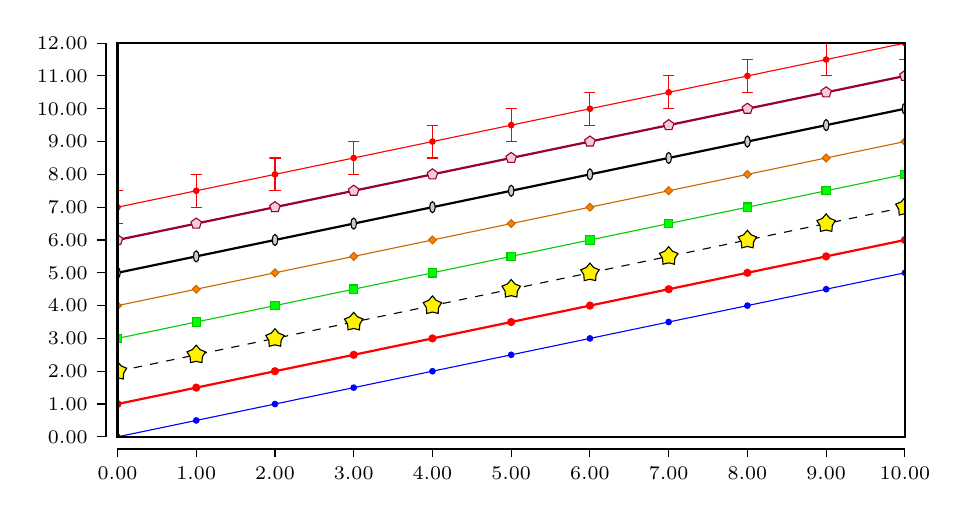
\begin{tikzpicture}[]
\begin{scope}[]
\clip (0,0) rectangle (10,5);
\begin{scope}[shift={(0.0,0.0)}]
\pgfsetxvec{\pgfpoint{1.0cm}{0cm}}
\pgfsetyvec{\pgfpoint{0cm}{0.41666666cm}}
\begin{scope}[blue]
\pgfpathmoveto{ \pgfqpointxy {0.0} {0.0}}
\pgfpathlineto{ \pgfqpointxy {1.0} {0.5}}
\pgfpathlineto{ \pgfqpointxy {2.0} {1.0}}
\pgfpathlineto{ \pgfqpointxy {3.0} {1.5}}
\pgfpathlineto{ \pgfqpointxy {4.0} {2.0}}
\pgfpathlineto{ \pgfqpointxy {5.0} {2.5}}
\pgfpathlineto{ \pgfqpointxy {6.0} {3.0}}
\pgfpathlineto{ \pgfqpointxy {7.0} {3.5}}
\pgfpathlineto{ \pgfqpointxy {8.0} {4.0}}
\pgfpathlineto{ \pgfqpointxy {9.0} {4.5}}
\pgfpathlineto{ \pgfqpointxy {10.0} {5.0}}
\pgfusepath{ stroke }
\end{scope}
\node at (0.0,0.0) [circle,inner sep=0pt,minimum width =2pt,minimum height=2pt,fill=blue,draw=blue] {}; 
\node at (1.0,0.5) [circle,inner sep=0pt,minimum width =2pt,minimum height=2pt,fill=blue,draw=blue] {}; 
\node at (2.0,1.0) [circle,inner sep=0pt,minimum width =2pt,minimum height=2pt,fill=blue,draw=blue] {}; 
\node at (3.0,1.5) [circle,inner sep=0pt,minimum width =2pt,minimum height=2pt,fill=blue,draw=blue] {}; 
\node at (4.0,2.0) [circle,inner sep=0pt,minimum width =2pt,minimum height=2pt,fill=blue,draw=blue] {}; 
\node at (5.0,2.5) [circle,inner sep=0pt,minimum width =2pt,minimum height=2pt,fill=blue,draw=blue] {}; 
\node at (6.0,3.0) [circle,inner sep=0pt,minimum width =2pt,minimum height=2pt,fill=blue,draw=blue] {}; 
\node at (7.0,3.5) [circle,inner sep=0pt,minimum width =2pt,minimum height=2pt,fill=blue,draw=blue] {}; 
\node at (8.0,4.0) [circle,inner sep=0pt,minimum width =2pt,minimum height=2pt,fill=blue,draw=blue] {}; 
\node at (9.0,4.5) [circle,inner sep=0pt,minimum width =2pt,minimum height=2pt,fill=blue,draw=blue] {}; 
\node at (10.0,5.0) [circle,inner sep=0pt,minimum width =2pt,minimum height=2pt,fill=blue,draw=blue] {}; 
\begin{scope}[red,thick]
\pgfpathmoveto{ \pgfqpointxy {0.0} {1.0}}
\pgfpathlineto{ \pgfqpointxy {1.0} {1.5}}
\pgfpathlineto{ \pgfqpointxy {2.0} {2.0}}
\pgfpathlineto{ \pgfqpointxy {3.0} {2.5}}
\pgfpathlineto{ \pgfqpointxy {4.0} {3.0}}
\pgfpathlineto{ \pgfqpointxy {5.0} {3.5}}
\pgfpathlineto{ \pgfqpointxy {6.0} {4.0}}
\pgfpathlineto{ \pgfqpointxy {7.0} {4.5}}
\pgfpathlineto{ \pgfqpointxy {8.0} {5.0}}
\pgfpathlineto{ \pgfqpointxy {9.0} {5.5}}
\pgfpathlineto{ \pgfqpointxy {10.0} {6.0}}
\pgfusepath{ stroke }
\end{scope}
\node at (0.0,1.0) [circle,inner sep=0pt,minimum width =3pt,minimum height=3pt,fill=red] {}; 
\node at (1.0,1.5) [circle,inner sep=0pt,minimum width =3pt,minimum height=3pt,fill=red] {}; 
\node at (2.0,2.0) [circle,inner sep=0pt,minimum width =3pt,minimum height=3pt,fill=red] {}; 
\node at (3.0,2.5) [circle,inner sep=0pt,minimum width =3pt,minimum height=3pt,fill=red] {}; 
\node at (4.0,3.0) [circle,inner sep=0pt,minimum width =3pt,minimum height=3pt,fill=red] {}; 
\node at (5.0,3.5) [circle,inner sep=0pt,minimum width =3pt,minimum height=3pt,fill=red] {}; 
\node at (6.0,4.0) [circle,inner sep=0pt,minimum width =3pt,minimum height=3pt,fill=red] {}; 
\node at (7.0,4.5) [circle,inner sep=0pt,minimum width =3pt,minimum height=3pt,fill=red] {}; 
\node at (8.0,5.0) [circle,inner sep=0pt,minimum width =3pt,minimum height=3pt,fill=red] {}; 
\node at (9.0,5.5) [circle,inner sep=0pt,minimum width =3pt,minimum height=3pt,fill=red] {}; 
\node at (10.0,6.0) [circle,inner sep=0pt,minimum width =3pt,minimum height=3pt,fill=red] {}; 
\begin{scope}[black,dashed]
\pgfpathmoveto{ \pgfqpointxy {0.0} {2.0}}
\pgfpathlineto{ \pgfqpointxy {1.0} {2.5}}
\pgfpathlineto{ \pgfqpointxy {2.0} {3.0}}
\pgfpathlineto{ \pgfqpointxy {3.0} {3.5}}
\pgfpathlineto{ \pgfqpointxy {4.0} {4.0}}
\pgfpathlineto{ \pgfqpointxy {5.0} {4.5}}
\pgfpathlineto{ \pgfqpointxy {6.0} {5.0}}
\pgfpathlineto{ \pgfqpointxy {7.0} {5.5}}
\pgfpathlineto{ \pgfqpointxy {8.0} {6.0}}
\pgfpathlineto{ \pgfqpointxy {9.0} {6.5}}
\pgfpathlineto{ \pgfqpointxy {10.0} {7.0}}
\pgfusepath{ stroke }
\end{scope}
\node at (0.0,2.0) [star,star points=5,inner sep=0pt,minimum width =7pt,minimum height=7pt,draw=black,fill=yellow] {}; 
\node at (1.0,2.5) [star,star points=5,inner sep=0pt,minimum width =7pt,minimum height=7pt,draw=black,fill=yellow] {}; 
\node at (2.0,3.0) [star,star points=5,inner sep=0pt,minimum width =7pt,minimum height=7pt,draw=black,fill=yellow] {}; 
\node at (3.0,3.5) [star,star points=5,inner sep=0pt,minimum width =7pt,minimum height=7pt,draw=black,fill=yellow] {}; 
\node at (4.0,4.0) [star,star points=5,inner sep=0pt,minimum width =7pt,minimum height=7pt,draw=black,fill=yellow] {}; 
\node at (5.0,4.5) [star,star points=5,inner sep=0pt,minimum width =7pt,minimum height=7pt,draw=black,fill=yellow] {}; 
\node at (6.0,5.0) [star,star points=5,inner sep=0pt,minimum width =7pt,minimum height=7pt,draw=black,fill=yellow] {}; 
\node at (7.0,5.5) [star,star points=5,inner sep=0pt,minimum width =7pt,minimum height=7pt,draw=black,fill=yellow] {}; 
\node at (8.0,6.0) [star,star points=5,inner sep=0pt,minimum width =7pt,minimum height=7pt,draw=black,fill=yellow] {}; 
\node at (9.0,6.5) [star,star points=5,inner sep=0pt,minimum width =7pt,minimum height=7pt,draw=black,fill=yellow] {}; 
\node at (10.0,7.0) [star,star points=5,inner sep=0pt,minimum width =7pt,minimum height=7pt,draw=black,fill=yellow] {}; 
\begin{scope}[green!80!black]
\pgfpathmoveto{ \pgfqpointxy {0.0} {3.0}}
\pgfpathlineto{ \pgfqpointxy {1.0} {3.5}}
\pgfpathlineto{ \pgfqpointxy {2.0} {4.0}}
\pgfpathlineto{ \pgfqpointxy {3.0} {4.5}}
\pgfpathlineto{ \pgfqpointxy {4.0} {5.0}}
\pgfpathlineto{ \pgfqpointxy {5.0} {5.5}}
\pgfpathlineto{ \pgfqpointxy {6.0} {6.0}}
\pgfpathlineto{ \pgfqpointxy {7.0} {6.5}}
\pgfpathlineto{ \pgfqpointxy {8.0} {7.0}}
\pgfpathlineto{ \pgfqpointxy {9.0} {7.5}}
\pgfpathlineto{ \pgfqpointxy {10.0} {8.0}}
\pgfusepath{ stroke }
\end{scope}
\node at (0.0,3.0) [rectangle,inner sep=0pt,minimum width =3pt,minimum height=3pt,draw=green!80!black,fill=green] {}; 
\node at (1.0,3.5) [rectangle,inner sep=0pt,minimum width =3pt,minimum height=3pt,draw=green!80!black,fill=green] {}; 
\node at (2.0,4.0) [rectangle,inner sep=0pt,minimum width =3pt,minimum height=3pt,draw=green!80!black,fill=green] {}; 
\node at (3.0,4.5) [rectangle,inner sep=0pt,minimum width =3pt,minimum height=3pt,draw=green!80!black,fill=green] {}; 
\node at (4.0,5.0) [rectangle,inner sep=0pt,minimum width =3pt,minimum height=3pt,draw=green!80!black,fill=green] {}; 
\node at (5.0,5.5) [rectangle,inner sep=0pt,minimum width =3pt,minimum height=3pt,draw=green!80!black,fill=green] {}; 
\node at (6.0,6.0) [rectangle,inner sep=0pt,minimum width =3pt,minimum height=3pt,draw=green!80!black,fill=green] {}; 
\node at (7.0,6.5) [rectangle,inner sep=0pt,minimum width =3pt,minimum height=3pt,draw=green!80!black,fill=green] {}; 
\node at (8.0,7.0) [rectangle,inner sep=0pt,minimum width =3pt,minimum height=3pt,draw=green!80!black,fill=green] {}; 
\node at (9.0,7.5) [rectangle,inner sep=0pt,minimum width =3pt,minimum height=3pt,draw=green!80!black,fill=green] {}; 
\node at (10.0,8.0) [rectangle,inner sep=0pt,minimum width =3pt,minimum height=3pt,draw=green!80!black,fill=green] {}; 
\begin{scope}[orange!80!black]
\pgfpathmoveto{ \pgfqpointxy {0.0} {4.0}}
\pgfpathlineto{ \pgfqpointxy {1.0} {4.5}}
\pgfpathlineto{ \pgfqpointxy {2.0} {5.0}}
\pgfpathlineto{ \pgfqpointxy {3.0} {5.5}}
\pgfpathlineto{ \pgfqpointxy {4.0} {6.0}}
\pgfpathlineto{ \pgfqpointxy {5.0} {6.5}}
\pgfpathlineto{ \pgfqpointxy {6.0} {7.0}}
\pgfpathlineto{ \pgfqpointxy {7.0} {7.5}}
\pgfpathlineto{ \pgfqpointxy {8.0} {8.0}}
\pgfpathlineto{ \pgfqpointxy {9.0} {8.5}}
\pgfpathlineto{ \pgfqpointxy {10.0} {9.0}}
\pgfusepath{ stroke }
\end{scope}
\node at (0.0,4.0) [diamond,inner sep=0pt,minimum width =3pt,minimum height=3pt,draw=orange!80!black,fill=orange] {}; 
\node at (1.0,4.5) [diamond,inner sep=0pt,minimum width =3pt,minimum height=3pt,draw=orange!80!black,fill=orange] {}; 
\node at (2.0,5.0) [diamond,inner sep=0pt,minimum width =3pt,minimum height=3pt,draw=orange!80!black,fill=orange] {}; 
\node at (3.0,5.5) [diamond,inner sep=0pt,minimum width =3pt,minimum height=3pt,draw=orange!80!black,fill=orange] {}; 
\node at (4.0,6.0) [diamond,inner sep=0pt,minimum width =3pt,minimum height=3pt,draw=orange!80!black,fill=orange] {}; 
\node at (5.0,6.5) [diamond,inner sep=0pt,minimum width =3pt,minimum height=3pt,draw=orange!80!black,fill=orange] {}; 
\node at (6.0,7.0) [diamond,inner sep=0pt,minimum width =3pt,minimum height=3pt,draw=orange!80!black,fill=orange] {}; 
\node at (7.0,7.5) [diamond,inner sep=0pt,minimum width =3pt,minimum height=3pt,draw=orange!80!black,fill=orange] {}; 
\node at (8.0,8.0) [diamond,inner sep=0pt,minimum width =3pt,minimum height=3pt,draw=orange!80!black,fill=orange] {}; 
\node at (9.0,8.5) [diamond,inner sep=0pt,minimum width =3pt,minimum height=3pt,draw=orange!80!black,fill=orange] {}; 
\node at (10.0,9.0) [diamond,inner sep=0pt,minimum width =3pt,minimum height=3pt,draw=orange!80!black,fill=orange] {}; 
\begin{scope}[black,thick]
\pgfpathmoveto{ \pgfqpointxy {0.0} {5.0}}
\pgfpathlineto{ \pgfqpointxy {1.0} {5.5}}
\pgfpathlineto{ \pgfqpointxy {2.0} {6.0}}
\pgfpathlineto{ \pgfqpointxy {3.0} {6.5}}
\pgfpathlineto{ \pgfqpointxy {4.0} {7.0}}
\pgfpathlineto{ \pgfqpointxy {5.0} {7.5}}
\pgfpathlineto{ \pgfqpointxy {6.0} {8.0}}
\pgfpathlineto{ \pgfqpointxy {7.0} {8.5}}
\pgfpathlineto{ \pgfqpointxy {8.0} {9.0}}
\pgfpathlineto{ \pgfqpointxy {9.0} {9.5}}
\pgfpathlineto{ \pgfqpointxy {10.0} {10.0}}
\pgfusepath{ stroke }
\end{scope}
\node at (0.0,5.0) [ellipse,inner sep=0pt,minimum width =2pt,minimum height=4pt,draw=black,fill=black!20] {}; 
\node at (1.0,5.5) [ellipse,inner sep=0pt,minimum width =2pt,minimum height=4pt,draw=black,fill=black!20] {}; 
\node at (2.0,6.0) [ellipse,inner sep=0pt,minimum width =2pt,minimum height=4pt,draw=black,fill=black!20] {}; 
\node at (3.0,6.5) [ellipse,inner sep=0pt,minimum width =2pt,minimum height=4pt,draw=black,fill=black!20] {}; 
\node at (4.0,7.0) [ellipse,inner sep=0pt,minimum width =2pt,minimum height=4pt,draw=black,fill=black!20] {}; 
\node at (5.0,7.5) [ellipse,inner sep=0pt,minimum width =2pt,minimum height=4pt,draw=black,fill=black!20] {}; 
\node at (6.0,8.0) [ellipse,inner sep=0pt,minimum width =2pt,minimum height=4pt,draw=black,fill=black!20] {}; 
\node at (7.0,8.5) [ellipse,inner sep=0pt,minimum width =2pt,minimum height=4pt,draw=black,fill=black!20] {}; 
\node at (8.0,9.0) [ellipse,inner sep=0pt,minimum width =2pt,minimum height=4pt,draw=black,fill=black!20] {}; 
\node at (9.0,9.5) [ellipse,inner sep=0pt,minimum width =2pt,minimum height=4pt,draw=black,fill=black!20] {}; 
\node at (10.0,10.0) [ellipse,inner sep=0pt,minimum width =2pt,minimum height=4pt,draw=black,fill=black!20] {}; 
\begin{scope}[purple!80!black,thick]
\pgfpathmoveto{ \pgfqpointxy {0.0} {6.0}}
\pgfpathlineto{ \pgfqpointxy {1.0} {6.5}}
\pgfpathlineto{ \pgfqpointxy {2.0} {7.0}}
\pgfpathlineto{ \pgfqpointxy {3.0} {7.5}}
\pgfpathlineto{ \pgfqpointxy {4.0} {8.0}}
\pgfpathlineto{ \pgfqpointxy {5.0} {8.5}}
\pgfpathlineto{ \pgfqpointxy {6.0} {9.0}}
\pgfpathlineto{ \pgfqpointxy {7.0} {9.5}}
\pgfpathlineto{ \pgfqpointxy {8.0} {10.0}}
\pgfpathlineto{ \pgfqpointxy {9.0} {10.5}}
\pgfpathlineto{ \pgfqpointxy {10.0} {11.0}}
\pgfusepath{ stroke }
\end{scope}
\node at (0.0,6.0) [regular polygon,regular polygon sides=5,inner sep=0pt,minimum width =4pt,minimum height=4pt,draw=purple!80!black,fill=purple!20] {}; 
\node at (1.0,6.5) [regular polygon,regular polygon sides=5,inner sep=0pt,minimum width =4pt,minimum height=4pt,draw=purple!80!black,fill=purple!20] {}; 
\node at (2.0,7.0) [regular polygon,regular polygon sides=5,inner sep=0pt,minimum width =4pt,minimum height=4pt,draw=purple!80!black,fill=purple!20] {}; 
\node at (3.0,7.5) [regular polygon,regular polygon sides=5,inner sep=0pt,minimum width =4pt,minimum height=4pt,draw=purple!80!black,fill=purple!20] {}; 
\node at (4.0,8.0) [regular polygon,regular polygon sides=5,inner sep=0pt,minimum width =4pt,minimum height=4pt,draw=purple!80!black,fill=purple!20] {}; 
\node at (5.0,8.5) [regular polygon,regular polygon sides=5,inner sep=0pt,minimum width =4pt,minimum height=4pt,draw=purple!80!black,fill=purple!20] {}; 
\node at (6.0,9.0) [regular polygon,regular polygon sides=5,inner sep=0pt,minimum width =4pt,minimum height=4pt,draw=purple!80!black,fill=purple!20] {}; 
\node at (7.0,9.5) [regular polygon,regular polygon sides=5,inner sep=0pt,minimum width =4pt,minimum height=4pt,draw=purple!80!black,fill=purple!20] {}; 
\node at (8.0,10.0) [regular polygon,regular polygon sides=5,inner sep=0pt,minimum width =4pt,minimum height=4pt,draw=purple!80!black,fill=purple!20] {}; 
\node at (9.0,10.5) [regular polygon,regular polygon sides=5,inner sep=0pt,minimum width =4pt,minimum height=4pt,draw=purple!80!black,fill=purple!20] {}; 
\node at (10.0,11.0) [regular polygon,regular polygon sides=5,inner sep=0pt,minimum width =4pt,minimum height=4pt,draw=purple!80!black,fill=purple!20] {}; 
\begin{scope}[red]
\pgfpathmoveto{ \pgfqpointxy {0.0} {7.0}}
\pgfpathlineto{ \pgfqpointxy {1.0} {7.5}}
\pgfpathlineto{ \pgfqpointxy {2.0} {8.0}}
\pgfpathlineto{ \pgfqpointxy {3.0} {8.5}}
\pgfpathlineto{ \pgfqpointxy {4.0} {9.0}}
\pgfpathlineto{ \pgfqpointxy {5.0} {9.5}}
\pgfpathlineto{ \pgfqpointxy {6.0} {10.0}}
\pgfpathlineto{ \pgfqpointxy {7.0} {10.5}}
\pgfpathlineto{ \pgfqpointxy {8.0} {11.0}}
\pgfpathlineto{ \pgfqpointxy {9.0} {11.5}}
\pgfpathlineto{ \pgfqpointxy {10.0} {12.0}}
\pgfusepath{ stroke }
\end{scope}
\begin{scope}[draw=red,fill=red]
\pgfpathmoveto{ \pgfqpointxy {0.0} {6.5}}
\pgfpathlineto{ \pgfqpointxy {0.0} {7.5}}
\pgfusepath{ stroke }
\end{scope}
\node at (0.0,7.0) [circle,inner sep=0pt,minimum width =2pt,minimum height=2pt,draw=red,fill=red] {}; 
\begin{scope}[draw=red,fill=red]
\pgfpathmoveto{ \pgfpointadd{\pgfqpointxy {0.0} {7.5}} {\pgfpoint{2pt}{0}}}
\pgfpathlineto{ \pgfpointadd{\pgfqpointxy {0.0} {7.5}} {\pgfpoint{-2pt}{0}}}
\pgfpathlineto{ \pgfqpointxy {0.0} {7.5}}
\pgfpathlineto{ \pgfqpointxy {0.0} {6.5}}
\pgfpathmoveto{ \pgfpointadd{\pgfqpointxy {0.0} {6.5}} {\pgfpoint {2pt} {0} }}
\pgfpathlineto{ \pgfpointadd{\pgfqpointxy {0.0} {6.5}} {\pgfpoint {-2pt} {0} }}
\pgfusepath{ stroke }
\end{scope}
\begin{scope}[draw=red,fill=red]
\pgfpathmoveto{ \pgfqpointxy {1.0} {7.0}}
\pgfpathlineto{ \pgfqpointxy {1.0} {8.0}}
\pgfusepath{ stroke }
\end{scope}
\node at (1.0,7.5) [circle,inner sep=0pt,minimum width =2pt,minimum height=2pt,draw=red,fill=red] {}; 
\begin{scope}[draw=red,fill=red]
\pgfpathmoveto{ \pgfpointadd{\pgfqpointxy {1.0} {8.0}} {\pgfpoint{2pt}{0}}}
\pgfpathlineto{ \pgfpointadd{\pgfqpointxy {1.0} {8.0}} {\pgfpoint{-2pt}{0}}}
\pgfpathlineto{ \pgfqpointxy {1.0} {8.0}}
\pgfpathlineto{ \pgfqpointxy {1.0} {7.0}}
\pgfpathmoveto{ \pgfpointadd{\pgfqpointxy {1.0} {7.0}} {\pgfpoint {2pt} {0} }}
\pgfpathlineto{ \pgfpointadd{\pgfqpointxy {1.0} {7.0}} {\pgfpoint {-2pt} {0} }}
\pgfusepath{ stroke }
\end{scope}
\begin{scope}[draw=red,fill=red]
\pgfpathmoveto{ \pgfqpointxy {2.0} {7.5}}
\pgfpathlineto{ \pgfqpointxy {2.0} {8.5}}
\pgfusepath{ stroke }
\end{scope}
\node at (2.0,8.0) [circle,inner sep=0pt,minimum width =2pt,minimum height=2pt,draw=red,fill=red] {}; 
\begin{scope}[draw=red,fill=red]
\pgfpathmoveto{ \pgfpointadd{\pgfqpointxy {2.0} {8.5}} {\pgfpoint{2pt}{0}}}
\pgfpathlineto{ \pgfpointadd{\pgfqpointxy {2.0} {8.5}} {\pgfpoint{-2pt}{0}}}
\pgfpathlineto{ \pgfqpointxy {2.0} {8.5}}
\pgfpathlineto{ \pgfqpointxy {2.0} {7.5}}
\pgfpathmoveto{ \pgfpointadd{\pgfqpointxy {2.0} {7.5}} {\pgfpoint {2pt} {0} }}
\pgfpathlineto{ \pgfpointadd{\pgfqpointxy {2.0} {7.5}} {\pgfpoint {-2pt} {0} }}
\pgfusepath{ stroke }
\end{scope}
\begin{scope}[draw=red,fill=red]
\pgfpathmoveto{ \pgfqpointxy {3.0} {8.0}}
\pgfpathlineto{ \pgfqpointxy {3.0} {9.0}}
\pgfusepath{ stroke }
\end{scope}
\node at (3.0,8.5) [circle,inner sep=0pt,minimum width =2pt,minimum height=2pt,draw=red,fill=red] {}; 
\begin{scope}[draw=red,fill=red]
\pgfpathmoveto{ \pgfpointadd{\pgfqpointxy {3.0} {9.0}} {\pgfpoint{2pt}{0}}}
\pgfpathlineto{ \pgfpointadd{\pgfqpointxy {3.0} {9.0}} {\pgfpoint{-2pt}{0}}}
\pgfpathlineto{ \pgfqpointxy {3.0} {9.0}}
\pgfpathlineto{ \pgfqpointxy {3.0} {8.0}}
\pgfpathmoveto{ \pgfpointadd{\pgfqpointxy {3.0} {8.0}} {\pgfpoint {2pt} {0} }}
\pgfpathlineto{ \pgfpointadd{\pgfqpointxy {3.0} {8.0}} {\pgfpoint {-2pt} {0} }}
\pgfusepath{ stroke }
\end{scope}
\begin{scope}[draw=red,fill=red]
\pgfpathmoveto{ \pgfqpointxy {4.0} {8.5}}
\pgfpathlineto{ \pgfqpointxy {4.0} {9.5}}
\pgfusepath{ stroke }
\end{scope}
\node at (4.0,9.0) [circle,inner sep=0pt,minimum width =2pt,minimum height=2pt,draw=red,fill=red] {}; 
\begin{scope}[draw=red,fill=red]
\pgfpathmoveto{ \pgfpointadd{\pgfqpointxy {4.0} {9.5}} {\pgfpoint{2pt}{0}}}
\pgfpathlineto{ \pgfpointadd{\pgfqpointxy {4.0} {9.5}} {\pgfpoint{-2pt}{0}}}
\pgfpathlineto{ \pgfqpointxy {4.0} {9.5}}
\pgfpathlineto{ \pgfqpointxy {4.0} {8.5}}
\pgfpathmoveto{ \pgfpointadd{\pgfqpointxy {4.0} {8.5}} {\pgfpoint {2pt} {0} }}
\pgfpathlineto{ \pgfpointadd{\pgfqpointxy {4.0} {8.5}} {\pgfpoint {-2pt} {0} }}
\pgfusepath{ stroke }
\end{scope}
\begin{scope}[draw=red,fill=red]
\pgfpathmoveto{ \pgfqpointxy {5.0} {9.0}}
\pgfpathlineto{ \pgfqpointxy {5.0} {10.0}}
\pgfusepath{ stroke }
\end{scope}
\node at (5.0,9.5) [circle,inner sep=0pt,minimum width =2pt,minimum height=2pt,draw=red,fill=red] {}; 
\begin{scope}[draw=red,fill=red]
\pgfpathmoveto{ \pgfpointadd{\pgfqpointxy {5.0} {10.0}} {\pgfpoint{2pt}{0}}}
\pgfpathlineto{ \pgfpointadd{\pgfqpointxy {5.0} {10.0}} {\pgfpoint{-2pt}{0}}}
\pgfpathlineto{ \pgfqpointxy {5.0} {10.0}}
\pgfpathlineto{ \pgfqpointxy {5.0} {9.0}}
\pgfpathmoveto{ \pgfpointadd{\pgfqpointxy {5.0} {9.0}} {\pgfpoint {2pt} {0} }}
\pgfpathlineto{ \pgfpointadd{\pgfqpointxy {5.0} {9.0}} {\pgfpoint {-2pt} {0} }}
\pgfusepath{ stroke }
\end{scope}
\begin{scope}[draw=red,fill=red]
\pgfpathmoveto{ \pgfqpointxy {6.0} {9.5}}
\pgfpathlineto{ \pgfqpointxy {6.0} {10.5}}
\pgfusepath{ stroke }
\end{scope}
\node at (6.0,10.0) [circle,inner sep=0pt,minimum width =2pt,minimum height=2pt,draw=red,fill=red] {}; 
\begin{scope}[draw=red,fill=red]
\pgfpathmoveto{ \pgfpointadd{\pgfqpointxy {6.0} {10.5}} {\pgfpoint{2pt}{0}}}
\pgfpathlineto{ \pgfpointadd{\pgfqpointxy {6.0} {10.5}} {\pgfpoint{-2pt}{0}}}
\pgfpathlineto{ \pgfqpointxy {6.0} {10.5}}
\pgfpathlineto{ \pgfqpointxy {6.0} {9.5}}
\pgfpathmoveto{ \pgfpointadd{\pgfqpointxy {6.0} {9.5}} {\pgfpoint {2pt} {0} }}
\pgfpathlineto{ \pgfpointadd{\pgfqpointxy {6.0} {9.5}} {\pgfpoint {-2pt} {0} }}
\pgfusepath{ stroke }
\end{scope}
\begin{scope}[draw=red,fill=red]
\pgfpathmoveto{ \pgfqpointxy {7.0} {10.0}}
\pgfpathlineto{ \pgfqpointxy {7.0} {11.0}}
\pgfusepath{ stroke }
\end{scope}
\node at (7.0,10.5) [circle,inner sep=0pt,minimum width =2pt,minimum height=2pt,draw=red,fill=red] {}; 
\begin{scope}[draw=red,fill=red]
\pgfpathmoveto{ \pgfpointadd{\pgfqpointxy {7.0} {11.0}} {\pgfpoint{2pt}{0}}}
\pgfpathlineto{ \pgfpointadd{\pgfqpointxy {7.0} {11.0}} {\pgfpoint{-2pt}{0}}}
\pgfpathlineto{ \pgfqpointxy {7.0} {11.0}}
\pgfpathlineto{ \pgfqpointxy {7.0} {10.0}}
\pgfpathmoveto{ \pgfpointadd{\pgfqpointxy {7.0} {10.0}} {\pgfpoint {2pt} {0} }}
\pgfpathlineto{ \pgfpointadd{\pgfqpointxy {7.0} {10.0}} {\pgfpoint {-2pt} {0} }}
\pgfusepath{ stroke }
\end{scope}
\begin{scope}[draw=red,fill=red]
\pgfpathmoveto{ \pgfqpointxy {8.0} {10.5}}
\pgfpathlineto{ \pgfqpointxy {8.0} {11.5}}
\pgfusepath{ stroke }
\end{scope}
\node at (8.0,11.0) [circle,inner sep=0pt,minimum width =2pt,minimum height=2pt,draw=red,fill=red] {}; 
\begin{scope}[draw=red,fill=red]
\pgfpathmoveto{ \pgfpointadd{\pgfqpointxy {8.0} {11.5}} {\pgfpoint{2pt}{0}}}
\pgfpathlineto{ \pgfpointadd{\pgfqpointxy {8.0} {11.5}} {\pgfpoint{-2pt}{0}}}
\pgfpathlineto{ \pgfqpointxy {8.0} {11.5}}
\pgfpathlineto{ \pgfqpointxy {8.0} {10.5}}
\pgfpathmoveto{ \pgfpointadd{\pgfqpointxy {8.0} {10.5}} {\pgfpoint {2pt} {0} }}
\pgfpathlineto{ \pgfpointadd{\pgfqpointxy {8.0} {10.5}} {\pgfpoint {-2pt} {0} }}
\pgfusepath{ stroke }
\end{scope}
\begin{scope}[draw=red,fill=red]
\pgfpathmoveto{ \pgfqpointxy {9.0} {11.0}}
\pgfpathlineto{ \pgfqpointxy {9.0} {12.0}}
\pgfusepath{ stroke }
\end{scope}
\node at (9.0,11.5) [circle,inner sep=0pt,minimum width =2pt,minimum height=2pt,draw=red,fill=red] {}; 
\begin{scope}[draw=red,fill=red]
\pgfpathmoveto{ \pgfpointadd{\pgfqpointxy {9.0} {12.0}} {\pgfpoint{2pt}{0}}}
\pgfpathlineto{ \pgfpointadd{\pgfqpointxy {9.0} {12.0}} {\pgfpoint{-2pt}{0}}}
\pgfpathlineto{ \pgfqpointxy {9.0} {12.0}}
\pgfpathlineto{ \pgfqpointxy {9.0} {11.0}}
\pgfpathmoveto{ \pgfpointadd{\pgfqpointxy {9.0} {11.0}} {\pgfpoint {2pt} {0} }}
\pgfpathlineto{ \pgfpointadd{\pgfqpointxy {9.0} {11.0}} {\pgfpoint {-2pt} {0} }}
\pgfusepath{ stroke }
\end{scope}
\begin{scope}[draw=red,fill=red]
\pgfpathmoveto{ \pgfqpointxy {10.0} {11.5}}
\pgfpathlineto{ \pgfqpointxy {10.0} {12.5}}
\pgfusepath{ stroke }
\end{scope}
\node at (10.0,12.0) [circle,inner sep=0pt,minimum width =2pt,minimum height=2pt,draw=red,fill=red] {}; 
\begin{scope}[draw=red,fill=red]
\pgfpathmoveto{ \pgfpointadd{\pgfqpointxy {10.0} {12.5}} {\pgfpoint{2pt}{0}}}
\pgfpathlineto{ \pgfpointadd{\pgfqpointxy {10.0} {12.5}} {\pgfpoint{-2pt}{0}}}
\pgfpathlineto{ \pgfqpointxy {10.0} {12.5}}
\pgfpathlineto{ \pgfqpointxy {10.0} {11.5}}
\pgfpathmoveto{ \pgfpointadd{\pgfqpointxy {10.0} {11.5}} {\pgfpoint {2pt} {0} }}
\pgfpathlineto{ \pgfpointadd{\pgfqpointxy {10.0} {11.5}} {\pgfpoint {-2pt} {0} }}
\pgfusepath{ stroke }
\end{scope}
\pgfsetxvec{\pgfpoint{1cm}{0cm}}
\pgfsetyvec{\pgfpoint{0cm}{1cm}}
\end{scope}
\end{scope}
\begin{scope}[shift={(0.0,0.0)}]
\pgfsetxvec{\pgfpoint{1.0cm}{0cm}}
\pgfsetyvec{\pgfpoint{0cm}{0.41666666cm}}
\begin{scope}[yshift=-0.15cm]
\draw[] [shift={(0.0,0.0)}] (0pt,0pt) -- (-0pt,-3pt) node[below]{ \scriptsize{\num[round-mode=places,round-precision=2]{0}}};
\draw[] [shift={(1.0,0.0)}] (0pt,0pt) -- (-0pt,-3pt) node[below]{ \scriptsize{\num[round-mode=places,round-precision=2]{1}}};
\draw[] [shift={(2.0,0.0)}] (0pt,0pt) -- (-0pt,-3pt) node[below]{ \scriptsize{\num[round-mode=places,round-precision=2]{2}}};
\draw[] [shift={(3.0,0.0)}] (0pt,0pt) -- (-0pt,-3pt) node[below]{ \scriptsize{\num[round-mode=places,round-precision=2]{3}}};
\draw[] [shift={(4.0,0.0)}] (0pt,0pt) -- (-0pt,-3pt) node[below]{ \scriptsize{\num[round-mode=places,round-precision=2]{4}}};
\draw[] [shift={(5.0,0.0)}] (0pt,0pt) -- (-0pt,-3pt) node[below]{ \scriptsize{\num[round-mode=places,round-precision=2]{5}}};
\draw[] [shift={(6.0,0.0)}] (0pt,0pt) -- (-0pt,-3pt) node[below]{ \scriptsize{\num[round-mode=places,round-precision=2]{6}}};
\draw[] [shift={(7.0,0.0)}] (0pt,0pt) -- (-0pt,-3pt) node[below]{ \scriptsize{\num[round-mode=places,round-precision=2]{7}}};
\draw[] [shift={(8.0,0.0)}] (0pt,0pt) -- (-0pt,-3pt) node[below]{ \scriptsize{\num[round-mode=places,round-precision=2]{8}}};
\draw[] [shift={(9.0,0.0)}] (0pt,0pt) -- (-0pt,-3pt) node[below]{ \scriptsize{\num[round-mode=places,round-precision=2]{9}}};
\draw[] [shift={(10.0,0.0)}] (0pt,0pt) -- (-0pt,-3pt) node[below]{ \scriptsize{\num[round-mode=places,round-precision=2]{10}}};
\end{scope}
\begin{scope}[xshift=-0.15cm]
\draw[] [shift={(0.0,0.0)}] (0pt,0pt) -- (-3pt,-0pt) node[left]{ \scriptsize{\num[round-mode=places,round-precision=2]{0}}};
\draw[] [shift={(0.0,1.0)}] (0pt,0pt) -- (-3pt,-0pt) node[left]{ \scriptsize{\num[round-mode=places,round-precision=2]{1}}};
\draw[] [shift={(0.0,2.0)}] (0pt,0pt) -- (-3pt,-0pt) node[left]{ \scriptsize{\num[round-mode=places,round-precision=2]{2}}};
\draw[] [shift={(0.0,3.0)}] (0pt,0pt) -- (-3pt,-0pt) node[left]{ \scriptsize{\num[round-mode=places,round-precision=2]{3}}};
\draw[] [shift={(0.0,4.0)}] (0pt,0pt) -- (-3pt,-0pt) node[left]{ \scriptsize{\num[round-mode=places,round-precision=2]{4}}};
\draw[] [shift={(0.0,5.0)}] (0pt,0pt) -- (-3pt,-0pt) node[left]{ \scriptsize{\num[round-mode=places,round-precision=2]{5}}};
\draw[] [shift={(0.0,6.0)}] (0pt,0pt) -- (-3pt,-0pt) node[left]{ \scriptsize{\num[round-mode=places,round-precision=2]{6}}};
\draw[] [shift={(0.0,7.0)}] (0pt,0pt) -- (-3pt,-0pt) node[left]{ \scriptsize{\num[round-mode=places,round-precision=2]{7}}};
\draw[] [shift={(0.0,8.0)}] (0pt,0pt) -- (-3pt,-0pt) node[left]{ \scriptsize{\num[round-mode=places,round-precision=2]{8}}};
\draw[] [shift={(0.0,9.0)}] (0pt,0pt) -- (-3pt,-0pt) node[left]{ \scriptsize{\num[round-mode=places,round-precision=2]{9}}};
\draw[] [shift={(0.0,10.0)}] (0pt,0pt) -- (-3pt,-0pt) node[left]{ \scriptsize{\num[round-mode=places,round-precision=2]{10}}};
\draw[] [shift={(0.0,11.0)}] (0pt,0pt) -- (-3pt,-0pt) node[left]{ \scriptsize{\num[round-mode=places,round-precision=2]{11}}};
\draw[] [shift={(0.0,12.0)}] (0pt,0pt) -- (-3pt,-0pt) node[left]{ \scriptsize{\num[round-mode=places,round-precision=2]{12}}};
\end{scope}
\pgfsetxvec{\pgfpoint{1cm}{0cm}}
\pgfsetyvec{\pgfpoint{0cm}{1cm}}
\end{scope}
\draw[black,thick] (0.0,-0.15) -- (10.0,-0.15);
\draw[black,thick] (-0.15,0.0) -- (-0.15,5.0);
\draw[thick] (0,0) rectangle (10,5);
\end{tikzpicture}
%%% Local Variables: 
%%% mode: latex 
%%% TeX-master: "master" 
%%% End:


\captionsetup{singlelinecheck=off}
\caption[asdf]{Different styles of lines and nodes. The styles are just regular tikz options.}
\end{figure}
\begin{figure}[H]
\centering
\documentclass{standalone}
\ifx\HCode\UnDef\else\def\pgfsysdriver{pgfsys-tex4ht.def}\fi
\usepackage[usenames,dvipsnames,svgnames,table]{xcolor}
\usepackage{tikz}
\usepackage{color}
\usepackage{siunitx}
\usetikzlibrary{arrows,shapes}
\begin{document}
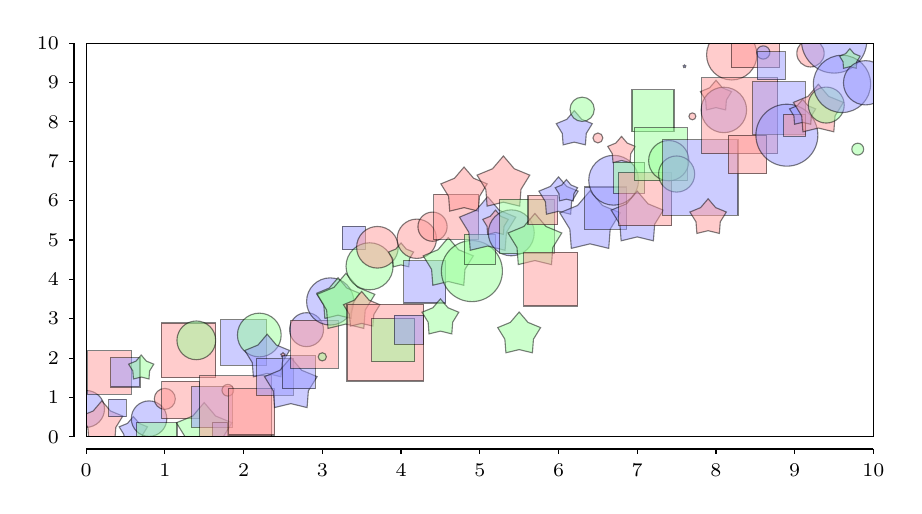
\begin{tikzpicture}
\begin{scope}[]
\pgfpathmoveto{ \pgfpointxy {0.0} {0.0}}
\pgfpathlineto{ \pgfpointxy {10.0} {0.0}}
\pgfpathlineto{ \pgfpointxy {10.0} {5.0}}
\pgfpathlineto{ \pgfpointxy {0.0} {5.0}}
\pgfpathclose
\pgfusepath{  clip, }
\begin{scope}[shift={(0.0,0.0)}]
\pgfsetxvec{\pgfpoint{1.0cm}{0cm}}
\pgfsetyvec{\pgfpoint{0cm}{0.5cm}}
\begin{scope}[shift={(0.0,0.0)}]
\node at (0.0,0.709579903064161) [draw=black,fill=blue!40,opacity=0.5,circle,inner sep=0.0mm,minimum width =4.684404387965109mm,minimum height=4.684404387965109mm] {};
\node at (0.1,-1.3086410799311836) [draw=black,fill=blue!40,opacity=0.5,circle,inner sep=0.0mm,minimum width =5.948432363904152mm,minimum height=5.948432363904152mm] {};
\node at (0.2,0.35464207368852163) [draw=black,fill=red!40,opacity=0.5,star,inner sep=0.0mm,minimum width =5.597520769773753mm,minimum height=5.597520769773753mm] {};
\node at (0.3,1.6355035193942828) [draw=black,fill=red!40,opacity=0.5,rectangle,inner sep=0.0mm,minimum width =5.5289513760349704mm,minimum height=5.5289513760349704mm] {};
\node at (0.4,0.7275541529298895) [draw=black,fill=blue!40,opacity=0.5,rectangle,inner sep=0.0mm,minimum width =2.2165720989965196mm,minimum height=2.2165720989965196mm] {};
\node at (0.5,1.6345911300381193) [draw=black,fill=blue!40,opacity=0.5,rectangle,inner sep=0.0mm,minimum width =3.69348293691323mm,minimum height=3.69348293691323mm] {};
\node at (0.6,0.1372935667470575) [draw=black,fill=blue!40,opacity=0.5,star,inner sep=0.0mm,minimum width =3.783654313145048mm,minimum height=3.783654313145048mm] {};
\node at (0.7,1.7421867243340636) [draw=black,fill=green!40,opacity=0.5,star,inner sep=0.0mm,minimum width =3.3580720084876603mm,minimum height=3.3580720084876603mm] {};
\node at (0.8,0.4620408089043557) [draw=black,fill=blue!40,opacity=0.5,circle,inner sep=0.0mm,minimum width =4.510210384891336mm,minimum height=4.510210384891336mm] {};
\node at (0.90000004,-0.15530240728422862) [draw=black,fill=green!40,opacity=0.5,rectangle,inner sep=0.0mm,minimum width =5.100643838385599mm,minimum height=5.100643838385599mm] {};
\node at (1.0,0.9641748075000852) [draw=black,fill=red!40,opacity=0.5,circle,inner sep=0.0mm,minimum width =2.673701415640892mm,minimum height=2.673701415640892mm] {};
\node at (1.1,-1.1603107800518702) [draw=black,fill=green!40,opacity=0.5,circle,inner sep=0.0mm,minimum width =4.774274002638963mm,minimum height=4.774274002638963mm] {};
\node at (1.2,0.9334271294075822) [draw=black,fill=red!40,opacity=0.5,rectangle,inner sep=0.0mm,minimum width =4.740705628150259mm,minimum height=4.740705628150259mm] {};
\node at (1.3000001,2.196453840862024) [draw=black,fill=red!40,opacity=0.5,rectangle,inner sep=0.0mm,minimum width =6.953264139897893mm,minimum height=6.953264139897893mm] {};
\node at (1.4,2.4509401059034674) [draw=black,fill=green!40,opacity=0.5,circle,inner sep=0.0mm,minimum width =4.918409651642974mm,minimum height=4.918409651642974mm] {};
\node at (1.5,0.1287607390986354) [draw=black,fill=green!40,opacity=0.5,star,inner sep=0.0mm,minimum width =7.414065824401571mm,minimum height=7.414065824401571mm] {};
\node at (1.6,0.7619799504504053) [draw=black,fill=blue!40,opacity=0.5,rectangle,inner sep=0.0mm,minimum width =5.155594127275793mm,minimum height=5.155594127275793mm] {};
\node at (1.7,0.18446059842809426) [draw=black,fill=blue!40,opacity=0.5,rectangle,inner sep=0.0mm,minimum width =1.8236676531537817mm,minimum height=1.8236676531537817mm] {};
\node at (1.8000001,1.1832418888351939) [draw=black,fill=red!40,opacity=0.5,circle,inner sep=0.0mm,minimum width =1.483075043186194mm,minimum height=1.483075043186194mm] {};
\node at (1.9,0.6438811288709911) [draw=black,fill=red!40,opacity=0.5,rectangle,inner sep=0.0mm,minimum width =9.121229801796648mm,minimum height=9.121229801796648mm] {};
\node at (2.0,2.399988531779001) [draw=black,fill=blue!40,opacity=0.5,rectangle,inner sep=0.0mm,minimum width =5.790814399699697mm,minimum height=5.790814399699697mm] {};
\node at (2.1000001,0.6336931157661692) [draw=black,fill=red!40,opacity=0.5,rectangle,inner sep=0.0mm,minimum width =5.883046419335988mm,minimum height=5.883046419335988mm] {};
\node at (2.2,2.5863110861604133) [draw=black,fill=green!40,opacity=0.5,circle,inner sep=0.0mm,minimum width =5.5551403318859105mm,minimum height=5.5551403318859105mm] {};
\node at (2.3,2.0088235911851084) [draw=black,fill=blue!40,opacity=0.5,star,inner sep=0.0mm,minimum width =5.978204784282441mm,minimum height=5.978204784282441mm] {};
\node at (2.4,1.5184735280897157) [draw=black,fill=blue!40,opacity=0.5,rectangle,inner sep=0.0mm,minimum width =4.6291829657364465mm,minimum height=4.6291829657364465mm] {};
\node at (2.5,2.081125610249627) [draw=black,fill=red!40,opacity=0.5,star,inner sep=0.0mm,minimum width =0.5808451501325136mm,minimum height=0.5808451501325136mm] {};
\node at (2.6000001,1.312119941776202) [draw=black,fill=blue!40,opacity=0.5,star,inner sep=0.0mm,minimum width =7.028290655475499mm,minimum height=7.028290655475499mm] {};
\node at (2.7,1.637236852472321) [draw=black,fill=blue!40,opacity=0.5,rectangle,inner sep=0.0mm,minimum width =4.1993268052830075mm,minimum height=4.1993268052830075mm] {};
\node at (2.8,2.722482173813692) [draw=black,fill=blue!40,opacity=0.5,circle,inner sep=0.0mm,minimum width =4.310358115557271mm,minimum height=4.310358115557271mm] {};
\node at (2.9,2.3523726337683586) [draw=black,fill=red!40,opacity=0.5,rectangle,inner sep=0.0mm,minimum width =6.057682425604773mm,minimum height=6.057682425604773mm] {};
\node at (3.0,2.0324011303461686) [draw=black,fill=green!40,opacity=0.5,circle,inner sep=0.0mm,minimum width =1.040741659203983mm,minimum height=1.040741659203983mm] {};
\node at (3.1000001,3.438578408970455) [draw=black,fill=blue!40,opacity=0.5,circle,inner sep=0.0mm,minimum width =5.995604978545116mm,minimum height=5.995604978545116mm] {};
\node at (3.2,3.4707427399239204) [draw=black,fill=green!40,opacity=0.5,star,inner sep=0.0mm,minimum width =5.710271475224298mm,minimum height=5.710271475224298mm] {};
\node at (3.3,3.379956079683047) [draw=black,fill=green!40,opacity=0.5,star,inner sep=0.0mm,minimum width =7.728879228930112mm,minimum height=7.728879228930112mm] {};
\node at (3.4,5.050936643838629) [draw=black,fill=blue!40,opacity=0.5,rectangle,inner sep=0.0mm,minimum width =2.9447285286666793mm,minimum height=2.9447285286666793mm] {};
\node at (3.5,3.2059979135589516) [draw=black,fill=red!40,opacity=0.5,star,inner sep=0.0mm,minimum width =4.868690569045189mm,minimum height=4.868690569045189mm] {};
\node at (3.6000001,4.3317506628087346) [draw=black,fill=green!40,opacity=0.5,circle,inner sep=0.0mm,minimum width =5.9754418095417074mm,minimum height=5.9754418095417074mm] {};
\node at (3.7,4.814904111132433) [draw=black,fill=red!40,opacity=0.5,circle,inner sep=0.0mm,minimum width =5.288882938019944mm,minimum height=5.288882938019944mm] {};
\node at (3.8,2.391690563293844) [draw=black,fill=red!40,opacity=0.5,rectangle,inner sep=0.0mm,minimum width =9.728440412869261mm,minimum height=9.728440412869261mm] {};
\node at (3.9,2.4498473067093514) [draw=black,fill=green!40,opacity=0.5,rectangle,inner sep=0.0mm,minimum width =5.4504184785211285mm,minimum height=5.4504184785211285mm] {};
\node at (4.0,4.589797853575581) [draw=black,fill=green!40,opacity=0.5,star,inner sep=0.0mm,minimum width =3.345428851666787mm,minimum height=3.345428851666787mm] {};
\node at (4.1,2.724158727310493) [draw=black,fill=blue!40,opacity=0.5,rectangle,inner sep=0.0mm,minimum width =3.6857011733674985mm,minimum height=3.6857011733674985mm] {};
\node at (4.2000003,5.0312764967330335) [draw=black,fill=red!40,opacity=0.5,circle,inner sep=0.0mm,minimum width =4.99519411089988mm,minimum height=4.99519411089988mm] {};
\node at (4.3,3.9348257471569066) [draw=black,fill=blue!40,opacity=0.5,rectangle,inner sep=0.0mm,minimum width =5.342270493568651mm,minimum height=5.342270493568651mm] {};
\node at (4.4,5.338033392113277) [draw=black,fill=red!40,opacity=0.5,circle,inner sep=0.0mm,minimum width =3.7076063582040835mm,minimum height=3.7076063582040835mm] {};
\node at (4.5,3.0129312560328323) [draw=black,fill=green!40,opacity=0.5,star,inner sep=0.0mm,minimum width =4.915535481344827mm,minimum height=4.915535481344827mm] {};
\node at (4.6,4.391119711430295) [draw=black,fill=green!40,opacity=0.5,star,inner sep=0.0mm,minimum width =6.688042568893176mm,minimum height=6.688042568893176mm] {};
\node at (4.7000003,5.591383230065377) [draw=black,fill=red!40,opacity=0.5,rectangle,inner sep=0.0mm,minimum width =5.7519680846567285mm,minimum height=5.7519680846567285mm] {};
\node at (4.8,6.234222310646458) [draw=black,fill=red!40,opacity=0.5,star,inner sep=0.0mm,minimum width =6.184886136008688mm,minimum height=6.184886136008688mm] {};
\node at (4.9,4.209886428794572) [draw=black,fill=green!40,opacity=0.5,circle,inner sep=0.0mm,minimum width =7.751415253945929mm,minimum height=7.751415253945929mm] {};
\node at (5.0,4.755880432357692) [draw=black,fill=green!40,opacity=0.5,rectangle,inner sep=0.0mm,minimum width =3.8890127528464298mm,minimum height=3.8890127528464298mm] {};
\node at (5.1,5.3477000912201715) [draw=black,fill=blue!40,opacity=0.5,star,inner sep=0.0mm,minimum width =7.526335426537427mm,minimum height=7.526335426537427mm] {};
\node at (5.2000003,5.417931536150252) [draw=black,fill=red!40,opacity=0.5,star,inner sep=0.0mm,minimum width =3.4041274521367972mm,minimum height=3.4041274521367972mm] {};
\node at (5.3,6.429576407662067) [draw=black,fill=red!40,opacity=0.5,star,inner sep=0.0mm,minimum width =7.039430589098215mm,minimum height=7.039430589098215mm] {};
\node at (5.4,5.181675135474579) [draw=black,fill=blue!40,opacity=0.5,circle,inner sep=0.0mm,minimum width =5.834549515289233mm,minimum height=5.834549515289233mm] {};
\node at (5.5,2.5976924743430176) [draw=black,fill=green!40,opacity=0.5,star,inner sep=0.0mm,minimum width =5.726956630012717mm,minimum height=5.726956630012717mm] {};
\node at (5.6,5.3464564714372385) [draw=black,fill=green!40,opacity=0.5,rectangle,inner sep=0.0mm,minimum width =6.918251071691451mm,minimum height=6.918251071691451mm] {};
\node at (5.7000003,4.955877499941573) [draw=black,fill=green!40,opacity=0.5,star,inner sep=0.0mm,minimum width =7.172585364535882mm,minimum height=7.172585364535882mm] {};
\node at (5.8,5.759435972163345) [draw=black,fill=red!40,opacity=0.5,rectangle,inner sep=0.0mm,minimum width =3.748330385692702mm,minimum height=3.748330385692702mm] {};
\node at (5.9,4.0057586223783614) [draw=black,fill=red!40,opacity=0.5,rectangle,inner sep=0.0mm,minimum width =6.833996499144574mm,minimum height=6.833996499144574mm] {};
\node at (6.0,6.078449060959694) [draw=black,fill=blue!40,opacity=0.5,star,inner sep=0.0mm,minimum width =5.241633459643229mm,minimum height=5.241633459643229mm] {};
\node at (6.1,6.235333726267953) [draw=black,fill=blue!40,opacity=0.5,star,inner sep=0.0mm,minimum width =2.985956986357431mm,minimum height=2.985956986357431mm] {};
\node at (6.2000003,7.805821875211378) [draw=black,fill=blue!40,opacity=0.5,star,inner sep=0.0mm,minimum width =4.809608886822457mm,minimum height=4.809608886822457mm] {};
\node at (6.3,8.319371400068796) [draw=black,fill=green!40,opacity=0.5,circle,inner sep=0.0mm,minimum width =3.085440678902571mm,minimum height=3.085440678902571mm] {};
\node at (6.4,5.440523454685933) [draw=black,fill=blue!40,opacity=0.5,star,inner sep=0.0mm,minimum width =8.079206783465558mm,minimum height=8.079206783465558mm] {};
\node at (6.5,7.591380850405745) [draw=black,fill=red!40,opacity=0.5,circle,inner sep=0.0mm,minimum width =1.26125656443805mm,minimum height=1.26125656443805mm] {};
\node at (6.6,5.809880770618726) [draw=black,fill=blue!40,opacity=0.5,rectangle,inner sep=0.0mm,minimum width =5.362748780650496mm,minimum height=5.362748780650496mm] {};
\node at (6.7000003,6.517662178130475) [draw=black,fill=blue!40,opacity=0.5,circle,inner sep=0.0mm,minimum width =6.330035823174752mm,minimum height=6.330035823174752mm] {};
\node at (6.8,7.263575252156768) [draw=black,fill=red!40,opacity=0.5,star,inner sep=0.0mm,minimum width =3.676561799349223mm,minimum height=3.676561799349223mm] {};
\node at (6.9,6.579734263794732) [draw=black,fill=green!40,opacity=0.5,rectangle,inner sep=0.0mm,minimum width =3.927892601102249mm,minimum height=3.927892601102249mm] {};
\node at (7.0,5.542746932789217) [draw=black,fill=blue!40,opacity=0.5,star,inner sep=0.0mm,minimum width =6.969794123179845mm,minimum height=6.969794123179845mm] {};
\node at (7.1,6.0379059430394335) [draw=black,fill=red!40,opacity=0.5,rectangle,inner sep=0.0mm,minimum width =6.7506325879376075mm,minimum height=6.7506325879376075mm] {};
\node at (7.2000003,8.280480967768897) [draw=black,fill=green!40,opacity=0.5,rectangle,inner sep=0.0mm,minimum width =5.339018829852397mm,minimum height=5.339018829852397mm] {};
\node at (7.3,7.182181103254856) [draw=black,fill=green!40,opacity=0.5,rectangle,inner sep=0.0mm,minimum width =6.725686399791425mm,minimum height=6.725686399791425mm] {};
\node at (7.4,7.015090870693126) [draw=black,fill=green!40,opacity=0.5,circle,inner sep=0.0mm,minimum width =5.116292902518763mm,minimum height=5.116292902518763mm] {};
\node at (7.5,6.6751307236389446) [draw=black,fill=green!40,opacity=0.5,circle,inner sep=0.0mm,minimum width =4.5886004252744215mm,minimum height=4.5886004252744215mm] {};
\node at (7.6,9.410407124352714) [draw=black,fill=blue!40,opacity=0.5,star,inner sep=0.0mm,minimum width =0.37060896034966095mm,minimum height=0.37060896034966095mm] {};
\node at (7.7000003,8.140927107356378) [draw=black,fill=red!40,opacity=0.5,circle,inner sep=0.0mm,minimum width =0.8827583798508689mm,minimum height=0.8827583798508689mm] {};
\node at (7.8,6.583624611015621) [draw=black,fill=blue!40,opacity=0.5,rectangle,inner sep=0.0mm,minimum width =9.578863669417665mm,minimum height=9.578863669417665mm] {};
\node at (7.9,5.560201118464219) [draw=black,fill=red!40,opacity=0.5,star,inner sep=0.0mm,minimum width =4.860793324924122mm,minimum height=4.860793324924122mm] {};
\node at (8.0,8.639981116539632) [draw=black,fill=red!40,opacity=0.5,star,inner sep=0.0mm,minimum width =4.162766116800425mm,minimum height=4.162766116800425mm] {};
\node at (8.1,8.303644538923303) [draw=black,fill=blue!40,opacity=0.5,circle,inner sep=0.0mm,minimum width =5.770867712632467mm,minimum height=5.770867712632467mm] {};
\node at (8.2,9.703646858790462) [draw=black,fill=red!40,opacity=0.5,circle,inner sep=0.0mm,minimum width =6.396720373224374mm,minimum height=6.396720373224374mm] {};
\node at (8.3,8.155916965941177) [draw=black,fill=red!40,opacity=0.5,rectangle,inner sep=0.0mm,minimum width =9.644834651219291mm,minimum height=9.644834651219291mm] {};
\node at (8.400001,7.174165890526005) [draw=black,fill=red!40,opacity=0.5,rectangle,inner sep=0.0mm,minimum width =4.906876252406299mm,minimum height=4.906876252406299mm] {};
\node at (8.5,9.993501200998535) [draw=black,fill=red!40,opacity=0.5,rectangle,inner sep=0.0mm,minimum width =6.129063146565033mm,minimum height=6.129063146565033mm] {};
\node at (8.6,9.762693058922483) [draw=black,fill=blue!40,opacity=0.5,circle,inner sep=0.0mm,minimum width =1.6863173325882124mm,minimum height=1.6863173325882124mm] {};
\node at (8.7,9.422479164772078) [draw=black,fill=blue!40,opacity=0.5,rectangle,inner sep=0.0mm,minimum width =3.539595339226378mm,minimum height=3.539595339226378mm] {};
\node at (8.8,8.354163852330503) [draw=black,fill=blue!40,opacity=0.5,rectangle,inner sep=0.0mm,minimum width =6.703053545363841mm,minimum height=6.703053545363841mm] {};
\node at (8.900001,7.661757948540961) [draw=black,fill=blue!40,opacity=0.5,circle,inner sep=0.0mm,minimum width =7.86719464912952mm,minimum height=7.86719464912952mm] {};
\node at (9.0,7.91234951291926) [draw=black,fill=red!40,opacity=0.5,rectangle,inner sep=0.0mm,minimum width =2.7938716367781504mm,minimum height=2.7938716367781504mm] {};
\node at (9.1,8.2216765832652) [draw=black,fill=blue!40,opacity=0.5,star,inner sep=0.0mm,minimum width =3.4920413472365164mm,minimum height=3.4920413472365164mm] {};
\node at (9.2,9.74173618895407) [draw=black,fill=red!40,opacity=0.5,circle,inner sep=0.0mm,minimum width =3.4747671534501894mm,minimum height=3.4747671534501894mm] {};
\node at (9.3,8.288177729457805) [draw=black,fill=red!40,opacity=0.5,star,inner sep=0.0mm,minimum width =6.675978200671102mm,minimum height=6.675978200671102mm] {};
\node at (9.400001,8.427125138594215) [draw=black,fill=green!40,opacity=0.5,circle,inner sep=0.0mm,minimum width =4.569844182184172mm,minimum height=4.569844182184172mm] {};
\node at (9.5,10.069225544328464) [draw=black,fill=blue!40,opacity=0.5,circle,inner sep=0.0mm,minimum width =8.30152077184257mm,minimum height=8.30152077184257mm] {};
\node at (9.6,8.964366331939702) [draw=black,fill=blue!40,opacity=0.5,circle,inner sep=0.0mm,minimum width =7.275475075209899mm,minimum height=7.275475075209899mm] {};
\node at (9.7,9.584259098836835) [draw=black,fill=green!40,opacity=0.5,star,inner sep=0.0mm,minimum width =2.745311571399896mm,minimum height=2.745311571399896mm] {};
\node at (9.8,7.307211115035337) [draw=black,fill=green!40,opacity=0.5,circle,inner sep=0.0mm,minimum width =1.510095726531878mm,minimum height=1.510095726531878mm] {};
\node at (9.900001,8.993141124791453) [draw=black,fill=blue!40,opacity=0.5,circle,inner sep=0.0mm,minimum width =5.6241368858900005mm,minimum height=5.6241368858900005mm] {};
\end{scope}
\pgfsetxvec{\pgfpoint{1cm}{0cm}}
\pgfsetyvec{\pgfpoint{0cm}{1cm}}
\end{scope}
\end{scope}
\begin{scope}[shift={(0.0,0.0)}]
\pgfsetxvec{\pgfpoint{1.0cm}{0cm}}
\pgfsetyvec{\pgfpoint{0cm}{0.5cm}}
\begin{scope}[shift={(0.0,0.0)}]
\begin{scope}[thin]
\pgfpathmoveto{ \pgfpointxy {0.0} {0.0}}
\pgfpathlineto{ \pgfpointxy {10.0} {0.0}}
\pgfpathlineto{ \pgfpointxy {10.0} {10.0}}
\pgfpathlineto{ \pgfpointxy {0.0} {10.0}}
\pgfpathclose
\pgfusepath{ stroke, }
\end{scope}
\begin{scope}[yshift=0cm]
\end{scope}
\begin{scope}[xshift=0cm]
\end{scope}
\begin{scope}[thick,black,fill=white]
\pgfpointadd{\pgfpointxy {0.0} {0.0}} {\pgfpoint{0}{-0.15cm}}\pgfpathmoveto{ NIL }
\pgfpointadd{\pgfpointxy {10.0} {0.0}} {\pgfpoint{0}{-0.15cm}}\pgfpathlineto{ NIL }
\pgfpointadd{\pgfpointxy {0.0} {0.0}} {\pgfpoint{-0.15cm}{0}}\pgfpathmoveto{ NIL }
\pgfpointadd{\pgfpointxy {0.0} {10.0}} {\pgfpoint{-0.15cm}{0}}\pgfpathlineto{ NIL }
\pgfusepath{ stroke, }
\end{scope}
\begin{scope}[yshift=-0.15cm]
\draw[] [shift={(0.0,0.0)}] (0,0) -- (0,-2pt) node[below]{ \scriptsize{\num[round-mode=places,round-precision=0]{0}}};
\draw[] [shift={(1.0,0.0)}] (0,0) -- (0,-2pt) node[below]{ \scriptsize{\num[round-mode=places,round-precision=0]{1}}};
\draw[] [shift={(2.0,0.0)}] (0,0) -- (0,-2pt) node[below]{ \scriptsize{\num[round-mode=places,round-precision=0]{2}}};
\draw[] [shift={(3.0,0.0)}] (0,0) -- (0,-2pt) node[below]{ \scriptsize{\num[round-mode=places,round-precision=0]{3}}};
\draw[] [shift={(4.0,0.0)}] (0,0) -- (0,-2pt) node[below]{ \scriptsize{\num[round-mode=places,round-precision=0]{4}}};
\draw[] [shift={(5.0,0.0)}] (0,0) -- (0,-2pt) node[below]{ \scriptsize{\num[round-mode=places,round-precision=0]{5}}};
\draw[] [shift={(6.0,0.0)}] (0,0) -- (0,-2pt) node[below]{ \scriptsize{\num[round-mode=places,round-precision=0]{6}}};
\draw[] [shift={(7.0,0.0)}] (0,0) -- (0,-2pt) node[below]{ \scriptsize{\num[round-mode=places,round-precision=0]{7}}};
\draw[] [shift={(8.0,0.0)}] (0,0) -- (0,-2pt) node[below]{ \scriptsize{\num[round-mode=places,round-precision=0]{8}}};
\draw[] [shift={(9.0,0.0)}] (0,0) -- (0,-2pt) node[below]{ \scriptsize{\num[round-mode=places,round-precision=0]{9}}};
\draw[] [shift={(10.0,0.0)}] (0,0) -- (0,-2pt) node[below]{ \scriptsize{\num[round-mode=places,round-precision=0]{10}}};
\end{scope}
\begin{scope}[xshift=-0.15cm]
\draw[] [shift={(0.0,0.0)}] (0,0) -- (-2pt,0) node[left]{ \scriptsize{\num[round-mode=places,round-precision=0]{0}}};
\draw[] [shift={(0.0,1.0)}] (0,0) -- (-2pt,0) node[left]{ \scriptsize{\num[round-mode=places,round-precision=0]{1}}};
\draw[] [shift={(0.0,2.0)}] (0,0) -- (-2pt,0) node[left]{ \scriptsize{\num[round-mode=places,round-precision=0]{2}}};
\draw[] [shift={(0.0,3.0)}] (0,0) -- (-2pt,0) node[left]{ \scriptsize{\num[round-mode=places,round-precision=0]{3}}};
\draw[] [shift={(0.0,4.0)}] (0,0) -- (-2pt,0) node[left]{ \scriptsize{\num[round-mode=places,round-precision=0]{4}}};
\draw[] [shift={(0.0,5.0)}] (0,0) -- (-2pt,0) node[left]{ \scriptsize{\num[round-mode=places,round-precision=0]{5}}};
\draw[] [shift={(0.0,6.0)}] (0,0) -- (-2pt,0) node[left]{ \scriptsize{\num[round-mode=places,round-precision=0]{6}}};
\draw[] [shift={(0.0,7.0)}] (0,0) -- (-2pt,0) node[left]{ \scriptsize{\num[round-mode=places,round-precision=0]{7}}};
\draw[] [shift={(0.0,8.0)}] (0,0) -- (-2pt,0) node[left]{ \scriptsize{\num[round-mode=places,round-precision=0]{8}}};
\draw[] [shift={(0.0,9.0)}] (0,0) -- (-2pt,0) node[left]{ \scriptsize{\num[round-mode=places,round-precision=0]{9}}};
\draw[] [shift={(0.0,10.0)}] (0,0) -- (-2pt,0) node[left]{ \scriptsize{\num[round-mode=places,round-precision=0]{10}}};
\end{scope}
\end{scope}
\pgfsetxvec{\pgfpoint{1cm}{0cm}}
\pgfsetyvec{\pgfpoint{0cm}{1cm}}
\end{scope}
\end{tikzpicture}
\end{document}

\captionsetup{singlelinecheck=off}
\caption[asdf]{Data points of varying sizes, shapes and colors. Draw node does not automatically transform, 
since it can be useful in the default frame.}
\end{figure}


The with-tikz-to-string macro is nice for mixing text and drawings(like so 
\begin{tikzpicture}[]
\node at (0.0,0.0) [draw=black,fill=gray,star,inner sep=0.0cm,minimum width =0.3cm,minimum height=0.3cm] {};
\end{tikzpicture}
). It's possible to draw stuff in captions
by including the following:.
\begin{verbatim}
%The preamble needs:
\usepackage[singlelinecheck=off]{caption}
%Inside the figure environment
\captionsetup{singlelinecheck=off}
\caption[foo bar]{\node at (0,0) ...}
\end{verbatim}

\begin{figure}[H]
\centering
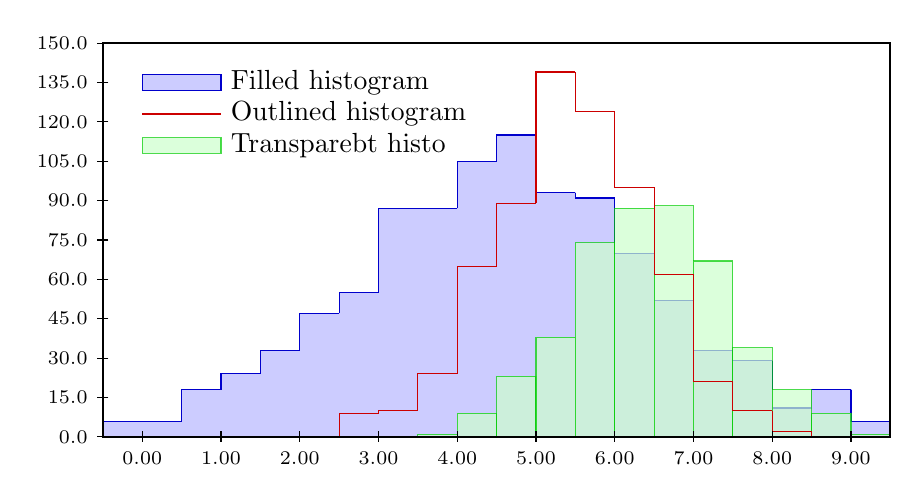
\begin{tikzpicture}
\begin{scope}[]
\clip (0,0) rectangle (10,5);
\begin{scope}[draw=blue!20,fill=blue!20]
\filldraw[] (0.0,0.0) -- (0.0,0.2) -- (0.5,0.2) -- (0.5,0.0);
\filldraw[] (0.5,0.0) -- (0.5,0.2) -- (1.0,0.2) -- (1.0,0.0);
\filldraw[] (1.0,0.0) -- (1.0,0.6) -- (1.5,0.6) -- (1.5,0.0);
\filldraw[] (1.5,0.0) -- (1.5,0.8) -- (2.0,0.8) -- (2.0,0.0);
\filldraw[] (2.0,0.0) -- (2.0,1.1) -- (2.5,1.1) -- (2.5,0.0);
\filldraw[] (2.5,0.0) -- (2.5,1.5666667) -- (3.0,1.5666667) -- (3.0,0.0);
\filldraw[] (3.0,0.0) -- (3.0,1.8333334) -- (3.5,1.8333334) -- (3.5,0.0);
\filldraw[] (3.5,0.0) -- (3.5,2.9) -- (4.0,2.9) -- (4.0,0.0);
\filldraw[] (4.0,0.0) -- (4.0,2.9) -- (4.5,2.9) -- (4.5,0.0);
\filldraw[] (4.5,0.0) -- (4.5,3.5) -- (5.0,3.5) -- (5.0,0.0);
\filldraw[] (5.0,0.0) -- (5.0,3.8333333) -- (5.5,3.8333333) -- (5.5,0.0);
\filldraw[] (5.5,0.0) -- (5.5,3.1) -- (6.0,3.1) -- (6.0,0.0);
\filldraw[] (6.0,0.0) -- (6.0,3.0333333) -- (6.5,3.0333333) -- (6.5,0.0);
\filldraw[] (6.5,0.0) -- (6.5,2.3333333) -- (7.0,2.3333333) -- (7.0,0.0);
\filldraw[] (7.0,0.0) -- (7.0,1.7333333) -- (7.5,1.7333333) -- (7.5,0.0);
\filldraw[] (7.5,0.0) -- (7.5,1.1) -- (8.0,1.1) -- (8.0,0.0);
\filldraw[] (8.0,0.0) -- (8.0,0.96666664) -- (8.5,0.96666664) -- (8.5,0.0);
\filldraw[] (8.5,0.0) -- (8.5,0.36666667) -- (9.0,0.36666667) -- (9.0,0.0);
\filldraw[] (9.0,0.0) -- (9.0,0.6) -- (9.5,0.6) -- (9.5,0.0);
\filldraw[] (9.5,0.0) -- (9.5,0.2) -- (10.0,0.2) -- (10.0,0.0);
\end{scope}
\begin{scope}[blue!80!black]
\draw[] (0.0,0.2) -- (0.5,0.2);
\draw (0.5,0.2) -- (0.5,0.2) -- (1.0,0.2);
\draw (1.0,0.2) -- (1.0,0.6) -- (1.5,0.6);
\draw (1.5,0.6) -- (1.5,0.8) -- (2.0,0.8);
\draw (2.0,0.8) -- (2.0,1.1) -- (2.5,1.1);
\draw (2.5,1.1) -- (2.5,1.5666667) -- (3.0,1.5666667);
\draw (3.0,1.5666667) -- (3.0,1.8333334) -- (3.5,1.8333334);
\draw (3.5,1.8333334) -- (3.5,2.9) -- (4.0,2.9);
\draw (4.0,2.9) -- (4.0,2.9) -- (4.5,2.9);
\draw (4.5,2.9) -- (4.5,3.5) -- (5.0,3.5);
\draw (5.0,3.5) -- (5.0,3.8333333) -- (5.5,3.8333333);
\draw (5.5,3.8333333) -- (5.5,3.1) -- (6.0,3.1);
\draw (6.0,3.1) -- (6.0,3.0333333) -- (6.5,3.0333333);
\draw (6.5,3.0333333) -- (6.5,2.3333333) -- (7.0,2.3333333);
\draw (7.0,2.3333333) -- (7.0,1.7333333) -- (7.5,1.7333333);
\draw (7.5,1.7333333) -- (7.5,1.1) -- (8.0,1.1);
\draw (8.0,1.1) -- (8.0,0.96666664) -- (8.5,0.96666664);
\draw (8.5,0.96666664) -- (8.5,0.36666667) -- (9.0,0.36666667);
\draw (9.0,0.36666667) -- (9.0,0.6) -- (9.5,0.6);
\draw (9.5,0.6) -- (9.5,0.2) -- (10.0,0.2);
\end{scope}
\begin{scope}[opacity=0.7,draw=green!80!black,fill=green!20]
\filldraw[] (0.0,0.0) -- (0.0,0.0) -- (0.5,0.0) -- (0.5,0.0);
\filldraw[] (0.5,0.0) -- (0.5,0.0) -- (1.0,0.0) -- (1.0,0.0);
\filldraw[] (1.0,0.0) -- (1.0,0.0) -- (1.5,0.0) -- (1.5,0.0);
\filldraw[] (1.5,0.0) -- (1.5,0.0) -- (2.0,0.0) -- (2.0,0.0);
\filldraw[] (2.0,0.0) -- (2.0,0.0) -- (2.5,0.0) -- (2.5,0.0);
\filldraw[] (2.5,0.0) -- (2.5,0.0) -- (3.0,0.0) -- (3.0,0.0);
\filldraw[] (3.0,0.0) -- (3.0,0.0) -- (3.5,0.0) -- (3.5,0.0);
\filldraw[] (3.5,0.0) -- (3.5,0.0) -- (4.0,0.0) -- (4.0,0.0);
\filldraw[] (4.0,0.0) -- (4.0,0.033333335) -- (4.5,0.033333335) -- (4.5,0.0);
\filldraw[] (4.5,0.0) -- (4.5,0.3) -- (5.0,0.3) -- (5.0,0.0);
\filldraw[] (5.0,0.0) -- (5.0,0.76666665) -- (5.5,0.76666665) -- (5.5,0.0);
\filldraw[] (5.5,0.0) -- (5.5,1.2666667) -- (6.0,1.2666667) -- (6.0,0.0);
\filldraw[] (6.0,0.0) -- (6.0,2.4666667) -- (6.5,2.4666667) -- (6.5,0.0);
\filldraw[] (6.5,0.0) -- (6.5,2.9) -- (7.0,2.9) -- (7.0,0.0);
\filldraw[] (7.0,0.0) -- (7.0,2.9333334) -- (7.5,2.9333334) -- (7.5,0.0);
\filldraw[] (7.5,0.0) -- (7.5,2.2333333) -- (8.0,2.2333333) -- (8.0,0.0);
\filldraw[] (8.0,0.0) -- (8.0,1.1333333) -- (8.5,1.1333333) -- (8.5,0.0);
\filldraw[] (8.5,0.0) -- (8.5,0.6) -- (9.0,0.6) -- (9.0,0.0);
\filldraw[] (9.0,0.0) -- (9.0,0.3) -- (9.5,0.3) -- (9.5,0.0);
\filldraw[] (9.5,0.0) -- (9.5,0.033333335) -- (10.0,0.033333335) -- (10.0,0.0);
\end{scope}
\begin{scope}[red!80!black]
\draw[] (0.0,0.0) -- (0.5,0.0);
\draw (0.5,0.0) -- (0.5,0.0) -- (1.0,0.0);
\draw (1.0,0.0) -- (1.0,0.0) -- (1.5,0.0);
\draw (1.5,0.0) -- (1.5,0.0) -- (2.0,0.0);
\draw (2.0,0.0) -- (2.0,0.0) -- (2.5,0.0);
\draw (2.5,0.0) -- (2.5,0.0) -- (3.0,0.0);
\draw (3.0,0.0) -- (3.0,0.3) -- (3.5,0.3);
\draw (3.5,0.3) -- (3.5,0.33333334) -- (4.0,0.33333334);
\draw (4.0,0.33333334) -- (4.0,0.8) -- (4.5,0.8);
\draw (4.5,0.8) -- (4.5,2.1666667) -- (5.0,2.1666667);
\draw (5.0,2.1666667) -- (5.0,2.9666667) -- (5.5,2.9666667);
\draw (5.5,2.9666667) -- (5.5,4.633333) -- (6.0,4.633333);
\draw (6.0,4.633333) -- (6.0,4.133333) -- (6.5,4.133333);
\draw (6.5,4.133333) -- (6.5,3.1666667) -- (7.0,3.1666667);
\draw (7.0,3.1666667) -- (7.0,2.0666666) -- (7.5,2.0666666);
\draw (7.5,2.0666666) -- (7.5,0.7) -- (8.0,0.7);
\draw (8.0,0.7) -- (8.0,0.33333334) -- (8.5,0.33333334);
\draw (8.5,0.33333334) -- (8.5,0.06666667) -- (9.0,0.06666667);
\draw (9.0,0.06666667) -- (9.0,0.0) -- (9.5,0.0);
\draw (9.5,0.0) -- (9.5,0.0) -- (10.0,0.0);
\end{scope}
\end{scope}
\draw (0.5,0cm + 2pt) -- (0.5, 0cm -2pt) node[below] {\scriptsize{\num[round-mode=places,round-precision=2]{0}}};
\draw (1.5,0cm + 2pt) -- (1.5, 0cm -2pt) node[below] {\scriptsize{\num[round-mode=places,round-precision=2]{1}}};
\draw (2.5,0cm + 2pt) -- (2.5, 0cm -2pt) node[below] {\scriptsize{\num[round-mode=places,round-precision=2]{2}}};
\draw (3.5,0cm + 2pt) -- (3.5, 0cm -2pt) node[below] {\scriptsize{\num[round-mode=places,round-precision=2]{3}}};
\draw (4.5,0cm + 2pt) -- (4.5, 0cm -2pt) node[below] {\scriptsize{\num[round-mode=places,round-precision=2]{4}}};
\draw (5.5,0cm + 2pt) -- (5.5, 0cm -2pt) node[below] {\scriptsize{\num[round-mode=places,round-precision=2]{5}}};
\draw (6.5,0cm + 2pt) -- (6.5, 0cm -2pt) node[below] {\scriptsize{\num[round-mode=places,round-precision=2]{6}}};
\draw (7.5,0cm + 2pt) -- (7.5, 0cm -2pt) node[below] {\scriptsize{\num[round-mode=places,round-precision=2]{7}}};
\draw (8.5,0cm + 2pt) -- (8.5, 0cm -2pt) node[below] {\scriptsize{\num[round-mode=places,round-precision=2]{8}}};
\draw (9.5,0cm + 2pt) -- (9.5, 0cm -2pt) node[below] {\scriptsize{\num[round-mode=places,round-precision=2]{9}}};
\draw (0cm + 2pt,0.    ) -- (0cm-2pt,0.    ) node[left] {\scriptsize{\num[round-mode=places,round-precision=1]{0}}};
\draw (0cm + 2pt,0.5    ) -- (0cm-2pt,0.5    ) node[left] {\scriptsize{\num[round-mode=places,round-precision=1]{15}}};
\draw (0cm + 2pt,1.    ) -- (0cm-2pt,1.    ) node[left] {\scriptsize{\num[round-mode=places,round-precision=1]{30}}};
\draw (0cm + 2pt,1.5    ) -- (0cm-2pt,1.5    ) node[left] {\scriptsize{\num[round-mode=places,round-precision=1]{45}}};
\draw (0cm + 2pt,2.    ) -- (0cm-2pt,2.    ) node[left] {\scriptsize{\num[round-mode=places,round-precision=1]{60}}};
\draw (0cm + 2pt,2.5    ) -- (0cm-2pt,2.5    ) node[left] {\scriptsize{\num[round-mode=places,round-precision=1]{75}}};
\draw (0cm + 2pt,3.    ) -- (0cm-2pt,3.    ) node[left] {\scriptsize{\num[round-mode=places,round-precision=1]{90}}};
\draw (0cm + 2pt,3.5    ) -- (0cm-2pt,3.5    ) node[left] {\scriptsize{\num[round-mode=places,round-precision=1]{105}}};
\draw (0cm + 2pt,4.    ) -- (0cm-2pt,4.    ) node[left] {\scriptsize{\num[round-mode=places,round-precision=1]{120}}};
\draw (0cm + 2pt,4.5    ) -- (0cm-2pt,4.5    ) node[left] {\scriptsize{\num[round-mode=places,round-precision=1]{135}}};
\draw (0cm + 2pt,5.    ) -- (0cm-2pt,5.    ) node[left] {\scriptsize{\num[round-mode=places,round-precision=1]{150}}};
\draw[thick] (0,0) rectangle (10,5);
\draw[draw=blue!20,fill=blue!20] (0.5,4.4) rectangle (1.5,4.6);
; 
\draw[blue!80!black] (0.5,4.4) rectangle (1.5,4.6);
; 
\node[right,] at (1.5,4.5) {Filled histogram};
\draw[red!80!black] (0.5,4.1) -- (1.5,4.1);
\node[right,] at (1.5,4.1) {Outlined histogram};
\draw[opacity=0.7,draw=green!80!black,fill=green!20] (0.5,3.6000001) rectangle (1.5,3.8);
; 
\node[right,] at (1.5,3.7) {Transparebt histo};
\end{tikzpicture}
%%% Local Variables: 
%%% mode: latex 
%%% TeX-master: "master" 
%%% End:


\captionsetup{singlelinecheck=off}
\caption[asdf]{Some Gaussian histograms with different styles and with legend entries. 
The legend entries are placed in the default cm frame, unless draw-histogram 
is called within (transform (tikz) ...). With some trickery it is also possible to get 
legends in captions: 
\begin{tikzpicture}[]
\begin{scope}[draw=gray,fill=blue!50]
\pgfpathmoveto{ \pgfpointxy {0.0} {0.0}}
\pgfpathlineto{ \pgfpointxy {0.4} {0.0}}
\pgfpathlineto{ \pgfpointxy {0.4} {0.2}}
\pgfpathlineto{ \pgfpointxy {0.0} {0.2}}
\pgfpathclose
\pgfusepath{ stroke, fill, }
\end{scope}
\end{tikzpicture}
 Histogram 1, \begin{tikzpicture}[]
\draw[red!80,thick] (0.0,0.1) -- (0.4,0.1);
\draw[opacity=0.0,white] (0.0,0.2) -- (0.0,0.0);
\end{tikzpicture}
 Histogram 2, 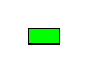
\begin{tikzpicture}[]
\begin{scope}[draw=black,fill=green]
\pgfpathmoveto{ \pgfpointxy {0.0} {0.0}}
\pgfpathlineto{ \pgfpointxy {0.4} {0.0}}
\pgfpathlineto{ \pgfpointxy {0.4} {0.2}}
\pgfpathlineto{ \pgfpointxy {0.0} {0.2}}
\pgfpathclose
\pgfusepath{ stroke, fill, }
\end{scope}
\end{tikzpicture}
 Histogram 3.}
\end{figure}


Simple sparkline: 
\begin{tikzpicture}[]
\begin{scope}[gray]
\begin{scope}[]
\pgfpathmoveto{ \pgfpointadd{\pgfpointxy {0.0} {0.0}} {\pgfpoint{0cm}{0cm}} }
\pgfpathlineto{ \pgfpointadd{\pgfpointxy {0.0} {0.0}} {\pgfpoint{3cm}{0cm}} }
\pgfpathlineto{ \pgfpointadd{\pgfpointxy {0.0} {0.0}} {\pgfpoint{3cm}{0.3cm}} }
\pgfpathlineto{ \pgfpointadd{\pgfpointxy {0.0} {0.0}} {\pgfpoint{0cm}{0.3cm}} }
\pgfpathclose
\pgfusepath{  clip, }
\begin{scope}[shift={(0.0,0.0)}]
\pgfsetxvec{\pgfpoint{0.6cm}{0cm}}
\pgfsetyvec{\pgfpoint{0cm}{0.003cm}}
\begin{scope}[shift={(0.0,0.0)}]
\pgfpathmoveto{ \pgfpointxy {0.024999999999999994} {0.0}}
\pgfpathlineto{ \pgfpointxy {0.225} {0.0}}
\pgfpathlineto{ \pgfpointxy {0.225} {4.0}}
\pgfpathlineto{ \pgfpointxy {0.024999999999999994} {4.0}}
\pgfpathclose
\pgfusepath{ stroke, fill, }
\pgfpathmoveto{ \pgfpointxy {0.275} {0.0}}
\pgfpathlineto{ \pgfpointxy {0.475} {0.0}}
\pgfpathlineto{ \pgfpointxy {0.475} {7.0}}
\pgfpathlineto{ \pgfpointxy {0.275} {7.0}}
\pgfpathclose
\pgfusepath{ stroke, fill, }
\pgfpathmoveto{ \pgfpointxy {0.525} {0.0}}
\pgfpathlineto{ \pgfpointxy {0.725} {0.0}}
\pgfpathlineto{ \pgfpointxy {0.725} {7.0}}
\pgfpathlineto{ \pgfpointxy {0.525} {7.0}}
\pgfpathclose
\pgfusepath{ stroke, fill, }
\pgfpathmoveto{ \pgfpointxy {0.775} {0.0}}
\pgfpathlineto{ \pgfpointxy {0.975} {0.0}}
\pgfpathlineto{ \pgfpointxy {0.975} {13.0}}
\pgfpathlineto{ \pgfpointxy {0.775} {13.0}}
\pgfpathclose
\pgfusepath{ stroke, fill, }
\pgfpathmoveto{ \pgfpointxy {1.025} {0.0}}
\pgfpathlineto{ \pgfpointxy {1.225} {0.0}}
\pgfpathlineto{ \pgfpointxy {1.225} {16.0}}
\pgfpathlineto{ \pgfpointxy {1.025} {16.0}}
\pgfpathclose
\pgfusepath{ stroke, fill, }
\pgfpathmoveto{ \pgfpointxy {1.275} {0.0}}
\pgfpathlineto{ \pgfpointxy {1.475} {0.0}}
\pgfpathlineto{ \pgfpointxy {1.475} {10.0}}
\pgfpathlineto{ \pgfpointxy {1.275} {10.0}}
\pgfpathclose
\pgfusepath{ stroke, fill, }
\pgfpathmoveto{ \pgfpointxy {1.525} {0.0}}
\pgfpathlineto{ \pgfpointxy {1.725} {0.0}}
\pgfpathlineto{ \pgfpointxy {1.725} {28.0}}
\pgfpathlineto{ \pgfpointxy {1.525} {28.0}}
\pgfpathclose
\pgfusepath{ stroke, fill, }
\pgfpathmoveto{ \pgfpointxy {1.775} {0.0}}
\pgfpathlineto{ \pgfpointxy {1.975} {0.0}}
\pgfpathlineto{ \pgfpointxy {1.975} {26.0}}
\pgfpathlineto{ \pgfpointxy {1.775} {26.0}}
\pgfpathclose
\pgfusepath{ stroke, fill, }
\pgfpathmoveto{ \pgfpointxy {2.025} {0.0}}
\pgfpathlineto{ \pgfpointxy {2.225} {0.0}}
\pgfpathlineto{ \pgfpointxy {2.225} {29.0}}
\pgfpathlineto{ \pgfpointxy {2.025} {29.0}}
\pgfpathclose
\pgfusepath{ stroke, fill, }
\pgfpathmoveto{ \pgfpointxy {2.275} {0.0}}
\pgfpathlineto{ \pgfpointxy {2.475} {0.0}}
\pgfpathlineto{ \pgfpointxy {2.475} {30.0}}
\pgfpathlineto{ \pgfpointxy {2.275} {30.0}}
\pgfpathclose
\pgfusepath{ stroke, fill, }
\pgfpathmoveto{ \pgfpointxy {2.525} {0.0}}
\pgfpathlineto{ \pgfpointxy {2.725} {0.0}}
\pgfpathlineto{ \pgfpointxy {2.725} {25.0}}
\pgfpathlineto{ \pgfpointxy {2.525} {25.0}}
\pgfpathclose
\pgfusepath{ stroke, fill, }
\pgfpathmoveto{ \pgfpointxy {2.775} {0.0}}
\pgfpathlineto{ \pgfpointxy {2.975} {0.0}}
\pgfpathlineto{ \pgfpointxy {2.975} {47.0}}
\pgfpathlineto{ \pgfpointxy {2.775} {47.0}}
\pgfpathclose
\pgfusepath{ stroke, fill, }
\pgfpathmoveto{ \pgfpointxy {3.025} {0.0}}
\pgfpathlineto{ \pgfpointxy {3.225} {0.0}}
\pgfpathlineto{ \pgfpointxy {3.225} {40.0}}
\pgfpathlineto{ \pgfpointxy {3.025} {40.0}}
\pgfpathclose
\pgfusepath{ stroke, fill, }
\pgfpathmoveto{ \pgfpointxy {3.275} {0.0}}
\pgfpathlineto{ \pgfpointxy {3.475} {0.0}}
\pgfpathlineto{ \pgfpointxy {3.475} {43.0}}
\pgfpathlineto{ \pgfpointxy {3.275} {43.0}}
\pgfpathclose
\pgfusepath{ stroke, fill, }
\pgfpathmoveto{ \pgfpointxy {3.525} {0.0}}
\pgfpathlineto{ \pgfpointxy {3.725} {0.0}}
\pgfpathlineto{ \pgfpointxy {3.725} {43.0}}
\pgfpathlineto{ \pgfpointxy {3.525} {43.0}}
\pgfpathclose
\pgfusepath{ stroke, fill, }
\pgfpathmoveto{ \pgfpointxy {3.775} {0.0}}
\pgfpathlineto{ \pgfpointxy {3.975} {0.0}}
\pgfpathlineto{ \pgfpointxy {3.975} {50.0}}
\pgfpathlineto{ \pgfpointxy {3.775} {50.0}}
\pgfpathclose
\pgfusepath{ stroke, fill, }
\pgfpathmoveto{ \pgfpointxy {4.025} {0.0}}
\pgfpathlineto{ \pgfpointxy {4.225} {0.0}}
\pgfpathlineto{ \pgfpointxy {4.225} {49.0}}
\pgfpathlineto{ \pgfpointxy {4.025} {49.0}}
\pgfpathclose
\pgfusepath{ stroke, fill, }
\pgfpathmoveto{ \pgfpointxy {4.275} {0.0}}
\pgfpathlineto{ \pgfpointxy {4.475} {0.0}}
\pgfpathlineto{ \pgfpointxy {4.475} {44.0}}
\pgfpathlineto{ \pgfpointxy {4.275} {44.0}}
\pgfpathclose
\pgfusepath{ stroke, fill, }
\pgfpathmoveto{ \pgfpointxy {4.525} {0.0}}
\pgfpathlineto{ \pgfpointxy {4.725} {0.0}}
\pgfpathlineto{ \pgfpointxy {4.725} {44.0}}
\pgfpathlineto{ \pgfpointxy {4.525} {44.0}}
\pgfpathclose
\pgfusepath{ stroke, fill, }
\pgfpathmoveto{ \pgfpointxy {4.775} {0.0}}
\pgfpathlineto{ \pgfpointxy {4.975} {0.0}}
\pgfpathlineto{ \pgfpointxy {4.975} {48.0}}
\pgfpathlineto{ \pgfpointxy {4.775} {48.0}}
\pgfpathclose
\pgfusepath{ stroke, fill, }
\end{scope}
\pgfsetxvec{\pgfpoint{1cm}{0cm}}
\pgfsetyvec{\pgfpoint{0cm}{1cm}}
\end{scope}
\end{scope}
\end{scope}
\end{tikzpicture}




More complex sparkline: 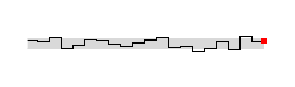
\begin{tikzpicture}[]
\begin{scope}[]
\pgfpathmoveto{ \pgfpointadd{\pgfpointxy {0.0} {0.0}} {\pgfpoint{0cm}{0cm}} }
\pgfpathlineto{ \pgfpointadd{\pgfpointxy {0.0} {0.0}} {\pgfpoint{3cm}{0cm}} }
\pgfpathlineto{ \pgfpointadd{\pgfpointxy {0.0} {0.0}} {\pgfpoint{3cm}{0.4cm}} }
\pgfpathlineto{ \pgfpointadd{\pgfpointxy {0.0} {0.0}} {\pgfpoint{0cm}{0.4cm}} }
\pgfpathclose
\pgfusepath{  clip, }
\begin{scope}[shift={(0.0,0.0)}]
\pgfsetxvec{\pgfpoint{0.30303030303030304cm}{0cm}}
\pgfsetyvec{\pgfpoint{0cm}{0.06666666666666667cm}}
\begin{scope}[shift={(-0.1,3.0)}]
\begin{scope}[gray!30]
\pgfpathmoveto{ \pgfpointxy {0.0} {-1.0}}
\pgfpathlineto{ \pgfpointxy {10.0} {-1.0}}
\pgfpathlineto{ \pgfpointxy {10.0} {1.0}}
\pgfpathlineto{ \pgfpointxy {0.0} {1.0}}
\pgfpathclose
\pgfusepath{ stroke, fill, }
\end{scope}
\end{scope}
\pgfsetxvec{\pgfpoint{1cm}{0cm}}
\pgfsetyvec{\pgfpoint{0cm}{1cm}}
\end{scope}
\end{scope}
\begin{scope}[]
\pgfpathmoveto{ \pgfpointadd{\pgfpointxy {0.0} {0.0}} {\pgfpoint{0cm}{0cm}} }
\pgfpathlineto{ \pgfpointadd{\pgfpointxy {0.0} {0.0}} {\pgfpoint{3cm}{0cm}} }
\pgfpathlineto{ \pgfpointadd{\pgfpointxy {0.0} {0.0}} {\pgfpoint{3cm}{0.4cm}} }
\pgfpathlineto{ \pgfpointadd{\pgfpointxy {0.0} {0.0}} {\pgfpoint{0cm}{0.4cm}} }
\pgfpathclose
\pgfusepath{  clip, }
\begin{scope}[shift={(0.0,0.0)}]
\pgfsetxvec{\pgfpoint{0.30303030303030304cm}{0cm}}
\pgfsetyvec{\pgfpoint{0cm}{0.06666666666666667cm}}
\begin{scope}[shift={(-0.1,3.0)}]
\begin{scope}[black]
\pgfpathmoveto{ \pgfpointxy {10.0} {0.0}}
\pgfpathlineto{ \pgfpointxy {10.0} {0.4120354243258191}}
\pgfpathlineto{ \pgfpointxy {10.0} {0.4120354243258191}}
\pgfpathlineto{ \pgfpointxy {9.5} {0.4120354243258191}}
\pgfpathlineto{ \pgfpointxy {9.5} {1.2972875032267412}}
\pgfpathlineto{ \pgfpointxy {9.0} {1.2972875032267412}}
\pgfpathlineto{ \pgfpointxy {9.0} {-1.1940949958777678}}
\pgfpathlineto{ \pgfpointxy {8.5} {-1.1940949958777678}}
\pgfpathlineto{ \pgfpointxy {8.5} {0.37196456919339244}}
\pgfpathlineto{ \pgfpointxy {8.0} {0.37196456919339244}}
\pgfpathlineto{ \pgfpointxy {8.0} {-0.8990533411219862}}
\pgfpathlineto{ \pgfpointxy {7.5} {-0.8990533411219862}}
\pgfpathlineto{ \pgfpointxy {7.5} {-1.4696141454200577}}
\pgfpathlineto{ \pgfpointxy {7.0} {-1.4696141454200577}}
\pgfpathlineto{ \pgfpointxy {7.0} {-0.6143147680500118}}
\pgfpathlineto{ \pgfpointxy {6.5} {-0.6143147680500118}}
\pgfpathlineto{ \pgfpointxy {6.5} {-0.8120266156699267}}
\pgfpathlineto{ \pgfpointxy {6.0} {-0.8120266156699267}}
\pgfpathlineto{ \pgfpointxy {6.0} {1.1952488728650348}}
\pgfpathlineto{ \pgfpointxy {5.5} {1.1952488728650348}}
\pgfpathlineto{ \pgfpointxy {5.5} {0.6578528417618186}}
\pgfpathlineto{ \pgfpointxy {5.0} {0.6578528417618186}}
\pgfpathlineto{ \pgfpointxy {5.0} {0.07274063155103876}}
\pgfpathlineto{ \pgfpointxy {4.5} {0.07274063155103876}}
\pgfpathlineto{ \pgfpointxy {4.5} {-0.6455046593749983}}
\pgfpathlineto{ \pgfpointxy {4.0} {-0.6455046593749983}}
\pgfpathlineto{ \pgfpointxy {4.0} {-0.13443197412707805}}
\pgfpathlineto{ \pgfpointxy {3.5} {-0.13443197412707805}}
\pgfpathlineto{ \pgfpointxy {3.5} {0.5949379106277703}}
\pgfpathlineto{ \pgfpointxy {3.0} {0.5949379106277703}}
\pgfpathlineto{ \pgfpointxy {3.0} {0.7116482481345028}}
\pgfpathlineto{ \pgfpointxy {2.5} {0.7116482481345028}}
\pgfpathlineto{ \pgfpointxy {2.5} {-0.3289483999491816}}
\pgfpathlineto{ \pgfpointxy {2.0} {-0.3289483999491816}}
\pgfpathlineto{ \pgfpointxy {2.0} {-0.9084599432524058}}
\pgfpathlineto{ \pgfpointxy {1.5} {-0.9084599432524058}}
\pgfpathlineto{ \pgfpointxy {1.5} {1.0665272321859438}}
\pgfpathlineto{ \pgfpointxy {1.0} {1.0665272321859438}}
\pgfpathlineto{ \pgfpointxy {1.0} {0.3664309495225071}}
\pgfpathlineto{ \pgfpointxy {0.5} {0.3664309495225071}}
\pgfpathlineto{ \pgfpointxy {0.5} {0.5870575582846191}}
\pgfpathlineto{ \pgfpointxy {0.0} {0.5870575582846191}}
\pgfpathlineto{ \pgfpointxy {0.0} {0.0}}
\pgfusepath{ stroke, }
\end{scope}
\end{scope}
\pgfsetxvec{\pgfpoint{1cm}{0cm}}
\pgfsetyvec{\pgfpoint{0cm}{1cm}}
\end{scope}
\end{scope}
\begin{scope}[shift={(0.0,0.0)}]
\pgfsetxvec{\pgfpoint{0.30303030303030304cm}{0cm}}
\pgfsetyvec{\pgfpoint{0cm}{0.06666666666666667cm}}
\begin{scope}[shift={(-0.1,3.0)}]
\node at (10.0,0.4120354243258191) [red,fill=red,rectangle,inner sep=0.0pt,minimum width =2.0pt,minimum height=2.0pt] {};
\end{scope}
\pgfsetxvec{\pgfpoint{1cm}{0cm}}
\pgfsetyvec{\pgfpoint{0cm}{1cm}}
\end{scope}
\end{tikzpicture}
 \textcolor{red}{ 0.4}, 
\begin{tikzpicture}[]
\begin{scope}[draw=gray!30,fill=gray!30]
\pgfpathmoveto{ \pgfpointxy {0.0} {0.0}}
\pgfpathlineto{ \pgfpointxy {0.4} {0.0}}
\pgfpathlineto{ \pgfpointxy {0.4} {0.2}}
\pgfpathlineto{ \pgfpointxy {0.0} {0.2}}
\pgfpathclose
\pgfusepath{ stroke, fill, }
\end{scope}
\end{tikzpicture}
 indicates the $1 \sigma$ band

\begin{figure}[H]
\centering
\input{/home/haavagj/src/tikz-helper/example/test-histo3.tex}
\captionsetup{singlelinecheck=off}
\caption[asdf]{Histogram with bins extending in the horizontal direction. 
This is just a tikzpicture with the transformation rotate=-90. The text is not rotated, so axis ticks
require extra care, and text in legend entries will not be properly aligned.
The bins are named with the draw-axis-ticks function.}
\end{figure}
\begin{figure}[H]
\centering
%%% AUTO GENERATED CODE
\documentclass{standalone}
\ifx\HCode\UnDef\else\def\pgfsysdriver{pgfsys-tex4ht.def}\fi
\usepackage[usenames,dvipsnames,svgnames,table]{xcolor}
\usepackage{tikz}
\usepackage{color}
\usepackage{siunitx}
\usetikzlibrary{arrows,shapes}
\begin{document}
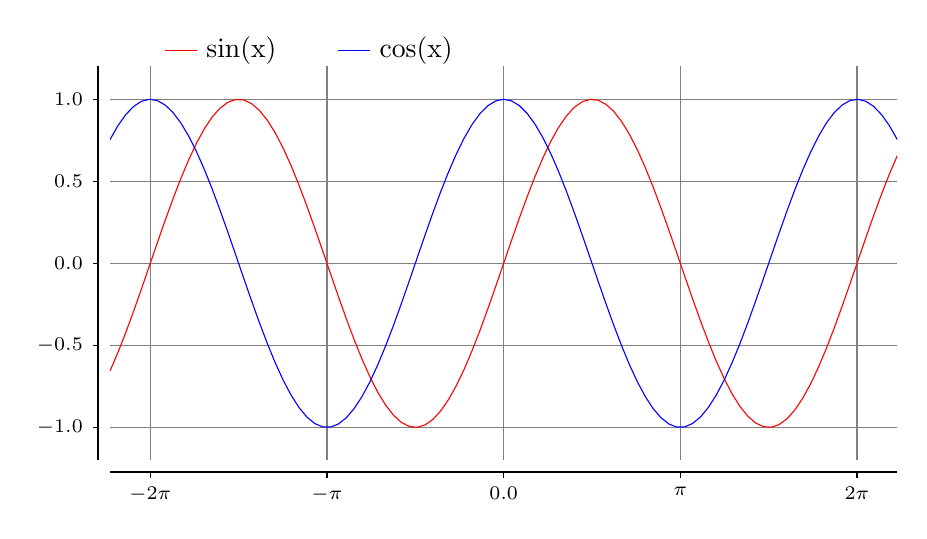
\begin{tikzpicture}
\begin{scope}[shift={(0.0,0.0)}]
\pgfsetxvec{\pgfpoint{0.71428573cm}{0cm}}
\pgfsetyvec{\pgfpoint{0cm}{2.0833333cm}}
\begin{scope}[shift={(7.0,1.2)}]
\begin{scope}[thin,gray]
\pgfpathmoveto{ \pgfpointxy {-6.283185307179586} {-1.2}}
\pgfpathlineto{ \pgfpointxy {-6.283185307179586} {1.2}}
\pgfpathmoveto{ \pgfpointxy {-3.141592653589793} {-1.2}}
\pgfpathlineto{ \pgfpointxy {-3.141592653589793} {1.2}}
\pgfpathmoveto{ \pgfpointxy {0.0} {-1.2}}
\pgfpathlineto{ \pgfpointxy {0.0} {1.2}}
\pgfpathmoveto{ \pgfpointxy {3.141592653589793} {-1.2}}
\pgfpathlineto{ \pgfpointxy {3.141592653589793} {1.2}}
\pgfpathmoveto{ \pgfpointxy {6.283185307179586} {-1.2}}
\pgfpathlineto{ \pgfpointxy {6.283185307179586} {1.2}}
\pgfpathmoveto{ \pgfpointxy {-7.0} {-1.0}}
\pgfpathlineto{ \pgfpointxy {7.0} {-1.0}}
\pgfpathmoveto{ \pgfpointxy {-7.0} {-0.5}}
\pgfpathlineto{ \pgfpointxy {7.0} {-0.5}}
\pgfpathmoveto{ \pgfpointxy {-7.0} {0.0}}
\pgfpathlineto{ \pgfpointxy {7.0} {0.0}}
\pgfpathmoveto{ \pgfpointxy {-7.0} {0.5}}
\pgfpathlineto{ \pgfpointxy {7.0} {0.5}}
\pgfpathmoveto{ \pgfpointxy {-7.0} {1.0}}
\pgfpathlineto{ \pgfpointxy {7.0} {1.0}}
\pgfusepath{ stroke, }
\end{scope}
\end{scope}
\pgfsetxvec{\pgfpoint{1cm}{0cm}}
\pgfsetyvec{\pgfpoint{0cm}{1cm}}
\end{scope}
\begin{scope}[shift={(0.0,0.0)}]
\pgfsetxvec{\pgfpoint{0.71428573cm}{0cm}}
\pgfsetyvec{\pgfpoint{0cm}{2.0833333cm}}
\begin{scope}[shift={(7.0,1.2)}]
\begin{scope}[thick,black,fill=white]
\pgfpathmoveto{ \pgfpointadd{\pgfpointxy {-7.0} {-1.2}} {\pgfpoint{0}{-0.15cm}} }
\pgfpathlineto{ \pgfpointadd{\pgfpointxy {7.0} {-1.2}} {\pgfpoint{0}{-0.15cm}} }
\pgfpathmoveto{ \pgfpointadd{\pgfpointxy {-7.0} {-1.2}} {\pgfpoint{-0.15cm}{0}} }
\pgfpathlineto{ \pgfpointadd{\pgfpointxy {-7.0} {1.2}} {\pgfpoint{-0.15cm}{0}} }
\pgfusepath{ stroke, }
\end{scope}
\begin{scope}[yshift=-0.15cm]
\draw[] [shift={(-6.283185307179586,-1.2)}] (0,0) -- (0,-2pt) node[below]{ \scriptsize{$-2\pi$}};
\draw[] [shift={(-3.141592653589793,-1.2)}] (0,0) -- (0,-2pt) node[below]{ \scriptsize{$-\pi$}};
\draw[] [shift={(0.0,-1.2)}] (0,0) -- (0,-2pt) node[below]{ \scriptsize{0.0}};
\draw[] [shift={(3.141592653589793,-1.2)}] (0,0) -- (0,-2pt) node[below]{ \scriptsize{$\pi$}};
\draw[] [shift={(6.283185307179586,-1.2)}] (0,0) -- (0,-2pt) node[below]{ \scriptsize{$2\pi$}};
\end{scope}
\begin{scope}[xshift=-0.15cm]
\draw[] [shift={(-7.0,-1.0)}] (0,0) -- (-2pt,0) node[left]{ \scriptsize{\num[round-mode=places,round-precision=1]{-1.0}}};
\draw[] [shift={(-7.0,-0.5)}] (0,0) -- (-2pt,0) node[left]{ \scriptsize{\num[round-mode=places,round-precision=1]{-0.5}}};
\draw[] [shift={(-7.0,0.0)}] (0,0) -- (-2pt,0) node[left]{ \scriptsize{\num[round-mode=places,round-precision=1]{0.0}}};
\draw[] [shift={(-7.0,0.5)}] (0,0) -- (-2pt,0) node[left]{ \scriptsize{\num[round-mode=places,round-precision=1]{0.5}}};
\draw[] [shift={(-7.0,1.0)}] (0,0) -- (-2pt,0) node[left]{ \scriptsize{\num[round-mode=places,round-precision=1]{1.0}}};
\end{scope}
\end{scope}
\pgfsetxvec{\pgfpoint{1cm}{0cm}}
\pgfsetyvec{\pgfpoint{0cm}{1cm}}
\end{scope}
\begin{scope}[]
\pgfpathmoveto{ \pgfpointadd{\pgfpointxy {0.0} {0.0}} {\pgfpoint{0cm}{0cm}} }
\pgfpathlineto{ \pgfpointadd{\pgfpointxy {0.0} {0.0}} {\pgfpoint{10cm}{0cm}} }
\pgfpathlineto{ \pgfpointadd{\pgfpointxy {0.0} {0.0}} {\pgfpoint{10cm}{5cm}} }
\pgfpathlineto{ \pgfpointadd{\pgfpointxy {0.0} {0.0}} {\pgfpoint{0cm}{5cm}} }
\pgfpathclose
\pgfusepath{  clip, }
\begin{scope}[shift={(0.0,0.0)}]
\pgfsetxvec{\pgfpoint{0.71428573cm}{0cm}}
\pgfsetyvec{\pgfpoint{0cm}{2.0833333cm}}
\begin{scope}[shift={(7.0,1.2)}]
\begin{scope}[red]
\pgfpathmoveto{ \pgfpointxy {-7.0} {-0.6569866}}
\pgfpathlineto{ \pgfpointxy {-6.86} {-0.54535675}}
\pgfpathlineto{ \pgfpointxy {-6.72} {-0.4230554}}
\pgfpathlineto{ \pgfpointxy {-6.58} {-0.29247567}}
\pgfpathlineto{ \pgfpointxy {-6.44} {-0.15617278}}
\pgfpathlineto{ \pgfpointxy {-6.3} {-0.0168139}}
\pgfpathlineto{ \pgfpointxy {-6.16} {0.12287399}}
\pgfpathlineto{ \pgfpointxy {-6.02} {0.2601575}}
\pgfpathlineto{ \pgfpointxy {-5.88} {0.39235023}}
\pgfpathlineto{ \pgfpointxy {-5.74} {0.51686543}}
\pgfpathlineto{ \pgfpointxy {-5.6} {0.63126665}}
\pgfpathlineto{ \pgfpointxy {-5.46} {0.7333152}}
\pgfpathlineto{ \pgfpointxy {-5.32} {0.8210142}}
\pgfpathlineto{ \pgfpointxy {-5.18} {0.8926477}}
\pgfpathlineto{ \pgfpointxy {-5.04} {0.94681376}}
\pgfpathlineto{ \pgfpointxy {-4.9} {0.98245263}}
\pgfpathlineto{ \pgfpointxy {-4.76} {0.9988668}}
\pgfpathlineto{ \pgfpointxy {-4.62} {0.99573517}}
\pgfpathlineto{ \pgfpointxy {-4.48} {0.97311896}}
\pgfpathlineto{ \pgfpointxy {-4.34} {0.9314608}}
\pgfpathlineto{ \pgfpointxy {-4.2} {0.8715758}}
\pgfpathlineto{ \pgfpointxy {-4.06} {0.7946358}}
\pgfpathlineto{ \pgfpointxy {-3.92} {0.7021463}}
\pgfpathlineto{ \pgfpointxy {-3.78} {0.5959172}}
\pgfpathlineto{ \pgfpointxy {-3.64} {0.47802725}}
\pgfpathlineto{ \pgfpointxy {-3.5} {0.35078323}}
\pgfpathlineto{ \pgfpointxy {-3.36} {0.21667509}}
\pgfpathlineto{ \pgfpointxy {-3.22} {0.07832703}}
\pgfpathlineto{ \pgfpointxy {-3.08} {-0.061553717}}
\pgfpathlineto{ \pgfpointxy {-2.94} {-0.20022999}}
\pgfpathlineto{ \pgfpointxy {-2.8} {-0.33498815}}
\pgfpathlineto{ \pgfpointxy {-2.66} {-0.46319127}}
\pgfpathlineto{ \pgfpointxy {-2.52} {-0.58233064}}
\pgfpathlineto{ \pgfpointxy {-2.38} {-0.690075}}
\pgfpathlineto{ \pgfpointxy {-2.24} {-0.78431594}}
\pgfpathlineto{ \pgfpointxy {-2.1} {-0.86320937}}
\pgfpathlineto{ \pgfpointxy {-1.96} {-0.92521155}}
\pgfpathlineto{ \pgfpointxy {-1.82} {-0.9691091}}
\pgfpathlineto{ \pgfpointxy {-1.68} {-0.99404323}}
\pgfpathlineto{ \pgfpointxy {-1.54} {-0.99952585}}
\pgfpathlineto{ \pgfpointxy {-1.4} {-0.98544973}}
\pgfpathlineto{ \pgfpointxy {-1.26} {-0.9520903}}
\pgfpathlineto{ \pgfpointxy {-1.12} {-0.90010047}}
\pgfpathlineto{ \pgfpointxy {-0.98} {-0.8304974}}
\pgfpathlineto{ \pgfpointxy {-0.84} {-0.7446431}}
\pgfpathlineto{ \pgfpointxy {-0.7} {-0.64421767}}
\pgfpathlineto{ \pgfpointxy {-0.56} {-0.5311862}}
\pgfpathlineto{ \pgfpointxy {-0.42} {-0.40776044}}
\pgfpathlineto{ \pgfpointxy {-0.28} {-0.27635565}}
\pgfpathlineto{ \pgfpointxy {-0.14} {-0.13954312}}
\pgfpathlineto{ \pgfpointxy {0.0} {0.0}}
\pgfpathlineto{ \pgfpointxy {0.14} {0.13954312}}
\pgfpathlineto{ \pgfpointxy {0.28} {0.27635565}}
\pgfpathlineto{ \pgfpointxy {0.42} {0.40776044}}
\pgfpathlineto{ \pgfpointxy {0.56} {0.5311862}}
\pgfpathlineto{ \pgfpointxy {0.7} {0.64421767}}
\pgfpathlineto{ \pgfpointxy {0.84} {0.7446431}}
\pgfpathlineto{ \pgfpointxy {0.98} {0.8304974}}
\pgfpathlineto{ \pgfpointxy {1.12} {0.90010047}}
\pgfpathlineto{ \pgfpointxy {1.26} {0.9520903}}
\pgfpathlineto{ \pgfpointxy {1.4} {0.98544973}}
\pgfpathlineto{ \pgfpointxy {1.54} {0.99952585}}
\pgfpathlineto{ \pgfpointxy {1.68} {0.99404323}}
\pgfpathlineto{ \pgfpointxy {1.82} {0.9691091}}
\pgfpathlineto{ \pgfpointxy {1.96} {0.92521155}}
\pgfpathlineto{ \pgfpointxy {2.1} {0.86320937}}
\pgfpathlineto{ \pgfpointxy {2.24} {0.78431594}}
\pgfpathlineto{ \pgfpointxy {2.38} {0.690075}}
\pgfpathlineto{ \pgfpointxy {2.52} {0.58233064}}
\pgfpathlineto{ \pgfpointxy {2.66} {0.46319127}}
\pgfpathlineto{ \pgfpointxy {2.8} {0.33498815}}
\pgfpathlineto{ \pgfpointxy {2.94} {0.20022999}}
\pgfpathlineto{ \pgfpointxy {3.08} {0.061553717}}
\pgfpathlineto{ \pgfpointxy {3.22} {-0.07832703}}
\pgfpathlineto{ \pgfpointxy {3.36} {-0.21667509}}
\pgfpathlineto{ \pgfpointxy {3.5} {-0.35078323}}
\pgfpathlineto{ \pgfpointxy {3.64} {-0.47802725}}
\pgfpathlineto{ \pgfpointxy {3.78} {-0.5959172}}
\pgfpathlineto{ \pgfpointxy {3.92} {-0.7021463}}
\pgfpathlineto{ \pgfpointxy {4.06} {-0.7946358}}
\pgfpathlineto{ \pgfpointxy {4.2} {-0.8715758}}
\pgfpathlineto{ \pgfpointxy {4.34} {-0.9314608}}
\pgfpathlineto{ \pgfpointxy {4.48} {-0.97311896}}
\pgfpathlineto{ \pgfpointxy {4.62} {-0.99573517}}
\pgfpathlineto{ \pgfpointxy {4.76} {-0.9988668}}
\pgfpathlineto{ \pgfpointxy {4.9} {-0.98245263}}
\pgfpathlineto{ \pgfpointxy {5.04} {-0.94681376}}
\pgfpathlineto{ \pgfpointxy {5.18} {-0.8926477}}
\pgfpathlineto{ \pgfpointxy {5.32} {-0.8210142}}
\pgfpathlineto{ \pgfpointxy {5.46} {-0.7333152}}
\pgfpathlineto{ \pgfpointxy {5.6} {-0.63126665}}
\pgfpathlineto{ \pgfpointxy {5.74} {-0.51686543}}
\pgfpathlineto{ \pgfpointxy {5.88} {-0.39235023}}
\pgfpathlineto{ \pgfpointxy {6.02} {-0.2601575}}
\pgfpathlineto{ \pgfpointxy {6.16} {-0.12287399}}
\pgfpathlineto{ \pgfpointxy {6.3} {0.0168139}}
\pgfpathlineto{ \pgfpointxy {6.44} {0.15617278}}
\pgfpathlineto{ \pgfpointxy {6.58} {0.29247567}}
\pgfpathlineto{ \pgfpointxy {6.72} {0.4230554}}
\pgfpathlineto{ \pgfpointxy {6.86} {0.54535675}}
\pgfpathlineto{ \pgfpointxy {7.0} {0.6569866}}
\pgfusepath{ stroke, }
\end{scope}
\end{scope}
\pgfsetxvec{\pgfpoint{1cm}{0cm}}
\pgfsetyvec{\pgfpoint{0cm}{1cm}}
\end{scope}
\end{scope}
\draw[red] (0.7,5.2) -- (1.1,5.2);
\node at (1.1,5.2) [right,,] {sin(x)};
\begin{scope}[]
\pgfpathmoveto{ \pgfpointadd{\pgfpointxy {0.0} {0.0}} {\pgfpoint{0cm}{0cm}} }
\pgfpathlineto{ \pgfpointadd{\pgfpointxy {0.0} {0.0}} {\pgfpoint{10cm}{0cm}} }
\pgfpathlineto{ \pgfpointadd{\pgfpointxy {0.0} {0.0}} {\pgfpoint{10cm}{5cm}} }
\pgfpathlineto{ \pgfpointadd{\pgfpointxy {0.0} {0.0}} {\pgfpoint{0cm}{5cm}} }
\pgfpathclose
\pgfusepath{  clip, }
\begin{scope}[shift={(0.0,0.0)}]
\pgfsetxvec{\pgfpoint{0.71428573cm}{0cm}}
\pgfsetyvec{\pgfpoint{0cm}{2.0833333cm}}
\begin{scope}[shift={(7.0,1.2)}]
\begin{scope}[blue]
\pgfpathmoveto{ \pgfpointxy {-7.0} {0.75390226}}
\pgfpathlineto{ \pgfpointxy {-6.86} {0.838204}}
\pgfpathlineto{ \pgfpointxy {-6.72} {0.9061038}}
\pgfpathlineto{ \pgfpointxy {-6.58} {0.95627296}}
\pgfpathlineto{ \pgfpointxy {-6.44} {0.9877297}}
\pgfpathlineto{ \pgfpointxy {-6.3} {0.9998586}}
\pgfpathlineto{ \pgfpointxy {-6.16} {0.9924223}}
\pgfpathlineto{ \pgfpointxy {-6.02} {0.9655662}}
\pgfpathlineto{ \pgfpointxy {-5.88} {0.9198159}}
\pgfpathlineto{ \pgfpointxy {-5.74} {0.85606664}}
\pgfpathlineto{ \pgfpointxy {-5.6} {0.77556586}}
\pgfpathlineto{ \pgfpointxy {-5.46} {0.67988884}}
\pgfpathlineto{ \pgfpointxy {-5.32} {0.5709077}}
\pgfpathlineto{ \pgfpointxy {-5.18} {0.45075506}}
\pgfpathlineto{ \pgfpointxy {-5.04} {0.32178202}}
\pgfpathlineto{ \pgfpointxy {-4.9} {0.18651237}}
\pgfpathlineto{ \pgfpointxy {-4.76} {0.047593035}}
\pgfpathlineto{ \pgfpointxy {-4.62} {-0.092257604}}
\pgfpathlineto{ \pgfpointxy {-4.48} {-0.23030294}}
\pgfpathlineto{ \pgfpointxy {-4.34} {-0.3638417}}
\pgfpathlineto{ \pgfpointxy {-4.2} {-0.4902608}}
\pgfpathlineto{ \pgfpointxy {-4.06} {-0.6070865}}
\pgfpathlineto{ \pgfpointxy {-3.92} {-0.71203274}}
\pgfpathlineto{ \pgfpointxy {-3.78} {-0.80304587}}
\pgfpathlineto{ \pgfpointxy {-3.64} {-0.878345}}
\pgfpathlineto{ \pgfpointxy {-3.5} {-0.9364567}}
\pgfpathlineto{ \pgfpointxy {-3.36} {-0.9762438}}
\pgfpathlineto{ \pgfpointxy {-3.22} {-0.99692774}}
\pgfpathlineto{ \pgfpointxy {-3.08} {-0.9981038}}
\pgfpathlineto{ \pgfpointxy {-2.94} {-0.9797489}}
\pgfpathlineto{ \pgfpointxy {-2.8} {-0.94222236}}
\pgfpathlineto{ \pgfpointxy {-2.66} {-0.88625836}}
\pgfpathlineto{ \pgfpointxy {-2.52} {-0.81295204}}
\pgfpathlineto{ \pgfpointxy {-2.38} {-0.7237379}}
\pgfpathlineto{ \pgfpointxy {-2.24} {-0.6203616}}
\pgfpathlineto{ \pgfpointxy {-2.1} {-0.5048461}}
\pgfpathlineto{ \pgfpointxy {-1.96} {-0.37945175}}
\pgfpathlineto{ \pgfpointxy {-1.82} {-0.24663231}}
\pgfpathlineto{ \pgfpointxy {-1.68} {-0.10898675}}
\pgfpathlineto{ \pgfpointxy {-1.54} {0.03079146}}
\pgfpathlineto{ \pgfpointxy {-1.4} {0.16996714}}
\pgfpathlineto{ \pgfpointxy {-1.26} {0.30581692}}
\pgfpathlineto{ \pgfpointxy {-1.12} {0.43568245}}
\pgfpathlineto{ \pgfpointxy {-0.98} {0.5570226}}
\pgfpathlineto{ \pgfpointxy {-0.84} {0.6674628}}
\pgfpathlineto{ \pgfpointxy {-0.7} {0.7648422}}
\pgfpathlineto{ \pgfpointxy {-0.56} {0.8472551}}
\pgfpathlineto{ \pgfpointxy {-0.42} {0.9130889}}
\pgfpathlineto{ \pgfpointxy {-0.28} {0.96105546}}
\pgfpathlineto{ \pgfpointxy {-0.14} {0.990216}}
\pgfpathlineto{ \pgfpointxy {0.0} {1.0}}
\pgfpathlineto{ \pgfpointxy {0.14} {0.990216}}
\pgfpathlineto{ \pgfpointxy {0.28} {0.96105546}}
\pgfpathlineto{ \pgfpointxy {0.42} {0.9130889}}
\pgfpathlineto{ \pgfpointxy {0.56} {0.8472551}}
\pgfpathlineto{ \pgfpointxy {0.7} {0.7648422}}
\pgfpathlineto{ \pgfpointxy {0.84} {0.6674628}}
\pgfpathlineto{ \pgfpointxy {0.98} {0.5570226}}
\pgfpathlineto{ \pgfpointxy {1.12} {0.43568245}}
\pgfpathlineto{ \pgfpointxy {1.26} {0.30581692}}
\pgfpathlineto{ \pgfpointxy {1.4} {0.16996714}}
\pgfpathlineto{ \pgfpointxy {1.54} {0.03079146}}
\pgfpathlineto{ \pgfpointxy {1.68} {-0.10898675}}
\pgfpathlineto{ \pgfpointxy {1.82} {-0.24663231}}
\pgfpathlineto{ \pgfpointxy {1.96} {-0.37945175}}
\pgfpathlineto{ \pgfpointxy {2.1} {-0.5048461}}
\pgfpathlineto{ \pgfpointxy {2.24} {-0.6203616}}
\pgfpathlineto{ \pgfpointxy {2.38} {-0.7237379}}
\pgfpathlineto{ \pgfpointxy {2.52} {-0.81295204}}
\pgfpathlineto{ \pgfpointxy {2.66} {-0.88625836}}
\pgfpathlineto{ \pgfpointxy {2.8} {-0.94222236}}
\pgfpathlineto{ \pgfpointxy {2.94} {-0.9797489}}
\pgfpathlineto{ \pgfpointxy {3.08} {-0.9981038}}
\pgfpathlineto{ \pgfpointxy {3.22} {-0.99692774}}
\pgfpathlineto{ \pgfpointxy {3.36} {-0.9762438}}
\pgfpathlineto{ \pgfpointxy {3.5} {-0.9364567}}
\pgfpathlineto{ \pgfpointxy {3.64} {-0.878345}}
\pgfpathlineto{ \pgfpointxy {3.78} {-0.80304587}}
\pgfpathlineto{ \pgfpointxy {3.92} {-0.71203274}}
\pgfpathlineto{ \pgfpointxy {4.06} {-0.6070865}}
\pgfpathlineto{ \pgfpointxy {4.2} {-0.4902608}}
\pgfpathlineto{ \pgfpointxy {4.34} {-0.3638417}}
\pgfpathlineto{ \pgfpointxy {4.48} {-0.23030294}}
\pgfpathlineto{ \pgfpointxy {4.62} {-0.092257604}}
\pgfpathlineto{ \pgfpointxy {4.76} {0.047593035}}
\pgfpathlineto{ \pgfpointxy {4.9} {0.18651237}}
\pgfpathlineto{ \pgfpointxy {5.04} {0.32178202}}
\pgfpathlineto{ \pgfpointxy {5.18} {0.45075506}}
\pgfpathlineto{ \pgfpointxy {5.32} {0.5709077}}
\pgfpathlineto{ \pgfpointxy {5.46} {0.67988884}}
\pgfpathlineto{ \pgfpointxy {5.6} {0.77556586}}
\pgfpathlineto{ \pgfpointxy {5.74} {0.85606664}}
\pgfpathlineto{ \pgfpointxy {5.88} {0.9198159}}
\pgfpathlineto{ \pgfpointxy {6.02} {0.9655662}}
\pgfpathlineto{ \pgfpointxy {6.16} {0.9924223}}
\pgfpathlineto{ \pgfpointxy {6.3} {0.9998586}}
\pgfpathlineto{ \pgfpointxy {6.44} {0.9877297}}
\pgfpathlineto{ \pgfpointxy {6.58} {0.95627296}}
\pgfpathlineto{ \pgfpointxy {6.72} {0.9061038}}
\pgfpathlineto{ \pgfpointxy {6.86} {0.838204}}
\pgfpathlineto{ \pgfpointxy {7.0} {0.75390226}}
\pgfusepath{ stroke, }
\end{scope}
\end{scope}
\pgfsetxvec{\pgfpoint{1cm}{0cm}}
\pgfsetyvec{\pgfpoint{0cm}{1cm}}
\end{scope}
\end{scope}
\draw[blue] (2.9,5.2) -- (3.3000002,5.2);
\node at (3.3000002,5.2) [right,,] {cos(x)};
\end{tikzpicture}
\end{document}

\captionsetup{singlelinecheck=off}
\caption[asdf]{Plotting sin(x) and cos(x), with grid lines and tick names on the x-axis.}
\end{figure}
\begin{figure}[H]
\centering
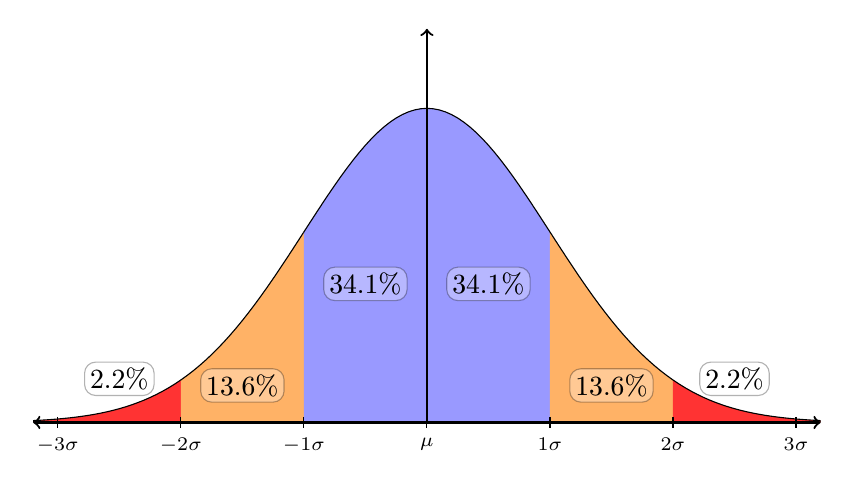
\begin{tikzpicture}[]
\begin{scope}[]
\clip (0,0) rectangle (10,5);
\begin{scope}[shift={(5.0,-0.0)}]
\pgfsetxvec{\pgfpoint{1.5625cm}{0cm}}
\pgfsetyvec{\pgfpoint{0cm}{10.0cm}}
\begin{scope}[]
\clip (-3.5,0) rectangle (-2,5);
\begin{scope}[fill=red!80]
\pgfpathmoveto{ \pgfqpointxy {-3.2} {0.0}}
\pgfpathlineto{ \pgfqpointxy {-3.2} {0.0023840873753184963}}
\pgfpathlineto{ \pgfqpointxy {-3.15} {0.002794257593560257}}
\pgfpathlineto{ \pgfqpointxy {-3.1000001} {0.0032668180294884892}}
\pgfpathlineto{ \pgfqpointxy {-3.05} {0.0038097626369961333}}
\pgfpathlineto{ \pgfqpointxy {-3.0} {0.004431848335480958}}
\pgfpathlineto{ \pgfqpointxy {-2.95} {0.005142640152435692}}
\pgfpathlineto{ \pgfqpointxy {-2.9} {0.0059525301721895674}}
\pgfpathlineto{ \pgfqpointxy {-2.8500001} {0.006872765030160735}}
\pgfpathlineto{ \pgfqpointxy {-2.8} {0.007915452600647405}}
\pgfpathlineto{ \pgfqpointxy {-2.75} {0.009093562739915748}}
\pgfpathlineto{ \pgfqpointxy {-2.7} {0.010420932487815211}}
\pgfpathlineto{ \pgfqpointxy {-2.65} {0.011912240802789813}}
\pgfpathlineto{ \pgfqpointxy {-2.6} {0.013582973636746678}}
\pgfpathlineto{ \pgfqpointxy {-2.55} {0.0154493503693536}}
\pgfpathlineto{ \pgfqpointxy {-2.5} {0.017528300772314036}}
\pgfpathlineto{ \pgfqpointxy {-2.45} {0.01983735428926949}}
\pgfpathlineto{ \pgfqpointxy {-2.4} {0.022394527829526112}}
\pgfpathlineto{ \pgfqpointxy {-2.35} {0.02521822470809983}}
\pgfpathlineto{ \pgfqpointxy {-2.3} {0.028327036984334027}}
\pgfpathlineto{ \pgfqpointxy {-2.25} {0.03173965331899954}}
\pgfpathlineto{ \pgfqpointxy {-2.2} {0.03547459146264942}}
\pgfpathlineto{ \pgfqpointxy {-2.15} {0.03955003329010437}}
\pgfpathlineto{ \pgfqpointxy {-2.1} {0.043983610791136565}}
\pgfpathlineto{ \pgfqpointxy {-2.0500002} {0.0487919988582986}}
\pgfpathlineto{ \pgfqpointxy {-2.0} {0.05399096581690089}}
\pgfpathlineto{ \pgfqpointxy {-1.95} {0.059594698701195395}}
\pgfpathlineto{ \pgfqpointxy {-1.9} {0.0656158210884853}}
\pgfpathlineto{ \pgfqpointxy {-1.85} {0.07206486699288937}}
\pgfpathlineto{ \pgfqpointxy {-1.8000001} {0.07895014710951938}}
\pgfpathlineto{ \pgfqpointxy {-1.75} {0.08627732079584774}}
\pgfpathlineto{ \pgfqpointxy {-1.7} {0.09404907505773316}}
\pgfpathlineto{ \pgfqpointxy {-1.65} {0.10226493431891748}}
\pgfpathlineto{ \pgfqpointxy {-1.6} {0.11092082645768998}}
\pgfpathlineto{ \pgfqpointxy {-1.5500001} {0.12000899363633905}}
\pgfpathlineto{ \pgfqpointxy {-1.5} {0.12951759400603588}}
\pgfpathlineto{ \pgfqpointxy {-1.45} {0.13943055308925387}}
\pgfpathlineto{ \pgfqpointxy {-1.4} {0.1497274686645169}}
\pgfpathlineto{ \pgfqpointxy {-1.35} {0.16038331353123803}}
\pgfpathlineto{ \pgfqpointxy {-1.3000001} {0.1713685781825969}}
\pgfpathlineto{ \pgfqpointxy {-1.25} {0.18264908057503657}}
\pgfpathlineto{ \pgfqpointxy {-1.2} {0.19418604935410852}}
\pgfpathlineto{ \pgfqpointxy {-1.1500001} {0.20593624274853736}}
\pgfpathlineto{ \pgfqpointxy {-1.0999999} {0.2178522101371628}}
\pgfpathlineto{ \pgfqpointxy {-1.05} {0.22988214937606208}}
\pgfpathlineto{ \pgfqpointxy {-1.0} {0.24197072716759546}}
\pgfpathlineto{ \pgfqpointxy {-0.95000005} {0.2540590433921869}}
\pgfpathlineto{ \pgfqpointxy {-0.9000001} {0.2660852255786465}}
\pgfpathlineto{ \pgfqpointxy {-0.8499999} {0.2779849044804291}}
\pgfpathlineto{ \pgfqpointxy {-0.79999995} {0.28969157075782764}}
\pgfpathlineto{ \pgfqpointxy {-0.75} {0.301137431015238}}
\pgfpathlineto{ \pgfqpointxy {-0.70000005} {0.3122539309350428}}
\pgfpathlineto{ \pgfqpointxy {-0.6500001} {0.3229723497479345}}
\pgfpathlineto{ \pgfqpointxy {-0.5999999} {0.33322460871255405}}
\pgfpathlineto{ \pgfqpointxy {-0.54999995} {0.3429438655858136}}
\pgfpathlineto{ \pgfqpointxy {-0.5} {0.3520653231025355}}
\pgfpathlineto{ \pgfqpointxy {-0.45000005} {0.3605269661186527}}
\pgfpathlineto{ \pgfqpointxy {-0.4000001} {0.368270132302718}}
\pgfpathlineto{ \pgfqpointxy {-0.3499999} {0.3752403681731694}}
\pgfpathlineto{ \pgfqpointxy {-0.29999995} {0.38138780955933627}}
\pgfpathlineto{ \pgfqpointxy {-0.25} {0.3866681089751429}}
\pgfpathlineto{ \pgfqpointxy {-0.20000005} {0.39104269718605056}}
\pgfpathlineto{ \pgfqpointxy {-0.1500001} {0.3944793301217544}}
\pgfpathlineto{ \pgfqpointxy {-0.099999905} {0.3969525406736286}}
\pgfpathlineto{ \pgfqpointxy {-0.049999952} {0.39844392404048146}}
\pgfpathlineto{ \pgfqpointxy {0.0} {0.3989422804014327}}
\pgfpathlineto{ \pgfqpointxy {0.049999952} {0.39844392404048146}}
\pgfpathlineto{ \pgfqpointxy {0.099999905} {0.3969525406736286}}
\pgfpathlineto{ \pgfqpointxy {0.1500001} {0.3944793301217544}}
\pgfpathlineto{ \pgfqpointxy {0.20000005} {0.39104269718605056}}
\pgfpathlineto{ \pgfqpointxy {0.25} {0.3866681089751429}}
\pgfpathlineto{ \pgfqpointxy {0.29999995} {0.38138780955933627}}
\pgfpathlineto{ \pgfqpointxy {0.3499999} {0.3752403681731694}}
\pgfpathlineto{ \pgfqpointxy {0.4000001} {0.368270132302718}}
\pgfpathlineto{ \pgfqpointxy {0.45000005} {0.3605269661186527}}
\pgfpathlineto{ \pgfqpointxy {0.5} {0.3520653231025355}}
\pgfpathlineto{ \pgfqpointxy {0.54999995} {0.3429438655858136}}
\pgfpathlineto{ \pgfqpointxy {0.5999999} {0.33322460871255405}}
\pgfpathlineto{ \pgfqpointxy {0.6500001} {0.3229723497479345}}
\pgfpathlineto{ \pgfqpointxy {0.70000005} {0.3122539309350428}}
\pgfpathlineto{ \pgfqpointxy {0.75} {0.301137431015238}}
\pgfpathlineto{ \pgfqpointxy {0.79999995} {0.28969157075782764}}
\pgfpathlineto{ \pgfqpointxy {0.85000014} {0.2779848569228033}}
\pgfpathlineto{ \pgfqpointxy {0.89999986} {0.2660852731362723}}
\pgfpathlineto{ \pgfqpointxy {0.95000005} {0.2540590433921869}}
\pgfpathlineto{ \pgfqpointxy {1.0000002} {0.24197065583115673}}
\pgfpathlineto{ \pgfqpointxy {1.05} {0.22988214937606208}}
\pgfpathlineto{ \pgfqpointxy {1.1000001} {0.21785213880072407}}
\pgfpathlineto{ \pgfqpointxy {1.1499999} {0.2059363140849761}}
\pgfpathlineto{ \pgfqpointxy {1.2} {0.19418604935410852}}
\pgfpathlineto{ \pgfqpointxy {1.2500002} {0.18264903301741073}}
\pgfpathlineto{ \pgfqpointxy {1.3} {0.1713686019614098}}
\pgfpathlineto{ \pgfqpointxy {1.3500001} {0.16038330164183157}}
\pgfpathlineto{ \pgfqpointxy {1.3999999} {0.14972750433273627}}
\pgfpathlineto{ \pgfqpointxy {1.45} {0.13943055308925387}}
\pgfpathlineto{ \pgfqpointxy {1.5000002} {0.12951754644841007}}
\pgfpathlineto{ \pgfqpointxy {1.55} {0.1200090055257455}}
\pgfpathlineto{ \pgfqpointxy {1.6000001} {0.11092081456828352}}
\pgfpathlineto{ \pgfqpointxy {1.6499999} {0.10226494620832394}}
\pgfpathlineto{ \pgfqpointxy {1.7} {0.09404907505773316}}
\pgfpathlineto{ \pgfqpointxy {1.7500002} {0.08627727918292515}}
\pgfpathlineto{ \pgfqpointxy {1.8} {0.07895016494362907}}
\pgfpathlineto{ \pgfqpointxy {1.8500001} {0.07206485510348291}}
\pgfpathlineto{ \pgfqpointxy {1.8999999} {0.06561583297789175}}
\pgfpathlineto{ \pgfqpointxy {1.95} {0.059594698701195395}}
\pgfpathlineto{ \pgfqpointxy {2.0000002} {0.053990942038087984}}
\pgfpathlineto{ \pgfqpointxy {2.05} {0.048792022637111514}}
\pgfpathlineto{ \pgfqpointxy {2.1000001} {0.043983578095268816}}
\pgfpathlineto{ \pgfqpointxy {2.1499999} {0.03955005112421405}}
\pgfpathlineto{ \pgfqpointxy {2.2} {0.03547459146264942}}
\pgfpathlineto{ \pgfqpointxy {2.2500002} {0.03173963548488986}}
\pgfpathlineto{ \pgfqpointxy {2.3} {0.028327036984334027}}
\pgfpathlineto{ \pgfqpointxy {2.3500001} {0.025218212818693374}}
\pgfpathlineto{ \pgfqpointxy {2.3999999} {0.02239453823275676}}
\pgfpathlineto{ \pgfqpointxy {2.45} {0.01983735428926949}}
\pgfpathlineto{ \pgfqpointxy {2.5000002} {0.017528287396731772}}
\pgfpathlineto{ \pgfqpointxy {2.55} {0.0154493503693536}}
\pgfpathlineto{ \pgfqpointxy {2.6000001} {0.013582964719691839}}
\pgfpathlineto{ \pgfqpointxy {2.6499999} {0.01191224897675675}}
\pgfpathlineto{ \pgfqpointxy {2.7} {0.010420932487815211}}
\pgfpathlineto{ \pgfqpointxy {2.7500002} {0.009093556052124616}}
\pgfpathlineto{ \pgfqpointxy {2.8} {0.007915452600647405}}
\pgfpathlineto{ \pgfqpointxy {2.8500001} {0.006872765030160735}}
\pgfpathlineto{ \pgfqpointxy {2.8999999} {0.005952535745348843}}
\pgfpathlineto{ \pgfqpointxy {2.95} {0.005142640152435692}}
\pgfpathlineto{ \pgfqpointxy {3.0000002} {0.004431844248497489}}
\pgfpathlineto{ \pgfqpointxy {3.05} {0.0038097626369961333}}
\pgfpathlineto{ \pgfqpointxy {3.1000001} {0.0032668180294884892}}
\pgfpathlineto{ \pgfqpointxy {3.1499999} {0.0027942601943679187}}
\pgfpathlineto{ \pgfqpointxy {3.2} {0.0023840873753184963}}
\pgfpathlineto{ \pgfqpointxy {3.2} {0.0}}
\pgfusepath{ fill,stroke }
\end{scope}
\end{scope}
\node at (-2.5,0.05546041322884499) [rectangle,inner sep=2pt,minimum width =2pt,minimum height=2pt,fill=white,opacity=0.3,draw=black, rounded corners] {2.2\%}; 
\node at (-2.5,0.05546041322884499) [rectangle,inner sep=0pt,minimum width =2pt,minimum height=2pt,text=black] {2.2\%}; 
\pgfsetxvec{\pgfpoint{1cm}{0cm}}
\pgfsetyvec{\pgfpoint{0cm}{1cm}}
\end{scope}
\end{scope}
\begin{scope}[]
\clip (0,0) rectangle (10,5);
\begin{scope}[shift={(5.0,-0.0)}]
\pgfsetxvec{\pgfpoint{1.5625cm}{0cm}}
\pgfsetyvec{\pgfpoint{0cm}{10.0cm}}
\begin{scope}[]
\clip (-2,0) rectangle (-1,5);
\begin{scope}[fill=orange!60]
\pgfpathmoveto{ \pgfqpointxy {-3.2} {0.0}}
\pgfpathlineto{ \pgfqpointxy {-3.2} {0.0023840873753184963}}
\pgfpathlineto{ \pgfqpointxy {-3.15} {0.002794257593560257}}
\pgfpathlineto{ \pgfqpointxy {-3.1000001} {0.0032668180294884892}}
\pgfpathlineto{ \pgfqpointxy {-3.05} {0.0038097626369961333}}
\pgfpathlineto{ \pgfqpointxy {-3.0} {0.004431848335480958}}
\pgfpathlineto{ \pgfqpointxy {-2.95} {0.005142640152435692}}
\pgfpathlineto{ \pgfqpointxy {-2.9} {0.0059525301721895674}}
\pgfpathlineto{ \pgfqpointxy {-2.8500001} {0.006872765030160735}}
\pgfpathlineto{ \pgfqpointxy {-2.8} {0.007915452600647405}}
\pgfpathlineto{ \pgfqpointxy {-2.75} {0.009093562739915748}}
\pgfpathlineto{ \pgfqpointxy {-2.7} {0.010420932487815211}}
\pgfpathlineto{ \pgfqpointxy {-2.65} {0.011912240802789813}}
\pgfpathlineto{ \pgfqpointxy {-2.6} {0.013582973636746678}}
\pgfpathlineto{ \pgfqpointxy {-2.55} {0.0154493503693536}}
\pgfpathlineto{ \pgfqpointxy {-2.5} {0.017528300772314036}}
\pgfpathlineto{ \pgfqpointxy {-2.45} {0.01983735428926949}}
\pgfpathlineto{ \pgfqpointxy {-2.4} {0.022394527829526112}}
\pgfpathlineto{ \pgfqpointxy {-2.35} {0.02521822470809983}}
\pgfpathlineto{ \pgfqpointxy {-2.3} {0.028327036984334027}}
\pgfpathlineto{ \pgfqpointxy {-2.25} {0.03173965331899954}}
\pgfpathlineto{ \pgfqpointxy {-2.2} {0.03547459146264942}}
\pgfpathlineto{ \pgfqpointxy {-2.15} {0.03955003329010437}}
\pgfpathlineto{ \pgfqpointxy {-2.1} {0.043983610791136565}}
\pgfpathlineto{ \pgfqpointxy {-2.0500002} {0.0487919988582986}}
\pgfpathlineto{ \pgfqpointxy {-2.0} {0.05399096581690089}}
\pgfpathlineto{ \pgfqpointxy {-1.95} {0.059594698701195395}}
\pgfpathlineto{ \pgfqpointxy {-1.9} {0.0656158210884853}}
\pgfpathlineto{ \pgfqpointxy {-1.85} {0.07206486699288937}}
\pgfpathlineto{ \pgfqpointxy {-1.8000001} {0.07895014710951938}}
\pgfpathlineto{ \pgfqpointxy {-1.75} {0.08627732079584774}}
\pgfpathlineto{ \pgfqpointxy {-1.7} {0.09404907505773316}}
\pgfpathlineto{ \pgfqpointxy {-1.65} {0.10226493431891748}}
\pgfpathlineto{ \pgfqpointxy {-1.6} {0.11092082645768998}}
\pgfpathlineto{ \pgfqpointxy {-1.5500001} {0.12000899363633905}}
\pgfpathlineto{ \pgfqpointxy {-1.5} {0.12951759400603588}}
\pgfpathlineto{ \pgfqpointxy {-1.45} {0.13943055308925387}}
\pgfpathlineto{ \pgfqpointxy {-1.4} {0.1497274686645169}}
\pgfpathlineto{ \pgfqpointxy {-1.35} {0.16038331353123803}}
\pgfpathlineto{ \pgfqpointxy {-1.3000001} {0.1713685781825969}}
\pgfpathlineto{ \pgfqpointxy {-1.25} {0.18264908057503657}}
\pgfpathlineto{ \pgfqpointxy {-1.2} {0.19418604935410852}}
\pgfpathlineto{ \pgfqpointxy {-1.1500001} {0.20593624274853736}}
\pgfpathlineto{ \pgfqpointxy {-1.0999999} {0.2178522101371628}}
\pgfpathlineto{ \pgfqpointxy {-1.05} {0.22988214937606208}}
\pgfpathlineto{ \pgfqpointxy {-1.0} {0.24197072716759546}}
\pgfpathlineto{ \pgfqpointxy {-0.95000005} {0.2540590433921869}}
\pgfpathlineto{ \pgfqpointxy {-0.9000001} {0.2660852255786465}}
\pgfpathlineto{ \pgfqpointxy {-0.8499999} {0.2779849044804291}}
\pgfpathlineto{ \pgfqpointxy {-0.79999995} {0.28969157075782764}}
\pgfpathlineto{ \pgfqpointxy {-0.75} {0.301137431015238}}
\pgfpathlineto{ \pgfqpointxy {-0.70000005} {0.3122539309350428}}
\pgfpathlineto{ \pgfqpointxy {-0.6500001} {0.3229723497479345}}
\pgfpathlineto{ \pgfqpointxy {-0.5999999} {0.33322460871255405}}
\pgfpathlineto{ \pgfqpointxy {-0.54999995} {0.3429438655858136}}
\pgfpathlineto{ \pgfqpointxy {-0.5} {0.3520653231025355}}
\pgfpathlineto{ \pgfqpointxy {-0.45000005} {0.3605269661186527}}
\pgfpathlineto{ \pgfqpointxy {-0.4000001} {0.368270132302718}}
\pgfpathlineto{ \pgfqpointxy {-0.3499999} {0.3752403681731694}}
\pgfpathlineto{ \pgfqpointxy {-0.29999995} {0.38138780955933627}}
\pgfpathlineto{ \pgfqpointxy {-0.25} {0.3866681089751429}}
\pgfpathlineto{ \pgfqpointxy {-0.20000005} {0.39104269718605056}}
\pgfpathlineto{ \pgfqpointxy {-0.1500001} {0.3944793301217544}}
\pgfpathlineto{ \pgfqpointxy {-0.099999905} {0.3969525406736286}}
\pgfpathlineto{ \pgfqpointxy {-0.049999952} {0.39844392404048146}}
\pgfpathlineto{ \pgfqpointxy {0.0} {0.3989422804014327}}
\pgfpathlineto{ \pgfqpointxy {0.049999952} {0.39844392404048146}}
\pgfpathlineto{ \pgfqpointxy {0.099999905} {0.3969525406736286}}
\pgfpathlineto{ \pgfqpointxy {0.1500001} {0.3944793301217544}}
\pgfpathlineto{ \pgfqpointxy {0.20000005} {0.39104269718605056}}
\pgfpathlineto{ \pgfqpointxy {0.25} {0.3866681089751429}}
\pgfpathlineto{ \pgfqpointxy {0.29999995} {0.38138780955933627}}
\pgfpathlineto{ \pgfqpointxy {0.3499999} {0.3752403681731694}}
\pgfpathlineto{ \pgfqpointxy {0.4000001} {0.368270132302718}}
\pgfpathlineto{ \pgfqpointxy {0.45000005} {0.3605269661186527}}
\pgfpathlineto{ \pgfqpointxy {0.5} {0.3520653231025355}}
\pgfpathlineto{ \pgfqpointxy {0.54999995} {0.3429438655858136}}
\pgfpathlineto{ \pgfqpointxy {0.5999999} {0.33322460871255405}}
\pgfpathlineto{ \pgfqpointxy {0.6500001} {0.3229723497479345}}
\pgfpathlineto{ \pgfqpointxy {0.70000005} {0.3122539309350428}}
\pgfpathlineto{ \pgfqpointxy {0.75} {0.301137431015238}}
\pgfpathlineto{ \pgfqpointxy {0.79999995} {0.28969157075782764}}
\pgfpathlineto{ \pgfqpointxy {0.85000014} {0.2779848569228033}}
\pgfpathlineto{ \pgfqpointxy {0.89999986} {0.2660852731362723}}
\pgfpathlineto{ \pgfqpointxy {0.95000005} {0.2540590433921869}}
\pgfpathlineto{ \pgfqpointxy {1.0000002} {0.24197065583115673}}
\pgfpathlineto{ \pgfqpointxy {1.05} {0.22988214937606208}}
\pgfpathlineto{ \pgfqpointxy {1.1000001} {0.21785213880072407}}
\pgfpathlineto{ \pgfqpointxy {1.1499999} {0.2059363140849761}}
\pgfpathlineto{ \pgfqpointxy {1.2} {0.19418604935410852}}
\pgfpathlineto{ \pgfqpointxy {1.2500002} {0.18264903301741073}}
\pgfpathlineto{ \pgfqpointxy {1.3} {0.1713686019614098}}
\pgfpathlineto{ \pgfqpointxy {1.3500001} {0.16038330164183157}}
\pgfpathlineto{ \pgfqpointxy {1.3999999} {0.14972750433273627}}
\pgfpathlineto{ \pgfqpointxy {1.45} {0.13943055308925387}}
\pgfpathlineto{ \pgfqpointxy {1.5000002} {0.12951754644841007}}
\pgfpathlineto{ \pgfqpointxy {1.55} {0.1200090055257455}}
\pgfpathlineto{ \pgfqpointxy {1.6000001} {0.11092081456828352}}
\pgfpathlineto{ \pgfqpointxy {1.6499999} {0.10226494620832394}}
\pgfpathlineto{ \pgfqpointxy {1.7} {0.09404907505773316}}
\pgfpathlineto{ \pgfqpointxy {1.7500002} {0.08627727918292515}}
\pgfpathlineto{ \pgfqpointxy {1.8} {0.07895016494362907}}
\pgfpathlineto{ \pgfqpointxy {1.8500001} {0.07206485510348291}}
\pgfpathlineto{ \pgfqpointxy {1.8999999} {0.06561583297789175}}
\pgfpathlineto{ \pgfqpointxy {1.95} {0.059594698701195395}}
\pgfpathlineto{ \pgfqpointxy {2.0000002} {0.053990942038087984}}
\pgfpathlineto{ \pgfqpointxy {2.05} {0.048792022637111514}}
\pgfpathlineto{ \pgfqpointxy {2.1000001} {0.043983578095268816}}
\pgfpathlineto{ \pgfqpointxy {2.1499999} {0.03955005112421405}}
\pgfpathlineto{ \pgfqpointxy {2.2} {0.03547459146264942}}
\pgfpathlineto{ \pgfqpointxy {2.2500002} {0.03173963548488986}}
\pgfpathlineto{ \pgfqpointxy {2.3} {0.028327036984334027}}
\pgfpathlineto{ \pgfqpointxy {2.3500001} {0.025218212818693374}}
\pgfpathlineto{ \pgfqpointxy {2.3999999} {0.02239453823275676}}
\pgfpathlineto{ \pgfqpointxy {2.45} {0.01983735428926949}}
\pgfpathlineto{ \pgfqpointxy {2.5000002} {0.017528287396731772}}
\pgfpathlineto{ \pgfqpointxy {2.55} {0.0154493503693536}}
\pgfpathlineto{ \pgfqpointxy {2.6000001} {0.013582964719691839}}
\pgfpathlineto{ \pgfqpointxy {2.6499999} {0.01191224897675675}}
\pgfpathlineto{ \pgfqpointxy {2.7} {0.010420932487815211}}
\pgfpathlineto{ \pgfqpointxy {2.7500002} {0.009093556052124616}}
\pgfpathlineto{ \pgfqpointxy {2.8} {0.007915452600647405}}
\pgfpathlineto{ \pgfqpointxy {2.8500001} {0.006872765030160735}}
\pgfpathlineto{ \pgfqpointxy {2.8999999} {0.005952535745348843}}
\pgfpathlineto{ \pgfqpointxy {2.95} {0.005142640152435692}}
\pgfpathlineto{ \pgfqpointxy {3.0000002} {0.004431844248497489}}
\pgfpathlineto{ \pgfqpointxy {3.05} {0.0038097626369961333}}
\pgfpathlineto{ \pgfqpointxy {3.1000001} {0.0032668180294884892}}
\pgfpathlineto{ \pgfqpointxy {3.1499999} {0.0027942601943679187}}
\pgfpathlineto{ \pgfqpointxy {3.2} {0.0023840873753184963}}
\pgfpathlineto{ \pgfqpointxy {3.2} {0.0}}
\pgfusepath{ fill,stroke }
\end{scope}
\end{scope}
\node at (-1.5,0.04702453752886658) [rectangle,inner sep=2pt,minimum width =2pt,minimum height=2pt,fill=white,opacity=0.3,draw=black, rounded corners] {13.6\%}; 
\node at (-1.5,0.04702453752886658) [rectangle,inner sep=0pt,minimum width =2pt,minimum height=2pt,text=black] {13.6\%}; 
\pgfsetxvec{\pgfpoint{1cm}{0cm}}
\pgfsetyvec{\pgfpoint{0cm}{1cm}}
\end{scope}
\end{scope}
\begin{scope}[]
\clip (0,0) rectangle (10,5);
\begin{scope}[shift={(5.0,-0.0)}]
\pgfsetxvec{\pgfpoint{1.5625cm}{0cm}}
\pgfsetyvec{\pgfpoint{0cm}{10.0cm}}
\begin{scope}[]
\clip (-1,0) rectangle (0,5);
\begin{scope}[fill=blue!40]
\pgfpathmoveto{ \pgfqpointxy {-3.2} {0.0}}
\pgfpathlineto{ \pgfqpointxy {-3.2} {0.0023840873753184963}}
\pgfpathlineto{ \pgfqpointxy {-3.15} {0.002794257593560257}}
\pgfpathlineto{ \pgfqpointxy {-3.1000001} {0.0032668180294884892}}
\pgfpathlineto{ \pgfqpointxy {-3.05} {0.0038097626369961333}}
\pgfpathlineto{ \pgfqpointxy {-3.0} {0.004431848335480958}}
\pgfpathlineto{ \pgfqpointxy {-2.95} {0.005142640152435692}}
\pgfpathlineto{ \pgfqpointxy {-2.9} {0.0059525301721895674}}
\pgfpathlineto{ \pgfqpointxy {-2.8500001} {0.006872765030160735}}
\pgfpathlineto{ \pgfqpointxy {-2.8} {0.007915452600647405}}
\pgfpathlineto{ \pgfqpointxy {-2.75} {0.009093562739915748}}
\pgfpathlineto{ \pgfqpointxy {-2.7} {0.010420932487815211}}
\pgfpathlineto{ \pgfqpointxy {-2.65} {0.011912240802789813}}
\pgfpathlineto{ \pgfqpointxy {-2.6} {0.013582973636746678}}
\pgfpathlineto{ \pgfqpointxy {-2.55} {0.0154493503693536}}
\pgfpathlineto{ \pgfqpointxy {-2.5} {0.017528300772314036}}
\pgfpathlineto{ \pgfqpointxy {-2.45} {0.01983735428926949}}
\pgfpathlineto{ \pgfqpointxy {-2.4} {0.022394527829526112}}
\pgfpathlineto{ \pgfqpointxy {-2.35} {0.02521822470809983}}
\pgfpathlineto{ \pgfqpointxy {-2.3} {0.028327036984334027}}
\pgfpathlineto{ \pgfqpointxy {-2.25} {0.03173965331899954}}
\pgfpathlineto{ \pgfqpointxy {-2.2} {0.03547459146264942}}
\pgfpathlineto{ \pgfqpointxy {-2.15} {0.03955003329010437}}
\pgfpathlineto{ \pgfqpointxy {-2.1} {0.043983610791136565}}
\pgfpathlineto{ \pgfqpointxy {-2.0500002} {0.0487919988582986}}
\pgfpathlineto{ \pgfqpointxy {-2.0} {0.05399096581690089}}
\pgfpathlineto{ \pgfqpointxy {-1.95} {0.059594698701195395}}
\pgfpathlineto{ \pgfqpointxy {-1.9} {0.0656158210884853}}
\pgfpathlineto{ \pgfqpointxy {-1.85} {0.07206486699288937}}
\pgfpathlineto{ \pgfqpointxy {-1.8000001} {0.07895014710951938}}
\pgfpathlineto{ \pgfqpointxy {-1.75} {0.08627732079584774}}
\pgfpathlineto{ \pgfqpointxy {-1.7} {0.09404907505773316}}
\pgfpathlineto{ \pgfqpointxy {-1.65} {0.10226493431891748}}
\pgfpathlineto{ \pgfqpointxy {-1.6} {0.11092082645768998}}
\pgfpathlineto{ \pgfqpointxy {-1.5500001} {0.12000899363633905}}
\pgfpathlineto{ \pgfqpointxy {-1.5} {0.12951759400603588}}
\pgfpathlineto{ \pgfqpointxy {-1.45} {0.13943055308925387}}
\pgfpathlineto{ \pgfqpointxy {-1.4} {0.1497274686645169}}
\pgfpathlineto{ \pgfqpointxy {-1.35} {0.16038331353123803}}
\pgfpathlineto{ \pgfqpointxy {-1.3000001} {0.1713685781825969}}
\pgfpathlineto{ \pgfqpointxy {-1.25} {0.18264908057503657}}
\pgfpathlineto{ \pgfqpointxy {-1.2} {0.19418604935410852}}
\pgfpathlineto{ \pgfqpointxy {-1.1500001} {0.20593624274853736}}
\pgfpathlineto{ \pgfqpointxy {-1.0999999} {0.2178522101371628}}
\pgfpathlineto{ \pgfqpointxy {-1.05} {0.22988214937606208}}
\pgfpathlineto{ \pgfqpointxy {-1.0} {0.24197072716759546}}
\pgfpathlineto{ \pgfqpointxy {-0.95000005} {0.2540590433921869}}
\pgfpathlineto{ \pgfqpointxy {-0.9000001} {0.2660852255786465}}
\pgfpathlineto{ \pgfqpointxy {-0.8499999} {0.2779849044804291}}
\pgfpathlineto{ \pgfqpointxy {-0.79999995} {0.28969157075782764}}
\pgfpathlineto{ \pgfqpointxy {-0.75} {0.301137431015238}}
\pgfpathlineto{ \pgfqpointxy {-0.70000005} {0.3122539309350428}}
\pgfpathlineto{ \pgfqpointxy {-0.6500001} {0.3229723497479345}}
\pgfpathlineto{ \pgfqpointxy {-0.5999999} {0.33322460871255405}}
\pgfpathlineto{ \pgfqpointxy {-0.54999995} {0.3429438655858136}}
\pgfpathlineto{ \pgfqpointxy {-0.5} {0.3520653231025355}}
\pgfpathlineto{ \pgfqpointxy {-0.45000005} {0.3605269661186527}}
\pgfpathlineto{ \pgfqpointxy {-0.4000001} {0.368270132302718}}
\pgfpathlineto{ \pgfqpointxy {-0.3499999} {0.3752403681731694}}
\pgfpathlineto{ \pgfqpointxy {-0.29999995} {0.38138780955933627}}
\pgfpathlineto{ \pgfqpointxy {-0.25} {0.3866681089751429}}
\pgfpathlineto{ \pgfqpointxy {-0.20000005} {0.39104269718605056}}
\pgfpathlineto{ \pgfqpointxy {-0.1500001} {0.3944793301217544}}
\pgfpathlineto{ \pgfqpointxy {-0.099999905} {0.3969525406736286}}
\pgfpathlineto{ \pgfqpointxy {-0.049999952} {0.39844392404048146}}
\pgfpathlineto{ \pgfqpointxy {0.0} {0.3989422804014327}}
\pgfpathlineto{ \pgfqpointxy {0.049999952} {0.39844392404048146}}
\pgfpathlineto{ \pgfqpointxy {0.099999905} {0.3969525406736286}}
\pgfpathlineto{ \pgfqpointxy {0.1500001} {0.3944793301217544}}
\pgfpathlineto{ \pgfqpointxy {0.20000005} {0.39104269718605056}}
\pgfpathlineto{ \pgfqpointxy {0.25} {0.3866681089751429}}
\pgfpathlineto{ \pgfqpointxy {0.29999995} {0.38138780955933627}}
\pgfpathlineto{ \pgfqpointxy {0.3499999} {0.3752403681731694}}
\pgfpathlineto{ \pgfqpointxy {0.4000001} {0.368270132302718}}
\pgfpathlineto{ \pgfqpointxy {0.45000005} {0.3605269661186527}}
\pgfpathlineto{ \pgfqpointxy {0.5} {0.3520653231025355}}
\pgfpathlineto{ \pgfqpointxy {0.54999995} {0.3429438655858136}}
\pgfpathlineto{ \pgfqpointxy {0.5999999} {0.33322460871255405}}
\pgfpathlineto{ \pgfqpointxy {0.6500001} {0.3229723497479345}}
\pgfpathlineto{ \pgfqpointxy {0.70000005} {0.3122539309350428}}
\pgfpathlineto{ \pgfqpointxy {0.75} {0.301137431015238}}
\pgfpathlineto{ \pgfqpointxy {0.79999995} {0.28969157075782764}}
\pgfpathlineto{ \pgfqpointxy {0.85000014} {0.2779848569228033}}
\pgfpathlineto{ \pgfqpointxy {0.89999986} {0.2660852731362723}}
\pgfpathlineto{ \pgfqpointxy {0.95000005} {0.2540590433921869}}
\pgfpathlineto{ \pgfqpointxy {1.0000002} {0.24197065583115673}}
\pgfpathlineto{ \pgfqpointxy {1.05} {0.22988214937606208}}
\pgfpathlineto{ \pgfqpointxy {1.1000001} {0.21785213880072407}}
\pgfpathlineto{ \pgfqpointxy {1.1499999} {0.2059363140849761}}
\pgfpathlineto{ \pgfqpointxy {1.2} {0.19418604935410852}}
\pgfpathlineto{ \pgfqpointxy {1.2500002} {0.18264903301741073}}
\pgfpathlineto{ \pgfqpointxy {1.3} {0.1713686019614098}}
\pgfpathlineto{ \pgfqpointxy {1.3500001} {0.16038330164183157}}
\pgfpathlineto{ \pgfqpointxy {1.3999999} {0.14972750433273627}}
\pgfpathlineto{ \pgfqpointxy {1.45} {0.13943055308925387}}
\pgfpathlineto{ \pgfqpointxy {1.5000002} {0.12951754644841007}}
\pgfpathlineto{ \pgfqpointxy {1.55} {0.1200090055257455}}
\pgfpathlineto{ \pgfqpointxy {1.6000001} {0.11092081456828352}}
\pgfpathlineto{ \pgfqpointxy {1.6499999} {0.10226494620832394}}
\pgfpathlineto{ \pgfqpointxy {1.7} {0.09404907505773316}}
\pgfpathlineto{ \pgfqpointxy {1.7500002} {0.08627727918292515}}
\pgfpathlineto{ \pgfqpointxy {1.8} {0.07895016494362907}}
\pgfpathlineto{ \pgfqpointxy {1.8500001} {0.07206485510348291}}
\pgfpathlineto{ \pgfqpointxy {1.8999999} {0.06561583297789175}}
\pgfpathlineto{ \pgfqpointxy {1.95} {0.059594698701195395}}
\pgfpathlineto{ \pgfqpointxy {2.0000002} {0.053990942038087984}}
\pgfpathlineto{ \pgfqpointxy {2.05} {0.048792022637111514}}
\pgfpathlineto{ \pgfqpointxy {2.1000001} {0.043983578095268816}}
\pgfpathlineto{ \pgfqpointxy {2.1499999} {0.03955005112421405}}
\pgfpathlineto{ \pgfqpointxy {2.2} {0.03547459146264942}}
\pgfpathlineto{ \pgfqpointxy {2.2500002} {0.03173963548488986}}
\pgfpathlineto{ \pgfqpointxy {2.3} {0.028327036984334027}}
\pgfpathlineto{ \pgfqpointxy {2.3500001} {0.025218212818693374}}
\pgfpathlineto{ \pgfqpointxy {2.3999999} {0.02239453823275676}}
\pgfpathlineto{ \pgfqpointxy {2.45} {0.01983735428926949}}
\pgfpathlineto{ \pgfqpointxy {2.5000002} {0.017528287396731772}}
\pgfpathlineto{ \pgfqpointxy {2.55} {0.0154493503693536}}
\pgfpathlineto{ \pgfqpointxy {2.6000001} {0.013582964719691839}}
\pgfpathlineto{ \pgfqpointxy {2.6499999} {0.01191224897675675}}
\pgfpathlineto{ \pgfqpointxy {2.7} {0.010420932487815211}}
\pgfpathlineto{ \pgfqpointxy {2.7500002} {0.009093556052124616}}
\pgfpathlineto{ \pgfqpointxy {2.8} {0.007915452600647405}}
\pgfpathlineto{ \pgfqpointxy {2.8500001} {0.006872765030160735}}
\pgfpathlineto{ \pgfqpointxy {2.8999999} {0.005952535745348843}}
\pgfpathlineto{ \pgfqpointxy {2.95} {0.005142640152435692}}
\pgfpathlineto{ \pgfqpointxy {3.0000002} {0.004431844248497489}}
\pgfpathlineto{ \pgfqpointxy {3.05} {0.0038097626369961333}}
\pgfpathlineto{ \pgfqpointxy {3.1000001} {0.0032668180294884892}}
\pgfpathlineto{ \pgfqpointxy {3.1499999} {0.0027942601943679187}}
\pgfpathlineto{ \pgfqpointxy {3.2} {0.0023840873753184963}}
\pgfpathlineto{ \pgfqpointxy {3.2} {0.0}}
\pgfusepath{ fill,stroke }
\end{scope}
\end{scope}
\node at (-0.5,0.17603266155126776) [rectangle,inner sep=2pt,minimum width =2pt,minimum height=2pt,fill=white,opacity=0.3,draw=black, rounded corners] {34.1\%}; 
\node at (-0.5,0.17603266155126776) [rectangle,inner sep=0pt,minimum width =2pt,minimum height=2pt,text=black] {34.1\%}; 
\pgfsetxvec{\pgfpoint{1cm}{0cm}}
\pgfsetyvec{\pgfpoint{0cm}{1cm}}
\end{scope}
\end{scope}
\begin{scope}[]
\clip (0,0) rectangle (10,5);
\begin{scope}[shift={(5.0,-0.0)}]
\pgfsetxvec{\pgfpoint{1.5625cm}{0cm}}
\pgfsetyvec{\pgfpoint{0cm}{10.0cm}}
\begin{scope}[]
\clip (0,0) rectangle (1,5);
\begin{scope}[fill=blue!40]
\pgfpathmoveto{ \pgfqpointxy {-3.2} {0.0}}
\pgfpathlineto{ \pgfqpointxy {-3.2} {0.0023840873753184963}}
\pgfpathlineto{ \pgfqpointxy {-3.15} {0.002794257593560257}}
\pgfpathlineto{ \pgfqpointxy {-3.1000001} {0.0032668180294884892}}
\pgfpathlineto{ \pgfqpointxy {-3.05} {0.0038097626369961333}}
\pgfpathlineto{ \pgfqpointxy {-3.0} {0.004431848335480958}}
\pgfpathlineto{ \pgfqpointxy {-2.95} {0.005142640152435692}}
\pgfpathlineto{ \pgfqpointxy {-2.9} {0.0059525301721895674}}
\pgfpathlineto{ \pgfqpointxy {-2.8500001} {0.006872765030160735}}
\pgfpathlineto{ \pgfqpointxy {-2.8} {0.007915452600647405}}
\pgfpathlineto{ \pgfqpointxy {-2.75} {0.009093562739915748}}
\pgfpathlineto{ \pgfqpointxy {-2.7} {0.010420932487815211}}
\pgfpathlineto{ \pgfqpointxy {-2.65} {0.011912240802789813}}
\pgfpathlineto{ \pgfqpointxy {-2.6} {0.013582973636746678}}
\pgfpathlineto{ \pgfqpointxy {-2.55} {0.0154493503693536}}
\pgfpathlineto{ \pgfqpointxy {-2.5} {0.017528300772314036}}
\pgfpathlineto{ \pgfqpointxy {-2.45} {0.01983735428926949}}
\pgfpathlineto{ \pgfqpointxy {-2.4} {0.022394527829526112}}
\pgfpathlineto{ \pgfqpointxy {-2.35} {0.02521822470809983}}
\pgfpathlineto{ \pgfqpointxy {-2.3} {0.028327036984334027}}
\pgfpathlineto{ \pgfqpointxy {-2.25} {0.03173965331899954}}
\pgfpathlineto{ \pgfqpointxy {-2.2} {0.03547459146264942}}
\pgfpathlineto{ \pgfqpointxy {-2.15} {0.03955003329010437}}
\pgfpathlineto{ \pgfqpointxy {-2.1} {0.043983610791136565}}
\pgfpathlineto{ \pgfqpointxy {-2.0500002} {0.0487919988582986}}
\pgfpathlineto{ \pgfqpointxy {-2.0} {0.05399096581690089}}
\pgfpathlineto{ \pgfqpointxy {-1.95} {0.059594698701195395}}
\pgfpathlineto{ \pgfqpointxy {-1.9} {0.0656158210884853}}
\pgfpathlineto{ \pgfqpointxy {-1.85} {0.07206486699288937}}
\pgfpathlineto{ \pgfqpointxy {-1.8000001} {0.07895014710951938}}
\pgfpathlineto{ \pgfqpointxy {-1.75} {0.08627732079584774}}
\pgfpathlineto{ \pgfqpointxy {-1.7} {0.09404907505773316}}
\pgfpathlineto{ \pgfqpointxy {-1.65} {0.10226493431891748}}
\pgfpathlineto{ \pgfqpointxy {-1.6} {0.11092082645768998}}
\pgfpathlineto{ \pgfqpointxy {-1.5500001} {0.12000899363633905}}
\pgfpathlineto{ \pgfqpointxy {-1.5} {0.12951759400603588}}
\pgfpathlineto{ \pgfqpointxy {-1.45} {0.13943055308925387}}
\pgfpathlineto{ \pgfqpointxy {-1.4} {0.1497274686645169}}
\pgfpathlineto{ \pgfqpointxy {-1.35} {0.16038331353123803}}
\pgfpathlineto{ \pgfqpointxy {-1.3000001} {0.1713685781825969}}
\pgfpathlineto{ \pgfqpointxy {-1.25} {0.18264908057503657}}
\pgfpathlineto{ \pgfqpointxy {-1.2} {0.19418604935410852}}
\pgfpathlineto{ \pgfqpointxy {-1.1500001} {0.20593624274853736}}
\pgfpathlineto{ \pgfqpointxy {-1.0999999} {0.2178522101371628}}
\pgfpathlineto{ \pgfqpointxy {-1.05} {0.22988214937606208}}
\pgfpathlineto{ \pgfqpointxy {-1.0} {0.24197072716759546}}
\pgfpathlineto{ \pgfqpointxy {-0.95000005} {0.2540590433921869}}
\pgfpathlineto{ \pgfqpointxy {-0.9000001} {0.2660852255786465}}
\pgfpathlineto{ \pgfqpointxy {-0.8499999} {0.2779849044804291}}
\pgfpathlineto{ \pgfqpointxy {-0.79999995} {0.28969157075782764}}
\pgfpathlineto{ \pgfqpointxy {-0.75} {0.301137431015238}}
\pgfpathlineto{ \pgfqpointxy {-0.70000005} {0.3122539309350428}}
\pgfpathlineto{ \pgfqpointxy {-0.6500001} {0.3229723497479345}}
\pgfpathlineto{ \pgfqpointxy {-0.5999999} {0.33322460871255405}}
\pgfpathlineto{ \pgfqpointxy {-0.54999995} {0.3429438655858136}}
\pgfpathlineto{ \pgfqpointxy {-0.5} {0.3520653231025355}}
\pgfpathlineto{ \pgfqpointxy {-0.45000005} {0.3605269661186527}}
\pgfpathlineto{ \pgfqpointxy {-0.4000001} {0.368270132302718}}
\pgfpathlineto{ \pgfqpointxy {-0.3499999} {0.3752403681731694}}
\pgfpathlineto{ \pgfqpointxy {-0.29999995} {0.38138780955933627}}
\pgfpathlineto{ \pgfqpointxy {-0.25} {0.3866681089751429}}
\pgfpathlineto{ \pgfqpointxy {-0.20000005} {0.39104269718605056}}
\pgfpathlineto{ \pgfqpointxy {-0.1500001} {0.3944793301217544}}
\pgfpathlineto{ \pgfqpointxy {-0.099999905} {0.3969525406736286}}
\pgfpathlineto{ \pgfqpointxy {-0.049999952} {0.39844392404048146}}
\pgfpathlineto{ \pgfqpointxy {0.0} {0.3989422804014327}}
\pgfpathlineto{ \pgfqpointxy {0.049999952} {0.39844392404048146}}
\pgfpathlineto{ \pgfqpointxy {0.099999905} {0.3969525406736286}}
\pgfpathlineto{ \pgfqpointxy {0.1500001} {0.3944793301217544}}
\pgfpathlineto{ \pgfqpointxy {0.20000005} {0.39104269718605056}}
\pgfpathlineto{ \pgfqpointxy {0.25} {0.3866681089751429}}
\pgfpathlineto{ \pgfqpointxy {0.29999995} {0.38138780955933627}}
\pgfpathlineto{ \pgfqpointxy {0.3499999} {0.3752403681731694}}
\pgfpathlineto{ \pgfqpointxy {0.4000001} {0.368270132302718}}
\pgfpathlineto{ \pgfqpointxy {0.45000005} {0.3605269661186527}}
\pgfpathlineto{ \pgfqpointxy {0.5} {0.3520653231025355}}
\pgfpathlineto{ \pgfqpointxy {0.54999995} {0.3429438655858136}}
\pgfpathlineto{ \pgfqpointxy {0.5999999} {0.33322460871255405}}
\pgfpathlineto{ \pgfqpointxy {0.6500001} {0.3229723497479345}}
\pgfpathlineto{ \pgfqpointxy {0.70000005} {0.3122539309350428}}
\pgfpathlineto{ \pgfqpointxy {0.75} {0.301137431015238}}
\pgfpathlineto{ \pgfqpointxy {0.79999995} {0.28969157075782764}}
\pgfpathlineto{ \pgfqpointxy {0.85000014} {0.2779848569228033}}
\pgfpathlineto{ \pgfqpointxy {0.89999986} {0.2660852731362723}}
\pgfpathlineto{ \pgfqpointxy {0.95000005} {0.2540590433921869}}
\pgfpathlineto{ \pgfqpointxy {1.0000002} {0.24197065583115673}}
\pgfpathlineto{ \pgfqpointxy {1.05} {0.22988214937606208}}
\pgfpathlineto{ \pgfqpointxy {1.1000001} {0.21785213880072407}}
\pgfpathlineto{ \pgfqpointxy {1.1499999} {0.2059363140849761}}
\pgfpathlineto{ \pgfqpointxy {1.2} {0.19418604935410852}}
\pgfpathlineto{ \pgfqpointxy {1.2500002} {0.18264903301741073}}
\pgfpathlineto{ \pgfqpointxy {1.3} {0.1713686019614098}}
\pgfpathlineto{ \pgfqpointxy {1.3500001} {0.16038330164183157}}
\pgfpathlineto{ \pgfqpointxy {1.3999999} {0.14972750433273627}}
\pgfpathlineto{ \pgfqpointxy {1.45} {0.13943055308925387}}
\pgfpathlineto{ \pgfqpointxy {1.5000002} {0.12951754644841007}}
\pgfpathlineto{ \pgfqpointxy {1.55} {0.1200090055257455}}
\pgfpathlineto{ \pgfqpointxy {1.6000001} {0.11092081456828352}}
\pgfpathlineto{ \pgfqpointxy {1.6499999} {0.10226494620832394}}
\pgfpathlineto{ \pgfqpointxy {1.7} {0.09404907505773316}}
\pgfpathlineto{ \pgfqpointxy {1.7500002} {0.08627727918292515}}
\pgfpathlineto{ \pgfqpointxy {1.8} {0.07895016494362907}}
\pgfpathlineto{ \pgfqpointxy {1.8500001} {0.07206485510348291}}
\pgfpathlineto{ \pgfqpointxy {1.8999999} {0.06561583297789175}}
\pgfpathlineto{ \pgfqpointxy {1.95} {0.059594698701195395}}
\pgfpathlineto{ \pgfqpointxy {2.0000002} {0.053990942038087984}}
\pgfpathlineto{ \pgfqpointxy {2.05} {0.048792022637111514}}
\pgfpathlineto{ \pgfqpointxy {2.1000001} {0.043983578095268816}}
\pgfpathlineto{ \pgfqpointxy {2.1499999} {0.03955005112421405}}
\pgfpathlineto{ \pgfqpointxy {2.2} {0.03547459146264942}}
\pgfpathlineto{ \pgfqpointxy {2.2500002} {0.03173963548488986}}
\pgfpathlineto{ \pgfqpointxy {2.3} {0.028327036984334027}}
\pgfpathlineto{ \pgfqpointxy {2.3500001} {0.025218212818693374}}
\pgfpathlineto{ \pgfqpointxy {2.3999999} {0.02239453823275676}}
\pgfpathlineto{ \pgfqpointxy {2.45} {0.01983735428926949}}
\pgfpathlineto{ \pgfqpointxy {2.5000002} {0.017528287396731772}}
\pgfpathlineto{ \pgfqpointxy {2.55} {0.0154493503693536}}
\pgfpathlineto{ \pgfqpointxy {2.6000001} {0.013582964719691839}}
\pgfpathlineto{ \pgfqpointxy {2.6499999} {0.01191224897675675}}
\pgfpathlineto{ \pgfqpointxy {2.7} {0.010420932487815211}}
\pgfpathlineto{ \pgfqpointxy {2.7500002} {0.009093556052124616}}
\pgfpathlineto{ \pgfqpointxy {2.8} {0.007915452600647405}}
\pgfpathlineto{ \pgfqpointxy {2.8500001} {0.006872765030160735}}
\pgfpathlineto{ \pgfqpointxy {2.8999999} {0.005952535745348843}}
\pgfpathlineto{ \pgfqpointxy {2.95} {0.005142640152435692}}
\pgfpathlineto{ \pgfqpointxy {3.0000002} {0.004431844248497489}}
\pgfpathlineto{ \pgfqpointxy {3.05} {0.0038097626369961333}}
\pgfpathlineto{ \pgfqpointxy {3.1000001} {0.0032668180294884892}}
\pgfpathlineto{ \pgfqpointxy {3.1499999} {0.0027942601943679187}}
\pgfpathlineto{ \pgfqpointxy {3.2} {0.0023840873753184963}}
\pgfpathlineto{ \pgfqpointxy {3.2} {0.0}}
\pgfusepath{ fill,stroke }
\end{scope}
\end{scope}
\node at (0.5,0.17603266155126776) [rectangle,inner sep=2pt,minimum width =2pt,minimum height=2pt,fill=white,opacity=0.3,draw=black, rounded corners] {34.1\%}; 
\node at (0.5,0.17603266155126776) [rectangle,inner sep=0pt,minimum width =2pt,minimum height=2pt,text=black] {34.1\%}; 
\pgfsetxvec{\pgfpoint{1cm}{0cm}}
\pgfsetyvec{\pgfpoint{0cm}{1cm}}
\end{scope}
\end{scope}
\begin{scope}[]
\clip (0,0) rectangle (10,5);
\begin{scope}[shift={(5.0,-0.0)}]
\pgfsetxvec{\pgfpoint{1.5625cm}{0cm}}
\pgfsetyvec{\pgfpoint{0cm}{10.0cm}}
\begin{scope}[]
\clip (1,0) rectangle (2,5);
\begin{scope}[fill=orange!60]
\pgfpathmoveto{ \pgfqpointxy {-3.2} {0.0}}
\pgfpathlineto{ \pgfqpointxy {-3.2} {0.0023840873753184963}}
\pgfpathlineto{ \pgfqpointxy {-3.15} {0.002794257593560257}}
\pgfpathlineto{ \pgfqpointxy {-3.1000001} {0.0032668180294884892}}
\pgfpathlineto{ \pgfqpointxy {-3.05} {0.0038097626369961333}}
\pgfpathlineto{ \pgfqpointxy {-3.0} {0.004431848335480958}}
\pgfpathlineto{ \pgfqpointxy {-2.95} {0.005142640152435692}}
\pgfpathlineto{ \pgfqpointxy {-2.9} {0.0059525301721895674}}
\pgfpathlineto{ \pgfqpointxy {-2.8500001} {0.006872765030160735}}
\pgfpathlineto{ \pgfqpointxy {-2.8} {0.007915452600647405}}
\pgfpathlineto{ \pgfqpointxy {-2.75} {0.009093562739915748}}
\pgfpathlineto{ \pgfqpointxy {-2.7} {0.010420932487815211}}
\pgfpathlineto{ \pgfqpointxy {-2.65} {0.011912240802789813}}
\pgfpathlineto{ \pgfqpointxy {-2.6} {0.013582973636746678}}
\pgfpathlineto{ \pgfqpointxy {-2.55} {0.0154493503693536}}
\pgfpathlineto{ \pgfqpointxy {-2.5} {0.017528300772314036}}
\pgfpathlineto{ \pgfqpointxy {-2.45} {0.01983735428926949}}
\pgfpathlineto{ \pgfqpointxy {-2.4} {0.022394527829526112}}
\pgfpathlineto{ \pgfqpointxy {-2.35} {0.02521822470809983}}
\pgfpathlineto{ \pgfqpointxy {-2.3} {0.028327036984334027}}
\pgfpathlineto{ \pgfqpointxy {-2.25} {0.03173965331899954}}
\pgfpathlineto{ \pgfqpointxy {-2.2} {0.03547459146264942}}
\pgfpathlineto{ \pgfqpointxy {-2.15} {0.03955003329010437}}
\pgfpathlineto{ \pgfqpointxy {-2.1} {0.043983610791136565}}
\pgfpathlineto{ \pgfqpointxy {-2.0500002} {0.0487919988582986}}
\pgfpathlineto{ \pgfqpointxy {-2.0} {0.05399096581690089}}
\pgfpathlineto{ \pgfqpointxy {-1.95} {0.059594698701195395}}
\pgfpathlineto{ \pgfqpointxy {-1.9} {0.0656158210884853}}
\pgfpathlineto{ \pgfqpointxy {-1.85} {0.07206486699288937}}
\pgfpathlineto{ \pgfqpointxy {-1.8000001} {0.07895014710951938}}
\pgfpathlineto{ \pgfqpointxy {-1.75} {0.08627732079584774}}
\pgfpathlineto{ \pgfqpointxy {-1.7} {0.09404907505773316}}
\pgfpathlineto{ \pgfqpointxy {-1.65} {0.10226493431891748}}
\pgfpathlineto{ \pgfqpointxy {-1.6} {0.11092082645768998}}
\pgfpathlineto{ \pgfqpointxy {-1.5500001} {0.12000899363633905}}
\pgfpathlineto{ \pgfqpointxy {-1.5} {0.12951759400603588}}
\pgfpathlineto{ \pgfqpointxy {-1.45} {0.13943055308925387}}
\pgfpathlineto{ \pgfqpointxy {-1.4} {0.1497274686645169}}
\pgfpathlineto{ \pgfqpointxy {-1.35} {0.16038331353123803}}
\pgfpathlineto{ \pgfqpointxy {-1.3000001} {0.1713685781825969}}
\pgfpathlineto{ \pgfqpointxy {-1.25} {0.18264908057503657}}
\pgfpathlineto{ \pgfqpointxy {-1.2} {0.19418604935410852}}
\pgfpathlineto{ \pgfqpointxy {-1.1500001} {0.20593624274853736}}
\pgfpathlineto{ \pgfqpointxy {-1.0999999} {0.2178522101371628}}
\pgfpathlineto{ \pgfqpointxy {-1.05} {0.22988214937606208}}
\pgfpathlineto{ \pgfqpointxy {-1.0} {0.24197072716759546}}
\pgfpathlineto{ \pgfqpointxy {-0.95000005} {0.2540590433921869}}
\pgfpathlineto{ \pgfqpointxy {-0.9000001} {0.2660852255786465}}
\pgfpathlineto{ \pgfqpointxy {-0.8499999} {0.2779849044804291}}
\pgfpathlineto{ \pgfqpointxy {-0.79999995} {0.28969157075782764}}
\pgfpathlineto{ \pgfqpointxy {-0.75} {0.301137431015238}}
\pgfpathlineto{ \pgfqpointxy {-0.70000005} {0.3122539309350428}}
\pgfpathlineto{ \pgfqpointxy {-0.6500001} {0.3229723497479345}}
\pgfpathlineto{ \pgfqpointxy {-0.5999999} {0.33322460871255405}}
\pgfpathlineto{ \pgfqpointxy {-0.54999995} {0.3429438655858136}}
\pgfpathlineto{ \pgfqpointxy {-0.5} {0.3520653231025355}}
\pgfpathlineto{ \pgfqpointxy {-0.45000005} {0.3605269661186527}}
\pgfpathlineto{ \pgfqpointxy {-0.4000001} {0.368270132302718}}
\pgfpathlineto{ \pgfqpointxy {-0.3499999} {0.3752403681731694}}
\pgfpathlineto{ \pgfqpointxy {-0.29999995} {0.38138780955933627}}
\pgfpathlineto{ \pgfqpointxy {-0.25} {0.3866681089751429}}
\pgfpathlineto{ \pgfqpointxy {-0.20000005} {0.39104269718605056}}
\pgfpathlineto{ \pgfqpointxy {-0.1500001} {0.3944793301217544}}
\pgfpathlineto{ \pgfqpointxy {-0.099999905} {0.3969525406736286}}
\pgfpathlineto{ \pgfqpointxy {-0.049999952} {0.39844392404048146}}
\pgfpathlineto{ \pgfqpointxy {0.0} {0.3989422804014327}}
\pgfpathlineto{ \pgfqpointxy {0.049999952} {0.39844392404048146}}
\pgfpathlineto{ \pgfqpointxy {0.099999905} {0.3969525406736286}}
\pgfpathlineto{ \pgfqpointxy {0.1500001} {0.3944793301217544}}
\pgfpathlineto{ \pgfqpointxy {0.20000005} {0.39104269718605056}}
\pgfpathlineto{ \pgfqpointxy {0.25} {0.3866681089751429}}
\pgfpathlineto{ \pgfqpointxy {0.29999995} {0.38138780955933627}}
\pgfpathlineto{ \pgfqpointxy {0.3499999} {0.3752403681731694}}
\pgfpathlineto{ \pgfqpointxy {0.4000001} {0.368270132302718}}
\pgfpathlineto{ \pgfqpointxy {0.45000005} {0.3605269661186527}}
\pgfpathlineto{ \pgfqpointxy {0.5} {0.3520653231025355}}
\pgfpathlineto{ \pgfqpointxy {0.54999995} {0.3429438655858136}}
\pgfpathlineto{ \pgfqpointxy {0.5999999} {0.33322460871255405}}
\pgfpathlineto{ \pgfqpointxy {0.6500001} {0.3229723497479345}}
\pgfpathlineto{ \pgfqpointxy {0.70000005} {0.3122539309350428}}
\pgfpathlineto{ \pgfqpointxy {0.75} {0.301137431015238}}
\pgfpathlineto{ \pgfqpointxy {0.79999995} {0.28969157075782764}}
\pgfpathlineto{ \pgfqpointxy {0.85000014} {0.2779848569228033}}
\pgfpathlineto{ \pgfqpointxy {0.89999986} {0.2660852731362723}}
\pgfpathlineto{ \pgfqpointxy {0.95000005} {0.2540590433921869}}
\pgfpathlineto{ \pgfqpointxy {1.0000002} {0.24197065583115673}}
\pgfpathlineto{ \pgfqpointxy {1.05} {0.22988214937606208}}
\pgfpathlineto{ \pgfqpointxy {1.1000001} {0.21785213880072407}}
\pgfpathlineto{ \pgfqpointxy {1.1499999} {0.2059363140849761}}
\pgfpathlineto{ \pgfqpointxy {1.2} {0.19418604935410852}}
\pgfpathlineto{ \pgfqpointxy {1.2500002} {0.18264903301741073}}
\pgfpathlineto{ \pgfqpointxy {1.3} {0.1713686019614098}}
\pgfpathlineto{ \pgfqpointxy {1.3500001} {0.16038330164183157}}
\pgfpathlineto{ \pgfqpointxy {1.3999999} {0.14972750433273627}}
\pgfpathlineto{ \pgfqpointxy {1.45} {0.13943055308925387}}
\pgfpathlineto{ \pgfqpointxy {1.5000002} {0.12951754644841007}}
\pgfpathlineto{ \pgfqpointxy {1.55} {0.1200090055257455}}
\pgfpathlineto{ \pgfqpointxy {1.6000001} {0.11092081456828352}}
\pgfpathlineto{ \pgfqpointxy {1.6499999} {0.10226494620832394}}
\pgfpathlineto{ \pgfqpointxy {1.7} {0.09404907505773316}}
\pgfpathlineto{ \pgfqpointxy {1.7500002} {0.08627727918292515}}
\pgfpathlineto{ \pgfqpointxy {1.8} {0.07895016494362907}}
\pgfpathlineto{ \pgfqpointxy {1.8500001} {0.07206485510348291}}
\pgfpathlineto{ \pgfqpointxy {1.8999999} {0.06561583297789175}}
\pgfpathlineto{ \pgfqpointxy {1.95} {0.059594698701195395}}
\pgfpathlineto{ \pgfqpointxy {2.0000002} {0.053990942038087984}}
\pgfpathlineto{ \pgfqpointxy {2.05} {0.048792022637111514}}
\pgfpathlineto{ \pgfqpointxy {2.1000001} {0.043983578095268816}}
\pgfpathlineto{ \pgfqpointxy {2.1499999} {0.03955005112421405}}
\pgfpathlineto{ \pgfqpointxy {2.2} {0.03547459146264942}}
\pgfpathlineto{ \pgfqpointxy {2.2500002} {0.03173963548488986}}
\pgfpathlineto{ \pgfqpointxy {2.3} {0.028327036984334027}}
\pgfpathlineto{ \pgfqpointxy {2.3500001} {0.025218212818693374}}
\pgfpathlineto{ \pgfqpointxy {2.3999999} {0.02239453823275676}}
\pgfpathlineto{ \pgfqpointxy {2.45} {0.01983735428926949}}
\pgfpathlineto{ \pgfqpointxy {2.5000002} {0.017528287396731772}}
\pgfpathlineto{ \pgfqpointxy {2.55} {0.0154493503693536}}
\pgfpathlineto{ \pgfqpointxy {2.6000001} {0.013582964719691839}}
\pgfpathlineto{ \pgfqpointxy {2.6499999} {0.01191224897675675}}
\pgfpathlineto{ \pgfqpointxy {2.7} {0.010420932487815211}}
\pgfpathlineto{ \pgfqpointxy {2.7500002} {0.009093556052124616}}
\pgfpathlineto{ \pgfqpointxy {2.8} {0.007915452600647405}}
\pgfpathlineto{ \pgfqpointxy {2.8500001} {0.006872765030160735}}
\pgfpathlineto{ \pgfqpointxy {2.8999999} {0.005952535745348843}}
\pgfpathlineto{ \pgfqpointxy {2.95} {0.005142640152435692}}
\pgfpathlineto{ \pgfqpointxy {3.0000002} {0.004431844248497489}}
\pgfpathlineto{ \pgfqpointxy {3.05} {0.0038097626369961333}}
\pgfpathlineto{ \pgfqpointxy {3.1000001} {0.0032668180294884892}}
\pgfpathlineto{ \pgfqpointxy {3.1499999} {0.0027942601943679187}}
\pgfpathlineto{ \pgfqpointxy {3.2} {0.0023840873753184963}}
\pgfpathlineto{ \pgfqpointxy {3.2} {0.0}}
\pgfusepath{ fill,stroke }
\end{scope}
\end{scope}
\node at (1.5,0.04702453752886658) [rectangle,inner sep=2pt,minimum width =2pt,minimum height=2pt,fill=white,opacity=0.3,draw=black, rounded corners] {13.6\%}; 
\node at (1.5,0.04702453752886658) [rectangle,inner sep=0pt,minimum width =2pt,minimum height=2pt,text=black] {13.6\%}; 
\pgfsetxvec{\pgfpoint{1cm}{0cm}}
\pgfsetyvec{\pgfpoint{0cm}{1cm}}
\end{scope}
\end{scope}
\begin{scope}[]
\clip (0,0) rectangle (10,5);
\begin{scope}[shift={(5.0,-0.0)}]
\pgfsetxvec{\pgfpoint{1.5625cm}{0cm}}
\pgfsetyvec{\pgfpoint{0cm}{10.0cm}}
\begin{scope}[]
\clip (2,0) rectangle (3.5,5);
\begin{scope}[fill=red!80]
\pgfpathmoveto{ \pgfqpointxy {-3.2} {0.0}}
\pgfpathlineto{ \pgfqpointxy {-3.2} {0.0023840873753184963}}
\pgfpathlineto{ \pgfqpointxy {-3.15} {0.002794257593560257}}
\pgfpathlineto{ \pgfqpointxy {-3.1000001} {0.0032668180294884892}}
\pgfpathlineto{ \pgfqpointxy {-3.05} {0.0038097626369961333}}
\pgfpathlineto{ \pgfqpointxy {-3.0} {0.004431848335480958}}
\pgfpathlineto{ \pgfqpointxy {-2.95} {0.005142640152435692}}
\pgfpathlineto{ \pgfqpointxy {-2.9} {0.0059525301721895674}}
\pgfpathlineto{ \pgfqpointxy {-2.8500001} {0.006872765030160735}}
\pgfpathlineto{ \pgfqpointxy {-2.8} {0.007915452600647405}}
\pgfpathlineto{ \pgfqpointxy {-2.75} {0.009093562739915748}}
\pgfpathlineto{ \pgfqpointxy {-2.7} {0.010420932487815211}}
\pgfpathlineto{ \pgfqpointxy {-2.65} {0.011912240802789813}}
\pgfpathlineto{ \pgfqpointxy {-2.6} {0.013582973636746678}}
\pgfpathlineto{ \pgfqpointxy {-2.55} {0.0154493503693536}}
\pgfpathlineto{ \pgfqpointxy {-2.5} {0.017528300772314036}}
\pgfpathlineto{ \pgfqpointxy {-2.45} {0.01983735428926949}}
\pgfpathlineto{ \pgfqpointxy {-2.4} {0.022394527829526112}}
\pgfpathlineto{ \pgfqpointxy {-2.35} {0.02521822470809983}}
\pgfpathlineto{ \pgfqpointxy {-2.3} {0.028327036984334027}}
\pgfpathlineto{ \pgfqpointxy {-2.25} {0.03173965331899954}}
\pgfpathlineto{ \pgfqpointxy {-2.2} {0.03547459146264942}}
\pgfpathlineto{ \pgfqpointxy {-2.15} {0.03955003329010437}}
\pgfpathlineto{ \pgfqpointxy {-2.1} {0.043983610791136565}}
\pgfpathlineto{ \pgfqpointxy {-2.0500002} {0.0487919988582986}}
\pgfpathlineto{ \pgfqpointxy {-2.0} {0.05399096581690089}}
\pgfpathlineto{ \pgfqpointxy {-1.95} {0.059594698701195395}}
\pgfpathlineto{ \pgfqpointxy {-1.9} {0.0656158210884853}}
\pgfpathlineto{ \pgfqpointxy {-1.85} {0.07206486699288937}}
\pgfpathlineto{ \pgfqpointxy {-1.8000001} {0.07895014710951938}}
\pgfpathlineto{ \pgfqpointxy {-1.75} {0.08627732079584774}}
\pgfpathlineto{ \pgfqpointxy {-1.7} {0.09404907505773316}}
\pgfpathlineto{ \pgfqpointxy {-1.65} {0.10226493431891748}}
\pgfpathlineto{ \pgfqpointxy {-1.6} {0.11092082645768998}}
\pgfpathlineto{ \pgfqpointxy {-1.5500001} {0.12000899363633905}}
\pgfpathlineto{ \pgfqpointxy {-1.5} {0.12951759400603588}}
\pgfpathlineto{ \pgfqpointxy {-1.45} {0.13943055308925387}}
\pgfpathlineto{ \pgfqpointxy {-1.4} {0.1497274686645169}}
\pgfpathlineto{ \pgfqpointxy {-1.35} {0.16038331353123803}}
\pgfpathlineto{ \pgfqpointxy {-1.3000001} {0.1713685781825969}}
\pgfpathlineto{ \pgfqpointxy {-1.25} {0.18264908057503657}}
\pgfpathlineto{ \pgfqpointxy {-1.2} {0.19418604935410852}}
\pgfpathlineto{ \pgfqpointxy {-1.1500001} {0.20593624274853736}}
\pgfpathlineto{ \pgfqpointxy {-1.0999999} {0.2178522101371628}}
\pgfpathlineto{ \pgfqpointxy {-1.05} {0.22988214937606208}}
\pgfpathlineto{ \pgfqpointxy {-1.0} {0.24197072716759546}}
\pgfpathlineto{ \pgfqpointxy {-0.95000005} {0.2540590433921869}}
\pgfpathlineto{ \pgfqpointxy {-0.9000001} {0.2660852255786465}}
\pgfpathlineto{ \pgfqpointxy {-0.8499999} {0.2779849044804291}}
\pgfpathlineto{ \pgfqpointxy {-0.79999995} {0.28969157075782764}}
\pgfpathlineto{ \pgfqpointxy {-0.75} {0.301137431015238}}
\pgfpathlineto{ \pgfqpointxy {-0.70000005} {0.3122539309350428}}
\pgfpathlineto{ \pgfqpointxy {-0.6500001} {0.3229723497479345}}
\pgfpathlineto{ \pgfqpointxy {-0.5999999} {0.33322460871255405}}
\pgfpathlineto{ \pgfqpointxy {-0.54999995} {0.3429438655858136}}
\pgfpathlineto{ \pgfqpointxy {-0.5} {0.3520653231025355}}
\pgfpathlineto{ \pgfqpointxy {-0.45000005} {0.3605269661186527}}
\pgfpathlineto{ \pgfqpointxy {-0.4000001} {0.368270132302718}}
\pgfpathlineto{ \pgfqpointxy {-0.3499999} {0.3752403681731694}}
\pgfpathlineto{ \pgfqpointxy {-0.29999995} {0.38138780955933627}}
\pgfpathlineto{ \pgfqpointxy {-0.25} {0.3866681089751429}}
\pgfpathlineto{ \pgfqpointxy {-0.20000005} {0.39104269718605056}}
\pgfpathlineto{ \pgfqpointxy {-0.1500001} {0.3944793301217544}}
\pgfpathlineto{ \pgfqpointxy {-0.099999905} {0.3969525406736286}}
\pgfpathlineto{ \pgfqpointxy {-0.049999952} {0.39844392404048146}}
\pgfpathlineto{ \pgfqpointxy {0.0} {0.3989422804014327}}
\pgfpathlineto{ \pgfqpointxy {0.049999952} {0.39844392404048146}}
\pgfpathlineto{ \pgfqpointxy {0.099999905} {0.3969525406736286}}
\pgfpathlineto{ \pgfqpointxy {0.1500001} {0.3944793301217544}}
\pgfpathlineto{ \pgfqpointxy {0.20000005} {0.39104269718605056}}
\pgfpathlineto{ \pgfqpointxy {0.25} {0.3866681089751429}}
\pgfpathlineto{ \pgfqpointxy {0.29999995} {0.38138780955933627}}
\pgfpathlineto{ \pgfqpointxy {0.3499999} {0.3752403681731694}}
\pgfpathlineto{ \pgfqpointxy {0.4000001} {0.368270132302718}}
\pgfpathlineto{ \pgfqpointxy {0.45000005} {0.3605269661186527}}
\pgfpathlineto{ \pgfqpointxy {0.5} {0.3520653231025355}}
\pgfpathlineto{ \pgfqpointxy {0.54999995} {0.3429438655858136}}
\pgfpathlineto{ \pgfqpointxy {0.5999999} {0.33322460871255405}}
\pgfpathlineto{ \pgfqpointxy {0.6500001} {0.3229723497479345}}
\pgfpathlineto{ \pgfqpointxy {0.70000005} {0.3122539309350428}}
\pgfpathlineto{ \pgfqpointxy {0.75} {0.301137431015238}}
\pgfpathlineto{ \pgfqpointxy {0.79999995} {0.28969157075782764}}
\pgfpathlineto{ \pgfqpointxy {0.85000014} {0.2779848569228033}}
\pgfpathlineto{ \pgfqpointxy {0.89999986} {0.2660852731362723}}
\pgfpathlineto{ \pgfqpointxy {0.95000005} {0.2540590433921869}}
\pgfpathlineto{ \pgfqpointxy {1.0000002} {0.24197065583115673}}
\pgfpathlineto{ \pgfqpointxy {1.05} {0.22988214937606208}}
\pgfpathlineto{ \pgfqpointxy {1.1000001} {0.21785213880072407}}
\pgfpathlineto{ \pgfqpointxy {1.1499999} {0.2059363140849761}}
\pgfpathlineto{ \pgfqpointxy {1.2} {0.19418604935410852}}
\pgfpathlineto{ \pgfqpointxy {1.2500002} {0.18264903301741073}}
\pgfpathlineto{ \pgfqpointxy {1.3} {0.1713686019614098}}
\pgfpathlineto{ \pgfqpointxy {1.3500001} {0.16038330164183157}}
\pgfpathlineto{ \pgfqpointxy {1.3999999} {0.14972750433273627}}
\pgfpathlineto{ \pgfqpointxy {1.45} {0.13943055308925387}}
\pgfpathlineto{ \pgfqpointxy {1.5000002} {0.12951754644841007}}
\pgfpathlineto{ \pgfqpointxy {1.55} {0.1200090055257455}}
\pgfpathlineto{ \pgfqpointxy {1.6000001} {0.11092081456828352}}
\pgfpathlineto{ \pgfqpointxy {1.6499999} {0.10226494620832394}}
\pgfpathlineto{ \pgfqpointxy {1.7} {0.09404907505773316}}
\pgfpathlineto{ \pgfqpointxy {1.7500002} {0.08627727918292515}}
\pgfpathlineto{ \pgfqpointxy {1.8} {0.07895016494362907}}
\pgfpathlineto{ \pgfqpointxy {1.8500001} {0.07206485510348291}}
\pgfpathlineto{ \pgfqpointxy {1.8999999} {0.06561583297789175}}
\pgfpathlineto{ \pgfqpointxy {1.95} {0.059594698701195395}}
\pgfpathlineto{ \pgfqpointxy {2.0000002} {0.053990942038087984}}
\pgfpathlineto{ \pgfqpointxy {2.05} {0.048792022637111514}}
\pgfpathlineto{ \pgfqpointxy {2.1000001} {0.043983578095268816}}
\pgfpathlineto{ \pgfqpointxy {2.1499999} {0.03955005112421405}}
\pgfpathlineto{ \pgfqpointxy {2.2} {0.03547459146264942}}
\pgfpathlineto{ \pgfqpointxy {2.2500002} {0.03173963548488986}}
\pgfpathlineto{ \pgfqpointxy {2.3} {0.028327036984334027}}
\pgfpathlineto{ \pgfqpointxy {2.3500001} {0.025218212818693374}}
\pgfpathlineto{ \pgfqpointxy {2.3999999} {0.02239453823275676}}
\pgfpathlineto{ \pgfqpointxy {2.45} {0.01983735428926949}}
\pgfpathlineto{ \pgfqpointxy {2.5000002} {0.017528287396731772}}
\pgfpathlineto{ \pgfqpointxy {2.55} {0.0154493503693536}}
\pgfpathlineto{ \pgfqpointxy {2.6000001} {0.013582964719691839}}
\pgfpathlineto{ \pgfqpointxy {2.6499999} {0.01191224897675675}}
\pgfpathlineto{ \pgfqpointxy {2.7} {0.010420932487815211}}
\pgfpathlineto{ \pgfqpointxy {2.7500002} {0.009093556052124616}}
\pgfpathlineto{ \pgfqpointxy {2.8} {0.007915452600647405}}
\pgfpathlineto{ \pgfqpointxy {2.8500001} {0.006872765030160735}}
\pgfpathlineto{ \pgfqpointxy {2.8999999} {0.005952535745348843}}
\pgfpathlineto{ \pgfqpointxy {2.95} {0.005142640152435692}}
\pgfpathlineto{ \pgfqpointxy {3.0000002} {0.004431844248497489}}
\pgfpathlineto{ \pgfqpointxy {3.05} {0.0038097626369961333}}
\pgfpathlineto{ \pgfqpointxy {3.1000001} {0.0032668180294884892}}
\pgfpathlineto{ \pgfqpointxy {3.1499999} {0.0027942601943679187}}
\pgfpathlineto{ \pgfqpointxy {3.2} {0.0023840873753184963}}
\pgfpathlineto{ \pgfqpointxy {3.2} {0.0}}
\pgfusepath{ fill,stroke }
\end{scope}
\end{scope}
\node at (2.5,0.05546041322884499) [rectangle,inner sep=2pt,minimum width =2pt,minimum height=2pt,fill=white,opacity=0.3,draw=black, rounded corners] {2.2\%}; 
\node at (2.5,0.05546041322884499) [rectangle,inner sep=0pt,minimum width =2pt,minimum height=2pt,text=black] {2.2\%}; 
\pgfsetxvec{\pgfpoint{1cm}{0cm}}
\pgfsetyvec{\pgfpoint{0cm}{1cm}}
\end{scope}
\end{scope}
\begin{scope}[shift={(5.0,-0.0)}]
\pgfsetxvec{\pgfpoint{1.5625cm}{0cm}}
\pgfsetyvec{\pgfpoint{0cm}{10.0cm}}
\begin{scope}[yshift=0cm]
\draw[] [shift={(-3.0,0.0)}] (0pt,2pt) -- (-0pt,-2pt) node[below]{ \scriptsize{$-3\sigma$}};
\draw[] [shift={(-2.0,0.0)}] (0pt,2pt) -- (-0pt,-2pt) node[below]{ \scriptsize{$-2\sigma$}};
\draw[] [shift={(-1.0,0.0)}] (0pt,2pt) -- (-0pt,-2pt) node[below]{ \scriptsize{$-1\sigma$}};
\draw[] [shift={(0.0,0.0)}] (0pt,2pt) -- (-0pt,-2pt) node[below]{ \scriptsize{$\mu$}};
\draw[] [shift={(1.0,0.0)}] (0pt,2pt) -- (-0pt,-2pt) node[below]{ \scriptsize{$1\sigma$}};
\draw[] [shift={(2.0,0.0)}] (0pt,2pt) -- (-0pt,-2pt) node[below]{ \scriptsize{$2\sigma$}};
\draw[] [shift={(3.0,0.0)}] (0pt,2pt) -- (-0pt,-2pt) node[below]{ \scriptsize{$3\sigma$}};
\end{scope}
\pgfsetxvec{\pgfpoint{1cm}{0cm}}
\pgfsetyvec{\pgfpoint{0cm}{1cm}}
\end{scope}
\draw[thick,<->] (0.0,0.0) -- (10.0,0.0);
\draw[thick,->] (5.0,0.0) -- (5.0,5.0);
\end{tikzpicture}
%%% Local Variables: 
%%% mode: latex 
%%% TeX-master: "master" 
%%% End:


\captionsetup{singlelinecheck=off}
\caption[asdf]{Gaussian function, made by closing, drawing and filling function segments.}
\end{figure}
\section{Fitting with Levenberg-Mmarquart}


The Levenberg-Marquart algorithm minimizes the squared distance in the y-direction
between a function and a set of data points by changing function parameters. 
If errors are supplied the $\chi^2$, or the squared normalized differences, is minimized.

\begin{figure}[H]
\centering
\documentclass{standalone}
\ifx\HCode\UnDef\else\def\pgfsysdriver{pgfsys-tex4ht.def}\fi
\usepackage{tikz}
\usepackage{color}
\usepackage{siunitx}
\usetikzlibrary{arrows,shapes}
\begin{document}
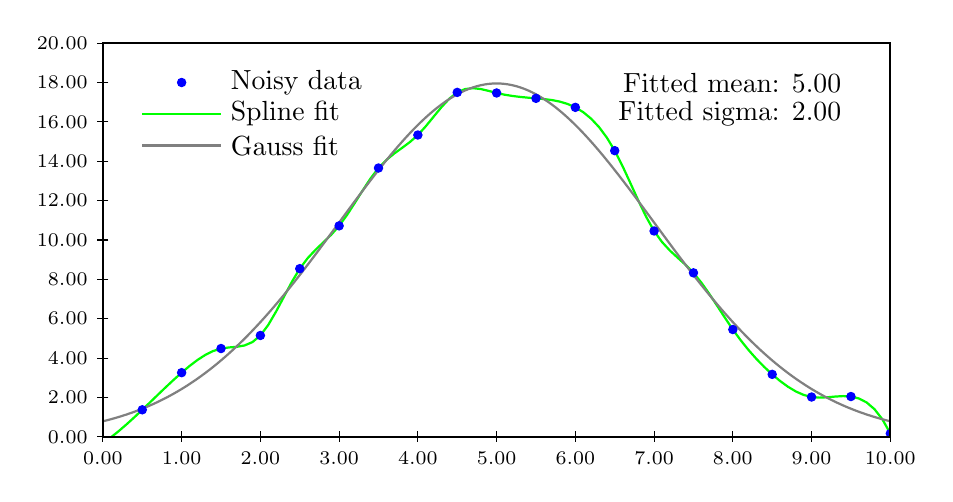
\begin{tikzpicture}
\begin{scope}[]
\pgfpathmoveto{ \pgfpointxy {0.0} {0.0}}
\pgfpathlineto{ \pgfpointxy {10.0} {0.0}}
\pgfpathlineto{ \pgfpointxy {10.0} {5.0}}
\pgfpathlineto{ \pgfpointxy {0.0} {5.0}}
\pgfpathclose
\pgfusepath{  clip, }
\begin{scope}[shift={(0.0,0.0)}]
\pgfsetxvec{\pgfpoint{1.0cm}{0cm}}
\pgfsetyvec{\pgfpoint{0cm}{0.25cm}}
\begin{scope}[shift={(0.0,0.0)}]
\begin{scope}[green,thick]
\pgfpathmoveto{ \pgfpointxy {0.0} {-0.3220822684578466}}
\pgfpathlineto{ \pgfpointxy {0.1} {-0.03179540914739956}}
\pgfpathlineto{ \pgfpointxy {0.2} {0.2885428151650948}}
\pgfpathlineto{ \pgfpointxy {0.3} {0.633328152486329}}
\pgfpathlineto{ \pgfpointxy {0.4} {0.9969563508229966}}
\pgfpathlineto{ \pgfpointxy {0.5} {1.3738231581817897}}
\pgfpathlineto{ \pgfpointxy {0.6} {1.7583243225694014}}
\pgfpathlineto{ \pgfpointxy {0.7} {2.144855591992525}}
\pgfpathlineto{ \pgfpointxy {0.8} {2.5278127144578533}}
\pgfpathlineto{ \pgfpointxy {0.9} {2.9015914379720784}}
\pgfpathlineto{ \pgfpointxy {1.0} {3.2605875105418933}}
\pgfpathlineto{ \pgfpointxy {1.1} {3.59798429165626}}
\pgfpathlineto{ \pgfpointxy {1.2} {3.9021155867332062}}
\pgfpathlineto{ \pgfpointxy {1.3} {4.160102812673034}}
\pgfpathlineto{ \pgfpointxy {1.4} {4.359067386376038}}
\pgfpathlineto{ \pgfpointxy {1.5} {4.486130724742518}}
\pgfpathlineto{ \pgfpointxy {1.6} {4.540874002276166}}
\pgfpathlineto{ \pgfpointxy {1.7} {4.572717423894254}}
\pgfpathlineto{ \pgfpointxy {1.8} {4.6435409521174424}}
\pgfpathlineto{ \pgfpointxy {1.9} {4.815224549466396}}
\pgfpathlineto{ \pgfpointxy {2.0} {5.149648178461778}}
\pgfpathlineto{ \pgfpointxy {2.1} {5.685601299272113}}
\pgfpathlineto{ \pgfpointxy {2.2} {6.3695113626573665}}
\pgfpathlineto{ \pgfpointxy {2.3} {7.124715317025358}}
\pgfpathlineto{ \pgfpointxy {2.4} {7.874550110783923}}
\pgfpathlineto{ \pgfpointxy {2.5} {8.54235269234088}}
\pgfpathlineto{ \pgfpointxy {2.6} {9.073464969531473}}
\pgfpathlineto{ \pgfpointxy {2.7} {9.50124868790061}}
\pgfpathlineto{ \pgfpointxy {2.8} {9.88107055242061}}
\pgfpathlineto{ \pgfpointxy {2.9} {10.268297268063803}}
\pgfpathlineto{ \pgfpointxy {3.0} {10.718295539802511}}
\pgfpathlineto{ \pgfpointxy {3.1} {11.268900377785958}}
\pgfpathlineto{ \pgfpointxy {3.2} {11.887820012870971}}
\pgfpathlineto{ \pgfpointxy {3.3} {12.52523098109127}}
\pgfpathlineto{ \pgfpointxy {3.4} {13.131309818480585}}
\pgfpathlineto{ \pgfpointxy {3.5} {13.656233061072639}}
\pgfpathlineto{ \pgfpointxy {3.6} {14.066283096326574}}
\pgfpathlineto{ \pgfpointxy {3.7} {14.392165717403207}}
\pgfpathlineto{ \pgfpointxy {3.8} {14.680692568888766}}
\pgfpathlineto{ \pgfpointxy {3.9} {14.978675295369484}}
\pgfpathlineto{ \pgfpointxy {4.0} {15.3329255414316}}
\pgfpathlineto{ \pgfpointxy {4.1} {15.773545607044694}}
\pgfpathlineto{ \pgfpointxy {4.2} {16.263800413711795}}
\pgfpathlineto{ \pgfpointxy {4.3} {16.75024553831928}}
\pgfpathlineto{ \pgfpointxy {4.4} {17.179436557753533}}
\pgfpathlineto{ \pgfpointxy {4.5} {17.497929048900925}}
\pgfpathlineto{ \pgfpointxy {4.6} {17.667544878429773}}
\pgfpathlineto{ \pgfpointxy {4.7} {17.711171072136075}}
\pgfpathlineto{ \pgfpointxy {4.8} {17.666960945597783}}
\pgfpathlineto{ \pgfpointxy {4.9} {17.57306781439283}}
\pgfpathlineto{ \pgfpointxy {5.0} {17.46764499409915}}
\pgfpathlineto{ \pgfpointxy {5.1} {17.38158457781227}}
\pgfpathlineto{ \pgfpointxy {5.2} {17.31673376869809}}
\pgfpathlineto{ \pgfpointxy {5.3} {17.267678547440084}}
\pgfpathlineto{ \pgfpointxy {5.4} {17.22900489472175}}
\pgfpathlineto{ \pgfpointxy {5.5} {17.195298791226566}}
\pgfpathlineto{ \pgfpointxy {5.6} {17.15975016321322}}
\pgfpathlineto{ \pgfpointxy {5.7} {17.109964719241223}}
\pgfpathlineto{ \pgfpointxy {5.8} {17.0321521134453}}
\pgfpathlineto{ \pgfpointxy {5.9} {16.912521999960166}}
\pgfpathlineto{ \pgfpointxy {6.0} {16.73728403292054}}
\pgfpathlineto{ \pgfpointxy {6.1} {16.492593096437812}}
\pgfpathlineto{ \pgfpointxy {6.2} {16.164384994530018}}
\pgfpathlineto{ \pgfpointxy {6.3} {15.738540761191885}}
\pgfpathlineto{ \pgfpointxy {6.4} {15.200941430418121}}
\pgfpathlineto{ \pgfpointxy {6.5} {14.537468036203448}}
\pgfpathlineto{ \pgfpointxy {6.6} {13.746955063475587}}
\pgfpathlineto{ \pgfpointxy {6.7} {12.880050800894296}}
\pgfpathlineto{ \pgfpointxy {6.8} {12.000356988052364}}
\pgfpathlineto{ \pgfpointxy {6.9} {11.171475364542555}}
\pgfpathlineto{ \pgfpointxy {7.0} {10.457007669957658}}
\pgfpathlineto{ \pgfpointxy {7.1} {9.900588706936261}}
\pgfpathlineto{ \pgfpointxy {7.2} {9.465985530300243}}
\pgfpathlineto{ \pgfpointxy {7.3} {9.096998257917303}}
\pgfpathlineto{ \pgfpointxy {7.4} {8.737427007655137}}
\pgfpathlineto{ \pgfpointxy {7.5} {8.331071897381452}}
\pgfpathlineto{ \pgfpointxy {7.6} {7.836306153830907}}
\pgfpathlineto{ \pgfpointxy {7.7} {7.269795439206012}}
\pgfpathlineto{ \pgfpointxy {7.8} {6.662778524576263}}
\pgfpathlineto{ \pgfpointxy {7.9} {6.046494181011129}}
\pgfpathlineto{ \pgfpointxy {8.0} {5.452181179580102}}
\pgfpathlineto{ \pgfpointxy {8.1} {4.905237179264141}}
\pgfpathlineto{ \pgfpointxy {8.2} {4.4076953906901215}}
\pgfpathlineto{ \pgfpointxy {8.3} {3.9557479123963915}}
\pgfpathlineto{ \pgfpointxy {8.4} {3.545586842921326}}
\pgfpathlineto{ \pgfpointxy {8.5} {3.173404280803272}}
\pgfpathlineto{ \pgfpointxy {8.6} {2.837587185462304}}
\pgfpathlineto{ \pgfpointxy {8.7} {2.545301959845368}}
\pgfpathlineto{ \pgfpointxy {8.8} {2.305909867781125}}
\pgfpathlineto{ \pgfpointxy {8.9} {2.128772173098246}}
\pgfpathlineto{ \pgfpointxy {9.0} {2.0232501396253917}}
\pgfpathlineto{ \pgfpointxy {9.1} {1.9919084111773382}}
\pgfpathlineto{ \pgfpointxy {9.2} {2.010125151513315}}
\pgfpathlineto{ \pgfpointxy {9.3} {2.046481904378665}}
\pgfpathlineto{ \pgfpointxy {9.4} {2.0695602135187294}}
\pgfpathlineto{ \pgfpointxy {9.5} {2.047941622678851}}
\pgfpathlineto{ \pgfpointxy {9.6} {1.9502076756043718}}
\pgfpathlineto{ \pgfpointxy {9.7} {1.744939916040635}}
\pgfpathlineto{ \pgfpointxy {9.8} {1.400719887732975}}
\pgfpathlineto{ \pgfpointxy {9.9} {0.8861291344267457}}
\pgfpathlineto{ \pgfpointxy {10.0} {0.16974919986728543}}
\pgfusepath{ stroke, }
\end{scope}
\begin{scope}[thick,gray]
\pgfpathmoveto{ \pgfpointxy {0.0} {0.7887735222102034}}
\pgfpathlineto{ \pgfpointxy {0.05} {0.8393826956517481}}
\pgfpathlineto{ \pgfpointxy {0.1} {0.892680947630374}}
\pgfpathlineto{ \pgfpointxy {0.15} {0.9487703099544526}}
\pgfpathlineto{ \pgfpointxy {0.2} {1.0077538632674794}}
\pgfpathlineto{ \pgfpointxy {0.25} {1.0697355373456514}}
\pgfpathlineto{ \pgfpointxy {0.3} {1.134819896183258}}
\pgfpathlineto{ \pgfpointxy {0.35} {1.203111907750662}}
\pgfpathlineto{ \pgfpointxy {0.4} {1.2747166983715252}}
\pgfpathlineto{ \pgfpointxy {0.45} {1.3497392917319906}}
\pgfpathlineto{ \pgfpointxy {0.5} {1.4282843326044656}}
\pgfpathlineto{ \pgfpointxy {0.55} {1.5104557954424003}}
\pgfpathlineto{ \pgfpointxy {0.6} {1.5963566780798044}}
\pgfpathlineto{ \pgfpointxy {0.65} {1.6860886808498898}}
\pgfpathlineto{ \pgfpointxy {0.7} {1.779751871521008}}
\pgfpathlineto{ \pgfpointxy {0.75} {1.8774443365345639}}
\pgfpathlineto{ \pgfpointxy {0.8} {1.9792618191185283}}
\pgfpathlineto{ \pgfpointxy {0.85} {2.0852973449411976}}
\pgfpathlineto{ \pgfpointxy {0.9} {2.1956408360624864}}
\pgfpathlineto{ \pgfpointxy {0.95} {2.310378714033865}}
\pgfpathlineto{ \pgfpointxy {1.0} {2.42959349309268}}
\pgfpathlineto{ \pgfpointxy {1.05} {2.5533633644912777}}
\pgfpathlineto{ \pgfpointxy {1.1} {2.6817617730958987}}
\pgfpathlineto{ \pgfpointxy {1.15} {2.8148569874838527}}
\pgfpathlineto{ \pgfpointxy {1.2} {2.95271166485958}}
\pgfpathlineto{ \pgfpointxy {1.25} {3.0953824122002476}}
\pgfpathlineto{ \pgfpointxy {1.3} {3.2429193451289016}}
\pgfpathlineto{ \pgfpointxy {1.35} {3.3953656460971313}}
\pgfpathlineto{ \pgfpointxy {1.4} {3.5527571235392896}}
\pgfpathlineto{ \pgfpointxy {1.45} {3.7151217737356554}}
\pgfpathlineto{ \pgfpointxy {1.5} {3.882479347192031}}
\pgfpathlineto{ \pgfpointxy {1.55} {4.0548409214074095}}
\pgfpathlineto{ \pgfpointxy {1.6} {4.232208481958889}}
\pgfpathlineto{ \pgfpointxy {1.65} {4.414574513883361}}
\pgfpathlineto{ \pgfpointxy {1.7} {4.601921605377953}}
\pgfpathlineto{ \pgfpointxy {1.75} {4.794222065875254}}
\pgfpathlineto{ \pgfpointxy {1.8} {4.991437560574411}}
\pgfpathlineto{ \pgfpointxy {1.85} {5.193518763524646}}
\pgfpathlineto{ \pgfpointxy {1.9} {5.400405031363236}}
\pgfpathlineto{ \pgfpointxy {1.95} {5.612024099804946}}
\pgfpathlineto{ \pgfpointxy {2.0} {5.828291804963986}}
\pgfpathlineto{ \pgfpointxy {2.05} {6.0491118315624055}}
\pgfpathlineto{ \pgfpointxy {2.1} {6.27437549004005}}
\pgfpathlineto{ \pgfpointxy {2.15} {6.503961524530807}}
\pgfpathlineto{ \pgfpointxy {2.2} {6.7377359536073405}}
\pgfpathlineto{ \pgfpointxy {2.25} {6.975551945622008}}
\pgfpathlineto{ \pgfpointxy {2.3} {7.217249730385189}}
\pgfpathlineto{ \pgfpointxy {2.35} {7.462656548823516}}
\pgfpathlineto{ \pgfpointxy {2.4} {7.71158664215013}}
\pgfpathlineto{ \pgfpointxy {2.45} {7.963841281956886}}
\pgfpathlineto{ \pgfpointxy {2.5} {8.219208842504782}}
\pgfpathlineto{ \pgfpointxy {2.55} {8.47746491634448}}
\pgfpathlineto{ \pgfpointxy {2.6} {8.73837247424338}}
\pgfpathlineto{ \pgfpointxy {2.65} {9.001682070230748}}
\pgfpathlineto{ \pgfpointxy {2.7} {9.267132092397667}}
\pgfpathlineto{ \pgfpointxy {2.75} {9.534449059905283}}
\pgfpathlineto{ \pgfpointxy {2.8} {9.803347966463585}}
\pgfpathlineto{ \pgfpointxy {2.85} {10.073532670344598}}
\pgfpathlineto{ \pgfpointxy {2.9} {10.344696330789311}}
\pgfpathlineto{ \pgfpointxy {2.95} {10.6165218904581}}
\pgfpathlineto{ \pgfpointxy {3.0} {10.888682603360296}}
\pgfpathlineto{ \pgfpointxy {3.05} {11.160842607482026}}
\pgfpathlineto{ \pgfpointxy {3.1} {11.432657541112373}}
\pgfpathlineto{ \pgfpointxy {3.15} {11.703775201648687}}
\pgfpathlineto{ \pgfpointxy {3.2} {11.973836245442861}}
\pgfpathlineto{ \pgfpointxy {3.25} {12.242474927033365}}
\pgfpathlineto{ \pgfpointxy {3.3} {12.509319875893764}}
\pgfpathlineto{ \pgfpointxy {3.35} {12.773994908618867}}
\pgfpathlineto{ \pgfpointxy {3.4} {13.036119874265678}}
\pgfpathlineto{ \pgfpointxy {3.45} {13.295311530369304}}
\pgfpathlineto{ \pgfpointxy {3.5} {13.551184446965188}}
\pgfpathlineto{ \pgfpointxy {3.55} {13.803351935769804}}
\pgfpathlineto{ \pgfpointxy {3.6} {14.051427001503281}}
\pgfpathlineto{ \pgfpointxy {3.65} {14.295023312180714}}
\pgfpathlineto{ \pgfpointxy {3.7} {14.533756185055205}}
\pgfpathlineto{ \pgfpointxy {3.75} {14.767243584765959}}
\pgfpathlineto{ \pgfpointxy {3.8} {14.995107130130082}}
\pgfpathlineto{ \pgfpointxy {3.85} {15.216973105918132}}
\pgfpathlineto{ \pgfpointxy {3.9} {15.432473475871411}}
\pgfpathlineto{ \pgfpointxy {3.95} {15.64124689315482}}
\pgfpathlineto{ \pgfpointxy {4.0} {15.84293970439265}}
\pgfpathlineto{ \pgfpointxy {4.05} {16.037206943407437}}
\pgfpathlineto{ \pgfpointxy {4.1} {16.223713310773366}}
\pgfpathlineto{ \pgfpointxy {4.15} {16.40213413530702}}
\pgfpathlineto{ \pgfpointxy {4.2} {16.572156313648794}}
\pgfpathlineto{ \pgfpointxy {4.25} {16.73347922413886}}
\pgfpathlineto{ \pgfpointxy {4.3} {16.885815611261478}}
\pgfpathlineto{ \pgfpointxy {4.35} {17.028892437021163}}
\pgfpathlineto{ \pgfpointxy {4.4} {17.162451695722886}}
\pgfpathlineto{ \pgfpointxy {4.45} {17.28625118875603}}
\pgfpathlineto{ \pgfpointxy {4.5} {17.40006525612754}}
\pgfpathlineto{ \pgfpointxy {4.55} {17.503685461653063}}
\pgfpathlineto{ \pgfpointxy {4.6} {17.596921228894864}}
\pgfpathlineto{ \pgfpointxy {4.65} {17.679600425131426}}
\pgfpathlineto{ \pgfpointxy {4.7} {17.751569890854366}}
\pgfpathlineto{ \pgfpointxy {4.75} {17.8126959125131}}
\pgfpathlineto{ \pgfpointxy {4.8} {17.862864636464906}}
\pgfpathlineto{ \pgfpointxy {4.85} {17.90198242233675}}
\pgfpathlineto{ \pgfpointxy {4.9} {17.929976134263764}}
\pgfpathlineto{ \pgfpointxy {4.95} {17.946793368736568}}
\pgfpathlineto{ \pgfpointxy {5.0} {17.952402618063857}}
\pgfpathlineto{ \pgfpointxy {5.05} {17.946793368736568}}
\pgfpathlineto{ \pgfpointxy {5.1} {17.929976134263764}}
\pgfpathlineto{ \pgfpointxy {5.15} {17.90198242233675}}
\pgfpathlineto{ \pgfpointxy {5.2} {17.862864636464906}}
\pgfpathlineto{ \pgfpointxy {5.25} {17.8126959125131}}
\pgfpathlineto{ \pgfpointxy {5.3} {17.751569890854366}}
\pgfpathlineto{ \pgfpointxy {5.35} {17.679600425131426}}
\pgfpathlineto{ \pgfpointxy {5.4} {17.596921228894864}}
\pgfpathlineto{ \pgfpointxy {5.45} {17.503685461653063}}
\pgfpathlineto{ \pgfpointxy {5.5} {17.40006525612754}}
\pgfpathlineto{ \pgfpointxy {5.55} {17.28625118875603}}
\pgfpathlineto{ \pgfpointxy {5.6} {17.162451695722886}}
\pgfpathlineto{ \pgfpointxy {5.65} {17.028892437021163}}
\pgfpathlineto{ \pgfpointxy {5.7} {16.885815611261478}}
\pgfpathlineto{ \pgfpointxy {5.75} {16.73347922413886}}
\pgfpathlineto{ \pgfpointxy {5.8} {16.572156313648794}}
\pgfpathlineto{ \pgfpointxy {5.85} {16.40213413530702}}
\pgfpathlineto{ \pgfpointxy {5.9} {16.223713310773366}}
\pgfpathlineto{ \pgfpointxy {5.95} {16.037206943407437}}
\pgfpathlineto{ \pgfpointxy {6.0} {15.84293970439265}}
\pgfpathlineto{ \pgfpointxy {6.05} {15.64124689315482}}
\pgfpathlineto{ \pgfpointxy {6.1} {15.432473475871413}}
\pgfpathlineto{ \pgfpointxy {6.15} {15.21697310591813}}
\pgfpathlineto{ \pgfpointxy {6.2} {14.995107130130082}}
\pgfpathlineto{ \pgfpointxy {6.25} {14.767243584765959}}
\pgfpathlineto{ \pgfpointxy {6.3} {14.533756185055205}}
\pgfpathlineto{ \pgfpointxy {6.35} {14.295023312180716}}
\pgfpathlineto{ \pgfpointxy {6.4} {14.05142700150328}}
\pgfpathlineto{ \pgfpointxy {6.45} {13.803351935769804}}
\pgfpathlineto{ \pgfpointxy {6.5} {13.551184446965188}}
\pgfpathlineto{ \pgfpointxy {6.55} {13.295311530369304}}
\pgfpathlineto{ \pgfpointxy {6.6} {13.03611987426568}}
\pgfpathlineto{ \pgfpointxy {6.65} {12.773994908618866}}
\pgfpathlineto{ \pgfpointxy {6.7} {12.509319875893764}}
\pgfpathlineto{ \pgfpointxy {6.75} {12.242474927033365}}
\pgfpathlineto{ \pgfpointxy {6.8} {11.973836245442861}}
\pgfpathlineto{ \pgfpointxy {6.85} {11.70377520164869}}
\pgfpathlineto{ \pgfpointxy {6.9} {11.43265754111237}}
\pgfpathlineto{ \pgfpointxy {6.95} {11.160842607482026}}
\pgfpathlineto{ \pgfpointxy {7.0} {10.888682603360296}}
\pgfpathlineto{ \pgfpointxy {7.05} {10.6165218904581}}
\pgfpathlineto{ \pgfpointxy {7.1} {10.344696330789315}}
\pgfpathlineto{ \pgfpointxy {7.15} {10.073532670344594}}
\pgfpathlineto{ \pgfpointxy {7.2} {9.803347966463585}}
\pgfpathlineto{ \pgfpointxy {7.25} {9.534449059905283}}
\pgfpathlineto{ \pgfpointxy {7.3} {9.267132092397667}}
\pgfpathlineto{ \pgfpointxy {7.35} {9.00168207023075}}
\pgfpathlineto{ \pgfpointxy {7.4} {8.738372474243379}}
\pgfpathlineto{ \pgfpointxy {7.45} {8.47746491634448}}
\pgfpathlineto{ \pgfpointxy {7.5} {8.219208842504782}}
\pgfpathlineto{ \pgfpointxy {7.55} {7.963841281956886}}
\pgfpathlineto{ \pgfpointxy {7.6} {7.711586642150132}}
\pgfpathlineto{ \pgfpointxy {7.65} {7.462656548823513}}
\pgfpathlineto{ \pgfpointxy {7.7} {7.217249730385189}}
\pgfpathlineto{ \pgfpointxy {7.75} {6.975551945622008}}
\pgfpathlineto{ \pgfpointxy {7.8} {6.7377359536073405}}
\pgfpathlineto{ \pgfpointxy {7.85} {6.503961524530809}}
\pgfpathlineto{ \pgfpointxy {7.9} {6.274375490040049}}
\pgfpathlineto{ \pgfpointxy {7.95} {6.0491118315624055}}
\pgfpathlineto{ \pgfpointxy {8.0} {5.828291804963986}}
\pgfpathlineto{ \pgfpointxy {8.05} {5.612024099804942}}
\pgfpathlineto{ \pgfpointxy {8.1} {5.4004050313632375}}
\pgfpathlineto{ \pgfpointxy {8.15} {5.193518763524644}}
\pgfpathlineto{ \pgfpointxy {8.2} {4.991437560574414}}
\pgfpathlineto{ \pgfpointxy {8.25} {4.794222065875254}}
\pgfpathlineto{ \pgfpointxy {8.3} {4.60192160537795}}
\pgfpathlineto{ \pgfpointxy {8.35} {4.4145745138833625}}
\pgfpathlineto{ \pgfpointxy {8.4} {4.232208481958887}}
\pgfpathlineto{ \pgfpointxy {8.45} {4.054840921407412}}
\pgfpathlineto{ \pgfpointxy {8.5} {3.882479347192031}}
\pgfpathlineto{ \pgfpointxy {8.55} {3.7151217737356528}}
\pgfpathlineto{ \pgfpointxy {8.6} {3.55275712353929}}
\pgfpathlineto{ \pgfpointxy {8.65} {3.3953656460971304}}
\pgfpathlineto{ \pgfpointxy {8.7} {3.2429193451289042}}
\pgfpathlineto{ \pgfpointxy {8.75} {3.0953824122002476}}
\pgfpathlineto{ \pgfpointxy {8.8} {2.9527116648595775}}
\pgfpathlineto{ \pgfpointxy {8.85} {2.8148569874838545}}
\pgfpathlineto{ \pgfpointxy {8.9} {2.681761773095898}}
\pgfpathlineto{ \pgfpointxy {8.95} {2.55336336449128}}
\pgfpathlineto{ \pgfpointxy {9.0} {2.42959349309268}}
\pgfpathlineto{ \pgfpointxy {9.05} {2.310378714033863}}
\pgfpathlineto{ \pgfpointxy {9.1} {2.1956408360624864}}
\pgfpathlineto{ \pgfpointxy {9.15} {2.0852973449411976}}
\pgfpathlineto{ \pgfpointxy {9.2} {1.97926181911853}}
\pgfpathlineto{ \pgfpointxy {9.25} {1.8774443365345639}}
\pgfpathlineto{ \pgfpointxy {9.3} {1.7797518715210063}}
\pgfpathlineto{ \pgfpointxy {9.35} {1.6860886808498898}}
\pgfpathlineto{ \pgfpointxy {9.4} {1.5963566780798044}}
\pgfpathlineto{ \pgfpointxy {9.45} {1.5104557954424018}}
\pgfpathlineto{ \pgfpointxy {9.5} {1.4282843326044656}}
\pgfpathlineto{ \pgfpointxy {9.55} {1.3497392917319893}}
\pgfpathlineto{ \pgfpointxy {9.6} {1.2747166983715252}}
\pgfpathlineto{ \pgfpointxy {9.65} {1.203111907750662}}
\pgfpathlineto{ \pgfpointxy {9.7} {1.1348198961832596}}
\pgfpathlineto{ \pgfpointxy {9.75} {1.0697355373456514}}
\pgfpathlineto{ \pgfpointxy {9.8} {1.0077538632674785}}
\pgfpathlineto{ \pgfpointxy {9.85} {0.9487703099544526}}
\pgfpathlineto{ \pgfpointxy {9.9} {0.892680947630374}}
\pgfpathlineto{ \pgfpointxy {9.95} {0.8393826956517488}}
\pgfpathlineto{ \pgfpointxy {10.0} {0.7887735222102034}}
\pgfusepath{ stroke, }
\end{scope}
\node at (0.0,-0.3220822684578466) [circle,inner sep=0.0pt,minimum width =3.0pt,minimum height=3.0pt,draw=blue,fill=blue] {}; 
\node at (0.5,1.3738231581817897) [circle,inner sep=0.0pt,minimum width =3.0pt,minimum height=3.0pt,draw=blue,fill=blue] {}; 
\node at (1.0,3.2605875105418933) [circle,inner sep=0.0pt,minimum width =3.0pt,minimum height=3.0pt,draw=blue,fill=blue] {}; 
\node at (1.5,4.486130724742518) [circle,inner sep=0.0pt,minimum width =3.0pt,minimum height=3.0pt,draw=blue,fill=blue] {}; 
\node at (2.0,5.149648178461778) [circle,inner sep=0.0pt,minimum width =3.0pt,minimum height=3.0pt,draw=blue,fill=blue] {}; 
\node at (2.5,8.54235269234088) [circle,inner sep=0.0pt,minimum width =3.0pt,minimum height=3.0pt,draw=blue,fill=blue] {}; 
\node at (3.0,10.718295539802511) [circle,inner sep=0.0pt,minimum width =3.0pt,minimum height=3.0pt,draw=blue,fill=blue] {}; 
\node at (3.5,13.656233061072639) [circle,inner sep=0.0pt,minimum width =3.0pt,minimum height=3.0pt,draw=blue,fill=blue] {}; 
\node at (4.0,15.3329255414316) [circle,inner sep=0.0pt,minimum width =3.0pt,minimum height=3.0pt,draw=blue,fill=blue] {}; 
\node at (4.5,17.497929048900925) [circle,inner sep=0.0pt,minimum width =3.0pt,minimum height=3.0pt,draw=blue,fill=blue] {}; 
\node at (5.0,17.467644994099146) [circle,inner sep=0.0pt,minimum width =3.0pt,minimum height=3.0pt,draw=blue,fill=blue] {}; 
\node at (5.5,17.195298791226566) [circle,inner sep=0.0pt,minimum width =3.0pt,minimum height=3.0pt,draw=blue,fill=blue] {}; 
\node at (6.0,16.73728403292054) [circle,inner sep=0.0pt,minimum width =3.0pt,minimum height=3.0pt,draw=blue,fill=blue] {}; 
\node at (6.5,14.537468036203448) [circle,inner sep=0.0pt,minimum width =3.0pt,minimum height=3.0pt,draw=blue,fill=blue] {}; 
\node at (7.0,10.457007669957658) [circle,inner sep=0.0pt,minimum width =3.0pt,minimum height=3.0pt,draw=blue,fill=blue] {}; 
\node at (7.5,8.331071897381452) [circle,inner sep=0.0pt,minimum width =3.0pt,minimum height=3.0pt,draw=blue,fill=blue] {}; 
\node at (8.0,5.452181179580102) [circle,inner sep=0.0pt,minimum width =3.0pt,minimum height=3.0pt,draw=blue,fill=blue] {}; 
\node at (8.5,3.173404280803272) [circle,inner sep=0.0pt,minimum width =3.0pt,minimum height=3.0pt,draw=blue,fill=blue] {}; 
\node at (9.0,2.0232501396253917) [circle,inner sep=0.0pt,minimum width =3.0pt,minimum height=3.0pt,draw=blue,fill=blue] {}; 
\node at (9.5,2.047941622678851) [circle,inner sep=0.0pt,minimum width =3.0pt,minimum height=3.0pt,draw=blue,fill=blue] {}; 
\node at (10.0,0.16974919986728554) [circle,inner sep=0.0pt,minimum width =3.0pt,minimum height=3.0pt,draw=blue,fill=blue] {}; 
\end{scope}
\pgfsetxvec{\pgfpoint{1cm}{0cm}}
\pgfsetyvec{\pgfpoint{0cm}{1cm}}
\end{scope}
\end{scope}
\begin{scope}[shift={(0.0,0.0)}]
\pgfsetxvec{\pgfpoint{1.0cm}{0cm}}
\pgfsetyvec{\pgfpoint{0cm}{0.25cm}}
\begin{scope}[shift={(0.0,0.0)}]
\begin{scope}[yshift=0cm]
\draw[black] [shift={(0.0,0.0)}] (0,2pt) -- (0,-2pt) node[below]{ \scriptsize{\num[round-mode=places,round-precision=2]{0}}};
\draw[black] [shift={(1.0,0.0)}] (0,2pt) -- (0,-2pt) node[below]{ \scriptsize{\num[round-mode=places,round-precision=2]{1}}};
\draw[black] [shift={(2.0,0.0)}] (0,2pt) -- (0,-2pt) node[below]{ \scriptsize{\num[round-mode=places,round-precision=2]{2}}};
\draw[black] [shift={(3.0,0.0)}] (0,2pt) -- (0,-2pt) node[below]{ \scriptsize{\num[round-mode=places,round-precision=2]{3}}};
\draw[black] [shift={(4.0,0.0)}] (0,2pt) -- (0,-2pt) node[below]{ \scriptsize{\num[round-mode=places,round-precision=2]{4}}};
\draw[black] [shift={(5.0,0.0)}] (0,2pt) -- (0,-2pt) node[below]{ \scriptsize{\num[round-mode=places,round-precision=2]{5}}};
\draw[black] [shift={(6.0,0.0)}] (0,2pt) -- (0,-2pt) node[below]{ \scriptsize{\num[round-mode=places,round-precision=2]{6}}};
\draw[black] [shift={(7.0,0.0)}] (0,2pt) -- (0,-2pt) node[below]{ \scriptsize{\num[round-mode=places,round-precision=2]{7}}};
\draw[black] [shift={(8.0,0.0)}] (0,2pt) -- (0,-2pt) node[below]{ \scriptsize{\num[round-mode=places,round-precision=2]{8}}};
\draw[black] [shift={(9.0,0.0)}] (0,2pt) -- (0,-2pt) node[below]{ \scriptsize{\num[round-mode=places,round-precision=2]{9}}};
\draw[black] [shift={(10.0,0.0)}] (0,2pt) -- (0,-2pt) node[below]{ \scriptsize{\num[round-mode=places,round-precision=2]{10}}};
\end{scope}
\begin{scope}[xshift=0cm]
\draw[black] [shift={(0.0,0.0)}] (2pt,0) -- (-2pt,0) node[left]{ \scriptsize{\num[round-mode=places,round-precision=2]{0}}};
\draw[black] [shift={(0.0,2.0)}] (2pt,0) -- (-2pt,0) node[left]{ \scriptsize{\num[round-mode=places,round-precision=2]{2}}};
\draw[black] [shift={(0.0,4.0)}] (2pt,0) -- (-2pt,0) node[left]{ \scriptsize{\num[round-mode=places,round-precision=2]{4}}};
\draw[black] [shift={(0.0,6.0)}] (2pt,0) -- (-2pt,0) node[left]{ \scriptsize{\num[round-mode=places,round-precision=2]{6}}};
\draw[black] [shift={(0.0,8.0)}] (2pt,0) -- (-2pt,0) node[left]{ \scriptsize{\num[round-mode=places,round-precision=2]{8}}};
\draw[black] [shift={(0.0,10.0)}] (2pt,0) -- (-2pt,0) node[left]{ \scriptsize{\num[round-mode=places,round-precision=2]{10}}};
\draw[black] [shift={(0.0,12.0)}] (2pt,0) -- (-2pt,0) node[left]{ \scriptsize{\num[round-mode=places,round-precision=2]{12}}};
\draw[black] [shift={(0.0,14.0)}] (2pt,0) -- (-2pt,0) node[left]{ \scriptsize{\num[round-mode=places,round-precision=2]{14}}};
\draw[black] [shift={(0.0,16.0)}] (2pt,0) -- (-2pt,0) node[left]{ \scriptsize{\num[round-mode=places,round-precision=2]{16}}};
\draw[black] [shift={(0.0,18.0)}] (2pt,0) -- (-2pt,0) node[left]{ \scriptsize{\num[round-mode=places,round-precision=2]{18}}};
\draw[black] [shift={(0.0,20.0)}] (2pt,0) -- (-2pt,0) node[left]{ \scriptsize{\num[round-mode=places,round-precision=2]{20}}};
\end{scope}
\begin{scope}[thick,black,fill=white]
\pgfpathmoveto{ \pgfpointxy {0.0} {0.0}}
\pgfpathlineto{ \pgfpointxy {10.0} {0.0}}
\pgfpathlineto{ \pgfpointxy {10.0} {20.0}}
\pgfpathlineto{ \pgfpointxy {0.0} {20.0}}
\pgfpathclose
\pgfusepath{ stroke, }
\end{scope}
\end{scope}
\pgfsetxvec{\pgfpoint{1cm}{0cm}}
\pgfsetyvec{\pgfpoint{0cm}{1cm}}
\end{scope}
\node at (1.0,4.5) [circle,inner sep=0.0pt,minimum width =3.0pt,minimum height=3.0pt,draw=blue,fill=blue] {}; 
\node[right,] at (1.5,4.5) {Noisy data};
\draw[draw=green,thick] (0.5,4.1) -- (1.5,4.1);
\node[right,] at (1.5,4.1) {Spline fit};
\draw[thick,gray] (0.5,3.7) -- (1.5,3.7);
\node[right,] at (1.5,3.7) {Gauss fit};
\node[left] at (9.5,4.5) {Fitted mean:  5.00};
\node[left] at (9.5,4.1) {Fitted sigma:  2.00};
\end{tikzpicture}
\end{document}

\captionsetup{singlelinecheck=off}
\caption[asdf]{Some Gauss smeared data points, fitted with the Gaussian function. Fit parameters are printed in the plot. 
A spline fit is also plotted.}
\end{figure}
\begin{figure}[H]
\centering
\documentclass{standalone}
\ifx\HCode\UnDef\else\def\pgfsysdriver{pgfsys-tex4ht.def}\fi
\usepackage{tikz}
\usepackage{color}
\usepackage{siunitx}
\usetikzlibrary{arrows,shapes}
\begin{document}
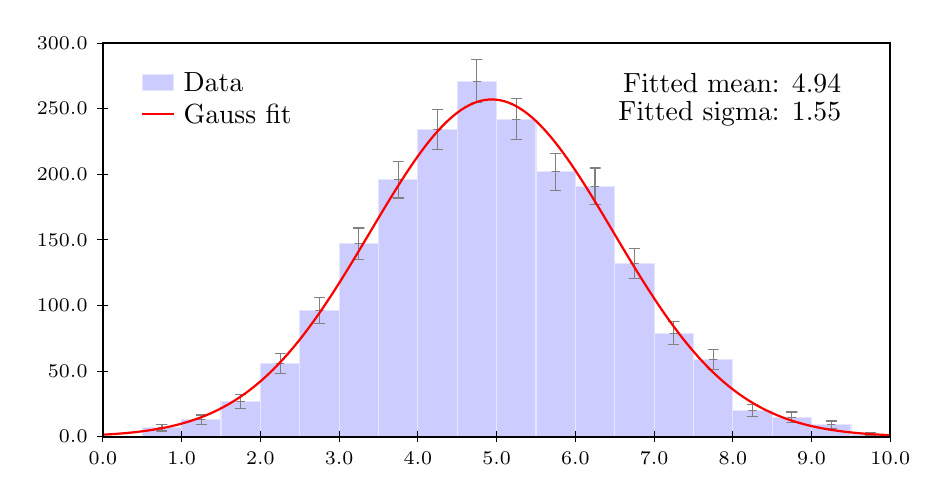
\begin{tikzpicture}
\node[left] at (9.5,4.5) {Fitted mean:  4.94};
\node[left] at (9.5,4.1) {Fitted sigma:  1.55};
\begin{scope}[]
\pgfpathmoveto{ \pgfpointxy {0.0} {0.0}}
\pgfpathlineto{ \pgfpointxy {10.0} {0.0}}
\pgfpathlineto{ \pgfpointxy {10.0} {5.0}}
\pgfpathlineto{ \pgfpointxy {0.0} {5.0}}
\pgfpathclose
\pgfusepath{  clip, }
\begin{scope}[shift={(0.0,0.0)}]
\pgfsetxvec{\pgfpoint{1.0cm}{0cm}}
\pgfsetyvec{\pgfpoint{0cm}{0.016666668cm}}
\begin{scope}[shift={(0.0,0.0)}]
\begin{scope}[draw=blue!10,fill=blue!20]
\pgfpathmoveto{ \pgfpointxy {10.0} {0.0}}
\pgfpathlineto{ \pgfpointxy {10.0} {2.0}}
\pgfpathlineto{ \pgfpointxy {9.5} {2.0}}
\pgfpathlineto{ \pgfpointxy {9.5} {9.0}}
\pgfpathlineto{ \pgfpointxy {9.0} {9.0}}
\pgfpathlineto{ \pgfpointxy {9.0} {15.0}}
\pgfpathlineto{ \pgfpointxy {8.5} {15.0}}
\pgfpathlineto{ \pgfpointxy {8.5} {20.0}}
\pgfpathlineto{ \pgfpointxy {8.0} {20.0}}
\pgfpathlineto{ \pgfpointxy {8.0} {59.0}}
\pgfpathlineto{ \pgfpointxy {7.5} {59.0}}
\pgfpathlineto{ \pgfpointxy {7.5} {79.0}}
\pgfpathlineto{ \pgfpointxy {7.0} {79.0}}
\pgfpathlineto{ \pgfpointxy {7.0} {132.0}}
\pgfpathlineto{ \pgfpointxy {6.5} {132.0}}
\pgfpathlineto{ \pgfpointxy {6.5} {191.0}}
\pgfpathlineto{ \pgfpointxy {6.0} {191.0}}
\pgfpathlineto{ \pgfpointxy {6.0} {202.0}}
\pgfpathlineto{ \pgfpointxy {5.5} {202.0}}
\pgfpathlineto{ \pgfpointxy {5.5} {242.0}}
\pgfpathlineto{ \pgfpointxy {5.0} {242.0}}
\pgfpathlineto{ \pgfpointxy {5.0} {271.0}}
\pgfpathlineto{ \pgfpointxy {4.5} {271.0}}
\pgfpathlineto{ \pgfpointxy {4.5} {234.0}}
\pgfpathlineto{ \pgfpointxy {4.0} {234.0}}
\pgfpathlineto{ \pgfpointxy {4.0} {196.0}}
\pgfpathlineto{ \pgfpointxy {3.5} {196.0}}
\pgfpathlineto{ \pgfpointxy {3.5} {147.0}}
\pgfpathlineto{ \pgfpointxy {3.0} {147.0}}
\pgfpathlineto{ \pgfpointxy {3.0} {96.0}}
\pgfpathlineto{ \pgfpointxy {2.5} {96.0}}
\pgfpathlineto{ \pgfpointxy {2.5} {56.0}}
\pgfpathlineto{ \pgfpointxy {2.0} {56.0}}
\pgfpathlineto{ \pgfpointxy {2.0} {27.0}}
\pgfpathlineto{ \pgfpointxy {1.5} {27.0}}
\pgfpathlineto{ \pgfpointxy {1.5} {13.0}}
\pgfpathlineto{ \pgfpointxy {1.0} {13.0}}
\pgfpathlineto{ \pgfpointxy {1.0} {7.0}}
\pgfpathlineto{ \pgfpointxy {0.5} {7.0}}
\pgfpathlineto{ \pgfpointxy {0.5} {0.0}}
\pgfpathlineto{ \pgfpointxy {0.0} {0.0}}
\pgfpathlineto{ \pgfpointxy {0.0} {0.0}}
\pgfusepath{ stroke, fill, }
\end{scope}
\begin{scope}[draw=blue!10,fill=blue!20]
\pgfpathmoveto{ \pgfpointxy {10.0} {0.0}}
\pgfpathlineto{ \pgfpointxy {10.0} {0.0}}
\pgfusepath{ stroke, }
\end{scope}
\begin{scope}[draw=blue!10,fill=blue!20]
\pgfpathmoveto{ \pgfpointxy {10.0} {2.0}}
\pgfpathlineto{ \pgfpointxy {10.0} {0.0}}
\pgfusepath{ stroke, }
\end{scope}
\begin{scope}[draw=blue!10,fill=blue!20]
\pgfpathmoveto{ \pgfpointxy {9.5} {2.0}}
\pgfpathlineto{ \pgfpointxy {9.5} {0.0}}
\pgfusepath{ stroke, }
\end{scope}
\begin{scope}[draw=blue!10,fill=blue!20]
\pgfpathmoveto{ \pgfpointxy {9.5} {9.0}}
\pgfpathlineto{ \pgfpointxy {9.5} {0.0}}
\pgfusepath{ stroke, }
\end{scope}
\begin{scope}[draw=blue!10,fill=blue!20]
\pgfpathmoveto{ \pgfpointxy {9.0} {9.0}}
\pgfpathlineto{ \pgfpointxy {9.0} {0.0}}
\pgfusepath{ stroke, }
\end{scope}
\begin{scope}[draw=blue!10,fill=blue!20]
\pgfpathmoveto{ \pgfpointxy {9.0} {15.0}}
\pgfpathlineto{ \pgfpointxy {9.0} {0.0}}
\pgfusepath{ stroke, }
\end{scope}
\begin{scope}[draw=blue!10,fill=blue!20]
\pgfpathmoveto{ \pgfpointxy {8.5} {15.0}}
\pgfpathlineto{ \pgfpointxy {8.5} {0.0}}
\pgfusepath{ stroke, }
\end{scope}
\begin{scope}[draw=blue!10,fill=blue!20]
\pgfpathmoveto{ \pgfpointxy {8.5} {20.0}}
\pgfpathlineto{ \pgfpointxy {8.5} {0.0}}
\pgfusepath{ stroke, }
\end{scope}
\begin{scope}[draw=blue!10,fill=blue!20]
\pgfpathmoveto{ \pgfpointxy {8.0} {20.0}}
\pgfpathlineto{ \pgfpointxy {8.0} {0.0}}
\pgfusepath{ stroke, }
\end{scope}
\begin{scope}[draw=blue!10,fill=blue!20]
\pgfpathmoveto{ \pgfpointxy {8.0} {59.0}}
\pgfpathlineto{ \pgfpointxy {8.0} {0.0}}
\pgfusepath{ stroke, }
\end{scope}
\begin{scope}[draw=blue!10,fill=blue!20]
\pgfpathmoveto{ \pgfpointxy {7.5} {59.0}}
\pgfpathlineto{ \pgfpointxy {7.5} {0.0}}
\pgfusepath{ stroke, }
\end{scope}
\begin{scope}[draw=blue!10,fill=blue!20]
\pgfpathmoveto{ \pgfpointxy {7.5} {79.0}}
\pgfpathlineto{ \pgfpointxy {7.5} {0.0}}
\pgfusepath{ stroke, }
\end{scope}
\begin{scope}[draw=blue!10,fill=blue!20]
\pgfpathmoveto{ \pgfpointxy {7.0} {79.0}}
\pgfpathlineto{ \pgfpointxy {7.0} {0.0}}
\pgfusepath{ stroke, }
\end{scope}
\begin{scope}[draw=blue!10,fill=blue!20]
\pgfpathmoveto{ \pgfpointxy {7.0} {132.0}}
\pgfpathlineto{ \pgfpointxy {7.0} {0.0}}
\pgfusepath{ stroke, }
\end{scope}
\begin{scope}[draw=blue!10,fill=blue!20]
\pgfpathmoveto{ \pgfpointxy {6.5} {132.0}}
\pgfpathlineto{ \pgfpointxy {6.5} {0.0}}
\pgfusepath{ stroke, }
\end{scope}
\begin{scope}[draw=blue!10,fill=blue!20]
\pgfpathmoveto{ \pgfpointxy {6.5} {191.0}}
\pgfpathlineto{ \pgfpointxy {6.5} {0.0}}
\pgfusepath{ stroke, }
\end{scope}
\begin{scope}[draw=blue!10,fill=blue!20]
\pgfpathmoveto{ \pgfpointxy {6.0} {191.0}}
\pgfpathlineto{ \pgfpointxy {6.0} {0.0}}
\pgfusepath{ stroke, }
\end{scope}
\begin{scope}[draw=blue!10,fill=blue!20]
\pgfpathmoveto{ \pgfpointxy {6.0} {202.0}}
\pgfpathlineto{ \pgfpointxy {6.0} {0.0}}
\pgfusepath{ stroke, }
\end{scope}
\begin{scope}[draw=blue!10,fill=blue!20]
\pgfpathmoveto{ \pgfpointxy {5.5} {202.0}}
\pgfpathlineto{ \pgfpointxy {5.5} {0.0}}
\pgfusepath{ stroke, }
\end{scope}
\begin{scope}[draw=blue!10,fill=blue!20]
\pgfpathmoveto{ \pgfpointxy {5.5} {242.0}}
\pgfpathlineto{ \pgfpointxy {5.5} {0.0}}
\pgfusepath{ stroke, }
\end{scope}
\begin{scope}[draw=blue!10,fill=blue!20]
\pgfpathmoveto{ \pgfpointxy {5.0} {242.0}}
\pgfpathlineto{ \pgfpointxy {5.0} {0.0}}
\pgfusepath{ stroke, }
\end{scope}
\begin{scope}[draw=blue!10,fill=blue!20]
\pgfpathmoveto{ \pgfpointxy {5.0} {271.0}}
\pgfpathlineto{ \pgfpointxy {5.0} {0.0}}
\pgfusepath{ stroke, }
\end{scope}
\begin{scope}[draw=blue!10,fill=blue!20]
\pgfpathmoveto{ \pgfpointxy {4.5} {271.0}}
\pgfpathlineto{ \pgfpointxy {4.5} {0.0}}
\pgfusepath{ stroke, }
\end{scope}
\begin{scope}[draw=blue!10,fill=blue!20]
\pgfpathmoveto{ \pgfpointxy {4.5} {234.0}}
\pgfpathlineto{ \pgfpointxy {4.5} {0.0}}
\pgfusepath{ stroke, }
\end{scope}
\begin{scope}[draw=blue!10,fill=blue!20]
\pgfpathmoveto{ \pgfpointxy {4.0} {234.0}}
\pgfpathlineto{ \pgfpointxy {4.0} {0.0}}
\pgfusepath{ stroke, }
\end{scope}
\begin{scope}[draw=blue!10,fill=blue!20]
\pgfpathmoveto{ \pgfpointxy {4.0} {196.0}}
\pgfpathlineto{ \pgfpointxy {4.0} {0.0}}
\pgfusepath{ stroke, }
\end{scope}
\begin{scope}[draw=blue!10,fill=blue!20]
\pgfpathmoveto{ \pgfpointxy {3.5} {196.0}}
\pgfpathlineto{ \pgfpointxy {3.5} {0.0}}
\pgfusepath{ stroke, }
\end{scope}
\begin{scope}[draw=blue!10,fill=blue!20]
\pgfpathmoveto{ \pgfpointxy {3.5} {147.0}}
\pgfpathlineto{ \pgfpointxy {3.5} {0.0}}
\pgfusepath{ stroke, }
\end{scope}
\begin{scope}[draw=blue!10,fill=blue!20]
\pgfpathmoveto{ \pgfpointxy {3.0} {147.0}}
\pgfpathlineto{ \pgfpointxy {3.0} {0.0}}
\pgfusepath{ stroke, }
\end{scope}
\begin{scope}[draw=blue!10,fill=blue!20]
\pgfpathmoveto{ \pgfpointxy {3.0} {96.0}}
\pgfpathlineto{ \pgfpointxy {3.0} {0.0}}
\pgfusepath{ stroke, }
\end{scope}
\begin{scope}[draw=blue!10,fill=blue!20]
\pgfpathmoveto{ \pgfpointxy {2.5} {96.0}}
\pgfpathlineto{ \pgfpointxy {2.5} {0.0}}
\pgfusepath{ stroke, }
\end{scope}
\begin{scope}[draw=blue!10,fill=blue!20]
\pgfpathmoveto{ \pgfpointxy {2.5} {56.0}}
\pgfpathlineto{ \pgfpointxy {2.5} {0.0}}
\pgfusepath{ stroke, }
\end{scope}
\begin{scope}[draw=blue!10,fill=blue!20]
\pgfpathmoveto{ \pgfpointxy {2.0} {56.0}}
\pgfpathlineto{ \pgfpointxy {2.0} {0.0}}
\pgfusepath{ stroke, }
\end{scope}
\begin{scope}[draw=blue!10,fill=blue!20]
\pgfpathmoveto{ \pgfpointxy {2.0} {27.0}}
\pgfpathlineto{ \pgfpointxy {2.0} {0.0}}
\pgfusepath{ stroke, }
\end{scope}
\begin{scope}[draw=blue!10,fill=blue!20]
\pgfpathmoveto{ \pgfpointxy {1.5} {27.0}}
\pgfpathlineto{ \pgfpointxy {1.5} {0.0}}
\pgfusepath{ stroke, }
\end{scope}
\begin{scope}[draw=blue!10,fill=blue!20]
\pgfpathmoveto{ \pgfpointxy {1.5} {13.0}}
\pgfpathlineto{ \pgfpointxy {1.5} {0.0}}
\pgfusepath{ stroke, }
\end{scope}
\begin{scope}[draw=blue!10,fill=blue!20]
\pgfpathmoveto{ \pgfpointxy {1.0} {13.0}}
\pgfpathlineto{ \pgfpointxy {1.0} {0.0}}
\pgfusepath{ stroke, }
\end{scope}
\begin{scope}[draw=blue!10,fill=blue!20]
\pgfpathmoveto{ \pgfpointxy {1.0} {7.0}}
\pgfpathlineto{ \pgfpointxy {1.0} {0.0}}
\pgfusepath{ stroke, }
\end{scope}
\begin{scope}[draw=blue!10,fill=blue!20]
\pgfpathmoveto{ \pgfpointxy {0.5} {7.0}}
\pgfpathlineto{ \pgfpointxy {0.5} {0.0}}
\pgfusepath{ stroke, }
\end{scope}
\begin{scope}[draw=blue!10,fill=blue!20]
\pgfpathmoveto{ \pgfpointxy {0.5} {0.0}}
\pgfpathlineto{ \pgfpointxy {0.5} {0.0}}
\pgfusepath{ stroke, }
\end{scope}
\begin{scope}[draw=blue!10,fill=blue!20]
\pgfpathmoveto{ \pgfpointxy {0.0} {0.0}}
\pgfpathlineto{ \pgfpointxy {0.0} {0.0}}
\pgfusepath{ stroke, }
\end{scope}
\begin{scope}[draw=blue!10,fill=blue!20]
\pgfpathmoveto{ \pgfpointxy {0.0} {0.0}}
\pgfpathlineto{ \pgfpointxy {0.0} {0.0}}
\pgfusepath{ stroke, }
\end{scope}
\begin{scope}[draw=gray,fill=gray]
\pgfpointadd{\pgfpointxy {0.25} {0.0}} {\pgfpoint{-2pt}{0}}\pgfpathmoveto{ NIL }
\pgfpointadd{\pgfpointxy {0.25} {0.0}} {\pgfpoint{2pt}{0}}\pgfpathlineto{ NIL }
\pgfpointadd{\pgfpointxy {0.25} {0.0}} {\pgfpoint{0pt}{0}}\pgfpathlineto{ NIL }
\pgfpointadd{\pgfpointxy {0.25} {0.0}} {\pgfpoint{0pt}{0}}\pgfpathlineto{ NIL }
\pgfpointadd{\pgfpointxy {0.25} {0.0}} {\pgfpoint{-2pt}{0}}\pgfpathlineto{ NIL }
\pgfpointadd{\pgfpointxy {0.25} {0.0}} {\pgfpoint{2pt}{0}}\pgfpathlineto{ NIL }
\pgfusepath{ stroke, }
\node at (0.25,0.0) [rectangle,inner sep=0.0pt,minimum width =3.0pt,minimum height=0.0pt,draw=gray,fill=gray] {}; 
\end{scope}
\begin{scope}[draw=gray,fill=gray]
\pgfpointadd{\pgfpointxy {0.75} {9.645751}} {\pgfpoint{-2pt}{0}}\pgfpathmoveto{ NIL }
\pgfpointadd{\pgfpointxy {0.75} {9.645751}} {\pgfpoint{2pt}{0}}\pgfpathlineto{ NIL }
\pgfpointadd{\pgfpointxy {0.75} {9.645751}} {\pgfpoint{0pt}{0}}\pgfpathlineto{ NIL }
\pgfpointadd{\pgfpointxy {0.75} {4.354249}} {\pgfpoint{0pt}{0}}\pgfpathlineto{ NIL }
\pgfpointadd{\pgfpointxy {0.75} {4.354249}} {\pgfpoint{-2pt}{0}}\pgfpathlineto{ NIL }
\pgfpointadd{\pgfpointxy {0.75} {4.354249}} {\pgfpoint{2pt}{0}}\pgfpathlineto{ NIL }
\pgfusepath{ stroke, }
\node at (0.75,7.0) [rectangle,inner sep=0.0pt,minimum width =3.0pt,minimum height=0.0pt,draw=gray,fill=gray] {}; 
\end{scope}
\begin{scope}[draw=gray,fill=gray]
\pgfpointadd{\pgfpointxy {1.25} {16.60555}} {\pgfpoint{-2pt}{0}}\pgfpathmoveto{ NIL }
\pgfpointadd{\pgfpointxy {1.25} {16.60555}} {\pgfpoint{2pt}{0}}\pgfpathlineto{ NIL }
\pgfpointadd{\pgfpointxy {1.25} {16.60555}} {\pgfpoint{0pt}{0}}\pgfpathlineto{ NIL }
\pgfpointadd{\pgfpointxy {1.25} {9.394449}} {\pgfpoint{0pt}{0}}\pgfpathlineto{ NIL }
\pgfpointadd{\pgfpointxy {1.25} {9.394449}} {\pgfpoint{-2pt}{0}}\pgfpathlineto{ NIL }
\pgfpointadd{\pgfpointxy {1.25} {9.394449}} {\pgfpoint{2pt}{0}}\pgfpathlineto{ NIL }
\pgfusepath{ stroke, }
\node at (1.25,13.0) [rectangle,inner sep=0.0pt,minimum width =3.0pt,minimum height=0.0pt,draw=gray,fill=gray] {}; 
\end{scope}
\begin{scope}[draw=gray,fill=gray]
\pgfpointadd{\pgfpointxy {1.75} {32.19615}} {\pgfpoint{-2pt}{0}}\pgfpathmoveto{ NIL }
\pgfpointadd{\pgfpointxy {1.75} {32.19615}} {\pgfpoint{2pt}{0}}\pgfpathlineto{ NIL }
\pgfpointadd{\pgfpointxy {1.75} {32.19615}} {\pgfpoint{0pt}{0}}\pgfpathlineto{ NIL }
\pgfpointadd{\pgfpointxy {1.75} {21.803848}} {\pgfpoint{0pt}{0}}\pgfpathlineto{ NIL }
\pgfpointadd{\pgfpointxy {1.75} {21.803848}} {\pgfpoint{-2pt}{0}}\pgfpathlineto{ NIL }
\pgfpointadd{\pgfpointxy {1.75} {21.803848}} {\pgfpoint{2pt}{0}}\pgfpathlineto{ NIL }
\pgfusepath{ stroke, }
\node at (1.75,27.0) [rectangle,inner sep=0.0pt,minimum width =3.0pt,minimum height=0.0pt,draw=gray,fill=gray] {}; 
\end{scope}
\begin{scope}[draw=gray,fill=gray]
\pgfpointadd{\pgfpointxy {2.25} {63.483315}} {\pgfpoint{-2pt}{0}}\pgfpathmoveto{ NIL }
\pgfpointadd{\pgfpointxy {2.25} {63.483315}} {\pgfpoint{2pt}{0}}\pgfpathlineto{ NIL }
\pgfpointadd{\pgfpointxy {2.25} {63.483315}} {\pgfpoint{0pt}{0}}\pgfpathlineto{ NIL }
\pgfpointadd{\pgfpointxy {2.25} {48.516685}} {\pgfpoint{0pt}{0}}\pgfpathlineto{ NIL }
\pgfpointadd{\pgfpointxy {2.25} {48.516685}} {\pgfpoint{-2pt}{0}}\pgfpathlineto{ NIL }
\pgfpointadd{\pgfpointxy {2.25} {48.516685}} {\pgfpoint{2pt}{0}}\pgfpathlineto{ NIL }
\pgfusepath{ stroke, }
\node at (2.25,56.0) [rectangle,inner sep=0.0pt,minimum width =3.0pt,minimum height=0.0pt,draw=gray,fill=gray] {}; 
\end{scope}
\begin{scope}[draw=gray,fill=gray]
\pgfpointadd{\pgfpointxy {2.75} {105.79796}} {\pgfpoint{-2pt}{0}}\pgfpathmoveto{ NIL }
\pgfpointadd{\pgfpointxy {2.75} {105.79796}} {\pgfpoint{2pt}{0}}\pgfpathlineto{ NIL }
\pgfpointadd{\pgfpointxy {2.75} {105.79796}} {\pgfpoint{0pt}{0}}\pgfpathlineto{ NIL }
\pgfpointadd{\pgfpointxy {2.75} {86.20204}} {\pgfpoint{0pt}{0}}\pgfpathlineto{ NIL }
\pgfpointadd{\pgfpointxy {2.75} {86.20204}} {\pgfpoint{-2pt}{0}}\pgfpathlineto{ NIL }
\pgfpointadd{\pgfpointxy {2.75} {86.20204}} {\pgfpoint{2pt}{0}}\pgfpathlineto{ NIL }
\pgfusepath{ stroke, }
\node at (2.75,96.0) [rectangle,inner sep=0.0pt,minimum width =3.0pt,minimum height=0.0pt,draw=gray,fill=gray] {}; 
\end{scope}
\begin{scope}[draw=gray,fill=gray]
\pgfpointadd{\pgfpointxy {3.25} {159.12436}} {\pgfpoint{-2pt}{0}}\pgfpathmoveto{ NIL }
\pgfpointadd{\pgfpointxy {3.25} {159.12436}} {\pgfpoint{2pt}{0}}\pgfpathlineto{ NIL }
\pgfpointadd{\pgfpointxy {3.25} {159.12436}} {\pgfpoint{0pt}{0}}\pgfpathlineto{ NIL }
\pgfpointadd{\pgfpointxy {3.25} {134.87564}} {\pgfpoint{0pt}{0}}\pgfpathlineto{ NIL }
\pgfpointadd{\pgfpointxy {3.25} {134.87564}} {\pgfpoint{-2pt}{0}}\pgfpathlineto{ NIL }
\pgfpointadd{\pgfpointxy {3.25} {134.87564}} {\pgfpoint{2pt}{0}}\pgfpathlineto{ NIL }
\pgfusepath{ stroke, }
\node at (3.25,147.0) [rectangle,inner sep=0.0pt,minimum width =3.0pt,minimum height=0.0pt,draw=gray,fill=gray] {}; 
\end{scope}
\begin{scope}[draw=gray,fill=gray]
\pgfpointadd{\pgfpointxy {3.75} {210.0}} {\pgfpoint{-2pt}{0}}\pgfpathmoveto{ NIL }
\pgfpointadd{\pgfpointxy {3.75} {210.0}} {\pgfpoint{2pt}{0}}\pgfpathlineto{ NIL }
\pgfpointadd{\pgfpointxy {3.75} {210.0}} {\pgfpoint{0pt}{0}}\pgfpathlineto{ NIL }
\pgfpointadd{\pgfpointxy {3.75} {182.0}} {\pgfpoint{0pt}{0}}\pgfpathlineto{ NIL }
\pgfpointadd{\pgfpointxy {3.75} {182.0}} {\pgfpoint{-2pt}{0}}\pgfpathlineto{ NIL }
\pgfpointadd{\pgfpointxy {3.75} {182.0}} {\pgfpoint{2pt}{0}}\pgfpathlineto{ NIL }
\pgfusepath{ stroke, }
\node at (3.75,196.0) [rectangle,inner sep=0.0pt,minimum width =3.0pt,minimum height=0.0pt,draw=gray,fill=gray] {}; 
\end{scope}
\begin{scope}[draw=gray,fill=gray]
\pgfpointadd{\pgfpointxy {4.25} {249.29706}} {\pgfpoint{-2pt}{0}}\pgfpathmoveto{ NIL }
\pgfpointadd{\pgfpointxy {4.25} {249.29706}} {\pgfpoint{2pt}{0}}\pgfpathlineto{ NIL }
\pgfpointadd{\pgfpointxy {4.25} {249.29706}} {\pgfpoint{0pt}{0}}\pgfpathlineto{ NIL }
\pgfpointadd{\pgfpointxy {4.25} {218.70294}} {\pgfpoint{0pt}{0}}\pgfpathlineto{ NIL }
\pgfpointadd{\pgfpointxy {4.25} {218.70294}} {\pgfpoint{-2pt}{0}}\pgfpathlineto{ NIL }
\pgfpointadd{\pgfpointxy {4.25} {218.70294}} {\pgfpoint{2pt}{0}}\pgfpathlineto{ NIL }
\pgfusepath{ stroke, }
\node at (4.25,234.0) [rectangle,inner sep=0.0pt,minimum width =3.0pt,minimum height=0.0pt,draw=gray,fill=gray] {}; 
\end{scope}
\begin{scope}[draw=gray,fill=gray]
\pgfpointadd{\pgfpointxy {4.75} {287.46207}} {\pgfpoint{-2pt}{0}}\pgfpathmoveto{ NIL }
\pgfpointadd{\pgfpointxy {4.75} {287.46207}} {\pgfpoint{2pt}{0}}\pgfpathlineto{ NIL }
\pgfpointadd{\pgfpointxy {4.75} {287.46207}} {\pgfpoint{0pt}{0}}\pgfpathlineto{ NIL }
\pgfpointadd{\pgfpointxy {4.75} {254.53792}} {\pgfpoint{0pt}{0}}\pgfpathlineto{ NIL }
\pgfpointadd{\pgfpointxy {4.75} {254.53792}} {\pgfpoint{-2pt}{0}}\pgfpathlineto{ NIL }
\pgfpointadd{\pgfpointxy {4.75} {254.53792}} {\pgfpoint{2pt}{0}}\pgfpathlineto{ NIL }
\pgfusepath{ stroke, }
\node at (4.75,271.0) [rectangle,inner sep=0.0pt,minimum width =3.0pt,minimum height=0.0pt,draw=gray,fill=gray] {}; 
\end{scope}
\begin{scope}[draw=gray,fill=gray]
\pgfpointadd{\pgfpointxy {5.25} {257.55634}} {\pgfpoint{-2pt}{0}}\pgfpathmoveto{ NIL }
\pgfpointadd{\pgfpointxy {5.25} {257.55634}} {\pgfpoint{2pt}{0}}\pgfpathlineto{ NIL }
\pgfpointadd{\pgfpointxy {5.25} {257.55634}} {\pgfpoint{0pt}{0}}\pgfpathlineto{ NIL }
\pgfpointadd{\pgfpointxy {5.25} {226.44365}} {\pgfpoint{0pt}{0}}\pgfpathlineto{ NIL }
\pgfpointadd{\pgfpointxy {5.25} {226.44365}} {\pgfpoint{-2pt}{0}}\pgfpathlineto{ NIL }
\pgfpointadd{\pgfpointxy {5.25} {226.44365}} {\pgfpoint{2pt}{0}}\pgfpathlineto{ NIL }
\pgfusepath{ stroke, }
\node at (5.25,242.0) [rectangle,inner sep=0.0pt,minimum width =3.0pt,minimum height=0.0pt,draw=gray,fill=gray] {}; 
\end{scope}
\begin{scope}[draw=gray,fill=gray]
\pgfpointadd{\pgfpointxy {5.75} {216.21268}} {\pgfpoint{-2pt}{0}}\pgfpathmoveto{ NIL }
\pgfpointadd{\pgfpointxy {5.75} {216.21268}} {\pgfpoint{2pt}{0}}\pgfpathlineto{ NIL }
\pgfpointadd{\pgfpointxy {5.75} {216.21268}} {\pgfpoint{0pt}{0}}\pgfpathlineto{ NIL }
\pgfpointadd{\pgfpointxy {5.75} {187.78732}} {\pgfpoint{0pt}{0}}\pgfpathlineto{ NIL }
\pgfpointadd{\pgfpointxy {5.75} {187.78732}} {\pgfpoint{-2pt}{0}}\pgfpathlineto{ NIL }
\pgfpointadd{\pgfpointxy {5.75} {187.78732}} {\pgfpoint{2pt}{0}}\pgfpathlineto{ NIL }
\pgfusepath{ stroke, }
\node at (5.75,202.0) [rectangle,inner sep=0.0pt,minimum width =3.0pt,minimum height=0.0pt,draw=gray,fill=gray] {}; 
\end{scope}
\begin{scope}[draw=gray,fill=gray]
\pgfpointadd{\pgfpointxy {6.25} {204.82028}} {\pgfpoint{-2pt}{0}}\pgfpathmoveto{ NIL }
\pgfpointadd{\pgfpointxy {6.25} {204.82028}} {\pgfpoint{2pt}{0}}\pgfpathlineto{ NIL }
\pgfpointadd{\pgfpointxy {6.25} {204.82028}} {\pgfpoint{0pt}{0}}\pgfpathlineto{ NIL }
\pgfpointadd{\pgfpointxy {6.25} {177.17972}} {\pgfpoint{0pt}{0}}\pgfpathlineto{ NIL }
\pgfpointadd{\pgfpointxy {6.25} {177.17972}} {\pgfpoint{-2pt}{0}}\pgfpathlineto{ NIL }
\pgfpointadd{\pgfpointxy {6.25} {177.17972}} {\pgfpoint{2pt}{0}}\pgfpathlineto{ NIL }
\pgfusepath{ stroke, }
\node at (6.25,191.0) [rectangle,inner sep=0.0pt,minimum width =3.0pt,minimum height=0.0pt,draw=gray,fill=gray] {}; 
\end{scope}
\begin{scope}[draw=gray,fill=gray]
\pgfpointadd{\pgfpointxy {6.75} {143.48912}} {\pgfpoint{-2pt}{0}}\pgfpathmoveto{ NIL }
\pgfpointadd{\pgfpointxy {6.75} {143.48912}} {\pgfpoint{2pt}{0}}\pgfpathlineto{ NIL }
\pgfpointadd{\pgfpointxy {6.75} {143.48912}} {\pgfpoint{0pt}{0}}\pgfpathlineto{ NIL }
\pgfpointadd{\pgfpointxy {6.75} {120.51087}} {\pgfpoint{0pt}{0}}\pgfpathlineto{ NIL }
\pgfpointadd{\pgfpointxy {6.75} {120.51087}} {\pgfpoint{-2pt}{0}}\pgfpathlineto{ NIL }
\pgfpointadd{\pgfpointxy {6.75} {120.51087}} {\pgfpoint{2pt}{0}}\pgfpathlineto{ NIL }
\pgfusepath{ stroke, }
\node at (6.75,132.0) [rectangle,inner sep=0.0pt,minimum width =3.0pt,minimum height=0.0pt,draw=gray,fill=gray] {}; 
\end{scope}
\begin{scope}[draw=gray,fill=gray]
\pgfpointadd{\pgfpointxy {7.25} {87.88819}} {\pgfpoint{-2pt}{0}}\pgfpathmoveto{ NIL }
\pgfpointadd{\pgfpointxy {7.25} {87.88819}} {\pgfpoint{2pt}{0}}\pgfpathlineto{ NIL }
\pgfpointadd{\pgfpointxy {7.25} {87.88819}} {\pgfpoint{0pt}{0}}\pgfpathlineto{ NIL }
\pgfpointadd{\pgfpointxy {7.25} {70.11181}} {\pgfpoint{0pt}{0}}\pgfpathlineto{ NIL }
\pgfpointadd{\pgfpointxy {7.25} {70.11181}} {\pgfpoint{-2pt}{0}}\pgfpathlineto{ NIL }
\pgfpointadd{\pgfpointxy {7.25} {70.11181}} {\pgfpoint{2pt}{0}}\pgfpathlineto{ NIL }
\pgfusepath{ stroke, }
\node at (7.25,79.0) [rectangle,inner sep=0.0pt,minimum width =3.0pt,minimum height=0.0pt,draw=gray,fill=gray] {}; 
\end{scope}
\begin{scope}[draw=gray,fill=gray]
\pgfpointadd{\pgfpointxy {7.75} {66.681145}} {\pgfpoint{-2pt}{0}}\pgfpathmoveto{ NIL }
\pgfpointadd{\pgfpointxy {7.75} {66.681145}} {\pgfpoint{2pt}{0}}\pgfpathlineto{ NIL }
\pgfpointadd{\pgfpointxy {7.75} {66.681145}} {\pgfpoint{0pt}{0}}\pgfpathlineto{ NIL }
\pgfpointadd{\pgfpointxy {7.75} {51.318855}} {\pgfpoint{0pt}{0}}\pgfpathlineto{ NIL }
\pgfpointadd{\pgfpointxy {7.75} {51.318855}} {\pgfpoint{-2pt}{0}}\pgfpathlineto{ NIL }
\pgfpointadd{\pgfpointxy {7.75} {51.318855}} {\pgfpoint{2pt}{0}}\pgfpathlineto{ NIL }
\pgfusepath{ stroke, }
\node at (7.75,59.0) [rectangle,inner sep=0.0pt,minimum width =3.0pt,minimum height=0.0pt,draw=gray,fill=gray] {}; 
\end{scope}
\begin{scope}[draw=gray,fill=gray]
\pgfpointadd{\pgfpointxy {8.25} {24.472136}} {\pgfpoint{-2pt}{0}}\pgfpathmoveto{ NIL }
\pgfpointadd{\pgfpointxy {8.25} {24.472136}} {\pgfpoint{2pt}{0}}\pgfpathlineto{ NIL }
\pgfpointadd{\pgfpointxy {8.25} {24.472136}} {\pgfpoint{0pt}{0}}\pgfpathlineto{ NIL }
\pgfpointadd{\pgfpointxy {8.25} {15.527864}} {\pgfpoint{0pt}{0}}\pgfpathlineto{ NIL }
\pgfpointadd{\pgfpointxy {8.25} {15.527864}} {\pgfpoint{-2pt}{0}}\pgfpathlineto{ NIL }
\pgfpointadd{\pgfpointxy {8.25} {15.527864}} {\pgfpoint{2pt}{0}}\pgfpathlineto{ NIL }
\pgfusepath{ stroke, }
\node at (8.25,20.0) [rectangle,inner sep=0.0pt,minimum width =3.0pt,minimum height=0.0pt,draw=gray,fill=gray] {}; 
\end{scope}
\begin{scope}[draw=gray,fill=gray]
\pgfpointadd{\pgfpointxy {8.75} {18.872984}} {\pgfpoint{-2pt}{0}}\pgfpathmoveto{ NIL }
\pgfpointadd{\pgfpointxy {8.75} {18.872984}} {\pgfpoint{2pt}{0}}\pgfpathlineto{ NIL }
\pgfpointadd{\pgfpointxy {8.75} {18.872984}} {\pgfpoint{0pt}{0}}\pgfpathlineto{ NIL }
\pgfpointadd{\pgfpointxy {8.75} {11.127016}} {\pgfpoint{0pt}{0}}\pgfpathlineto{ NIL }
\pgfpointadd{\pgfpointxy {8.75} {11.127016}} {\pgfpoint{-2pt}{0}}\pgfpathlineto{ NIL }
\pgfpointadd{\pgfpointxy {8.75} {11.127016}} {\pgfpoint{2pt}{0}}\pgfpathlineto{ NIL }
\pgfusepath{ stroke, }
\node at (8.75,15.0) [rectangle,inner sep=0.0pt,minimum width =3.0pt,minimum height=0.0pt,draw=gray,fill=gray] {}; 
\end{scope}
\begin{scope}[draw=gray,fill=gray]
\pgfpointadd{\pgfpointxy {9.25} {12.0}} {\pgfpoint{-2pt}{0}}\pgfpathmoveto{ NIL }
\pgfpointadd{\pgfpointxy {9.25} {12.0}} {\pgfpoint{2pt}{0}}\pgfpathlineto{ NIL }
\pgfpointadd{\pgfpointxy {9.25} {12.0}} {\pgfpoint{0pt}{0}}\pgfpathlineto{ NIL }
\pgfpointadd{\pgfpointxy {9.25} {6.0}} {\pgfpoint{0pt}{0}}\pgfpathlineto{ NIL }
\pgfpointadd{\pgfpointxy {9.25} {6.0}} {\pgfpoint{-2pt}{0}}\pgfpathlineto{ NIL }
\pgfpointadd{\pgfpointxy {9.25} {6.0}} {\pgfpoint{2pt}{0}}\pgfpathlineto{ NIL }
\pgfusepath{ stroke, }
\node at (9.25,9.0) [rectangle,inner sep=0.0pt,minimum width =3.0pt,minimum height=0.0pt,draw=gray,fill=gray] {}; 
\end{scope}
\begin{scope}[draw=gray,fill=gray]
\pgfpointadd{\pgfpointxy {9.75} {3.4142137}} {\pgfpoint{-2pt}{0}}\pgfpathmoveto{ NIL }
\pgfpointadd{\pgfpointxy {9.75} {3.4142137}} {\pgfpoint{2pt}{0}}\pgfpathlineto{ NIL }
\pgfpointadd{\pgfpointxy {9.75} {3.4142137}} {\pgfpoint{0pt}{0}}\pgfpathlineto{ NIL }
\pgfpointadd{\pgfpointxy {9.75} {0.58578646}} {\pgfpoint{0pt}{0}}\pgfpathlineto{ NIL }
\pgfpointadd{\pgfpointxy {9.75} {0.58578646}} {\pgfpoint{-2pt}{0}}\pgfpathlineto{ NIL }
\pgfpointadd{\pgfpointxy {9.75} {0.58578646}} {\pgfpoint{2pt}{0}}\pgfpathlineto{ NIL }
\pgfusepath{ stroke, }
\node at (9.75,2.0) [rectangle,inner sep=0.0pt,minimum width =3.0pt,minimum height=0.0pt,draw=gray,fill=gray] {}; 
\end{scope}
\begin{scope}[thick,red]
\pgfpathmoveto{ \pgfpointxy {0.0} {1.558576020676866}}
\pgfpathlineto{ \pgfpointxy {0.05} {1.7274503227501066}}
\pgfpathlineto{ \pgfpointxy {0.1} {1.9126188963667363}}
\pgfpathlineto{ \pgfpointxy {0.15} {2.1154200480403227}}
\pgfpathlineto{ \pgfpointxy {0.2} {2.3372764756403903}}
\pgfpathlineto{ \pgfpointxy {0.25} {2.5796979496539985}}
\pgfpathlineto{ \pgfpointxy {0.3} {2.8442837980858506}}
\pgfpathlineto{ \pgfpointxy {0.35} {3.132725158018863}}
\pgfpathlineto{ \pgfpointxy {0.4} {3.4468069547981615}}
\pgfpathlineto{ \pgfpointxy {0.45} {3.7884095678724714}}
\pgfpathlineto{ \pgfpointxy {0.5} {4.159510140559981}}
\pgfpathlineto{ \pgfpointxy {0.55} {4.562183489434911}}
\pgfpathlineto{ \pgfpointxy {0.6} {4.99860256769178}}
\pgfpathlineto{ \pgfpointxy {0.65} {5.471038435772837}}
\pgfpathlineto{ \pgfpointxy {0.7} {5.981859691776892}}
\pgfpathlineto{ \pgfpointxy {0.75} {6.533531313743065}}
\pgfpathlineto{ \pgfpointxy {0.8} {7.128612865856165}}
\pgfpathlineto{ \pgfpointxy {0.85} {7.769756020989981}}
\pgfpathlineto{ \pgfpointxy {0.9} {8.459701352824242}}
\pgfpathlineto{ \pgfpointxy {0.95} {9.201274352075282}}
\pgfpathlineto{ \pgfpointxy {1.0} {9.997380623200701}}
\pgfpathlineto{ \pgfpointxy {1.05} {10.85100022030292}}
\pgfpathlineto{ \pgfpointxy {1.1} {11.765181083891807}}
\pgfpathlineto{ \pgfpointxy {1.15} {12.74303154369313}}
\pgfpathlineto{ \pgfpointxy {1.2} {13.78771185682457}}
\pgfpathlineto{ \pgfpointxy {1.25} {14.902424755416321}}
\pgfpathlineto{ \pgfpointxy {1.3} {16.090404983135112}}
\pgfpathlineto{ \pgfpointxy {1.35} {17.354907806077094}}
\pgfpathlineto{ \pgfpointxy {1.4} {18.699196490121263}}
\pgfpathlineto{ \pgfpointxy {1.45} {20.12652874406518}}
\pgfpathlineto{ \pgfpointxy {1.5} {21.640142135675536}}
\pgfpathlineto{ \pgfpointxy {1.55} {23.24323849615082}}
\pgfpathlineto{ \pgfpointxy {1.6} {24.938967337367576}}
\pgfpathlineto{ \pgfpointxy {1.65} {26.7304083156247}}
\pgfpathlineto{ \pgfpointxy {1.7} {28.62055278535065}}
\pgfpathlineto{ \pgfpointxy {1.75} {30.612284496334055}}
\pgfpathlineto{ \pgfpointxy {1.8} {32.70835949840771}}
\pgfpathlineto{ \pgfpointxy {1.85} {34.91138532807266}}
\pgfpathlineto{ \pgfpointxy {1.9} {37.22379956221061}}
\pgfpathlineto{ \pgfpointxy {1.95} {39.64784783469681}}
\pgfpathlineto{ \pgfpointxy {2.0} {42.185561422291414}}
\pgfpathlineto{ \pgfpointxy {2.05} {44.838734516545586}}
\pgfpathlineto{ \pgfpointxy {2.1} {47.60890130849298}}
\pgfpathlineto{ \pgfpointxy {2.15} {50.4973130224912}}
\pgfpathlineto{ \pgfpointxy {2.2} {53.504915044608836}}
\pgfpathlineto{ \pgfpointxy {2.25} {56.632324299297366}}
\pgfpathlineto{ \pgfpointxy {2.3} {59.87980703562242}}
\pgfpathlineto{ \pgfpointxy {2.35} {63.24725719093013}}
\pgfpathlineto{ \pgfpointxy {2.4} {66.73417550537421}}
\pgfpathlineto{ \pgfpointxy {2.45} {70.33964956511109}}
\pgfpathlineto{ \pgfpointxy {2.5} {74.06233495507152}}
\pgfpathlineto{ \pgfpointxy {2.55} {77.90043770394169}}
\pgfpathlineto{ \pgfpointxy {2.6} {81.85169820423305}}
\pgfpathlineto{ \pgfpointxy {2.65} {85.91337678901114}}
\pgfpathlineto{ \pgfpointxy {2.7} {90.08224114391795}}
\pgfpathlineto{ \pgfpointxy {2.75} {94.35455572849908}}
\pgfpathlineto{ \pgfpointxy {2.8} {98.72607337450253}}
\pgfpathlineto{ \pgfpointxy {2.85} {103.19202922071392}}
\pgfpathlineto{ \pgfpointxy {2.9} {107.74713713403635}}
\pgfpathlineto{ \pgfpointxy {2.95} {112.38558875491714}}
\pgfpathlineto{ \pgfpointxy {3.0} {117.10105529189481}}
\pgfpathlineto{ \pgfpointxy {3.05} {121.88669217504761}}
\pgfpathlineto{ \pgfpointxy {3.1} {126.73514666152779}}
\pgfpathlineto{ \pgfpointxy {3.15} {131.63856846826192}}
\pgfpathlineto{ \pgfpointxy {3.2} {136.58862348739274}}
\pgfpathlineto{ \pgfpointxy {3.25} {141.57651061926111}}
\pgfpathlineto{ \pgfpointxy {3.3} {146.59298173583076}}
\pgfpathlineto{ \pgfpointxy {3.35} {151.62836476460035}}
\pgfpathlineto{ \pgfpointxy {3.4} {156.67258985942038}}
\pgfpathlineto{ \pgfpointxy {3.45} {161.7152186004281}}
\pgfpathlineto{ \pgfpointxy {3.5} {166.74547614073975}}
\pgfpathlineto{ \pgfpointxy {3.55} {171.75228619282998}}
\pgfpathlineto{ \pgfpointxy {3.6} {176.72430872290073}}
\pgfpathlineto{ \pgfpointxy {3.65} {181.6499801972455}}
\pgfpathlineto{ \pgfpointxy {3.7} {186.5175562008881}}
\pgfpathlineto{ \pgfpointxy {3.75} {191.31515622585772}}
\pgfpathlineto{ \pgfpointxy {3.8} {196.03081040460765}}
\pgfpathlineto{ \pgfpointxy {3.85} {200.65250794351792}}
\pgfpathlineto{ \pgfpointxy {3.9} {205.1682469923884}}
\pgfpathlineto{ \pgfpointxy {3.95} {209.56608566853743}}
\pgfpathlineto{ \pgfpointxy {4.0} {213.83419393878864}}
\pgfpathlineto{ \pgfpointxy {4.05} {217.9609060494452}}
\pgfpathlineto{ \pgfpointxy {4.1} {221.93477318349133}}
\pgfpathlineto{ \pgfpointxy {4.15} {225.74461601588078}}
\pgfpathlineto{ \pgfpointxy {4.2} {229.3795768320013}}
\pgfpathlineto{ \pgfpointxy {4.25} {232.82917087135112}}
\pgfpathlineto{ \pgfpointxy {4.3} {236.08333655820527}}
\pgfpathlineto{ \pgfpointxy {4.35} {239.13248428364233}}
\pgfpathlineto{ \pgfpointxy {4.4} {241.9675434087641}}
\pgfpathlineto{ \pgfpointxy {4.45} {244.58000716726772}}
\pgfpathlineto{ \pgfpointxy {4.5} {246.9619751566839}}
\pgfpathlineto{ \pgfpointxy {4.55} {249.1061931215066}}
\pgfpathlineto{ \pgfpointxy {4.6} {251.00608974801486}}
\pgfpathlineto{ \pgfpointxy {4.65} {252.6558102096966}}
\pgfpathlineto{ \pgfpointxy {4.7} {254.05024622367264}}
\pgfpathlineto{ \pgfpointxy {4.75} {255.18506240220933}}
\pgfpathlineto{ \pgfpointxy {4.8} {256.0567187090879}}
\pgfpathlineto{ \pgfpointxy {4.85} {256.6624888580471}}
\pgfpathlineto{ \pgfpointxy {4.9} {257.0004745194776}}
\pgfpathlineto{ \pgfpointxy {4.95} {257.06961523176074}}
\pgfpathlineto{ \pgfpointxy {5.0} {256.86969394483054}}
\pgfpathlineto{ \pgfpointxy {5.05} {256.401338155402}}
\pgfpathlineto{ \pgfpointxy {5.1} {255.66601662555647}}
\pgfpathlineto{ \pgfpointxy {5.15} {254.66603170869865}}
\pgfpathlineto{ \pgfpointxy {5.2} {253.40450733900056}}
\pgfpathlineto{ \pgfpointxy {5.25} {251.88537277201746}}
\pgfpathlineto{ \pgfpointxy {5.3} {250.11334219491098}}
\pgfpathlineto{ \pgfpointxy {5.35} {248.0938903543545}}
\pgfpathlineto{ \pgfpointxy {5.4} {245.83322437845325}}
\pgfpathlineto{ \pgfpointxy {5.45} {243.33825199563105}}
\pgfpathlineto{ \pgfpointxy {5.5} {240.61654637817384}}
\pgfpathlineto{ \pgfpointxy {5.55} {237.6763078607661}}
\pgfpathlineto{ \pgfpointxy {5.6} {234.52632280470687}}
\pgfpathlineto{ \pgfpointxy {5.65} {231.17591989638905}}
\pgfpathlineto{ \pgfpointxy {5.7} {227.63492418391843}}
\pgfpathlineto{ \pgfpointxy {5.75} {223.9136091683304}}
\pgfpathlineto{ \pgfpointxy {5.8} {220.02264727565102}}
\pgfpathlineto{ \pgfpointxy {5.85} {215.9730590429822}}
\pgfpathlineto{ \pgfpointxy {5.9} {211.77616135586024}}
\pgfpathlineto{ \pgfpointxy {5.95} {207.44351507533685}}
\pgfpathlineto{ \pgfpointxy {6.0} {202.9868723916073}}
\pgfpathlineto{ \pgfpointxy {6.05} {198.41812423662532}}
\pgfpathlineto{ \pgfpointxy {6.1} {193.74924808108875}}
\pgfpathlineto{ \pgfpointxy {6.15} {188.99225643157735}}
\pgfpathlineto{ \pgfpointxy {6.2} {184.1591463316151}}
\pgfpathlineto{ \pgfpointxy {6.25} {179.26185015617526}}
\pgfpathlineto{ \pgfpointxy {6.3} {174.31218797284095}}
\pgfpathlineto{ \pgfpointxy {6.35} {169.32182172466466}}
\pgfpathlineto{ \pgfpointxy {6.4} {164.30221146996436}}
\pgfpathlineto{ \pgfpointxy {6.45} {159.26457389307188}}
\pgfpathlineto{ \pgfpointxy {6.5} {154.21984327764548}}
\pgfpathlineto{ \pgfpointxy {6.55} {149.17863511082155}}
\pgfpathlineto{ \pgfpointxy {6.6} {144.151212462442}}
\pgfpathlineto{ \pgfpointxy {6.65} {139.14745525910845}}
\pgfpathlineto{ \pgfpointxy {6.7} {134.17683254811797}}
\pgfpathlineto{ \pgfpointxy {6.75} {129.24837782166048}}
\pgfpathlineto{ \pgfpointxy {6.8} {124.37066744724133}}
\pgfpathlineto{ \pgfpointxy {6.85} {119.55180222633848}}
\pgfpathlineto{ \pgfpointxy {6.9} {114.79939208002902}}
\pgfpathlineto{ \pgfpointxy {6.95} {110.12054383790831}}
\pgfpathlineto{ \pgfpointxy {7.0} {105.52185208525077}}
\pgfpathlineto{ \pgfpointxy {7.05} {101.00939300318913}}
\pgfpathlineto{ \pgfpointxy {7.1} {96.58872111784704}}
\pgfpathlineto{ \pgfpointxy {7.15} {92.26486885697777}}
\pgfpathlineto{ \pgfpointxy {7.2} {88.04234879683506}}
\pgfpathlineto{ \pgfpointxy {7.25} {83.92515846780941}}
\pgfpathlineto{ \pgfpointxy {7.3} {79.91678757487001}}
\pgfpathlineto{ \pgfpointxy {7.35} {76.02022747809175}}
\pgfpathlineto{ \pgfpointxy {7.4} {72.23798276954341}}
\pgfpathlineto{ \pgfpointxy {7.45} {68.57208477556978}}
\pgfpathlineto{ \pgfpointxy {7.5} {65.02410680799369}}
\pgfpathlineto{ \pgfpointxy {7.55} {61.59518098397015}}
\pgfpathlineto{ \pgfpointxy {7.6} {58.28601643208637}}
\pgfpathlineto{ \pgfpointxy {7.65} {55.09691870175808}}
\pgfpathlineto{ \pgfpointxy {7.7} {52.02781019395011}}
\pgfpathlineto{ \pgfpointxy {7.75} {49.07825143365233}}
\pgfpathlineto{ \pgfpointxy {7.8} {46.24746300828272}}
\pgfpathlineto{ \pgfpointxy {7.85} {43.53434800114982}}
\pgfpathlineto{ \pgfpointxy {7.9} {40.937514755184765}}
\pgfpathlineto{ \pgfpointxy {7.95} {38.45529980922224}}
\pgfpathlineto{ \pgfpointxy {8.0} {36.085790857054135}}
\pgfpathlineto{ \pgfpointxy {8.05} {33.82684958817274}}
\pgfpathlineto{ \pgfpointxy {8.1} {31.6761342784406}}
\pgfpathlineto{ \pgfpointxy {8.15} {29.631122008746036}}
\pgfpathlineto{ \pgfpointxy {8.2} {27.689130399912187}}
\pgfpathlineto{ \pgfpointxy {8.25} {25.847338762597456}}
\pgfpathlineto{ \pgfpointxy {8.3} {24.10280857155552}}
\pgfpathlineto{ \pgfpointxy {8.35} {22.452503184295036}}
\pgfpathlineto{ \pgfpointxy {8.4} {20.89330673480372}}
\pgfpathlineto{ \pgfpointxy {8.45} {19.42204214347753}}
\pgfpathlineto{ \pgfpointxy {8.5} {18.03548819463977}}
\pgfpathlineto{ \pgfpointxy {8.55} {16.73039564297438}}
\pgfpathlineto{ \pgfpointxy {8.6} {15.503502319754952}}
\pgfpathlineto{ \pgfpointxy {8.65} {14.351547218873485}}
\pgfpathlineto{ \pgfpointxy {8.7} {13.271283551305883}}
\pgfpathlineto{ \pgfpointxy {8.75} {12.259490764748348}}
\pgfpathlineto{ \pgfpointxy {8.8} {11.312985532693581}}
\pgfpathlineto{ \pgfpointxy {8.85} {10.428631724151984}}
\pgfpathlineto{ \pgfpointxy {8.9} {9.603349371550834}}
\pgfpathlineto{ \pgfpointxy {8.95} {8.834122660047734}}
\pgfpathlineto{ \pgfpointxy {9.0} {8.118006966570197}}
\pgfpathlineto{ \pgfpointxy {9.05} {7.452134981347872}}
\pgfpathlineto{ \pgfpointxy {9.1} {6.8337219485391705}}
\pgfpathlineto{ \pgfpointxy {9.15} {6.260070065792449}}
\pgfpathlineto{ \pgfpointxy {9.2} {5.72857208523604}}
\pgfpathlineto{ \pgfpointxy {9.25} {5.236714160487787}}
\pgfpathlineto{ \pgfpointxy {9.3} {4.78207798584115}}
\pgfpathlineto{ \pgfpointxy {9.35} {4.362342274848571}}
\pgfpathlineto{ \pgfpointxy {9.4} {3.975283626119874}}
\pgfpathlineto{ \pgfpointxy {9.45} {3.6187768243158493}}
\pgfpathlineto{ \pgfpointxy {9.5} {3.290794624081893}}
\pgfpathlineto{ \pgfpointxy {9.55} {2.9894070640710915}}
\pgfpathlineto{ \pgfpointxy {9.6} {2.712780357285991}}
\pgfpathlineto{ \pgfpointxy {9.65} {2.459175402762056}}
\pgfpathlineto{ \pgfpointxy {9.7} {2.2269459621598866}}
\pgfpathlineto{ \pgfpointxy {9.75} {2.014536543162128}}
\pgfpathlineto{ \pgfpointxy {9.8} {1.8204800297218426}}
\pgfpathlineto{ \pgfpointxy {9.85} {1.6433950972124476}}
\pgfpathlineto{ \pgfpointxy {9.9} {1.4819834484189018}}
\pgfpathlineto{ \pgfpointxy {9.95} {1.335026904114285}}
\pgfpathlineto{ \pgfpointxy {10.0} {1.2013843797131074}}
\pgfusepath{ stroke, }
\end{scope}
\end{scope}
\pgfsetxvec{\pgfpoint{1cm}{0cm}}
\pgfsetyvec{\pgfpoint{0cm}{1cm}}
\end{scope}
\end{scope}
\begin{scope}[shift={(0.0,0.0)}]
\pgfsetxvec{\pgfpoint{1.0cm}{0cm}}
\pgfsetyvec{\pgfpoint{0cm}{0.016666668cm}}
\begin{scope}[shift={(0.0,0.0)}]
\begin{scope}[thick,black,fill=white]
\pgfpathmoveto{ \pgfpointxy {0.0} {0.0}}
\pgfpathlineto{ \pgfpointxy {10.0} {0.0}}
\pgfpathlineto{ \pgfpointxy {10.0} {300.0}}
\pgfpathlineto{ \pgfpointxy {0.0} {300.0}}
\pgfpathclose
\pgfusepath{ stroke, }
\end{scope}
\begin{scope}[yshift=0cm]
\draw[] [shift={(0.0,0.0)}] (0,2pt) -- (0,-2pt) node[below]{ \scriptsize{\num[round-mode=places,round-precision=1]{0.0}}};
\draw[] [shift={(1.0,0.0)}] (0,2pt) -- (0,-2pt) node[below]{ \scriptsize{\num[round-mode=places,round-precision=1]{1.0}}};
\draw[] [shift={(2.0,0.0)}] (0,2pt) -- (0,-2pt) node[below]{ \scriptsize{\num[round-mode=places,round-precision=1]{2.0}}};
\draw[] [shift={(3.0,0.0)}] (0,2pt) -- (0,-2pt) node[below]{ \scriptsize{\num[round-mode=places,round-precision=1]{3.0}}};
\draw[] [shift={(4.0,0.0)}] (0,2pt) -- (0,-2pt) node[below]{ \scriptsize{\num[round-mode=places,round-precision=1]{4.0}}};
\draw[] [shift={(5.0,0.0)}] (0,2pt) -- (0,-2pt) node[below]{ \scriptsize{\num[round-mode=places,round-precision=1]{5.0}}};
\draw[] [shift={(6.0,0.0)}] (0,2pt) -- (0,-2pt) node[below]{ \scriptsize{\num[round-mode=places,round-precision=1]{6.0}}};
\draw[] [shift={(7.0,0.0)}] (0,2pt) -- (0,-2pt) node[below]{ \scriptsize{\num[round-mode=places,round-precision=1]{7.0}}};
\draw[] [shift={(8.0,0.0)}] (0,2pt) -- (0,-2pt) node[below]{ \scriptsize{\num[round-mode=places,round-precision=1]{8.0}}};
\draw[] [shift={(9.0,0.0)}] (0,2pt) -- (0,-2pt) node[below]{ \scriptsize{\num[round-mode=places,round-precision=1]{9.0}}};
\draw[] [shift={(10.0,0.0)}] (0,2pt) -- (0,-2pt) node[below]{ \scriptsize{\num[round-mode=places,round-precision=1]{10.0}}};
\end{scope}
\begin{scope}[xshift=0cm]
\draw[] [shift={(0.0,0.0)}] (2pt,0) -- (-2pt,0) node[left]{ \scriptsize{\num[round-mode=places,round-precision=1]{0.0}}};
\draw[] [shift={(0.0,50.0)}] (2pt,0) -- (-2pt,0) node[left]{ \scriptsize{\num[round-mode=places,round-precision=1]{50.0}}};
\draw[] [shift={(0.0,100.0)}] (2pt,0) -- (-2pt,0) node[left]{ \scriptsize{\num[round-mode=places,round-precision=1]{100.0}}};
\draw[] [shift={(0.0,150.0)}] (2pt,0) -- (-2pt,0) node[left]{ \scriptsize{\num[round-mode=places,round-precision=1]{150.0}}};
\draw[] [shift={(0.0,200.0)}] (2pt,0) -- (-2pt,0) node[left]{ \scriptsize{\num[round-mode=places,round-precision=1]{200.0}}};
\draw[] [shift={(0.0,250.0)}] (2pt,0) -- (-2pt,0) node[left]{ \scriptsize{\num[round-mode=places,round-precision=1]{250.0}}};
\draw[] [shift={(0.0,300.0)}] (2pt,0) -- (-2pt,0) node[left]{ \scriptsize{\num[round-mode=places,round-precision=1]{300.0}}};
\end{scope}
\end{scope}
\pgfsetxvec{\pgfpoint{1cm}{0cm}}
\pgfsetyvec{\pgfpoint{0cm}{1cm}}
\end{scope}
\draw[draw=blue!10,fill=blue!20] (0.5,4.4) rectangle (0.9,4.6);
\node[right,] at (0.9,4.5) {Data};
\draw[thick,red] (0.5,4.1) -- (0.9,4.1);
\node[right,] at (0.9,4.1) {Gauss fit};
\end{tikzpicture}
\end{document}

\captionsetup{singlelinecheck=off}
\caption[asdf]{Same as above, except the data points have errors. The error bars are calculated from bin content.
Empty bins are discarded in the fit.}
\end{figure}
\begin{figure}[H]
\centering
%%% AUTO GENERATED CODE
\documentclass{standalone}
\ifx\HCode\UnDef\else\def\pgfsysdriver{pgfsys-tex4ht.def}\fi
\usepackage[usenames,dvipsnames,svgnames,table]{xcolor}
\usepackage{tikz}
\usepackage{color}
\usepackage{siunitx}
\usetikzlibrary{arrows,shapes}
\begin{document}
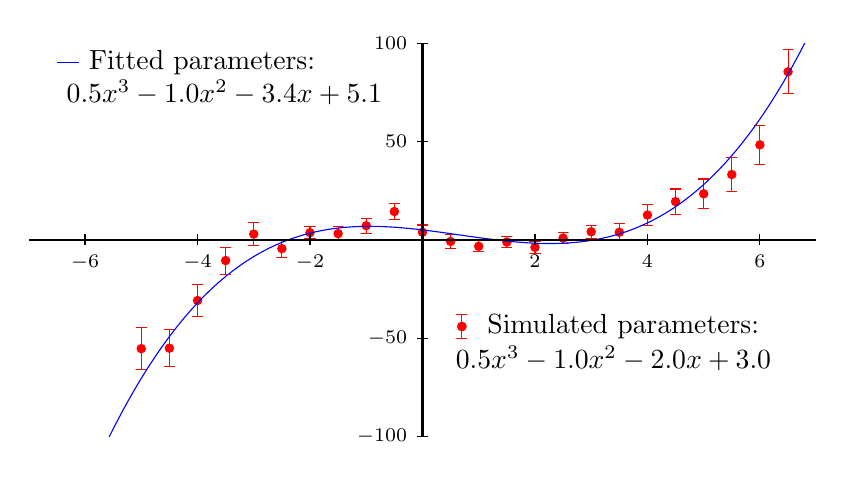
\begin{tikzpicture}
\begin{scope}[]
\pgfpathmoveto{ \pgfpointadd{\pgfpointxy {0.0} {0.0}} {\pgfpoint{0cm}{0cm}} }
\pgfpathlineto{ \pgfpointadd{\pgfpointxy {0.0} {0.0}} {\pgfpoint{10cm}{0cm}} }
\pgfpathlineto{ \pgfpointadd{\pgfpointxy {0.0} {0.0}} {\pgfpoint{10cm}{5cm}} }
\pgfpathlineto{ \pgfpointadd{\pgfpointxy {0.0} {0.0}} {\pgfpoint{0cm}{5cm}} }
\pgfpathclose
\pgfusepath{  clip, }
\begin{scope}[shift={(0.0,0.0)}]
\pgfsetxvec{\pgfpoint{0.71428573cm}{0cm}}
\pgfsetyvec{\pgfpoint{0cm}{0.025cm}}
\begin{scope}[shift={(7.0,100.0)}]
\begin{scope}[draw=red,fill=red]
\pgfpathmoveto{ \pgfpointadd{\pgfpointxy {-10.0} {-571.0535387380919}} {\pgfpoint{-2pt}{0}} }
\pgfpathlineto{ \pgfpointadd{\pgfpointxy {-10.0} {-571.0535387380919}} {\pgfpoint{2pt}{0}} }
\pgfpathlineto{ \pgfpointadd{\pgfpointxy {-10.0} {-571.0535387380919}} {\pgfpoint{0pt}{0}} }
\pgfpathlineto{ \pgfpointadd{\pgfpointxy {-10.0} {-623.095187335949}} {\pgfpoint{0pt}{0}} }
\pgfpathlineto{ \pgfpointadd{\pgfpointxy {-10.0} {-623.095187335949}} {\pgfpoint{-2pt}{0}} }
\pgfpathlineto{ \pgfpointadd{\pgfpointxy {-10.0} {-623.095187335949}} {\pgfpoint{2pt}{0}} }
\pgfusepath{ stroke, }
\node at (-10.0,-597.0743630370205) [draw=red,fill=red,circle,inner sep=0.0pt,minimum width =3.0pt,minimum height=3.0pt] {};
\end{scope}
\begin{scope}[draw=red,fill=red]
\pgfpathmoveto{ \pgfpointadd{\pgfpointxy {-9.5} {-465.4942843469761}} {\pgfpoint{-2pt}{0}} }
\pgfpathlineto{ \pgfpointadd{\pgfpointxy {-9.5} {-465.4942843469761}} {\pgfpoint{2pt}{0}} }
\pgfpathlineto{ \pgfpointadd{\pgfpointxy {-9.5} {-465.4942843469761}} {\pgfpoint{0pt}{0}} }
\pgfpathlineto{ \pgfpointadd{\pgfpointxy {-9.5} {-514.0784743698979}} {\pgfpoint{0pt}{0}} }
\pgfpathlineto{ \pgfpointadd{\pgfpointxy {-9.5} {-514.0784743698979}} {\pgfpoint{-2pt}{0}} }
\pgfpathlineto{ \pgfpointadd{\pgfpointxy {-9.5} {-514.0784743698979}} {\pgfpoint{2pt}{0}} }
\pgfusepath{ stroke, }
\node at (-9.5,-489.786379358437) [draw=red,fill=red,circle,inner sep=0.0pt,minimum width =3.0pt,minimum height=3.0pt] {};
\end{scope}
\begin{scope}[draw=red,fill=red]
\pgfpathmoveto{ \pgfpointadd{\pgfpointxy {-9.0} {-412.1044371552097}} {\pgfpoint{-2pt}{0}} }
\pgfpathlineto{ \pgfpointadd{\pgfpointxy {-9.0} {-412.1044371552097}} {\pgfpoint{2pt}{0}} }
\pgfpathlineto{ \pgfpointadd{\pgfpointxy {-9.0} {-412.1044371552097}} {\pgfpoint{0pt}{0}} }
\pgfpathlineto{ \pgfpointadd{\pgfpointxy {-9.0} {-457.3112327112828}} {\pgfpoint{0pt}{0}} }
\pgfpathlineto{ \pgfpointadd{\pgfpointxy {-9.0} {-457.3112327112828}} {\pgfpoint{-2pt}{0}} }
\pgfpathlineto{ \pgfpointadd{\pgfpointxy {-9.0} {-457.3112327112828}} {\pgfpoint{2pt}{0}} }
\pgfusepath{ stroke, }
\node at (-9.0,-434.70783493324626) [draw=red,fill=red,circle,inner sep=0.0pt,minimum width =3.0pt,minimum height=3.0pt] {};
\end{scope}
\begin{scope}[draw=red,fill=red]
\pgfpathmoveto{ \pgfpointadd{\pgfpointxy {-8.5} {-357.183759168102}} {\pgfpoint{-2pt}{0}} }
\pgfpathlineto{ \pgfpointadd{\pgfpointxy {-8.5} {-357.183759168102}} {\pgfpoint{2pt}{0}} }
\pgfpathlineto{ \pgfpointadd{\pgfpointxy {-8.5} {-357.183759168102}} {\pgfpoint{0pt}{0}} }
\pgfpathlineto{ \pgfpointadd{\pgfpointxy {-8.5} {-399.0948393426367}} {\pgfpoint{0pt}{0}} }
\pgfpathlineto{ \pgfpointadd{\pgfpointxy {-8.5} {-399.0948393426367}} {\pgfpoint{-2pt}{0}} }
\pgfpathlineto{ \pgfpointadd{\pgfpointxy {-8.5} {-399.0948393426367}} {\pgfpoint{2pt}{0}} }
\pgfusepath{ stroke, }
\node at (-8.5,-378.13929925536934) [draw=red,fill=red,circle,inner sep=0.0pt,minimum width =3.0pt,minimum height=3.0pt] {};
\end{scope}
\begin{scope}[draw=red,fill=red]
\pgfpathmoveto{ \pgfpointadd{\pgfpointxy {-8.0} {-291.87829172373085}} {\pgfpoint{-2pt}{0}} }
\pgfpathlineto{ \pgfpointadd{\pgfpointxy {-8.0} {-291.87829172373085}} {\pgfpoint{2pt}{0}} }
\pgfpathlineto{ \pgfpointadd{\pgfpointxy {-8.0} {-291.87829172373085}} {\pgfpoint{0pt}{0}} }
\pgfpathlineto{ \pgfpointadd{\pgfpointxy {-8.0} {-330.57699486952583}} {\pgfpoint{0pt}{0}} }
\pgfpathlineto{ \pgfpointadd{\pgfpointxy {-8.0} {-330.57699486952583}} {\pgfpoint{-2pt}{0}} }
\pgfpathlineto{ \pgfpointadd{\pgfpointxy {-8.0} {-330.57699486952583}} {\pgfpoint{2pt}{0}} }
\pgfusepath{ stroke, }
\node at (-8.0,-311.22764329662834) [draw=red,fill=red,circle,inner sep=0.0pt,minimum width =3.0pt,minimum height=3.0pt] {};
\end{scope}
\begin{scope}[draw=red,fill=red]
\pgfpathmoveto{ \pgfpointadd{\pgfpointxy {-7.5} {-238.3149428018001}} {\pgfpoint{-2pt}{0}} }
\pgfpathlineto{ \pgfpointadd{\pgfpointxy {-7.5} {-238.3149428018001}} {\pgfpoint{2pt}{0}} }
\pgfpathlineto{ \pgfpointadd{\pgfpointxy {-7.5} {-238.3149428018001}} {\pgfpoint{0pt}{0}} }
\pgfpathlineto{ \pgfpointadd{\pgfpointxy {-7.5} {-273.88629057157385}} {\pgfpoint{0pt}{0}} }
\pgfpathlineto{ \pgfpointadd{\pgfpointxy {-7.5} {-273.88629057157385}} {\pgfpoint{-2pt}{0}} }
\pgfpathlineto{ \pgfpointadd{\pgfpointxy {-7.5} {-273.88629057157385}} {\pgfpoint{2pt}{0}} }
\pgfusepath{ stroke, }
\node at (-7.5,-256.100616686687) [draw=red,fill=red,circle,inner sep=0.0pt,minimum width =3.0pt,minimum height=3.0pt] {};
\end{scope}
\begin{scope}[draw=red,fill=red]
\pgfpathmoveto{ \pgfpointadd{\pgfpointxy {-7.0} {-202.29808062975653}} {\pgfpoint{-2pt}{0}} }
\pgfpathlineto{ \pgfpointadd{\pgfpointxy {-7.0} {-202.29808062975653}} {\pgfpoint{2pt}{0}} }
\pgfpathlineto{ \pgfpointadd{\pgfpointxy {-7.0} {-202.29808062975653}} {\pgfpoint{0pt}{0}} }
\pgfpathlineto{ \pgfpointadd{\pgfpointxy {-7.0} {-234.82876586513075}} {\pgfpoint{0pt}{0}} }
\pgfpathlineto{ \pgfpointadd{\pgfpointxy {-7.0} {-234.82876586513075}} {\pgfpoint{-2pt}{0}} }
\pgfpathlineto{ \pgfpointadd{\pgfpointxy {-7.0} {-234.82876586513075}} {\pgfpoint{2pt}{0}} }
\pgfusepath{ stroke, }
\node at (-7.0,-218.56342324744364) [draw=red,fill=red,circle,inner sep=0.0pt,minimum width =3.0pt,minimum height=3.0pt] {};
\end{scope}
\begin{scope}[draw=red,fill=red]
\pgfpathmoveto{ \pgfpointadd{\pgfpointxy {-6.5} {-145.7322270733457}} {\pgfpoint{-2pt}{0}} }
\pgfpathlineto{ \pgfpointadd{\pgfpointxy {-6.5} {-145.7322270733457}} {\pgfpoint{2pt}{0}} }
\pgfpathlineto{ \pgfpointadd{\pgfpointxy {-6.5} {-145.7322270733457}} {\pgfpoint{0pt}{0}} }
\pgfpathlineto{ \pgfpointadd{\pgfpointxy {-6.5} {-175.31053819820306}} {\pgfpoint{0pt}{0}} }
\pgfpathlineto{ \pgfpointadd{\pgfpointxy {-6.5} {-175.31053819820306}} {\pgfpoint{-2pt}{0}} }
\pgfpathlineto{ \pgfpointadd{\pgfpointxy {-6.5} {-175.31053819820306}} {\pgfpoint{2pt}{0}} }
\pgfusepath{ stroke, }
\node at (-6.5,-160.5213826357744) [draw=red,fill=red,circle,inner sep=0.0pt,minimum width =3.0pt,minimum height=3.0pt] {};
\end{scope}
\begin{scope}[draw=red,fill=red]
\pgfpathmoveto{ \pgfpointadd{\pgfpointxy {-6.0} {-109.22115465709189}} {\pgfpoint{-2pt}{0}} }
\pgfpathlineto{ \pgfpointadd{\pgfpointxy {-6.0} {-109.22115465709189}} {\pgfpoint{2pt}{0}} }
\pgfpathlineto{ \pgfpointadd{\pgfpointxy {-6.0} {-109.22115465709189}} {\pgfpoint{0pt}{0}} }
\pgfpathlineto{ \pgfpointadd{\pgfpointxy {-6.0} {-135.93678804029298}} {\pgfpoint{0pt}{0}} }
\pgfpathlineto{ \pgfpointadd{\pgfpointxy {-6.0} {-135.93678804029298}} {\pgfpoint{-2pt}{0}} }
\pgfpathlineto{ \pgfpointadd{\pgfpointxy {-6.0} {-135.93678804029298}} {\pgfpoint{2pt}{0}} }
\pgfusepath{ stroke, }
\node at (-6.0,-122.57897134869243) [draw=red,fill=red,circle,inner sep=0.0pt,minimum width =3.0pt,minimum height=3.0pt] {};
\end{scope}
\begin{scope}[draw=red,fill=red]
\pgfpathmoveto{ \pgfpointadd{\pgfpointxy {-5.5} {-109.25232418508995}} {\pgfpoint{-2pt}{0}} }
\pgfpathlineto{ \pgfpointadd{\pgfpointxy {-5.5} {-109.25232418508995}} {\pgfpoint{2pt}{0}} }
\pgfpathlineto{ \pgfpointadd{\pgfpointxy {-5.5} {-109.25232418508995}} {\pgfpoint{0pt}{0}} }
\pgfpathlineto{ \pgfpointadd{\pgfpointxy {-5.5} {-133.19599486026908}} {\pgfpoint{0pt}{0}} }
\pgfpathlineto{ \pgfpointadd{\pgfpointxy {-5.5} {-133.19599486026908}} {\pgfpoint{-2pt}{0}} }
\pgfpathlineto{ \pgfpointadd{\pgfpointxy {-5.5} {-133.19599486026908}} {\pgfpoint{2pt}{0}} }
\pgfusepath{ stroke, }
\node at (-5.5,-121.22415952267951) [draw=red,fill=red,circle,inner sep=0.0pt,minimum width =3.0pt,minimum height=3.0pt] {};
\end{scope}
\begin{scope}[draw=red,fill=red]
\pgfpathmoveto{ \pgfpointadd{\pgfpointxy {-5.0} {-44.62018863682962}} {\pgfpoint{-2pt}{0}} }
\pgfpathlineto{ \pgfpointadd{\pgfpointxy {-5.0} {-44.62018863682962}} {\pgfpoint{2pt}{0}} }
\pgfpathlineto{ \pgfpointadd{\pgfpointxy {-5.0} {-44.62018863682962}} {\pgfpoint{0pt}{0}} }
\pgfpathlineto{ \pgfpointadd{\pgfpointxy {-5.0} {-65.88286513846168}} {\pgfpoint{0pt}{0}} }
\pgfpathlineto{ \pgfpointadd{\pgfpointxy {-5.0} {-65.88286513846168}} {\pgfpoint{-2pt}{0}} }
\pgfpathlineto{ \pgfpointadd{\pgfpointxy {-5.0} {-65.88286513846168}} {\pgfpoint{2pt}{0}} }
\pgfusepath{ stroke, }
\node at (-5.0,-55.25152688764565) [draw=red,fill=red,circle,inner sep=0.0pt,minimum width =3.0pt,minimum height=3.0pt] {};
\end{scope}
\begin{scope}[draw=red,fill=red]
\pgfpathmoveto{ \pgfpointadd{\pgfpointxy {-4.5} {-45.66786522760035}} {\pgfpoint{-2pt}{0}} }
\pgfpathlineto{ \pgfpointadd{\pgfpointxy {-4.5} {-45.66786522760035}} {\pgfpoint{2pt}{0}} }
\pgfpathlineto{ \pgfpointadd{\pgfpointxy {-4.5} {-45.66786522760035}} {\pgfpoint{0pt}{0}} }
\pgfpathlineto{ \pgfpointadd{\pgfpointxy {-4.5} {-64.33926597872156}} {\pgfpoint{0pt}{0}} }
\pgfpathlineto{ \pgfpointadd{\pgfpointxy {-4.5} {-64.33926597872156}} {\pgfpoint{-2pt}{0}} }
\pgfpathlineto{ \pgfpointadd{\pgfpointxy {-4.5} {-64.33926597872156}} {\pgfpoint{2pt}{0}} }
\pgfusepath{ stroke, }
\node at (-4.5,-55.00356560316096) [draw=red,fill=red,circle,inner sep=0.0pt,minimum width =3.0pt,minimum height=3.0pt] {};
\end{scope}
\begin{scope}[draw=red,fill=red]
\pgfpathmoveto{ \pgfpointadd{\pgfpointxy {-4.0} {-22.71518997590085}} {\pgfpoint{-2pt}{0}} }
\pgfpathlineto{ \pgfpointadd{\pgfpointxy {-4.0} {-22.71518997590085}} {\pgfpoint{2pt}{0}} }
\pgfpathlineto{ \pgfpointadd{\pgfpointxy {-4.0} {-22.71518997590085}} {\pgfpoint{0pt}{0}} }
\pgfpathlineto{ \pgfpointadd{\pgfpointxy {-4.0} {-38.880715036497286}} {\pgfpoint{0pt}{0}} }
\pgfpathlineto{ \pgfpointadd{\pgfpointxy {-4.0} {-38.880715036497286}} {\pgfpoint{-2pt}{0}} }
\pgfpathlineto{ \pgfpointadd{\pgfpointxy {-4.0} {-38.880715036497286}} {\pgfpoint{2pt}{0}} }
\pgfusepath{ stroke, }
\node at (-4.0,-30.797952506199067) [draw=red,fill=red,circle,inner sep=0.0pt,minimum width =3.0pt,minimum height=3.0pt] {};
\end{scope}
\begin{scope}[draw=red,fill=red]
\pgfpathmoveto{ \pgfpointadd{\pgfpointxy {-3.5} {-3.623367622026165}} {\pgfpoint{-2pt}{0}} }
\pgfpathlineto{ \pgfpointadd{\pgfpointxy {-3.5} {-3.623367622026165}} {\pgfpoint{2pt}{0}} }
\pgfpathlineto{ \pgfpointadd{\pgfpointxy {-3.5} {-3.623367622026165}} {\pgfpoint{0pt}{0}} }
\pgfpathlineto{ \pgfpointadd{\pgfpointxy {-3.5} {-17.357328788992056}} {\pgfpoint{0pt}{0}} }
\pgfpathlineto{ \pgfpointadd{\pgfpointxy {-3.5} {-17.357328788992056}} {\pgfpoint{-2pt}{0}} }
\pgfpathlineto{ \pgfpointadd{\pgfpointxy {-3.5} {-17.357328788992056}} {\pgfpoint{2pt}{0}} }
\pgfusepath{ stroke, }
\node at (-3.5,-10.490348205509111) [draw=red,fill=red,circle,inner sep=0.0pt,minimum width =3.0pt,minimum height=3.0pt] {};
\end{scope}
\begin{scope}[draw=red,fill=red]
\pgfpathmoveto{ \pgfpointadd{\pgfpointxy {-3.0} {8.659705441078653}} {\pgfpoint{-2pt}{0}} }
\pgfpathlineto{ \pgfpointadd{\pgfpointxy {-3.0} {8.659705441078653}} {\pgfpoint{2pt}{0}} }
\pgfpathlineto{ \pgfpointadd{\pgfpointxy {-3.0} {8.659705441078653}} {\pgfpoint{0pt}{0}} }
\pgfpathlineto{ \pgfpointadd{\pgfpointxy {-3.0} {-2.688763787270882}} {\pgfpoint{0pt}{0}} }
\pgfpathlineto{ \pgfpointadd{\pgfpointxy {-3.0} {-2.688763787270882}} {\pgfpoint{-2pt}{0}} }
\pgfpathlineto{ \pgfpointadd{\pgfpointxy {-3.0} {-2.688763787270882}} {\pgfpoint{2pt}{0}} }
\pgfusepath{ stroke, }
\node at (-3.0,2.985470826903885) [draw=red,fill=red,circle,inner sep=0.0pt,minimum width =3.0pt,minimum height=3.0pt] {};
\end{scope}
\begin{scope}[draw=red,fill=red]
\pgfpathmoveto{ \pgfpointadd{\pgfpointxy {-2.5} {0.03452070884278502}} {\pgfpoint{-2pt}{0}} }
\pgfpathlineto{ \pgfpointadd{\pgfpointxy {-2.5} {0.03452070884278502}} {\pgfpoint{2pt}{0}} }
\pgfpathlineto{ \pgfpointadd{\pgfpointxy {-2.5} {0.03452070884278502}} {\pgfpoint{0pt}{0}} }
\pgfpathlineto{ \pgfpointadd{\pgfpointxy {-2.5} {-8.889908192055266}} {\pgfpoint{0pt}{0}} }
\pgfpathlineto{ \pgfpointadd{\pgfpointxy {-2.5} {-8.889908192055266}} {\pgfpoint{-2pt}{0}} }
\pgfpathlineto{ \pgfpointadd{\pgfpointxy {-2.5} {-8.889908192055266}} {\pgfpoint{2pt}{0}} }
\pgfusepath{ stroke, }
\node at (-2.5,-4.427693741606241) [draw=red,fill=red,circle,inner sep=0.0pt,minimum width =3.0pt,minimum height=3.0pt] {};
\end{scope}
\begin{scope}[draw=red,fill=red]
\pgfpathmoveto{ \pgfpointadd{\pgfpointxy {-2.0} {6.691469768324479}} {\pgfpoint{-2pt}{0}} }
\pgfpathlineto{ \pgfpointadd{\pgfpointxy {-2.0} {6.691469768324479}} {\pgfpoint{2pt}{0}} }
\pgfpathlineto{ \pgfpointadd{\pgfpointxy {-2.0} {6.691469768324479}} {\pgfpoint{0pt}{0}} }
\pgfpathlineto{ \pgfpointadd{\pgfpointxy {-2.0} {0.6914697683244793}} {\pgfpoint{0pt}{0}} }
\pgfpathlineto{ \pgfpointadd{\pgfpointxy {-2.0} {0.6914697683244793}} {\pgfpoint{-2pt}{0}} }
\pgfpathlineto{ \pgfpointadd{\pgfpointxy {-2.0} {0.6914697683244793}} {\pgfpoint{2pt}{0}} }
\pgfusepath{ stroke, }
\node at (-2.0,3.6914697683244793) [draw=red,fill=red,circle,inner sep=0.0pt,minimum width =3.0pt,minimum height=3.0pt] {};
\end{scope}
\begin{scope}[draw=red,fill=red]
\pgfpathmoveto{ \pgfpointadd{\pgfpointxy {-1.5} {6.642849316210677}} {\pgfpoint{-2pt}{0}} }
\pgfpathlineto{ \pgfpointadd{\pgfpointxy {-1.5} {6.642849316210677}} {\pgfpoint{2pt}{0}} }
\pgfpathlineto{ \pgfpointadd{\pgfpointxy {-1.5} {6.642849316210677}} {\pgfpoint{0pt}{0}} }
\pgfpathlineto{ \pgfpointadd{\pgfpointxy {-1.5} {-0.2294320070583371}} {\pgfpoint{0pt}{0}} }
\pgfpathlineto{ \pgfpointadd{\pgfpointxy {-1.5} {-0.2294320070583371}} {\pgfpoint{-2pt}{0}} }
\pgfpathlineto{ \pgfpointadd{\pgfpointxy {-1.5} {-0.2294320070583371}} {\pgfpoint{2pt}{0}} }
\pgfusepath{ stroke, }
\node at (-1.5,3.20670865457617) [draw=red,fill=red,circle,inner sep=0.0pt,minimum width =3.0pt,minimum height=3.0pt] {};
\end{scope}
\begin{scope}[draw=red,fill=red]
\pgfpathmoveto{ \pgfpointadd{\pgfpointxy {-1.0} {11.107898214064939}} {\pgfpoint{-2pt}{0}} }
\pgfpathlineto{ \pgfpointadd{\pgfpointxy {-1.0} {11.107898214064939}} {\pgfpoint{2pt}{0}} }
\pgfpathlineto{ \pgfpointadd{\pgfpointxy {-1.0} {11.107898214064939}} {\pgfpoint{0pt}{0}} }
\pgfpathlineto{ \pgfpointadd{\pgfpointxy {-1.0} {3.3662408272909987}} {\pgfpoint{0pt}{0}} }
\pgfpathlineto{ \pgfpointadd{\pgfpointxy {-1.0} {3.3662408272909987}} {\pgfpoint{-2pt}{0}} }
\pgfpathlineto{ \pgfpointadd{\pgfpointxy {-1.0} {3.3662408272909987}} {\pgfpoint{2pt}{0}} }
\pgfusepath{ stroke, }
\node at (-1.0,7.237069520677969) [draw=red,fill=red,circle,inner sep=0.0pt,minimum width =3.0pt,minimum height=3.0pt] {};
\end{scope}
\begin{scope}[draw=red,fill=red]
\pgfpathmoveto{ \pgfpointadd{\pgfpointxy {-0.5} {18.362804815403905}} {\pgfpoint{-2pt}{0}} }
\pgfpathlineto{ \pgfpointadd{\pgfpointxy {-0.5} {18.362804815403905}} {\pgfpoint{2pt}{0}} }
\pgfpathlineto{ \pgfpointadd{\pgfpointxy {-0.5} {18.362804815403905}} {\pgfpoint{0pt}{0}} }
\pgfpathlineto{ \pgfpointadd{\pgfpointxy {-0.5} {10.522231941469602}} {\pgfpoint{0pt}{0}} }
\pgfpathlineto{ \pgfpointadd{\pgfpointxy {-0.5} {10.522231941469602}} {\pgfpoint{-2pt}{0}} }
\pgfpathlineto{ \pgfpointadd{\pgfpointxy {-0.5} {10.522231941469602}} {\pgfpoint{2pt}{0}} }
\pgfusepath{ stroke, }
\node at (-0.5,14.442518378436754) [draw=red,fill=red,circle,inner sep=0.0pt,minimum width =3.0pt,minimum height=3.0pt] {};
\end{scope}
\begin{scope}[draw=red,fill=red]
\pgfpathmoveto{ \pgfpointadd{\pgfpointxy {0.0} {7.612007955975413}} {\pgfpoint{-2pt}{0}} }
\pgfpathlineto{ \pgfpointadd{\pgfpointxy {0.0} {7.612007955975413}} {\pgfpoint{2pt}{0}} }
\pgfpathlineto{ \pgfpointadd{\pgfpointxy {0.0} {7.612007955975413}} {\pgfpoint{0pt}{0}} }
\pgfpathlineto{ \pgfpointadd{\pgfpointxy {0.0} {0.14790634083765797}} {\pgfpoint{0pt}{0}} }
\pgfpathlineto{ \pgfpointadd{\pgfpointxy {0.0} {0.14790634083765797}} {\pgfpoint{-2pt}{0}} }
\pgfpathlineto{ \pgfpointadd{\pgfpointxy {0.0} {0.14790634083765797}} {\pgfpoint{2pt}{0}} }
\pgfusepath{ stroke, }
\node at (0.0,3.879957148406535) [draw=red,fill=red,circle,inner sep=0.0pt,minimum width =3.0pt,minimum height=3.0pt] {};
\end{scope}
\begin{scope}[draw=red,fill=red]
\pgfpathmoveto{ \pgfpointadd{\pgfpointxy {0.5} {2.5683907793851475}} {\pgfpoint{-2pt}{0}} }
\pgfpathlineto{ \pgfpointadd{\pgfpointxy {0.5} {2.5683907793851475}} {\pgfpoint{2pt}{0}} }
\pgfpathlineto{ \pgfpointadd{\pgfpointxy {0.5} {2.5683907793851475}} {\pgfpoint{0pt}{0}} }
\pgfpathlineto{ \pgfpointadd{\pgfpointxy {0.5} {-4.124191624182105}} {\pgfpoint{0pt}{0}} }
\pgfpathlineto{ \pgfpointadd{\pgfpointxy {0.5} {-4.124191624182105}} {\pgfpoint{-2pt}{0}} }
\pgfpathlineto{ \pgfpointadd{\pgfpointxy {0.5} {-4.124191624182105}} {\pgfpoint{2pt}{0}} }
\pgfusepath{ stroke, }
\node at (0.5,-0.7779004223984787) [draw=red,fill=red,circle,inner sep=0.0pt,minimum width =3.0pt,minimum height=3.0pt] {};
\end{scope}
\begin{scope}[draw=red,fill=red]
\pgfpathmoveto{ \pgfpointadd{\pgfpointxy {1.0} {-0.5092360123617312}} {\pgfpoint{-2pt}{0}} }
\pgfpathlineto{ \pgfpointadd{\pgfpointxy {1.0} {-0.5092360123617312}} {\pgfpoint{2pt}{0}} }
\pgfpathlineto{ \pgfpointadd{\pgfpointxy {1.0} {-0.5092360123617312}} {\pgfpoint{0pt}{0}} }
\pgfpathlineto{ \pgfpointadd{\pgfpointxy {1.0} {-5.923449574734827}} {\pgfpoint{0pt}{0}} }
\pgfpathlineto{ \pgfpointadd{\pgfpointxy {1.0} {-5.923449574734827}} {\pgfpoint{-2pt}{0}} }
\pgfpathlineto{ \pgfpointadd{\pgfpointxy {1.0} {-5.923449574734827}} {\pgfpoint{2pt}{0}} }
\pgfusepath{ stroke, }
\node at (1.0,-3.2163427935482787) [draw=red,fill=red,circle,inner sep=0.0pt,minimum width =3.0pt,minimum height=3.0pt] {};
\end{scope}
\begin{scope}[draw=red,fill=red]
\pgfpathmoveto{ \pgfpointadd{\pgfpointxy {1.5} {1.6701722960789132}} {\pgfpoint{-2pt}{0}} }
\pgfpathlineto{ \pgfpointadd{\pgfpointxy {1.5} {1.6701722960789132}} {\pgfpoint{2pt}{0}} }
\pgfpathlineto{ \pgfpointadd{\pgfpointxy {1.5} {1.6701722960789132}} {\pgfpoint{0pt}{0}} }
\pgfpathlineto{ \pgfpointadd{\pgfpointxy {1.5} {-3.8298277039210866}} {\pgfpoint{0pt}{0}} }
\pgfpathlineto{ \pgfpointadd{\pgfpointxy {1.5} {-3.8298277039210866}} {\pgfpoint{-2pt}{0}} }
\pgfpathlineto{ \pgfpointadd{\pgfpointxy {1.5} {-3.8298277039210866}} {\pgfpoint{2pt}{0}} }
\pgfusepath{ stroke, }
\node at (1.5,-1.0798277039210868) [draw=red,fill=red,circle,inner sep=0.0pt,minimum width =3.0pt,minimum height=3.0pt] {};
\end{scope}
\begin{scope}[draw=red,fill=red]
\pgfpathmoveto{ \pgfpointadd{\pgfpointxy {2.0} {-0.7755617046804377}} {\pgfpoint{-2pt}{0}} }
\pgfpathlineto{ \pgfpointadd{\pgfpointxy {2.0} {-0.7755617046804377}} {\pgfpoint{2pt}{0}} }
\pgfpathlineto{ \pgfpointadd{\pgfpointxy {2.0} {-0.7755617046804377}} {\pgfpoint{0pt}{0}} }
\pgfpathlineto{ \pgfpointadd{\pgfpointxy {2.0} {-6.775561704680438}} {\pgfpoint{0pt}{0}} }
\pgfpathlineto{ \pgfpointadd{\pgfpointxy {2.0} {-6.775561704680438}} {\pgfpoint{-2pt}{0}} }
\pgfpathlineto{ \pgfpointadd{\pgfpointxy {2.0} {-6.775561704680438}} {\pgfpoint{2pt}{0}} }
\pgfusepath{ stroke, }
\node at (2.0,-3.7755617046804377) [draw=red,fill=red,circle,inner sep=0.0pt,minimum width =3.0pt,minimum height=3.0pt] {};
\end{scope}
\begin{scope}[draw=red,fill=red]
\pgfpathmoveto{ \pgfpointadd{\pgfpointxy {2.5} {3.599233927702615}} {\pgfpoint{-2pt}{0}} }
\pgfpathlineto{ \pgfpointadd{\pgfpointxy {2.5} {3.599233927702615}} {\pgfpoint{2pt}{0}} }
\pgfpathlineto{ \pgfpointadd{\pgfpointxy {2.5} {3.599233927702615}} {\pgfpoint{0pt}{0}} }
\pgfpathlineto{ \pgfpointadd{\pgfpointxy {2.5} {-1.72364172782968}} {\pgfpoint{0pt}{0}} }
\pgfpathlineto{ \pgfpointadd{\pgfpointxy {2.5} {-1.72364172782968}} {\pgfpoint{-2pt}{0}} }
\pgfpathlineto{ \pgfpointadd{\pgfpointxy {2.5} {-1.72364172782968}} {\pgfpoint{2pt}{0}} }
\pgfusepath{ stroke, }
\node at (2.5,0.9377960999364674) [draw=red,fill=red,circle,inner sep=0.0pt,minimum width =3.0pt,minimum height=3.0pt] {};
\end{scope}
\begin{scope}[draw=red,fill=red]
\pgfpathmoveto{ \pgfpointadd{\pgfpointxy {3.0} {7.3753525624062775}} {\pgfpoint{-2pt}{0}} }
\pgfpathlineto{ \pgfpointadd{\pgfpointxy {3.0} {7.3753525624062775}} {\pgfpoint{2pt}{0}} }
\pgfpathlineto{ \pgfpointadd{\pgfpointxy {3.0} {7.3753525624062775}} {\pgfpoint{0pt}{0}} }
\pgfpathlineto{ \pgfpointadd{\pgfpointxy {3.0} {0.9258628196231}} {\pgfpoint{0pt}{0}} }
\pgfpathlineto{ \pgfpointadd{\pgfpointxy {3.0} {0.9258628196231}} {\pgfpoint{-2pt}{0}} }
\pgfpathlineto{ \pgfpointadd{\pgfpointxy {3.0} {0.9258628196231}} {\pgfpoint{2pt}{0}} }
\pgfusepath{ stroke, }
\node at (3.0,4.150607691014689) [draw=red,fill=red,circle,inner sep=0.0pt,minimum width =3.0pt,minimum height=3.0pt] {};
\end{scope}
\begin{scope}[draw=red,fill=red]
\pgfpathmoveto{ \pgfpointadd{\pgfpointxy {3.5} {8.180402037547292}} {\pgfpoint{-2pt}{0}} }
\pgfpathlineto{ \pgfpointadd{\pgfpointxy {3.5} {8.180402037547292}} {\pgfpoint{2pt}{0}} }
\pgfpathlineto{ \pgfpointadd{\pgfpointxy {3.5} {8.180402037547292}} {\pgfpoint{0pt}{0}} }
\pgfpathlineto{ \pgfpointadd{\pgfpointxy {3.5} {-0.37481475202485726}} {\pgfpoint{0pt}{0}} }
\pgfpathlineto{ \pgfpointadd{\pgfpointxy {3.5} {-0.37481475202485726}} {\pgfpoint{-2pt}{0}} }
\pgfpathlineto{ \pgfpointadd{\pgfpointxy {3.5} {-0.37481475202485726}} {\pgfpoint{2pt}{0}} }
\pgfusepath{ stroke, }
\node at (3.5,3.9027936427612175) [draw=red,fill=red,circle,inner sep=0.0pt,minimum width =3.0pt,minimum height=3.0pt] {};
\end{scope}
\begin{scope}[draw=red,fill=red]
\pgfpathmoveto{ \pgfpointadd{\pgfpointxy {4.0} {17.985284457749778}} {\pgfpoint{-2pt}{0}} }
\pgfpathlineto{ \pgfpointadd{\pgfpointxy {4.0} {17.985284457749778}} {\pgfpoint{2pt}{0}} }
\pgfpathlineto{ \pgfpointadd{\pgfpointxy {4.0} {17.985284457749778}} {\pgfpoint{0pt}{0}} }
\pgfpathlineto{ \pgfpointadd{\pgfpointxy {4.0} {7.352034877038976}} {\pgfpoint{0pt}{0}} }
\pgfpathlineto{ \pgfpointadd{\pgfpointxy {4.0} {7.352034877038976}} {\pgfpoint{-2pt}{0}} }
\pgfpathlineto{ \pgfpointadd{\pgfpointxy {4.0} {7.352034877038976}} {\pgfpoint{2pt}{0}} }
\pgfusepath{ stroke, }
\node at (4.0,12.668659667394376) [draw=red,fill=red,circle,inner sep=0.0pt,minimum width =3.0pt,minimum height=3.0pt] {};
\end{scope}
\begin{scope}[draw=red,fill=red]
\pgfpathmoveto{ \pgfpointadd{\pgfpointxy {4.5} {25.865344976413038}} {\pgfpoint{-2pt}{0}} }
\pgfpathlineto{ \pgfpointadd{\pgfpointxy {4.5} {25.865344976413038}} {\pgfpoint{2pt}{0}} }
\pgfpathlineto{ \pgfpointadd{\pgfpointxy {4.5} {25.865344976413038}} {\pgfpoint{0pt}{0}} }
\pgfpathlineto{ \pgfpointadd{\pgfpointxy {4.5} {13.076147060789562}} {\pgfpoint{0pt}{0}} }
\pgfpathlineto{ \pgfpointadd{\pgfpointxy {4.5} {13.076147060789562}} {\pgfpoint{-2pt}{0}} }
\pgfpathlineto{ \pgfpointadd{\pgfpointxy {4.5} {13.076147060789562}} {\pgfpoint{2pt}{0}} }
\pgfusepath{ stroke, }
\node at (4.5,19.4707460186013) [draw=red,fill=red,circle,inner sep=0.0pt,minimum width =3.0pt,minimum height=3.0pt] {};
\end{scope}
\begin{scope}[draw=red,fill=red]
\pgfpathmoveto{ \pgfpointadd{\pgfpointxy {5.0} {30.966184447206345}} {\pgfpoint{-2pt}{0}} }
\pgfpathlineto{ \pgfpointadd{\pgfpointxy {5.0} {30.966184447206345}} {\pgfpoint{2pt}{0}} }
\pgfpathlineto{ \pgfpointadd{\pgfpointxy {5.0} {30.966184447206345}} {\pgfpoint{0pt}{0}} }
\pgfpathlineto{ \pgfpointadd{\pgfpointxy {5.0} {15.920823430019084}} {\pgfpoint{0pt}{0}} }
\pgfpathlineto{ \pgfpointadd{\pgfpointxy {5.0} {15.920823430019084}} {\pgfpoint{-2pt}{0}} }
\pgfpathlineto{ \pgfpointadd{\pgfpointxy {5.0} {15.920823430019084}} {\pgfpoint{2pt}{0}} }
\pgfusepath{ stroke, }
\node at (5.0,23.443503938612714) [draw=red,fill=red,circle,inner sep=0.0pt,minimum width =3.0pt,minimum height=3.0pt] {};
\end{scope}
\begin{scope}[draw=red,fill=red]
\pgfpathmoveto{ \pgfpointadd{\pgfpointxy {5.5} {41.93279338298936}} {\pgfpoint{-2pt}{0}} }
\pgfpathlineto{ \pgfpointadd{\pgfpointxy {5.5} {41.93279338298936}} {\pgfpoint{2pt}{0}} }
\pgfpathlineto{ \pgfpointadd{\pgfpointxy {5.5} {41.93279338298936}} {\pgfpoint{0pt}{0}} }
\pgfpathlineto{ \pgfpointadd{\pgfpointxy {5.5} {24.52570570519744}} {\pgfpoint{0pt}{0}} }
\pgfpathlineto{ \pgfpointadd{\pgfpointxy {5.5} {24.52570570519744}} {\pgfpoint{-2pt}{0}} }
\pgfpathlineto{ \pgfpointadd{\pgfpointxy {5.5} {24.52570570519744}} {\pgfpoint{2pt}{0}} }
\pgfusepath{ stroke, }
\node at (5.5,33.2292495440934) [draw=red,fill=red,circle,inner sep=0.0pt,minimum width =3.0pt,minimum height=3.0pt] {};
\end{scope}
\begin{scope}[draw=red,fill=red]
\pgfpathmoveto{ \pgfpointadd{\pgfpointxy {6.0} {58.24963967593858}} {\pgfpoint{-2pt}{0}} }
\pgfpathlineto{ \pgfpointadd{\pgfpointxy {6.0} {58.24963967593858}} {\pgfpoint{2pt}{0}} }
\pgfpathlineto{ \pgfpointadd{\pgfpointxy {6.0} {58.24963967593858}} {\pgfpoint{0pt}{0}} }
\pgfpathlineto{ \pgfpointadd{\pgfpointxy {6.0} {38.375131809551036}} {\pgfpoint{0pt}{0}} }
\pgfpathlineto{ \pgfpointadd{\pgfpointxy {6.0} {38.375131809551036}} {\pgfpoint{-2pt}{0}} }
\pgfpathlineto{ \pgfpointadd{\pgfpointxy {6.0} {38.375131809551036}} {\pgfpoint{2pt}{0}} }
\pgfusepath{ stroke, }
\node at (6.0,48.31238574274481) [draw=red,fill=red,circle,inner sep=0.0pt,minimum width =3.0pt,minimum height=3.0pt] {};
\end{scope}
\begin{scope}[draw=red,fill=red]
\pgfpathmoveto{ \pgfpointadd{\pgfpointxy {6.5} {96.67541812918063}} {\pgfpoint{-2pt}{0}} }
\pgfpathlineto{ \pgfpointadd{\pgfpointxy {6.5} {96.67541812918063}} {\pgfpoint{2pt}{0}} }
\pgfpathlineto{ \pgfpointadd{\pgfpointxy {6.5} {96.67541812918063}} {\pgfpoint{0pt}{0}} }
\pgfpathlineto{ \pgfpointadd{\pgfpointxy {6.5} {74.22955138348391}} {\pgfpoint{0pt}{0}} }
\pgfpathlineto{ \pgfpointadd{\pgfpointxy {6.5} {74.22955138348391}} {\pgfpoint{-2pt}{0}} }
\pgfpathlineto{ \pgfpointadd{\pgfpointxy {6.5} {74.22955138348391}} {\pgfpoint{2pt}{0}} }
\pgfusepath{ stroke, }
\node at (6.5,85.45248475633227) [draw=red,fill=red,circle,inner sep=0.0pt,minimum width =3.0pt,minimum height=3.0pt] {};
\end{scope}
\begin{scope}[draw=red,fill=red]
\pgfpathmoveto{ \pgfpointadd{\pgfpointxy {7.0} {150.98758050732656}} {\pgfpoint{-2pt}{0}} }
\pgfpathlineto{ \pgfpointadd{\pgfpointxy {7.0} {150.98758050732656}} {\pgfpoint{2pt}{0}} }
\pgfpathlineto{ \pgfpointadd{\pgfpointxy {7.0} {150.98758050732656}} {\pgfpoint{0pt}{0}} }
\pgfpathlineto{ \pgfpointadd{\pgfpointxy {7.0} {125.86886842538368}} {\pgfpoint{0pt}{0}} }
\pgfpathlineto{ \pgfpointadd{\pgfpointxy {7.0} {125.86886842538368}} {\pgfpoint{-2pt}{0}} }
\pgfpathlineto{ \pgfpointadd{\pgfpointxy {7.0} {125.86886842538368}} {\pgfpoint{2pt}{0}} }
\pgfusepath{ stroke, }
\node at (7.0,138.42822446635512) [draw=red,fill=red,circle,inner sep=0.0pt,minimum width =3.0pt,minimum height=3.0pt] {};
\end{scope}
\begin{scope}[draw=red,fill=red]
\pgfpathmoveto{ \pgfpointadd{\pgfpointxy {7.5} {137.62912541707732}} {\pgfpoint{-2pt}{0}} }
\pgfpathlineto{ \pgfpointadd{\pgfpointxy {7.5} {137.62912541707732}} {\pgfpoint{2pt}{0}} }
\pgfpathlineto{ \pgfpointadd{\pgfpointxy {7.5} {137.62912541707732}} {\pgfpoint{0pt}{0}} }
\pgfpathlineto{ \pgfpointadd{\pgfpointxy {7.5} {109.73875078627674}} {\pgfpoint{0pt}{0}} }
\pgfpathlineto{ \pgfpointadd{\pgfpointxy {7.5} {109.73875078627674}} {\pgfpoint{-2pt}{0}} }
\pgfpathlineto{ \pgfpointadd{\pgfpointxy {7.5} {109.73875078627674}} {\pgfpoint{2pt}{0}} }
\pgfusepath{ stroke, }
\node at (7.5,123.68393810167703) [draw=red,fill=red,circle,inner sep=0.0pt,minimum width =3.0pt,minimum height=3.0pt] {};
\end{scope}
\begin{scope}[draw=red,fill=red]
\pgfpathmoveto{ \pgfpointadd{\pgfpointxy {8.0} {201.411347251231}} {\pgfpoint{-2pt}{0}} }
\pgfpathlineto{ \pgfpointadd{\pgfpointxy {8.0} {201.411347251231}} {\pgfpoint{2pt}{0}} }
\pgfpathlineto{ \pgfpointadd{\pgfpointxy {8.0} {201.411347251231}} {\pgfpoint{0pt}{0}} }
\pgfpathlineto{ \pgfpointadd{\pgfpointxy {8.0} {170.65317093071172}} {\pgfpoint{0pt}{0}} }
\pgfpathlineto{ \pgfpointadd{\pgfpointxy {8.0} {170.65317093071172}} {\pgfpoint{-2pt}{0}} }
\pgfpathlineto{ \pgfpointadd{\pgfpointxy {8.0} {170.65317093071172}} {\pgfpoint{2pt}{0}} }
\pgfusepath{ stroke, }
\node at (8.0,186.03225909097137) [draw=red,fill=red,circle,inner sep=0.0pt,minimum width =3.0pt,minimum height=3.0pt] {};
\end{scope}
\begin{scope}[draw=red,fill=red]
\pgfpathmoveto{ \pgfpointadd{\pgfpointxy {8.5} {240.7691872656242}} {\pgfpoint{-2pt}{0}} }
\pgfpathlineto{ \pgfpointadd{\pgfpointxy {8.5} {240.7691872656242}} {\pgfpoint{2pt}{0}} }
\pgfpathlineto{ \pgfpointadd{\pgfpointxy {8.5} {240.7691872656242}} {\pgfpoint{0pt}{0}} }
\pgfpathlineto{ \pgfpointadd{\pgfpointxy {8.5} {207.04966506219702}} {\pgfpoint{0pt}{0}} }
\pgfpathlineto{ \pgfpointadd{\pgfpointxy {8.5} {207.04966506219702}} {\pgfpoint{-2pt}{0}} }
\pgfpathlineto{ \pgfpointadd{\pgfpointxy {8.5} {207.04966506219702}} {\pgfpoint{2pt}{0}} }
\pgfusepath{ stroke, }
\node at (8.5,223.9094261639106) [draw=red,fill=red,circle,inner sep=0.0pt,minimum width =3.0pt,minimum height=3.0pt] {};
\end{scope}
\begin{scope}[draw=red,fill=red]
\pgfpathmoveto{ \pgfpointadd{\pgfpointxy {9.0} {309.16018045080494}} {\pgfpoint{-2pt}{0}} }
\pgfpathlineto{ \pgfpointadd{\pgfpointxy {9.0} {309.16018045080494}} {\pgfpoint{2pt}{0}} }
\pgfpathlineto{ \pgfpointadd{\pgfpointxy {9.0} {309.16018045080494}} {\pgfpoint{0pt}{0}} }
\pgfpathlineto{ \pgfpointadd{\pgfpointxy {9.0} {272.3882412344571}} {\pgfpoint{0pt}{0}} }
\pgfpathlineto{ \pgfpointadd{\pgfpointxy {9.0} {272.3882412344571}} {\pgfpoint{-2pt}{0}} }
\pgfpathlineto{ \pgfpointadd{\pgfpointxy {9.0} {272.3882412344571}} {\pgfpoint{2pt}{0}} }
\pgfusepath{ stroke, }
\node at (9.0,290.774210842631) [draw=red,fill=red,circle,inner sep=0.0pt,minimum width =3.0pt,minimum height=3.0pt] {};
\end{scope}
\begin{scope}[draw=red,fill=red]
\pgfpathmoveto{ \pgfpointadd{\pgfpointxy {9.5} {335.072764831252}} {\pgfpoint{-2pt}{0}} }
\pgfpathlineto{ \pgfpointadd{\pgfpointxy {9.5} {335.072764831252}} {\pgfpoint{2pt}{0}} }
\pgfpathlineto{ \pgfpointadd{\pgfpointxy {9.5} {335.072764831252}} {\pgfpoint{0pt}{0}} }
\pgfpathlineto{ \pgfpointadd{\pgfpointxy {9.5} {295.159675295541}} {\pgfpoint{0pt}{0}} }
\pgfpathlineto{ \pgfpointadd{\pgfpointxy {9.5} {295.159675295541}} {\pgfpoint{-2pt}{0}} }
\pgfpathlineto{ \pgfpointadd{\pgfpointxy {9.5} {295.159675295541}} {\pgfpoint{2pt}{0}} }
\pgfusepath{ stroke, }
\node at (9.5,315.1162200633965) [draw=red,fill=red,circle,inner sep=0.0pt,minimum width =3.0pt,minimum height=3.0pt] {};
\end{scope}
\begin{scope}[draw=red,fill=red]
\pgfpathmoveto{ \pgfpointadd{\pgfpointxy {10.0} {419.00919636744237}} {\pgfpoint{-2pt}{0}} }
\pgfpathlineto{ \pgfpointadd{\pgfpointxy {10.0} {419.00919636744237}} {\pgfpoint{2pt}{0}} }
\pgfpathlineto{ \pgfpointadd{\pgfpointxy {10.0} {419.00919636744237}} {\pgfpoint{0pt}{0}} }
\pgfpathlineto{ \pgfpointadd{\pgfpointxy {10.0} {375.86842478588056}} {\pgfpoint{0pt}{0}} }
\pgfpathlineto{ \pgfpointadd{\pgfpointxy {10.0} {375.86842478588056}} {\pgfpoint{-2pt}{0}} }
\pgfpathlineto{ \pgfpointadd{\pgfpointxy {10.0} {375.86842478588056}} {\pgfpoint{2pt}{0}} }
\pgfusepath{ stroke, }
\node at (10.0,397.43881057666147) [draw=red,fill=red,circle,inner sep=0.0pt,minimum width =3.0pt,minimum height=3.0pt] {};
\end{scope}
\end{scope}
\pgfsetxvec{\pgfpoint{1cm}{0cm}}
\pgfsetyvec{\pgfpoint{0cm}{1cm}}
\end{scope}
\end{scope}
\begin{scope}[draw=red,fill=red]
\pgfpathmoveto{ \pgfpointadd{\pgfpointxy {5.5} {1.55}} {\pgfpoint{-2pt}{0}} }
\pgfpathlineto{ \pgfpointadd{\pgfpointxy {5.5} {1.55}} {\pgfpoint{2pt}{0}} }
\pgfpathlineto{ \pgfpointadd{\pgfpointxy {5.5} {1.55}} {\pgfpoint{0pt}{0}} }
\pgfpathlineto{ \pgfpointadd{\pgfpointxy {5.5} {1.25}} {\pgfpoint{0pt}{0}} }
\pgfpathlineto{ \pgfpointadd{\pgfpointxy {5.5} {1.25}} {\pgfpoint{-2pt}{0}} }
\pgfpathlineto{ \pgfpointadd{\pgfpointxy {5.5} {1.25}} {\pgfpoint{2pt}{0}} }
\pgfusepath{ stroke, }
\node at (5.5,1.4) [draw=red,fill=red,circle,inner sep=0.0pt,minimum width =3.0pt,minimum height=3.0pt] {};
\end{scope}
\node at (5.5,1.4) [draw=red,fill=red,circle,inner sep=0.0pt,minimum width =3.0pt,minimum height=3.0pt] {};
\node at (5.7000003,1.4) [right,,] {Simulated parameters:};
\node at (5.3,1.0) [right,] {$0.5x^3 -1.0x^2 -2.0x +3.0$};
\begin{scope}[shift={(0.0,0.0)}]
\pgfsetxvec{\pgfpoint{0.71428573cm}{0cm}}
\pgfsetyvec{\pgfpoint{0cm}{0.025cm}}
\begin{scope}[shift={(7.0,100.0)}]
\begin{scope}[]
\pgfpathmoveto{ \pgfpointadd{\pgfpointxy {-7.0} {-100.0}} {\pgfpoint{0cm}{0cm}} }
\pgfpathlineto{ \pgfpointadd{\pgfpointxy {-7.0} {-100.0}} {\pgfpoint{10cm}{0cm}} }
\pgfpathlineto{ \pgfpointadd{\pgfpointxy {-7.0} {-100.0}} {\pgfpoint{10cm}{5cm}} }
\pgfpathlineto{ \pgfpointadd{\pgfpointxy {-7.0} {-100.0}} {\pgfpoint{0cm}{5cm}} }
\pgfpathclose
\pgfusepath{  clip, }
\begin{scope}[blue]
\pgfpathmoveto{ \pgfpointxy {-7.0} {-204.1833528661588}}
\pgfpathlineto{ \pgfpointxy {-6.93} {-198.0023051665342}}
\pgfpathlineto{ \pgfpointxy {-6.86} {-191.93947097931303}}
\pgfpathlineto{ \pgfpointxy {-6.79} {-185.99375987479632}}
\pgfpathlineto{ \pgfpointxy {-6.72} {-180.16408142328484}}
\pgfpathlineto{ \pgfpointxy {-6.65} {-174.4493451950795}}
\pgfpathlineto{ \pgfpointxy {-6.58} {-168.84846076048117}}
\pgfpathlineto{ \pgfpointxy {-6.51} {-163.36033768979075}}
\pgfpathlineto{ \pgfpointxy {-6.44} {-157.9838855533091}}
\pgfpathlineto{ \pgfpointxy {-6.37} {-152.71801392133716}}
\pgfpathlineto{ \pgfpointxy {-6.3} {-147.56163236417572}}
\pgfpathlineto{ \pgfpointxy {-6.23} {-142.5136504521258}}
\pgfpathlineto{ \pgfpointxy {-6.16} {-137.57297775548813}}
\pgfpathlineto{ \pgfpointxy {-6.09} {-132.73852384456367}}
\pgfpathlineto{ \pgfpointxy {-6.02} {-128.00919828965326}}
\pgfpathlineto{ \pgfpointxy {-5.95} {-123.38391066105784}}
\pgfpathlineto{ \pgfpointxy {-5.88} {-118.86157052907826}}
\pgfpathlineto{ \pgfpointxy {-5.81} {-114.44108746401545}}
\pgfpathlineto{ \pgfpointxy {-5.74} {-110.1213710361702}}
\pgfpathlineto{ \pgfpointxy {-5.67} {-105.90133081584347}}
\pgfpathlineto{ \pgfpointxy {-5.6} {-101.77987637333611}}
\pgfpathlineto{ \pgfpointxy {-5.53} {-97.75591727894898}}
\pgfpathlineto{ \pgfpointxy {-5.46} {-93.82836310298303}}
\pgfpathlineto{ \pgfpointxy {-5.39} {-89.99612341573909}}
\pgfpathlineto{ \pgfpointxy {-5.32} {-86.25810778751804}}
\pgfpathlineto{ \pgfpointxy {-5.25} {-82.6132257886208}}
\pgfpathlineto{ \pgfpointxy {-5.18} {-79.06038698934822}}
\pgfpathlineto{ \pgfpointxy {-5.11} {-75.59850096000119}}
\pgfpathlineto{ \pgfpointxy {-5.04} {-72.22647727088061}}
\pgfpathlineto{ \pgfpointxy {-4.97} {-68.94322549228733}}
\pgfpathlineto{ \pgfpointxy {-4.9} {-65.74765519452225}}
\pgfpathlineto{ \pgfpointxy {-4.83} {-62.63867594788626}}
\pgfpathlineto{ \pgfpointxy {-4.76} {-59.615197322680224}}
\pgfpathlineto{ \pgfpointxy {-4.69} {-56.676128889205046}}
\pgfpathlineto{ \pgfpointxy {-4.62} {-53.82038021776158}}
\pgfpathlineto{ \pgfpointxy {-4.55} {-51.04686087865075}}
\pgfpathlineto{ \pgfpointxy {-4.48} {-48.35448044217338}}
\pgfpathlineto{ \pgfpointxy {-4.41} {-45.742148478630426}}
\pgfpathlineto{ \pgfpointxy {-4.34} {-43.2087745583227}}
\pgfpathlineto{ \pgfpointxy {-4.27} {-40.753268251551134}}
\pgfpathlineto{ \pgfpointxy {-4.2} {-38.37453912861657}}
\pgfpathlineto{ \pgfpointxy {-4.13} {-36.07149675981993}}
\pgfpathlineto{ \pgfpointxy {-4.06} {-33.84305071546208}}
\pgfpathlineto{ \pgfpointxy {-3.99} {-31.68811056584388}}
\pgfpathlineto{ \pgfpointxy {-3.92} {-29.605585881266244}}
\pgfpathlineto{ \pgfpointxy {-3.85} {-27.594386232030047}}
\pgfpathlineto{ \pgfpointxy {-3.78} {-25.653421188436162}}
\pgfpathlineto{ \pgfpointxy {-3.71} {-23.781600320785472}}
\pgfpathlineto{ \pgfpointxy {-3.64} {-21.97783319937887}}
\pgfpathlineto{ \pgfpointxy {-3.57} {-20.24102939451724}}
\pgfpathlineto{ \pgfpointxy {-3.5} {-18.57009847650145}}
\pgfpathlineto{ \pgfpointxy {-3.43} {-16.963950015632392}}
\pgfpathlineto{ \pgfpointxy {-3.36} {-15.42149358221094}}
\pgfpathlineto{ \pgfpointxy {-3.29} {-13.941638746537988}}
\pgfpathlineto{ \pgfpointxy {-3.22} {-12.523295078914403}}
\pgfpathlineto{ \pgfpointxy {-3.15} {-11.165372149641085}}
\pgfpathlineto{ \pgfpointxy {-3.08} {-9.866779529018906}}
\pgfpathlineto{ \pgfpointxy {-3.01} {-8.626426787348755}}
\pgfpathlineto{ \pgfpointxy {-2.94} {-7.4432234949315035}}
\pgfpathlineto{ \pgfpointxy {-2.87} {-6.316079222068044}}
\pgfpathlineto{ \pgfpointxy {-2.8} {-5.243903539059254}}
\pgfpathlineto{ \pgfpointxy {-2.73} {-4.225606016206017}}
\pgfpathlineto{ \pgfpointxy {-2.66} {-3.2600962238092137}}
\pgfpathlineto{ \pgfpointxy {-2.59} {-2.3462837321697307}}
\pgfpathlineto{ \pgfpointxy {-2.52} {-1.4830781115884495}}
\pgfpathlineto{ \pgfpointxy {-2.45} {-0.6693889323662479}}
\pgfpathlineto{ \pgfpointxy {-2.38} {0.09587423519598737}}
\pgfpathlineto{ \pgfpointxy {-2.31} {0.8138018207973756}}
\pgfpathlineto{ \pgfpointxy {-2.24} {1.4854842541370328}}
\pgfpathlineto{ \pgfpointxy {-2.17} {2.112011964914079}}
\pgfpathlineto{ \pgfpointxy {-2.1} {2.6944753828276315}}
\pgfpathlineto{ \pgfpointxy {-2.03} {3.233964937576804}}
\pgfpathlineto{ \pgfpointxy {-1.96} {3.7315710588607196}}
\pgfpathlineto{ \pgfpointxy {-1.89} {4.188384176378494}}
\pgfpathlineto{ \pgfpointxy {-1.82} {4.605494719829244}}
\pgfpathlineto{ \pgfpointxy {-1.75} {4.983993118912087}}
\pgfpathlineto{ \pgfpointxy {-1.68} {5.32496980332614}}
\pgfpathlineto{ \pgfpointxy {-1.61} {5.6295152027705235}}
\pgfpathlineto{ \pgfpointxy {-1.54} {5.898719746944353}}
\pgfpathlineto{ \pgfpointxy {-1.47} {6.133673865546747}}
\pgfpathlineto{ \pgfpointxy {-1.4} {6.335467988276822}}
\pgfpathlineto{ \pgfpointxy {-1.33} {6.505192544833697}}
\pgfpathlineto{ \pgfpointxy {-1.26} {6.643937964916488}}
\pgfpathlineto{ \pgfpointxy {-1.19} {6.752794678224314}}
\pgfpathlineto{ \pgfpointxy {-1.12} {6.832853114456292}}
\pgfpathlineto{ \pgfpointxy {-1.05} {6.885203703311539}}
\pgfpathlineto{ \pgfpointxy {-0.98} {6.910936874489175}}
\pgfpathlineto{ \pgfpointxy {-0.91} {6.9111430576883155}}
\pgfpathlineto{ \pgfpointxy {-0.84} {6.886912682608078}}
\pgfpathlineto{ \pgfpointxy {-0.77} {6.8393361789475815}}
\pgfpathlineto{ \pgfpointxy {-0.7} {6.769503976405941}}
\pgfpathlineto{ \pgfpointxy {-0.63} {6.678506504682279}}
\pgfpathlineto{ \pgfpointxy {-0.56} {6.567434193475708}}
\pgfpathlineto{ \pgfpointxy {-0.49} {6.437377472485348}}
\pgfpathlineto{ \pgfpointxy {-0.42} {6.289426771410317}}
\pgfpathlineto{ \pgfpointxy {-0.35} {6.124672519949731}}
\pgfpathlineto{ \pgfpointxy {-0.28} {5.944205147802709}}
\pgfpathlineto{ \pgfpointxy {-0.21} {5.749115084668368}}
\pgfpathlineto{ \pgfpointxy {-0.14} {5.540492760245827}}
\pgfpathlineto{ \pgfpointxy {-0.07} {5.319428604234201}}
\pgfpathlineto{ \pgfpointxy {0.0} {5.0870130463326095}}
\pgfpathlineto{ \pgfpointxy {0.07} {4.84433651624017}}
\pgfpathlineto{ \pgfpointxy {0.14} {4.5924894436559995}}
\pgfpathlineto{ \pgfpointxy {0.21} {4.332562258279216}}
\pgfpathlineto{ \pgfpointxy {0.28} {4.065645389808937}}
\pgfpathlineto{ \pgfpointxy {0.35} {3.7928292679442803}}
\pgfpathlineto{ \pgfpointxy {0.42} {3.515204322384363}}
\pgfpathlineto{ \pgfpointxy {0.49} {3.233860982828303}}
\pgfpathlineto{ \pgfpointxy {0.56} {2.9498896789752185}}
\pgfpathlineto{ \pgfpointxy {0.63} {2.6643808405242266}}
\pgfpathlineto{ \pgfpointxy {0.7} {2.378424897174445}}
\pgfpathlineto{ \pgfpointxy {0.77} {2.093112278624991}}
\pgfpathlineto{ \pgfpointxy {0.84} {1.8095334145749824}}
\pgfpathlineto{ \pgfpointxy {0.91} {1.528778734723537}}
\pgfpathlineto{ \pgfpointxy {0.98} {1.2519386687697729}}
\pgfpathlineto{ \pgfpointxy {1.05} {0.9801036464128066}}
\pgfpathlineto{ \pgfpointxy {1.12} {0.7143640973517558}}
\pgfpathlineto{ \pgfpointxy {1.19} {0.45581045128573905}}
\pgfpathlineto{ \pgfpointxy {1.26} {0.20553313791387406}}
\pgfpathlineto{ \pgfpointxy {1.33} {-0.03537741306472242}}
\pgfpathlineto{ \pgfpointxy {1.4} {-0.26583077195093185}}
\pgfpathlineto{ \pgfpointxy {1.47} {-0.48473650904563836}}
\pgfpathlineto{ \pgfpointxy {1.54} {-0.6910041946497225}}
\pgfpathlineto{ \pgfpointxy {1.61} {-0.8835433990640684}}
\pgfpathlineto{ \pgfpointxy {1.68} {-1.0612636925895558}}
\pgfpathlineto{ \pgfpointxy {1.75} {-1.2230746455270705}}
\pgfpathlineto{ \pgfpointxy {1.82} {-1.3678858281774913}}
\pgfpathlineto{ \pgfpointxy {1.89} {-1.4946068108417023}}
\pgfpathlineto{ \pgfpointxy {1.96} {-1.602147163820586}}
\pgfpathlineto{ \pgfpointxy {2.03} {-1.6894164574150246}}
\pgfpathlineto{ \pgfpointxy {2.1} {-1.755324261925903}}
\pgfpathlineto{ \pgfpointxy {2.17} {-1.7987801476540985}}
\pgfpathlineto{ \pgfpointxy {2.24} {-1.8186936849004978}}
\pgfpathlineto{ \pgfpointxy {2.31} {-1.8139744439659813}}
\pgfpathlineto{ \pgfpointxy {2.38} {-1.7835319951514297}}
\pgfpathlineto{ \pgfpointxy {2.45} {-1.7262759087577288}}
\pgfpathlineto{ \pgfpointxy {2.52} {-1.6411157550857585}}
\pgfpathlineto{ \pgfpointxy {2.59} {-1.5269611044364035}}
\pgfpathlineto{ \pgfpointxy {2.66} {-1.3827215271105446}}
\pgfpathlineto{ \pgfpointxy {2.73} {-1.207306593409065}}
\pgfpathlineto{ \pgfpointxy {2.8} {-0.9996258736328443}}
\pgfpathlineto{ \pgfpointxy {2.87} {-0.7585889380827702}}
\pgfpathlineto{ \pgfpointxy {2.94} {-0.4831053570597188}}
\pgfpathlineto{ \pgfpointxy {3.01} {-0.17208470086457872}}
\pgfpathlineto{ \pgfpointxy {3.08} {0.17556346020177394}}
\pgfpathlineto{ \pgfpointxy {3.15} {0.5609295558384506}}
\pgfpathlineto{ \pgfpointxy {3.22} {0.9851040157445716}}
\pgfpathlineto{ \pgfpointxy {3.29} {1.4491772696192573}}
\pgfpathlineto{ \pgfpointxy {3.36} {1.9542397471616209}}
\pgfpathlineto{ \pgfpointxy {3.43} {2.501381878070779}}
\pgfpathlineto{ \pgfpointxy {3.5} {3.0916940920458575}}
\pgfpathlineto{ \pgfpointxy {3.57} {3.7262668187859713}}
\pgfpathlineto{ \pgfpointxy {3.64} {4.4061904879902265}}
\pgfpathlineto{ \pgfpointxy {3.71} {5.132555529357756}}
\pgfpathlineto{ \pgfpointxy {3.78} {5.906452372587667}}
\pgfpathlineto{ \pgfpointxy {3.85} {6.728971447379086}}
\pgfpathlineto{ \pgfpointxy {3.92} {7.601203183431123}}
\pgfpathlineto{ \pgfpointxy {3.99} {8.524238010442895}}
\pgfpathlineto{ \pgfpointxy {4.06} {9.499166358113532}}
\pgfpathlineto{ \pgfpointxy {4.13} {10.527078656142136}}
\pgfpathlineto{ \pgfpointxy {4.2} {11.609065334227823}}
\pgfpathlineto{ \pgfpointxy {4.27} {12.74621682206973}}
\pgfpathlineto{ \pgfpointxy {4.34} {13.939623549366967}}
\pgfpathlineto{ \pgfpointxy {4.41} {15.190375945818637}}
\pgfpathlineto{ \pgfpointxy {4.48} {16.499564441123873}}
\pgfpathlineto{ \pgfpointxy {4.55} {17.8682794649818}}
\pgfpathlineto{ \pgfpointxy {4.62} {19.2976114470915}}
\pgfpathlineto{ \pgfpointxy {4.69} {20.78865081715214}}
\pgfpathlineto{ \pgfpointxy {4.76} {22.3424880048628}}
\pgfpathlineto{ \pgfpointxy {4.83} {23.960213439922605}}
\pgfpathlineto{ \pgfpointxy {4.9} {25.64291755203068}}
\pgfpathlineto{ \pgfpointxy {4.97} {27.39169077088615}}
\pgfpathlineto{ \pgfpointxy {5.04} {29.207623526188122}}
\pgfpathlineto{ \pgfpointxy {5.11} {31.091806247635695}}
\pgfpathlineto{ \pgfpointxy {5.18} {33.04532936492802}}
\pgfpathlineto{ \pgfpointxy {5.25} {35.069283307764195}}
\pgfpathlineto{ \pgfpointxy {5.32} {37.16475850584336}}
\pgfpathlineto{ \pgfpointxy {5.39} {39.3328453888646}}
\pgfpathlineto{ \pgfpointxy {5.46} {41.574634386527045}}
\pgfpathlineto{ \pgfpointxy {5.53} {43.89121592852983}}
\pgfpathlineto{ \pgfpointxy {5.6} {46.28368044457205}}
\pgfpathlineto{ \pgfpointxy {5.67} {48.75311836435284}}
\pgfpathlineto{ \pgfpointxy {5.74} {51.300620117571306}}
\pgfpathlineto{ \pgfpointxy {5.81} {53.92727613392655}}
\pgfpathlineto{ \pgfpointxy {5.88} {56.634176843117736}}
\pgfpathlineto{ \pgfpointxy {5.95} {59.42241267484393}}
\pgfpathlineto{ \pgfpointxy {6.02} {62.29307405880427}}
\pgfpathlineto{ \pgfpointxy {6.09} {65.24725142469791}}
\pgfpathlineto{ \pgfpointxy {6.16} {68.28603520222391}}
\pgfpathlineto{ \pgfpointxy {6.23} {71.41051582108142}}
\pgfpathlineto{ \pgfpointxy {6.3} {74.62178371096955}}
\pgfpathlineto{ \pgfpointxy {6.37} {77.9209293015874}}
\pgfpathlineto{ \pgfpointxy {6.44} {81.30904302263413}}
\pgfpathlineto{ \pgfpointxy {6.51} {84.78721530380882}}
\pgfpathlineto{ \pgfpointxy {6.58} {88.3565365748106}}
\pgfpathlineto{ \pgfpointxy {6.65} {92.01809726533862}}
\pgfpathlineto{ \pgfpointxy {6.72} {95.77298780509193}}
\pgfpathlineto{ \pgfpointxy {6.79} {99.62229862376965}}
\pgfpathlineto{ \pgfpointxy {6.86} {103.56712015107097}}
\pgfpathlineto{ \pgfpointxy {6.93} {107.60854281669499}}
\pgfpathlineto{ \pgfpointxy {7.0} {111.74765705034079}}
\pgfusepath{ stroke, }
\end{scope}
\end{scope}
\draw[blue] (-6.5,90.0) -- (-6.1,90.0);
\node at (-6.1,90.0) [right,,] {Fitted parameters:};
\node at (-6.5,75.0) [right,] {$0.5x^3 -1.0x^2 -3.4x +5.1$};
\end{scope}
\pgfsetxvec{\pgfpoint{1cm}{0cm}}
\pgfsetyvec{\pgfpoint{0cm}{1cm}}
\end{scope}
\begin{scope}[shift={(0.0,0.0)}]
\pgfsetxvec{\pgfpoint{0.71428573cm}{0cm}}
\pgfsetyvec{\pgfpoint{0cm}{0.025cm}}
\begin{scope}[shift={(7.0,100.0)}]
\begin{scope}[thick,black,fill=white]
\pgfpathmoveto{ \pgfpointxy {-7.0} {0.0}}
\pgfpathlineto{ \pgfpointxy {7.0} {0.0}}
\pgfpathmoveto{ \pgfpointxy {0.0} {-100.0}}
\pgfpathlineto{ \pgfpointxy {0.0} {100.0}}
\pgfusepath{ stroke, }
\end{scope}
\begin{scope}[yshift=2.5cm]
\draw[] [shift={(-6.0,-100.0)}] (0,2pt) -- (0,-2pt) node[below]{ \scriptsize{\num[round-mode=places,round-precision=0]{-6}}};
\draw[] [shift={(-4.0,-100.0)}] (0,2pt) -- (0,-2pt) node[below]{ \scriptsize{\num[round-mode=places,round-precision=0]{-4}}};
\draw[] [shift={(-2.0,-100.0)}] (0,2pt) -- (0,-2pt) node[below]{ \scriptsize{\num[round-mode=places,round-precision=0]{-2}}};
\draw[] [shift={(2.0,-100.0)}] (0,2pt) -- (0,-2pt) node[below]{ \scriptsize{\num[round-mode=places,round-precision=0]{2}}};
\draw[] [shift={(4.0,-100.0)}] (0,2pt) -- (0,-2pt) node[below]{ \scriptsize{\num[round-mode=places,round-precision=0]{4}}};
\draw[] [shift={(6.0,-100.0)}] (0,2pt) -- (0,-2pt) node[below]{ \scriptsize{\num[round-mode=places,round-precision=0]{6}}};
\end{scope}
\begin{scope}[xshift=5.0cm]
\draw[] [shift={(-7.0,-100.0)}] (2pt,0) -- (-2pt,0) node[left]{ \scriptsize{\num[round-mode=places,round-precision=0]{-100}}};
\draw[] [shift={(-7.0,-50.0)}] (2pt,0) -- (-2pt,0) node[left]{ \scriptsize{\num[round-mode=places,round-precision=0]{-50}}};
\draw[] [shift={(-7.0,50.0)}] (2pt,0) -- (-2pt,0) node[left]{ \scriptsize{\num[round-mode=places,round-precision=0]{50}}};
\draw[] [shift={(-7.0,100.0)}] (2pt,0) -- (-2pt,0) node[left]{ \scriptsize{\num[round-mode=places,round-precision=0]{100}}};
\end{scope}
\end{scope}
\pgfsetxvec{\pgfpoint{1cm}{0cm}}
\pgfsetyvec{\pgfpoint{0cm}{1cm}}
\end{scope}
\end{tikzpicture}
\end{document}

\captionsetup{singlelinecheck=off}
\caption[asdf]{Noisy data points, with known errors, fitted with a polynomial of the third degree. 
The ''Simulated parameter'' legend is placed in the default frame, the ''Fitted parameters'' 
in the data frame.}
\end{figure}
\begin{figure}[H]
\centering
%%% AUTO GENERATED CODE
\documentclass{standalone}
\ifx\HCode\UnDef\else\def\pgfsysdriver{pgfsys-tex4ht.def}\fi
\usepackage[usenames,dvipsnames,svgnames,table]{xcolor}
\usepackage[utf8]{inputenc}
\usepackage[]{textcomp}
\usepackage{tikz}
\usepackage{color}
\usepackage{siunitx}
\usetikzlibrary{arrows,shapes}
\usetikzlibrary{decorations.markings}
\begin{document}
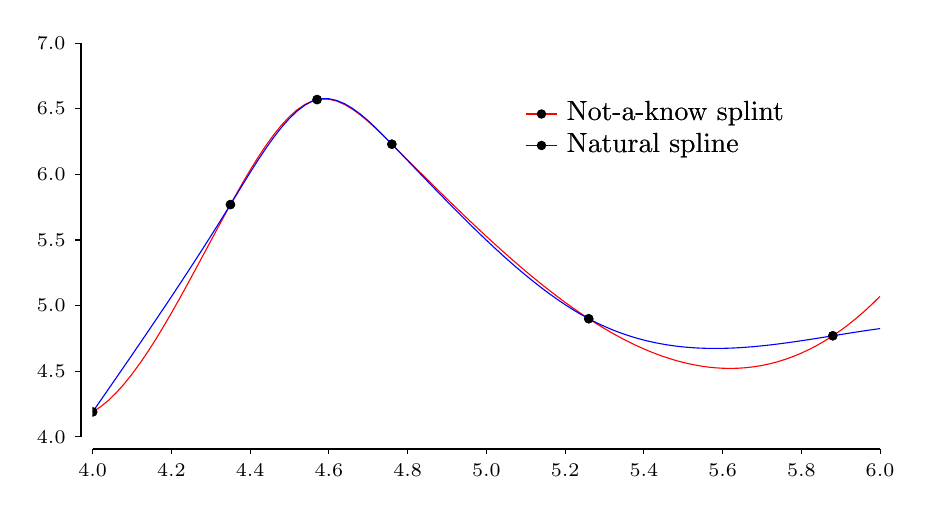
\begin{tikzpicture}[]
\begin{scope}[]
\pgfpathmoveto{ \pgfpointadd{\pgfpointxy {0.0} {0.0}} {\pgfpoint{0cm}{0cm}} }
\pgfpathlineto{ \pgfpointadd{\pgfpointxy {0.0} {0.0}} {\pgfpoint{10cm}{0cm}} }
\pgfpathlineto{ \pgfpointadd{\pgfpointxy {0.0} {0.0}} {\pgfpoint{10cm}{5cm}} }
\pgfpathlineto{ \pgfpointadd{\pgfpointxy {0.0} {0.0}} {\pgfpoint{0cm}{5cm}} }
\pgfpathclose
\pgfusepath{  clip, }
\begin{scope}[shift={(0.0,0.0)}]
\pgfsetxvec{\pgfpoint{5.0cm}{0cm}}
\pgfsetyvec{\pgfpoint{0cm}{1.6666666666666667cm}}
\begin{scope}[shift={(-4.0,-4.0)}]
\begin{scope}[]
\pgfpathmoveto{ \pgfpointadd{\pgfpointxy {4.0} {4.0}} {\pgfpoint{0cm}{0cm}} }
\pgfpathlineto{ \pgfpointadd{\pgfpointxy {4.0} {4.0}} {\pgfpoint{10cm}{0cm}} }
\pgfpathlineto{ \pgfpointadd{\pgfpointxy {4.0} {4.0}} {\pgfpoint{10cm}{5cm}} }
\pgfpathlineto{ \pgfpointadd{\pgfpointxy {4.0} {4.0}} {\pgfpoint{0cm}{5cm}} }
\pgfpathclose
\pgfusepath{  clip, }
\begin{scope}[red]
\pgfpathmoveto{ \pgfpointxy {4.0} {4.19}}
\pgfpathlineto{ \pgfpointxy {4.02} {4.2288933173496535}}
\pgfpathlineto{ \pgfpointxy {4.04} {4.277870024848159}}
\pgfpathlineto{ \pgfpointxy {4.06} {4.336184185327374}}
\pgfpathlineto{ \pgfpointxy {4.08} {4.403089861619165}}
\pgfpathlineto{ \pgfpointxy {4.1} {4.477841116555382}}
\pgfpathlineto{ \pgfpointxy {4.12} {4.559692012967896}}
\pgfpathlineto{ \pgfpointxy {4.14} {4.647896613688557}}
\pgfpathlineto{ \pgfpointxy {4.16} {4.741708981549234}}
\pgfpathlineto{ \pgfpointxy {4.18} {4.84038317938178}}
\pgfpathlineto{ \pgfpointxy {4.2} {4.943173270018062}}
\pgfpathlineto{ \pgfpointxy {4.22} {5.049333316289932}}
\pgfpathlineto{ \pgfpointxy {4.24} {5.158117381029259}}
\pgfpathlineto{ \pgfpointxy {4.26} {5.268779527067894}}
\pgfpathlineto{ \pgfpointxy {4.28} {5.380573817237705}}
\pgfpathlineto{ \pgfpointxy {4.3} {5.492754314370545}}
\pgfpathlineto{ \pgfpointxy {4.32} {5.604575081298282}}
\pgfpathlineto{ \pgfpointxy {4.34} {5.715290180852768}}
\pgfpathlineto{ \pgfpointxy {4.36} {5.824144492927248}}
\pgfpathlineto{ \pgfpointxy {4.38} {5.930171689826624}}
\pgfpathlineto{ \pgfpointxy {4.4} {6.032194236267487}}
\pgfpathlineto{ \pgfpointxy {4.42} {6.129025414027786}}
\pgfpathlineto{ \pgfpointxy {4.44} {6.2194785048854895}}
\pgfpathlineto{ \pgfpointxy {4.46} {6.302366790618549}}
\pgfpathlineto{ \pgfpointxy {4.48} {6.376503553004932}}
\pgfpathlineto{ \pgfpointxy {4.5} {6.440702073822589}}
\pgfpathlineto{ \pgfpointxy {4.52} {6.493775634849485}}
\pgfpathlineto{ \pgfpointxy {4.54} {6.53453751786358}}
\pgfpathlineto{ \pgfpointxy {4.5600000000000005} {6.56180100464283}}
\pgfpathlineto{ \pgfpointxy {4.58} {6.574437556572912}}
\pgfpathlineto{ \pgfpointxy {4.6} {6.572656766016991}}
\pgfpathlineto{ \pgfpointxy {4.62} {6.558006356315717}}
\pgfpathlineto{ \pgfpointxy {4.64} {6.532092230417464}}
\pgfpathlineto{ \pgfpointxy {4.66} {6.496520291270597}}
\pgfpathlineto{ \pgfpointxy {4.68} {6.452896441823487}}
\pgfpathlineto{ \pgfpointxy {4.7} {6.402826585024502}}
\pgfpathlineto{ \pgfpointxy {4.72} {6.347916623822015}}
\pgfpathlineto{ \pgfpointxy {4.74} {6.2897724611643895}}
\pgfpathlineto{ \pgfpointxy {4.76} {6.23}}
\pgfpathlineto{ \pgfpointxy {4.78} {6.169948902792082}}
\pgfpathlineto{ \pgfpointxy {4.8} {6.109943870063351}}
\pgfpathlineto{ \pgfpointxy {4.82} {6.050053361851389}}
\pgfpathlineto{ \pgfpointxy {4.84} {5.990345838193781}}
\pgfpathlineto{ \pgfpointxy {4.86} {5.9308897591281085}}
\pgfpathlineto{ \pgfpointxy {4.88} {5.871753584691959}}
\pgfpathlineto{ \pgfpointxy {4.9} {5.813005774922911}}
\pgfpathlineto{ \pgfpointxy {4.92} {5.754714789858553}}
\pgfpathlineto{ \pgfpointxy {4.94} {5.696949089536464}}
\pgfpathlineto{ \pgfpointxy {4.96} {5.639777133994231}}
\pgfpathlineto{ \pgfpointxy {4.98} {5.583267383269433}}
\pgfpathlineto{ \pgfpointxy {5.0} {5.5274882973996595}}
\pgfpathlineto{ \pgfpointxy {5.02} {5.47250833642249}}
\pgfpathlineto{ \pgfpointxy {5.04} {5.418395960375507}}
\pgfpathlineto{ \pgfpointxy {5.0600000000000005} {5.365219629296296}}
\pgfpathlineto{ \pgfpointxy {5.08} {5.3130478032224415}}
\pgfpathlineto{ \pgfpointxy {5.1} {5.261948942191526}}
\pgfpathlineto{ \pgfpointxy {5.12} {5.21199150624113}}
\pgfpathlineto{ \pgfpointxy {5.140000000000001} {5.1632439554088405}}
\pgfpathlineto{ \pgfpointxy {5.16} {5.115774749732242}}
\pgfpathlineto{ \pgfpointxy {5.18} {5.069652349248916}}
\pgfpathlineto{ \pgfpointxy {5.2} {5.0249452139964434}}
\pgfpathlineto{ \pgfpointxy {5.22} {4.9817218040124125}}
\pgfpathlineto{ \pgfpointxy {5.24} {4.940050579334401}}
\pgfpathlineto{ \pgfpointxy {5.26} {4.9}}
\pgfpathlineto{ \pgfpointxy {5.28} {4.861636317658478}}
\pgfpathlineto{ \pgfpointxy {5.3} {4.8250169504058755}}
\pgfpathlineto{ \pgfpointxy {5.32} {4.790197107949918}}
\pgfpathlineto{ \pgfpointxy {5.34} {4.757231999998338}}
\pgfpathlineto{ \pgfpointxy {5.36} {4.726176836258861}}
\pgfpathlineto{ \pgfpointxy {5.38} {4.697086826439219}}
\pgfpathlineto{ \pgfpointxy {5.4} {4.670017180247137}}
\pgfpathlineto{ \pgfpointxy {5.42} {4.645023107390346}}
\pgfpathlineto{ \pgfpointxy {5.4399999999999995} {4.622159817576572}}
\pgfpathlineto{ \pgfpointxy {5.46} {4.601482520513546}}
\pgfpathlineto{ \pgfpointxy {5.48} {4.583046425908996}}
\pgfpathlineto{ \pgfpointxy {5.5} {4.566906743470651}}
\pgfpathlineto{ \pgfpointxy {5.52} {4.55311868290624}}
\pgfpathlineto{ \pgfpointxy {5.54} {4.5417374539234885}}
\pgfpathlineto{ \pgfpointxy {5.5600000000000005} {4.532818266230128}}
\pgfpathlineto{ \pgfpointxy {5.58} {4.5264163295338875}}
\pgfpathlineto{ \pgfpointxy {5.6} {4.522586853542495}}
\pgfpathlineto{ \pgfpointxy {5.62} {4.521385047963677}}
\pgfpathlineto{ \pgfpointxy {5.640000000000001} {4.522866122505165}}
\pgfpathlineto{ \pgfpointxy {5.66} {4.527085286874686}}
\pgfpathlineto{ \pgfpointxy {5.68} {4.534097750779969}}
\pgfpathlineto{ \pgfpointxy {5.7} {4.543958723928742}}
\pgfpathlineto{ \pgfpointxy {5.72} {4.556723416028735}}
\pgfpathlineto{ \pgfpointxy {5.74} {4.572447036787675}}
\pgfpathlineto{ \pgfpointxy {5.76} {4.591184795913292}}
\pgfpathlineto{ \pgfpointxy {5.78} {4.612991903113314}}
\pgfpathlineto{ \pgfpointxy {5.8} {4.637923568095469}}
\pgfpathlineto{ \pgfpointxy {5.82} {4.666035000567487}}
\pgfpathlineto{ \pgfpointxy {5.84} {4.697381410237095}}
\pgfpathlineto{ \pgfpointxy {5.86} {4.732018006812025}}
\pgfpathlineto{ \pgfpointxy {5.88} {4.77}}
\pgfpathlineto{ \pgfpointxy {5.9} {4.811382599508753}}
\pgfpathlineto{ \pgfpointxy {5.92} {4.85622101504601}}
\pgfpathlineto{ \pgfpointxy {5.9399999999999995} {4.904570456319501}}
\pgfpathlineto{ \pgfpointxy {5.96} {4.9564861330369565}}
\pgfpathlineto{ \pgfpointxy {5.98} {5.0120232549061035}}
\pgfpathlineto{ \pgfpointxy {6.0} {5.071237031634667}}
\pgfusepath{ stroke, }
\end{scope}
\end{scope}
\begin{scope}[]
\pgfpathmoveto{ \pgfpointadd{\pgfpointxy {4.0} {4.0}} {\pgfpoint{0cm}{0cm}} }
\pgfpathlineto{ \pgfpointadd{\pgfpointxy {4.0} {4.0}} {\pgfpoint{10cm}{0cm}} }
\pgfpathlineto{ \pgfpointadd{\pgfpointxy {4.0} {4.0}} {\pgfpoint{10cm}{5cm}} }
\pgfpathlineto{ \pgfpointadd{\pgfpointxy {4.0} {4.0}} {\pgfpoint{0cm}{5cm}} }
\pgfpathclose
\pgfusepath{  clip, }
\node at (4.0,4.19) [fill=black,draw=black,circle,inner sep=0.0pt,minimum width =3.0pt,minimum height=3.0pt] {};
\node at (4.35,5.77) [fill=black,draw=black,circle,inner sep=0.0pt,minimum width =3.0pt,minimum height=3.0pt] {};
\node at (4.57,6.57) [fill=black,draw=black,circle,inner sep=0.0pt,minimum width =3.0pt,minimum height=3.0pt] {};
\node at (4.76,6.23) [fill=black,draw=black,circle,inner sep=0.0pt,minimum width =3.0pt,minimum height=3.0pt] {};
\node at (5.26,4.9) [fill=black,draw=black,circle,inner sep=0.0pt,minimum width =3.0pt,minimum height=3.0pt] {};
\node at (5.88,4.77) [fill=black,draw=black,circle,inner sep=0.0pt,minimum width =3.0pt,minimum height=3.0pt] {};
\end{scope}
\end{scope}
\end{scope}
\pgfsetxvec{\pgfpoint{1cm}{0cm}}
\pgfsetyvec{\pgfpoint{0cm}{1cm}}
\end{scope}
\draw[red] (5.5,4.1) -- (5.9,4.1);
\draw[opacity=0.0,white] (5.5,4.2) -- (5.5,4.0);
\node at (5.9,4.1) [right,] {Not-a-know splint};
\node at (5.7,4.1) [fill=black,draw=black,circle,inner sep=0.0pt,minimum width =3.0pt,minimum height=3.0pt] {};
\node at (5.9,4.1) [right,] {Not-a-know splint};
\begin{scope}[]
\pgfpathmoveto{ \pgfpointadd{\pgfpointxy {0.0} {0.0}} {\pgfpoint{0cm}{0cm}} }
\pgfpathlineto{ \pgfpointadd{\pgfpointxy {0.0} {0.0}} {\pgfpoint{10cm}{0cm}} }
\pgfpathlineto{ \pgfpointadd{\pgfpointxy {0.0} {0.0}} {\pgfpoint{10cm}{5cm}} }
\pgfpathlineto{ \pgfpointadd{\pgfpointxy {0.0} {0.0}} {\pgfpoint{0cm}{5cm}} }
\pgfpathclose
\pgfusepath{  clip, }
\begin{scope}[shift={(0.0,0.0)}]
\pgfsetxvec{\pgfpoint{5.0cm}{0cm}}
\pgfsetyvec{\pgfpoint{0cm}{1.6666666666666667cm}}
\begin{scope}[shift={(-4.0,-4.0)}]
\begin{scope}[]
\pgfpathmoveto{ \pgfpointadd{\pgfpointxy {4.0} {4.0}} {\pgfpoint{0cm}{0cm}} }
\pgfpathlineto{ \pgfpointadd{\pgfpointxy {4.0} {4.0}} {\pgfpoint{10cm}{0cm}} }
\pgfpathlineto{ \pgfpointadd{\pgfpointxy {4.0} {4.0}} {\pgfpoint{10cm}{5cm}} }
\pgfpathlineto{ \pgfpointadd{\pgfpointxy {4.0} {4.0}} {\pgfpoint{0cm}{5cm}} }
\pgfpathclose
\pgfusepath{  clip, }
\begin{scope}[blue]
\pgfpathmoveto{ \pgfpointxy {4.0} {4.19}}
\pgfpathlineto{ \pgfpointxy {4.02} {4.27659219042123}}
\pgfpathlineto{ \pgfpointxy {4.04} {4.363256980820145}}
\pgfpathlineto{ \pgfpointxy {4.06} {4.450066971174415}}
\pgfpathlineto{ \pgfpointxy {4.08} {4.537094761461732}}
\pgfpathlineto{ \pgfpointxy {4.1} {4.624412951659764}}
\pgfpathlineto{ \pgfpointxy {4.12} {4.712094141746202}}
\pgfpathlineto{ \pgfpointxy {4.14} {4.800210931698716}}
\pgfpathlineto{ \pgfpointxy {4.16} {4.888835921494997}}
\pgfpathlineto{ \pgfpointxy {4.18} {4.978041711112716}}
\pgfpathlineto{ \pgfpointxy {4.2} {5.067900900529561}}
\pgfpathlineto{ \pgfpointxy {4.22} {5.158486089723204}}
\pgfpathlineto{ \pgfpointxy {4.24} {5.249869878671334}}
\pgfpathlineto{ \pgfpointxy {4.26} {5.342124867351624}}
\pgfpathlineto{ \pgfpointxy {4.28} {5.43532365574176}}
\pgfpathlineto{ \pgfpointxy {4.3} {5.529538843819415}}
\pgfpathlineto{ \pgfpointxy {4.32} {5.624843031562279}}
\pgfpathlineto{ \pgfpointxy {4.34} {5.721308818948022}}
\pgfpathlineto{ \pgfpointxy {4.36} {5.818974279573464}}
\pgfpathlineto{ \pgfpointxy {4.38} {5.917083380275411}}
\pgfpathlineto{ \pgfpointxy {4.4} {6.014085981130691}}
\pgfpathlineto{ \pgfpointxy {4.42} {6.108397415835243}}
\pgfpathlineto{ \pgfpointxy {4.44} {6.198433018085027}}
\pgfpathlineto{ \pgfpointxy {4.46} {6.282608121575982}}
\pgfpathlineto{ \pgfpointxy {4.48} {6.359338060004066}}
\pgfpathlineto{ \pgfpointxy {4.5} {6.427038167065223}}
\pgfpathlineto{ \pgfpointxy {4.52} {6.484123776455401}}
\pgfpathlineto{ \pgfpointxy {4.54} {6.529010221870556}}
\pgfpathlineto{ \pgfpointxy {4.5600000000000005} {6.560112837006632}}
\pgfpathlineto{ \pgfpointxy {4.58} {6.575914836921859}}
\pgfpathlineto{ \pgfpointxy {4.6} {6.576460708006886}}
\pgfpathlineto{ \pgfpointxy {4.62} {6.563356207984786}}
\pgfpathlineto{ \pgfpointxy {4.64} {6.538274975940911}}
\pgfpathlineto{ \pgfpointxy {4.66} {6.502890650960607}}
\pgfpathlineto{ \pgfpointxy {4.68} {6.458876872129232}}
\pgfpathlineto{ \pgfpointxy {4.7} {6.4079072785321305}}
\pgfpathlineto{ \pgfpointxy {4.72} {6.351655509254659}}
\pgfpathlineto{ \pgfpointxy {4.74} {6.291795203382164}}
\pgfpathlineto{ \pgfpointxy {4.76} {6.23}}
\pgfpathlineto{ \pgfpointxy {4.78} {6.16768423115035}}
\pgfpathlineto{ \pgfpointxy {4.8} {6.105225000702742}}
\pgfpathlineto{ \pgfpointxy {4.82} {6.042740105483533}}
\pgfpathlineto{ \pgfpointxy {4.84} {5.98034734231909}}
\pgfpathlineto{ \pgfpointxy {4.86} {5.9181645080357645}}
\pgfpathlineto{ \pgfpointxy {4.88} {5.856309399459924}}
\pgfpathlineto{ \pgfpointxy {4.9} {5.794899813417925}}
\pgfpathlineto{ \pgfpointxy {4.92} {5.734053546736131}}
\pgfpathlineto{ \pgfpointxy {4.94} {5.6738883962408995}}
\pgfpathlineto{ \pgfpointxy {4.96} {5.614522158758593}}
\pgfpathlineto{ \pgfpointxy {4.98} {5.556072631115571}}
\pgfpathlineto{ \pgfpointxy {5.0} {5.498657610138196}}
\pgfpathlineto{ \pgfpointxy {5.02} {5.442394892652826}}
\pgfpathlineto{ \pgfpointxy {5.04} {5.387402275485819}}
\pgfpathlineto{ \pgfpointxy {5.0600000000000005} {5.333797555463539}}
\pgfpathlineto{ \pgfpointxy {5.08} {5.281698529412348}}
\pgfpathlineto{ \pgfpointxy {5.1} {5.231222994158605}}
\pgfpathlineto{ \pgfpointxy {5.12} {5.182488746528666}}
\pgfpathlineto{ \pgfpointxy {5.140000000000001} {5.1356135833488965}}
\pgfpathlineto{ \pgfpointxy {5.16} {5.090715301445657}}
\pgfpathlineto{ \pgfpointxy {5.18} {5.047911697645307}}
\pgfpathlineto{ \pgfpointxy {5.2} {5.007320568774205}}
\pgfpathlineto{ \pgfpointxy {5.22} {4.969059711658713}}
\pgfpathlineto{ \pgfpointxy {5.24} {4.93324692312519}}
\pgfpathlineto{ \pgfpointxy {5.26} {4.9}}
\pgfpathlineto{ \pgfpointxy {5.28} {4.869402678013522}}
\pgfpathlineto{ \pgfpointxy {5.3} {4.8414024485122304}}
\pgfpathlineto{ \pgfpointxy {5.32} {4.815912741746616}}
\pgfpathlineto{ \pgfpointxy {5.34} {4.792846987967176}}
\pgfpathlineto{ \pgfpointxy {5.36} {4.7721186174244}}
\pgfpathlineto{ \pgfpointxy {5.38} {4.753641060368786}}
\pgfpathlineto{ \pgfpointxy {5.4} {4.737327747050826}}
\pgfpathlineto{ \pgfpointxy {5.42} {4.723092107721014}}
\pgfpathlineto{ \pgfpointxy {5.4399999999999995} {4.710847572629844}}
\pgfpathlineto{ \pgfpointxy {5.46} {4.700507572027809}}
\pgfpathlineto{ \pgfpointxy {5.48} {4.691985536165404}}
\pgfpathlineto{ \pgfpointxy {5.5} {4.685194895293122}}
\pgfpathlineto{ \pgfpointxy {5.52} {4.680049079661458}}
\pgfpathlineto{ \pgfpointxy {5.54} {4.676461519520904}}
\pgfpathlineto{ \pgfpointxy {5.5600000000000005} {4.674345645121956}}
\pgfpathlineto{ \pgfpointxy {5.58} {4.6736148867151055}}
\pgfpathlineto{ \pgfpointxy {5.6} {4.674182674550848}}
\pgfpathlineto{ \pgfpointxy {5.62} {4.675962438879676}}
\pgfpathlineto{ \pgfpointxy {5.640000000000001} {4.678867609952086}}
\pgfpathlineto{ \pgfpointxy {5.66} {4.682811618018568}}
\pgfpathlineto{ \pgfpointxy {5.68} {4.687707893329618}}
\pgfpathlineto{ \pgfpointxy {5.7} {4.693469866135731}}
\pgfpathlineto{ \pgfpointxy {5.72} {4.700010966687398}}
\pgfpathlineto{ \pgfpointxy {5.74} {4.707244625235115}}
\pgfpathlineto{ \pgfpointxy {5.76} {4.715084272029376}}
\pgfpathlineto{ \pgfpointxy {5.78} {4.723443337320674}}
\pgfpathlineto{ \pgfpointxy {5.8} {4.732235251359502}}
\pgfpathlineto{ \pgfpointxy {5.82} {4.741373444396355}}
\pgfpathlineto{ \pgfpointxy {5.84} {4.750771346681726}}
\pgfpathlineto{ \pgfpointxy {5.86} {4.7603423884661105}}
\pgfpathlineto{ \pgfpointxy {5.88} {4.77}}
\pgfpathlineto{ \pgfpointxy {5.9} {4.77965761153389}}
\pgfpathlineto{ \pgfpointxy {5.92} {4.789228653318274}}
\pgfpathlineto{ \pgfpointxy {5.9399999999999995} {4.7986265556036445}}
\pgfpathlineto{ \pgfpointxy {5.96} {4.807764748640497}}
\pgfpathlineto{ \pgfpointxy {5.98} {4.816556662679326}}
\pgfpathlineto{ \pgfpointxy {6.0} {4.824915727970623}}
\pgfusepath{ stroke, }
\end{scope}
\end{scope}
\begin{scope}[]
\pgfpathmoveto{ \pgfpointadd{\pgfpointxy {4.0} {4.0}} {\pgfpoint{0cm}{0cm}} }
\pgfpathlineto{ \pgfpointadd{\pgfpointxy {4.0} {4.0}} {\pgfpoint{10cm}{0cm}} }
\pgfpathlineto{ \pgfpointadd{\pgfpointxy {4.0} {4.0}} {\pgfpoint{10cm}{5cm}} }
\pgfpathlineto{ \pgfpointadd{\pgfpointxy {4.0} {4.0}} {\pgfpoint{0cm}{5cm}} }
\pgfpathclose
\pgfusepath{  clip, }
\node at (4.0,4.19) [fill=black,draw=black,circle,inner sep=0.0pt,minimum width =3.0pt,minimum height=3.0pt] {};
\node at (4.35,5.77) [fill=black,draw=black,circle,inner sep=0.0pt,minimum width =3.0pt,minimum height=3.0pt] {};
\node at (4.57,6.57) [fill=black,draw=black,circle,inner sep=0.0pt,minimum width =3.0pt,minimum height=3.0pt] {};
\node at (4.76,6.23) [fill=black,draw=black,circle,inner sep=0.0pt,minimum width =3.0pt,minimum height=3.0pt] {};
\node at (5.26,4.9) [fill=black,draw=black,circle,inner sep=0.0pt,minimum width =3.0pt,minimum height=3.0pt] {};
\node at (5.88,4.77) [fill=black,draw=black,circle,inner sep=0.0pt,minimum width =3.0pt,minimum height=3.0pt] {};
\end{scope}
\end{scope}
\end{scope}
\pgfsetxvec{\pgfpoint{1cm}{0cm}}
\pgfsetyvec{\pgfpoint{0cm}{1cm}}
\end{scope}
\draw[blue] (5.5,3.7) -- (5.9,3.7);
\draw[opacity=0.0,white] (5.5,3.8000000000000003) -- (5.5,3.6);
\node at (5.9,3.7) [right,] {Natural spline};
\node at (5.7,3.7) [fill=black,draw=black,circle,inner sep=0.0pt,minimum width =3.0pt,minimum height=3.0pt] {};
\node at (5.9,3.7) [right,] {Natural spline};
\begin{scope}[shift={(0.0,0.0)}]
\pgfsetxvec{\pgfpoint{5.0cm}{0cm}}
\pgfsetyvec{\pgfpoint{0cm}{1.6666666666666667cm}}
\begin{scope}[shift={(-4.0,-4.0)}]
\begin{scope}[thick,black,fill=white]
\pgfpathmoveto{ \pgfpointadd{\pgfpointxy {4.0} {4.0}} {\pgfpoint{0}{-0.15cm}} }
\pgfpathlineto{ \pgfpointadd{\pgfpointxy {6.0} {4.0}} {\pgfpoint{0}{-0.15cm}} }
\pgfpathmoveto{ \pgfpointadd{\pgfpointxy {4.0} {4.0}} {\pgfpoint{-0.15cm}{0}} }
\pgfpathlineto{ \pgfpointadd{\pgfpointxy {4.0} {7.0}} {\pgfpoint{-0.15cm}{0}} }
\pgfusepath{ stroke, }
\end{scope}
\begin{scope}[yshift=-0.15cm]
\draw[] [shift={(4.0,4.0)}] (0,0) -- (0,-2pt) node[below]{ \scriptsize{\num[round-mode=places,round-precision=1]{4.0}}};
\draw[] [shift={(4.2,4.0)}] (0,0) -- (0,-2pt) node[below]{ \scriptsize{\num[round-mode=places,round-precision=1]{4.2}}};
\draw[] [shift={(4.4,4.0)}] (0,0) -- (0,-2pt) node[below]{ \scriptsize{\num[round-mode=places,round-precision=1]{4.4}}};
\draw[] [shift={(4.6,4.0)}] (0,0) -- (0,-2pt) node[below]{ \scriptsize{\num[round-mode=places,round-precision=1]{4.6}}};
\draw[] [shift={(4.8,4.0)}] (0,0) -- (0,-2pt) node[below]{ \scriptsize{\num[round-mode=places,round-precision=1]{4.8}}};
\draw[] [shift={(5.0,4.0)}] (0,0) -- (0,-2pt) node[below]{ \scriptsize{\num[round-mode=places,round-precision=1]{5.0}}};
\draw[] [shift={(5.2,4.0)}] (0,0) -- (0,-2pt) node[below]{ \scriptsize{\num[round-mode=places,round-precision=1]{5.2}}};
\draw[] [shift={(5.4,4.0)}] (0,0) -- (0,-2pt) node[below]{ \scriptsize{\num[round-mode=places,round-precision=1]{5.4}}};
\draw[] [shift={(5.6,4.0)}] (0,0) -- (0,-2pt) node[below]{ \scriptsize{\num[round-mode=places,round-precision=1]{5.6}}};
\draw[] [shift={(5.8,4.0)}] (0,0) -- (0,-2pt) node[below]{ \scriptsize{\num[round-mode=places,round-precision=1]{5.8}}};
\draw[] [shift={(6.0,4.0)}] (0,0) -- (0,-2pt) node[below]{ \scriptsize{\num[round-mode=places,round-precision=1]{6.0}}};
\end{scope}
\begin{scope}[xshift=-0.15cm]
\draw[] [shift={(4.0,4.0)}] (0,0) -- (-2pt,0) node[left]{ \scriptsize{\num[round-mode=places,round-precision=1]{4.0}}};
\draw[] [shift={(4.0,4.5)}] (0,0) -- (-2pt,0) node[left]{ \scriptsize{\num[round-mode=places,round-precision=1]{4.5}}};
\draw[] [shift={(4.0,5.0)}] (0,0) -- (-2pt,0) node[left]{ \scriptsize{\num[round-mode=places,round-precision=1]{5.0}}};
\draw[] [shift={(4.0,5.5)}] (0,0) -- (-2pt,0) node[left]{ \scriptsize{\num[round-mode=places,round-precision=1]{5.5}}};
\draw[] [shift={(4.0,6.0)}] (0,0) -- (-2pt,0) node[left]{ \scriptsize{\num[round-mode=places,round-precision=1]{6.0}}};
\draw[] [shift={(4.0,6.5)}] (0,0) -- (-2pt,0) node[left]{ \scriptsize{\num[round-mode=places,round-precision=1]{6.5}}};
\draw[] [shift={(4.0,7.0)}] (0,0) -- (-2pt,0) node[left]{ \scriptsize{\num[round-mode=places,round-precision=1]{7.0}}};
\end{scope}
\end{scope}
\end{scope}
\pgfsetxvec{\pgfpoint{1cm}{0cm}}
\pgfsetyvec{\pgfpoint{0cm}{1cm}}
\end{tikzpicture}
\end{document}

\captionsetup{singlelinecheck=off}
\caption[asdf]{Cubic splines, with different end point conditions.}
\end{figure}
\section{Sub figures}


The with-sub-figure macro makes it possible to draw with a new set of transformations
within the same tikz figure. In addition to the with-tikz-to-stream arguments, the sub-figure also
expects the offset from (0,0) in the default cm frame.

\begin{figure}[H]
\centering
\documentclass{standalone}
\ifx\HCode\UnDef\else\def\pgfsysdriver{pgfsys-tex4ht.def}\fi
\usepackage[usenames,dvipsnames,svgnames,table]{xcolor}
\usepackage{tikz}
\usepackage{color}
\usepackage{siunitx}
\usetikzlibrary{arrows,shapes}
\begin{document}
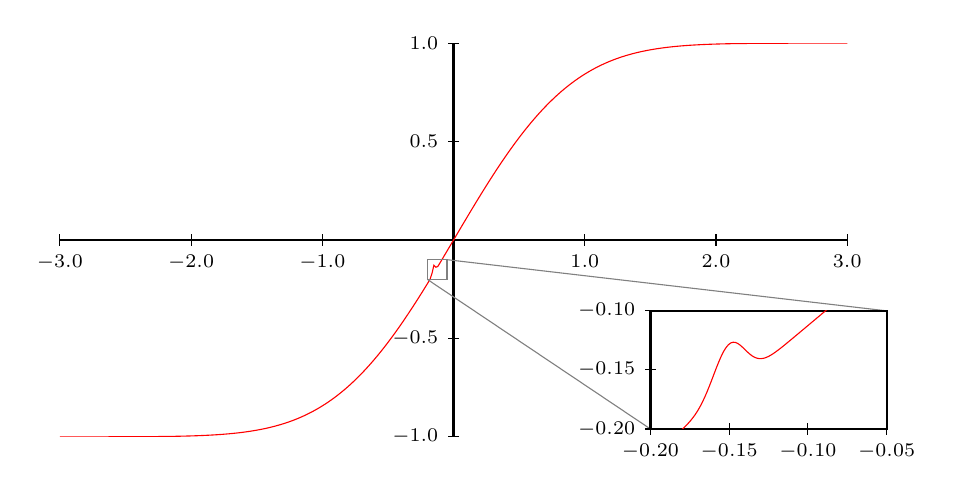
\begin{tikzpicture}
\begin{scope}[shift={(0.0,0.0)}]
\pgfsetxvec{\pgfpoint{1.6666666cm}{0cm}}
\pgfsetyvec{\pgfpoint{0cm}{2.5cm}}
\begin{scope}[shift={(3.0,1.0)}]
\begin{scope}[thick,black,fill=white]
\pgfpathmoveto{ \pgfpointxy {-3.0} {0.0}}
\pgfpathlineto{ \pgfpointxy {3.0} {0.0}}
\pgfpathmoveto{ \pgfpointxy {0.0} {-1.0}}
\pgfpathlineto{ \pgfpointxy {0.0} {1.0}}
\pgfusepath{ stroke, }
\end{scope}
\begin{scope}[yshift=2.5cm]
\draw[] [shift={(-3.0,-1.0)}] (0,2pt) -- (0,-2pt) node[below]{ \scriptsize{\num[round-mode=places,round-precision=1]{-3.0}}};
\draw[] [shift={(-2.0,-1.0)}] (0,2pt) -- (0,-2pt) node[below]{ \scriptsize{\num[round-mode=places,round-precision=1]{-2.0}}};
\draw[] [shift={(-1.0,-1.0)}] (0,2pt) -- (0,-2pt) node[below]{ \scriptsize{\num[round-mode=places,round-precision=1]{-1.0}}};
\draw[] [shift={(1.0,-1.0)}] (0,2pt) -- (0,-2pt) node[below]{ \scriptsize{\num[round-mode=places,round-precision=1]{1.0}}};
\draw[] [shift={(2.0,-1.0)}] (0,2pt) -- (0,-2pt) node[below]{ \scriptsize{\num[round-mode=places,round-precision=1]{2.0}}};
\draw[] [shift={(3.0,-1.0)}] (0,2pt) -- (0,-2pt) node[below]{ \scriptsize{\num[round-mode=places,round-precision=1]{3.0}}};
\end{scope}
\begin{scope}[xshift=5.0cm]
\draw[] [shift={(-3.0,-1.0)}] (2pt,0) -- (-2pt,0) node[left]{ \scriptsize{\num[round-mode=places,round-precision=1]{-1.0}}};
\draw[] [shift={(-3.0,-0.5)}] (2pt,0) -- (-2pt,0) node[left]{ \scriptsize{\num[round-mode=places,round-precision=1]{-0.5}}};
\draw[] [shift={(-3.0,0.5)}] (2pt,0) -- (-2pt,0) node[left]{ \scriptsize{\num[round-mode=places,round-precision=1]{0.5}}};
\draw[] [shift={(-3.0,1.0)}] (2pt,0) -- (-2pt,0) node[left]{ \scriptsize{\num[round-mode=places,round-precision=1]{1.0}}};
\end{scope}
\end{scope}
\pgfsetxvec{\pgfpoint{1cm}{0cm}}
\pgfsetyvec{\pgfpoint{0cm}{1cm}}
\end{scope}
\begin{scope}[]
\pgfpointadd{\pgfpointxy {0.0} {0.0}} {\pgfpoint{0cm}{0cm}}\pgfpathmoveto{ NIL }
\pgfpointadd{\pgfpointxy {0.0} {0.0}} {\pgfpoint{10cm}{0cm}}\pgfpathlineto{ NIL }
\pgfpointadd{\pgfpointxy {0.0} {0.0}} {\pgfpoint{10cm}{5cm}}\pgfpathlineto{ NIL }
\pgfpointadd{\pgfpointxy {0.0} {0.0}} {\pgfpoint{0cm}{5cm}}\pgfpathlineto{ NIL }
\pgfpathclose
\pgfusepath{  clip, }
\begin{scope}[shift={(0.0,0.0)}]
\pgfsetxvec{\pgfpoint{1.6666666cm}{0cm}}
\pgfsetyvec{\pgfpoint{0cm}{2.5cm}}
\begin{scope}[shift={(3.0,1.0)}]
\begin{scope}[red]
\pgfpathmoveto{ \pgfpointxy {-3.0} {-0.9999778948512584}}
\pgfpathlineto{ \pgfpointxy {-2.985} {-0.9999757083350379}}
\pgfpathlineto{ \pgfpointxy {-2.97} {-0.9999733170663182}}
\pgfpathlineto{ \pgfpointxy {-2.955} {-0.9999707029673122}}
\pgfpathlineto{ \pgfpointxy {-2.94} {-0.99996784664559}}
\pgfpathlineto{ \pgfpointxy {-2.925} {-0.9999647269538418}}
\pgfpathlineto{ \pgfpointxy {-2.91} {-0.9999613212537493}}
\pgfpathlineto{ \pgfpointxy {-2.895} {-0.9999576048834065}}
\pgfpathlineto{ \pgfpointxy {-2.88} {-0.9999535514455115}}
\pgfpathlineto{ \pgfpointxy {-2.865} {-0.9999491322368748}}
\pgfpathlineto{ \pgfpointxy {-2.85} {-0.9999443164424575}}
\pgfpathlineto{ \pgfpointxy {-2.835} {-0.9999390709691429}}
\pgfpathlineto{ \pgfpointxy {-2.82} {-0.9999333598509589}}
\pgfpathlineto{ \pgfpointxy {-2.805} {-0.9999271447394446}}
\pgfpathlineto{ \pgfpointxy {-2.79} {-0.9999203839664113}}
\pgfpathlineto{ \pgfpointxy {-2.775} {-0.9999130332073615}}
\pgfpathlineto{ \pgfpointxy {-2.76} {-0.9999050442982494}}
\pgfpathlineto{ \pgfpointxy {-2.745} {-0.9998963658439115}}
\pgfpathlineto{ \pgfpointxy {-2.73} {-0.9998869427777993}}
\pgfpathlineto{ \pgfpointxy {-2.715} {-0.9998767154431919}}
\pgfpathlineto{ \pgfpointxy {-2.7} {-0.999865620549059}}
\pgfpathlineto{ \pgfpointxy {-2.685} {-0.999853589536517}}
\pgfpathlineto{ \pgfpointxy {-2.67} {-0.9998405496871464}}
\pgfpathlineto{ \pgfpointxy {-2.655} {-0.9998264223308793}}
\pgfpathlineto{ \pgfpointxy {-2.64} {-0.9998111241177303}}
\pgfpathlineto{ \pgfpointxy {-2.625} {-0.9997945649944869}}
\pgfpathlineto{ \pgfpointxy {-2.6100001} {-0.9997766495590875}}
\pgfpathlineto{ \pgfpointxy {-2.595} {-0.9997572748749847}}
\pgfpathlineto{ \pgfpointxy {-2.58} {-0.9997363318915964}}
\pgfpathlineto{ \pgfpointxy {-2.565} {-0.9997137040964125}}
\pgfpathlineto{ \pgfpointxy {-2.55} {-0.9996892661202884}}
\pgfpathlineto{ \pgfpointxy {-2.535} {-0.9996628860762126}}
\pgfpathlineto{ \pgfpointxy {-2.52} {-0.9996344214396051}}
\pgfpathlineto{ \pgfpointxy {-2.505} {-0.9996037221103481}}
\pgfpathlineto{ \pgfpointxy {-2.49} {-0.9995706266688278}}
\pgfpathlineto{ \pgfpointxy {-2.475} {-0.9995349645820102}}
\pgfpathlineto{ \pgfpointxy {-2.46} {-0.9994965548342742}}
\pgfpathlineto{ \pgfpointxy {-2.445} {-0.9994552028377658}}
\pgfpathlineto{ \pgfpointxy {-2.43} {-0.9994107046969803}}
\pgfpathlineto{ \pgfpointxy {-2.415} {-0.9993628411831741}}
\pgfpathlineto{ \pgfpointxy {-2.4} {-0.9993113823951093}}
\pgfpathlineto{ \pgfpointxy {-2.385} {-0.9992560815728813}}
\pgfpathlineto{ \pgfpointxy {-2.37} {-0.9991966793596809}}
\pgfpathlineto{ \pgfpointxy {-2.355} {-0.9991329013480114}}
\pgfpathlineto{ \pgfpointxy {-2.3400002} {-0.9990644548790096}}
\pgfpathlineto{ \pgfpointxy {-2.325} {-0.9989910302783986}}
\pgfpathlineto{ \pgfpointxy {-2.31} {-0.9989123017378415}}
\pgfpathlineto{ \pgfpointxy {-2.295} {-0.9988279258631217}}
\pgfpathlineto{ \pgfpointxy {-2.28} {-0.9987375351241278}}
\pgfpathlineto{ \pgfpointxy {-2.265} {-0.9986407474173038}}
\pgfpathlineto{ \pgfpointxy {-2.25} {-0.99853715350349}}
\pgfpathlineto{ \pgfpointxy {-2.2350001} {-0.9984263272279732}}
\pgfpathlineto{ \pgfpointxy {-2.22} {-0.9983078149049633}}
\pgfpathlineto{ \pgfpointxy {-2.205} {-0.9981811409848902}}
\pgfpathlineto{ \pgfpointxy {-2.19} {-0.9980458074115153}}
\pgfpathlineto{ \pgfpointxy {-2.175} {-0.9979012818975463}}
\pgfpathlineto{ \pgfpointxy {-2.16} {-0.9977470154175949}}
\pgfpathlineto{ \pgfpointxy {-2.145} {-0.9975824189686803}}
\pgfpathlineto{ \pgfpointxy {-2.13} {-0.9974068859107228}}
\pgfpathlineto{ \pgfpointxy {-2.115} {-0.9972197680997329}}
\pgfpathlineto{ \pgfpointxy {-2.1} {-0.9970203940990304}}
\pgfpathlineto{ \pgfpointxy {-2.085} {-0.996808059480499}}
\pgfpathlineto{ \pgfpointxy {-2.07} {-0.9965820153161545}}
\pgfpathlineto{ \pgfpointxy {-2.055} {-0.9963414947033638}}
\pgfpathlineto{ \pgfpointxy {-2.04} {-0.9960856759455314}}
\pgfpathlineto{ \pgfpointxy {-2.025} {-0.9958137174811054}}
\pgfpathlineto{ \pgfpointxy {-2.01} {-0.995524721420797}}
\pgfpathlineto{ \pgfpointxy {-1.995} {-0.9952177656037218}}
\pgfpathlineto{ \pgfpointxy {-1.98} {-0.99489187942463}}
\pgfpathlineto{ \pgfpointxy {-1.965} {-0.994546050431862}}
\pgfpathlineto{ \pgfpointxy {-1.95} {-0.9941792216068389}}
\pgfpathlineto{ \pgfpointxy {-1.9350001} {-0.9937902946014261}}
\pgfpathlineto{ \pgfpointxy {-1.9200001} {-0.9933781233472766}}
\pgfpathlineto{ \pgfpointxy {-1.905} {-0.9929415139895813}}
\pgfpathlineto{ \pgfpointxy {-1.89} {-0.9924792268868523}}
\pgfpathlineto{ \pgfpointxy {-1.875} {-0.9919899723248453}}
\pgfpathlineto{ \pgfpointxy {-1.86} {-0.9914724099175326}}
\pgfpathlineto{ \pgfpointxy {-1.845} {-0.9909251512583926}}
\pgfpathlineto{ \pgfpointxy {-1.83} {-0.9903467440356116}}
\pgfpathlineto{ \pgfpointxy {-1.815} {-0.989735694565581}}
\pgfpathlineto{ \pgfpointxy {-1.8000001} {-0.9890904549939443}}
\pgfpathlineto{ \pgfpointxy {-1.7850001} {-0.9884094183935574}}
\pgfpathlineto{ \pgfpointxy {-1.77} {-0.9876909094700103}}
\pgfpathlineto{ \pgfpointxy {-1.755} {-0.9869332261163117}}
\pgfpathlineto{ \pgfpointxy {-1.74} {-0.9861345820588053}}
\pgfpathlineto{ \pgfpointxy {-1.725} {-0.9852931457556806}}
\pgfpathlineto{ \pgfpointxy {-1.71} {-0.9844070163473294}}
\pgfpathlineto{ \pgfpointxy {-1.695} {-0.983474242634905}}
\pgfpathlineto{ \pgfpointxy {-1.6800001} {-0.9824928178594202}}
\pgfpathlineto{ \pgfpointxy {-1.6650001} {-0.9814606593383027}}
\pgfpathlineto{ \pgfpointxy {-1.65} {-0.9803756258274028}}
\pgfpathlineto{ \pgfpointxy {-1.635} {-0.9792355416260458}}
\pgfpathlineto{ \pgfpointxy {-1.62} {-0.9780381505422548}}
\pgfpathlineto{ \pgfpointxy {-1.605} {-0.9767811255765453}}
\pgfpathlineto{ \pgfpointxy {-1.59} {-0.9754620987836773}}
\pgfpathlineto{ \pgfpointxy {-1.575} {-0.974078621731563}}
\pgfpathlineto{ \pgfpointxy {-1.5600001} {-0.972628222882936}}
\pgfpathlineto{ \pgfpointxy {-1.5450001} {-0.9711083262499621}}
\pgfpathlineto{ \pgfpointxy {-1.5300001} {-0.9695163254808733}}
\pgfpathlineto{ \pgfpointxy {-1.515} {-0.967849535554207}}
\pgfpathlineto{ \pgfpointxy {-1.5} {-0.9661052690277371}}
\pgfpathlineto{ \pgfpointxy {-1.485} {-0.9642807155660278}}
\pgfpathlineto{ \pgfpointxy {-1.47} {-0.9623730304958918}}
\pgfpathlineto{ \pgfpointxy {-1.455} {-0.9603793399364072}}
\pgfpathlineto{ \pgfpointxy {-1.44} {-0.9582967104453198}}
\pgfpathlineto{ \pgfpointxy {-1.4250001} {-0.9561221356984225}}
\pgfpathlineto{ \pgfpointxy {-1.4100001} {-0.9538525887297505}}
\pgfpathlineto{ \pgfpointxy {-1.395} {-0.9514849669948426}}
\pgfpathlineto{ \pgfpointxy {-1.38} {-0.9490161689966897}}
\pgfpathlineto{ \pgfpointxy {-1.365} {-0.9464430359161858}}
\pgfpathlineto{ \pgfpointxy {-1.35} {-0.9437623278867372}}
\pgfpathlineto{ \pgfpointxy {-1.335} {-0.9409708392198176}}
\pgfpathlineto{ \pgfpointxy {-1.32} {-0.9380652828235414}}
\pgfpathlineto{ \pgfpointxy {-1.3050001} {-0.9350423680815523}}
\pgfpathlineto{ \pgfpointxy {-1.2900001} {-0.9318987712886478}}
\pgfpathlineto{ \pgfpointxy {-1.2750001} {-0.9286311283734742}}
\pgfpathlineto{ \pgfpointxy {-1.26} {-0.9252360326788243}}
\pgfpathlineto{ \pgfpointxy {-1.245} {-0.9217101983808839}}
\pgfpathlineto{ \pgfpointxy {-1.23} {-0.9180501849922466}}
\pgfpathlineto{ \pgfpointxy {-1.215} {-0.914252606844666}}
\pgfpathlineto{ \pgfpointxy {-1.2} {-0.9103140543342333}}
\pgfpathlineto{ \pgfpointxy {-1.1850001} {-0.906231136031063}}
\pgfpathlineto{ \pgfpointxy {-1.1700001} {-0.9020004509732172}}
\pgfpathlineto{ \pgfpointxy {-1.1550001} {-0.8976186580590639}}
\pgfpathlineto{ \pgfpointxy {-1.14} {-0.8930823419626241}}
\pgfpathlineto{ \pgfpointxy {-1.125} {-0.8883882389404271}}
\pgfpathlineto{ \pgfpointxy {-1.11} {-0.8835329977863016}}
\pgfpathlineto{ \pgfpointxy {-1.095} {-0.8785133386336729}}
\pgfpathlineto{ \pgfpointxy {-1.08} {-0.8733261150730078}}
\pgfpathlineto{ \pgfpointxy {-1.065} {-0.86796807846487}}
\pgfpathlineto{ \pgfpointxy {-1.0500001} {-0.8624360650312175}}
\pgfpathlineto{ \pgfpointxy {-1.0350001} {-0.8567270398733166}}
\pgfpathlineto{ \pgfpointxy {-1.0200001} {-0.8508379783362147}}
\pgfpathlineto{ \pgfpointxy {-1.005} {-0.8447658700356118}}
\pgfpathlineto{ \pgfpointxy {-0.99} {-0.8385079674394238}}
\pgfpathlineto{ \pgfpointxy {-0.97500014} {-0.8320614628677012}}
\pgfpathlineto{ \pgfpointxy {-0.96000004} {-0.8254235234588327}}
\pgfpathlineto{ \pgfpointxy {-0.94499993} {-0.8185916497648636}}
\pgfpathlineto{ \pgfpointxy {-0.93000007} {-0.8115634563869057}}
\pgfpathlineto{ \pgfpointxy {-0.91499996} {-0.804336262350336}}
\pgfpathlineto{ \pgfpointxy {-0.9000001} {-0.7969081202280595}}
\pgfpathlineto{ \pgfpointxy {-0.885} {-0.789276571802554}}
\pgfpathlineto{ \pgfpointxy {-0.8700001} {-0.78143974698542}}
\pgfpathlineto{ \pgfpointxy {-0.855} {-0.7733956338705579}}
\pgfpathlineto{ \pgfpointxy {-0.84000015} {-0.7651426490448335}}
\pgfpathlineto{ \pgfpointxy {-0.82500005} {-0.7566789933233791}}
\pgfpathlineto{ \pgfpointxy {-0.80999994} {-0.7480031197954508}}
\pgfpathlineto{ \pgfpointxy {-0.7950001} {-0.7391140684941908}}
\pgfpathlineto{ \pgfpointxy {-0.78} {-0.7300102937251103}}
\pgfpathlineto{ \pgfpointxy {-0.7650001} {-0.7206912013010431}}
\pgfpathlineto{ \pgfpointxy {-0.75} {-0.7111555786221608}}
\pgfpathlineto{ \pgfpointxy {-0.73500013} {-0.7014031183493686}}
\pgfpathlineto{ \pgfpointxy {-0.72} {-0.6914330469339196}}
\pgfpathlineto{ \pgfpointxy {-0.70500016} {-0.6812455998904763}}
\pgfpathlineto{ \pgfpointxy {-0.69000006} {-0.6708400743317531}}
\pgfpathlineto{ \pgfpointxy {-0.67499995} {-0.660216992866449}}
\pgfpathlineto{ \pgfpointxy {-0.6600001} {-0.649376720897284}}
\pgfpathlineto{ \pgfpointxy {-0.645} {-0.6383196022973859}}
\pgfpathlineto{ \pgfpointxy {-0.6300001} {-0.6270466157637888}}
\pgfpathlineto{ \pgfpointxy {-0.615} {-0.6155582999858287}}
\pgfpathlineto{ \pgfpointxy {-0.60000014} {-0.6038562616818842}}
\pgfpathlineto{ \pgfpointxy {-0.58500004} {-0.5919415719549717}}
\pgfpathlineto{ \pgfpointxy {-0.5700002} {-0.5798160396369354}}
\pgfpathlineto{ \pgfpointxy {-0.55500007} {-0.5674812472817082}}
\pgfpathlineto{ \pgfpointxy {-0.53999996} {-0.5549393902304556}}
\pgfpathlineto{ \pgfpointxy {-0.5250001} {-0.5421928981052622}}
\pgfpathlineto{ \pgfpointxy {-0.51} {-0.5292437727904253}}
\pgfpathlineto{ \pgfpointxy {-0.49500012} {-0.5160952570139519}}
\pgfpathlineto{ \pgfpointxy {-0.48000002} {-0.5027497568965194}}
\pgfpathlineto{ \pgfpointxy {-0.46500015} {-0.4892110189255514}}
\pgfpathlineto{ \pgfpointxy {-0.45000005} {-0.47548189433897914}}
\pgfpathlineto{ \pgfpointxy {-0.43499994} {-0.4615660706751016}}
\pgfpathlineto{ \pgfpointxy {-0.42000008} {-0.44746767196968773}}
\pgfpathlineto{ \pgfpointxy {-0.40499997} {-0.4331903595062201}}
\pgfpathlineto{ \pgfpointxy {-0.3900001} {-0.4187387779686279}}
\pgfpathlineto{ \pgfpointxy {-0.375} {-0.40411692547750133}}
\pgfpathlineto{ \pgfpointxy {-0.36000013} {-0.3893298597736382}}
\pgfpathlineto{ \pgfpointxy {-0.34500003} {-0.37438198778261733}}
\pgfpathlineto{ \pgfpointxy {-0.33000016} {-0.35927874143158567}}
\pgfpathlineto{ \pgfpointxy {-0.31500006} {-0.344025253742944}}
\pgfpathlineto{ \pgfpointxy {-0.29999995} {-0.32862666370740756}}
\pgfpathlineto{ \pgfpointxy {-0.2850001} {-0.31308923451963655}}
\pgfpathlineto{ \pgfpointxy {-0.26999998} {-0.29741806545138383}}
\pgfpathlineto{ \pgfpointxy {-0.2550001} {-0.28161988686270134}}
\pgfpathlineto{ \pgfpointxy {-0.24000001} {-0.2656999893504224}}
\pgfpathlineto{ \pgfpointxy {-0.22500014} {-0.24966535068133797}}
\pgfpathlineto{ \pgfpointxy {-0.21000004} {-0.23352175403526657}}
\pgfpathlineto{ \pgfpointxy {-0.19500017} {-0.21727497267594978}}
\pgfpathlineto{ \pgfpointxy {-0.18000007} {-0.20049248374011114}}
\pgfpathlineto{ \pgfpointxy {-0.16499996} {-0.1715545534363324}}
\pgfpathlineto{ \pgfpointxy {-0.1500001} {-0.128101746018037}}
\pgfpathlineto{ \pgfpointxy {-0.13499999} {-0.13845888038205725}}
\pgfpathlineto{ \pgfpointxy {-0.120000124} {-0.13431510041424086}}
\pgfpathlineto{ \pgfpointxy {-0.10500002} {-0.11804445448569008}}
\pgfpathlineto{ \pgfpointxy {-0.09000015} {-0.10128067264526579}}
\pgfpathlineto{ \pgfpointxy {-0.07500005} {-0.0844703426114842}}
\pgfpathlineto{ \pgfpointxy {-0.06000018} {-0.06762170729321915}}
\pgfpathlineto{ \pgfpointxy {-0.045000076} {-0.050743256652064916}}
\pgfpathlineto{ \pgfpointxy {-0.029999971} {-0.033841389233015606}}
\pgfpathlineto{ \pgfpointxy {-0.015000105} {-0.016924710110142183}}
\pgfpathlineto{ \pgfpointxy {0.0} {0.0}}
\pgfpathlineto{ \pgfpointxy {0.0149998665} {0.016924229511984024}}
\pgfpathlineto{ \pgfpointxy {0.029999971} {0.033841389233015606}}
\pgfpathlineto{ \pgfpointxy {0.044999838} {0.050742828355247016}}
\pgfpathlineto{ \pgfpointxy {0.059999943} {0.0676216806176343}}
\pgfpathlineto{ \pgfpointxy {0.07500005} {0.08447034261150854}}
\pgfpathlineto{ \pgfpointxy {0.089999914} {0.1012806346840418}}
\pgfpathlineto{ \pgfpointxy {0.10500002} {0.11804605287063952}}
\pgfpathlineto{ \pgfpointxy {0.119999886} {0.13475825118828955}}
\pgfpathlineto{ \pgfpointxy {0.13499999} {0.15141060977487186}}
\pgfpathlineto{ \pgfpointxy {0.14999986} {0.16799591733520225}}
\pgfpathlineto{ \pgfpointxy {0.16499996} {0.1845063993453384}}
\pgfpathlineto{ \pgfpointxy {0.17999983} {0.20093559177211362}}
\pgfpathlineto{ \pgfpointxy {0.19499993} {0.21727623707506505}}
\pgfpathlineto{ \pgfpointxy {0.21000004} {0.2335217546428422}}
\pgfpathlineto{ \pgfpointxy {0.2249999} {0.24966501582180067}}
\pgfpathlineto{ \pgfpointxy {0.24000001} {0.2656999893504224}}
\pgfpathlineto{ \pgfpointxy {0.25499988} {0.2816195005360379}}
\pgfpathlineto{ \pgfpointxy {0.26999998} {0.29741806545138383}}
\pgfpathlineto{ \pgfpointxy {0.28499985} {0.3130889008520029}}
\pgfpathlineto{ \pgfpointxy {0.29999995} {0.32862666370740756}}
\pgfpathlineto{ \pgfpointxy {0.31499982} {0.3440248732428789}}
\pgfpathlineto{ \pgfpointxy {0.32999992} {0.3592786406100623}}
\pgfpathlineto{ \pgfpointxy {0.34500003} {0.37438198778261733}}
\pgfpathlineto{ \pgfpointxy {0.3599999} {0.389329754945148}}
\pgfpathlineto{ \pgfpointxy {0.375} {0.40411692547750133}}
\pgfpathlineto{ \pgfpointxy {0.38999987} {0.4187386698735115}}
\pgfpathlineto{ \pgfpointxy {0.40499997} {0.4331903595062201}}
\pgfpathlineto{ \pgfpointxy {0.41999984} {0.44746756131315113}}
\pgfpathlineto{ \pgfpointxy {0.43499994} {0.4615660706751016}}
\pgfpathlineto{ \pgfpointxy {0.4499998} {0.47548161864421723}}
\pgfpathlineto{ \pgfpointxy {0.4649999} {0.4892108289179564}}
\pgfpathlineto{ \pgfpointxy {0.48000002} {0.5027497568965194}}
\pgfpathlineto{ \pgfpointxy {0.4949999} {0.5160949553287273}}
\pgfpathlineto{ \pgfpointxy {0.51} {0.5292437727904253}}
\pgfpathlineto{ \pgfpointxy {0.52499986} {0.5421925651128077}}
\pgfpathlineto{ \pgfpointxy {0.53999996} {0.5549393902304556}}
\pgfpathlineto{ \pgfpointxy {0.5549998} {0.5674810652861666}}
\pgfpathlineto{ \pgfpointxy {0.56999993} {0.5798159254320938}}
\pgfpathlineto{ \pgfpointxy {0.58500004} {0.5919415719549717}}
\pgfpathlineto{ \pgfpointxy {0.5999999} {0.6038561483442308}}
\pgfpathlineto{ \pgfpointxy {0.615} {0.6155582999858287}}
\pgfpathlineto{ \pgfpointxy {0.6299999} {0.6270465037258128}}
\pgfpathlineto{ \pgfpointxy {0.645} {0.6383196022973859}}
\pgfpathlineto{ \pgfpointxy {0.65999985} {0.649376610551735}}
\pgfpathlineto{ \pgfpointxy {0.67499995} {0.660216992866449}}
\pgfpathlineto{ \pgfpointxy {0.6899998} {0.6708398815778611}}
\pgfpathlineto{ \pgfpointxy {0.7049999} {0.6812453575903317}}
\pgfpathlineto{ \pgfpointxy {0.72} {0.6914330469339196}}
\pgfpathlineto{ \pgfpointxy {0.7349999} {0.7014029636276022}}
\pgfpathlineto{ \pgfpointxy {0.75} {0.7111555786221608}}
\pgfpathlineto{ \pgfpointxy {0.76499987} {0.7206910255023738}}
\pgfpathlineto{ \pgfpointxy {0.78} {0.7300102937251103}}
\pgfpathlineto{ \pgfpointxy {0.79499984} {0.7391139248615397}}
\pgfpathlineto{ \pgfpointxy {0.80999994} {0.7480031197954508}}
\pgfpathlineto{ \pgfpointxy {0.8249998} {0.7566788316660754}}
\pgfpathlineto{ \pgfpointxy {0.8399999} {0.7651425549742931}}
\pgfpathlineto{ \pgfpointxy {0.855} {0.7733956338705579}}
\pgfpathlineto{ \pgfpointxy {0.8699999} {0.7814396178160592}}
\pgfpathlineto{ \pgfpointxy {0.885} {0.789276571802554}}
\pgfpathlineto{ \pgfpointxy {0.89999986} {0.7969080330704639}}
\pgfpathlineto{ \pgfpointxy {0.91499996} {0.804336262350336}}
\pgfpathlineto{ \pgfpointxy {0.9299998} {0.8115633196933907}}
\pgfpathlineto{ \pgfpointxy {0.94499993} {0.8185916497648636}}
\pgfpathlineto{ \pgfpointxy {0.9599998} {0.8254234298660563}}
\pgfpathlineto{ \pgfpointxy {0.9749999} {0.8320613366625935}}
\pgfpathlineto{ \pgfpointxy {0.99} {0.8385079674394238}}
\pgfpathlineto{ \pgfpointxy {1.0050001} {0.8447659072313636}}
\pgfpathlineto{ \pgfpointxy {1.02} {0.8508379420619516}}
\pgfpathlineto{ \pgfpointxy {1.0349998} {0.8567269424796609}}
\pgfpathlineto{ \pgfpointxy {1.0499997} {0.8624359359724286}}
\pgfpathlineto{ \pgfpointxy {1.065} {0.86796807846487}}
\pgfpathlineto{ \pgfpointxy {1.0799999} {0.8733260824554839}}
\pgfpathlineto{ \pgfpointxy {1.0949998} {0.8785132752010185}}
\pgfpathlineto{ \pgfpointxy {1.1100001} {0.8835330286086654}}
\pgfpathlineto{ \pgfpointxy {1.125} {0.8883882389404271}}
\pgfpathlineto{ \pgfpointxy {1.1399999} {0.8930823129027041}}
\pgfpathlineto{ \pgfpointxy {1.1549997} {0.8976185536775234}}
\pgfpathlineto{ \pgfpointxy {1.1700001} {0.9020004509732172}}
\pgfpathlineto{ \pgfpointxy {1.185} {0.9062310912367642}}
\pgfpathlineto{ \pgfpointxy {1.1999998} {0.9103140030155119}}
\pgfpathlineto{ \pgfpointxy {1.2149997} {0.9142525323270949}}
\pgfpathlineto{ \pgfpointxy {1.23} {0.9180501849922466}}
\pgfpathlineto{ \pgfpointxy {1.2449999} {0.9217101595865926}}
\pgfpathlineto{ \pgfpointxy {1.2599998} {0.9252359814638371}}
\pgfpathlineto{ \pgfpointxy {1.2750001} {0.9286311283734742}}
\pgfpathlineto{ \pgfpointxy {1.29} {0.9318987503434326}}
\pgfpathlineto{ \pgfpointxy {1.3049998} {0.9350423221332046}}
\pgfpathlineto{ \pgfpointxy {1.3199997} {0.9380652117745992}}
\pgfpathlineto{ \pgfpointxy {1.335} {0.9409708392198176}}
\pgfpathlineto{ \pgfpointxy {1.3499999} {0.9437623097857919}}
\pgfpathlineto{ \pgfpointxy {1.3649998} {0.9464429900460879}}
\pgfpathlineto{ \pgfpointxy {1.3800001} {0.9490161857712673}}
\pgfpathlineto{ \pgfpointxy {1.395} {0.9514849669948426}}
\pgfpathlineto{ \pgfpointxy {1.4099998} {0.9538525480979173}}
\pgfpathlineto{ \pgfpointxy {1.4249997} {0.9561220871401467}}
\pgfpathlineto{ \pgfpointxy {1.44} {0.9582967104453198}}
\pgfpathlineto{ \pgfpointxy {1.4549999} {0.9603793261920363}}
\pgfpathlineto{ \pgfpointxy {1.4699998} {0.9623729961630014}}
\pgfpathlineto{ \pgfpointxy {1.4850001} {0.9642807282124957}}
\pgfpathlineto{ \pgfpointxy {1.5} {0.9661052690277371}}
\pgfpathlineto{ \pgfpointxy {1.5149999} {0.9678495239413245}}
\pgfpathlineto{ \pgfpointxy {1.5299997} {0.9695162855724684}}
\pgfpathlineto{ \pgfpointxy {1.5450001} {0.9711083262499621}}
\pgfpathlineto{ \pgfpointxy {1.56} {0.9726282127024675}}
\pgfpathlineto{ \pgfpointxy {1.5749998} {0.9740786022641214}}
\pgfpathlineto{ \pgfpointxy {1.5899997} {0.9754620655255181}}
\pgfpathlineto{ \pgfpointxy {1.605} {0.9767811255765453}}
\pgfpathlineto{ \pgfpointxy {1.6199999} {0.9780381420597506}}
\pgfpathlineto{ \pgfpointxy {1.6349998} {0.9792355254374719}}
\pgfpathlineto{ \pgfpointxy {1.6500001} {0.9803756335474468}}
\pgfpathlineto{ \pgfpointxy {1.665} {0.981460651978796}}
\pgfpathlineto{ \pgfpointxy {1.6799998} {0.9824928038346491}}
\pgfpathlineto{ \pgfpointxy {1.6949997} {0.9834742225997524}}
\pgfpathlineto{ \pgfpointxy {1.71} {0.9844070163473294}}
\pgfpathlineto{ \pgfpointxy {1.7249999} {0.985293136392341}}
\pgfpathlineto{ \pgfpointxy {1.7399998} {0.9861345683378413}}
\pgfpathlineto{ \pgfpointxy {1.7550001} {0.9869332315837704}}
\pgfpathlineto{ \pgfpointxy {1.77} {0.9876909094700103}}
\pgfpathlineto{ \pgfpointxy {1.7849998} {0.9884094058789614}}
\pgfpathlineto{ \pgfpointxy {1.7999997} {0.9890904409483297}}
\pgfpathlineto{ \pgfpointxy {1.815} {0.989735694565581}}
\pgfpathlineto{ \pgfpointxy {1.8299999} {0.9903467375946742}}
\pgfpathlineto{ \pgfpointxy {1.8449998} {0.9909251411719724}}
\pgfpathlineto{ \pgfpointxy {1.8599997} {0.9914723965900984}}
\pgfpathlineto{ \pgfpointxy {1.875} {0.9919899723248453}}
\pgfpathlineto{ \pgfpointxy {1.8899999} {0.9924792217377774}}
\pgfpathlineto{ \pgfpointxy {1.9049997} {0.9929415047501007}}
\pgfpathlineto{ \pgfpointxy {1.9200001} {0.9933781233472766}}
\pgfpathlineto{ \pgfpointxy {1.935} {0.9937902917366402}}
\pgfpathlineto{ \pgfpointxy {1.9499998} {0.9941792156259124}}
\pgfpathlineto{ \pgfpointxy {1.9649997} {0.9945460418505943}}
\pgfpathlineto{ \pgfpointxy {1.98} {0.99489187942463}}
\pgfpathlineto{ \pgfpointxy {1.9949999} {0.9952177633290752}}
\pgfpathlineto{ \pgfpointxy {2.0099998} {0.9955247160567203}}
\pgfpathlineto{ \pgfpointxy {2.025} {0.9958137174811054}}
\pgfpathlineto{ \pgfpointxy {2.04} {0.9960856759455314}}
\pgfpathlineto{ \pgfpointxy {2.0549998} {0.9963414911183914}}
\pgfpathlineto{ \pgfpointxy {2.0699997} {0.9965820119424215}}
\pgfpathlineto{ \pgfpointxy {2.085} {0.996808059480499}}
\pgfpathlineto{ \pgfpointxy {2.1} {0.9970203940990304}}
\pgfpathlineto{ \pgfpointxy {2.1149998} {0.9972197652958383}}
\pgfpathlineto{ \pgfpointxy {2.13} {0.9974068859107228}}
\pgfpathlineto{ \pgfpointxy {2.145} {0.9975824189686803}}
\pgfpathlineto{ \pgfpointxy {2.1599998} {0.9977470130970911}}
\pgfpathlineto{ \pgfpointxy {2.1749997} {0.9979012797209211}}
\pgfpathlineto{ \pgfpointxy {2.19} {0.9980458074115153}}
\pgfpathlineto{ \pgfpointxy {2.205} {0.9981811409848902}}
\pgfpathlineto{ \pgfpointxy {2.2199998} {0.9983078129394373}}
\pgfpathlineto{ \pgfpointxy {2.2349997} {0.998426323873746}}
\pgfpathlineto{ \pgfpointxy {2.25} {0.99853715350349}}
\pgfpathlineto{ \pgfpointxy {2.2649999} {0.9986407459492611}}
\pgfpathlineto{ \pgfpointxy {2.2799997} {0.9987375334316094}}
\pgfpathlineto{ \pgfpointxy {2.295} {0.9988279258631217}}
\pgfpathlineto{ \pgfpointxy {2.31} {0.9989123017378415}}
\pgfpathlineto{ \pgfpointxy {2.3249998} {0.9989910289778833}}
\pgfpathlineto{ \pgfpointxy {2.3399997} {0.9990644527912469}}
\pgfpathlineto{ \pgfpointxy {2.355} {0.9991329013480114}}
\pgfpathlineto{ \pgfpointxy {2.37} {0.9991966793596809}}
\pgfpathlineto{ \pgfpointxy {2.3849998} {0.9992560806478697}}
\pgfpathlineto{ \pgfpointxy {2.4} {0.9993113823951093}}
\pgfpathlineto{ \pgfpointxy {2.415} {0.9993628411831741}}
\pgfpathlineto{ \pgfpointxy {2.4299998} {0.9994107039058351}}
\pgfpathlineto{ \pgfpointxy {2.4449997} {0.9994552020602632}}
\pgfpathlineto{ \pgfpointxy {2.46} {0.9994965548342742}}
\pgfpathlineto{ \pgfpointxy {2.475} {0.9995349645820102}}
\pgfpathlineto{ \pgfpointxy {2.4899998} {0.9995706260459392}}
\pgfpathlineto{ \pgfpointxy {2.505} {0.9996037221103481}}
\pgfpathlineto{ \pgfpointxy {2.52} {0.9996344214396051}}
\pgfpathlineto{ \pgfpointxy {2.5349998} {0.9996628856687151}}
\pgfpathlineto{ \pgfpointxy {2.5499997} {0.999689265742456}}
\pgfpathlineto{ \pgfpointxy {2.565} {0.9997137040964125}}
\pgfpathlineto{ \pgfpointxy {2.58} {0.9997363318915964}}
\pgfpathlineto{ \pgfpointxy {2.5949998} {0.9997572745746383}}
\pgfpathlineto{ \pgfpointxy {2.6099997} {0.9997766489430951}}
\pgfpathlineto{ \pgfpointxy {2.625} {0.9997945649944869}}
\pgfpathlineto{ \pgfpointxy {2.6399999} {0.9998111238799637}}
\pgfpathlineto{ \pgfpointxy {2.6549997} {0.9998264221111294}}
\pgfpathlineto{ \pgfpointxy {2.67} {0.9998405496871464}}
\pgfpathlineto{ \pgfpointxy {2.685} {0.999853589536517}}
\pgfpathlineto{ \pgfpointxy {2.6999998} {0.9998656203760506}}
\pgfpathlineto{ \pgfpointxy {2.7149997} {0.999876715283586}}
\pgfpathlineto{ \pgfpointxy {2.73} {0.9998869427777993}}
\pgfpathlineto{ \pgfpointxy {2.745} {0.9998963658439115}}
\pgfpathlineto{ \pgfpointxy {2.7599998} {0.9999050441625038}}
\pgfpathlineto{ \pgfpointxy {2.775} {0.9999130332073615}}
\pgfpathlineto{ \pgfpointxy {2.79} {0.9999203839664113}}
\pgfpathlineto{ \pgfpointxy {2.8049998} {0.9999271446419986}}
\pgfpathlineto{ \pgfpointxy {2.8199997} {0.9999333597482575}}
\pgfpathlineto{ \pgfpointxy {2.835} {0.9999390709691429}}
\pgfpathlineto{ \pgfpointxy {2.85} {0.9999443164424575}}
\pgfpathlineto{ \pgfpointxy {2.8649998} {0.9999491321430637}}
\pgfpathlineto{ \pgfpointxy {2.8799996} {0.9999535513179366}}
\pgfpathlineto{ \pgfpointxy {2.895} {0.9999576048834065}}
\pgfpathlineto{ \pgfpointxy {2.9099998} {0.9999613212000787}}
\pgfpathlineto{ \pgfpointxy {2.9249997} {0.9999647268975985}}
\pgfpathlineto{ \pgfpointxy {2.94} {0.99996784664559}}
\pgfpathlineto{ \pgfpointxy {2.955} {0.9999707029673122}}
\pgfpathlineto{ \pgfpointxy {2.9699998} {0.9999733170285297}}
\pgfpathlineto{ \pgfpointxy {2.9849997} {0.9999757082955643}}
\pgfpathlineto{ \pgfpointxy {3.0} {0.9999778948512584}}
\pgfusepath{ stroke, }
\end{scope}
\end{scope}
\pgfsetxvec{\pgfpoint{1cm}{0cm}}
\pgfsetyvec{\pgfpoint{0cm}{1cm}}
\end{scope}
\end{scope}
\begin{scope}[gray]
\begin{scope}[shift={(0.0,0.0)}]
\pgfsetxvec{\pgfpoint{1.6666666cm}{0cm}}
\pgfsetyvec{\pgfpoint{0cm}{2.5cm}}
\begin{scope}[shift={(3.0,1.0)}]
\pgfpathmoveto{ \pgfpointxy {-0.2} {-0.2}}
\pgfpathlineto{ \pgfpointxy {-0.05} {-0.2}}
\pgfpathlineto{ \pgfpointxy {-0.05} {-0.1}}
\pgfpathlineto{ \pgfpointxy {-0.2} {-0.1}}
\pgfpathclose
\end{scope}
\pgfsetxvec{\pgfpoint{1cm}{0cm}}
\pgfsetyvec{\pgfpoint{0cm}{1cm}}
\end{scope}
\pgfusepath{ stroke, }
\pgfseteorule
\begin{scope}[shift={(7.5,0.1)}]
\pgfsetxvec{\pgfpoint{20.0cm}{0cm}}
\pgfsetyvec{\pgfpoint{0cm}{15.0cm}}
\begin{scope}[shift={(0.2,0.2)}]
\pgfpathmoveto{ \pgfpointxy {-0.2} {-0.2}}
\pgfpathlineto{ \pgfpointxy {-0.05} {-0.2}}
\pgfpathlineto{ \pgfpointxy {-0.05} {-0.1}}
\pgfpathlineto{ \pgfpointxy {-0.2} {-0.1}}
\pgfpathclose
\end{scope}
\pgfsetxvec{\pgfpoint{1cm}{0cm}}
\pgfsetyvec{\pgfpoint{0cm}{1cm}}
\end{scope}
\begin{scope}[shift={(0.0,0.0)}]
\pgfsetxvec{\pgfpoint{1.6666666cm}{0cm}}
\pgfsetyvec{\pgfpoint{0cm}{2.5cm}}
\begin{scope}[shift={(3.0,1.0)}]
\pgfpathmoveto{ \pgfpointxy {-0.2} {-0.2}}
\pgfpathlineto{ \pgfpointxy {-0.05} {-0.2}}
\pgfpathlineto{ \pgfpointxy {-0.05} {-0.1}}
\pgfpathlineto{ \pgfpointxy {-0.2} {-0.1}}
\pgfpathclose
\end{scope}
\pgfsetxvec{\pgfpoint{1cm}{0cm}}
\pgfsetyvec{\pgfpoint{0cm}{1cm}}
\end{scope}
\pgfpathmoveto{ \pgfpointxy {0.0} {0.0}}
\pgfpathlineto{ \pgfpointxy {10.5} {0.0}}
\pgfpathlineto{ \pgfpointxy {10.5} {5.0}}
\pgfpathlineto{ \pgfpointxy {0.0} {5.0}}
\pgfpathclose
\pgfusepath{  clip, }
\pgfpathmoveto{ \pgfpointxy {4.6666665} {2.0}}
\pgfpathlineto{ \pgfpointxy {7.5} {0.1}}
\pgfpathmoveto{ \pgfpointxy {4.9166665} {2.25}}
\pgfpathlineto{ \pgfpointxy {10.5} {1.6}}
\pgfusepath{ stroke, }
\end{scope}
\begin{scope}[shift={(7.5,0.1)}]
\pgfsetxvec{\pgfpoint{20.0cm}{0cm}}
\pgfsetyvec{\pgfpoint{0cm}{15.0cm}}
\begin{scope}[shift={(0.2,0.2)}]
\begin{scope}[thick,black,fill=white]
\pgfpathmoveto{ \pgfpointxy {-0.2} {-0.2}}
\pgfpathlineto{ \pgfpointxy {-0.05} {-0.2}}
\pgfpathlineto{ \pgfpointxy {-0.05} {-0.1}}
\pgfpathlineto{ \pgfpointxy {-0.2} {-0.1}}
\pgfpathclose
\pgfusepath{ stroke, fill, }
\end{scope}
\begin{scope}[yshift=0cm]
\draw[] [shift={(-0.19999999,-0.2)}] (0,2pt) -- (0,-2pt) node[below]{ \scriptsize{\num[round-mode=places,round-precision=2]{-0.19999999}}};
\draw[] [shift={(-0.14999999,-0.2)}] (0,2pt) -- (0,-2pt) node[below]{ \scriptsize{\num[round-mode=places,round-precision=2]{-0.14999999}}};
\draw[] [shift={(-0.099999994,-0.2)}] (0,2pt) -- (0,-2pt) node[below]{ \scriptsize{\num[round-mode=places,round-precision=2]{-0.099999994}}};
\draw[] [shift={(-0.049999997,-0.2)}] (0,2pt) -- (0,-2pt) node[below]{ \scriptsize{\num[round-mode=places,round-precision=2]{-0.049999997}}};
\end{scope}
\begin{scope}[xshift=0cm]
\draw[] [shift={(-0.2,-0.19999999)}] (2pt,0) -- (-2pt,0) node[left]{ \scriptsize{\num[round-mode=places,round-precision=2]{-0.19999999}}};
\draw[] [shift={(-0.2,-0.14999999)}] (2pt,0) -- (-2pt,0) node[left]{ \scriptsize{\num[round-mode=places,round-precision=2]{-0.14999999}}};
\draw[] [shift={(-0.2,-0.099999994)}] (2pt,0) -- (-2pt,0) node[left]{ \scriptsize{\num[round-mode=places,round-precision=2]{-0.099999994}}};
\end{scope}
\end{scope}
\pgfsetxvec{\pgfpoint{1cm}{0cm}}
\pgfsetyvec{\pgfpoint{0cm}{1cm}}
\end{scope}
\begin{scope}[]
\pgfpointadd{\pgfpointxy {0.0} {0.0}} {\pgfpoint{7.5cm}{0.1cm}}\pgfpathmoveto{ NIL }
\pgfpointadd{\pgfpointxy {0.0} {0.0}} {\pgfpoint{10.5cm}{0.1cm}}\pgfpathlineto{ NIL }
\pgfpointadd{\pgfpointxy {0.0} {0.0}} {\pgfpoint{10.5cm}{1.6cm}}\pgfpathlineto{ NIL }
\pgfpointadd{\pgfpointxy {0.0} {0.0}} {\pgfpoint{7.5cm}{1.6cm}}\pgfpathlineto{ NIL }
\pgfpathclose
\pgfusepath{  clip, }
\begin{scope}[shift={(7.5,0.1)}]
\pgfsetxvec{\pgfpoint{20.0cm}{0cm}}
\pgfsetyvec{\pgfpoint{0cm}{15.0cm}}
\begin{scope}[shift={(0.2,0.2)}]
\begin{scope}[red]
\pgfpathmoveto{ \pgfpointxy {-0.2} {-0.22270238754219424}}
\pgfpathlineto{ \pgfpointxy {-0.1985} {-0.22107553402496863}}
\pgfpathlineto{ \pgfpointxy {-0.197} {-0.21944764979042922}}
\pgfpathlineto{ \pgfpointxy {-0.1955} {-0.2178181354748758}}
\pgfpathlineto{ \pgfpointxy {-0.194} {-0.21618730409531084}}
\pgfpathlineto{ \pgfpointxy {-0.1925} {-0.21455448023347773}}
\pgfpathlineto{ \pgfpointxy {-0.191} {-0.2129188083395523}}
\pgfpathlineto{ \pgfpointxy {-0.1895} {-0.2112790942536496}}
\pgfpathlineto{ \pgfpointxy {-0.18800001} {-0.20963285536454224}}
\pgfpathlineto{ \pgfpointxy {-0.1865} {-0.20797690708662173}}
\pgfpathlineto{ \pgfpointxy {-0.185} {-0.20630545834553085}}
\pgfpathlineto{ \pgfpointxy {-0.1835} {-0.20461076678323512}}
\pgfpathlineto{ \pgfpointxy {-0.18200001} {-0.2028812469755061}}
\pgfpathlineto{ \pgfpointxy {-0.1805} {-0.2011007502960706}}
\pgfpathlineto{ \pgfpointxy {-0.179} {-0.1992479460690563}}
\pgfpathlineto{ \pgfpointxy {-0.17750001} {-0.19729413322754916}}
\pgfpathlineto{ \pgfpointxy {-0.176} {-0.19520467717056103}}
\pgfpathlineto{ \pgfpointxy {-0.1745} {-0.19293795213598208}}
\pgfpathlineto{ \pgfpointxy {-0.17300001} {-0.19044671221058546}}
\pgfpathlineto{ \pgfpointxy {-0.1715} {-0.18768131559381832}}
\pgfpathlineto{ \pgfpointxy {-0.17} {-0.1845933473308297}}
\pgfpathlineto{ \pgfpointxy {-0.1685} {-0.1811412945100708}}
\pgfpathlineto{ \pgfpointxy {-0.167} {-0.1772971446628447}}
\pgfpathlineto{ \pgfpointxy {-0.1655} {-0.1730547997547754}}
\pgfpathlineto{ \pgfpointxy {-0.164} {-0.1684354753729975}}
\pgfpathlineto{ \pgfpointxy {-0.1625} {-0.1634952841298452}}
\pgfpathlineto{ \pgfpointxy {-0.161} {-0.15832604627558092}}
\pgfpathlineto{ \pgfpointxy {-0.1595} {-0.15305560962069487}}
\pgfpathlineto{ \pgfpointxy {-0.158} {-0.14784197551623554}}
\pgfpathlineto{ \pgfpointxy {-0.15650001} {-0.1428627190966561}}
\pgfpathlineto{ \pgfpointxy {-0.155} {-0.13830143396387004}}
\pgfpathlineto{ \pgfpointxy {-0.1535} {-0.1343311595913951}}
\pgfpathlineto{ \pgfpointxy {-0.15200001} {-0.13109744973711734}}
\pgfpathlineto{ \pgfpointxy {-0.1505} {-0.1287030511344668}}
\pgfpathlineto{ \pgfpointxy {-0.149} {-0.1271971955645439}}
\pgfpathlineto{ \pgfpointxy {-0.14750001} {-0.1265698760407636}}
\pgfpathlineto{ \pgfpointxy {-0.146} {-0.1267532822279401}}
\pgfpathlineto{ \pgfpointxy {-0.1445} {-0.12762859520227054}}
\pgfpathlineto{ \pgfpointxy {-0.143} {-0.12903976674269052}}
\pgfpathlineto{ \pgfpointxy {-0.1415} {-0.13080811094198683}}
\pgfpathlineto{ \pgfpointxy {-0.14} {-0.13274990670907053}}
\pgfpathlineto{ \pgfpointxy {-0.1385} {-0.1346934860117297}}
\pgfpathlineto{ \pgfpointxy {-0.137} {-0.13648957779420356}}
\pgfpathlineto{ \pgfpointxy {-0.1355} {-0.1380215212191859}}
\pgfpathlineto{ \pgfpointxy {-0.134} {-0.1392102637431023}}
\pgfpathlineto{ \pgfpointxy {-0.1325} {-0.14001205196010424}}
\pgfpathlineto{ \pgfpointxy {-0.13100001} {-0.14041476499044223}}
\pgfpathlineto{ \pgfpointxy {-0.1295} {-0.14043313454162928}}
\pgfpathlineto{ \pgfpointxy {-0.128} {-0.1400999298376061}}
\pgfpathlineto{ \pgfpointxy {-0.12650001} {-0.1394602675682118}}
\pgfpathlineto{ \pgfpointxy {-0.125} {-0.1385632350577173}}
\pgfpathlineto{ \pgfpointxy {-0.123500004} {-0.13745831602435502}}
\pgfpathlineto{ \pgfpointxy {-0.122} {-0.13619077186711434}}
\pgfpathlineto{ \pgfpointxy {-0.120500006} {-0.13480019580347946}}
\pgfpathlineto{ \pgfpointxy {-0.119} {-0.13331924718317165}}
\pgfpathlineto{ \pgfpointxy {-0.1175} {-0.13177405431423847}}
\pgfpathlineto{ \pgfpointxy {-0.116000004} {-0.1301840663471346}}
\pgfpathlineto{ \pgfpointxy {-0.1145} {-0.12856392887977672}}
\pgfpathlineto{ \pgfpointxy {-0.113000005} {-0.12692397574822226}}
\pgfpathlineto{ \pgfpointxy {-0.1115} {-0.12527081125812523}}
\pgfpathlineto{ \pgfpointxy {-0.11} {-0.12360964619074881}}
\pgfpathlineto{ \pgfpointxy {-0.108500004} {-0.12194329562338416}}
\pgfpathlineto{ \pgfpointxy {-0.107} {-0.12027378277232485}}
\pgfpathlineto{ \pgfpointxy {-0.105500005} {-0.11860205627944291}}
\pgfpathlineto{ \pgfpointxy {-0.104} {-0.1169285303348311}}
\pgfpathlineto{ \pgfpointxy {-0.1025} {-0.11525434904973468}}
\pgfpathlineto{ \pgfpointxy {-0.101} {-0.11357969387878089}}
\pgfpathlineto{ \pgfpointxy {-0.0995} {-0.11190418928571777}}
\pgfpathlineto{ \pgfpointxy {-0.098000005} {-0.11022808801748528}}
\pgfpathlineto{ \pgfpointxy {-0.0965} {-0.1085513756694257}}
\pgfpathlineto{ \pgfpointxy {-0.095} {-0.10687437133283736}}
\pgfpathlineto{ \pgfpointxy {-0.0935} {-0.10519698505651184}}
\pgfpathlineto{ \pgfpointxy {-0.092} {-0.10351877658689634}}
\pgfpathlineto{ \pgfpointxy {-0.090500005} {-0.1018403382601793}}
\pgfpathlineto{ \pgfpointxy {-0.089} {-0.10016139184315438}}
\pgfpathlineto{ \pgfpointxy {-0.0875} {-0.09848184540114868}}
\pgfpathlineto{ \pgfpointxy {-0.086} {-0.09680211075997687}}
\pgfpathlineto{ \pgfpointxy {-0.0845} {-0.09512174480361839}}
\pgfpathlineto{ \pgfpointxy {-0.083000004} {-0.09344105235586839}}
\pgfpathlineto{ \pgfpointxy {-0.0815} {-0.09175992877755566}}
\pgfpathlineto{ \pgfpointxy {-0.08} {-0.09007827678922334}}
\pgfpathlineto{ \pgfpointxy {-0.0785} {-0.0883963410989217}}
\pgfpathlineto{ \pgfpointxy {-0.077} {-0.08671407706325038}}
\pgfpathlineto{ \pgfpointxy {-0.075500004} {-0.08503133047049154}}
\pgfpathlineto{ \pgfpointxy {-0.074} {-0.08334782850280631}}
\pgfpathlineto{ \pgfpointxy {-0.072500005} {-0.08166433076438322}}
\pgfpathlineto{ \pgfpointxy {-0.070999995} {-0.07998033440837303}}
\pgfpathlineto{ \pgfpointxy {-0.0695} {-0.07829632038709}}
\pgfpathlineto{ \pgfpointxy {-0.068} {-0.07661166605726245}}
\pgfpathlineto{ \pgfpointxy {-0.06650001} {-0.07492684889819698}}
\pgfpathlineto{ \pgfpointxy {-0.065} {-0.07324165206968068}}
\pgfpathlineto{ \pgfpointxy {-0.0635} {-0.07155597807929459}}
\pgfpathlineto{ \pgfpointxy {-0.062000006} {-0.0698701294449744}}
\pgfpathlineto{ \pgfpointxy {-0.060499996} {-0.06818394713616127}}
\pgfpathlineto{ \pgfpointxy {-0.059} {-0.06649733335952268}}
\pgfpathlineto{ \pgfpointxy {-0.057500005} {-0.06481041667162912}}
\pgfpathlineto{ \pgfpointxy {-0.05600001} {-0.06312333081802479}}
\pgfpathlineto{ \pgfpointxy {-0.0545} {-0.06143597179850957}}
\pgfpathlineto{ \pgfpointxy {-0.053000003} {-0.05974835978322235}}
\pgfpathlineto{ \pgfpointxy {-0.051500008} {-0.058060450364861405}}
\pgfpathlineto{ \pgfpointxy {-0.049999997} {-0.056372082202142515}}
\pgfusepath{ stroke, }
\end{scope}
\end{scope}
\pgfsetxvec{\pgfpoint{1cm}{0cm}}
\pgfsetyvec{\pgfpoint{0cm}{1cm}}
\end{scope}
\end{scope}
\end{tikzpicture}
\end{document}

\captionsetup{singlelinecheck=off}
\caption[asdf]{More than one plot can be plotted in the same figure by using sub figures.
Sub figures are basically a new set of transformations, and do not affect the default cm frame at all.
Here is a function with a zoomed view of a region of interest.}
\end{figure}
\begin{figure}[H]
\centering
%%% AUTO GENERATED CODE
\documentclass{standalone}
\ifx\HCode\UnDef\else\def\pgfsysdriver{pgfsys-tex4ht.def}\fi
\usepackage[usenames,dvipsnames,svgnames,table]{xcolor}
\usepackage{tikz}
\usepackage{color}
\usepackage{siunitx}
\usetikzlibrary{arrows,shapes}
\begin{document}
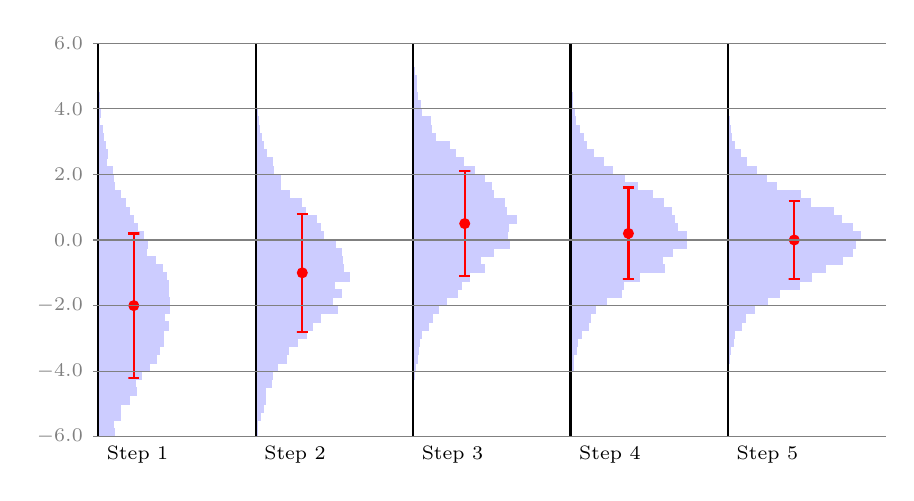
\begin{tikzpicture}[]
\begin{scope}[shift={(0.0,0.0)}]
\pgfsetxvec{\pgfpoint{0.002cm}{0cm}}
\pgfsetyvec{\pgfpoint{0cm}{0.41666666cm}}
\begin{scope}[shift={(-0.0,6.0)}]
\begin{scope}[fill=blue!20,draw=blue!20]
\pgfpathmoveto{ \pgfpointxy {0.0} {6.0}}
\pgfpathlineto{ \pgfpointxy {0.0} {6.0}}
\pgfpathlineto{ \pgfpointxy {0.0} {6.0}}
\pgfpathlineto{ \pgfpointxy {0.0} {5.75}}
\pgfpathlineto{ \pgfpointxy {1.0} {5.75}}
\pgfpathlineto{ \pgfpointxy {1.0} {5.5}}
\pgfpathlineto{ \pgfpointxy {0.0} {5.5}}
\pgfpathlineto{ \pgfpointxy {0.0} {5.25}}
\pgfpathlineto{ \pgfpointxy {2.0} {5.25}}
\pgfpathlineto{ \pgfpointxy {2.0} {5.0}}
\pgfpathlineto{ \pgfpointxy {5.0} {5.0}}
\pgfpathlineto{ \pgfpointxy {5.0} {4.75}}
\pgfpathlineto{ \pgfpointxy {5.0} {4.75}}
\pgfpathlineto{ \pgfpointxy {5.0} {4.5}}
\pgfpathlineto{ \pgfpointxy {8.0} {4.5}}
\pgfpathlineto{ \pgfpointxy {8.0} {4.25}}
\pgfpathlineto{ \pgfpointxy {9.0} {4.25}}
\pgfpathlineto{ \pgfpointxy {9.0} {4.0}}
\pgfpathlineto{ \pgfpointxy {12.0} {4.0}}
\pgfpathlineto{ \pgfpointxy {12.0} {3.75}}
\pgfpathlineto{ \pgfpointxy {9.0} {3.75}}
\pgfpathlineto{ \pgfpointxy {9.0} {3.5}}
\pgfpathlineto{ \pgfpointxy {28.0} {3.5}}
\pgfpathlineto{ \pgfpointxy {28.0} {3.25}}
\pgfpathlineto{ \pgfpointxy {35.0} {3.25}}
\pgfpathlineto{ \pgfpointxy {35.0} {3.0}}
\pgfpathlineto{ \pgfpointxy {45.0} {3.0}}
\pgfpathlineto{ \pgfpointxy {45.0} {2.75}}
\pgfpathlineto{ \pgfpointxy {58.0} {2.75}}
\pgfpathlineto{ \pgfpointxy {58.0} {2.5}}
\pgfpathlineto{ \pgfpointxy {53.0} {2.5}}
\pgfpathlineto{ \pgfpointxy {53.0} {2.25}}
\pgfpathlineto{ \pgfpointxy {90.0} {2.25}}
\pgfpathlineto{ \pgfpointxy {90.0} {2.0}}
\pgfpathlineto{ \pgfpointxy {95.0} {2.0}}
\pgfpathlineto{ \pgfpointxy {95.0} {1.75}}
\pgfpathlineto{ \pgfpointxy {102.0} {1.75}}
\pgfpathlineto{ \pgfpointxy {102.0} {1.5}}
\pgfpathlineto{ \pgfpointxy {144.0} {1.5}}
\pgfpathlineto{ \pgfpointxy {144.0} {1.25}}
\pgfpathlineto{ \pgfpointxy {175.0} {1.25}}
\pgfpathlineto{ \pgfpointxy {175.0} {1.0}}
\pgfpathlineto{ \pgfpointxy {202.0} {1.0}}
\pgfpathlineto{ \pgfpointxy {202.0} {0.75}}
\pgfpathlineto{ \pgfpointxy {224.0} {0.75}}
\pgfpathlineto{ \pgfpointxy {224.0} {0.5}}
\pgfpathlineto{ \pgfpointxy {250.0} {0.5}}
\pgfpathlineto{ \pgfpointxy {250.0} {0.25}}
\pgfpathlineto{ \pgfpointxy {285.0} {0.25}}
\pgfpathlineto{ \pgfpointxy {285.0} {0.0}}
\pgfpathlineto{ \pgfpointxy {316.0} {0.0}}
\pgfpathlineto{ \pgfpointxy {316.0} {-0.25}}
\pgfpathlineto{ \pgfpointxy {306.0} {-0.25}}
\pgfpathlineto{ \pgfpointxy {306.0} {-0.5}}
\pgfpathlineto{ \pgfpointxy {362.0} {-0.5}}
\pgfpathlineto{ \pgfpointxy {362.0} {-0.75}}
\pgfpathlineto{ \pgfpointxy {406.0} {-0.75}}
\pgfpathlineto{ \pgfpointxy {406.0} {-1.0}}
\pgfpathlineto{ \pgfpointxy {434.0} {-1.0}}
\pgfpathlineto{ \pgfpointxy {434.0} {-1.25}}
\pgfpathlineto{ \pgfpointxy {445.0} {-1.25}}
\pgfpathlineto{ \pgfpointxy {445.0} {-1.5}}
\pgfpathlineto{ \pgfpointxy {447.0} {-1.5}}
\pgfpathlineto{ \pgfpointxy {447.0} {-1.75}}
\pgfpathlineto{ \pgfpointxy {453.0} {-1.75}}
\pgfpathlineto{ \pgfpointxy {453.0} {-2.0}}
\pgfpathlineto{ \pgfpointxy {453.0} {-2.0}}
\pgfpathlineto{ \pgfpointxy {453.0} {-2.25}}
\pgfpathlineto{ \pgfpointxy {422.0} {-2.25}}
\pgfpathlineto{ \pgfpointxy {422.0} {-2.5}}
\pgfpathlineto{ \pgfpointxy {447.0} {-2.5}}
\pgfpathlineto{ \pgfpointxy {447.0} {-2.75}}
\pgfpathlineto{ \pgfpointxy {414.0} {-2.75}}
\pgfpathlineto{ \pgfpointxy {414.0} {-3.0}}
\pgfpathlineto{ \pgfpointxy {413.0} {-3.0}}
\pgfpathlineto{ \pgfpointxy {413.0} {-3.25}}
\pgfpathlineto{ \pgfpointxy {391.0} {-3.25}}
\pgfpathlineto{ \pgfpointxy {391.0} {-3.5}}
\pgfpathlineto{ \pgfpointxy {368.0} {-3.5}}
\pgfpathlineto{ \pgfpointxy {368.0} {-3.75}}
\pgfpathlineto{ \pgfpointxy {323.0} {-3.75}}
\pgfpathlineto{ \pgfpointxy {323.0} {-4.0}}
\pgfpathlineto{ \pgfpointxy {278.0} {-4.0}}
\pgfpathlineto{ \pgfpointxy {278.0} {-4.25}}
\pgfpathlineto{ \pgfpointxy {237.0} {-4.25}}
\pgfpathlineto{ \pgfpointxy {237.0} {-4.5}}
\pgfpathlineto{ \pgfpointxy {242.0} {-4.5}}
\pgfpathlineto{ \pgfpointxy {242.0} {-4.75}}
\pgfpathlineto{ \pgfpointxy {197.0} {-4.75}}
\pgfpathlineto{ \pgfpointxy {197.0} {-5.0}}
\pgfpathlineto{ \pgfpointxy {143.0} {-5.0}}
\pgfpathlineto{ \pgfpointxy {143.0} {-5.25}}
\pgfpathlineto{ \pgfpointxy {143.0} {-5.25}}
\pgfpathlineto{ \pgfpointxy {143.0} {-5.5}}
\pgfpathlineto{ \pgfpointxy {99.0} {-5.5}}
\pgfpathlineto{ \pgfpointxy {99.0} {-5.75}}
\pgfpathlineto{ \pgfpointxy {103.0} {-5.75}}
\pgfpathlineto{ \pgfpointxy {103.0} {-6.0}}
\pgfpathlineto{ \pgfpointxy {0.0} {-6.0}}
\pgfusepath{ stroke, fill, }
\end{scope}
\draw[thick,black] (0.0,-6.0) -- (0.0,6.0);
\begin{scope}[red,fill=red,thick]
\pgfpathmoveto{ \pgfpointadd{\pgfpointxy {226.5} {0.20000005}} {\pgfpoint{-2pt}{0}} }
\pgfpathlineto{ \pgfpointadd{\pgfpointxy {226.5} {0.20000005}} {\pgfpoint{2pt}{0}} }
\pgfpathlineto{ \pgfpointadd{\pgfpointxy {226.5} {0.20000005}} {\pgfpoint{0pt}{0}} }
\pgfpathlineto{ \pgfpointadd{\pgfpointxy {226.5} {-4.2}} {\pgfpoint{0pt}{0}} }
\pgfpathlineto{ \pgfpointadd{\pgfpointxy {226.5} {-4.2}} {\pgfpoint{-2pt}{0}} }
\pgfpathlineto{ \pgfpointadd{\pgfpointxy {226.5} {-4.2}} {\pgfpoint{2pt}{0}} }
\pgfusepath{ stroke, }
\node at (226.5,-2.0) [red,fill=red,thick,circle,inner sep=0.0pt,minimum width =4.0pt,minimum height=4.0pt] {};
\end{scope}
\end{scope}
\pgfsetxvec{\pgfpoint{1cm}{0cm}}
\pgfsetyvec{\pgfpoint{0cm}{1cm}}
\end{scope}
\begin{scope}[shift={(2.0,0.0)}]
\pgfsetxvec{\pgfpoint{0.002cm}{0cm}}
\pgfsetyvec{\pgfpoint{0cm}{0.41666666cm}}
\begin{scope}[shift={(-0.0,6.0)}]
\begin{scope}[fill=blue!20,draw=blue!20]
\pgfpathmoveto{ \pgfpointxy {0.0} {6.0}}
\pgfpathlineto{ \pgfpointxy {0.0} {6.0}}
\pgfpathlineto{ \pgfpointxy {0.0} {6.0}}
\pgfpathlineto{ \pgfpointxy {0.0} {5.75}}
\pgfpathlineto{ \pgfpointxy {3.0} {5.75}}
\pgfpathlineto{ \pgfpointxy {3.0} {5.5}}
\pgfpathlineto{ \pgfpointxy {3.0} {5.5}}
\pgfpathlineto{ \pgfpointxy {3.0} {5.25}}
\pgfpathlineto{ \pgfpointxy {2.0} {5.25}}
\pgfpathlineto{ \pgfpointxy {2.0} {5.0}}
\pgfpathlineto{ \pgfpointxy {4.0} {5.0}}
\pgfpathlineto{ \pgfpointxy {4.0} {4.75}}
\pgfpathlineto{ \pgfpointxy {4.0} {4.75}}
\pgfpathlineto{ \pgfpointxy {4.0} {4.5}}
\pgfpathlineto{ \pgfpointxy {7.0} {4.5}}
\pgfpathlineto{ \pgfpointxy {7.0} {4.25}}
\pgfpathlineto{ \pgfpointxy {7.0} {4.25}}
\pgfpathlineto{ \pgfpointxy {7.0} {4.0}}
\pgfpathlineto{ \pgfpointxy {13.0} {4.0}}
\pgfpathlineto{ \pgfpointxy {13.0} {3.75}}
\pgfpathlineto{ \pgfpointxy {20.0} {3.75}}
\pgfpathlineto{ \pgfpointxy {20.0} {3.5}}
\pgfpathlineto{ \pgfpointxy {23.0} {3.5}}
\pgfpathlineto{ \pgfpointxy {23.0} {3.25}}
\pgfpathlineto{ \pgfpointxy {35.0} {3.25}}
\pgfpathlineto{ \pgfpointxy {35.0} {3.0}}
\pgfpathlineto{ \pgfpointxy {47.0} {3.0}}
\pgfpathlineto{ \pgfpointxy {47.0} {2.75}}
\pgfpathlineto{ \pgfpointxy {71.0} {2.75}}
\pgfpathlineto{ \pgfpointxy {71.0} {2.5}}
\pgfpathlineto{ \pgfpointxy {104.0} {2.5}}
\pgfpathlineto{ \pgfpointxy {104.0} {2.25}}
\pgfpathlineto{ \pgfpointxy {112.0} {2.25}}
\pgfpathlineto{ \pgfpointxy {112.0} {2.0}}
\pgfpathlineto{ \pgfpointxy {156.0} {2.0}}
\pgfpathlineto{ \pgfpointxy {156.0} {1.75}}
\pgfpathlineto{ \pgfpointxy {159.0} {1.75}}
\pgfpathlineto{ \pgfpointxy {159.0} {1.5}}
\pgfpathlineto{ \pgfpointxy {218.0} {1.5}}
\pgfpathlineto{ \pgfpointxy {218.0} {1.25}}
\pgfpathlineto{ \pgfpointxy {288.0} {1.25}}
\pgfpathlineto{ \pgfpointxy {288.0} {1.0}}
\pgfpathlineto{ \pgfpointxy {314.0} {1.0}}
\pgfpathlineto{ \pgfpointxy {314.0} {0.75}}
\pgfpathlineto{ \pgfpointxy {388.0} {0.75}}
\pgfpathlineto{ \pgfpointxy {388.0} {0.5}}
\pgfpathlineto{ \pgfpointxy {414.0} {0.5}}
\pgfpathlineto{ \pgfpointxy {414.0} {0.25}}
\pgfpathlineto{ \pgfpointxy {428.0} {0.25}}
\pgfpathlineto{ \pgfpointxy {428.0} {0.0}}
\pgfpathlineto{ \pgfpointxy {510.0} {0.0}}
\pgfpathlineto{ \pgfpointxy {510.0} {-0.25}}
\pgfpathlineto{ \pgfpointxy {544.0} {-0.25}}
\pgfpathlineto{ \pgfpointxy {544.0} {-0.5}}
\pgfpathlineto{ \pgfpointxy {552.0} {-0.5}}
\pgfpathlineto{ \pgfpointxy {552.0} {-0.75}}
\pgfpathlineto{ \pgfpointxy {560.0} {-0.75}}
\pgfpathlineto{ \pgfpointxy {560.0} {-1.0}}
\pgfpathlineto{ \pgfpointxy {593.0} {-1.0}}
\pgfpathlineto{ \pgfpointxy {593.0} {-1.25}}
\pgfpathlineto{ \pgfpointxy {500.0} {-1.25}}
\pgfpathlineto{ \pgfpointxy {500.0} {-1.5}}
\pgfpathlineto{ \pgfpointxy {544.0} {-1.5}}
\pgfpathlineto{ \pgfpointxy {544.0} {-1.75}}
\pgfpathlineto{ \pgfpointxy {488.0} {-1.75}}
\pgfpathlineto{ \pgfpointxy {488.0} {-2.0}}
\pgfpathlineto{ \pgfpointxy {517.0} {-2.0}}
\pgfpathlineto{ \pgfpointxy {517.0} {-2.25}}
\pgfpathlineto{ \pgfpointxy {413.0} {-2.25}}
\pgfpathlineto{ \pgfpointxy {413.0} {-2.5}}
\pgfpathlineto{ \pgfpointxy {364.0} {-2.5}}
\pgfpathlineto{ \pgfpointxy {364.0} {-2.75}}
\pgfpathlineto{ \pgfpointxy {321.0} {-2.75}}
\pgfpathlineto{ \pgfpointxy {321.0} {-3.0}}
\pgfpathlineto{ \pgfpointxy {267.0} {-3.0}}
\pgfpathlineto{ \pgfpointxy {267.0} {-3.25}}
\pgfpathlineto{ \pgfpointxy {208.0} {-3.25}}
\pgfpathlineto{ \pgfpointxy {208.0} {-3.5}}
\pgfpathlineto{ \pgfpointxy {195.0} {-3.5}}
\pgfpathlineto{ \pgfpointxy {195.0} {-3.75}}
\pgfpathlineto{ \pgfpointxy {139.0} {-3.75}}
\pgfpathlineto{ \pgfpointxy {139.0} {-4.0}}
\pgfpathlineto{ \pgfpointxy {108.0} {-4.0}}
\pgfpathlineto{ \pgfpointxy {108.0} {-4.25}}
\pgfpathlineto{ \pgfpointxy {103.0} {-4.25}}
\pgfpathlineto{ \pgfpointxy {103.0} {-4.5}}
\pgfpathlineto{ \pgfpointxy {63.0} {-4.5}}
\pgfpathlineto{ \pgfpointxy {63.0} {-4.75}}
\pgfpathlineto{ \pgfpointxy {62.0} {-4.75}}
\pgfpathlineto{ \pgfpointxy {62.0} {-5.0}}
\pgfpathlineto{ \pgfpointxy {49.0} {-5.0}}
\pgfpathlineto{ \pgfpointxy {49.0} {-5.25}}
\pgfpathlineto{ \pgfpointxy {32.0} {-5.25}}
\pgfpathlineto{ \pgfpointxy {32.0} {-5.5}}
\pgfpathlineto{ \pgfpointxy {11.0} {-5.5}}
\pgfpathlineto{ \pgfpointxy {11.0} {-5.75}}
\pgfpathlineto{ \pgfpointxy {9.0} {-5.75}}
\pgfpathlineto{ \pgfpointxy {9.0} {-6.0}}
\pgfpathlineto{ \pgfpointxy {0.0} {-6.0}}
\pgfusepath{ stroke, fill, }
\end{scope}
\draw[thick,black] (0.0,-6.0) -- (0.0,6.0);
\begin{scope}[red,fill=red,thick]
\pgfpathmoveto{ \pgfpointadd{\pgfpointxy {296.5} {0.79999995}} {\pgfpoint{-2pt}{0}} }
\pgfpathlineto{ \pgfpointadd{\pgfpointxy {296.5} {0.79999995}} {\pgfpoint{2pt}{0}} }
\pgfpathlineto{ \pgfpointadd{\pgfpointxy {296.5} {0.79999995}} {\pgfpoint{0pt}{0}} }
\pgfpathlineto{ \pgfpointadd{\pgfpointxy {296.5} {-2.8}} {\pgfpoint{0pt}{0}} }
\pgfpathlineto{ \pgfpointadd{\pgfpointxy {296.5} {-2.8}} {\pgfpoint{-2pt}{0}} }
\pgfpathlineto{ \pgfpointadd{\pgfpointxy {296.5} {-2.8}} {\pgfpoint{2pt}{0}} }
\pgfusepath{ stroke, }
\node at (296.5,-1.0) [red,fill=red,thick,circle,inner sep=0.0pt,minimum width =4.0pt,minimum height=4.0pt] {};
\end{scope}
\end{scope}
\pgfsetxvec{\pgfpoint{1cm}{0cm}}
\pgfsetyvec{\pgfpoint{0cm}{1cm}}
\end{scope}
\begin{scope}[shift={(4.0,0.0)}]
\pgfsetxvec{\pgfpoint{0.002cm}{0cm}}
\pgfsetyvec{\pgfpoint{0cm}{0.41666666cm}}
\begin{scope}[shift={(-0.0,6.0)}]
\begin{scope}[fill=blue!20,draw=blue!20]
\pgfpathmoveto{ \pgfpointxy {0.0} {6.0}}
\pgfpathlineto{ \pgfpointxy {2.0} {6.0}}
\pgfpathlineto{ \pgfpointxy {2.0} {6.0}}
\pgfpathlineto{ \pgfpointxy {2.0} {5.75}}
\pgfpathlineto{ \pgfpointxy {3.0} {5.75}}
\pgfpathlineto{ \pgfpointxy {3.0} {5.5}}
\pgfpathlineto{ \pgfpointxy {5.0} {5.5}}
\pgfpathlineto{ \pgfpointxy {5.0} {5.25}}
\pgfpathlineto{ \pgfpointxy {9.0} {5.25}}
\pgfpathlineto{ \pgfpointxy {9.0} {5.0}}
\pgfpathlineto{ \pgfpointxy {21.0} {5.0}}
\pgfpathlineto{ \pgfpointxy {21.0} {4.75}}
\pgfpathlineto{ \pgfpointxy {19.0} {4.75}}
\pgfpathlineto{ \pgfpointxy {19.0} {4.5}}
\pgfpathlineto{ \pgfpointxy {26.0} {4.5}}
\pgfpathlineto{ \pgfpointxy {26.0} {4.25}}
\pgfpathlineto{ \pgfpointxy {47.0} {4.25}}
\pgfpathlineto{ \pgfpointxy {47.0} {4.0}}
\pgfpathlineto{ \pgfpointxy {52.0} {4.0}}
\pgfpathlineto{ \pgfpointxy {52.0} {3.75}}
\pgfpathlineto{ \pgfpointxy {108.0} {3.75}}
\pgfpathlineto{ \pgfpointxy {108.0} {3.5}}
\pgfpathlineto{ \pgfpointxy {116.0} {3.5}}
\pgfpathlineto{ \pgfpointxy {116.0} {3.25}}
\pgfpathlineto{ \pgfpointxy {145.0} {3.25}}
\pgfpathlineto{ \pgfpointxy {145.0} {3.0}}
\pgfpathlineto{ \pgfpointxy {229.0} {3.0}}
\pgfpathlineto{ \pgfpointxy {229.0} {2.75}}
\pgfpathlineto{ \pgfpointxy {267.0} {2.75}}
\pgfpathlineto{ \pgfpointxy {267.0} {2.5}}
\pgfpathlineto{ \pgfpointxy {323.0} {2.5}}
\pgfpathlineto{ \pgfpointxy {323.0} {2.25}}
\pgfpathlineto{ \pgfpointxy {391.0} {2.25}}
\pgfpathlineto{ \pgfpointxy {391.0} {2.0}}
\pgfpathlineto{ \pgfpointxy {455.0} {2.0}}
\pgfpathlineto{ \pgfpointxy {455.0} {1.75}}
\pgfpathlineto{ \pgfpointxy {496.0} {1.75}}
\pgfpathlineto{ \pgfpointxy {496.0} {1.5}}
\pgfpathlineto{ \pgfpointxy {511.0} {1.5}}
\pgfpathlineto{ \pgfpointxy {511.0} {1.25}}
\pgfpathlineto{ \pgfpointxy {583.0} {1.25}}
\pgfpathlineto{ \pgfpointxy {583.0} {1.0}}
\pgfpathlineto{ \pgfpointxy {593.0} {1.0}}
\pgfpathlineto{ \pgfpointxy {593.0} {0.75}}
\pgfpathlineto{ \pgfpointxy {656.0} {0.75}}
\pgfpathlineto{ \pgfpointxy {656.0} {0.5}}
\pgfpathlineto{ \pgfpointxy {604.0} {0.5}}
\pgfpathlineto{ \pgfpointxy {604.0} {0.25}}
\pgfpathlineto{ \pgfpointxy {600.0} {0.25}}
\pgfpathlineto{ \pgfpointxy {600.0} {0.0}}
\pgfpathlineto{ \pgfpointxy {610.0} {0.0}}
\pgfpathlineto{ \pgfpointxy {610.0} {-0.25}}
\pgfpathlineto{ \pgfpointxy {512.0} {-0.25}}
\pgfpathlineto{ \pgfpointxy {512.0} {-0.5}}
\pgfpathlineto{ \pgfpointxy {430.0} {-0.5}}
\pgfpathlineto{ \pgfpointxy {430.0} {-0.75}}
\pgfpathlineto{ \pgfpointxy {453.0} {-0.75}}
\pgfpathlineto{ \pgfpointxy {453.0} {-1.0}}
\pgfpathlineto{ \pgfpointxy {359.0} {-1.0}}
\pgfpathlineto{ \pgfpointxy {359.0} {-1.25}}
\pgfpathlineto{ \pgfpointxy {306.0} {-1.25}}
\pgfpathlineto{ \pgfpointxy {306.0} {-1.5}}
\pgfpathlineto{ \pgfpointxy {279.0} {-1.5}}
\pgfpathlineto{ \pgfpointxy {279.0} {-1.75}}
\pgfpathlineto{ \pgfpointxy {214.0} {-1.75}}
\pgfpathlineto{ \pgfpointxy {214.0} {-2.0}}
\pgfpathlineto{ \pgfpointxy {159.0} {-2.0}}
\pgfpathlineto{ \pgfpointxy {159.0} {-2.25}}
\pgfpathlineto{ \pgfpointxy {124.0} {-2.25}}
\pgfpathlineto{ \pgfpointxy {124.0} {-2.5}}
\pgfpathlineto{ \pgfpointxy {96.0} {-2.5}}
\pgfpathlineto{ \pgfpointxy {96.0} {-2.75}}
\pgfpathlineto{ \pgfpointxy {56.0} {-2.75}}
\pgfpathlineto{ \pgfpointxy {56.0} {-3.0}}
\pgfpathlineto{ \pgfpointxy {39.0} {-3.0}}
\pgfpathlineto{ \pgfpointxy {39.0} {-3.25}}
\pgfpathlineto{ \pgfpointxy {32.0} {-3.25}}
\pgfpathlineto{ \pgfpointxy {32.0} {-3.5}}
\pgfpathlineto{ \pgfpointxy {30.0} {-3.5}}
\pgfpathlineto{ \pgfpointxy {30.0} {-3.75}}
\pgfpathlineto{ \pgfpointxy {16.0} {-3.75}}
\pgfpathlineto{ \pgfpointxy {16.0} {-4.0}}
\pgfpathlineto{ \pgfpointxy {9.0} {-4.0}}
\pgfpathlineto{ \pgfpointxy {9.0} {-4.25}}
\pgfpathlineto{ \pgfpointxy {5.0} {-4.25}}
\pgfpathlineto{ \pgfpointxy {5.0} {-4.5}}
\pgfpathlineto{ \pgfpointxy {2.0} {-4.5}}
\pgfpathlineto{ \pgfpointxy {2.0} {-4.75}}
\pgfpathlineto{ \pgfpointxy {2.0} {-4.75}}
\pgfpathlineto{ \pgfpointxy {2.0} {-5.0}}
\pgfpathlineto{ \pgfpointxy {0.0} {-5.0}}
\pgfpathlineto{ \pgfpointxy {0.0} {-5.25}}
\pgfpathlineto{ \pgfpointxy {0.0} {-5.25}}
\pgfpathlineto{ \pgfpointxy {0.0} {-5.5}}
\pgfpathlineto{ \pgfpointxy {0.0} {-5.5}}
\pgfpathlineto{ \pgfpointxy {0.0} {-5.75}}
\pgfpathlineto{ \pgfpointxy {0.0} {-5.75}}
\pgfpathlineto{ \pgfpointxy {0.0} {-6.0}}
\pgfpathlineto{ \pgfpointxy {0.0} {-6.0}}
\pgfusepath{ stroke, fill, }
\end{scope}
\draw[thick,black] (0.0,-6.0) -- (0.0,6.0);
\begin{scope}[red,fill=red,thick]
\pgfpathmoveto{ \pgfpointadd{\pgfpointxy {328.0} {2.1}} {\pgfpoint{-2pt}{0}} }
\pgfpathlineto{ \pgfpointadd{\pgfpointxy {328.0} {2.1}} {\pgfpoint{2pt}{0}} }
\pgfpathlineto{ \pgfpointadd{\pgfpointxy {328.0} {2.1}} {\pgfpoint{0pt}{0}} }
\pgfpathlineto{ \pgfpointadd{\pgfpointxy {328.0} {-1.1}} {\pgfpoint{0pt}{0}} }
\pgfpathlineto{ \pgfpointadd{\pgfpointxy {328.0} {-1.1}} {\pgfpoint{-2pt}{0}} }
\pgfpathlineto{ \pgfpointadd{\pgfpointxy {328.0} {-1.1}} {\pgfpoint{2pt}{0}} }
\pgfusepath{ stroke, }
\node at (328.0,0.5) [red,fill=red,thick,circle,inner sep=0.0pt,minimum width =4.0pt,minimum height=4.0pt] {};
\end{scope}
\end{scope}
\pgfsetxvec{\pgfpoint{1cm}{0cm}}
\pgfsetyvec{\pgfpoint{0cm}{1cm}}
\end{scope}
\begin{scope}[shift={(6.0,0.0)}]
\pgfsetxvec{\pgfpoint{0.002cm}{0cm}}
\pgfsetyvec{\pgfpoint{0cm}{0.41666666cm}}
\begin{scope}[shift={(-0.0,6.0)}]
\begin{scope}[fill=blue!20,draw=blue!20]
\pgfpathmoveto{ \pgfpointxy {0.0} {6.0}}
\pgfpathlineto{ \pgfpointxy {0.0} {6.0}}
\pgfpathlineto{ \pgfpointxy {0.0} {6.0}}
\pgfpathlineto{ \pgfpointxy {0.0} {5.75}}
\pgfpathlineto{ \pgfpointxy {2.0} {5.75}}
\pgfpathlineto{ \pgfpointxy {2.0} {5.5}}
\pgfpathlineto{ \pgfpointxy {0.0} {5.5}}
\pgfpathlineto{ \pgfpointxy {0.0} {5.25}}
\pgfpathlineto{ \pgfpointxy {1.0} {5.25}}
\pgfpathlineto{ \pgfpointxy {1.0} {5.0}}
\pgfpathlineto{ \pgfpointxy {3.0} {5.0}}
\pgfpathlineto{ \pgfpointxy {3.0} {4.75}}
\pgfpathlineto{ \pgfpointxy {3.0} {4.75}}
\pgfpathlineto{ \pgfpointxy {3.0} {4.5}}
\pgfpathlineto{ \pgfpointxy {10.0} {4.5}}
\pgfpathlineto{ \pgfpointxy {10.0} {4.25}}
\pgfpathlineto{ \pgfpointxy {13.0} {4.25}}
\pgfpathlineto{ \pgfpointxy {13.0} {4.0}}
\pgfpathlineto{ \pgfpointxy {22.0} {4.0}}
\pgfpathlineto{ \pgfpointxy {22.0} {3.75}}
\pgfpathlineto{ \pgfpointxy {28.0} {3.75}}
\pgfpathlineto{ \pgfpointxy {28.0} {3.5}}
\pgfpathlineto{ \pgfpointxy {58.0} {3.5}}
\pgfpathlineto{ \pgfpointxy {58.0} {3.25}}
\pgfpathlineto{ \pgfpointxy {81.0} {3.25}}
\pgfpathlineto{ \pgfpointxy {81.0} {3.0}}
\pgfpathlineto{ \pgfpointxy {99.0} {3.0}}
\pgfpathlineto{ \pgfpointxy {99.0} {2.75}}
\pgfpathlineto{ \pgfpointxy {146.0} {2.75}}
\pgfpathlineto{ \pgfpointxy {146.0} {2.5}}
\pgfpathlineto{ \pgfpointxy {209.0} {2.5}}
\pgfpathlineto{ \pgfpointxy {209.0} {2.25}}
\pgfpathlineto{ \pgfpointxy {265.0} {2.25}}
\pgfpathlineto{ \pgfpointxy {265.0} {2.0}}
\pgfpathlineto{ \pgfpointxy {341.0} {2.0}}
\pgfpathlineto{ \pgfpointxy {341.0} {1.75}}
\pgfpathlineto{ \pgfpointxy {424.0} {1.75}}
\pgfpathlineto{ \pgfpointxy {424.0} {1.5}}
\pgfpathlineto{ \pgfpointxy {522.0} {1.5}}
\pgfpathlineto{ \pgfpointxy {522.0} {1.25}}
\pgfpathlineto{ \pgfpointxy {590.0} {1.25}}
\pgfpathlineto{ \pgfpointxy {590.0} {1.0}}
\pgfpathlineto{ \pgfpointxy {640.0} {1.0}}
\pgfpathlineto{ \pgfpointxy {640.0} {0.75}}
\pgfpathlineto{ \pgfpointxy {662.0} {0.75}}
\pgfpathlineto{ \pgfpointxy {662.0} {0.5}}
\pgfpathlineto{ \pgfpointxy {676.0} {0.5}}
\pgfpathlineto{ \pgfpointxy {676.0} {0.25}}
\pgfpathlineto{ \pgfpointxy {735.0} {0.25}}
\pgfpathlineto{ \pgfpointxy {735.0} {0.0}}
\pgfpathlineto{ \pgfpointxy {734.0} {0.0}}
\pgfpathlineto{ \pgfpointxy {734.0} {-0.25}}
\pgfpathlineto{ \pgfpointxy {647.0} {-0.25}}
\pgfpathlineto{ \pgfpointxy {647.0} {-0.5}}
\pgfpathlineto{ \pgfpointxy {585.0} {-0.5}}
\pgfpathlineto{ \pgfpointxy {585.0} {-0.75}}
\pgfpathlineto{ \pgfpointxy {594.0} {-0.75}}
\pgfpathlineto{ \pgfpointxy {594.0} {-1.0}}
\pgfpathlineto{ \pgfpointxy {438.0} {-1.0}}
\pgfpathlineto{ \pgfpointxy {438.0} {-1.25}}
\pgfpathlineto{ \pgfpointxy {338.0} {-1.25}}
\pgfpathlineto{ \pgfpointxy {338.0} {-1.5}}
\pgfpathlineto{ \pgfpointxy {323.0} {-1.5}}
\pgfpathlineto{ \pgfpointxy {323.0} {-1.75}}
\pgfpathlineto{ \pgfpointxy {228.0} {-1.75}}
\pgfpathlineto{ \pgfpointxy {228.0} {-2.0}}
\pgfpathlineto{ \pgfpointxy {161.0} {-2.0}}
\pgfpathlineto{ \pgfpointxy {161.0} {-2.25}}
\pgfpathlineto{ \pgfpointxy {124.0} {-2.25}}
\pgfpathlineto{ \pgfpointxy {124.0} {-2.5}}
\pgfpathlineto{ \pgfpointxy {116.0} {-2.5}}
\pgfpathlineto{ \pgfpointxy {116.0} {-2.75}}
\pgfpathlineto{ \pgfpointxy {69.0} {-2.75}}
\pgfpathlineto{ \pgfpointxy {69.0} {-3.0}}
\pgfpathlineto{ \pgfpointxy {42.0} {-3.0}}
\pgfpathlineto{ \pgfpointxy {42.0} {-3.25}}
\pgfpathlineto{ \pgfpointxy {35.0} {-3.25}}
\pgfpathlineto{ \pgfpointxy {35.0} {-3.5}}
\pgfpathlineto{ \pgfpointxy {15.0} {-3.5}}
\pgfpathlineto{ \pgfpointxy {15.0} {-3.75}}
\pgfpathlineto{ \pgfpointxy {15.0} {-3.75}}
\pgfpathlineto{ \pgfpointxy {15.0} {-4.0}}
\pgfpathlineto{ \pgfpointxy {3.0} {-4.0}}
\pgfpathlineto{ \pgfpointxy {3.0} {-4.25}}
\pgfpathlineto{ \pgfpointxy {2.0} {-4.25}}
\pgfpathlineto{ \pgfpointxy {2.0} {-4.5}}
\pgfpathlineto{ \pgfpointxy {0.0} {-4.5}}
\pgfpathlineto{ \pgfpointxy {0.0} {-4.75}}
\pgfpathlineto{ \pgfpointxy {0.0} {-4.75}}
\pgfpathlineto{ \pgfpointxy {0.0} {-5.0}}
\pgfpathlineto{ \pgfpointxy {0.0} {-5.0}}
\pgfpathlineto{ \pgfpointxy {0.0} {-5.25}}
\pgfpathlineto{ \pgfpointxy {0.0} {-5.25}}
\pgfpathlineto{ \pgfpointxy {0.0} {-5.5}}
\pgfpathlineto{ \pgfpointxy {0.0} {-5.5}}
\pgfpathlineto{ \pgfpointxy {0.0} {-5.75}}
\pgfpathlineto{ \pgfpointxy {0.0} {-5.75}}
\pgfpathlineto{ \pgfpointxy {0.0} {-6.0}}
\pgfpathlineto{ \pgfpointxy {0.0} {-6.0}}
\pgfusepath{ stroke, fill, }
\end{scope}
\draw[thick,black] (0.0,-6.0) -- (0.0,6.0);
\begin{scope}[red,fill=red,thick]
\pgfpathmoveto{ \pgfpointadd{\pgfpointxy {367.5} {1.6}} {\pgfpoint{-2pt}{0}} }
\pgfpathlineto{ \pgfpointadd{\pgfpointxy {367.5} {1.6}} {\pgfpoint{2pt}{0}} }
\pgfpathlineto{ \pgfpointadd{\pgfpointxy {367.5} {1.6}} {\pgfpoint{0pt}{0}} }
\pgfpathlineto{ \pgfpointadd{\pgfpointxy {367.5} {-1.1999999}} {\pgfpoint{0pt}{0}} }
\pgfpathlineto{ \pgfpointadd{\pgfpointxy {367.5} {-1.1999999}} {\pgfpoint{-2pt}{0}} }
\pgfpathlineto{ \pgfpointadd{\pgfpointxy {367.5} {-1.1999999}} {\pgfpoint{2pt}{0}} }
\pgfusepath{ stroke, }
\node at (367.5,0.2) [red,fill=red,thick,circle,inner sep=0.0pt,minimum width =4.0pt,minimum height=4.0pt] {};
\end{scope}
\end{scope}
\pgfsetxvec{\pgfpoint{1cm}{0cm}}
\pgfsetyvec{\pgfpoint{0cm}{1cm}}
\end{scope}
\begin{scope}[shift={(8.0,0.0)}]
\pgfsetxvec{\pgfpoint{0.002cm}{0cm}}
\pgfsetyvec{\pgfpoint{0cm}{0.41666666cm}}
\begin{scope}[shift={(-0.0,6.0)}]
\begin{scope}[fill=blue!20,draw=blue!20]
\pgfpathmoveto{ \pgfpointxy {0.0} {6.0}}
\pgfpathlineto{ \pgfpointxy {0.0} {6.0}}
\pgfpathlineto{ \pgfpointxy {0.0} {6.0}}
\pgfpathlineto{ \pgfpointxy {0.0} {5.75}}
\pgfpathlineto{ \pgfpointxy {0.0} {5.75}}
\pgfpathlineto{ \pgfpointxy {0.0} {5.5}}
\pgfpathlineto{ \pgfpointxy {0.0} {5.5}}
\pgfpathlineto{ \pgfpointxy {0.0} {5.25}}
\pgfpathlineto{ \pgfpointxy {0.0} {5.25}}
\pgfpathlineto{ \pgfpointxy {0.0} {5.0}}
\pgfpathlineto{ \pgfpointxy {0.0} {5.0}}
\pgfpathlineto{ \pgfpointxy {0.0} {4.75}}
\pgfpathlineto{ \pgfpointxy {2.0} {4.75}}
\pgfpathlineto{ \pgfpointxy {2.0} {4.5}}
\pgfpathlineto{ \pgfpointxy {1.0} {4.5}}
\pgfpathlineto{ \pgfpointxy {1.0} {4.25}}
\pgfpathlineto{ \pgfpointxy {1.0} {4.25}}
\pgfpathlineto{ \pgfpointxy {1.0} {4.0}}
\pgfpathlineto{ \pgfpointxy {4.0} {4.0}}
\pgfpathlineto{ \pgfpointxy {4.0} {3.75}}
\pgfpathlineto{ \pgfpointxy {8.0} {3.75}}
\pgfpathlineto{ \pgfpointxy {8.0} {3.5}}
\pgfpathlineto{ \pgfpointxy {17.0} {3.5}}
\pgfpathlineto{ \pgfpointxy {17.0} {3.25}}
\pgfpathlineto{ \pgfpointxy {24.0} {3.25}}
\pgfpathlineto{ \pgfpointxy {24.0} {3.0}}
\pgfpathlineto{ \pgfpointxy {43.0} {3.0}}
\pgfpathlineto{ \pgfpointxy {43.0} {2.75}}
\pgfpathlineto{ \pgfpointxy {81.0} {2.75}}
\pgfpathlineto{ \pgfpointxy {81.0} {2.5}}
\pgfpathlineto{ \pgfpointxy {116.0} {2.5}}
\pgfpathlineto{ \pgfpointxy {116.0} {2.25}}
\pgfpathlineto{ \pgfpointxy {182.0} {2.25}}
\pgfpathlineto{ \pgfpointxy {182.0} {2.0}}
\pgfpathlineto{ \pgfpointxy {247.0} {2.0}}
\pgfpathlineto{ \pgfpointxy {247.0} {1.75}}
\pgfpathlineto{ \pgfpointxy {307.0} {1.75}}
\pgfpathlineto{ \pgfpointxy {307.0} {1.5}}
\pgfpathlineto{ \pgfpointxy {463.0} {1.5}}
\pgfpathlineto{ \pgfpointxy {463.0} {1.25}}
\pgfpathlineto{ \pgfpointxy {521.0} {1.25}}
\pgfpathlineto{ \pgfpointxy {521.0} {1.0}}
\pgfpathlineto{ \pgfpointxy {671.0} {1.0}}
\pgfpathlineto{ \pgfpointxy {671.0} {0.75}}
\pgfpathlineto{ \pgfpointxy {723.0} {0.75}}
\pgfpathlineto{ \pgfpointxy {723.0} {0.5}}
\pgfpathlineto{ \pgfpointxy {789.0} {0.5}}
\pgfpathlineto{ \pgfpointxy {789.0} {0.25}}
\pgfpathlineto{ \pgfpointxy {841.0} {0.25}}
\pgfpathlineto{ \pgfpointxy {841.0} {0.0}}
\pgfpathlineto{ \pgfpointxy {810.0} {0.0}}
\pgfpathlineto{ \pgfpointxy {810.0} {-0.25}}
\pgfpathlineto{ \pgfpointxy {791.0} {-0.25}}
\pgfpathlineto{ \pgfpointxy {791.0} {-0.5}}
\pgfpathlineto{ \pgfpointxy {724.0} {-0.5}}
\pgfpathlineto{ \pgfpointxy {724.0} {-0.75}}
\pgfpathlineto{ \pgfpointxy {618.0} {-0.75}}
\pgfpathlineto{ \pgfpointxy {618.0} {-1.0}}
\pgfpathlineto{ \pgfpointxy {528.0} {-1.0}}
\pgfpathlineto{ \pgfpointxy {528.0} {-1.25}}
\pgfpathlineto{ \pgfpointxy {454.0} {-1.25}}
\pgfpathlineto{ \pgfpointxy {454.0} {-1.5}}
\pgfpathlineto{ \pgfpointxy {327.0} {-1.5}}
\pgfpathlineto{ \pgfpointxy {327.0} {-1.75}}
\pgfpathlineto{ \pgfpointxy {252.0} {-1.75}}
\pgfpathlineto{ \pgfpointxy {252.0} {-2.0}}
\pgfpathlineto{ \pgfpointxy {165.0} {-2.0}}
\pgfpathlineto{ \pgfpointxy {165.0} {-2.25}}
\pgfpathlineto{ \pgfpointxy {108.0} {-2.25}}
\pgfpathlineto{ \pgfpointxy {108.0} {-2.5}}
\pgfpathlineto{ \pgfpointxy {82.0} {-2.5}}
\pgfpathlineto{ \pgfpointxy {82.0} {-2.75}}
\pgfpathlineto{ \pgfpointxy {42.0} {-2.75}}
\pgfpathlineto{ \pgfpointxy {42.0} {-3.0}}
\pgfpathlineto{ \pgfpointxy {31.0} {-3.0}}
\pgfpathlineto{ \pgfpointxy {31.0} {-3.25}}
\pgfpathlineto{ \pgfpointxy {15.0} {-3.25}}
\pgfpathlineto{ \pgfpointxy {15.0} {-3.5}}
\pgfpathlineto{ \pgfpointxy {6.0} {-3.5}}
\pgfpathlineto{ \pgfpointxy {6.0} {-3.75}}
\pgfpathlineto{ \pgfpointxy {5.0} {-3.75}}
\pgfpathlineto{ \pgfpointxy {5.0} {-4.0}}
\pgfpathlineto{ \pgfpointxy {1.0} {-4.0}}
\pgfpathlineto{ \pgfpointxy {1.0} {-4.25}}
\pgfpathlineto{ \pgfpointxy {0.0} {-4.25}}
\pgfpathlineto{ \pgfpointxy {0.0} {-4.5}}
\pgfpathlineto{ \pgfpointxy {0.0} {-4.5}}
\pgfpathlineto{ \pgfpointxy {0.0} {-4.75}}
\pgfpathlineto{ \pgfpointxy {0.0} {-4.75}}
\pgfpathlineto{ \pgfpointxy {0.0} {-5.0}}
\pgfpathlineto{ \pgfpointxy {0.0} {-5.0}}
\pgfpathlineto{ \pgfpointxy {0.0} {-5.25}}
\pgfpathlineto{ \pgfpointxy {0.0} {-5.25}}
\pgfpathlineto{ \pgfpointxy {0.0} {-5.5}}
\pgfpathlineto{ \pgfpointxy {0.0} {-5.5}}
\pgfpathlineto{ \pgfpointxy {0.0} {-5.75}}
\pgfpathlineto{ \pgfpointxy {0.0} {-5.75}}
\pgfpathlineto{ \pgfpointxy {0.0} {-6.0}}
\pgfpathlineto{ \pgfpointxy {0.0} {-6.0}}
\pgfusepath{ stroke, fill, }
\end{scope}
\draw[thick,black] (0.0,-6.0) -- (0.0,6.0);
\begin{scope}[red,fill=red,thick]
\pgfpathmoveto{ \pgfpointadd{\pgfpointxy {420.5} {1.2}} {\pgfpoint{-2pt}{0}} }
\pgfpathlineto{ \pgfpointadd{\pgfpointxy {420.5} {1.2}} {\pgfpoint{2pt}{0}} }
\pgfpathlineto{ \pgfpointadd{\pgfpointxy {420.5} {1.2}} {\pgfpoint{0pt}{0}} }
\pgfpathlineto{ \pgfpointadd{\pgfpointxy {420.5} {-1.2}} {\pgfpoint{0pt}{0}} }
\pgfpathlineto{ \pgfpointadd{\pgfpointxy {420.5} {-1.2}} {\pgfpoint{-2pt}{0}} }
\pgfpathlineto{ \pgfpointadd{\pgfpointxy {420.5} {-1.2}} {\pgfpoint{2pt}{0}} }
\pgfusepath{ stroke, }
\node at (420.5,0.0) [red,fill=red,thick,circle,inner sep=0.0pt,minimum width =4.0pt,minimum height=4.0pt] {};
\end{scope}
\end{scope}
\pgfsetxvec{\pgfpoint{1cm}{0cm}}
\pgfsetyvec{\pgfpoint{0cm}{1cm}}
\end{scope}
\begin{scope}[shift={(0.0,0.0)}]
\pgfsetxvec{\pgfpoint{1.0cm}{0cm}}
\pgfsetyvec{\pgfpoint{0cm}{0.41666666cm}}
\begin{scope}[shift={(-0.0,6.0)}]
\begin{scope}[xshift=0cm]
\draw[gray] [shift={(0.0,-6.0)}] (10cm,0) -- (-2pt,0) node[left]{ \scriptsize{\num[round-mode=places,round-precision=1]{-6.0}}};
\draw[gray] [shift={(0.0,-4.0)}] (10cm,0) -- (-2pt,0) node[left]{ \scriptsize{\num[round-mode=places,round-precision=1]{-4.0}}};
\draw[gray] [shift={(0.0,-2.0)}] (10cm,0) -- (-2pt,0) node[left]{ \scriptsize{\num[round-mode=places,round-precision=1]{-2.0}}};
\draw[gray] [shift={(0.0,0.0)}] (10cm,0) -- (-2pt,0) node[left]{ \scriptsize{\num[round-mode=places,round-precision=1]{0.0}}};
\draw[gray] [shift={(0.0,2.0)}] (10cm,0) -- (-2pt,0) node[left]{ \scriptsize{\num[round-mode=places,round-precision=1]{2.0}}};
\draw[gray] [shift={(0.0,4.0)}] (10cm,0) -- (-2pt,0) node[left]{ \scriptsize{\num[round-mode=places,round-precision=1]{4.0}}};
\draw[gray] [shift={(0.0,6.0)}] (10cm,0) -- (-2pt,0) node[left]{ \scriptsize{\num[round-mode=places,round-precision=1]{6.0}}};
\end{scope}
\end{scope}
\pgfsetxvec{\pgfpoint{1cm}{0cm}}
\pgfsetyvec{\pgfpoint{0cm}{1cm}}
\end{scope}
\begin{scope}[shift={(0.0,0.0)}]
\pgfsetxvec{\pgfpoint{1.0cm}{0cm}}
\pgfsetyvec{\pgfpoint{0cm}{0.41666666cm}}
\begin{scope}[shift={(-0.0,6.0)}]
\begin{scope}[yshift=0cm]
\draw[black] [shift={(0.5,-6.0)}] (0,0) -- (0,0) node[below]{ \scriptsize{Step 1}};
\draw[black] [shift={(2.5,-6.0)}] (0,0) -- (0,0) node[below]{ \scriptsize{Step 2}};
\draw[black] [shift={(4.5,-6.0)}] (0,0) -- (0,0) node[below]{ \scriptsize{Step 3}};
\draw[black] [shift={(6.5,-6.0)}] (0,0) -- (0,0) node[below]{ \scriptsize{Step 4}};
\draw[black] [shift={(8.5,-6.0)}] (0,0) -- (0,0) node[below]{ \scriptsize{Step 5}};
\end{scope}
\end{scope}
\pgfsetxvec{\pgfpoint{1cm}{0cm}}
\pgfsetyvec{\pgfpoint{0cm}{1cm}}
\end{scope}
\end{tikzpicture}
\end{document}

\captionsetup{singlelinecheck=off}
\caption[asdf]{Horizontal histograms, in sub figures side by side. The mean and $\sigma$ are indicated in red.}
\end{figure}
\begin{figure}[H]
\centering
\documentclass{standalone}
\ifx\HCode\UnDef\else\def\pgfsysdriver{pgfsys-tex4ht.def}\fi
\usepackage{tikz}
\usepackage{color}
\usepackage{siunitx}
\usetikzlibrary{arrows,shapes}
\begin{document}
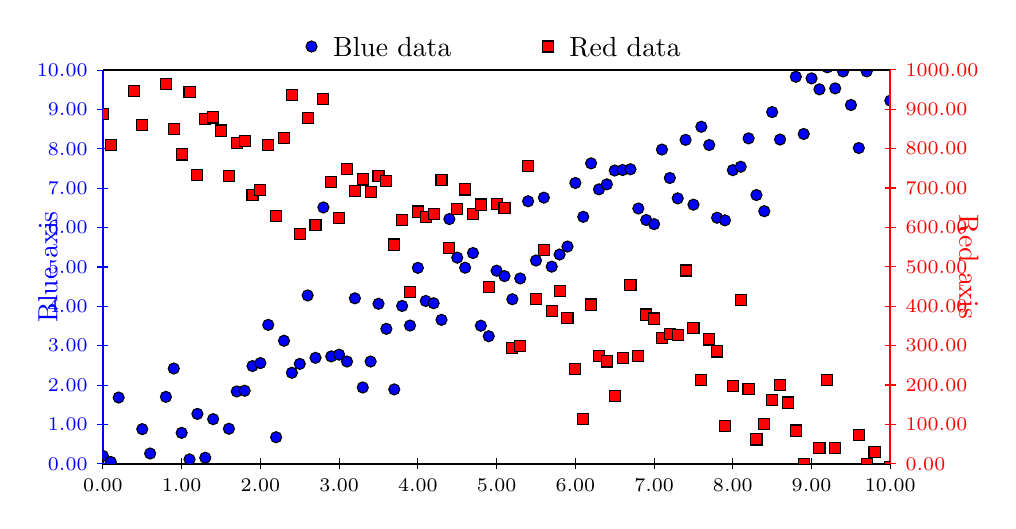
\begin{tikzpicture}
\draw[thick,black] (0.0,0.0) -- (10.0,0.0);
\draw[thick,blue] (0.0,0.0) -- (0.0,5.0);
\node[rotate=90,blue] at (-0.7,2.5) {Blue axis};
\begin{scope}[shift={(0.0,0.0)}]
\pgfsetxvec{\pgfpoint{1.0cm}{0cm}}
\pgfsetyvec{\pgfpoint{0cm}{0.5cm}}
\begin{scope}[shift={(0.0,0.0)}]
\begin{scope}[yshift=0cm]
\draw[black] [shift={(0.0,0.0)}] (0,2pt) -- (0,-2pt) node[below]{ \scriptsize{\num[round-mode=places,round-precision=2]{0}}};
\draw[black] [shift={(1.0,0.0)}] (0,2pt) -- (0,-2pt) node[below]{ \scriptsize{\num[round-mode=places,round-precision=2]{1}}};
\draw[black] [shift={(2.0,0.0)}] (0,2pt) -- (0,-2pt) node[below]{ \scriptsize{\num[round-mode=places,round-precision=2]{2}}};
\draw[black] [shift={(3.0,0.0)}] (0,2pt) -- (0,-2pt) node[below]{ \scriptsize{\num[round-mode=places,round-precision=2]{3}}};
\draw[black] [shift={(4.0,0.0)}] (0,2pt) -- (0,-2pt) node[below]{ \scriptsize{\num[round-mode=places,round-precision=2]{4}}};
\draw[black] [shift={(5.0,0.0)}] (0,2pt) -- (0,-2pt) node[below]{ \scriptsize{\num[round-mode=places,round-precision=2]{5}}};
\draw[black] [shift={(6.0,0.0)}] (0,2pt) -- (0,-2pt) node[below]{ \scriptsize{\num[round-mode=places,round-precision=2]{6}}};
\draw[black] [shift={(7.0,0.0)}] (0,2pt) -- (0,-2pt) node[below]{ \scriptsize{\num[round-mode=places,round-precision=2]{7}}};
\draw[black] [shift={(8.0,0.0)}] (0,2pt) -- (0,-2pt) node[below]{ \scriptsize{\num[round-mode=places,round-precision=2]{8}}};
\draw[black] [shift={(9.0,0.0)}] (0,2pt) -- (0,-2pt) node[below]{ \scriptsize{\num[round-mode=places,round-precision=2]{9}}};
\draw[black] [shift={(10.0,0.0)}] (0,2pt) -- (0,-2pt) node[below]{ \scriptsize{\num[round-mode=places,round-precision=2]{10}}};
\end{scope}
\begin{scope}[xshift=0cm]
\draw[blue] [shift={(0.0,0.0)}] (2pt,0) -- (-2pt,0) node[left]{ \scriptsize{\num[round-mode=places,round-precision=2]{0}}};
\draw[blue] [shift={(0.0,1.0)}] (2pt,0) -- (-2pt,0) node[left]{ \scriptsize{\num[round-mode=places,round-precision=2]{1}}};
\draw[blue] [shift={(0.0,2.0)}] (2pt,0) -- (-2pt,0) node[left]{ \scriptsize{\num[round-mode=places,round-precision=2]{2}}};
\draw[blue] [shift={(0.0,3.0)}] (2pt,0) -- (-2pt,0) node[left]{ \scriptsize{\num[round-mode=places,round-precision=2]{3}}};
\draw[blue] [shift={(0.0,4.0)}] (2pt,0) -- (-2pt,0) node[left]{ \scriptsize{\num[round-mode=places,round-precision=2]{4}}};
\draw[blue] [shift={(0.0,5.0)}] (2pt,0) -- (-2pt,0) node[left]{ \scriptsize{\num[round-mode=places,round-precision=2]{5}}};
\draw[blue] [shift={(0.0,6.0)}] (2pt,0) -- (-2pt,0) node[left]{ \scriptsize{\num[round-mode=places,round-precision=2]{6}}};
\draw[blue] [shift={(0.0,7.0)}] (2pt,0) -- (-2pt,0) node[left]{ \scriptsize{\num[round-mode=places,round-precision=2]{7}}};
\draw[blue] [shift={(0.0,8.0)}] (2pt,0) -- (-2pt,0) node[left]{ \scriptsize{\num[round-mode=places,round-precision=2]{8}}};
\draw[blue] [shift={(0.0,9.0)}] (2pt,0) -- (-2pt,0) node[left]{ \scriptsize{\num[round-mode=places,round-precision=2]{9}}};
\draw[blue] [shift={(0.0,10.0)}] (2pt,0) -- (-2pt,0) node[left]{ \scriptsize{\num[round-mode=places,round-precision=2]{10}}};
\end{scope}
\end{scope}
\pgfsetxvec{\pgfpoint{1cm}{0cm}}
\pgfsetyvec{\pgfpoint{0cm}{1cm}}
\end{scope}
\begin{scope}[]
\pgfpathmoveto{ \pgfpointxy {0.0} {0.0}}
\pgfpathlineto{ \pgfpointxy {10.0} {0.0}}
\pgfpathlineto{ \pgfpointxy {10.0} {5.0}}
\pgfpathlineto{ \pgfpointxy {0.0} {5.0}}
\pgfpathclose
\pgfusepath{  clip, }
\begin{scope}[shift={(0.0,0.0)}]
\pgfsetxvec{\pgfpoint{1.0cm}{0cm}}
\pgfsetyvec{\pgfpoint{0cm}{0.5cm}}
\begin{scope}[shift={(0.0,0.0)}]
\node at (0.0,0.2018202808197739) [circle,inner sep=0.0pt,minimum width =4.0pt,minimum height=4.0pt,draw=black,fill=blue] {}; 
\node at (0.1,0.04802957026620584) [circle,inner sep=0.0pt,minimum width =4.0pt,minimum height=4.0pt,draw=black,fill=blue] {}; 
\node at (0.2,1.6838771144268656) [circle,inner sep=0.0pt,minimum width =4.0pt,minimum height=4.0pt,draw=black,fill=blue] {}; 
\node at (0.3,-2.178869925168345) [circle,inner sep=0.0pt,minimum width =4.0pt,minimum height=4.0pt,draw=black,fill=blue] {}; 
\node at (0.4,-1.4007813471041273) [circle,inner sep=0.0pt,minimum width =4.0pt,minimum height=4.0pt,draw=black,fill=blue] {}; 
\node at (0.5,0.8810027621619783) [circle,inner sep=0.0pt,minimum width =4.0pt,minimum height=4.0pt,draw=black,fill=blue] {}; 
\node at (0.6,0.2622437423498728) [circle,inner sep=0.0pt,minimum width =4.0pt,minimum height=4.0pt,draw=black,fill=blue] {}; 
\node at (0.7,-0.99061855907404) [circle,inner sep=0.0pt,minimum width =4.0pt,minimum height=4.0pt,draw=black,fill=blue] {}; 
\node at (0.8,1.700983830337498) [circle,inner sep=0.0pt,minimum width =4.0pt,minimum height=4.0pt,draw=black,fill=blue] {}; 
\node at (0.90000004,2.4203191007601728) [circle,inner sep=0.0pt,minimum width =4.0pt,minimum height=4.0pt,draw=black,fill=blue] {}; 
\node at (1.0,0.7868319047053163) [circle,inner sep=0.0pt,minimum width =4.0pt,minimum height=4.0pt,draw=black,fill=blue] {}; 
\node at (1.1,0.11223198209833973) [circle,inner sep=0.0pt,minimum width =4.0pt,minimum height=4.0pt,draw=black,fill=blue] {}; 
\node at (1.2,1.2685385794326152) [circle,inner sep=0.0pt,minimum width =4.0pt,minimum height=4.0pt,draw=black,fill=blue] {}; 
\node at (1.3000001,0.15439379978621104) [circle,inner sep=0.0pt,minimum width =4.0pt,minimum height=4.0pt,draw=black,fill=blue] {}; 
\node at (1.4,1.1351089428880914) [circle,inner sep=0.0pt,minimum width =4.0pt,minimum height=4.0pt,draw=black,fill=blue] {}; 
\node at (1.5,-0.5000313320572731) [circle,inner sep=0.0pt,minimum width =4.0pt,minimum height=4.0pt,draw=black,fill=blue] {}; 
\node at (1.6,0.8905312794485365) [circle,inner sep=0.0pt,minimum width =4.0pt,minimum height=4.0pt,draw=black,fill=blue] {}; 
\node at (1.7,1.8385845366548643) [circle,inner sep=0.0pt,minimum width =4.0pt,minimum height=4.0pt,draw=black,fill=blue] {}; 
\node at (1.8000001,1.8566978002918142) [circle,inner sep=0.0pt,minimum width =4.0pt,minimum height=4.0pt,draw=black,fill=blue] {}; 
\node at (1.9,2.4839211368075533) [circle,inner sep=0.0pt,minimum width =4.0pt,minimum height=4.0pt,draw=black,fill=blue] {}; 
\node at (2.0,2.5583679978459055) [circle,inner sep=0.0pt,minimum width =4.0pt,minimum height=4.0pt,draw=black,fill=blue] {}; 
\node at (2.1000001,3.5298453509789764) [circle,inner sep=0.0pt,minimum width =4.0pt,minimum height=4.0pt,draw=black,fill=blue] {}; 
\node at (2.2,0.6756204600873008) [circle,inner sep=0.0pt,minimum width =4.0pt,minimum height=4.0pt,draw=black,fill=blue] {}; 
\node at (2.3,3.126374645219319) [circle,inner sep=0.0pt,minimum width =4.0pt,minimum height=4.0pt,draw=black,fill=blue] {}; 
\node at (2.4,2.3129840835702056) [circle,inner sep=0.0pt,minimum width =4.0pt,minimum height=4.0pt,draw=black,fill=blue] {}; 
\node at (2.5,2.5382451570068807) [circle,inner sep=0.0pt,minimum width =4.0pt,minimum height=4.0pt,draw=black,fill=blue] {}; 
\node at (2.6000001,4.277364693656243) [circle,inner sep=0.0pt,minimum width =4.0pt,minimum height=4.0pt,draw=black,fill=blue] {}; 
\node at (2.7,2.6928054801585852) [circle,inner sep=0.0pt,minimum width =4.0pt,minimum height=4.0pt,draw=black,fill=blue] {}; 
\node at (2.8,6.5119910434838335) [circle,inner sep=0.0pt,minimum width =4.0pt,minimum height=4.0pt,draw=black,fill=blue] {}; 
\node at (2.9,2.7291128416515873) [circle,inner sep=0.0pt,minimum width =4.0pt,minimum height=4.0pt,draw=black,fill=blue] {}; 
\node at (3.0,2.772728961629611) [circle,inner sep=0.0pt,minimum width =4.0pt,minimum height=4.0pt,draw=black,fill=blue] {}; 
\node at (3.1000001,2.598573325909965) [circle,inner sep=0.0pt,minimum width =4.0pt,minimum height=4.0pt,draw=black,fill=blue] {}; 
\node at (3.2,4.203365728002915) [circle,inner sep=0.0pt,minimum width =4.0pt,minimum height=4.0pt,draw=black,fill=blue] {}; 
\node at (3.3,1.939498682191896) [circle,inner sep=0.0pt,minimum width =4.0pt,minimum height=4.0pt,draw=black,fill=blue] {}; 
\node at (3.4,2.5978008531967163) [circle,inner sep=0.0pt,minimum width =4.0pt,minimum height=4.0pt,draw=black,fill=blue] {}; 
\node at (3.5,4.065195356969892) [circle,inner sep=0.0pt,minimum width =4.0pt,minimum height=4.0pt,draw=black,fill=blue] {}; 
\node at (3.6000001,3.4285124417758097) [circle,inner sep=0.0pt,minimum width =4.0pt,minimum height=4.0pt,draw=black,fill=blue] {}; 
\node at (3.7,1.8906252256640392) [circle,inner sep=0.0pt,minimum width =4.0pt,minimum height=4.0pt,draw=black,fill=blue] {}; 
\node at (3.8,4.009891337032145) [circle,inner sep=0.0pt,minimum width =4.0pt,minimum height=4.0pt,draw=black,fill=blue] {}; 
\node at (3.9,3.5121001633224527) [circle,inner sep=0.0pt,minimum width =4.0pt,minimum height=4.0pt,draw=black,fill=blue] {}; 
\node at (4.0,4.977973161423025) [circle,inner sep=0.0pt,minimum width =4.0pt,minimum height=4.0pt,draw=black,fill=blue] {}; 
\node at (4.1,4.136374123769014) [circle,inner sep=0.0pt,minimum width =4.0pt,minimum height=4.0pt,draw=black,fill=blue] {}; 
\node at (4.2000003,4.078803529107469) [circle,inner sep=0.0pt,minimum width =4.0pt,minimum height=4.0pt,draw=black,fill=blue] {}; 
\node at (4.3,3.6566901309669433) [circle,inner sep=0.0pt,minimum width =4.0pt,minimum height=4.0pt,draw=black,fill=blue] {}; 
\node at (4.4,6.217364653228271) [circle,inner sep=0.0pt,minimum width =4.0pt,minimum height=4.0pt,draw=black,fill=blue] {}; 
\node at (4.5,5.236939554189149) [circle,inner sep=0.0pt,minimum width =4.0pt,minimum height=4.0pt,draw=black,fill=blue] {}; 
\node at (4.6,4.981145366339837) [circle,inner sep=0.0pt,minimum width =4.0pt,minimum height=4.0pt,draw=black,fill=blue] {}; 
\node at (4.7000003,5.354404170239483) [circle,inner sep=0.0pt,minimum width =4.0pt,minimum height=4.0pt,draw=black,fill=blue] {}; 
\node at (4.8,3.507650357252164) [circle,inner sep=0.0pt,minimum width =4.0pt,minimum height=4.0pt,draw=black,fill=blue] {}; 
\node at (4.9,3.2407650371449255) [circle,inner sep=0.0pt,minimum width =4.0pt,minimum height=4.0pt,draw=black,fill=blue] {}; 
\node at (5.0,4.905083306012022) [circle,inner sep=0.0pt,minimum width =4.0pt,minimum height=4.0pt,draw=black,fill=blue] {}; 
\node at (5.1,4.768151814584769) [circle,inner sep=0.0pt,minimum width =4.0pt,minimum height=4.0pt,draw=black,fill=blue] {}; 
\node at (5.2000003,4.180257613783988) [circle,inner sep=0.0pt,minimum width =4.0pt,minimum height=4.0pt,draw=black,fill=blue] {}; 
\node at (5.3,4.708449398075974) [circle,inner sep=0.0pt,minimum width =4.0pt,minimum height=4.0pt,draw=black,fill=blue] {}; 
\node at (5.4,6.669082894240296) [circle,inner sep=0.0pt,minimum width =4.0pt,minimum height=4.0pt,draw=black,fill=blue] {}; 
\node at (5.5,5.163590062204496) [circle,inner sep=0.0pt,minimum width =4.0pt,minimum height=4.0pt,draw=black,fill=blue] {}; 
\node at (5.6,6.760749222361779) [circle,inner sep=0.0pt,minimum width =4.0pt,minimum height=4.0pt,draw=black,fill=blue] {}; 
\node at (5.7000003,5.008300427608872) [circle,inner sep=0.0pt,minimum width =4.0pt,minimum height=4.0pt,draw=black,fill=blue] {}; 
\node at (5.8,5.316454123152045) [circle,inner sep=0.0pt,minimum width =4.0pt,minimum height=4.0pt,draw=black,fill=blue] {}; 
\node at (5.9,5.518976875722275) [circle,inner sep=0.0pt,minimum width =4.0pt,minimum height=4.0pt,draw=black,fill=blue] {}; 
\node at (6.0,7.133553251899603) [circle,inner sep=0.0pt,minimum width =4.0pt,minimum height=4.0pt,draw=black,fill=blue] {}; 
\node at (6.1,6.273515387597601) [circle,inner sep=0.0pt,minimum width =4.0pt,minimum height=4.0pt,draw=black,fill=blue] {}; 
\node at (6.2000003,7.63163369347366) [circle,inner sep=0.0pt,minimum width =4.0pt,minimum height=4.0pt,draw=black,fill=blue] {}; 
\node at (6.3,6.9714151776841895) [circle,inner sep=0.0pt,minimum width =4.0pt,minimum height=4.0pt,draw=black,fill=blue] {}; 
\node at (6.4,7.099195442717211) [circle,inner sep=0.0pt,minimum width =4.0pt,minimum height=4.0pt,draw=black,fill=blue] {}; 
\node at (6.5,7.449820969671295) [circle,inner sep=0.0pt,minimum width =4.0pt,minimum height=4.0pt,draw=black,fill=blue] {}; 
\node at (6.6,7.462577580264879) [circle,inner sep=0.0pt,minimum width =4.0pt,minimum height=4.0pt,draw=black,fill=blue] {}; 
\node at (6.7000003,7.481502945139479) [circle,inner sep=0.0pt,minimum width =4.0pt,minimum height=4.0pt,draw=black,fill=blue] {}; 
\node at (6.8,6.485823146648462) [circle,inner sep=0.0pt,minimum width =4.0pt,minimum height=4.0pt,draw=black,fill=blue] {}; 
\node at (6.9,6.192631878796896) [circle,inner sep=0.0pt,minimum width =4.0pt,minimum height=4.0pt,draw=black,fill=blue] {}; 
\node at (7.0,6.088017904702766) [circle,inner sep=0.0pt,minimum width =4.0pt,minimum height=4.0pt,draw=black,fill=blue] {}; 
\node at (7.1,7.9821892364591145) [circle,inner sep=0.0pt,minimum width =4.0pt,minimum height=4.0pt,draw=black,fill=blue] {}; 
\node at (7.2000003,7.259908133123238) [circle,inner sep=0.0pt,minimum width =4.0pt,minimum height=4.0pt,draw=black,fill=blue] {}; 
\node at (7.3,6.743111551482343) [circle,inner sep=0.0pt,minimum width =4.0pt,minimum height=4.0pt,draw=black,fill=blue] {}; 
\node at (7.4,8.229159183576064) [circle,inner sep=0.0pt,minimum width =4.0pt,minimum height=4.0pt,draw=black,fill=blue] {}; 
\node at (7.5,6.582248513755406) [circle,inner sep=0.0pt,minimum width =4.0pt,minimum height=4.0pt,draw=black,fill=blue] {}; 
\node at (7.6,8.561312069647215) [circle,inner sep=0.0pt,minimum width =4.0pt,minimum height=4.0pt,draw=black,fill=blue] {}; 
\node at (7.7000003,8.09724117967184) [circle,inner sep=0.0pt,minimum width =4.0pt,minimum height=4.0pt,draw=black,fill=blue] {}; 
\node at (7.8,6.250794935961335) [circle,inner sep=0.0pt,minimum width =4.0pt,minimum height=4.0pt,draw=black,fill=blue] {}; 
\node at (7.9,6.184036561236255) [circle,inner sep=0.0pt,minimum width =4.0pt,minimum height=4.0pt,draw=black,fill=blue] {}; 
\node at (8.0,7.459386481093134) [circle,inner sep=0.0pt,minimum width =4.0pt,minimum height=4.0pt,draw=black,fill=blue] {}; 
\node at (8.1,7.545677270635334) [circle,inner sep=0.0pt,minimum width =4.0pt,minimum height=4.0pt,draw=black,fill=blue] {}; 
\node at (8.2,8.266404255897317) [circle,inner sep=0.0pt,minimum width =4.0pt,minimum height=4.0pt,draw=black,fill=blue] {}; 
\node at (8.3,6.827025751042873) [circle,inner sep=0.0pt,minimum width =4.0pt,minimum height=4.0pt,draw=black,fill=blue] {}; 
\node at (8.400001,6.4162624940966735) [circle,inner sep=0.0pt,minimum width =4.0pt,minimum height=4.0pt,draw=black,fill=blue] {}; 
\node at (8.5,8.934199380125728) [circle,inner sep=0.0pt,minimum width =4.0pt,minimum height=4.0pt,draw=black,fill=blue] {}; 
\node at (8.6,8.23615543099069) [circle,inner sep=0.0pt,minimum width =4.0pt,minimum height=4.0pt,draw=black,fill=blue] {}; 
\node at (8.7,11.426339833899739) [circle,inner sep=0.0pt,minimum width =4.0pt,minimum height=4.0pt,draw=black,fill=blue] {}; 
\node at (8.8,9.831569189440241) [circle,inner sep=0.0pt,minimum width =4.0pt,minimum height=4.0pt,draw=black,fill=blue] {}; 
\node at (8.900001,8.378528557022431) [circle,inner sep=0.0pt,minimum width =4.0pt,minimum height=4.0pt,draw=black,fill=blue] {}; 
\node at (9.0,9.790064098793449) [circle,inner sep=0.0pt,minimum width =4.0pt,minimum height=4.0pt,draw=black,fill=blue] {}; 
\node at (9.1,9.512029728287175) [circle,inner sep=0.0pt,minimum width =4.0pt,minimum height=4.0pt,draw=black,fill=blue] {}; 
\node at (9.2,10.070488708111506) [circle,inner sep=0.0pt,minimum width =4.0pt,minimum height=4.0pt,draw=black,fill=blue] {}; 
\node at (9.3,9.535824554679099) [circle,inner sep=0.0pt,minimum width =4.0pt,minimum height=4.0pt,draw=black,fill=blue] {}; 
\node at (9.400001,9.966974836823882) [circle,inner sep=0.0pt,minimum width =4.0pt,minimum height=4.0pt,draw=black,fill=blue] {}; 
\node at (9.5,9.11371869950539) [circle,inner sep=0.0pt,minimum width =4.0pt,minimum height=4.0pt,draw=black,fill=blue] {}; 
\node at (9.6,8.021561952208119) [circle,inner sep=0.0pt,minimum width =4.0pt,minimum height=4.0pt,draw=black,fill=blue] {}; 
\node at (9.7,9.969016532219229) [circle,inner sep=0.0pt,minimum width =4.0pt,minimum height=4.0pt,draw=black,fill=blue] {}; 
\node at (9.8,10.672142715421707) [circle,inner sep=0.0pt,minimum width =4.0pt,minimum height=4.0pt,draw=black,fill=blue] {}; 
\node at (9.900001,10.860832547789709) [circle,inner sep=0.0pt,minimum width =4.0pt,minimum height=4.0pt,draw=black,fill=blue] {}; 
\node at (10.0,9.224634735675187) [circle,inner sep=0.0pt,minimum width =4.0pt,minimum height=4.0pt,draw=black,fill=blue] {}; 
\end{scope}
\pgfsetxvec{\pgfpoint{1cm}{0cm}}
\pgfsetyvec{\pgfpoint{0cm}{1cm}}
\end{scope}
\end{scope}
\node[rotate=-90,red] at (11.0,2.5) {Red axis};
\draw[thick,red] (10.0,0.0) -- (10.0,5.0);
\begin{scope}[shift={(0.0,0.0)}]
\pgfsetxvec{\pgfpoint{1.0cm}{0cm}}
\pgfsetyvec{\pgfpoint{0cm}{0.005cm}}
\begin{scope}[shift={(0.0,0.0)}]
\begin{scope}[xshift=10cm]
\draw[red] [shift={(0.0,0.0)}] (-2pt,0) -- (2pt,0) node[right]{ \scriptsize{\num[round-mode=places,round-precision=2]{0}}};
\draw[red] [shift={(0.0,100.0)}] (-2pt,0) -- (2pt,0) node[right]{ \scriptsize{\num[round-mode=places,round-precision=2]{100}}};
\draw[red] [shift={(0.0,200.0)}] (-2pt,0) -- (2pt,0) node[right]{ \scriptsize{\num[round-mode=places,round-precision=2]{200}}};
\draw[red] [shift={(0.0,300.0)}] (-2pt,0) -- (2pt,0) node[right]{ \scriptsize{\num[round-mode=places,round-precision=2]{300}}};
\draw[red] [shift={(0.0,400.0)}] (-2pt,0) -- (2pt,0) node[right]{ \scriptsize{\num[round-mode=places,round-precision=2]{400}}};
\draw[red] [shift={(0.0,500.0)}] (-2pt,0) -- (2pt,0) node[right]{ \scriptsize{\num[round-mode=places,round-precision=2]{500}}};
\draw[red] [shift={(0.0,600.0)}] (-2pt,0) -- (2pt,0) node[right]{ \scriptsize{\num[round-mode=places,round-precision=2]{600}}};
\draw[red] [shift={(0.0,700.0)}] (-2pt,0) -- (2pt,0) node[right]{ \scriptsize{\num[round-mode=places,round-precision=2]{700}}};
\draw[red] [shift={(0.0,800.0)}] (-2pt,0) -- (2pt,0) node[right]{ \scriptsize{\num[round-mode=places,round-precision=2]{800}}};
\draw[red] [shift={(0.0,900.0)}] (-2pt,0) -- (2pt,0) node[right]{ \scriptsize{\num[round-mode=places,round-precision=2]{900}}};
\draw[red] [shift={(0.0,1000.0)}] (-2pt,0) -- (2pt,0) node[right]{ \scriptsize{\num[round-mode=places,round-precision=2]{1000}}};
\end{scope}
\end{scope}
\pgfsetxvec{\pgfpoint{1cm}{0cm}}
\pgfsetyvec{\pgfpoint{0cm}{1cm}}
\end{scope}
\begin{scope}[]
\pgfpathmoveto{ \pgfpointxy {0.0} {0.0}}
\pgfpathlineto{ \pgfpointxy {10.0} {0.0}}
\pgfpathlineto{ \pgfpointxy {10.0} {5.0}}
\pgfpathlineto{ \pgfpointxy {0.0} {5.0}}
\pgfpathclose
\pgfusepath{  clip, }
\begin{scope}[shift={(0.0,0.0)}]
\pgfsetxvec{\pgfpoint{1.0cm}{0cm}}
\pgfsetyvec{\pgfpoint{0cm}{0.005cm}}
\begin{scope}[shift={(0.0,0.0)}]
\node at (0.0,887.9574941246) [rectangle,inner sep=0.0pt,minimum width =4.0pt,minimum height=4.0pt,draw=black,fill=red] {}; 
\node at (0.1,809.4552324516021) [rectangle,inner sep=0.0pt,minimum width =4.0pt,minimum height=4.0pt,draw=black,fill=red] {}; 
\node at (0.2,1097.9108640088623) [rectangle,inner sep=0.0pt,minimum width =4.0pt,minimum height=4.0pt,draw=black,fill=red] {}; 
\node at (0.3,1122.8770104741773) [rectangle,inner sep=0.0pt,minimum width =4.0pt,minimum height=4.0pt,draw=black,fill=red] {}; 
\node at (0.4,946.4239394143337) [rectangle,inner sep=0.0pt,minimum width =4.0pt,minimum height=4.0pt,draw=black,fill=red] {}; 
\node at (0.5,859.1160528400616) [rectangle,inner sep=0.0pt,minimum width =4.0pt,minimum height=4.0pt,draw=black,fill=red] {}; 
\node at (0.6,1070.4825469485347) [rectangle,inner sep=0.0pt,minimum width =4.0pt,minimum height=4.0pt,draw=black,fill=red] {}; 
\node at (0.7,1046.8499027231746) [rectangle,inner sep=0.0pt,minimum width =4.0pt,minimum height=4.0pt,draw=black,fill=red] {}; 
\node at (0.8,964.303357758115) [rectangle,inner sep=0.0pt,minimum width =4.0pt,minimum height=4.0pt,draw=black,fill=red] {}; 
\node at (0.90000004,850.13480702689) [rectangle,inner sep=0.0pt,minimum width =4.0pt,minimum height=4.0pt,draw=black,fill=red] {}; 
\node at (1.0,785.1603108756732) [rectangle,inner sep=0.0pt,minimum width =4.0pt,minimum height=4.0pt,draw=black,fill=red] {}; 
\node at (1.1,942.8224741697759) [rectangle,inner sep=0.0pt,minimum width =4.0pt,minimum height=4.0pt,draw=black,fill=red] {}; 
\node at (1.2,732.9331722644321) [rectangle,inner sep=0.0pt,minimum width =4.0pt,minimum height=4.0pt,draw=black,fill=red] {}; 
\node at (1.3000001,874.0363298309646) [rectangle,inner sep=0.0pt,minimum width =4.0pt,minimum height=4.0pt,draw=black,fill=red] {}; 
\node at (1.4,879.049215291732) [rectangle,inner sep=0.0pt,minimum width =4.0pt,minimum height=4.0pt,draw=black,fill=red] {}; 
\node at (1.5,845.6392947478665) [rectangle,inner sep=0.0pt,minimum width =4.0pt,minimum height=4.0pt,draw=black,fill=red] {}; 
\node at (1.6,731.3862413727907) [rectangle,inner sep=0.0pt,minimum width =4.0pt,minimum height=4.0pt,draw=black,fill=red] {}; 
\node at (1.7,813.2229839511965) [rectangle,inner sep=0.0pt,minimum width =4.0pt,minimum height=4.0pt,draw=black,fill=red] {}; 
\node at (1.8000001,820.201576445071) [rectangle,inner sep=0.0pt,minimum width =4.0pt,minimum height=4.0pt,draw=black,fill=red] {}; 
\node at (1.9,681.9456645121415) [rectangle,inner sep=0.0pt,minimum width =4.0pt,minimum height=4.0pt,draw=black,fill=red] {}; 
\node at (2.0,695.1501816882117) [rectangle,inner sep=0.0pt,minimum width =4.0pt,minimum height=4.0pt,draw=black,fill=red] {}; 
\node at (2.1000001,808.6463904742399) [rectangle,inner sep=0.0pt,minimum width =4.0pt,minimum height=4.0pt,draw=black,fill=red] {}; 
\node at (2.2,629.901188175805) [rectangle,inner sep=0.0pt,minimum width =4.0pt,minimum height=4.0pt,draw=black,fill=red] {}; 
\node at (2.3,826.0301286730021) [rectangle,inner sep=0.0pt,minimum width =4.0pt,minimum height=4.0pt,draw=black,fill=red] {}; 
\node at (2.4,936.7009965611301) [rectangle,inner sep=0.0pt,minimum width =4.0pt,minimum height=4.0pt,draw=black,fill=red] {}; 
\node at (2.5,582.2106644759691) [rectangle,inner sep=0.0pt,minimum width =4.0pt,minimum height=4.0pt,draw=black,fill=red] {}; 
\node at (2.6000001,877.8134054824783) [rectangle,inner sep=0.0pt,minimum width =4.0pt,minimum height=4.0pt,draw=black,fill=red] {}; 
\node at (2.7,606.6898036071804) [rectangle,inner sep=0.0pt,minimum width =4.0pt,minimum height=4.0pt,draw=black,fill=red] {}; 
\node at (2.8,924.9064767800294) [rectangle,inner sep=0.0pt,minimum width =4.0pt,minimum height=4.0pt,draw=black,fill=red] {}; 
\node at (2.9,715.0569682631298) [rectangle,inner sep=0.0pt,minimum width =4.0pt,minimum height=4.0pt,draw=black,fill=red] {}; 
\node at (3.0,624.7644189193434) [rectangle,inner sep=0.0pt,minimum width =4.0pt,minimum height=4.0pt,draw=black,fill=red] {}; 
\node at (3.1000001,748.7969673135531) [rectangle,inner sep=0.0pt,minimum width =4.0pt,minimum height=4.0pt,draw=black,fill=red] {}; 
\node at (3.2,691.7644634255569) [rectangle,inner sep=0.0pt,minimum width =4.0pt,minimum height=4.0pt,draw=black,fill=red] {}; 
\node at (3.3,721.7140170382722) [rectangle,inner sep=0.0pt,minimum width =4.0pt,minimum height=4.0pt,draw=black,fill=red] {}; 
\node at (3.4,690.234083227023) [rectangle,inner sep=0.0pt,minimum width =4.0pt,minimum height=4.0pt,draw=black,fill=red] {}; 
\node at (3.5,729.5154026923116) [rectangle,inner sep=0.0pt,minimum width =4.0pt,minimum height=4.0pt,draw=black,fill=red] {}; 
\node at (3.6000001,717.2752768304222) [rectangle,inner sep=0.0pt,minimum width =4.0pt,minimum height=4.0pt,draw=black,fill=red] {}; 
\node at (3.7,556.3941847133159) [rectangle,inner sep=0.0pt,minimum width =4.0pt,minimum height=4.0pt,draw=black,fill=red] {}; 
\node at (3.8,617.704449897839) [rectangle,inner sep=0.0pt,minimum width =4.0pt,minimum height=4.0pt,draw=black,fill=red] {}; 
\node at (3.9,436.2319140562999) [rectangle,inner sep=0.0pt,minimum width =4.0pt,minimum height=4.0pt,draw=black,fill=red] {}; 
\node at (4.0,640.1815719459387) [rectangle,inner sep=0.0pt,minimum width =4.0pt,minimum height=4.0pt,draw=black,fill=red] {}; 
\node at (4.1,626.2977971842408) [rectangle,inner sep=0.0pt,minimum width =4.0pt,minimum height=4.0pt,draw=black,fill=red] {}; 
\node at (4.2000003,632.9267070752591) [rectangle,inner sep=0.0pt,minimum width =4.0pt,minimum height=4.0pt,draw=black,fill=red] {}; 
\node at (4.3,720.8025832421066) [rectangle,inner sep=0.0pt,minimum width =4.0pt,minimum height=4.0pt,draw=black,fill=red] {}; 
\node at (4.4,547.6575876676998) [rectangle,inner sep=0.0pt,minimum width =4.0pt,minimum height=4.0pt,draw=black,fill=red] {}; 
\node at (4.5,647.6447708233985) [rectangle,inner sep=0.0pt,minimum width =4.0pt,minimum height=4.0pt,draw=black,fill=red] {}; 
\node at (4.6,696.3325558404156) [rectangle,inner sep=0.0pt,minimum width =4.0pt,minimum height=4.0pt,draw=black,fill=red] {}; 
\node at (4.7000003,634.9424068724937) [rectangle,inner sep=0.0pt,minimum width =4.0pt,minimum height=4.0pt,draw=black,fill=red] {}; 
\node at (4.8,657.9734738349) [rectangle,inner sep=0.0pt,minimum width =4.0pt,minimum height=4.0pt,draw=black,fill=red] {}; 
\node at (4.9,449.0287140726085) [rectangle,inner sep=0.0pt,minimum width =4.0pt,minimum height=4.0pt,draw=black,fill=red] {}; 
\node at (5.0,659.0566116243913) [rectangle,inner sep=0.0pt,minimum width =4.0pt,minimum height=4.0pt,draw=black,fill=red] {}; 
\node at (5.1,649.5103009302493) [rectangle,inner sep=0.0pt,minimum width =4.0pt,minimum height=4.0pt,draw=black,fill=red] {}; 
\node at (5.2000003,293.6644168991225) [rectangle,inner sep=0.0pt,minimum width =4.0pt,minimum height=4.0pt,draw=black,fill=red] {}; 
\node at (5.3,298.9463124051049) [rectangle,inner sep=0.0pt,minimum width =4.0pt,minimum height=4.0pt,draw=black,fill=red] {}; 
\node at (5.4,756.1369018532009) [rectangle,inner sep=0.0pt,minimum width =4.0pt,minimum height=4.0pt,draw=black,fill=red] {}; 
\node at (5.5,418.55808630287277) [rectangle,inner sep=0.0pt,minimum width =4.0pt,minimum height=4.0pt,draw=black,fill=red] {}; 
\node at (5.6,541.9995706506373) [rectangle,inner sep=0.0pt,minimum width =4.0pt,minimum height=4.0pt,draw=black,fill=red] {}; 
\node at (5.7000003,388.3386717426024) [rectangle,inner sep=0.0pt,minimum width =4.0pt,minimum height=4.0pt,draw=black,fill=red] {}; 
\node at (5.8,438.4226754421129) [rectangle,inner sep=0.0pt,minimum width =4.0pt,minimum height=4.0pt,draw=black,fill=red] {}; 
\node at (5.9,369.28995476957516) [rectangle,inner sep=0.0pt,minimum width =4.0pt,minimum height=4.0pt,draw=black,fill=red] {}; 
\node at (6.0,241.59135851259742) [rectangle,inner sep=0.0pt,minimum width =4.0pt,minimum height=4.0pt,draw=black,fill=red] {}; 
\node at (6.1,113.42371671966553) [rectangle,inner sep=0.0pt,minimum width =4.0pt,minimum height=4.0pt,draw=black,fill=red] {}; 
\node at (6.2000003,404.1231738217099) [rectangle,inner sep=0.0pt,minimum width =4.0pt,minimum height=4.0pt,draw=black,fill=red] {}; 
\node at (6.3,272.64821273878505) [rectangle,inner sep=0.0pt,minimum width =4.0pt,minimum height=4.0pt,draw=black,fill=red] {}; 
\node at (6.4,259.73017984833587) [rectangle,inner sep=0.0pt,minimum width =4.0pt,minimum height=4.0pt,draw=black,fill=red] {}; 
\node at (6.5,172.87103371694812) [rectangle,inner sep=0.0pt,minimum width =4.0pt,minimum height=4.0pt,draw=black,fill=red] {}; 
\node at (6.6,269.58677771894594) [rectangle,inner sep=0.0pt,minimum width =4.0pt,minimum height=4.0pt,draw=black,fill=red] {}; 
\node at (6.7000003,454.0004056300548) [rectangle,inner sep=0.0pt,minimum width =4.0pt,minimum height=4.0pt,draw=black,fill=red] {}; 
\node at (6.8,273.7802744447107) [rectangle,inner sep=0.0pt,minimum width =4.0pt,minimum height=4.0pt,draw=black,fill=red] {}; 
\node at (6.9,378.8604019173113) [rectangle,inner sep=0.0pt,minimum width =4.0pt,minimum height=4.0pt,draw=black,fill=red] {}; 
\node at (7.0,368.64136255046714) [rectangle,inner sep=0.0pt,minimum width =4.0pt,minimum height=4.0pt,draw=black,fill=red] {}; 
\node at (7.1,318.9122743804144) [rectangle,inner sep=0.0pt,minimum width =4.0pt,minimum height=4.0pt,draw=black,fill=red] {}; 
\node at (7.2000003,329.604963222464) [rectangle,inner sep=0.0pt,minimum width =4.0pt,minimum height=4.0pt,draw=black,fill=red] {}; 
\node at (7.3,325.88775541465117) [rectangle,inner sep=0.0pt,minimum width =4.0pt,minimum height=4.0pt,draw=black,fill=red] {}; 
\node at (7.4,490.63767485599163) [rectangle,inner sep=0.0pt,minimum width =4.0pt,minimum height=4.0pt,draw=black,fill=red] {}; 
\node at (7.5,345.69278332293845) [rectangle,inner sep=0.0pt,minimum width =4.0pt,minimum height=4.0pt,draw=black,fill=red] {}; 
\node at (7.6,212.15526819090405) [rectangle,inner sep=0.0pt,minimum width =4.0pt,minimum height=4.0pt,draw=black,fill=red] {}; 
\node at (7.7000003,315.57380282446525) [rectangle,inner sep=0.0pt,minimum width =4.0pt,minimum height=4.0pt,draw=black,fill=red] {}; 
\node at (7.8,285.21659361440453) [rectangle,inner sep=0.0pt,minimum width =4.0pt,minimum height=4.0pt,draw=black,fill=red] {}; 
\node at (7.9,96.32917976700668) [rectangle,inner sep=0.0pt,minimum width =4.0pt,minimum height=4.0pt,draw=black,fill=red] {}; 
\node at (8.0,198.16781644270947) [rectangle,inner sep=0.0pt,minimum width =4.0pt,minimum height=4.0pt,draw=black,fill=red] {}; 
\node at (8.1,415.80763333771233) [rectangle,inner sep=0.0pt,minimum width =4.0pt,minimum height=4.0pt,draw=black,fill=red] {}; 
\node at (8.2,190.36813151032064) [rectangle,inner sep=0.0pt,minimum width =4.0pt,minimum height=4.0pt,draw=black,fill=red] {}; 
\node at (8.3,61.81640345790722) [rectangle,inner sep=0.0pt,minimum width =4.0pt,minimum height=4.0pt,draw=black,fill=red] {}; 
\node at (8.400001,101.38129459058601) [rectangle,inner sep=0.0pt,minimum width =4.0pt,minimum height=4.0pt,draw=black,fill=red] {}; 
\node at (8.5,162.21186097364838) [rectangle,inner sep=0.0pt,minimum width =4.0pt,minimum height=4.0pt,draw=black,fill=red] {}; 
\node at (8.6,199.06564707188164) [rectangle,inner sep=0.0pt,minimum width =4.0pt,minimum height=4.0pt,draw=black,fill=red] {}; 
\node at (8.7,155.55226973863282) [rectangle,inner sep=0.0pt,minimum width =4.0pt,minimum height=4.0pt,draw=black,fill=red] {}; 
\node at (8.8,84.38710152075882) [rectangle,inner sep=0.0pt,minimum width =4.0pt,minimum height=4.0pt,draw=black,fill=red] {}; 
\node at (8.900001,-0.2596270619152463) [rectangle,inner sep=0.0pt,minimum width =4.0pt,minimum height=4.0pt,draw=black,fill=red] {}; 
\node at (9.0,-43.931559829495725) [rectangle,inner sep=0.0pt,minimum width =4.0pt,minimum height=4.0pt,draw=black,fill=red] {}; 
\node at (9.1,39.71590429710119) [rectangle,inner sep=0.0pt,minimum width =4.0pt,minimum height=4.0pt,draw=black,fill=red] {}; 
\node at (9.2,211.81475829213542) [rectangle,inner sep=0.0pt,minimum width =4.0pt,minimum height=4.0pt,draw=black,fill=red] {}; 
\node at (9.3,39.278009174238626) [rectangle,inner sep=0.0pt,minimum width =4.0pt,minimum height=4.0pt,draw=black,fill=red] {}; 
\node at (9.400001,-50.20119826475913) [rectangle,inner sep=0.0pt,minimum width =4.0pt,minimum height=4.0pt,draw=black,fill=red] {}; 
\node at (9.5,-50.089956200832475) [rectangle,inner sep=0.0pt,minimum width =4.0pt,minimum height=4.0pt,draw=black,fill=red] {}; 
\node at (9.6,73.2014272851325) [rectangle,inner sep=0.0pt,minimum width =4.0pt,minimum height=4.0pt,draw=black,fill=red] {}; 
\node at (9.7,0.4055354394727928) [rectangle,inner sep=0.0pt,minimum width =4.0pt,minimum height=4.0pt,draw=black,fill=red] {}; 
\node at (9.8,30.28138431304601) [rectangle,inner sep=0.0pt,minimum width =4.0pt,minimum height=4.0pt,draw=black,fill=red] {}; 
\node at (9.900001,-118.20969611348158) [rectangle,inner sep=0.0pt,minimum width =4.0pt,minimum height=4.0pt,draw=black,fill=red] {}; 
\node at (10.0,-9.198625356520296) [rectangle,inner sep=0.0pt,minimum width =4.0pt,minimum height=4.0pt,draw=black,fill=red] {}; 
\end{scope}
\pgfsetxvec{\pgfpoint{1cm}{0cm}}
\pgfsetyvec{\pgfpoint{0cm}{1cm}}
\end{scope}
\end{scope}
\draw[thick,black] (0.0,5.0) -- (10.0,5.0);
\node at (5.65,5.3) [rectangle,inner sep=0.0pt,minimum width =4.0pt,minimum height=4.0pt,fill=red,draw=black] {}; 
\node[right,] at (5.8,5.3) {Red data};
\node at (2.65,5.3) [circle,inner sep=0.0pt,minimum width =4.0pt,minimum height=4.0pt,fill=blue,draw=black] {}; 
\node[right,] at (2.8,5.3) {Blue data};
\end{tikzpicture}
\end{document}

\captionsetup{singlelinecheck=off}
\caption[asdf]{Two data sets with different transformations are plotted on top of ech other.}
\end{figure}
\begin{figure}[H]
\centering
%%% AUTO GENERATED CODE
\documentclass{standalone}
\ifx\HCode\UnDef\else\def\pgfsysdriver{pgfsys-tex4ht.def}\fi
\usepackage[usenames,dvipsnames,svgnames,table]{xcolor}
\usepackage{tikz}
\usepackage{color}
\usepackage{siunitx}
\usetikzlibrary{arrows,shapes}
\begin{document}
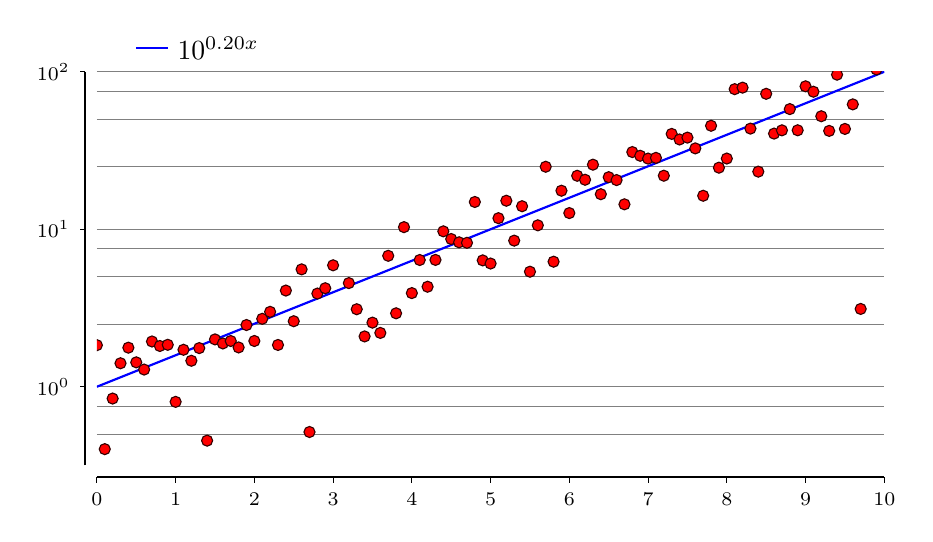
\begin{tikzpicture}
\begin{scope}[shift={(0.0,0.0)}]
\pgfsetxvec{\pgfpoint{1.0cm}{0cm}}
\pgfsetyvec{\pgfpoint{0cm}{2.0cm}}
\begin{scope}[shift={(0.0,0.5)}]
\begin{scope}[thick,black,fill=white]
\pgfpathmoveto{ \pgfpointadd{\pgfpointxy {0.0} {-0.5}} {\pgfpoint{0}{-0.15cm}} }
\pgfpathlineto{ \pgfpointadd{\pgfpointxy {10.0} {-0.5}} {\pgfpoint{0}{-0.15cm}} }
\pgfpathmoveto{ \pgfpointadd{\pgfpointxy {0.0} {-0.5}} {\pgfpoint{-0.15cm}{0}} }
\pgfpathlineto{ \pgfpointadd{\pgfpointxy {0.0} {2.0}} {\pgfpoint{-0.15cm}{0}} }
\pgfusepath{ stroke, }
\end{scope}
\begin{scope}[yshift=-0.15cm]
\draw[] [shift={(0.0,-0.5)}] (0,0) -- (0,-2pt) node[below]{ \scriptsize{\num[round-mode=places,round-precision=0]{0}}};
\draw[] [shift={(1.0,-0.5)}] (0,0) -- (0,-2pt) node[below]{ \scriptsize{\num[round-mode=places,round-precision=0]{1}}};
\draw[] [shift={(2.0,-0.5)}] (0,0) -- (0,-2pt) node[below]{ \scriptsize{\num[round-mode=places,round-precision=0]{2}}};
\draw[] [shift={(3.0,-0.5)}] (0,0) -- (0,-2pt) node[below]{ \scriptsize{\num[round-mode=places,round-precision=0]{3}}};
\draw[] [shift={(4.0,-0.5)}] (0,0) -- (0,-2pt) node[below]{ \scriptsize{\num[round-mode=places,round-precision=0]{4}}};
\draw[] [shift={(5.0,-0.5)}] (0,0) -- (0,-2pt) node[below]{ \scriptsize{\num[round-mode=places,round-precision=0]{5}}};
\draw[] [shift={(6.0,-0.5)}] (0,0) -- (0,-2pt) node[below]{ \scriptsize{\num[round-mode=places,round-precision=0]{6}}};
\draw[] [shift={(7.0,-0.5)}] (0,0) -- (0,-2pt) node[below]{ \scriptsize{\num[round-mode=places,round-precision=0]{7}}};
\draw[] [shift={(8.0,-0.5)}] (0,0) -- (0,-2pt) node[below]{ \scriptsize{\num[round-mode=places,round-precision=0]{8}}};
\draw[] [shift={(9.0,-0.5)}] (0,0) -- (0,-2pt) node[below]{ \scriptsize{\num[round-mode=places,round-precision=0]{9}}};
\draw[] [shift={(10.0,-0.5)}] (0,0) -- (0,-2pt) node[below]{ \scriptsize{\num[round-mode=places,round-precision=0]{10}}};
\end{scope}
\begin{scope}[xshift=-0.15cm]
\end{scope}
\end{scope}
\pgfsetxvec{\pgfpoint{1cm}{0cm}}
\pgfsetyvec{\pgfpoint{0cm}{1cm}}
\end{scope}
\begin{scope}[shift={(0.0,0.0)}]
\pgfsetxvec{\pgfpoint{1.0cm}{0cm}}
\pgfsetyvec{\pgfpoint{0cm}{2.0cm}}
\begin{scope}[shift={(0.0,0.5)}]
\begin{scope}[thin,gray]
\pgfpathmoveto{ \pgfpointxy {0.0} {-0.30102998}}
\pgfpathlineto{ \pgfpointxy {10.0} {-0.30102998}}
\pgfpathmoveto{ \pgfpointxy {0.0} {-0.12493874}}
\pgfpathlineto{ \pgfpointxy {10.0} {-0.12493874}}
\pgfpathmoveto{ \pgfpointxy {0.0} {0.0}}
\pgfpathlineto{ \pgfpointxy {10.0} {0.0}}
\pgfpathmoveto{ \pgfpointxy {0.0} {0.39794}}
\pgfpathlineto{ \pgfpointxy {10.0} {0.39794}}
\pgfpathmoveto{ \pgfpointxy {0.0} {0.69897}}
\pgfpathlineto{ \pgfpointxy {10.0} {0.69897}}
\pgfpathmoveto{ \pgfpointxy {0.0} {0.8750613}}
\pgfpathlineto{ \pgfpointxy {10.0} {0.8750613}}
\pgfpathmoveto{ \pgfpointxy {0.0} {1.0}}
\pgfpathlineto{ \pgfpointxy {10.0} {1.0}}
\pgfpathmoveto{ \pgfpointxy {0.0} {1.39794}}
\pgfpathlineto{ \pgfpointxy {10.0} {1.39794}}
\pgfpathmoveto{ \pgfpointxy {0.0} {1.69897}}
\pgfpathlineto{ \pgfpointxy {10.0} {1.69897}}
\pgfpathmoveto{ \pgfpointxy {0.0} {1.8750613}}
\pgfpathlineto{ \pgfpointxy {10.0} {1.8750613}}
\pgfpathmoveto{ \pgfpointxy {0.0} {2.0}}
\pgfpathlineto{ \pgfpointxy {10.0} {2.0}}
\pgfusepath{ stroke, }
\end{scope}
\end{scope}
\pgfsetxvec{\pgfpoint{1cm}{0cm}}
\pgfsetyvec{\pgfpoint{0cm}{1cm}}
\end{scope}
\begin{scope}[shift={(0.0,0.0)}]
\pgfsetxvec{\pgfpoint{1.0cm}{0cm}}
\pgfsetyvec{\pgfpoint{0cm}{2.0cm}}
\begin{scope}[shift={(0.0,0.5)}]
\begin{scope}[xshift=-0.15cm]
\draw[black] [shift={(0.0,0.0)}] (0,0) -- (-2pt,0) node[left]{ \scriptsize{$10^{0}$}};
\draw[black] [shift={(0.0,1.0)}] (0,0) -- (-2pt,0) node[left]{ \scriptsize{$10^{1}$}};
\draw[black] [shift={(0.0,2.0)}] (0,0) -- (-2pt,0) node[left]{ \scriptsize{$10^{2}$}};
\end{scope}
\end{scope}
\pgfsetxvec{\pgfpoint{1cm}{0cm}}
\pgfsetyvec{\pgfpoint{0cm}{1cm}}
\end{scope}
\begin{scope}[]
\pgfpathmoveto{ \pgfpointadd{\pgfpointxy {0.0} {0.0}} {\pgfpoint{0cm}{0cm}} }
\pgfpathlineto{ \pgfpointadd{\pgfpointxy {0.0} {0.0}} {\pgfpoint{10cm}{0cm}} }
\pgfpathlineto{ \pgfpointadd{\pgfpointxy {0.0} {0.0}} {\pgfpoint{10cm}{5cm}} }
\pgfpathlineto{ \pgfpointadd{\pgfpointxy {0.0} {0.0}} {\pgfpoint{0cm}{5cm}} }
\pgfpathclose
\pgfusepath{  clip, }
\begin{scope}[shift={(0.0,0.0)}]
\pgfsetxvec{\pgfpoint{1.0cm}{0cm}}
\pgfsetyvec{\pgfpoint{0cm}{2.0cm}}
\begin{scope}[shift={(0.0,0.5)}]
\begin{scope}[blue,thick]
\pgfpathmoveto{ \pgfpointxy {0.0} {0.0}}
\pgfpathlineto{ \pgfpointxy {0.1} {0.020000003}}
\pgfpathlineto{ \pgfpointxy {0.2} {0.04000001}}
\pgfpathlineto{ \pgfpointxy {0.3} {0.060000017}}
\pgfpathlineto{ \pgfpointxy {0.4} {0.08}}
\pgfpathlineto{ \pgfpointxy {0.5} {0.1}}
\pgfpathlineto{ \pgfpointxy {0.6} {0.12}}
\pgfpathlineto{ \pgfpointxy {0.7} {0.14000002}}
\pgfpathlineto{ \pgfpointxy {0.8} {0.16000001}}
\pgfpathlineto{ \pgfpointxy {0.9} {0.17999999}}
\pgfpathlineto{ \pgfpointxy {1.0} {0.2}}
\pgfpathlineto{ \pgfpointxy {1.1} {0.22}}
\pgfpathlineto{ \pgfpointxy {1.2} {0.24}}
\pgfpathlineto{ \pgfpointxy {1.3} {0.26}}
\pgfpathlineto{ \pgfpointxy {1.4} {0.28}}
\pgfpathlineto{ \pgfpointxy {1.5} {0.3}}
\pgfpathlineto{ \pgfpointxy {1.6} {0.32000002}}
\pgfpathlineto{ \pgfpointxy {1.7} {0.33999997}}
\pgfpathlineto{ \pgfpointxy {1.8} {0.35999998}}
\pgfpathlineto{ \pgfpointxy {1.9} {0.37999997}}
\pgfpathlineto{ \pgfpointxy {2.0} {0.39999998}}
\pgfpathlineto{ \pgfpointxy {2.1} {0.41999996}}
\pgfpathlineto{ \pgfpointxy {2.2} {0.44}}
\pgfpathlineto{ \pgfpointxy {2.3} {0.46}}
\pgfpathlineto{ \pgfpointxy {2.4} {0.48}}
\pgfpathlineto{ \pgfpointxy {2.5} {0.5}}
\pgfpathlineto{ \pgfpointxy {2.6} {0.52}}
\pgfpathlineto{ \pgfpointxy {2.7} {0.53999996}}
\pgfpathlineto{ \pgfpointxy {2.8} {0.56}}
\pgfpathlineto{ \pgfpointxy {2.9} {0.58000004}}
\pgfpathlineto{ \pgfpointxy {3.0} {0.6}}
\pgfpathlineto{ \pgfpointxy {3.1} {0.62}}
\pgfpathlineto{ \pgfpointxy {3.2} {0.64}}
\pgfpathlineto{ \pgfpointxy {3.3} {0.66}}
\pgfpathlineto{ \pgfpointxy {3.4} {0.68}}
\pgfpathlineto{ \pgfpointxy {3.5} {0.7}}
\pgfpathlineto{ \pgfpointxy {3.6} {0.7199999}}
\pgfpathlineto{ \pgfpointxy {3.7} {0.74}}
\pgfpathlineto{ \pgfpointxy {3.8} {0.76}}
\pgfpathlineto{ \pgfpointxy {3.9} {0.78000003}}
\pgfpathlineto{ \pgfpointxy {4.0} {0.8}}
\pgfpathlineto{ \pgfpointxy {4.1} {0.82}}
\pgfpathlineto{ \pgfpointxy {4.2} {0.84}}
\pgfpathlineto{ \pgfpointxy {4.3} {0.8600001}}
\pgfpathlineto{ \pgfpointxy {4.4} {0.88}}
\pgfpathlineto{ \pgfpointxy {4.5} {0.90000004}}
\pgfpathlineto{ \pgfpointxy {4.6} {0.92}}
\pgfpathlineto{ \pgfpointxy {4.7} {0.93999994}}
\pgfpathlineto{ \pgfpointxy {4.8} {0.9600001}}
\pgfpathlineto{ \pgfpointxy {4.9} {0.97999996}}
\pgfpathlineto{ \pgfpointxy {5.0} {1.0}}
\pgfpathlineto{ \pgfpointxy {5.1} {1.0199999}}
\pgfpathlineto{ \pgfpointxy {5.2} {1.04}}
\pgfpathlineto{ \pgfpointxy {5.3} {1.0600001}}
\pgfpathlineto{ \pgfpointxy {5.4} {1.08}}
\pgfpathlineto{ \pgfpointxy {5.5} {1.1}}
\pgfpathlineto{ \pgfpointxy {5.6} {1.12}}
\pgfpathlineto{ \pgfpointxy {5.7} {1.14}}
\pgfpathlineto{ \pgfpointxy {5.8} {1.1600001}}
\pgfpathlineto{ \pgfpointxy {5.9} {1.1800001}}
\pgfpathlineto{ \pgfpointxy {6.0} {1.2}}
\pgfpathlineto{ \pgfpointxy {6.1} {1.22}}
\pgfpathlineto{ \pgfpointxy {6.2} {1.24}}
\pgfpathlineto{ \pgfpointxy {6.3} {1.2600001}}
\pgfpathlineto{ \pgfpointxy {6.4} {1.28}}
\pgfpathlineto{ \pgfpointxy {6.5} {1.3000001}}
\pgfpathlineto{ \pgfpointxy {6.6} {1.32}}
\pgfpathlineto{ \pgfpointxy {6.7} {1.34}}
\pgfpathlineto{ \pgfpointxy {6.8} {1.36}}
\pgfpathlineto{ \pgfpointxy {6.9} {1.38}}
\pgfpathlineto{ \pgfpointxy {7.0} {1.4}}
\pgfpathlineto{ \pgfpointxy {7.1} {1.42}}
\pgfpathlineto{ \pgfpointxy {7.2} {1.4399999}}
\pgfpathlineto{ \pgfpointxy {7.3} {1.4599999}}
\pgfpathlineto{ \pgfpointxy {7.4} {1.48}}
\pgfpathlineto{ \pgfpointxy {7.5} {1.5}}
\pgfpathlineto{ \pgfpointxy {7.6} {1.5199999}}
\pgfpathlineto{ \pgfpointxy {7.7} {1.54}}
\pgfpathlineto{ \pgfpointxy {7.8} {1.5600001}}
\pgfpathlineto{ \pgfpointxy {7.9} {1.58}}
\pgfpathlineto{ \pgfpointxy {8.0} {1.6}}
\pgfpathlineto{ \pgfpointxy {8.1} {1.6200001}}
\pgfpathlineto{ \pgfpointxy {8.2} {1.6399999}}
\pgfpathlineto{ \pgfpointxy {8.3} {1.6600001}}
\pgfpathlineto{ \pgfpointxy {8.4} {1.68}}
\pgfpathlineto{ \pgfpointxy {8.5} {1.7}}
\pgfpathlineto{ \pgfpointxy {8.6} {1.72}}
\pgfpathlineto{ \pgfpointxy {8.7} {1.7400001}}
\pgfpathlineto{ \pgfpointxy {8.8} {1.76}}
\pgfpathlineto{ \pgfpointxy {8.9} {1.78}}
\pgfpathlineto{ \pgfpointxy {9.0} {1.8000001}}
\pgfpathlineto{ \pgfpointxy {9.1} {1.8199999}}
\pgfpathlineto{ \pgfpointxy {9.2} {1.84}}
\pgfpathlineto{ \pgfpointxy {9.3} {1.86}}
\pgfpathlineto{ \pgfpointxy {9.4} {1.8799999}}
\pgfpathlineto{ \pgfpointxy {9.5} {1.9}}
\pgfpathlineto{ \pgfpointxy {9.6} {1.9200002}}
\pgfpathlineto{ \pgfpointxy {9.7} {1.9399998}}
\pgfpathlineto{ \pgfpointxy {9.8} {1.9599999}}
\pgfpathlineto{ \pgfpointxy {9.9} {1.9799999}}
\pgfpathlineto{ \pgfpointxy {10.0} {2.0}}
\pgfusepath{ stroke, }
\end{scope}
\end{scope}
\pgfsetxvec{\pgfpoint{1cm}{0cm}}
\pgfsetyvec{\pgfpoint{0cm}{1cm}}
\end{scope}
\end{scope}
\draw[blue,thick] (0.5,5.3) -- (0.9,5.3);
\node at (0.9,5.3) [right,,] {$10^{0.20 x}$};
\begin{scope}[]
\pgfpathmoveto{ \pgfpointadd{\pgfpointxy {0.0} {0.0}} {\pgfpoint{0cm}{0cm}} }
\pgfpathlineto{ \pgfpointadd{\pgfpointxy {0.0} {0.0}} {\pgfpoint{10cm}{0cm}} }
\pgfpathlineto{ \pgfpointadd{\pgfpointxy {0.0} {0.0}} {\pgfpoint{10cm}{5cm}} }
\pgfpathlineto{ \pgfpointadd{\pgfpointxy {0.0} {0.0}} {\pgfpoint{0cm}{5cm}} }
\pgfpathclose
\pgfusepath{  clip, }
\begin{scope}[shift={(0.0,0.0)}]
\pgfsetxvec{\pgfpoint{1.0cm}{0cm}}
\pgfsetyvec{\pgfpoint{0cm}{2.0cm}}
\begin{scope}[shift={(0.0,0.5)}]
\node at (0.0,0.26394337985485333) [fill=red,draw=red!20!black,circle,inner sep=0.0pt,minimum width =4.0pt,minimum height=4.0pt] {};
\node at (0.1,-0.3961832630965618) [fill=red,draw=red!20!black,circle,inner sep=0.0pt,minimum width =4.0pt,minimum height=4.0pt] {};
\node at (0.2,-0.07486858598533142) [fill=red,draw=red!20!black,circle,inner sep=0.0pt,minimum width =4.0pt,minimum height=4.0pt] {};
\node at (0.3,0.14920116021563481) [fill=red,draw=red!20!black,circle,inner sep=0.0pt,minimum width =4.0pt,minimum height=4.0pt] {};
\node at (0.4,0.2481192749940075) [fill=red,draw=red!20!black,circle,inner sep=0.0pt,minimum width =4.0pt,minimum height=4.0pt] {};
\node at (0.5,0.15493185738567844) [fill=red,draw=red!20!black,circle,inner sep=0.0pt,minimum width =4.0pt,minimum height=4.0pt] {};
\node at (0.6,0.10917378912034231) [fill=red,draw=red!20!black,circle,inner sep=0.0pt,minimum width =4.0pt,minimum height=4.0pt] {};
\node at (0.7,0.28742310524644665) [fill=red,draw=red!20!black,circle,inner sep=0.0pt,minimum width =4.0pt,minimum height=4.0pt] {};
\node at (0.8,0.25882215084447646) [fill=red,draw=red!20!black,circle,inner sep=0.0pt,minimum width =4.0pt,minimum height=4.0pt] {};
\node at (0.90000004,0.2664258892116321) [fill=red,draw=red!20!black,circle,inner sep=0.0pt,minimum width =4.0pt,minimum height=4.0pt] {};
\node at (1.0,-0.09602285995554843) [fill=red,draw=red!20!black,circle,inner sep=0.0pt,minimum width =4.0pt,minimum height=4.0pt] {};
\node at (1.1,0.23474145100891797) [fill=red,draw=red!20!black,circle,inner sep=0.0pt,minimum width =4.0pt,minimum height=4.0pt] {};
\node at (1.2,0.1649517845055302) [fill=red,draw=red!20!black,circle,inner sep=0.0pt,minimum width =4.0pt,minimum height=4.0pt] {};
\node at (1.3000001,0.24541415947577902) [fill=red,draw=red!20!black,circle,inner sep=0.0pt,minimum width =4.0pt,minimum height=4.0pt] {};
\node at (1.4,-0.342178597467006) [fill=red,draw=red!20!black,circle,inner sep=0.0pt,minimum width =4.0pt,minimum height=4.0pt] {};
\node at (1.5,0.30072677470093273) [fill=red,draw=red!20!black,circle,inner sep=0.0pt,minimum width =4.0pt,minimum height=4.0pt] {};
\node at (1.6,0.27498400753166763) [fill=red,draw=red!20!black,circle,inner sep=0.0pt,minimum width =4.0pt,minimum height=4.0pt] {};
\node at (1.7,0.29035905162508957) [fill=red,draw=red!20!black,circle,inner sep=0.0pt,minimum width =4.0pt,minimum height=4.0pt] {};
\node at (1.8000001,0.24963323707735238) [fill=red,draw=red!20!black,circle,inner sep=0.0pt,minimum width =4.0pt,minimum height=4.0pt] {};
\node at (1.9,0.39187057265016695) [fill=red,draw=red!20!black,circle,inner sep=0.0pt,minimum width =4.0pt,minimum height=4.0pt] {};
\node at (2.0,0.2904804231890059) [fill=red,draw=red!20!black,circle,inner sep=0.0pt,minimum width =4.0pt,minimum height=4.0pt] {};
\node at (2.1000001,0.4313654986378826) [fill=red,draw=red!20!black,circle,inner sep=0.0pt,minimum width =4.0pt,minimum height=4.0pt] {};
\node at (2.2,0.4756632777991412) [fill=red,draw=red!20!black,circle,inner sep=0.0pt,minimum width =4.0pt,minimum height=4.0pt] {};
\node at (2.3,0.265296108015851) [fill=red,draw=red!20!black,circle,inner sep=0.0pt,minimum width =4.0pt,minimum height=4.0pt] {};
\node at (2.4,0.6108197514323496) [fill=red,draw=red!20!black,circle,inner sep=0.0pt,minimum width =4.0pt,minimum height=4.0pt] {};
\node at (2.5,0.4160372308334822) [fill=red,draw=red!20!black,circle,inner sep=0.0pt,minimum width =4.0pt,minimum height=4.0pt] {};
\node at (2.6000001,0.7454294326953202) [fill=red,draw=red!20!black,circle,inner sep=0.0pt,minimum width =4.0pt,minimum height=4.0pt] {};
\node at (2.7,-0.28734829605883166) [fill=red,draw=red!20!black,circle,inner sep=0.0pt,minimum width =4.0pt,minimum height=4.0pt] {};
\node at (2.8,0.5916655990149627) [fill=red,draw=red!20!black,circle,inner sep=0.0pt,minimum width =4.0pt,minimum height=4.0pt] {};
\node at (2.9,0.6255529660072152) [fill=red,draw=red!20!black,circle,inner sep=0.0pt,minimum width =4.0pt,minimum height=4.0pt] {};
\node at (3.0,0.7712121207760849) [fill=red,draw=red!20!black,circle,inner sep=0.0pt,minimum width =4.0pt,minimum height=4.0pt] {};
\node at (3.1000001,-2.0) [fill=red,draw=red!20!black,circle,inner sep=0.0pt,minimum width =4.0pt,minimum height=4.0pt] {};
\node at (3.2,0.6582745916421413) [fill=red,draw=red!20!black,circle,inner sep=0.0pt,minimum width =4.0pt,minimum height=4.0pt] {};
\node at (3.3,0.49218878008893274) [fill=red,draw=red!20!black,circle,inner sep=0.0pt,minimum width =4.0pt,minimum height=4.0pt] {};
\node at (3.4,0.3195132866057407) [fill=red,draw=red!20!black,circle,inner sep=0.0pt,minimum width =4.0pt,minimum height=4.0pt] {};
\node at (3.5,0.40708641630439074) [fill=red,draw=red!20!black,circle,inner sep=0.0pt,minimum width =4.0pt,minimum height=4.0pt] {};
\node at (3.6000001,0.34178586215238793) [fill=red,draw=red!20!black,circle,inner sep=0.0pt,minimum width =4.0pt,minimum height=4.0pt] {};
\node at (3.7,0.8314527836447386) [fill=red,draw=red!20!black,circle,inner sep=0.0pt,minimum width =4.0pt,minimum height=4.0pt] {};
\node at (3.8,0.46634991669308007) [fill=red,draw=red!20!black,circle,inner sep=0.0pt,minimum width =4.0pt,minimum height=4.0pt] {};
\node at (3.9,1.013451826648603) [fill=red,draw=red!20!black,circle,inner sep=0.0pt,minimum width =4.0pt,minimum height=4.0pt] {};
\node at (4.0,0.5946616294943309) [fill=red,draw=red!20!black,circle,inner sep=0.0pt,minimum width =4.0pt,minimum height=4.0pt] {};
\node at (4.1,0.8047758610140427) [fill=red,draw=red!20!black,circle,inner sep=0.0pt,minimum width =4.0pt,minimum height=4.0pt] {};
\node at (4.2000003,0.6350342955122901) [fill=red,draw=red!20!black,circle,inner sep=0.0pt,minimum width =4.0pt,minimum height=4.0pt] {};
\node at (4.3,0.805442171005536) [fill=red,draw=red!20!black,circle,inner sep=0.0pt,minimum width =4.0pt,minimum height=4.0pt] {};
\node at (4.4,0.9868170043628214) [fill=red,draw=red!20!black,circle,inner sep=0.0pt,minimum width =4.0pt,minimum height=4.0pt] {};
\node at (4.5,0.9379910652499258) [fill=red,draw=red!20!black,circle,inner sep=0.0pt,minimum width =4.0pt,minimum height=4.0pt] {};
\node at (4.6,0.9172382039601246) [fill=red,draw=red!20!black,circle,inner sep=0.0pt,minimum width =4.0pt,minimum height=4.0pt] {};
\node at (4.7000003,0.9139332301471813) [fill=red,draw=red!20!black,circle,inner sep=0.0pt,minimum width =4.0pt,minimum height=4.0pt] {};
\node at (4.8,1.1732196713222418) [fill=red,draw=red!20!black,circle,inner sep=0.0pt,minimum width =4.0pt,minimum height=4.0pt] {};
\node at (4.9,0.8023915034932178) [fill=red,draw=red!20!black,circle,inner sep=0.0pt,minimum width =4.0pt,minimum height=4.0pt] {};
\node at (5.0,0.7824377391285007) [fill=red,draw=red!20!black,circle,inner sep=0.0pt,minimum width =4.0pt,minimum height=4.0pt] {};
\node at (5.1,1.0703008248499204) [fill=red,draw=red!20!black,circle,inner sep=0.0pt,minimum width =4.0pt,minimum height=4.0pt] {};
\node at (5.2000003,1.1811804507027164) [fill=red,draw=red!20!black,circle,inner sep=0.0pt,minimum width =4.0pt,minimum height=4.0pt] {};
\node at (5.3,0.9277563645992261) [fill=red,draw=red!20!black,circle,inner sep=0.0pt,minimum width =4.0pt,minimum height=4.0pt] {};
\node at (5.4,1.146299362106598) [fill=red,draw=red!20!black,circle,inner sep=0.0pt,minimum width =4.0pt,minimum height=4.0pt] {};
\node at (5.5,0.7305039985297197) [fill=red,draw=red!20!black,circle,inner sep=0.0pt,minimum width =4.0pt,minimum height=4.0pt] {};
\node at (5.6,1.0249977123623562) [fill=red,draw=red!20!black,circle,inner sep=0.0pt,minimum width =4.0pt,minimum height=4.0pt] {};
\node at (5.7000003,1.396912947693521) [fill=red,draw=red!20!black,circle,inner sep=0.0pt,minimum width =4.0pt,minimum height=4.0pt] {};
\node at (5.8,0.7941003361025282) [fill=red,draw=red!20!black,circle,inner sep=0.0pt,minimum width =4.0pt,minimum height=4.0pt] {};
\node at (5.9,1.2447777467435583) [fill=red,draw=red!20!black,circle,inner sep=0.0pt,minimum width =4.0pt,minimum height=4.0pt] {};
\node at (6.0,1.1027677569527998) [fill=red,draw=red!20!black,circle,inner sep=0.0pt,minimum width =4.0pt,minimum height=4.0pt] {};
\node at (6.1,1.3396655159606197) [fill=red,draw=red!20!black,circle,inner sep=0.0pt,minimum width =4.0pt,minimum height=4.0pt] {};
\node at (6.2000003,1.3142698592261517) [fill=red,draw=red!20!black,circle,inner sep=0.0pt,minimum width =4.0pt,minimum height=4.0pt] {};
\node at (6.3,1.410157339474974) [fill=red,draw=red!20!black,circle,inner sep=0.0pt,minimum width =4.0pt,minimum height=4.0pt] {};
\node at (6.4,1.2226390068367032) [fill=red,draw=red!20!black,circle,inner sep=0.0pt,minimum width =4.0pt,minimum height=4.0pt] {};
\node at (6.5,1.3306143061604019) [fill=red,draw=red!20!black,circle,inner sep=0.0pt,minimum width =4.0pt,minimum height=4.0pt] {};
\node at (6.6,1.3123449240208265) [fill=red,draw=red!20!black,circle,inner sep=0.0pt,minimum width =4.0pt,minimum height=4.0pt] {};
\node at (6.7000003,1.1584516153768685) [fill=red,draw=red!20!black,circle,inner sep=0.0pt,minimum width =4.0pt,minimum height=4.0pt] {};
\node at (6.8,1.4902204608617633) [fill=red,draw=red!20!black,circle,inner sep=0.0pt,minimum width =4.0pt,minimum height=4.0pt] {};
\node at (6.9,1.46662746541778) [fill=red,draw=red!20!black,circle,inner sep=0.0pt,minimum width =4.0pt,minimum height=4.0pt] {};
\node at (7.0,1.4486687195933237) [fill=red,draw=red!20!black,circle,inner sep=0.0pt,minimum width =4.0pt,minimum height=4.0pt] {};
\node at (7.1,1.45340144261818) [fill=red,draw=red!20!black,circle,inner sep=0.0pt,minimum width =4.0pt,minimum height=4.0pt] {};
\node at (7.2000003,1.3400286683942473) [fill=red,draw=red!20!black,circle,inner sep=0.0pt,minimum width =4.0pt,minimum height=4.0pt] {};
\node at (7.3,1.6055162689945728) [fill=red,draw=red!20!black,circle,inner sep=0.0pt,minimum width =4.0pt,minimum height=4.0pt] {};
\node at (7.4,1.570074004938375) [fill=red,draw=red!20!black,circle,inner sep=0.0pt,minimum width =4.0pt,minimum height=4.0pt] {};
\node at (7.5,1.581943908908274) [fill=red,draw=red!20!black,circle,inner sep=0.0pt,minimum width =4.0pt,minimum height=4.0pt] {};
\node at (7.6,1.513525885072603) [fill=red,draw=red!20!black,circle,inner sep=0.0pt,minimum width =4.0pt,minimum height=4.0pt] {};
\node at (7.7000003,1.212805233919764) [fill=red,draw=red!20!black,circle,inner sep=0.0pt,minimum width =4.0pt,minimum height=4.0pt] {};
\node at (7.8,1.6572107079224174) [fill=red,draw=red!20!black,circle,inner sep=0.0pt,minimum width =4.0pt,minimum height=4.0pt] {};
\node at (7.9,1.3910689520925066) [fill=red,draw=red!20!black,circle,inner sep=0.0pt,minimum width =4.0pt,minimum height=4.0pt] {};
\node at (8.0,1.4490153248036504) [fill=red,draw=red!20!black,circle,inner sep=0.0pt,minimum width =4.0pt,minimum height=4.0pt] {};
\node at (8.1,1.8896836488137665) [fill=red,draw=red!20!black,circle,inner sep=0.0pt,minimum width =4.0pt,minimum height=4.0pt] {};
\node at (8.2,1.899311906078869) [fill=red,draw=red!20!black,circle,inner sep=0.0pt,minimum width =4.0pt,minimum height=4.0pt] {};
\node at (8.3,1.6391310472548593) [fill=red,draw=red!20!black,circle,inner sep=0.0pt,minimum width =4.0pt,minimum height=4.0pt] {};
\node at (8.400001,1.3658200900813722) [fill=red,draw=red!20!black,circle,inner sep=0.0pt,minimum width =4.0pt,minimum height=4.0pt] {};
\node at (8.5,1.8601600049499194) [fill=red,draw=red!20!black,circle,inner sep=0.0pt,minimum width =4.0pt,minimum height=4.0pt] {};
\node at (8.6,1.607452314720941) [fill=red,draw=red!20!black,circle,inner sep=0.0pt,minimum width =4.0pt,minimum height=4.0pt] {};
\node at (8.7,1.6282183481909387) [fill=red,draw=red!20!black,circle,inner sep=0.0pt,minimum width =4.0pt,minimum height=4.0pt] {};
\node at (8.8,1.7630718478643668) [fill=red,draw=red!20!black,circle,inner sep=0.0pt,minimum width =4.0pt,minimum height=4.0pt] {};
\node at (8.900001,1.6285183644793773) [fill=red,draw=red!20!black,circle,inner sep=0.0pt,minimum width =4.0pt,minimum height=4.0pt] {};
\node at (9.0,1.9077529445730141) [fill=red,draw=red!20!black,circle,inner sep=0.0pt,minimum width =4.0pt,minimum height=4.0pt] {};
\node at (9.1,1.8732645874639682) [fill=red,draw=red!20!black,circle,inner sep=0.0pt,minimum width =4.0pt,minimum height=4.0pt] {};
\node at (9.2,1.7175941929643084) [fill=red,draw=red!20!black,circle,inner sep=0.0pt,minimum width =4.0pt,minimum height=4.0pt] {};
\node at (9.3,1.6246193627573036) [fill=red,draw=red!20!black,circle,inner sep=0.0pt,minimum width =4.0pt,minimum height=4.0pt] {};
\node at (9.400001,1.981626977873689) [fill=red,draw=red!20!black,circle,inner sep=0.0pt,minimum width =4.0pt,minimum height=4.0pt] {};
\node at (9.5,1.63708736984028) [fill=red,draw=red!20!black,circle,inner sep=0.0pt,minimum width =4.0pt,minimum height=4.0pt] {};
\node at (9.6,1.7930615036688613) [fill=red,draw=red!20!black,circle,inner sep=0.0pt,minimum width =4.0pt,minimum height=4.0pt] {};
\node at (9.7,0.49408047318778076) [fill=red,draw=red!20!black,circle,inner sep=0.0pt,minimum width =4.0pt,minimum height=4.0pt] {};
\node at (9.8,2.2056921710355915) [fill=red,draw=red!20!black,circle,inner sep=0.0pt,minimum width =4.0pt,minimum height=4.0pt] {};
\node at (9.900001,2.014790351067405) [fill=red,draw=red!20!black,circle,inner sep=0.0pt,minimum width =4.0pt,minimum height=4.0pt] {};
\node at (10.0,2.2032156407842334) [fill=red,draw=red!20!black,circle,inner sep=0.0pt,minimum width =4.0pt,minimum height=4.0pt] {};
\end{scope}
\pgfsetxvec{\pgfpoint{1cm}{0cm}}
\pgfsetyvec{\pgfpoint{0cm}{1cm}}
\end{scope}
\end{scope}
\end{tikzpicture}
\end{document}

\captionsetup{singlelinecheck=off}
\caption[asdf]{Plot with log scale in the y direction. Explicit transformation.}
\end{figure}
\section{2D histograms}


2D representations of 2D histograms.

\begin{figure}[H]
\centering
\documentclass{standalone}
\ifx\HCode\UnDef\else\def\pgfsysdriver{pgfsys-tex4ht.def}\fi
\usepackage[usenames,dvipsnames,svgnames,table]{xcolor}
\usepackage{tikz}
\usepackage{color}
\usepackage{siunitx}
\usetikzlibrary{arrows,shapes}
\begin{document}
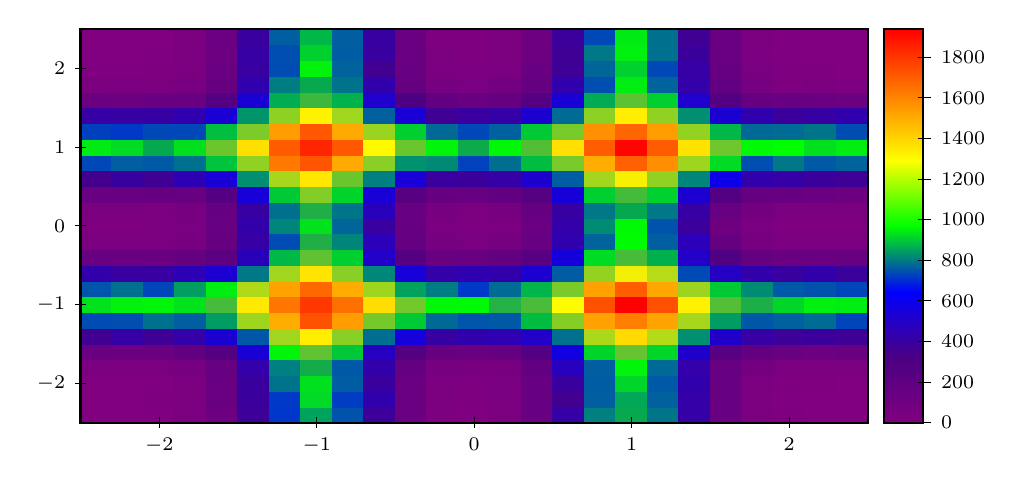
\begin{tikzpicture}
\begin{scope}[]
\pgfpointadd{\pgfpointxy {0.0} {0.0}} {\pgfpoint{0cm}{0cm}}\pgfpathmoveto{ NIL }
\pgfpointadd{\pgfpointxy {0.0} {0.0}} {\pgfpoint{10cm}{0cm}}\pgfpathlineto{ NIL }
\pgfpointadd{\pgfpointxy {0.0} {0.0}} {\pgfpoint{10cm}{5cm}}\pgfpathlineto{ NIL }
\pgfpointadd{\pgfpointxy {0.0} {0.0}} {\pgfpoint{0cm}{5cm}}\pgfpathlineto{ NIL }
\pgfpathclose
\pgfusepath{  clip, }
\begin{scope}[shift={(0.0,0.0)}]
\pgfsetxvec{\pgfpoint{2.0cm}{0cm}}
\pgfsetyvec{\pgfpoint{0cm}{1.0cm}}
\begin{scope}[shift={(2.5,2.5)}]
\begin{scope}[Indigo!0!violet]
\pgfpathmoveto{ \pgfpointxy {-2.5} {-2.5}}
\pgfpathlineto{ \pgfpointxy {-2.3} {-2.5}}
\pgfpathlineto{ \pgfpointxy {-2.3} {-2.3}}
\pgfpathlineto{ \pgfpointxy {-2.5} {-2.3}}
\pgfpathclose
\pgfusepath{ stroke, fill, }
\end{scope}
\begin{scope}[Indigo!0!violet]
\pgfpathmoveto{ \pgfpointxy {-2.3} {-2.5}}
\pgfpathlineto{ \pgfpointxy {-2.1} {-2.5}}
\pgfpathlineto{ \pgfpointxy {-2.1} {-2.3}}
\pgfpathlineto{ \pgfpointxy {-2.3} {-2.3}}
\pgfpathclose
\pgfusepath{ stroke, fill, }
\end{scope}
\begin{scope}[Indigo!1!violet]
\pgfpathmoveto{ \pgfpointxy {-2.1} {-2.5}}
\pgfpathlineto{ \pgfpointxy {-1.8999999} {-2.5}}
\pgfpathlineto{ \pgfpointxy {-1.8999999} {-2.3}}
\pgfpathlineto{ \pgfpointxy {-2.1} {-2.3}}
\pgfpathclose
\pgfusepath{ stroke, fill, }
\end{scope}
\begin{scope}[Indigo!11!violet]
\pgfpathmoveto{ \pgfpointxy {-1.9} {-2.5}}
\pgfpathlineto{ \pgfpointxy {-1.6999999} {-2.5}}
\pgfpathlineto{ \pgfpointxy {-1.6999999} {-2.3}}
\pgfpathlineto{ \pgfpointxy {-1.9} {-2.3}}
\pgfpathclose
\pgfusepath{ stroke, fill, }
\end{scope}
\begin{scope}[Indigo!38!violet]
\pgfpathmoveto{ \pgfpointxy {-1.7} {-2.5}}
\pgfpathlineto{ \pgfpointxy {-1.5} {-2.5}}
\pgfpathlineto{ \pgfpointxy {-1.5} {-2.3}}
\pgfpathlineto{ \pgfpointxy {-1.7} {-2.3}}
\pgfpathclose
\pgfusepath{ stroke, fill, }
\end{scope}
\begin{scope}[blue!18!Indigo]
\pgfpathmoveto{ \pgfpointxy {-1.5} {-2.5}}
\pgfpathlineto{ \pgfpointxy {-1.3} {-2.5}}
\pgfpathlineto{ \pgfpointxy {-1.3} {-2.3}}
\pgfpathlineto{ \pgfpointxy {-1.5} {-2.3}}
\pgfpathclose
\pgfusepath{ stroke, fill, }
\end{scope}
\begin{scope}[green!21!blue]
\pgfpathmoveto{ \pgfpointxy {-1.3} {-2.5}}
\pgfpathlineto{ \pgfpointxy {-1.0999999} {-2.5}}
\pgfpathlineto{ \pgfpointxy {-1.0999999} {-2.3}}
\pgfpathlineto{ \pgfpointxy {-1.3} {-2.3}}
\pgfpathclose
\pgfusepath{ stroke, fill, }
\end{scope}
\begin{scope}[green!64!blue]
\pgfpathmoveto{ \pgfpointxy {-1.1} {-2.5}}
\pgfpathlineto{ \pgfpointxy {-0.90000004} {-2.5}}
\pgfpathlineto{ \pgfpointxy {-0.90000004} {-2.3}}
\pgfpathlineto{ \pgfpointxy {-1.1} {-2.3}}
\pgfpathclose
\pgfusepath{ stroke, fill, }
\end{scope}
\begin{scope}[green!32!blue]
\pgfpathmoveto{ \pgfpointxy {-0.9} {-2.5}}
\pgfpathlineto{ \pgfpointxy {-0.7} {-2.5}}
\pgfpathlineto{ \pgfpointxy {-0.7} {-2.3}}
\pgfpathlineto{ \pgfpointxy {-0.9} {-2.3}}
\pgfpathclose
\pgfusepath{ stroke, fill, }
\end{scope}
\begin{scope}[blue!19!Indigo]
\pgfpathmoveto{ \pgfpointxy {-0.6999999} {-2.5}}
\pgfpathlineto{ \pgfpointxy {-0.49999994} {-2.5}}
\pgfpathlineto{ \pgfpointxy {-0.49999994} {-2.3}}
\pgfpathlineto{ \pgfpointxy {-0.6999999} {-2.3}}
\pgfpathclose
\pgfusepath{ stroke, fill, }
\end{scope}
\begin{scope}[Indigo!40!violet]
\pgfpathmoveto{ \pgfpointxy {-0.5} {-2.5}}
\pgfpathlineto{ \pgfpointxy {-0.3} {-2.5}}
\pgfpathlineto{ \pgfpointxy {-0.3} {-2.3}}
\pgfpathlineto{ \pgfpointxy {-0.5} {-2.3}}
\pgfpathclose
\pgfusepath{ stroke, fill, }
\end{scope}
\begin{scope}[Indigo!7!violet]
\pgfpathmoveto{ \pgfpointxy {-0.29999995} {-2.5}}
\pgfpathlineto{ \pgfpointxy {-0.09999995} {-2.5}}
\pgfpathlineto{ \pgfpointxy {-0.09999995} {-2.3}}
\pgfpathlineto{ \pgfpointxy {-0.29999995} {-2.3}}
\pgfpathclose
\pgfusepath{ stroke, fill, }
\end{scope}
\begin{scope}[Indigo!1!violet]
\pgfpathmoveto{ \pgfpointxy {-0.099999905} {-2.5}}
\pgfpathlineto{ \pgfpointxy {0.1000001} {-2.5}}
\pgfpathlineto{ \pgfpointxy {0.1000001} {-2.3}}
\pgfpathlineto{ \pgfpointxy {-0.099999905} {-2.3}}
\pgfpathclose
\pgfusepath{ stroke, fill, }
\end{scope}
\begin{scope}[Indigo!10!violet]
\pgfpathmoveto{ \pgfpointxy {0.10000014} {-2.5}}
\pgfpathlineto{ \pgfpointxy {0.30000013} {-2.5}}
\pgfpathlineto{ \pgfpointxy {0.30000013} {-2.3}}
\pgfpathlineto{ \pgfpointxy {0.10000014} {-2.3}}
\pgfpathclose
\pgfusepath{ stroke, fill, }
\end{scope}
\begin{scope}[Indigo!42!violet]
\pgfpathmoveto{ \pgfpointxy {0.29999995} {-2.5}}
\pgfpathlineto{ \pgfpointxy {0.49999994} {-2.5}}
\pgfpathlineto{ \pgfpointxy {0.49999994} {-2.3}}
\pgfpathlineto{ \pgfpointxy {0.29999995} {-2.3}}
\pgfpathclose
\pgfusepath{ stroke, fill, }
\end{scope}
\begin{scope}[blue!29!Indigo]
\pgfpathmoveto{ \pgfpointxy {0.5} {-2.5}}
\pgfpathlineto{ \pgfpointxy {0.7} {-2.5}}
\pgfpathlineto{ \pgfpointxy {0.7} {-2.3}}
\pgfpathlineto{ \pgfpointxy {0.5} {-2.3}}
\pgfpathclose
\pgfusepath{ stroke, fill, }
\end{scope}
\begin{scope}[green!50!blue]
\pgfpathmoveto{ \pgfpointxy {0.70000005} {-2.5}}
\pgfpathlineto{ \pgfpointxy {0.90000004} {-2.5}}
\pgfpathlineto{ \pgfpointxy {0.90000004} {-2.3}}
\pgfpathlineto{ \pgfpointxy {0.70000005} {-2.3}}
\pgfpathclose
\pgfusepath{ stroke, fill, }
\end{scope}
\begin{scope}[yellow!3!green]
\pgfpathmoveto{ \pgfpointxy {0.9000001} {-2.5}}
\pgfpathlineto{ \pgfpointxy {1.1000001} {-2.5}}
\pgfpathlineto{ \pgfpointxy {1.1000001} {-2.3}}
\pgfpathlineto{ \pgfpointxy {0.9000001} {-2.3}}
\pgfpathclose
\pgfusepath{ stroke, fill, }
\end{scope}
\begin{scope}[green!46!blue]
\pgfpathmoveto{ \pgfpointxy {1.1000001} {-2.5}}
\pgfpathlineto{ \pgfpointxy {1.3000002} {-2.5}}
\pgfpathlineto{ \pgfpointxy {1.3000002} {-2.3}}
\pgfpathlineto{ \pgfpointxy {1.1000001} {-2.3}}
\pgfpathclose
\pgfusepath{ stroke, fill, }
\end{scope}
\begin{scope}[blue!29!Indigo]
\pgfpathmoveto{ \pgfpointxy {1.3} {-2.5}}
\pgfpathlineto{ \pgfpointxy {1.5} {-2.5}}
\pgfpathlineto{ \pgfpointxy {1.5} {-2.3}}
\pgfpathlineto{ \pgfpointxy {1.3} {-2.3}}
\pgfpathclose
\pgfusepath{ stroke, fill, }
\end{scope}
\begin{scope}[Indigo!44!violet]
\pgfpathmoveto{ \pgfpointxy {1.5} {-2.5}}
\pgfpathlineto{ \pgfpointxy {1.7} {-2.5}}
\pgfpathlineto{ \pgfpointxy {1.7} {-2.3}}
\pgfpathlineto{ \pgfpointxy {1.5} {-2.3}}
\pgfpathclose
\pgfusepath{ stroke, fill, }
\end{scope}
\begin{scope}[Indigo!10!violet]
\pgfpathmoveto{ \pgfpointxy {1.7000003} {-2.5}}
\pgfpathlineto{ \pgfpointxy {1.9000003} {-2.5}}
\pgfpathlineto{ \pgfpointxy {1.9000003} {-2.3}}
\pgfpathlineto{ \pgfpointxy {1.7000003} {-2.3}}
\pgfpathclose
\pgfusepath{ stroke, fill, }
\end{scope}
\begin{scope}[Indigo!2!violet]
\pgfpathmoveto{ \pgfpointxy {1.9000001} {-2.5}}
\pgfpathlineto{ \pgfpointxy {2.1000001} {-2.5}}
\pgfpathlineto{ \pgfpointxy {2.1000001} {-2.3}}
\pgfpathlineto{ \pgfpointxy {1.9000001} {-2.3}}
\pgfpathclose
\pgfusepath{ stroke, fill, }
\end{scope}
\begin{scope}[Indigo!0!violet]
\pgfpathmoveto{ \pgfpointxy {2.1} {-2.5}}
\pgfpathlineto{ \pgfpointxy {2.3} {-2.5}}
\pgfpathlineto{ \pgfpointxy {2.3} {-2.3}}
\pgfpathlineto{ \pgfpointxy {2.1} {-2.3}}
\pgfpathclose
\pgfusepath{ stroke, fill, }
\end{scope}
\begin{scope}[Indigo!0!violet]
\pgfpathmoveto{ \pgfpointxy {2.3000002} {-2.5}}
\pgfpathlineto{ \pgfpointxy {2.5000002} {-2.5}}
\pgfpathlineto{ \pgfpointxy {2.5000002} {-2.3}}
\pgfpathlineto{ \pgfpointxy {2.3000002} {-2.3}}
\pgfpathclose
\pgfusepath{ stroke, fill, }
\end{scope}
\begin{scope}[Indigo!0!violet]
\pgfpathmoveto{ \pgfpointxy {-2.5} {-2.3}}
\pgfpathlineto{ \pgfpointxy {-2.3} {-2.3}}
\pgfpathlineto{ \pgfpointxy {-2.3} {-2.1}}
\pgfpathlineto{ \pgfpointxy {-2.5} {-2.1}}
\pgfpathclose
\pgfusepath{ stroke, fill, }
\end{scope}
\begin{scope}[Indigo!0!violet]
\pgfpathmoveto{ \pgfpointxy {-2.3} {-2.3}}
\pgfpathlineto{ \pgfpointxy {-2.1} {-2.3}}
\pgfpathlineto{ \pgfpointxy {-2.1} {-2.1}}
\pgfpathlineto{ \pgfpointxy {-2.3} {-2.1}}
\pgfpathclose
\pgfusepath{ stroke, fill, }
\end{scope}
\begin{scope}[Indigo!3!violet]
\pgfpathmoveto{ \pgfpointxy {-2.1} {-2.3}}
\pgfpathlineto{ \pgfpointxy {-1.8999999} {-2.3}}
\pgfpathlineto{ \pgfpointxy {-1.8999999} {-2.1}}
\pgfpathlineto{ \pgfpointxy {-2.1} {-2.1}}
\pgfpathclose
\pgfusepath{ stroke, fill, }
\end{scope}
\begin{scope}[Indigo!10!violet]
\pgfpathmoveto{ \pgfpointxy {-1.9} {-2.3}}
\pgfpathlineto{ \pgfpointxy {-1.6999999} {-2.3}}
\pgfpathlineto{ \pgfpointxy {-1.6999999} {-2.1}}
\pgfpathlineto{ \pgfpointxy {-1.9} {-2.1}}
\pgfpathclose
\pgfusepath{ stroke, fill, }
\end{scope}
\begin{scope}[Indigo!43!violet]
\pgfpathmoveto{ \pgfpointxy {-1.7} {-2.3}}
\pgfpathlineto{ \pgfpointxy {-1.5} {-2.3}}
\pgfpathlineto{ \pgfpointxy {-1.5} {-2.1}}
\pgfpathlineto{ \pgfpointxy {-1.7} {-2.1}}
\pgfpathclose
\pgfusepath{ stroke, fill, }
\end{scope}
\begin{scope}[blue!21!Indigo]
\pgfpathmoveto{ \pgfpointxy {-1.5} {-2.3}}
\pgfpathlineto{ \pgfpointxy {-1.3} {-2.3}}
\pgfpathlineto{ \pgfpointxy {-1.3} {-2.1}}
\pgfpathlineto{ \pgfpointxy {-1.5} {-2.1}}
\pgfpathclose
\pgfusepath{ stroke, fill, }
\end{scope}
\begin{scope}[green!22!blue]
\pgfpathmoveto{ \pgfpointxy {-1.3} {-2.3}}
\pgfpathlineto{ \pgfpointxy {-1.0999999} {-2.3}}
\pgfpathlineto{ \pgfpointxy {-1.0999999} {-2.1}}
\pgfpathlineto{ \pgfpointxy {-1.3} {-2.1}}
\pgfpathclose
\pgfusepath{ stroke, fill, }
\end{scope}
\begin{scope}[green!85!blue]
\pgfpathmoveto{ \pgfpointxy {-1.1} {-2.3}}
\pgfpathlineto{ \pgfpointxy {-0.90000004} {-2.3}}
\pgfpathlineto{ \pgfpointxy {-0.90000004} {-2.1}}
\pgfpathlineto{ \pgfpointxy {-1.1} {-2.1}}
\pgfpathclose
\pgfusepath{ stroke, fill, }
\end{scope}
\begin{scope}[green!24!blue]
\pgfpathmoveto{ \pgfpointxy {-0.9} {-2.3}}
\pgfpathlineto{ \pgfpointxy {-0.7} {-2.3}}
\pgfpathlineto{ \pgfpointxy {-0.7} {-2.1}}
\pgfpathlineto{ \pgfpointxy {-0.9} {-2.1}}
\pgfpathclose
\pgfusepath{ stroke, fill, }
\end{scope}
\begin{scope}[blue!34!Indigo]
\pgfpathmoveto{ \pgfpointxy {-0.6999999} {-2.3}}
\pgfpathlineto{ \pgfpointxy {-0.49999994} {-2.3}}
\pgfpathlineto{ \pgfpointxy {-0.49999994} {-2.1}}
\pgfpathlineto{ \pgfpointxy {-0.6999999} {-2.1}}
\pgfpathclose
\pgfusepath{ stroke, fill, }
\end{scope}
\begin{scope}[Indigo!42!violet]
\pgfpathmoveto{ \pgfpointxy {-0.5} {-2.3}}
\pgfpathlineto{ \pgfpointxy {-0.3} {-2.3}}
\pgfpathlineto{ \pgfpointxy {-0.3} {-2.1}}
\pgfpathlineto{ \pgfpointxy {-0.5} {-2.1}}
\pgfpathclose
\pgfusepath{ stroke, fill, }
\end{scope}
\begin{scope}[Indigo!10!violet]
\pgfpathmoveto{ \pgfpointxy {-0.29999995} {-2.3}}
\pgfpathlineto{ \pgfpointxy {-0.09999995} {-2.3}}
\pgfpathlineto{ \pgfpointxy {-0.09999995} {-2.1}}
\pgfpathlineto{ \pgfpointxy {-0.29999995} {-2.1}}
\pgfpathclose
\pgfusepath{ stroke, fill, }
\end{scope}
\begin{scope}[Indigo!3!violet]
\pgfpathmoveto{ \pgfpointxy {-0.099999905} {-2.3}}
\pgfpathlineto{ \pgfpointxy {0.1000001} {-2.3}}
\pgfpathlineto{ \pgfpointxy {0.1000001} {-2.1}}
\pgfpathlineto{ \pgfpointxy {-0.099999905} {-2.1}}
\pgfpathclose
\pgfusepath{ stroke, fill, }
\end{scope}
\begin{scope}[Indigo!11!violet]
\pgfpathmoveto{ \pgfpointxy {0.10000014} {-2.3}}
\pgfpathlineto{ \pgfpointxy {0.30000013} {-2.3}}
\pgfpathlineto{ \pgfpointxy {0.30000013} {-2.1}}
\pgfpathlineto{ \pgfpointxy {0.10000014} {-2.1}}
\pgfpathclose
\pgfusepath{ stroke, fill, }
\end{scope}
\begin{scope}[Indigo!46!violet]
\pgfpathmoveto{ \pgfpointxy {0.29999995} {-2.3}}
\pgfpathlineto{ \pgfpointxy {0.49999994} {-2.3}}
\pgfpathlineto{ \pgfpointxy {0.49999994} {-2.1}}
\pgfpathlineto{ \pgfpointxy {0.29999995} {-2.1}}
\pgfpathclose
\pgfusepath{ stroke, fill, }
\end{scope}
\begin{scope}[blue!12!Indigo]
\pgfpathmoveto{ \pgfpointxy {0.5} {-2.3}}
\pgfpathlineto{ \pgfpointxy {0.7} {-2.3}}
\pgfpathlineto{ \pgfpointxy {0.7} {-2.1}}
\pgfpathlineto{ \pgfpointxy {0.5} {-2.1}}
\pgfpathclose
\pgfusepath{ stroke, fill, }
\end{scope}
\begin{scope}[green!37!blue]
\pgfpathmoveto{ \pgfpointxy {0.70000005} {-2.3}}
\pgfpathlineto{ \pgfpointxy {0.90000004} {-2.3}}
\pgfpathlineto{ \pgfpointxy {0.90000004} {-2.1}}
\pgfpathlineto{ \pgfpointxy {0.70000005} {-2.1}}
\pgfpathclose
\pgfusepath{ stroke, fill, }
\end{scope}
\begin{scope}[green!66!blue]
\pgfpathmoveto{ \pgfpointxy {0.9000001} {-2.3}}
\pgfpathlineto{ \pgfpointxy {1.1000001} {-2.3}}
\pgfpathlineto{ \pgfpointxy {1.1000001} {-2.1}}
\pgfpathlineto{ \pgfpointxy {0.9000001} {-2.1}}
\pgfpathclose
\pgfusepath{ stroke, fill, }
\end{scope}
\begin{scope}[green!38!blue]
\pgfpathmoveto{ \pgfpointxy {1.1000001} {-2.3}}
\pgfpathlineto{ \pgfpointxy {1.3000002} {-2.3}}
\pgfpathlineto{ \pgfpointxy {1.3000002} {-2.1}}
\pgfpathlineto{ \pgfpointxy {1.1000001} {-2.1}}
\pgfpathclose
\pgfusepath{ stroke, fill, }
\end{scope}
\begin{scope}[blue!30!Indigo]
\pgfpathmoveto{ \pgfpointxy {1.3} {-2.3}}
\pgfpathlineto{ \pgfpointxy {1.5} {-2.3}}
\pgfpathlineto{ \pgfpointxy {1.5} {-2.1}}
\pgfpathlineto{ \pgfpointxy {1.3} {-2.1}}
\pgfpathclose
\pgfusepath{ stroke, fill, }
\end{scope}
\begin{scope}[Indigo!47!violet]
\pgfpathmoveto{ \pgfpointxy {1.5} {-2.3}}
\pgfpathlineto{ \pgfpointxy {1.7} {-2.3}}
\pgfpathlineto{ \pgfpointxy {1.7} {-2.1}}
\pgfpathlineto{ \pgfpointxy {1.5} {-2.1}}
\pgfpathclose
\pgfusepath{ stroke, fill, }
\end{scope}
\begin{scope}[Indigo!7!violet]
\pgfpathmoveto{ \pgfpointxy {1.7000003} {-2.3}}
\pgfpathlineto{ \pgfpointxy {1.9000003} {-2.3}}
\pgfpathlineto{ \pgfpointxy {1.9000003} {-2.1}}
\pgfpathlineto{ \pgfpointxy {1.7000003} {-2.1}}
\pgfpathclose
\pgfusepath{ stroke, fill, }
\end{scope}
\begin{scope}[Indigo!1!violet]
\pgfpathmoveto{ \pgfpointxy {1.9000001} {-2.3}}
\pgfpathlineto{ \pgfpointxy {2.1000001} {-2.3}}
\pgfpathlineto{ \pgfpointxy {2.1000001} {-2.1}}
\pgfpathlineto{ \pgfpointxy {1.9000001} {-2.1}}
\pgfpathclose
\pgfusepath{ stroke, fill, }
\end{scope}
\begin{scope}[Indigo!0!violet]
\pgfpathmoveto{ \pgfpointxy {2.1} {-2.3}}
\pgfpathlineto{ \pgfpointxy {2.3} {-2.3}}
\pgfpathlineto{ \pgfpointxy {2.3} {-2.1}}
\pgfpathlineto{ \pgfpointxy {2.1} {-2.1}}
\pgfpathclose
\pgfusepath{ stroke, fill, }
\end{scope}
\begin{scope}[Indigo!0!violet]
\pgfpathmoveto{ \pgfpointxy {2.3000002} {-2.3}}
\pgfpathlineto{ \pgfpointxy {2.5000002} {-2.3}}
\pgfpathlineto{ \pgfpointxy {2.5000002} {-2.1}}
\pgfpathlineto{ \pgfpointxy {2.3000002} {-2.1}}
\pgfpathclose
\pgfusepath{ stroke, fill, }
\end{scope}
\begin{scope}[Indigo!0!violet]
\pgfpathmoveto{ \pgfpointxy {-2.5} {-2.1}}
\pgfpathlineto{ \pgfpointxy {-2.3} {-2.1}}
\pgfpathlineto{ \pgfpointxy {-2.3} {-1.8999999}}
\pgfpathlineto{ \pgfpointxy {-2.5} {-1.8999999}}
\pgfpathclose
\pgfusepath{ stroke, fill, }
\end{scope}
\begin{scope}[Indigo!1!violet]
\pgfpathmoveto{ \pgfpointxy {-2.3} {-2.1}}
\pgfpathlineto{ \pgfpointxy {-2.1} {-2.1}}
\pgfpathlineto{ \pgfpointxy {-2.1} {-1.8999999}}
\pgfpathlineto{ \pgfpointxy {-2.3} {-1.8999999}}
\pgfpathclose
\pgfusepath{ stroke, fill, }
\end{scope}
\begin{scope}[Indigo!1!violet]
\pgfpathmoveto{ \pgfpointxy {-2.1} {-2.1}}
\pgfpathlineto{ \pgfpointxy {-1.8999999} {-2.1}}
\pgfpathlineto{ \pgfpointxy {-1.8999999} {-1.8999999}}
\pgfpathlineto{ \pgfpointxy {-2.1} {-1.8999999}}
\pgfpathclose
\pgfusepath{ stroke, fill, }
\end{scope}
\begin{scope}[Indigo!8!violet]
\pgfpathmoveto{ \pgfpointxy {-1.9} {-2.1}}
\pgfpathlineto{ \pgfpointxy {-1.6999999} {-2.1}}
\pgfpathlineto{ \pgfpointxy {-1.6999999} {-1.8999999}}
\pgfpathlineto{ \pgfpointxy {-1.9} {-1.8999999}}
\pgfpathclose
\pgfusepath{ stroke, fill, }
\end{scope}
\begin{scope}[Indigo!43!violet]
\pgfpathmoveto{ \pgfpointxy {-1.7} {-2.1}}
\pgfpathlineto{ \pgfpointxy {-1.5} {-2.1}}
\pgfpathlineto{ \pgfpointxy {-1.5} {-1.8999999}}
\pgfpathlineto{ \pgfpointxy {-1.7} {-1.8999999}}
\pgfpathclose
\pgfusepath{ stroke, fill, }
\end{scope}
\begin{scope}[blue!22!Indigo]
\pgfpathmoveto{ \pgfpointxy {-1.5} {-2.1}}
\pgfpathlineto{ \pgfpointxy {-1.3} {-2.1}}
\pgfpathlineto{ \pgfpointxy {-1.3} {-1.8999999}}
\pgfpathlineto{ \pgfpointxy {-1.5} {-1.8999999}}
\pgfpathclose
\pgfusepath{ stroke, fill, }
\end{scope}
\begin{scope}[green!45!blue]
\pgfpathmoveto{ \pgfpointxy {-1.3} {-2.1}}
\pgfpathlineto{ \pgfpointxy {-1.0999999} {-2.1}}
\pgfpathlineto{ \pgfpointxy {-1.0999999} {-1.8999999}}
\pgfpathlineto{ \pgfpointxy {-1.3} {-1.8999999}}
\pgfpathclose
\pgfusepath{ stroke, fill, }
\end{scope}
\begin{scope}[green!88!blue]
\pgfpathmoveto{ \pgfpointxy {-1.1} {-2.1}}
\pgfpathlineto{ \pgfpointxy {-0.90000004} {-2.1}}
\pgfpathlineto{ \pgfpointxy {-0.90000004} {-1.8999999}}
\pgfpathlineto{ \pgfpointxy {-1.1} {-1.8999999}}
\pgfpathclose
\pgfusepath{ stroke, fill, }
\end{scope}
\begin{scope}[green!36!blue]
\pgfpathmoveto{ \pgfpointxy {-0.9} {-2.1}}
\pgfpathlineto{ \pgfpointxy {-0.7} {-2.1}}
\pgfpathlineto{ \pgfpointxy {-0.7} {-1.8999999}}
\pgfpathlineto{ \pgfpointxy {-0.9} {-1.8999999}}
\pgfpathclose
\pgfusepath{ stroke, fill, }
\end{scope}
\begin{scope}[blue!22!Indigo]
\pgfpathmoveto{ \pgfpointxy {-0.6999999} {-2.1}}
\pgfpathlineto{ \pgfpointxy {-0.49999994} {-2.1}}
\pgfpathlineto{ \pgfpointxy {-0.49999994} {-1.8999999}}
\pgfpathlineto{ \pgfpointxy {-0.6999999} {-1.8999999}}
\pgfpathclose
\pgfusepath{ stroke, fill, }
\end{scope}
\begin{scope}[Indigo!40!violet]
\pgfpathmoveto{ \pgfpointxy {-0.5} {-2.1}}
\pgfpathlineto{ \pgfpointxy {-0.3} {-2.1}}
\pgfpathlineto{ \pgfpointxy {-0.3} {-1.8999999}}
\pgfpathlineto{ \pgfpointxy {-0.5} {-1.8999999}}
\pgfpathclose
\pgfusepath{ stroke, fill, }
\end{scope}
\begin{scope}[Indigo!11!violet]
\pgfpathmoveto{ \pgfpointxy {-0.29999995} {-2.1}}
\pgfpathlineto{ \pgfpointxy {-0.09999995} {-2.1}}
\pgfpathlineto{ \pgfpointxy {-0.09999995} {-1.8999999}}
\pgfpathlineto{ \pgfpointxy {-0.29999995} {-1.8999999}}
\pgfpathclose
\pgfusepath{ stroke, fill, }
\end{scope}
\begin{scope}[Indigo!4!violet]
\pgfpathmoveto{ \pgfpointxy {-0.099999905} {-2.1}}
\pgfpathlineto{ \pgfpointxy {0.1000001} {-2.1}}
\pgfpathlineto{ \pgfpointxy {0.1000001} {-1.8999999}}
\pgfpathlineto{ \pgfpointxy {-0.099999905} {-1.8999999}}
\pgfpathclose
\pgfusepath{ stroke, fill, }
\end{scope}
\begin{scope}[Indigo!13!violet]
\pgfpathmoveto{ \pgfpointxy {0.10000014} {-2.1}}
\pgfpathlineto{ \pgfpointxy {0.30000013} {-2.1}}
\pgfpathlineto{ \pgfpointxy {0.30000013} {-1.8999999}}
\pgfpathlineto{ \pgfpointxy {0.10000014} {-1.8999999}}
\pgfpathclose
\pgfusepath{ stroke, fill, }
\end{scope}
\begin{scope}[Indigo!44!violet]
\pgfpathmoveto{ \pgfpointxy {0.29999995} {-2.1}}
\pgfpathlineto{ \pgfpointxy {0.49999994} {-2.1}}
\pgfpathlineto{ \pgfpointxy {0.49999994} {-1.8999999}}
\pgfpathlineto{ \pgfpointxy {0.29999995} {-1.8999999}}
\pgfpathclose
\pgfusepath{ stroke, fill, }
\end{scope}
\begin{scope}[blue!23!Indigo]
\pgfpathmoveto{ \pgfpointxy {0.5} {-2.1}}
\pgfpathlineto{ \pgfpointxy {0.7} {-2.1}}
\pgfpathlineto{ \pgfpointxy {0.7} {-1.8999999}}
\pgfpathlineto{ \pgfpointxy {0.5} {-1.8999999}}
\pgfpathclose
\pgfusepath{ stroke, fill, }
\end{scope}
\begin{scope}[green!36!blue]
\pgfpathmoveto{ \pgfpointxy {0.70000005} {-2.1}}
\pgfpathlineto{ \pgfpointxy {0.90000004} {-2.1}}
\pgfpathlineto{ \pgfpointxy {0.90000004} {-1.8999999}}
\pgfpathlineto{ \pgfpointxy {0.70000005} {-1.8999999}}
\pgfpathclose
\pgfusepath{ stroke, fill, }
\end{scope}
\begin{scope}[green!84!blue]
\pgfpathmoveto{ \pgfpointxy {0.9000001} {-2.1}}
\pgfpathlineto{ \pgfpointxy {1.1000001} {-2.1}}
\pgfpathlineto{ \pgfpointxy {1.1000001} {-1.8999999}}
\pgfpathlineto{ \pgfpointxy {0.9000001} {-1.8999999}}
\pgfpathclose
\pgfusepath{ stroke, fill, }
\end{scope}
\begin{scope}[green!35!blue]
\pgfpathmoveto{ \pgfpointxy {1.1000001} {-2.1}}
\pgfpathlineto{ \pgfpointxy {1.3000002} {-2.1}}
\pgfpathlineto{ \pgfpointxy {1.3000002} {-1.8999999}}
\pgfpathlineto{ \pgfpointxy {1.1000001} {-1.8999999}}
\pgfpathclose
\pgfusepath{ stroke, fill, }
\end{scope}
\begin{scope}[blue!34!Indigo]
\pgfpathmoveto{ \pgfpointxy {1.3} {-2.1}}
\pgfpathlineto{ \pgfpointxy {1.5} {-2.1}}
\pgfpathlineto{ \pgfpointxy {1.5} {-1.8999999}}
\pgfpathlineto{ \pgfpointxy {1.3} {-1.8999999}}
\pgfpathclose
\pgfusepath{ stroke, fill, }
\end{scope}
\begin{scope}[Indigo!45!violet]
\pgfpathmoveto{ \pgfpointxy {1.5} {-2.1}}
\pgfpathlineto{ \pgfpointxy {1.7} {-2.1}}
\pgfpathlineto{ \pgfpointxy {1.7} {-1.8999999}}
\pgfpathlineto{ \pgfpointxy {1.5} {-1.8999999}}
\pgfpathclose
\pgfusepath{ stroke, fill, }
\end{scope}
\begin{scope}[Indigo!11!violet]
\pgfpathmoveto{ \pgfpointxy {1.7000003} {-2.1}}
\pgfpathlineto{ \pgfpointxy {1.9000003} {-2.1}}
\pgfpathlineto{ \pgfpointxy {1.9000003} {-1.8999999}}
\pgfpathlineto{ \pgfpointxy {1.7000003} {-1.8999999}}
\pgfpathclose
\pgfusepath{ stroke, fill, }
\end{scope}
\begin{scope}[Indigo!2!violet]
\pgfpathmoveto{ \pgfpointxy {1.9000001} {-2.1}}
\pgfpathlineto{ \pgfpointxy {2.1000001} {-2.1}}
\pgfpathlineto{ \pgfpointxy {2.1000001} {-1.8999999}}
\pgfpathlineto{ \pgfpointxy {1.9000001} {-1.8999999}}
\pgfpathclose
\pgfusepath{ stroke, fill, }
\end{scope}
\begin{scope}[Indigo!2!violet]
\pgfpathmoveto{ \pgfpointxy {2.1} {-2.1}}
\pgfpathlineto{ \pgfpointxy {2.3} {-2.1}}
\pgfpathlineto{ \pgfpointxy {2.3} {-1.8999999}}
\pgfpathlineto{ \pgfpointxy {2.1} {-1.8999999}}
\pgfpathclose
\pgfusepath{ stroke, fill, }
\end{scope}
\begin{scope}[Indigo!0!violet]
\pgfpathmoveto{ \pgfpointxy {2.3000002} {-2.1}}
\pgfpathlineto{ \pgfpointxy {2.5000002} {-2.1}}
\pgfpathlineto{ \pgfpointxy {2.5000002} {-1.8999999}}
\pgfpathlineto{ \pgfpointxy {2.3000002} {-1.8999999}}
\pgfpathclose
\pgfusepath{ stroke, fill, }
\end{scope}
\begin{scope}[Indigo!10!violet]
\pgfpathmoveto{ \pgfpointxy {-2.5} {-1.9}}
\pgfpathlineto{ \pgfpointxy {-2.3} {-1.9}}
\pgfpathlineto{ \pgfpointxy {-2.3} {-1.6999999}}
\pgfpathlineto{ \pgfpointxy {-2.5} {-1.6999999}}
\pgfpathclose
\pgfusepath{ stroke, fill, }
\end{scope}
\begin{scope}[Indigo!8!violet]
\pgfpathmoveto{ \pgfpointxy {-2.3} {-1.9}}
\pgfpathlineto{ \pgfpointxy {-2.1} {-1.9}}
\pgfpathlineto{ \pgfpointxy {-2.1} {-1.6999999}}
\pgfpathlineto{ \pgfpointxy {-2.3} {-1.6999999}}
\pgfpathclose
\pgfusepath{ stroke, fill, }
\end{scope}
\begin{scope}[Indigo!8!violet]
\pgfpathmoveto{ \pgfpointxy {-2.1} {-1.9}}
\pgfpathlineto{ \pgfpointxy {-1.8999999} {-1.9}}
\pgfpathlineto{ \pgfpointxy {-1.8999999} {-1.6999999}}
\pgfpathlineto{ \pgfpointxy {-2.1} {-1.6999999}}
\pgfpathclose
\pgfusepath{ stroke, fill, }
\end{scope}
\begin{scope}[Indigo!19!violet]
\pgfpathmoveto{ \pgfpointxy {-1.9} {-1.9}}
\pgfpathlineto{ \pgfpointxy {-1.6999999} {-1.9}}
\pgfpathlineto{ \pgfpointxy {-1.6999999} {-1.6999999}}
\pgfpathlineto{ \pgfpointxy {-1.9} {-1.6999999}}
\pgfpathclose
\pgfusepath{ stroke, fill, }
\end{scope}
\begin{scope}[Indigo!47!violet]
\pgfpathmoveto{ \pgfpointxy {-1.7} {-1.9}}
\pgfpathlineto{ \pgfpointxy {-1.5} {-1.9}}
\pgfpathlineto{ \pgfpointxy {-1.5} {-1.6999999}}
\pgfpathlineto{ \pgfpointxy {-1.7} {-1.6999999}}
\pgfpathclose
\pgfusepath{ stroke, fill, }
\end{scope}
\begin{scope}[blue!31!Indigo]
\pgfpathmoveto{ \pgfpointxy {-1.5} {-1.9}}
\pgfpathlineto{ \pgfpointxy {-1.3} {-1.9}}
\pgfpathlineto{ \pgfpointxy {-1.3} {-1.6999999}}
\pgfpathlineto{ \pgfpointxy {-1.5} {-1.6999999}}
\pgfpathclose
\pgfusepath{ stroke, fill, }
\end{scope}
\begin{scope}[green!50!blue]
\pgfpathmoveto{ \pgfpointxy {-1.3} {-1.9}}
\pgfpathlineto{ \pgfpointxy {-1.0999999} {-1.9}}
\pgfpathlineto{ \pgfpointxy {-1.0999999} {-1.6999999}}
\pgfpathlineto{ \pgfpointxy {-1.3} {-1.6999999}}
\pgfpathclose
\pgfusepath{ stroke, fill, }
\end{scope}
\begin{scope}[yellow!8!green]
\pgfpathmoveto{ \pgfpointxy {-1.1} {-1.9}}
\pgfpathlineto{ \pgfpointxy {-0.90000004} {-1.9}}
\pgfpathlineto{ \pgfpointxy {-0.90000004} {-1.6999999}}
\pgfpathlineto{ \pgfpointxy {-1.1} {-1.6999999}}
\pgfpathclose
\pgfusepath{ stroke, fill, }
\end{scope}
\begin{scope}[green!35!blue]
\pgfpathmoveto{ \pgfpointxy {-0.9} {-1.9}}
\pgfpathlineto{ \pgfpointxy {-0.7} {-1.9}}
\pgfpathlineto{ \pgfpointxy {-0.7} {-1.6999999}}
\pgfpathlineto{ \pgfpointxy {-0.9} {-1.6999999}}
\pgfpathclose
\pgfusepath{ stroke, fill, }
\end{scope}
\begin{scope}[blue!33!Indigo]
\pgfpathmoveto{ \pgfpointxy {-0.6999999} {-1.9}}
\pgfpathlineto{ \pgfpointxy {-0.49999994} {-1.9}}
\pgfpathlineto{ \pgfpointxy {-0.49999994} {-1.6999999}}
\pgfpathlineto{ \pgfpointxy {-0.6999999} {-1.6999999}}
\pgfpathclose
\pgfusepath{ stroke, fill, }
\end{scope}
\begin{scope}[Indigo!50!violet]
\pgfpathmoveto{ \pgfpointxy {-0.5} {-1.9}}
\pgfpathlineto{ \pgfpointxy {-0.3} {-1.9}}
\pgfpathlineto{ \pgfpointxy {-0.3} {-1.6999999}}
\pgfpathlineto{ \pgfpointxy {-0.5} {-1.6999999}}
\pgfpathclose
\pgfusepath{ stroke, fill, }
\end{scope}
\begin{scope}[Indigo!18!violet]
\pgfpathmoveto{ \pgfpointxy {-0.29999995} {-1.9}}
\pgfpathlineto{ \pgfpointxy {-0.09999995} {-1.9}}
\pgfpathlineto{ \pgfpointxy {-0.09999995} {-1.6999999}}
\pgfpathlineto{ \pgfpointxy {-0.29999995} {-1.6999999}}
\pgfpathclose
\pgfusepath{ stroke, fill, }
\end{scope}
\begin{scope}[Indigo!14!violet]
\pgfpathmoveto{ \pgfpointxy {-0.099999905} {-1.9}}
\pgfpathlineto{ \pgfpointxy {0.1000001} {-1.9}}
\pgfpathlineto{ \pgfpointxy {0.1000001} {-1.6999999}}
\pgfpathlineto{ \pgfpointxy {-0.099999905} {-1.6999999}}
\pgfpathclose
\pgfusepath{ stroke, fill, }
\end{scope}
\begin{scope}[Indigo!15!violet]
\pgfpathmoveto{ \pgfpointxy {0.10000014} {-1.9}}
\pgfpathlineto{ \pgfpointxy {0.30000013} {-1.9}}
\pgfpathlineto{ \pgfpointxy {0.30000013} {-1.6999999}}
\pgfpathlineto{ \pgfpointxy {0.10000014} {-1.6999999}}
\pgfpathclose
\pgfusepath{ stroke, fill, }
\end{scope}
\begin{scope}[Indigo!55!violet]
\pgfpathmoveto{ \pgfpointxy {0.29999995} {-1.9}}
\pgfpathlineto{ \pgfpointxy {0.49999994} {-1.9}}
\pgfpathlineto{ \pgfpointxy {0.49999994} {-1.6999999}}
\pgfpathlineto{ \pgfpointxy {0.29999995} {-1.6999999}}
\pgfpathclose
\pgfusepath{ stroke, fill, }
\end{scope}
\begin{scope}[blue!48!Indigo]
\pgfpathmoveto{ \pgfpointxy {0.5} {-1.9}}
\pgfpathlineto{ \pgfpointxy {0.7} {-1.9}}
\pgfpathlineto{ \pgfpointxy {0.7} {-1.6999999}}
\pgfpathlineto{ \pgfpointxy {0.5} {-1.6999999}}
\pgfpathclose
\pgfusepath{ stroke, fill, }
\end{scope}
\begin{scope}[green!37!blue]
\pgfpathmoveto{ \pgfpointxy {0.70000005} {-1.9}}
\pgfpathlineto{ \pgfpointxy {0.90000004} {-1.9}}
\pgfpathlineto{ \pgfpointxy {0.90000004} {-1.6999999}}
\pgfpathlineto{ \pgfpointxy {0.70000005} {-1.6999999}}
\pgfpathclose
\pgfusepath{ stroke, fill, }
\end{scope}
\begin{scope}[green!96!blue]
\pgfpathmoveto{ \pgfpointxy {0.9000001} {-1.9}}
\pgfpathlineto{ \pgfpointxy {1.1000001} {-1.9}}
\pgfpathlineto{ \pgfpointxy {1.1000001} {-1.6999999}}
\pgfpathlineto{ \pgfpointxy {0.9000001} {-1.6999999}}
\pgfpathclose
\pgfusepath{ stroke, fill, }
\end{scope}
\begin{scope}[green!41!blue]
\pgfpathmoveto{ \pgfpointxy {1.1000001} {-1.9}}
\pgfpathlineto{ \pgfpointxy {1.3000002} {-1.9}}
\pgfpathlineto{ \pgfpointxy {1.3000002} {-1.6999999}}
\pgfpathlineto{ \pgfpointxy {1.1000001} {-1.6999999}}
\pgfpathclose
\pgfusepath{ stroke, fill, }
\end{scope}
\begin{scope}[blue!31!Indigo]
\pgfpathmoveto{ \pgfpointxy {1.3} {-1.9}}
\pgfpathlineto{ \pgfpointxy {1.5} {-1.9}}
\pgfpathlineto{ \pgfpointxy {1.5} {-1.6999999}}
\pgfpathlineto{ \pgfpointxy {1.3} {-1.6999999}}
\pgfpathclose
\pgfusepath{ stroke, fill, }
\end{scope}
\begin{scope}[Indigo!47!violet]
\pgfpathmoveto{ \pgfpointxy {1.5} {-1.9}}
\pgfpathlineto{ \pgfpointxy {1.7} {-1.9}}
\pgfpathlineto{ \pgfpointxy {1.7} {-1.6999999}}
\pgfpathlineto{ \pgfpointxy {1.5} {-1.6999999}}
\pgfpathclose
\pgfusepath{ stroke, fill, }
\end{scope}
\begin{scope}[Indigo!21!violet]
\pgfpathmoveto{ \pgfpointxy {1.7000003} {-1.9}}
\pgfpathlineto{ \pgfpointxy {1.9000003} {-1.9}}
\pgfpathlineto{ \pgfpointxy {1.9000003} {-1.6999999}}
\pgfpathlineto{ \pgfpointxy {1.7000003} {-1.6999999}}
\pgfpathclose
\pgfusepath{ stroke, fill, }
\end{scope}
\begin{scope}[Indigo!9!violet]
\pgfpathmoveto{ \pgfpointxy {1.9000001} {-1.9}}
\pgfpathlineto{ \pgfpointxy {2.1000001} {-1.9}}
\pgfpathlineto{ \pgfpointxy {2.1000001} {-1.6999999}}
\pgfpathlineto{ \pgfpointxy {1.9000001} {-1.6999999}}
\pgfpathclose
\pgfusepath{ stroke, fill, }
\end{scope}
\begin{scope}[Indigo!8!violet]
\pgfpathmoveto{ \pgfpointxy {2.1} {-1.9}}
\pgfpathlineto{ \pgfpointxy {2.3} {-1.9}}
\pgfpathlineto{ \pgfpointxy {2.3} {-1.6999999}}
\pgfpathlineto{ \pgfpointxy {2.1} {-1.6999999}}
\pgfpathclose
\pgfusepath{ stroke, fill, }
\end{scope}
\begin{scope}[Indigo!8!violet]
\pgfpathmoveto{ \pgfpointxy {2.3000002} {-1.9}}
\pgfpathlineto{ \pgfpointxy {2.5000002} {-1.9}}
\pgfpathlineto{ \pgfpointxy {2.5000002} {-1.6999999}}
\pgfpathlineto{ \pgfpointxy {2.3000002} {-1.6999999}}
\pgfpathclose
\pgfusepath{ stroke, fill, }
\end{scope}
\begin{scope}[Indigo!45!violet]
\pgfpathmoveto{ \pgfpointxy {-2.5} {-1.7}}
\pgfpathlineto{ \pgfpointxy {-2.3} {-1.7}}
\pgfpathlineto{ \pgfpointxy {-2.3} {-1.5}}
\pgfpathlineto{ \pgfpointxy {-2.5} {-1.5}}
\pgfpathclose
\pgfusepath{ stroke, fill, }
\end{scope}
\begin{scope}[Indigo!41!violet]
\pgfpathmoveto{ \pgfpointxy {-2.3} {-1.7}}
\pgfpathlineto{ \pgfpointxy {-2.1} {-1.7}}
\pgfpathlineto{ \pgfpointxy {-2.1} {-1.5}}
\pgfpathlineto{ \pgfpointxy {-2.3} {-1.5}}
\pgfpathclose
\pgfusepath{ stroke, fill, }
\end{scope}
\begin{scope}[Indigo!41!violet]
\pgfpathmoveto{ \pgfpointxy {-2.1} {-1.7}}
\pgfpathlineto{ \pgfpointxy {-1.8999999} {-1.7}}
\pgfpathlineto{ \pgfpointxy {-1.8999999} {-1.5}}
\pgfpathlineto{ \pgfpointxy {-2.1} {-1.5}}
\pgfpathclose
\pgfusepath{ stroke, fill, }
\end{scope}
\begin{scope}[Indigo!55!violet]
\pgfpathmoveto{ \pgfpointxy {-1.9} {-1.7}}
\pgfpathlineto{ \pgfpointxy {-1.6999999} {-1.7}}
\pgfpathlineto{ \pgfpointxy {-1.6999999} {-1.5}}
\pgfpathlineto{ \pgfpointxy {-1.9} {-1.5}}
\pgfpathclose
\pgfusepath{ stroke, fill, }
\end{scope}
\begin{scope}[Indigo!81!violet]
\pgfpathmoveto{ \pgfpointxy {-1.7} {-1.7}}
\pgfpathlineto{ \pgfpointxy {-1.5} {-1.7}}
\pgfpathlineto{ \pgfpointxy {-1.5} {-1.5}}
\pgfpathlineto{ \pgfpointxy {-1.7} {-1.5}}
\pgfpathclose
\pgfusepath{ stroke, fill, }
\end{scope}
\begin{scope}[blue!66!Indigo]
\pgfpathmoveto{ \pgfpointxy {-1.5} {-1.7}}
\pgfpathlineto{ \pgfpointxy {-1.3} {-1.7}}
\pgfpathlineto{ \pgfpointxy {-1.3} {-1.5}}
\pgfpathlineto{ \pgfpointxy {-1.5} {-1.5}}
\pgfpathclose
\pgfusepath{ stroke, fill, }
\end{scope}
\begin{scope}[green!96!blue]
\pgfpathmoveto{ \pgfpointxy {-1.3} {-1.7}}
\pgfpathlineto{ \pgfpointxy {-1.0999999} {-1.7}}
\pgfpathlineto{ \pgfpointxy {-1.0999999} {-1.5}}
\pgfpathlineto{ \pgfpointxy {-1.3} {-1.5}}
\pgfpathclose
\pgfusepath{ stroke, fill, }
\end{scope}
\begin{scope}[yellow!38!green]
\pgfpathmoveto{ \pgfpointxy {-1.1} {-1.7}}
\pgfpathlineto{ \pgfpointxy {-0.90000004} {-1.7}}
\pgfpathlineto{ \pgfpointxy {-0.90000004} {-1.5}}
\pgfpathlineto{ \pgfpointxy {-1.1} {-1.5}}
\pgfpathclose
\pgfusepath{ stroke, fill, }
\end{scope}
\begin{scope}[green!78!blue]
\pgfpathmoveto{ \pgfpointxy {-0.9} {-1.7}}
\pgfpathlineto{ \pgfpointxy {-0.7} {-1.7}}
\pgfpathlineto{ \pgfpointxy {-0.7} {-1.5}}
\pgfpathlineto{ \pgfpointxy {-0.9} {-1.5}}
\pgfpathclose
\pgfusepath{ stroke, fill, }
\end{scope}
\begin{scope}[blue!50!Indigo]
\pgfpathmoveto{ \pgfpointxy {-0.6999999} {-1.7}}
\pgfpathlineto{ \pgfpointxy {-0.49999994} {-1.7}}
\pgfpathlineto{ \pgfpointxy {-0.49999994} {-1.5}}
\pgfpathlineto{ \pgfpointxy {-0.6999999} {-1.5}}
\pgfpathclose
\pgfusepath{ stroke, fill, }
\end{scope}
\begin{scope}[Indigo!82!violet]
\pgfpathmoveto{ \pgfpointxy {-0.5} {-1.7}}
\pgfpathlineto{ \pgfpointxy {-0.3} {-1.7}}
\pgfpathlineto{ \pgfpointxy {-0.3} {-1.5}}
\pgfpathlineto{ \pgfpointxy {-0.5} {-1.5}}
\pgfpathclose
\pgfusepath{ stroke, fill, }
\end{scope}
\begin{scope}[Indigo!48!violet]
\pgfpathmoveto{ \pgfpointxy {-0.29999995} {-1.7}}
\pgfpathlineto{ \pgfpointxy {-0.09999995} {-1.7}}
\pgfpathlineto{ \pgfpointxy {-0.09999995} {-1.5}}
\pgfpathlineto{ \pgfpointxy {-0.29999995} {-1.5}}
\pgfpathclose
\pgfusepath{ stroke, fill, }
\end{scope}
\begin{scope}[Indigo!42!violet]
\pgfpathmoveto{ \pgfpointxy {-0.099999905} {-1.7}}
\pgfpathlineto{ \pgfpointxy {0.1000001} {-1.7}}
\pgfpathlineto{ \pgfpointxy {0.1000001} {-1.5}}
\pgfpathlineto{ \pgfpointxy {-0.099999905} {-1.5}}
\pgfpathclose
\pgfusepath{ stroke, fill, }
\end{scope}
\begin{scope}[Indigo!50!violet]
\pgfpathmoveto{ \pgfpointxy {0.10000014} {-1.7}}
\pgfpathlineto{ \pgfpointxy {0.30000013} {-1.7}}
\pgfpathlineto{ \pgfpointxy {0.30000013} {-1.5}}
\pgfpathlineto{ \pgfpointxy {0.10000014} {-1.5}}
\pgfpathclose
\pgfusepath{ stroke, fill, }
\end{scope}
\begin{scope}[Indigo!85!violet]
\pgfpathmoveto{ \pgfpointxy {0.29999995} {-1.7}}
\pgfpathlineto{ \pgfpointxy {0.49999994} {-1.7}}
\pgfpathlineto{ \pgfpointxy {0.49999994} {-1.5}}
\pgfpathlineto{ \pgfpointxy {0.29999995} {-1.5}}
\pgfpathclose
\pgfusepath{ stroke, fill, }
\end{scope}
\begin{scope}[blue!75!Indigo]
\pgfpathmoveto{ \pgfpointxy {0.5} {-1.7}}
\pgfpathlineto{ \pgfpointxy {0.7} {-1.7}}
\pgfpathlineto{ \pgfpointxy {0.7} {-1.5}}
\pgfpathlineto{ \pgfpointxy {0.5} {-1.5}}
\pgfpathclose
\pgfusepath{ stroke, fill, }
\end{scope}
\begin{scope}[green!83!blue]
\pgfpathmoveto{ \pgfpointxy {0.70000005} {-1.7}}
\pgfpathlineto{ \pgfpointxy {0.90000004} {-1.7}}
\pgfpathlineto{ \pgfpointxy {0.90000004} {-1.5}}
\pgfpathlineto{ \pgfpointxy {0.70000005} {-1.5}}
\pgfpathclose
\pgfusepath{ stroke, fill, }
\end{scope}
\begin{scope}[yellow!40!green]
\pgfpathmoveto{ \pgfpointxy {0.9000001} {-1.7}}
\pgfpathlineto{ \pgfpointxy {1.1000001} {-1.7}}
\pgfpathlineto{ \pgfpointxy {1.1000001} {-1.5}}
\pgfpathlineto{ \pgfpointxy {0.9000001} {-1.5}}
\pgfpathclose
\pgfusepath{ stroke, fill, }
\end{scope}
\begin{scope}[green!84!blue]
\pgfpathmoveto{ \pgfpointxy {1.1000001} {-1.7}}
\pgfpathlineto{ \pgfpointxy {1.3000002} {-1.7}}
\pgfpathlineto{ \pgfpointxy {1.3000002} {-1.5}}
\pgfpathlineto{ \pgfpointxy {1.1000001} {-1.5}}
\pgfpathclose
\pgfusepath{ stroke, fill, }
\end{scope}
\begin{scope}[blue!58!Indigo]
\pgfpathmoveto{ \pgfpointxy {1.3} {-1.7}}
\pgfpathlineto{ \pgfpointxy {1.5} {-1.7}}
\pgfpathlineto{ \pgfpointxy {1.5} {-1.5}}
\pgfpathlineto{ \pgfpointxy {1.3} {-1.5}}
\pgfpathclose
\pgfusepath{ stroke, fill, }
\end{scope}
\begin{scope}[Indigo!78!violet]
\pgfpathmoveto{ \pgfpointxy {1.5} {-1.7}}
\pgfpathlineto{ \pgfpointxy {1.7} {-1.7}}
\pgfpathlineto{ \pgfpointxy {1.7} {-1.5}}
\pgfpathlineto{ \pgfpointxy {1.5} {-1.5}}
\pgfpathclose
\pgfusepath{ stroke, fill, }
\end{scope}
\begin{scope}[Indigo!57!violet]
\pgfpathmoveto{ \pgfpointxy {1.7000003} {-1.7}}
\pgfpathlineto{ \pgfpointxy {1.9000003} {-1.7}}
\pgfpathlineto{ \pgfpointxy {1.9000003} {-1.5}}
\pgfpathlineto{ \pgfpointxy {1.7000003} {-1.5}}
\pgfpathclose
\pgfusepath{ stroke, fill, }
\end{scope}
\begin{scope}[Indigo!46!violet]
\pgfpathmoveto{ \pgfpointxy {1.9000001} {-1.7}}
\pgfpathlineto{ \pgfpointxy {2.1000001} {-1.7}}
\pgfpathlineto{ \pgfpointxy {2.1000001} {-1.5}}
\pgfpathlineto{ \pgfpointxy {1.9000001} {-1.5}}
\pgfpathclose
\pgfusepath{ stroke, fill, }
\end{scope}
\begin{scope}[Indigo!38!violet]
\pgfpathmoveto{ \pgfpointxy {2.1} {-1.7}}
\pgfpathlineto{ \pgfpointxy {2.3} {-1.7}}
\pgfpathlineto{ \pgfpointxy {2.3} {-1.5}}
\pgfpathlineto{ \pgfpointxy {2.1} {-1.5}}
\pgfpathclose
\pgfusepath{ stroke, fill, }
\end{scope}
\begin{scope}[Indigo!43!violet]
\pgfpathmoveto{ \pgfpointxy {2.3000002} {-1.7}}
\pgfpathlineto{ \pgfpointxy {2.5000002} {-1.7}}
\pgfpathlineto{ \pgfpointxy {2.5000002} {-1.5}}
\pgfpathlineto{ \pgfpointxy {2.3000002} {-1.5}}
\pgfpathclose
\pgfusepath{ stroke, fill, }
\end{scope}
\begin{scope}[blue!13!Indigo]
\pgfpathmoveto{ \pgfpointxy {-2.5} {-1.5}}
\pgfpathlineto{ \pgfpointxy {-2.3} {-1.5}}
\pgfpathlineto{ \pgfpointxy {-2.3} {-1.3}}
\pgfpathlineto{ \pgfpointxy {-2.5} {-1.3}}
\pgfpathclose
\pgfusepath{ stroke, fill, }
\end{scope}
\begin{scope}[blue!27!Indigo]
\pgfpathmoveto{ \pgfpointxy {-2.3} {-1.5}}
\pgfpathlineto{ \pgfpointxy {-2.1} {-1.5}}
\pgfpathlineto{ \pgfpointxy {-2.1} {-1.3}}
\pgfpathlineto{ \pgfpointxy {-2.3} {-1.3}}
\pgfpathclose
\pgfusepath{ stroke, fill, }
\end{scope}
\begin{scope}[blue!16!Indigo]
\pgfpathmoveto{ \pgfpointxy {-2.1} {-1.5}}
\pgfpathlineto{ \pgfpointxy {-1.8999999} {-1.5}}
\pgfpathlineto{ \pgfpointxy {-1.8999999} {-1.3}}
\pgfpathlineto{ \pgfpointxy {-2.1} {-1.3}}
\pgfpathclose
\pgfusepath{ stroke, fill, }
\end{scope}
\begin{scope}[blue!30!Indigo]
\pgfpathmoveto{ \pgfpointxy {-1.9} {-1.5}}
\pgfpathlineto{ \pgfpointxy {-1.6999999} {-1.5}}
\pgfpathlineto{ \pgfpointxy {-1.6999999} {-1.3}}
\pgfpathlineto{ \pgfpointxy {-1.9} {-1.3}}
\pgfpathclose
\pgfusepath{ stroke, fill, }
\end{scope}
\begin{scope}[blue!64!Indigo]
\pgfpathmoveto{ \pgfpointxy {-1.7} {-1.5}}
\pgfpathlineto{ \pgfpointxy {-1.5} {-1.5}}
\pgfpathlineto{ \pgfpointxy {-1.5} {-1.3}}
\pgfpathlineto{ \pgfpointxy {-1.7} {-1.3}}
\pgfpathclose
\pgfusepath{ stroke, fill, }
\end{scope}
\begin{scope}[green!34!blue]
\pgfpathmoveto{ \pgfpointxy {-1.5} {-1.5}}
\pgfpathlineto{ \pgfpointxy {-1.3} {-1.5}}
\pgfpathlineto{ \pgfpointxy {-1.3} {-1.3}}
\pgfpathlineto{ \pgfpointxy {-1.5} {-1.3}}
\pgfpathclose
\pgfusepath{ stroke, fill, }
\end{scope}
\begin{scope}[yellow!63!green]
\pgfpathmoveto{ \pgfpointxy {-1.3} {-1.5}}
\pgfpathlineto{ \pgfpointxy {-1.0999999} {-1.5}}
\pgfpathlineto{ \pgfpointxy {-1.0999999} {-1.3}}
\pgfpathlineto{ \pgfpointxy {-1.3} {-1.3}}
\pgfpathclose
\pgfusepath{ stroke, fill, }
\end{scope}
\begin{scope}[orange!13!yellow]
\pgfpathmoveto{ \pgfpointxy {-1.1} {-1.5}}
\pgfpathlineto{ \pgfpointxy {-0.90000004} {-1.5}}
\pgfpathlineto{ \pgfpointxy {-0.90000004} {-1.3}}
\pgfpathlineto{ \pgfpointxy {-1.1} {-1.3}}
\pgfpathclose
\pgfusepath{ stroke, fill, }
\end{scope}
\begin{scope}[yellow!54!green]
\pgfpathmoveto{ \pgfpointxy {-0.9} {-1.5}}
\pgfpathlineto{ \pgfpointxy {-0.7} {-1.5}}
\pgfpathlineto{ \pgfpointxy {-0.7} {-1.3}}
\pgfpathlineto{ \pgfpointxy {-0.9} {-1.3}}
\pgfpathclose
\pgfusepath{ stroke, fill, }
\end{scope}
\begin{scope}[green!43!blue]
\pgfpathmoveto{ \pgfpointxy {-0.6999999} {-1.5}}
\pgfpathlineto{ \pgfpointxy {-0.49999994} {-1.5}}
\pgfpathlineto{ \pgfpointxy {-0.49999994} {-1.3}}
\pgfpathlineto{ \pgfpointxy {-0.6999999} {-1.3}}
\pgfpathclose
\pgfusepath{ stroke, fill, }
\end{scope}
\begin{scope}[blue!71!Indigo]
\pgfpathmoveto{ \pgfpointxy {-0.5} {-1.5}}
\pgfpathlineto{ \pgfpointxy {-0.3} {-1.5}}
\pgfpathlineto{ \pgfpointxy {-0.3} {-1.3}}
\pgfpathlineto{ \pgfpointxy {-0.5} {-1.3}}
\pgfpathclose
\pgfusepath{ stroke, fill, }
\end{scope}
\begin{scope}[blue!26!Indigo]
\pgfpathmoveto{ \pgfpointxy {-0.29999995} {-1.5}}
\pgfpathlineto{ \pgfpointxy {-0.09999995} {-1.5}}
\pgfpathlineto{ \pgfpointxy {-0.09999995} {-1.3}}
\pgfpathlineto{ \pgfpointxy {-0.29999995} {-1.3}}
\pgfpathclose
\pgfusepath{ stroke, fill, }
\end{scope}
\begin{scope}[blue!34!Indigo]
\pgfpathmoveto{ \pgfpointxy {-0.099999905} {-1.5}}
\pgfpathlineto{ \pgfpointxy {0.1000001} {-1.5}}
\pgfpathlineto{ \pgfpointxy {0.1000001} {-1.3}}
\pgfpathlineto{ \pgfpointxy {-0.099999905} {-1.3}}
\pgfpathclose
\pgfusepath{ stroke, fill, }
\end{scope}
\begin{scope}[blue!38!Indigo]
\pgfpathmoveto{ \pgfpointxy {0.10000014} {-1.5}}
\pgfpathlineto{ \pgfpointxy {0.30000013} {-1.5}}
\pgfpathlineto{ \pgfpointxy {0.30000013} {-1.3}}
\pgfpathlineto{ \pgfpointxy {0.10000014} {-1.3}}
\pgfpathclose
\pgfusepath{ stroke, fill, }
\end{scope}
\begin{scope}[blue!55!Indigo]
\pgfpathmoveto{ \pgfpointxy {0.29999995} {-1.5}}
\pgfpathlineto{ \pgfpointxy {0.49999994} {-1.5}}
\pgfpathlineto{ \pgfpointxy {0.49999994} {-1.3}}
\pgfpathlineto{ \pgfpointxy {0.29999995} {-1.3}}
\pgfpathclose
\pgfusepath{ stroke, fill, }
\end{scope}
\begin{scope}[green!44!blue]
\pgfpathmoveto{ \pgfpointxy {0.5} {-1.5}}
\pgfpathlineto{ \pgfpointxy {0.7} {-1.5}}
\pgfpathlineto{ \pgfpointxy {0.7} {-1.3}}
\pgfpathlineto{ \pgfpointxy {0.5} {-1.3}}
\pgfpathclose
\pgfusepath{ stroke, fill, }
\end{scope}
\begin{scope}[yellow!67!green]
\pgfpathmoveto{ \pgfpointxy {0.70000005} {-1.5}}
\pgfpathlineto{ \pgfpointxy {0.90000004} {-1.5}}
\pgfpathlineto{ \pgfpointxy {0.90000004} {-1.3}}
\pgfpathlineto{ \pgfpointxy {0.70000005} {-1.3}}
\pgfpathclose
\pgfusepath{ stroke, fill, }
\end{scope}
\begin{scope}[orange!28!yellow]
\pgfpathmoveto{ \pgfpointxy {0.9000001} {-1.5}}
\pgfpathlineto{ \pgfpointxy {1.1000001} {-1.5}}
\pgfpathlineto{ \pgfpointxy {1.1000001} {-1.3}}
\pgfpathlineto{ \pgfpointxy {0.9000001} {-1.3}}
\pgfpathclose
\pgfusepath{ stroke, fill, }
\end{scope}
\begin{scope}[yellow!70!green]
\pgfpathmoveto{ \pgfpointxy {1.1000001} {-1.5}}
\pgfpathlineto{ \pgfpointxy {1.3000002} {-1.5}}
\pgfpathlineto{ \pgfpointxy {1.3000002} {-1.3}}
\pgfpathlineto{ \pgfpointxy {1.1000001} {-1.3}}
\pgfpathclose
\pgfusepath{ stroke, fill, }
\end{scope}
\begin{scope}[green!56!blue]
\pgfpathmoveto{ \pgfpointxy {1.3} {-1.5}}
\pgfpathlineto{ \pgfpointxy {1.5} {-1.5}}
\pgfpathlineto{ \pgfpointxy {1.5} {-1.3}}
\pgfpathlineto{ \pgfpointxy {1.3} {-1.3}}
\pgfpathclose
\pgfusepath{ stroke, fill, }
\end{scope}
\begin{scope}[blue!57!Indigo]
\pgfpathmoveto{ \pgfpointxy {1.5} {-1.5}}
\pgfpathlineto{ \pgfpointxy {1.7} {-1.5}}
\pgfpathlineto{ \pgfpointxy {1.7} {-1.3}}
\pgfpathlineto{ \pgfpointxy {1.5} {-1.3}}
\pgfpathclose
\pgfusepath{ stroke, fill, }
\end{scope}
\begin{scope}[blue!28!Indigo]
\pgfpathmoveto{ \pgfpointxy {1.7000003} {-1.5}}
\pgfpathlineto{ \pgfpointxy {1.9000003} {-1.5}}
\pgfpathlineto{ \pgfpointxy {1.9000003} {-1.3}}
\pgfpathlineto{ \pgfpointxy {1.7000003} {-1.3}}
\pgfpathclose
\pgfusepath{ stroke, fill, }
\end{scope}
\begin{scope}[blue!18!Indigo]
\pgfpathmoveto{ \pgfpointxy {1.9000001} {-1.5}}
\pgfpathlineto{ \pgfpointxy {2.1000001} {-1.5}}
\pgfpathlineto{ \pgfpointxy {2.1000001} {-1.3}}
\pgfpathlineto{ \pgfpointxy {1.9000001} {-1.3}}
\pgfpathclose
\pgfusepath{ stroke, fill, }
\end{scope}
\begin{scope}[blue!21!Indigo]
\pgfpathmoveto{ \pgfpointxy {2.1} {-1.5}}
\pgfpathlineto{ \pgfpointxy {2.3} {-1.5}}
\pgfpathlineto{ \pgfpointxy {2.3} {-1.3}}
\pgfpathlineto{ \pgfpointxy {2.1} {-1.3}}
\pgfpathclose
\pgfusepath{ stroke, fill, }
\end{scope}
\begin{scope}[blue!16!Indigo]
\pgfpathmoveto{ \pgfpointxy {2.3000002} {-1.5}}
\pgfpathlineto{ \pgfpointxy {2.5000002} {-1.5}}
\pgfpathlineto{ \pgfpointxy {2.5000002} {-1.3}}
\pgfpathlineto{ \pgfpointxy {2.3000002} {-1.3}}
\pgfpathclose
\pgfusepath{ stroke, fill, }
\end{scope}
\begin{scope}[green!30!blue]
\pgfpathmoveto{ \pgfpointxy {-2.5} {-1.3}}
\pgfpathlineto{ \pgfpointxy {-2.3} {-1.3}}
\pgfpathlineto{ \pgfpointxy {-2.3} {-1.0999999}}
\pgfpathlineto{ \pgfpointxy {-2.5} {-1.0999999}}
\pgfpathclose
\pgfusepath{ stroke, fill, }
\end{scope}
\begin{scope}[green!31!blue]
\pgfpathmoveto{ \pgfpointxy {-2.3} {-1.3}}
\pgfpathlineto{ \pgfpointxy {-2.1} {-1.3}}
\pgfpathlineto{ \pgfpointxy {-2.1} {-1.0999999}}
\pgfpathlineto{ \pgfpointxy {-2.3} {-1.0999999}}
\pgfpathclose
\pgfusepath{ stroke, fill, }
\end{scope}
\begin{scope}[green!44!blue]
\pgfpathmoveto{ \pgfpointxy {-2.1} {-1.3}}
\pgfpathlineto{ \pgfpointxy {-1.8999999} {-1.3}}
\pgfpathlineto{ \pgfpointxy {-1.8999999} {-1.0999999}}
\pgfpathlineto{ \pgfpointxy {-2.1} {-1.0999999}}
\pgfpathclose
\pgfusepath{ stroke, fill, }
\end{scope}
\begin{scope}[green!37!blue]
\pgfpathmoveto{ \pgfpointxy {-1.9} {-1.3}}
\pgfpathlineto{ \pgfpointxy {-1.6999999} {-1.3}}
\pgfpathlineto{ \pgfpointxy {-1.6999999} {-1.0999999}}
\pgfpathlineto{ \pgfpointxy {-1.9} {-1.0999999}}
\pgfpathclose
\pgfusepath{ stroke, fill, }
\end{scope}
\begin{scope}[green!61!blue]
\pgfpathmoveto{ \pgfpointxy {-1.7} {-1.3}}
\pgfpathlineto{ \pgfpointxy {-1.5} {-1.3}}
\pgfpathlineto{ \pgfpointxy {-1.5} {-1.0999999}}
\pgfpathlineto{ \pgfpointxy {-1.7} {-1.0999999}}
\pgfpathclose
\pgfusepath{ stroke, fill, }
\end{scope}
\begin{scope}[yellow!62!green]
\pgfpathmoveto{ \pgfpointxy {-1.5} {-1.3}}
\pgfpathlineto{ \pgfpointxy {-1.3} {-1.3}}
\pgfpathlineto{ \pgfpointxy {-1.3} {-1.0999999}}
\pgfpathlineto{ \pgfpointxy {-1.5} {-1.0999999}}
\pgfpathclose
\pgfusepath{ stroke, fill, }
\end{scope}
\begin{scope}[orange!65!yellow]
\pgfpathmoveto{ \pgfpointxy {-1.3} {-1.3}}
\pgfpathlineto{ \pgfpointxy {-1.0999999} {-1.3}}
\pgfpathlineto{ \pgfpointxy {-1.0999999} {-1.0999999}}
\pgfpathlineto{ \pgfpointxy {-1.3} {-1.0999999}}
\pgfpathclose
\pgfusepath{ stroke, fill, }
\end{scope}
\begin{scope}[red!36!orange]
\pgfpathmoveto{ \pgfpointxy {-1.1} {-1.3}}
\pgfpathlineto{ \pgfpointxy {-0.90000004} {-1.3}}
\pgfpathlineto{ \pgfpointxy {-0.90000004} {-1.0999999}}
\pgfpathlineto{ \pgfpointxy {-1.1} {-1.0999999}}
\pgfpathclose
\pgfusepath{ stroke, fill, }
\end{scope}
\begin{scope}[orange!78!yellow]
\pgfpathmoveto{ \pgfpointxy {-0.9} {-1.3}}
\pgfpathlineto{ \pgfpointxy {-0.7} {-1.3}}
\pgfpathlineto{ \pgfpointxy {-0.7} {-1.0999999}}
\pgfpathlineto{ \pgfpointxy {-0.9} {-1.0999999}}
\pgfpathclose
\pgfusepath{ stroke, fill, }
\end{scope}
\begin{scope}[yellow!46!green]
\pgfpathmoveto{ \pgfpointxy {-0.6999999} {-1.3}}
\pgfpathlineto{ \pgfpointxy {-0.49999994} {-1.3}}
\pgfpathlineto{ \pgfpointxy {-0.49999994} {-1.0999999}}
\pgfpathlineto{ \pgfpointxy {-0.6999999} {-1.0999999}}
\pgfpathclose
\pgfusepath{ stroke, fill, }
\end{scope}
\begin{scope}[green!79!blue]
\pgfpathmoveto{ \pgfpointxy {-0.5} {-1.3}}
\pgfpathlineto{ \pgfpointxy {-0.3} {-1.3}}
\pgfpathlineto{ \pgfpointxy {-0.3} {-1.0999999}}
\pgfpathlineto{ \pgfpointxy {-0.5} {-1.0999999}}
\pgfpathclose
\pgfusepath{ stroke, fill, }
\end{scope}
\begin{scope}[green!41!blue]
\pgfpathmoveto{ \pgfpointxy {-0.29999995} {-1.3}}
\pgfpathlineto{ \pgfpointxy {-0.09999995} {-1.3}}
\pgfpathlineto{ \pgfpointxy {-0.09999995} {-1.0999999}}
\pgfpathlineto{ \pgfpointxy {-0.29999995} {-1.0999999}}
\pgfpathclose
\pgfusepath{ stroke, fill, }
\end{scope}
\begin{scope}[green!33!blue]
\pgfpathmoveto{ \pgfpointxy {-0.099999905} {-1.3}}
\pgfpathlineto{ \pgfpointxy {0.1000001} {-1.3}}
\pgfpathlineto{ \pgfpointxy {0.1000001} {-1.0999999}}
\pgfpathlineto{ \pgfpointxy {-0.099999905} {-1.0999999}}
\pgfpathclose
\pgfusepath{ stroke, fill, }
\end{scope}
\begin{scope}[green!35!blue]
\pgfpathmoveto{ \pgfpointxy {0.10000014} {-1.3}}
\pgfpathlineto{ \pgfpointxy {0.30000013} {-1.3}}
\pgfpathlineto{ \pgfpointxy {0.30000013} {-1.0999999}}
\pgfpathlineto{ \pgfpointxy {0.10000014} {-1.0999999}}
\pgfpathclose
\pgfusepath{ stroke, fill, }
\end{scope}
\begin{scope}[green!74!blue]
\pgfpathmoveto{ \pgfpointxy {0.29999995} {-1.3}}
\pgfpathlineto{ \pgfpointxy {0.49999994} {-1.3}}
\pgfpathlineto{ \pgfpointxy {0.49999994} {-1.0999999}}
\pgfpathlineto{ \pgfpointxy {0.29999995} {-1.0999999}}
\pgfpathclose
\pgfusepath{ stroke, fill, }
\end{scope}
\begin{scope}[yellow!52!green]
\pgfpathmoveto{ \pgfpointxy {0.5} {-1.3}}
\pgfpathlineto{ \pgfpointxy {0.7} {-1.3}}
\pgfpathlineto{ \pgfpointxy {0.7} {-1.0999999}}
\pgfpathlineto{ \pgfpointxy {0.5} {-1.0999999}}
\pgfpathclose
\pgfusepath{ stroke, fill, }
\end{scope}
\begin{scope}[orange!74!yellow]
\pgfpathmoveto{ \pgfpointxy {0.70000005} {-1.3}}
\pgfpathlineto{ \pgfpointxy {0.90000004} {-1.3}}
\pgfpathlineto{ \pgfpointxy {0.90000004} {-1.0999999}}
\pgfpathlineto{ \pgfpointxy {0.70000005} {-1.0999999}}
\pgfpathclose
\pgfusepath{ stroke, fill, }
\end{scope}
\begin{scope}[red!1!orange]
\pgfpathmoveto{ \pgfpointxy {0.9000001} {-1.3}}
\pgfpathlineto{ \pgfpointxy {1.1000001} {-1.3}}
\pgfpathlineto{ \pgfpointxy {1.1000001} {-1.0999999}}
\pgfpathlineto{ \pgfpointxy {0.9000001} {-1.0999999}}
\pgfpathclose
\pgfusepath{ stroke, fill, }
\end{scope}
\begin{scope}[orange!72!yellow]
\pgfpathmoveto{ \pgfpointxy {1.1000001} {-1.3}}
\pgfpathlineto{ \pgfpointxy {1.3000002} {-1.3}}
\pgfpathlineto{ \pgfpointxy {1.3000002} {-1.0999999}}
\pgfpathlineto{ \pgfpointxy {1.1000001} {-1.0999999}}
\pgfpathclose
\pgfusepath{ stroke, fill, }
\end{scope}
\begin{scope}[yellow!65!green]
\pgfpathmoveto{ \pgfpointxy {1.3} {-1.3}}
\pgfpathlineto{ \pgfpointxy {1.5} {-1.3}}
\pgfpathlineto{ \pgfpointxy {1.5} {-1.0999999}}
\pgfpathlineto{ \pgfpointxy {1.3} {-1.0999999}}
\pgfpathclose
\pgfusepath{ stroke, fill, }
\end{scope}
\begin{scope}[green!61!blue]
\pgfpathmoveto{ \pgfpointxy {1.5} {-1.3}}
\pgfpathlineto{ \pgfpointxy {1.7} {-1.3}}
\pgfpathlineto{ \pgfpointxy {1.7} {-1.0999999}}
\pgfpathlineto{ \pgfpointxy {1.5} {-1.0999999}}
\pgfpathclose
\pgfusepath{ stroke, fill, }
\end{scope}
\begin{scope}[green!34!blue]
\pgfpathmoveto{ \pgfpointxy {1.7000003} {-1.3}}
\pgfpathlineto{ \pgfpointxy {1.9000003} {-1.3}}
\pgfpathlineto{ \pgfpointxy {1.9000003} {-1.0999999}}
\pgfpathlineto{ \pgfpointxy {1.7000003} {-1.0999999}}
\pgfpathclose
\pgfusepath{ stroke, fill, }
\end{scope}
\begin{scope}[green!38!blue]
\pgfpathmoveto{ \pgfpointxy {1.9000001} {-1.3}}
\pgfpathlineto{ \pgfpointxy {2.1000001} {-1.3}}
\pgfpathlineto{ \pgfpointxy {2.1000001} {-1.0999999}}
\pgfpathlineto{ \pgfpointxy {1.9000001} {-1.0999999}}
\pgfpathclose
\pgfusepath{ stroke, fill, }
\end{scope}
\begin{scope}[green!42!blue]
\pgfpathmoveto{ \pgfpointxy {2.1} {-1.3}}
\pgfpathlineto{ \pgfpointxy {2.3} {-1.3}}
\pgfpathlineto{ \pgfpointxy {2.3} {-1.0999999}}
\pgfpathlineto{ \pgfpointxy {2.1} {-1.0999999}}
\pgfpathclose
\pgfusepath{ stroke, fill, }
\end{scope}
\begin{scope}[green!27!blue]
\pgfpathmoveto{ \pgfpointxy {2.3000002} {-1.3}}
\pgfpathlineto{ \pgfpointxy {2.5000002} {-1.3}}
\pgfpathlineto{ \pgfpointxy {2.5000002} {-1.0999999}}
\pgfpathlineto{ \pgfpointxy {2.3000002} {-1.0999999}}
\pgfpathclose
\pgfusepath{ stroke, fill, }
\end{scope}
\begin{scope}[green!89!blue]
\pgfpathmoveto{ \pgfpointxy {-2.5} {-1.1}}
\pgfpathlineto{ \pgfpointxy {-2.3} {-1.1}}
\pgfpathlineto{ \pgfpointxy {-2.3} {-0.90000004}}
\pgfpathlineto{ \pgfpointxy {-2.5} {-0.90000004}}
\pgfpathclose
\pgfusepath{ stroke, fill, }
\end{scope}
\begin{scope}[green!95!blue]
\pgfpathmoveto{ \pgfpointxy {-2.3} {-1.1}}
\pgfpathlineto{ \pgfpointxy {-2.1} {-1.1}}
\pgfpathlineto{ \pgfpointxy {-2.1} {-0.90000004}}
\pgfpathlineto{ \pgfpointxy {-2.3} {-0.90000004}}
\pgfpathclose
\pgfusepath{ stroke, fill, }
\end{scope}
\begin{scope}[green!96!blue]
\pgfpathmoveto{ \pgfpointxy {-2.1} {-1.1}}
\pgfpathlineto{ \pgfpointxy {-1.8999999} {-1.1}}
\pgfpathlineto{ \pgfpointxy {-1.8999999} {-0.90000004}}
\pgfpathlineto{ \pgfpointxy {-2.1} {-0.90000004}}
\pgfpathclose
\pgfusepath{ stroke, fill, }
\end{scope}
\begin{scope}[green!89!blue]
\pgfpathmoveto{ \pgfpointxy {-1.9} {-1.1}}
\pgfpathlineto{ \pgfpointxy {-1.6999999} {-1.1}}
\pgfpathlineto{ \pgfpointxy {-1.6999999} {-0.90000004}}
\pgfpathlineto{ \pgfpointxy {-1.9} {-0.90000004}}
\pgfpathclose
\pgfusepath{ stroke, fill, }
\end{scope}
\begin{scope}[yellow!28!green]
\pgfpathmoveto{ \pgfpointxy {-1.7} {-1.1}}
\pgfpathlineto{ \pgfpointxy {-1.5} {-1.1}}
\pgfpathlineto{ \pgfpointxy {-1.5} {-0.90000004}}
\pgfpathlineto{ \pgfpointxy {-1.7} {-0.90000004}}
\pgfpathclose
\pgfusepath{ stroke, fill, }
\end{scope}
\begin{scope}[orange!17!yellow]
\pgfpathmoveto{ \pgfpointxy {-1.5} {-1.1}}
\pgfpathlineto{ \pgfpointxy {-1.3} {-1.1}}
\pgfpathlineto{ \pgfpointxy {-1.3} {-0.90000004}}
\pgfpathlineto{ \pgfpointxy {-1.5} {-0.90000004}}
\pgfpathclose
\pgfusepath{ stroke, fill, }
\end{scope}
\begin{scope}[red!7!orange]
\pgfpathmoveto{ \pgfpointxy {-1.3} {-1.1}}
\pgfpathlineto{ \pgfpointxy {-1.0999999} {-1.1}}
\pgfpathlineto{ \pgfpointxy {-1.0999999} {-0.90000004}}
\pgfpathlineto{ \pgfpointxy {-1.3} {-0.90000004}}
\pgfpathclose
\pgfusepath{ stroke, fill, }
\end{scope}
\begin{scope}[red!56!orange]
\pgfpathmoveto{ \pgfpointxy {-1.1} {-1.1}}
\pgfpathlineto{ \pgfpointxy {-0.90000004} {-1.1}}
\pgfpathlineto{ \pgfpointxy {-0.90000004} {-0.90000004}}
\pgfpathlineto{ \pgfpointxy {-1.1} {-0.90000004}}
\pgfpathclose
\pgfusepath{ stroke, fill, }
\end{scope}
\begin{scope}[red!13!orange]
\pgfpathmoveto{ \pgfpointxy {-0.9} {-1.1}}
\pgfpathlineto{ \pgfpointxy {-0.7} {-1.1}}
\pgfpathlineto{ \pgfpointxy {-0.7} {-0.90000004}}
\pgfpathlineto{ \pgfpointxy {-0.9} {-0.90000004}}
\pgfpathclose
\pgfusepath{ stroke, fill, }
\end{scope}
\begin{scope}[orange!27!yellow]
\pgfpathmoveto{ \pgfpointxy {-0.6999999} {-1.1}}
\pgfpathlineto{ \pgfpointxy {-0.49999994} {-1.1}}
\pgfpathlineto{ \pgfpointxy {-0.49999994} {-0.90000004}}
\pgfpathlineto{ \pgfpointxy {-0.6999999} {-0.90000004}}
\pgfpathclose
\pgfusepath{ stroke, fill, }
\end{scope}
\begin{scope}[yellow!45!green]
\pgfpathmoveto{ \pgfpointxy {-0.5} {-1.1}}
\pgfpathlineto{ \pgfpointxy {-0.3} {-1.1}}
\pgfpathlineto{ \pgfpointxy {-0.3} {-0.90000004}}
\pgfpathlineto{ \pgfpointxy {-0.5} {-0.90000004}}
\pgfpathclose
\pgfusepath{ stroke, fill, }
\end{scope}
\begin{scope}[green!97!blue]
\pgfpathmoveto{ \pgfpointxy {-0.29999995} {-1.1}}
\pgfpathlineto{ \pgfpointxy {-0.09999995} {-1.1}}
\pgfpathlineto{ \pgfpointxy {-0.09999995} {-0.90000004}}
\pgfpathlineto{ \pgfpointxy {-0.29999995} {-0.90000004}}
\pgfpathclose
\pgfusepath{ stroke, fill, }
\end{scope}
\begin{scope}[green!98!blue]
\pgfpathmoveto{ \pgfpointxy {-0.099999905} {-1.1}}
\pgfpathlineto{ \pgfpointxy {0.1000001} {-1.1}}
\pgfpathlineto{ \pgfpointxy {0.1000001} {-0.90000004}}
\pgfpathlineto{ \pgfpointxy {-0.099999905} {-0.90000004}}
\pgfpathclose
\pgfusepath{ stroke, fill, }
\end{scope}
\begin{scope}[yellow!14!green]
\pgfpathmoveto{ \pgfpointxy {0.10000014} {-1.1}}
\pgfpathlineto{ \pgfpointxy {0.30000013} {-1.1}}
\pgfpathlineto{ \pgfpointxy {0.30000013} {-0.90000004}}
\pgfpathlineto{ \pgfpointxy {0.10000014} {-0.90000004}}
\pgfpathclose
\pgfusepath{ stroke, fill, }
\end{scope}
\begin{scope}[yellow!29!green]
\pgfpathmoveto{ \pgfpointxy {0.29999995} {-1.1}}
\pgfpathlineto{ \pgfpointxy {0.49999994} {-1.1}}
\pgfpathlineto{ \pgfpointxy {0.49999994} {-0.90000004}}
\pgfpathlineto{ \pgfpointxy {0.29999995} {-0.90000004}}
\pgfpathclose
\pgfusepath{ stroke, fill, }
\end{scope}
\begin{scope}[orange!3!yellow]
\pgfpathmoveto{ \pgfpointxy {0.5} {-1.1}}
\pgfpathlineto{ \pgfpointxy {0.7} {-1.1}}
\pgfpathlineto{ \pgfpointxy {0.7} {-0.90000004}}
\pgfpathlineto{ \pgfpointxy {0.5} {-0.90000004}}
\pgfpathclose
\pgfusepath{ stroke, fill, }
\end{scope}
\begin{scope}[red!37!orange]
\pgfpathmoveto{ \pgfpointxy {0.70000005} {-1.1}}
\pgfpathlineto{ \pgfpointxy {0.90000004} {-1.1}}
\pgfpathlineto{ \pgfpointxy {0.90000004} {-0.90000004}}
\pgfpathlineto{ \pgfpointxy {0.70000005} {-0.90000004}}
\pgfpathclose
\pgfusepath{ stroke, fill, }
\end{scope}
\begin{scope}[red]
\pgfpathmoveto{ \pgfpointxy {0.9000001} {-1.1}}
\pgfpathlineto{ \pgfpointxy {1.1000001} {-1.1}}
\pgfpathlineto{ \pgfpointxy {1.1000001} {-0.90000004}}
\pgfpathlineto{ \pgfpointxy {0.9000001} {-0.90000004}}
\pgfpathclose
\pgfusepath{ stroke, fill, }
\end{scope}
\begin{scope}[red!38!orange]
\pgfpathmoveto{ \pgfpointxy {1.1000001} {-1.1}}
\pgfpathlineto{ \pgfpointxy {1.3000002} {-1.1}}
\pgfpathlineto{ \pgfpointxy {1.3000002} {-0.90000004}}
\pgfpathlineto{ \pgfpointxy {1.1000001} {-0.90000004}}
\pgfpathclose
\pgfusepath{ stroke, fill, }
\end{scope}
\begin{scope}[orange!11!yellow]
\pgfpathmoveto{ \pgfpointxy {1.3} {-1.1}}
\pgfpathlineto{ \pgfpointxy {1.5} {-1.1}}
\pgfpathlineto{ \pgfpointxy {1.5} {-0.90000004}}
\pgfpathlineto{ \pgfpointxy {1.3} {-0.90000004}}
\pgfpathclose
\pgfusepath{ stroke, fill, }
\end{scope}
\begin{scope}[yellow!33!green]
\pgfpathmoveto{ \pgfpointxy {1.5} {-1.1}}
\pgfpathlineto{ \pgfpointxy {1.7} {-1.1}}
\pgfpathlineto{ \pgfpointxy {1.7} {-0.90000004}}
\pgfpathlineto{ \pgfpointxy {1.5} {-0.90000004}}
\pgfpathclose
\pgfusepath{ stroke, fill, }
\end{scope}
\begin{scope}[yellow!11!green]
\pgfpathmoveto{ \pgfpointxy {1.7000003} {-1.1}}
\pgfpathlineto{ \pgfpointxy {1.9000003} {-1.1}}
\pgfpathlineto{ \pgfpointxy {1.9000003} {-0.90000004}}
\pgfpathlineto{ \pgfpointxy {1.7000003} {-0.90000004}}
\pgfpathclose
\pgfusepath{ stroke, fill, }
\end{scope}
\begin{scope}[green!84!blue]
\pgfpathmoveto{ \pgfpointxy {1.9000001} {-1.1}}
\pgfpathlineto{ \pgfpointxy {2.1000001} {-1.1}}
\pgfpathlineto{ \pgfpointxy {2.1000001} {-0.90000004}}
\pgfpathlineto{ \pgfpointxy {1.9000001} {-0.90000004}}
\pgfpathclose
\pgfusepath{ stroke, fill, }
\end{scope}
\begin{scope}[green!94!blue]
\pgfpathmoveto{ \pgfpointxy {2.1} {-1.1}}
\pgfpathlineto{ \pgfpointxy {2.3} {-1.1}}
\pgfpathlineto{ \pgfpointxy {2.3} {-0.90000004}}
\pgfpathlineto{ \pgfpointxy {2.1} {-0.90000004}}
\pgfpathclose
\pgfusepath{ stroke, fill, }
\end{scope}
\begin{scope}[green!93!blue]
\pgfpathmoveto{ \pgfpointxy {2.3000002} {-1.1}}
\pgfpathlineto{ \pgfpointxy {2.5000002} {-1.1}}
\pgfpathlineto{ \pgfpointxy {2.5000002} {-0.90000004}}
\pgfpathlineto{ \pgfpointxy {2.3000002} {-0.90000004}}
\pgfpathclose
\pgfusepath{ stroke, fill, }
\end{scope}
\begin{scope}[green!33!blue]
\pgfpathmoveto{ \pgfpointxy {-2.5} {-0.9}}
\pgfpathlineto{ \pgfpointxy {-2.3} {-0.9}}
\pgfpathlineto{ \pgfpointxy {-2.3} {-0.7}}
\pgfpathlineto{ \pgfpointxy {-2.5} {-0.7}}
\pgfpathclose
\pgfusepath{ stroke, fill, }
\end{scope}
\begin{scope}[green!44!blue]
\pgfpathmoveto{ \pgfpointxy {-2.3} {-0.9}}
\pgfpathlineto{ \pgfpointxy {-2.1} {-0.9}}
\pgfpathlineto{ \pgfpointxy {-2.1} {-0.7}}
\pgfpathlineto{ \pgfpointxy {-2.3} {-0.7}}
\pgfpathclose
\pgfusepath{ stroke, fill, }
\end{scope}
\begin{scope}[green!27!blue]
\pgfpathmoveto{ \pgfpointxy {-2.1} {-0.9}}
\pgfpathlineto{ \pgfpointxy {-1.8999999} {-0.9}}
\pgfpathlineto{ \pgfpointxy {-1.8999999} {-0.7}}
\pgfpathlineto{ \pgfpointxy {-2.1} {-0.7}}
\pgfpathclose
\pgfusepath{ stroke, fill, }
\end{scope}
\begin{scope}[green!62!blue]
\pgfpathmoveto{ \pgfpointxy {-1.9} {-0.9}}
\pgfpathlineto{ \pgfpointxy {-1.6999999} {-0.9}}
\pgfpathlineto{ \pgfpointxy {-1.6999999} {-0.7}}
\pgfpathlineto{ \pgfpointxy {-1.9} {-0.7}}
\pgfpathclose
\pgfusepath{ stroke, fill, }
\end{scope}
\begin{scope}[green!93!blue]
\pgfpathmoveto{ \pgfpointxy {-1.7} {-0.9}}
\pgfpathlineto{ \pgfpointxy {-1.5} {-0.9}}
\pgfpathlineto{ \pgfpointxy {-1.5} {-0.7}}
\pgfpathlineto{ \pgfpointxy {-1.7} {-0.7}}
\pgfpathclose
\pgfusepath{ stroke, fill, }
\end{scope}
\begin{scope}[yellow!69!green]
\pgfpathmoveto{ \pgfpointxy {-1.5} {-0.9}}
\pgfpathlineto{ \pgfpointxy {-1.3} {-0.9}}
\pgfpathlineto{ \pgfpointxy {-1.3} {-0.7}}
\pgfpathlineto{ \pgfpointxy {-1.5} {-0.7}}
\pgfpathclose
\pgfusepath{ stroke, fill, }
\end{scope}
\begin{scope}[orange!73!yellow]
\pgfpathmoveto{ \pgfpointxy {-1.3} {-0.9}}
\pgfpathlineto{ \pgfpointxy {-1.0999999} {-0.9}}
\pgfpathlineto{ \pgfpointxy {-1.0999999} {-0.7}}
\pgfpathlineto{ \pgfpointxy {-1.3} {-0.7}}
\pgfpathclose
\pgfusepath{ stroke, fill, }
\end{scope}
\begin{scope}[red!19!orange]
\pgfpathmoveto{ \pgfpointxy {-1.1} {-0.9}}
\pgfpathlineto{ \pgfpointxy {-0.90000004} {-0.9}}
\pgfpathlineto{ \pgfpointxy {-0.90000004} {-0.7}}
\pgfpathlineto{ \pgfpointxy {-1.1} {-0.7}}
\pgfpathclose
\pgfusepath{ stroke, fill, }
\end{scope}
\begin{scope}[orange!66!yellow]
\pgfpathmoveto{ \pgfpointxy {-0.9} {-0.9}}
\pgfpathlineto{ \pgfpointxy {-0.7} {-0.9}}
\pgfpathlineto{ \pgfpointxy {-0.7} {-0.7}}
\pgfpathlineto{ \pgfpointxy {-0.9} {-0.7}}
\pgfpathclose
\pgfusepath{ stroke, fill, }
\end{scope}
\begin{scope}[yellow!62!green]
\pgfpathmoveto{ \pgfpointxy {-0.6999999} {-0.9}}
\pgfpathlineto{ \pgfpointxy {-0.49999994} {-0.9}}
\pgfpathlineto{ \pgfpointxy {-0.49999994} {-0.7}}
\pgfpathlineto{ \pgfpointxy {-0.6999999} {-0.7}}
\pgfpathclose
\pgfusepath{ stroke, fill, }
\end{scope}
\begin{scope}[green!64!blue]
\pgfpathmoveto{ \pgfpointxy {-0.5} {-0.9}}
\pgfpathlineto{ \pgfpointxy {-0.3} {-0.9}}
\pgfpathlineto{ \pgfpointxy {-0.3} {-0.7}}
\pgfpathlineto{ \pgfpointxy {-0.5} {-0.7}}
\pgfpathclose
\pgfusepath{ stroke, fill, }
\end{scope}
\begin{scope}[green!49!blue]
\pgfpathmoveto{ \pgfpointxy {-0.29999995} {-0.9}}
\pgfpathlineto{ \pgfpointxy {-0.09999995} {-0.9}}
\pgfpathlineto{ \pgfpointxy {-0.09999995} {-0.7}}
\pgfpathlineto{ \pgfpointxy {-0.29999995} {-0.7}}
\pgfpathclose
\pgfusepath{ stroke, fill, }
\end{scope}
\begin{scope}[green!22!blue]
\pgfpathmoveto{ \pgfpointxy {-0.099999905} {-0.9}}
\pgfpathlineto{ \pgfpointxy {0.1000001} {-0.9}}
\pgfpathlineto{ \pgfpointxy {0.1000001} {-0.7}}
\pgfpathlineto{ \pgfpointxy {-0.099999905} {-0.7}}
\pgfpathclose
\pgfusepath{ stroke, fill, }
\end{scope}
\begin{scope}[green!42!blue]
\pgfpathmoveto{ \pgfpointxy {0.10000014} {-0.9}}
\pgfpathlineto{ \pgfpointxy {0.30000013} {-0.9}}
\pgfpathlineto{ \pgfpointxy {0.30000013} {-0.7}}
\pgfpathlineto{ \pgfpointxy {0.10000014} {-0.7}}
\pgfpathclose
\pgfusepath{ stroke, fill, }
\end{scope}
\begin{scope}[green!71!blue]
\pgfpathmoveto{ \pgfpointxy {0.29999995} {-0.9}}
\pgfpathlineto{ \pgfpointxy {0.49999994} {-0.9}}
\pgfpathlineto{ \pgfpointxy {0.49999994} {-0.7}}
\pgfpathlineto{ \pgfpointxy {0.29999995} {-0.7}}
\pgfpathclose
\pgfusepath{ stroke, fill, }
\end{scope}
\begin{scope}[yellow!48!green]
\pgfpathmoveto{ \pgfpointxy {0.5} {-0.9}}
\pgfpathlineto{ \pgfpointxy {0.7} {-0.9}}
\pgfpathlineto{ \pgfpointxy {0.7} {-0.7}}
\pgfpathlineto{ \pgfpointxy {0.5} {-0.7}}
\pgfpathclose
\pgfusepath{ stroke, fill, }
\end{scope}
\begin{scope}[orange!73!yellow]
\pgfpathmoveto{ \pgfpointxy {0.70000005} {-0.9}}
\pgfpathlineto{ \pgfpointxy {0.90000004} {-0.9}}
\pgfpathlineto{ \pgfpointxy {0.90000004} {-0.7}}
\pgfpathlineto{ \pgfpointxy {0.70000005} {-0.7}}
\pgfpathclose
\pgfusepath{ stroke, fill, }
\end{scope}
\begin{scope}[red!27!orange]
\pgfpathmoveto{ \pgfpointxy {0.9000001} {-0.9}}
\pgfpathlineto{ \pgfpointxy {1.1000001} {-0.9}}
\pgfpathlineto{ \pgfpointxy {1.1000001} {-0.7}}
\pgfpathlineto{ \pgfpointxy {0.9000001} {-0.7}}
\pgfpathclose
\pgfusepath{ stroke, fill, }
\end{scope}
\begin{scope}[orange!69!yellow]
\pgfpathmoveto{ \pgfpointxy {1.1000001} {-0.9}}
\pgfpathlineto{ \pgfpointxy {1.3000002} {-0.9}}
\pgfpathlineto{ \pgfpointxy {1.3000002} {-0.7}}
\pgfpathlineto{ \pgfpointxy {1.1000001} {-0.7}}
\pgfpathclose
\pgfusepath{ stroke, fill, }
\end{scope}
\begin{scope}[yellow!61!green]
\pgfpathmoveto{ \pgfpointxy {1.3} {-0.9}}
\pgfpathlineto{ \pgfpointxy {1.5} {-0.9}}
\pgfpathlineto{ \pgfpointxy {1.5} {-0.7}}
\pgfpathlineto{ \pgfpointxy {1.3} {-0.7}}
\pgfpathclose
\pgfusepath{ stroke, fill, }
\end{scope}
\begin{scope}[green!79!blue]
\pgfpathmoveto{ \pgfpointxy {1.5} {-0.9}}
\pgfpathlineto{ \pgfpointxy {1.7} {-0.9}}
\pgfpathlineto{ \pgfpointxy {1.7} {-0.7}}
\pgfpathlineto{ \pgfpointxy {1.5} {-0.7}}
\pgfpathclose
\pgfusepath{ stroke, fill, }
\end{scope}
\begin{scope}[green!55!blue]
\pgfpathmoveto{ \pgfpointxy {1.7000003} {-0.9}}
\pgfpathlineto{ \pgfpointxy {1.9000003} {-0.9}}
\pgfpathlineto{ \pgfpointxy {1.9000003} {-0.7}}
\pgfpathlineto{ \pgfpointxy {1.7000003} {-0.7}}
\pgfpathclose
\pgfusepath{ stroke, fill, }
\end{scope}
\begin{scope}[green!35!blue]
\pgfpathmoveto{ \pgfpointxy {1.9000001} {-0.9}}
\pgfpathlineto{ \pgfpointxy {2.1000001} {-0.9}}
\pgfpathlineto{ \pgfpointxy {2.1000001} {-0.7}}
\pgfpathlineto{ \pgfpointxy {1.9000001} {-0.7}}
\pgfpathclose
\pgfusepath{ stroke, fill, }
\end{scope}
\begin{scope}[green!32!blue]
\pgfpathmoveto{ \pgfpointxy {2.1} {-0.9}}
\pgfpathlineto{ \pgfpointxy {2.3} {-0.9}}
\pgfpathlineto{ \pgfpointxy {2.3} {-0.7}}
\pgfpathlineto{ \pgfpointxy {2.1} {-0.7}}
\pgfpathclose
\pgfusepath{ stroke, fill, }
\end{scope}
\begin{scope}[green!27!blue]
\pgfpathmoveto{ \pgfpointxy {2.3000002} {-0.9}}
\pgfpathlineto{ \pgfpointxy {2.5000002} {-0.9}}
\pgfpathlineto{ \pgfpointxy {2.5000002} {-0.7}}
\pgfpathlineto{ \pgfpointxy {2.3000002} {-0.7}}
\pgfpathclose
\pgfusepath{ stroke, fill, }
\end{scope}
\begin{scope}[blue!33!Indigo]
\pgfpathmoveto{ \pgfpointxy {-2.5} {-0.6999999}}
\pgfpathlineto{ \pgfpointxy {-2.3} {-0.6999999}}
\pgfpathlineto{ \pgfpointxy {-2.3} {-0.49999994}}
\pgfpathlineto{ \pgfpointxy {-2.5} {-0.49999994}}
\pgfpathclose
\pgfusepath{ stroke, fill, }
\end{scope}
\begin{scope}[blue!25!Indigo]
\pgfpathmoveto{ \pgfpointxy {-2.3} {-0.6999999}}
\pgfpathlineto{ \pgfpointxy {-2.1} {-0.6999999}}
\pgfpathlineto{ \pgfpointxy {-2.1} {-0.49999994}}
\pgfpathlineto{ \pgfpointxy {-2.3} {-0.49999994}}
\pgfpathclose
\pgfusepath{ stroke, fill, }
\end{scope}
\begin{scope}[blue!25!Indigo]
\pgfpathmoveto{ \pgfpointxy {-2.1} {-0.6999999}}
\pgfpathlineto{ \pgfpointxy {-1.8999999} {-0.6999999}}
\pgfpathlineto{ \pgfpointxy {-1.8999999} {-0.49999994}}
\pgfpathlineto{ \pgfpointxy {-2.1} {-0.49999994}}
\pgfpathclose
\pgfusepath{ stroke, fill, }
\end{scope}
\begin{scope}[blue!41!Indigo]
\pgfpathmoveto{ \pgfpointxy {-1.9} {-0.6999999}}
\pgfpathlineto{ \pgfpointxy {-1.6999999} {-0.6999999}}
\pgfpathlineto{ \pgfpointxy {-1.6999999} {-0.49999994}}
\pgfpathlineto{ \pgfpointxy {-1.9} {-0.49999994}}
\pgfpathclose
\pgfusepath{ stroke, fill, }
\end{scope}
\begin{scope}[blue!63!Indigo]
\pgfpathmoveto{ \pgfpointxy {-1.7} {-0.6999999}}
\pgfpathlineto{ \pgfpointxy {-1.5} {-0.6999999}}
\pgfpathlineto{ \pgfpointxy {-1.5} {-0.49999994}}
\pgfpathlineto{ \pgfpointxy {-1.7} {-0.49999994}}
\pgfpathclose
\pgfusepath{ stroke, fill, }
\end{scope}
\begin{scope}[green!47!blue]
\pgfpathmoveto{ \pgfpointxy {-1.5} {-0.6999999}}
\pgfpathlineto{ \pgfpointxy {-1.3} {-0.6999999}}
\pgfpathlineto{ \pgfpointxy {-1.3} {-0.49999994}}
\pgfpathlineto{ \pgfpointxy {-1.5} {-0.49999994}}
\pgfpathclose
\pgfusepath{ stroke, fill, }
\end{scope}
\begin{scope}[yellow!63!green]
\pgfpathmoveto{ \pgfpointxy {-1.3} {-0.6999999}}
\pgfpathlineto{ \pgfpointxy {-1.0999999} {-0.6999999}}
\pgfpathlineto{ \pgfpointxy {-1.0999999} {-0.49999994}}
\pgfpathlineto{ \pgfpointxy {-1.3} {-0.49999994}}
\pgfpathclose
\pgfusepath{ stroke, fill, }
\end{scope}
\begin{scope}[orange!21!yellow]
\pgfpathmoveto{ \pgfpointxy {-1.1} {-0.6999999}}
\pgfpathlineto{ \pgfpointxy {-0.90000004} {-0.6999999}}
\pgfpathlineto{ \pgfpointxy {-0.90000004} {-0.49999994}}
\pgfpathlineto{ \pgfpointxy {-1.1} {-0.49999994}}
\pgfpathclose
\pgfusepath{ stroke, fill, }
\end{scope}
\begin{scope}[yellow!54!green]
\pgfpathmoveto{ \pgfpointxy {-0.9} {-0.6999999}}
\pgfpathlineto{ \pgfpointxy {-0.7} {-0.6999999}}
\pgfpathlineto{ \pgfpointxy {-0.7} {-0.49999994}}
\pgfpathlineto{ \pgfpointxy {-0.9} {-0.49999994}}
\pgfpathclose
\pgfusepath{ stroke, fill, }
\end{scope}
\begin{scope}[green!53!blue]
\pgfpathmoveto{ \pgfpointxy {-0.6999999} {-0.6999999}}
\pgfpathlineto{ \pgfpointxy {-0.49999994} {-0.6999999}}
\pgfpathlineto{ \pgfpointxy {-0.49999994} {-0.49999994}}
\pgfpathlineto{ \pgfpointxy {-0.6999999} {-0.49999994}}
\pgfpathclose
\pgfusepath{ stroke, fill, }
\end{scope}
\begin{scope}[blue!69!Indigo]
\pgfpathmoveto{ \pgfpointxy {-0.5} {-0.6999999}}
\pgfpathlineto{ \pgfpointxy {-0.3} {-0.6999999}}
\pgfpathlineto{ \pgfpointxy {-0.3} {-0.49999994}}
\pgfpathlineto{ \pgfpointxy {-0.5} {-0.49999994}}
\pgfpathclose
\pgfusepath{ stroke, fill, }
\end{scope}
\begin{scope}[blue!32!Indigo]
\pgfpathmoveto{ \pgfpointxy {-0.29999995} {-0.6999999}}
\pgfpathlineto{ \pgfpointxy {-0.09999995} {-0.6999999}}
\pgfpathlineto{ \pgfpointxy {-0.09999995} {-0.49999994}}
\pgfpathlineto{ \pgfpointxy {-0.29999995} {-0.49999994}}
\pgfpathclose
\pgfusepath{ stroke, fill, }
\end{scope}
\begin{scope}[blue!37!Indigo]
\pgfpathmoveto{ \pgfpointxy {-0.099999905} {-0.6999999}}
\pgfpathlineto{ \pgfpointxy {0.1000001} {-0.6999999}}
\pgfpathlineto{ \pgfpointxy {0.1000001} {-0.49999994}}
\pgfpathlineto{ \pgfpointxy {-0.099999905} {-0.49999994}}
\pgfpathclose
\pgfusepath{ stroke, fill, }
\end{scope}
\begin{scope}[blue!33!Indigo]
\pgfpathmoveto{ \pgfpointxy {0.10000014} {-0.6999999}}
\pgfpathlineto{ \pgfpointxy {0.30000013} {-0.6999999}}
\pgfpathlineto{ \pgfpointxy {0.30000013} {-0.49999994}}
\pgfpathlineto{ \pgfpointxy {0.10000014} {-0.49999994}}
\pgfpathclose
\pgfusepath{ stroke, fill, }
\end{scope}
\begin{scope}[blue!63!Indigo]
\pgfpathmoveto{ \pgfpointxy {0.29999995} {-0.6999999}}
\pgfpathlineto{ \pgfpointxy {0.49999994} {-0.6999999}}
\pgfpathlineto{ \pgfpointxy {0.49999994} {-0.49999994}}
\pgfpathlineto{ \pgfpointxy {0.29999995} {-0.49999994}}
\pgfpathclose
\pgfusepath{ stroke, fill, }
\end{scope}
\begin{scope}[green!36!blue]
\pgfpathmoveto{ \pgfpointxy {0.5} {-0.6999999}}
\pgfpathlineto{ \pgfpointxy {0.7} {-0.6999999}}
\pgfpathlineto{ \pgfpointxy {0.7} {-0.49999994}}
\pgfpathlineto{ \pgfpointxy {0.5} {-0.49999994}}
\pgfpathclose
\pgfusepath{ stroke, fill, }
\end{scope}
\begin{scope}[yellow!58!green]
\pgfpathmoveto{ \pgfpointxy {0.70000005} {-0.6999999}}
\pgfpathlineto{ \pgfpointxy {0.90000004} {-0.6999999}}
\pgfpathlineto{ \pgfpointxy {0.90000004} {-0.49999994}}
\pgfpathlineto{ \pgfpointxy {0.70000005} {-0.49999994}}
\pgfpathclose
\pgfusepath{ stroke, fill, }
\end{scope}
\begin{scope}[yellow!95!green]
\pgfpathmoveto{ \pgfpointxy {0.9000001} {-0.6999999}}
\pgfpathlineto{ \pgfpointxy {1.1000001} {-0.6999999}}
\pgfpathlineto{ \pgfpointxy {1.1000001} {-0.49999994}}
\pgfpathlineto{ \pgfpointxy {0.9000001} {-0.49999994}}
\pgfpathclose
\pgfusepath{ stroke, fill, }
\end{scope}
\begin{scope}[yellow!71!green]
\pgfpathmoveto{ \pgfpointxy {1.1000001} {-0.6999999}}
\pgfpathlineto{ \pgfpointxy {1.3000002} {-0.6999999}}
\pgfpathlineto{ \pgfpointxy {1.3000002} {-0.49999994}}
\pgfpathlineto{ \pgfpointxy {1.1000001} {-0.49999994}}
\pgfpathclose
\pgfusepath{ stroke, fill, }
\end{scope}
\begin{scope}[green!29!blue]
\pgfpathmoveto{ \pgfpointxy {1.3} {-0.6999999}}
\pgfpathlineto{ \pgfpointxy {1.5} {-0.6999999}}
\pgfpathlineto{ \pgfpointxy {1.5} {-0.49999994}}
\pgfpathlineto{ \pgfpointxy {1.3} {-0.49999994}}
\pgfpathclose
\pgfusepath{ stroke, fill, }
\end{scope}
\begin{scope}[blue!52!Indigo]
\pgfpathmoveto{ \pgfpointxy {1.5} {-0.6999999}}
\pgfpathlineto{ \pgfpointxy {1.7} {-0.6999999}}
\pgfpathlineto{ \pgfpointxy {1.7} {-0.49999994}}
\pgfpathlineto{ \pgfpointxy {1.5} {-0.49999994}}
\pgfpathclose
\pgfusepath{ stroke, fill, }
\end{scope}
\begin{scope}[blue!33!Indigo]
\pgfpathmoveto{ \pgfpointxy {1.7000003} {-0.6999999}}
\pgfpathlineto{ \pgfpointxy {1.9000003} {-0.6999999}}
\pgfpathlineto{ \pgfpointxy {1.9000003} {-0.49999994}}
\pgfpathlineto{ \pgfpointxy {1.7000003} {-0.49999994}}
\pgfpathclose
\pgfusepath{ stroke, fill, }
\end{scope}
\begin{scope}[blue!24!Indigo]
\pgfpathmoveto{ \pgfpointxy {1.9000001} {-0.6999999}}
\pgfpathlineto{ \pgfpointxy {2.1000001} {-0.6999999}}
\pgfpathlineto{ \pgfpointxy {2.1000001} {-0.49999994}}
\pgfpathlineto{ \pgfpointxy {1.9000001} {-0.49999994}}
\pgfpathclose
\pgfusepath{ stroke, fill, }
\end{scope}
\begin{scope}[blue!33!Indigo]
\pgfpathmoveto{ \pgfpointxy {2.1} {-0.6999999}}
\pgfpathlineto{ \pgfpointxy {2.3} {-0.6999999}}
\pgfpathlineto{ \pgfpointxy {2.3} {-0.49999994}}
\pgfpathlineto{ \pgfpointxy {2.1} {-0.49999994}}
\pgfpathclose
\pgfusepath{ stroke, fill, }
\end{scope}
\begin{scope}[blue!20!Indigo]
\pgfpathmoveto{ \pgfpointxy {2.3000002} {-0.6999999}}
\pgfpathlineto{ \pgfpointxy {2.5000002} {-0.6999999}}
\pgfpathlineto{ \pgfpointxy {2.5000002} {-0.49999994}}
\pgfpathlineto{ \pgfpointxy {2.3000002} {-0.49999994}}
\pgfpathclose
\pgfusepath{ stroke, fill, }
\end{scope}
\begin{scope}[Indigo!44!violet]
\pgfpathmoveto{ \pgfpointxy {-2.5} {-0.5}}
\pgfpathlineto{ \pgfpointxy {-2.3} {-0.5}}
\pgfpathlineto{ \pgfpointxy {-2.3} {-0.3}}
\pgfpathlineto{ \pgfpointxy {-2.5} {-0.3}}
\pgfpathclose
\pgfusepath{ stroke, fill, }
\end{scope}
\begin{scope}[Indigo!42!violet]
\pgfpathmoveto{ \pgfpointxy {-2.3} {-0.5}}
\pgfpathlineto{ \pgfpointxy {-2.1} {-0.5}}
\pgfpathlineto{ \pgfpointxy {-2.1} {-0.3}}
\pgfpathlineto{ \pgfpointxy {-2.3} {-0.3}}
\pgfpathclose
\pgfusepath{ stroke, fill, }
\end{scope}
\begin{scope}[Indigo!41!violet]
\pgfpathmoveto{ \pgfpointxy {-2.1} {-0.5}}
\pgfpathlineto{ \pgfpointxy {-1.8999999} {-0.5}}
\pgfpathlineto{ \pgfpointxy {-1.8999999} {-0.3}}
\pgfpathlineto{ \pgfpointxy {-2.1} {-0.3}}
\pgfpathclose
\pgfusepath{ stroke, fill, }
\end{scope}
\begin{scope}[Indigo!50!violet]
\pgfpathmoveto{ \pgfpointxy {-1.9} {-0.5}}
\pgfpathlineto{ \pgfpointxy {-1.6999999} {-0.5}}
\pgfpathlineto{ \pgfpointxy {-1.6999999} {-0.3}}
\pgfpathlineto{ \pgfpointxy {-1.9} {-0.3}}
\pgfpathclose
\pgfusepath{ stroke, fill, }
\end{scope}
\begin{scope}[Indigo!69!violet]
\pgfpathmoveto{ \pgfpointxy {-1.7} {-0.5}}
\pgfpathlineto{ \pgfpointxy {-1.5} {-0.5}}
\pgfpathlineto{ \pgfpointxy {-1.5} {-0.3}}
\pgfpathlineto{ \pgfpointxy {-1.7} {-0.3}}
\pgfpathclose
\pgfusepath{ stroke, fill, }
\end{scope}
\begin{scope}[blue!45!Indigo]
\pgfpathmoveto{ \pgfpointxy {-1.5} {-0.5}}
\pgfpathlineto{ \pgfpointxy {-1.3} {-0.5}}
\pgfpathlineto{ \pgfpointxy {-1.3} {-0.3}}
\pgfpathlineto{ \pgfpointxy {-1.5} {-0.3}}
\pgfpathclose
\pgfusepath{ stroke, fill, }
\end{scope}
\begin{scope}[green!72!blue]
\pgfpathmoveto{ \pgfpointxy {-1.3} {-0.5}}
\pgfpathlineto{ \pgfpointxy {-1.0999999} {-0.5}}
\pgfpathlineto{ \pgfpointxy {-1.0999999} {-0.3}}
\pgfpathlineto{ \pgfpointxy {-1.3} {-0.3}}
\pgfpathclose
\pgfusepath{ stroke, fill, }
\end{scope}
\begin{scope}[yellow!37!green]
\pgfpathmoveto{ \pgfpointxy {-1.1} {-0.5}}
\pgfpathlineto{ \pgfpointxy {-0.90000004} {-0.5}}
\pgfpathlineto{ \pgfpointxy {-0.90000004} {-0.3}}
\pgfpathlineto{ \pgfpointxy {-1.1} {-0.3}}
\pgfpathclose
\pgfusepath{ stroke, fill, }
\end{scope}
\begin{scope}[green!81!blue]
\pgfpathmoveto{ \pgfpointxy {-0.9} {-0.5}}
\pgfpathlineto{ \pgfpointxy {-0.7} {-0.5}}
\pgfpathlineto{ \pgfpointxy {-0.7} {-0.3}}
\pgfpathlineto{ \pgfpointxy {-0.9} {-0.3}}
\pgfpathclose
\pgfusepath{ stroke, fill, }
\end{scope}
\begin{scope}[blue!55!Indigo]
\pgfpathmoveto{ \pgfpointxy {-0.6999999} {-0.5}}
\pgfpathlineto{ \pgfpointxy {-0.49999994} {-0.5}}
\pgfpathlineto{ \pgfpointxy {-0.49999994} {-0.3}}
\pgfpathlineto{ \pgfpointxy {-0.6999999} {-0.3}}
\pgfpathclose
\pgfusepath{ stroke, fill, }
\end{scope}
\begin{scope}[Indigo!81!violet]
\pgfpathmoveto{ \pgfpointxy {-0.5} {-0.5}}
\pgfpathlineto{ \pgfpointxy {-0.3} {-0.5}}
\pgfpathlineto{ \pgfpointxy {-0.3} {-0.3}}
\pgfpathlineto{ \pgfpointxy {-0.5} {-0.3}}
\pgfpathclose
\pgfusepath{ stroke, fill, }
\end{scope}
\begin{scope}[Indigo!45!violet]
\pgfpathmoveto{ \pgfpointxy {-0.29999995} {-0.5}}
\pgfpathlineto{ \pgfpointxy {-0.09999995} {-0.5}}
\pgfpathlineto{ \pgfpointxy {-0.09999995} {-0.3}}
\pgfpathlineto{ \pgfpointxy {-0.29999995} {-0.3}}
\pgfpathclose
\pgfusepath{ stroke, fill, }
\end{scope}
\begin{scope}[Indigo!42!violet]
\pgfpathmoveto{ \pgfpointxy {-0.099999905} {-0.5}}
\pgfpathlineto{ \pgfpointxy {0.1000001} {-0.5}}
\pgfpathlineto{ \pgfpointxy {0.1000001} {-0.3}}
\pgfpathlineto{ \pgfpointxy {-0.099999905} {-0.3}}
\pgfpathclose
\pgfusepath{ stroke, fill, }
\end{scope}
\begin{scope}[Indigo!57!violet]
\pgfpathmoveto{ \pgfpointxy {0.10000014} {-0.5}}
\pgfpathlineto{ \pgfpointxy {0.30000013} {-0.5}}
\pgfpathlineto{ \pgfpointxy {0.30000013} {-0.3}}
\pgfpathlineto{ \pgfpointxy {0.10000014} {-0.3}}
\pgfpathclose
\pgfusepath{ stroke, fill, }
\end{scope}
\begin{scope}[Indigo!75!violet]
\pgfpathmoveto{ \pgfpointxy {0.29999995} {-0.5}}
\pgfpathlineto{ \pgfpointxy {0.49999994} {-0.5}}
\pgfpathlineto{ \pgfpointxy {0.49999994} {-0.3}}
\pgfpathlineto{ \pgfpointxy {0.29999995} {-0.3}}
\pgfpathclose
\pgfusepath{ stroke, fill, }
\end{scope}
\begin{scope}[blue!72!Indigo]
\pgfpathmoveto{ \pgfpointxy {0.5} {-0.5}}
\pgfpathlineto{ \pgfpointxy {0.7} {-0.5}}
\pgfpathlineto{ \pgfpointxy {0.7} {-0.3}}
\pgfpathlineto{ \pgfpointxy {0.5} {-0.3}}
\pgfpathclose
\pgfusepath{ stroke, fill, }
\end{scope}
\begin{scope}[green!86!blue]
\pgfpathmoveto{ \pgfpointxy {0.70000005} {-0.5}}
\pgfpathlineto{ \pgfpointxy {0.90000004} {-0.5}}
\pgfpathlineto{ \pgfpointxy {0.90000004} {-0.3}}
\pgfpathlineto{ \pgfpointxy {0.70000005} {-0.3}}
\pgfpathclose
\pgfusepath{ stroke, fill, }
\end{scope}
\begin{scope}[yellow!28!green]
\pgfpathmoveto{ \pgfpointxy {0.9000001} {-0.5}}
\pgfpathlineto{ \pgfpointxy {1.1000001} {-0.5}}
\pgfpathlineto{ \pgfpointxy {1.1000001} {-0.3}}
\pgfpathlineto{ \pgfpointxy {0.9000001} {-0.3}}
\pgfpathclose
\pgfusepath{ stroke, fill, }
\end{scope}
\begin{scope}[green!69!blue]
\pgfpathmoveto{ \pgfpointxy {1.1000001} {-0.5}}
\pgfpathlineto{ \pgfpointxy {1.3000002} {-0.5}}
\pgfpathlineto{ \pgfpointxy {1.3000002} {-0.3}}
\pgfpathlineto{ \pgfpointxy {1.1000001} {-0.3}}
\pgfpathclose
\pgfusepath{ stroke, fill, }
\end{scope}
\begin{scope}[blue!55!Indigo]
\pgfpathmoveto{ \pgfpointxy {1.3} {-0.5}}
\pgfpathlineto{ \pgfpointxy {1.5} {-0.5}}
\pgfpathlineto{ \pgfpointxy {1.5} {-0.3}}
\pgfpathlineto{ \pgfpointxy {1.3} {-0.3}}
\pgfpathclose
\pgfusepath{ stroke, fill, }
\end{scope}
\begin{scope}[Indigo!91!violet]
\pgfpathmoveto{ \pgfpointxy {1.5} {-0.5}}
\pgfpathlineto{ \pgfpointxy {1.7} {-0.5}}
\pgfpathlineto{ \pgfpointxy {1.7} {-0.3}}
\pgfpathlineto{ \pgfpointxy {1.5} {-0.3}}
\pgfpathclose
\pgfusepath{ stroke, fill, }
\end{scope}
\begin{scope}[Indigo!51!violet]
\pgfpathmoveto{ \pgfpointxy {1.7000003} {-0.5}}
\pgfpathlineto{ \pgfpointxy {1.9000003} {-0.5}}
\pgfpathlineto{ \pgfpointxy {1.9000003} {-0.3}}
\pgfpathlineto{ \pgfpointxy {1.7000003} {-0.3}}
\pgfpathclose
\pgfusepath{ stroke, fill, }
\end{scope}
\begin{scope}[Indigo!43!violet]
\pgfpathmoveto{ \pgfpointxy {1.9000001} {-0.5}}
\pgfpathlineto{ \pgfpointxy {2.1000001} {-0.5}}
\pgfpathlineto{ \pgfpointxy {2.1000001} {-0.3}}
\pgfpathlineto{ \pgfpointxy {1.9000001} {-0.3}}
\pgfpathclose
\pgfusepath{ stroke, fill, }
\end{scope}
\begin{scope}[Indigo!40!violet]
\pgfpathmoveto{ \pgfpointxy {2.1} {-0.5}}
\pgfpathlineto{ \pgfpointxy {2.3} {-0.5}}
\pgfpathlineto{ \pgfpointxy {2.3} {-0.3}}
\pgfpathlineto{ \pgfpointxy {2.1} {-0.3}}
\pgfpathclose
\pgfusepath{ stroke, fill, }
\end{scope}
\begin{scope}[Indigo!46!violet]
\pgfpathmoveto{ \pgfpointxy {2.3000002} {-0.5}}
\pgfpathlineto{ \pgfpointxy {2.5000002} {-0.5}}
\pgfpathlineto{ \pgfpointxy {2.5000002} {-0.3}}
\pgfpathlineto{ \pgfpointxy {2.3000002} {-0.3}}
\pgfpathclose
\pgfusepath{ stroke, fill, }
\end{scope}
\begin{scope}[Indigo!8!violet]
\pgfpathmoveto{ \pgfpointxy {-2.5} {-0.29999995}}
\pgfpathlineto{ \pgfpointxy {-2.3} {-0.29999995}}
\pgfpathlineto{ \pgfpointxy {-2.3} {-0.09999995}}
\pgfpathlineto{ \pgfpointxy {-2.5} {-0.09999995}}
\pgfpathclose
\pgfusepath{ stroke, fill, }
\end{scope}
\begin{scope}[Indigo!11!violet]
\pgfpathmoveto{ \pgfpointxy {-2.3} {-0.29999995}}
\pgfpathlineto{ \pgfpointxy {-2.1} {-0.29999995}}
\pgfpathlineto{ \pgfpointxy {-2.1} {-0.09999995}}
\pgfpathlineto{ \pgfpointxy {-2.3} {-0.09999995}}
\pgfpathclose
\pgfusepath{ stroke, fill, }
\end{scope}
\begin{scope}[Indigo!9!violet]
\pgfpathmoveto{ \pgfpointxy {-2.1} {-0.29999995}}
\pgfpathlineto{ \pgfpointxy {-1.8999999} {-0.29999995}}
\pgfpathlineto{ \pgfpointxy {-1.8999999} {-0.09999995}}
\pgfpathlineto{ \pgfpointxy {-2.1} {-0.09999995}}
\pgfpathclose
\pgfusepath{ stroke, fill, }
\end{scope}
\begin{scope}[Indigo!14!violet]
\pgfpathmoveto{ \pgfpointxy {-1.9} {-0.29999995}}
\pgfpathlineto{ \pgfpointxy {-1.6999999} {-0.29999995}}
\pgfpathlineto{ \pgfpointxy {-1.6999999} {-0.09999995}}
\pgfpathlineto{ \pgfpointxy {-1.9} {-0.09999995}}
\pgfpathclose
\pgfusepath{ stroke, fill, }
\end{scope}
\begin{scope}[Indigo!50!violet]
\pgfpathmoveto{ \pgfpointxy {-1.7} {-0.29999995}}
\pgfpathlineto{ \pgfpointxy {-1.5} {-0.29999995}}
\pgfpathlineto{ \pgfpointxy {-1.5} {-0.09999995}}
\pgfpathlineto{ \pgfpointxy {-1.7} {-0.09999995}}
\pgfpathclose
\pgfusepath{ stroke, fill, }
\end{scope}
\begin{scope}[blue!27!Indigo]
\pgfpathmoveto{ \pgfpointxy {-1.5} {-0.29999995}}
\pgfpathlineto{ \pgfpointxy {-1.3} {-0.29999995}}
\pgfpathlineto{ \pgfpointxy {-1.3} {-0.09999995}}
\pgfpathlineto{ \pgfpointxy {-1.5} {-0.09999995}}
\pgfpathclose
\pgfusepath{ stroke, fill, }
\end{scope}
\begin{scope}[green!30!blue]
\pgfpathmoveto{ \pgfpointxy {-1.3} {-0.29999995}}
\pgfpathlineto{ \pgfpointxy {-1.0999999} {-0.29999995}}
\pgfpathlineto{ \pgfpointxy {-1.0999999} {-0.09999995}}
\pgfpathlineto{ \pgfpointxy {-1.3} {-0.09999995}}
\pgfpathclose
\pgfusepath{ stroke, fill, }
\end{scope}
\begin{scope}[yellow!12!green]
\pgfpathmoveto{ \pgfpointxy {-1.1} {-0.29999995}}
\pgfpathlineto{ \pgfpointxy {-0.90000004} {-0.29999995}}
\pgfpathlineto{ \pgfpointxy {-0.90000004} {-0.09999995}}
\pgfpathlineto{ \pgfpointxy {-1.1} {-0.09999995}}
\pgfpathclose
\pgfusepath{ stroke, fill, }
\end{scope}
\begin{scope}[green!52!blue]
\pgfpathmoveto{ \pgfpointxy {-0.9} {-0.29999995}}
\pgfpathlineto{ \pgfpointxy {-0.7} {-0.29999995}}
\pgfpathlineto{ \pgfpointxy {-0.7} {-0.09999995}}
\pgfpathlineto{ \pgfpointxy {-0.9} {-0.09999995}}
\pgfpathclose
\pgfusepath{ stroke, fill, }
\end{scope}
\begin{scope}[blue!43!Indigo]
\pgfpathmoveto{ \pgfpointxy {-0.6999999} {-0.29999995}}
\pgfpathlineto{ \pgfpointxy {-0.49999994} {-0.29999995}}
\pgfpathlineto{ \pgfpointxy {-0.49999994} {-0.09999995}}
\pgfpathlineto{ \pgfpointxy {-0.6999999} {-0.09999995}}
\pgfpathclose
\pgfusepath{ stroke, fill, }
\end{scope}
\begin{scope}[Indigo!51!violet]
\pgfpathmoveto{ \pgfpointxy {-0.5} {-0.29999995}}
\pgfpathlineto{ \pgfpointxy {-0.3} {-0.29999995}}
\pgfpathlineto{ \pgfpointxy {-0.3} {-0.09999995}}
\pgfpathlineto{ \pgfpointxy {-0.5} {-0.09999995}}
\pgfpathclose
\pgfusepath{ stroke, fill, }
\end{scope}
\begin{scope}[Indigo!20!violet]
\pgfpathmoveto{ \pgfpointxy {-0.29999995} {-0.29999995}}
\pgfpathlineto{ \pgfpointxy {-0.09999995} {-0.29999995}}
\pgfpathlineto{ \pgfpointxy {-0.09999995} {-0.09999995}}
\pgfpathlineto{ \pgfpointxy {-0.29999995} {-0.09999995}}
\pgfpathclose
\pgfusepath{ stroke, fill, }
\end{scope}
\begin{scope}[Indigo!12!violet]
\pgfpathmoveto{ \pgfpointxy {-0.099999905} {-0.29999995}}
\pgfpathlineto{ \pgfpointxy {0.1000001} {-0.29999995}}
\pgfpathlineto{ \pgfpointxy {0.1000001} {-0.09999995}}
\pgfpathlineto{ \pgfpointxy {-0.099999905} {-0.09999995}}
\pgfpathclose
\pgfusepath{ stroke, fill, }
\end{scope}
\begin{scope}[Indigo!16!violet]
\pgfpathmoveto{ \pgfpointxy {0.10000014} {-0.29999995}}
\pgfpathlineto{ \pgfpointxy {0.30000013} {-0.29999995}}
\pgfpathlineto{ \pgfpointxy {0.30000013} {-0.09999995}}
\pgfpathlineto{ \pgfpointxy {0.10000014} {-0.09999995}}
\pgfpathclose
\pgfusepath{ stroke, fill, }
\end{scope}
\begin{scope}[Indigo!46!violet]
\pgfpathmoveto{ \pgfpointxy {0.29999995} {-0.29999995}}
\pgfpathlineto{ \pgfpointxy {0.49999994} {-0.29999995}}
\pgfpathlineto{ \pgfpointxy {0.49999994} {-0.09999995}}
\pgfpathlineto{ \pgfpointxy {0.29999995} {-0.09999995}}
\pgfpathclose
\pgfusepath{ stroke, fill, }
\end{scope}
\begin{scope}[blue!35!Indigo]
\pgfpathmoveto{ \pgfpointxy {0.5} {-0.29999995}}
\pgfpathlineto{ \pgfpointxy {0.7} {-0.29999995}}
\pgfpathlineto{ \pgfpointxy {0.7} {-0.09999995}}
\pgfpathlineto{ \pgfpointxy {0.5} {-0.09999995}}
\pgfpathclose
\pgfusepath{ stroke, fill, }
\end{scope}
\begin{scope}[green!39!blue]
\pgfpathmoveto{ \pgfpointxy {0.70000005} {-0.29999995}}
\pgfpathlineto{ \pgfpointxy {0.90000004} {-0.29999995}}
\pgfpathlineto{ \pgfpointxy {0.90000004} {-0.09999995}}
\pgfpathlineto{ \pgfpointxy {0.70000005} {-0.09999995}}
\pgfpathclose
\pgfusepath{ stroke, fill, }
\end{scope}
\begin{scope}[green!99!blue]
\pgfpathmoveto{ \pgfpointxy {0.9000001} {-0.29999995}}
\pgfpathlineto{ \pgfpointxy {1.1000001} {-0.29999995}}
\pgfpathlineto{ \pgfpointxy {1.1000001} {-0.09999995}}
\pgfpathlineto{ \pgfpointxy {0.9000001} {-0.09999995}}
\pgfpathclose
\pgfusepath{ stroke, fill, }
\end{scope}
\begin{scope}[green!37!blue]
\pgfpathmoveto{ \pgfpointxy {1.1000001} {-0.29999995}}
\pgfpathlineto{ \pgfpointxy {1.3000002} {-0.29999995}}
\pgfpathlineto{ \pgfpointxy {1.3000002} {-0.09999995}}
\pgfpathlineto{ \pgfpointxy {1.1000001} {-0.09999995}}
\pgfpathclose
\pgfusepath{ stroke, fill, }
\end{scope}
\begin{scope}[blue!43!Indigo]
\pgfpathmoveto{ \pgfpointxy {1.3} {-0.29999995}}
\pgfpathlineto{ \pgfpointxy {1.5} {-0.29999995}}
\pgfpathlineto{ \pgfpointxy {1.5} {-0.09999995}}
\pgfpathlineto{ \pgfpointxy {1.3} {-0.09999995}}
\pgfpathclose
\pgfusepath{ stroke, fill, }
\end{scope}
\begin{scope}[Indigo!50!violet]
\pgfpathmoveto{ \pgfpointxy {1.5} {-0.29999995}}
\pgfpathlineto{ \pgfpointxy {1.7} {-0.29999995}}
\pgfpathlineto{ \pgfpointxy {1.7} {-0.09999995}}
\pgfpathlineto{ \pgfpointxy {1.5} {-0.09999995}}
\pgfpathclose
\pgfusepath{ stroke, fill, }
\end{scope}
\begin{scope}[Indigo!19!violet]
\pgfpathmoveto{ \pgfpointxy {1.7000003} {-0.29999995}}
\pgfpathlineto{ \pgfpointxy {1.9000003} {-0.29999995}}
\pgfpathlineto{ \pgfpointxy {1.9000003} {-0.09999995}}
\pgfpathlineto{ \pgfpointxy {1.7000003} {-0.09999995}}
\pgfpathclose
\pgfusepath{ stroke, fill, }
\end{scope}
\begin{scope}[Indigo!10!violet]
\pgfpathmoveto{ \pgfpointxy {1.9000001} {-0.29999995}}
\pgfpathlineto{ \pgfpointxy {2.1000001} {-0.29999995}}
\pgfpathlineto{ \pgfpointxy {2.1000001} {-0.09999995}}
\pgfpathlineto{ \pgfpointxy {1.9000001} {-0.09999995}}
\pgfpathclose
\pgfusepath{ stroke, fill, }
\end{scope}
\begin{scope}[Indigo!10!violet]
\pgfpathmoveto{ \pgfpointxy {2.1} {-0.29999995}}
\pgfpathlineto{ \pgfpointxy {2.3} {-0.29999995}}
\pgfpathlineto{ \pgfpointxy {2.3} {-0.09999995}}
\pgfpathlineto{ \pgfpointxy {2.1} {-0.09999995}}
\pgfpathclose
\pgfusepath{ stroke, fill, }
\end{scope}
\begin{scope}[Indigo!10!violet]
\pgfpathmoveto{ \pgfpointxy {2.3000002} {-0.29999995}}
\pgfpathlineto{ \pgfpointxy {2.5000002} {-0.29999995}}
\pgfpathlineto{ \pgfpointxy {2.5000002} {-0.09999995}}
\pgfpathlineto{ \pgfpointxy {2.3000002} {-0.09999995}}
\pgfpathclose
\pgfusepath{ stroke, fill, }
\end{scope}
\begin{scope}[Indigo!3!violet]
\pgfpathmoveto{ \pgfpointxy {-2.5} {-0.099999905}}
\pgfpathlineto{ \pgfpointxy {-2.3} {-0.099999905}}
\pgfpathlineto{ \pgfpointxy {-2.3} {0.1000001}}
\pgfpathlineto{ \pgfpointxy {-2.5} {0.1000001}}
\pgfpathclose
\pgfusepath{ stroke, fill, }
\end{scope}
\begin{scope}[Indigo!2!violet]
\pgfpathmoveto{ \pgfpointxy {-2.3} {-0.099999905}}
\pgfpathlineto{ \pgfpointxy {-2.1} {-0.099999905}}
\pgfpathlineto{ \pgfpointxy {-2.1} {0.1000001}}
\pgfpathlineto{ \pgfpointxy {-2.3} {0.1000001}}
\pgfpathclose
\pgfusepath{ stroke, fill, }
\end{scope}
\begin{scope}[Indigo!4!violet]
\pgfpathmoveto{ \pgfpointxy {-2.1} {-0.099999905}}
\pgfpathlineto{ \pgfpointxy {-1.8999999} {-0.099999905}}
\pgfpathlineto{ \pgfpointxy {-1.8999999} {0.1000001}}
\pgfpathlineto{ \pgfpointxy {-2.1} {0.1000001}}
\pgfpathclose
\pgfusepath{ stroke, fill, }
\end{scope}
\begin{scope}[Indigo!13!violet]
\pgfpathmoveto{ \pgfpointxy {-1.9} {-0.099999905}}
\pgfpathlineto{ \pgfpointxy {-1.6999999} {-0.099999905}}
\pgfpathlineto{ \pgfpointxy {-1.6999999} {0.1000001}}
\pgfpathlineto{ \pgfpointxy {-1.9} {0.1000001}}
\pgfpathclose
\pgfusepath{ stroke, fill, }
\end{scope}
\begin{scope}[Indigo!47!violet]
\pgfpathmoveto{ \pgfpointxy {-1.7} {-0.099999905}}
\pgfpathlineto{ \pgfpointxy {-1.5} {-0.099999905}}
\pgfpathlineto{ \pgfpointxy {-1.5} {0.1000001}}
\pgfpathlineto{ \pgfpointxy {-1.7} {0.1000001}}
\pgfpathclose
\pgfusepath{ stroke, fill, }
\end{scope}
\begin{scope}[blue!33!Indigo]
\pgfpathmoveto{ \pgfpointxy {-1.5} {-0.099999905}}
\pgfpathlineto{ \pgfpointxy {-1.3} {-0.099999905}}
\pgfpathlineto{ \pgfpointxy {-1.3} {0.1000001}}
\pgfpathlineto{ \pgfpointxy {-1.5} {0.1000001}}
\pgfpathclose
\pgfusepath{ stroke, fill, }
\end{scope}
\begin{scope}[green!52!blue]
\pgfpathmoveto{ \pgfpointxy {-1.3} {-0.099999905}}
\pgfpathlineto{ \pgfpointxy {-1.0999999} {-0.099999905}}
\pgfpathlineto{ \pgfpointxy {-1.0999999} {0.1000001}}
\pgfpathlineto{ \pgfpointxy {-1.3} {0.1000001}}
\pgfpathclose
\pgfusepath{ stroke, fill, }
\end{scope}
\begin{scope}[green!89!blue]
\pgfpathmoveto{ \pgfpointxy {-1.1} {-0.099999905}}
\pgfpathlineto{ \pgfpointxy {-0.90000004} {-0.099999905}}
\pgfpathlineto{ \pgfpointxy {-0.90000004} {0.1000001}}
\pgfpathlineto{ \pgfpointxy {-1.1} {0.1000001}}
\pgfpathclose
\pgfusepath{ stroke, fill, }
\end{scope}
\begin{scope}[green!40!blue]
\pgfpathmoveto{ \pgfpointxy {-0.9} {-0.099999905}}
\pgfpathlineto{ \pgfpointxy {-0.7} {-0.099999905}}
\pgfpathlineto{ \pgfpointxy {-0.7} {0.1000001}}
\pgfpathlineto{ \pgfpointxy {-0.9} {0.1000001}}
\pgfpathclose
\pgfusepath{ stroke, fill, }
\end{scope}
\begin{scope}[blue!23!Indigo]
\pgfpathmoveto{ \pgfpointxy {-0.6999999} {-0.099999905}}
\pgfpathlineto{ \pgfpointxy {-0.49999994} {-0.099999905}}
\pgfpathlineto{ \pgfpointxy {-0.49999994} {0.1000001}}
\pgfpathlineto{ \pgfpointxy {-0.6999999} {0.1000001}}
\pgfpathclose
\pgfusepath{ stroke, fill, }
\end{scope}
\begin{scope}[Indigo!48!violet]
\pgfpathmoveto{ \pgfpointxy {-0.5} {-0.099999905}}
\pgfpathlineto{ \pgfpointxy {-0.3} {-0.099999905}}
\pgfpathlineto{ \pgfpointxy {-0.3} {0.1000001}}
\pgfpathlineto{ \pgfpointxy {-0.5} {0.1000001}}
\pgfpathclose
\pgfusepath{ stroke, fill, }
\end{scope}
\begin{scope}[Indigo!11!violet]
\pgfpathmoveto{ \pgfpointxy {-0.29999995} {-0.099999905}}
\pgfpathlineto{ \pgfpointxy {-0.09999995} {-0.099999905}}
\pgfpathlineto{ \pgfpointxy {-0.09999995} {0.1000001}}
\pgfpathlineto{ \pgfpointxy {-0.29999995} {0.1000001}}
\pgfpathclose
\pgfusepath{ stroke, fill, }
\end{scope}
\begin{scope}[Indigo!4!violet]
\pgfpathmoveto{ \pgfpointxy {-0.099999905} {-0.099999905}}
\pgfpathlineto{ \pgfpointxy {0.1000001} {-0.099999905}}
\pgfpathlineto{ \pgfpointxy {0.1000001} {0.1000001}}
\pgfpathlineto{ \pgfpointxy {-0.099999905} {0.1000001}}
\pgfpathclose
\pgfusepath{ stroke, fill, }
\end{scope}
\begin{scope}[Indigo!11!violet]
\pgfpathmoveto{ \pgfpointxy {0.10000014} {-0.099999905}}
\pgfpathlineto{ \pgfpointxy {0.30000013} {-0.099999905}}
\pgfpathlineto{ \pgfpointxy {0.30000013} {0.1000001}}
\pgfpathlineto{ \pgfpointxy {0.10000014} {0.1000001}}
\pgfpathclose
\pgfusepath{ stroke, fill, }
\end{scope}
\begin{scope}[Indigo!40!violet]
\pgfpathmoveto{ \pgfpointxy {0.29999995} {-0.099999905}}
\pgfpathlineto{ \pgfpointxy {0.49999994} {-0.099999905}}
\pgfpathlineto{ \pgfpointxy {0.49999994} {0.1000001}}
\pgfpathlineto{ \pgfpointxy {0.29999995} {0.1000001}}
\pgfpathclose
\pgfusepath{ stroke, fill, }
\end{scope}
\begin{scope}[blue!32!Indigo]
\pgfpathmoveto{ \pgfpointxy {0.5} {-0.099999905}}
\pgfpathlineto{ \pgfpointxy {0.7} {-0.099999905}}
\pgfpathlineto{ \pgfpointxy {0.7} {0.1000001}}
\pgfpathlineto{ \pgfpointxy {0.5} {0.1000001}}
\pgfpathclose
\pgfusepath{ stroke, fill, }
\end{scope}
\begin{scope}[green!55!blue]
\pgfpathmoveto{ \pgfpointxy {0.70000005} {-0.099999905}}
\pgfpathlineto{ \pgfpointxy {0.90000004} {-0.099999905}}
\pgfpathlineto{ \pgfpointxy {0.90000004} {0.1000001}}
\pgfpathlineto{ \pgfpointxy {0.70000005} {0.1000001}}
\pgfpathclose
\pgfusepath{ stroke, fill, }
\end{scope}
\begin{scope}[green!98!blue]
\pgfpathmoveto{ \pgfpointxy {0.9000001} {-0.099999905}}
\pgfpathlineto{ \pgfpointxy {1.1000001} {-0.099999905}}
\pgfpathlineto{ \pgfpointxy {1.1000001} {0.1000001}}
\pgfpathlineto{ \pgfpointxy {0.9000001} {0.1000001}}
\pgfpathclose
\pgfusepath{ stroke, fill, }
\end{scope}
\begin{scope}[green!32!blue]
\pgfpathmoveto{ \pgfpointxy {1.1000001} {-0.099999905}}
\pgfpathlineto{ \pgfpointxy {1.3000002} {-0.099999905}}
\pgfpathlineto{ \pgfpointxy {1.3000002} {0.1000001}}
\pgfpathlineto{ \pgfpointxy {1.1000001} {0.1000001}}
\pgfpathclose
\pgfusepath{ stroke, fill, }
\end{scope}
\begin{scope}[blue!21!Indigo]
\pgfpathmoveto{ \pgfpointxy {1.3} {-0.099999905}}
\pgfpathlineto{ \pgfpointxy {1.5} {-0.099999905}}
\pgfpathlineto{ \pgfpointxy {1.5} {0.1000001}}
\pgfpathlineto{ \pgfpointxy {1.3} {0.1000001}}
\pgfpathclose
\pgfusepath{ stroke, fill, }
\end{scope}
\begin{scope}[Indigo!34!violet]
\pgfpathmoveto{ \pgfpointxy {1.5} {-0.099999905}}
\pgfpathlineto{ \pgfpointxy {1.7} {-0.099999905}}
\pgfpathlineto{ \pgfpointxy {1.7} {0.1000001}}
\pgfpathlineto{ \pgfpointxy {1.5} {0.1000001}}
\pgfpathclose
\pgfusepath{ stroke, fill, }
\end{scope}
\begin{scope}[Indigo!12!violet]
\pgfpathmoveto{ \pgfpointxy {1.7000003} {-0.099999905}}
\pgfpathlineto{ \pgfpointxy {1.9000003} {-0.099999905}}
\pgfpathlineto{ \pgfpointxy {1.9000003} {0.1000001}}
\pgfpathlineto{ \pgfpointxy {1.7000003} {0.1000001}}
\pgfpathclose
\pgfusepath{ stroke, fill, }
\end{scope}
\begin{scope}[Indigo!3!violet]
\pgfpathmoveto{ \pgfpointxy {1.9000001} {-0.099999905}}
\pgfpathlineto{ \pgfpointxy {2.1000001} {-0.099999905}}
\pgfpathlineto{ \pgfpointxy {2.1000001} {0.1000001}}
\pgfpathlineto{ \pgfpointxy {1.9000001} {0.1000001}}
\pgfpathclose
\pgfusepath{ stroke, fill, }
\end{scope}
\begin{scope}[Indigo!3!violet]
\pgfpathmoveto{ \pgfpointxy {2.1} {-0.099999905}}
\pgfpathlineto{ \pgfpointxy {2.3} {-0.099999905}}
\pgfpathlineto{ \pgfpointxy {2.3} {0.1000001}}
\pgfpathlineto{ \pgfpointxy {2.1} {0.1000001}}
\pgfpathclose
\pgfusepath{ stroke, fill, }
\end{scope}
\begin{scope}[Indigo!3!violet]
\pgfpathmoveto{ \pgfpointxy {2.3000002} {-0.099999905}}
\pgfpathlineto{ \pgfpointxy {2.5000002} {-0.099999905}}
\pgfpathlineto{ \pgfpointxy {2.5000002} {0.1000001}}
\pgfpathlineto{ \pgfpointxy {2.3000002} {0.1000001}}
\pgfpathclose
\pgfusepath{ stroke, fill, }
\end{scope}
\begin{scope}[Indigo!10!violet]
\pgfpathmoveto{ \pgfpointxy {-2.5} {0.10000014}}
\pgfpathlineto{ \pgfpointxy {-2.3} {0.10000014}}
\pgfpathlineto{ \pgfpointxy {-2.3} {0.30000013}}
\pgfpathlineto{ \pgfpointxy {-2.5} {0.30000013}}
\pgfpathclose
\pgfusepath{ stroke, fill, }
\end{scope}
\begin{scope}[Indigo!11!violet]
\pgfpathmoveto{ \pgfpointxy {-2.3} {0.10000014}}
\pgfpathlineto{ \pgfpointxy {-2.1} {0.10000014}}
\pgfpathlineto{ \pgfpointxy {-2.1} {0.30000013}}
\pgfpathlineto{ \pgfpointxy {-2.3} {0.30000013}}
\pgfpathclose
\pgfusepath{ stroke, fill, }
\end{scope}
\begin{scope}[Indigo!10!violet]
\pgfpathmoveto{ \pgfpointxy {-2.1} {0.10000014}}
\pgfpathlineto{ \pgfpointxy {-1.8999999} {0.10000014}}
\pgfpathlineto{ \pgfpointxy {-1.8999999} {0.30000013}}
\pgfpathlineto{ \pgfpointxy {-2.1} {0.30000013}}
\pgfpathclose
\pgfusepath{ stroke, fill, }
\end{scope}
\begin{scope}[Indigo!19!violet]
\pgfpathmoveto{ \pgfpointxy {-1.9} {0.10000014}}
\pgfpathlineto{ \pgfpointxy {-1.6999999} {0.10000014}}
\pgfpathlineto{ \pgfpointxy {-1.6999999} {0.30000013}}
\pgfpathlineto{ \pgfpointxy {-1.9} {0.30000013}}
\pgfpathclose
\pgfusepath{ stroke, fill, }
\end{scope}
\begin{scope}[Indigo!53!violet]
\pgfpathmoveto{ \pgfpointxy {-1.7} {0.10000014}}
\pgfpathlineto{ \pgfpointxy {-1.5} {0.10000014}}
\pgfpathlineto{ \pgfpointxy {-1.5} {0.30000013}}
\pgfpathlineto{ \pgfpointxy {-1.7} {0.30000013}}
\pgfpathclose
\pgfusepath{ stroke, fill, }
\end{scope}
\begin{scope}[blue!26!Indigo]
\pgfpathmoveto{ \pgfpointxy {-1.5} {0.10000014}}
\pgfpathlineto{ \pgfpointxy {-1.3} {0.10000014}}
\pgfpathlineto{ \pgfpointxy {-1.3} {0.30000013}}
\pgfpathlineto{ \pgfpointxy {-1.5} {0.30000013}}
\pgfpathclose
\pgfusepath{ stroke, fill, }
\end{scope}
\begin{scope}[green!44!blue]
\pgfpathmoveto{ \pgfpointxy {-1.3} {0.10000014}}
\pgfpathlineto{ \pgfpointxy {-1.0999999} {0.10000014}}
\pgfpathlineto{ \pgfpointxy {-1.0999999} {0.30000013}}
\pgfpathlineto{ \pgfpointxy {-1.3} {0.30000013}}
\pgfpathclose
\pgfusepath{ stroke, fill, }
\end{scope}
\begin{scope}[yellow!12!green]
\pgfpathmoveto{ \pgfpointxy {-1.1} {0.10000014}}
\pgfpathlineto{ \pgfpointxy {-0.90000004} {0.10000014}}
\pgfpathlineto{ \pgfpointxy {-0.90000004} {0.30000013}}
\pgfpathlineto{ \pgfpointxy {-1.1} {0.30000013}}
\pgfpathclose
\pgfusepath{ stroke, fill, }
\end{scope}
\begin{scope}[green!46!blue]
\pgfpathmoveto{ \pgfpointxy {-0.9} {0.10000014}}
\pgfpathlineto{ \pgfpointxy {-0.7} {0.10000014}}
\pgfpathlineto{ \pgfpointxy {-0.7} {0.30000013}}
\pgfpathlineto{ \pgfpointxy {-0.9} {0.30000013}}
\pgfpathclose
\pgfusepath{ stroke, fill, }
\end{scope}
\begin{scope}[blue!45!Indigo]
\pgfpathmoveto{ \pgfpointxy {-0.6999999} {0.10000014}}
\pgfpathlineto{ \pgfpointxy {-0.49999994} {0.10000014}}
\pgfpathlineto{ \pgfpointxy {-0.49999994} {0.30000013}}
\pgfpathlineto{ \pgfpointxy {-0.6999999} {0.30000013}}
\pgfpathclose
\pgfusepath{ stroke, fill, }
\end{scope}
\begin{scope}[Indigo!44!violet]
\pgfpathmoveto{ \pgfpointxy {-0.5} {0.10000014}}
\pgfpathlineto{ \pgfpointxy {-0.3} {0.10000014}}
\pgfpathlineto{ \pgfpointxy {-0.3} {0.30000013}}
\pgfpathlineto{ \pgfpointxy {-0.5} {0.30000013}}
\pgfpathclose
\pgfusepath{ stroke, fill, }
\end{scope}
\begin{scope}[Indigo!18!violet]
\pgfpathmoveto{ \pgfpointxy {-0.29999995} {0.10000014}}
\pgfpathlineto{ \pgfpointxy {-0.09999995} {0.10000014}}
\pgfpathlineto{ \pgfpointxy {-0.09999995} {0.30000013}}
\pgfpathlineto{ \pgfpointxy {-0.29999995} {0.30000013}}
\pgfpathclose
\pgfusepath{ stroke, fill, }
\end{scope}
\begin{scope}[Indigo!11!violet]
\pgfpathmoveto{ \pgfpointxy {-0.099999905} {0.10000014}}
\pgfpathlineto{ \pgfpointxy {0.1000001} {0.10000014}}
\pgfpathlineto{ \pgfpointxy {0.1000001} {0.30000013}}
\pgfpathlineto{ \pgfpointxy {-0.099999905} {0.30000013}}
\pgfpathclose
\pgfusepath{ stroke, fill, }
\end{scope}
\begin{scope}[Indigo!16!violet]
\pgfpathmoveto{ \pgfpointxy {0.10000014} {0.10000014}}
\pgfpathlineto{ \pgfpointxy {0.30000013} {0.10000014}}
\pgfpathlineto{ \pgfpointxy {0.30000013} {0.30000013}}
\pgfpathlineto{ \pgfpointxy {0.10000014} {0.30000013}}
\pgfpathclose
\pgfusepath{ stroke, fill, }
\end{scope}
\begin{scope}[Indigo!48!violet]
\pgfpathmoveto{ \pgfpointxy {0.29999995} {0.10000014}}
\pgfpathlineto{ \pgfpointxy {0.49999994} {0.10000014}}
\pgfpathlineto{ \pgfpointxy {0.49999994} {0.30000013}}
\pgfpathlineto{ \pgfpointxy {0.29999995} {0.30000013}}
\pgfpathclose
\pgfusepath{ stroke, fill, }
\end{scope}
\begin{scope}[blue!26!Indigo]
\pgfpathmoveto{ \pgfpointxy {0.5} {0.10000014}}
\pgfpathlineto{ \pgfpointxy {0.7} {0.10000014}}
\pgfpathlineto{ \pgfpointxy {0.7} {0.30000013}}
\pgfpathlineto{ \pgfpointxy {0.5} {0.30000013}}
\pgfpathclose
\pgfusepath{ stroke, fill, }
\end{scope}
\begin{scope}[green!47!blue]
\pgfpathmoveto{ \pgfpointxy {0.70000005} {0.10000014}}
\pgfpathlineto{ \pgfpointxy {0.90000004} {0.10000014}}
\pgfpathlineto{ \pgfpointxy {0.90000004} {0.30000013}}
\pgfpathlineto{ \pgfpointxy {0.70000005} {0.30000013}}
\pgfpathclose
\pgfusepath{ stroke, fill, }
\end{scope}
\begin{scope}[yellow!2!green]
\pgfpathmoveto{ \pgfpointxy {0.9000001} {0.10000014}}
\pgfpathlineto{ \pgfpointxy {1.1000001} {0.10000014}}
\pgfpathlineto{ \pgfpointxy {1.1000001} {0.30000013}}
\pgfpathlineto{ \pgfpointxy {0.9000001} {0.30000013}}
\pgfpathclose
\pgfusepath{ stroke, fill, }
\end{scope}
\begin{scope}[green!47!blue]
\pgfpathmoveto{ \pgfpointxy {1.1000001} {0.10000014}}
\pgfpathlineto{ \pgfpointxy {1.3000002} {0.10000014}}
\pgfpathlineto{ \pgfpointxy {1.3000002} {0.30000013}}
\pgfpathlineto{ \pgfpointxy {1.1000001} {0.30000013}}
\pgfpathclose
\pgfusepath{ stroke, fill, }
\end{scope}
\begin{scope}[blue!28!Indigo]
\pgfpathmoveto{ \pgfpointxy {1.3} {0.10000014}}
\pgfpathlineto{ \pgfpointxy {1.5} {0.10000014}}
\pgfpathlineto{ \pgfpointxy {1.5} {0.30000013}}
\pgfpathlineto{ \pgfpointxy {1.3} {0.30000013}}
\pgfpathclose
\pgfusepath{ stroke, fill, }
\end{scope}
\begin{scope}[Indigo!47!violet]
\pgfpathmoveto{ \pgfpointxy {1.5} {0.10000014}}
\pgfpathlineto{ \pgfpointxy {1.7} {0.10000014}}
\pgfpathlineto{ \pgfpointxy {1.7} {0.30000013}}
\pgfpathlineto{ \pgfpointxy {1.5} {0.30000013}}
\pgfpathclose
\pgfusepath{ stroke, fill, }
\end{scope}
\begin{scope}[Indigo!21!violet]
\pgfpathmoveto{ \pgfpointxy {1.7000003} {0.10000014}}
\pgfpathlineto{ \pgfpointxy {1.9000003} {0.10000014}}
\pgfpathlineto{ \pgfpointxy {1.9000003} {0.30000013}}
\pgfpathlineto{ \pgfpointxy {1.7000003} {0.30000013}}
\pgfpathclose
\pgfusepath{ stroke, fill, }
\end{scope}
\begin{scope}[Indigo!9!violet]
\pgfpathmoveto{ \pgfpointxy {1.9000001} {0.10000014}}
\pgfpathlineto{ \pgfpointxy {2.1000001} {0.10000014}}
\pgfpathlineto{ \pgfpointxy {2.1000001} {0.30000013}}
\pgfpathlineto{ \pgfpointxy {1.9000001} {0.30000013}}
\pgfpathclose
\pgfusepath{ stroke, fill, }
\end{scope}
\begin{scope}[Indigo!10!violet]
\pgfpathmoveto{ \pgfpointxy {2.1} {0.10000014}}
\pgfpathlineto{ \pgfpointxy {2.3} {0.10000014}}
\pgfpathlineto{ \pgfpointxy {2.3} {0.30000013}}
\pgfpathlineto{ \pgfpointxy {2.1} {0.30000013}}
\pgfpathclose
\pgfusepath{ stroke, fill, }
\end{scope}
\begin{scope}[Indigo!10!violet]
\pgfpathmoveto{ \pgfpointxy {2.3000002} {0.10000014}}
\pgfpathlineto{ \pgfpointxy {2.5000002} {0.10000014}}
\pgfpathlineto{ \pgfpointxy {2.5000002} {0.30000013}}
\pgfpathlineto{ \pgfpointxy {2.3000002} {0.30000013}}
\pgfpathclose
\pgfusepath{ stroke, fill, }
\end{scope}
\begin{scope}[Indigo!44!violet]
\pgfpathmoveto{ \pgfpointxy {-2.5} {0.29999995}}
\pgfpathlineto{ \pgfpointxy {-2.3} {0.29999995}}
\pgfpathlineto{ \pgfpointxy {-2.3} {0.49999994}}
\pgfpathlineto{ \pgfpointxy {-2.5} {0.49999994}}
\pgfpathclose
\pgfusepath{ stroke, fill, }
\end{scope}
\begin{scope}[Indigo!42!violet]
\pgfpathmoveto{ \pgfpointxy {-2.3} {0.29999995}}
\pgfpathlineto{ \pgfpointxy {-2.1} {0.29999995}}
\pgfpathlineto{ \pgfpointxy {-2.1} {0.49999994}}
\pgfpathlineto{ \pgfpointxy {-2.3} {0.49999994}}
\pgfpathclose
\pgfusepath{ stroke, fill, }
\end{scope}
\begin{scope}[Indigo!48!violet]
\pgfpathmoveto{ \pgfpointxy {-2.1} {0.29999995}}
\pgfpathlineto{ \pgfpointxy {-1.8999999} {0.29999995}}
\pgfpathlineto{ \pgfpointxy {-1.8999999} {0.49999994}}
\pgfpathlineto{ \pgfpointxy {-2.1} {0.49999994}}
\pgfpathclose
\pgfusepath{ stroke, fill, }
\end{scope}
\begin{scope}[Indigo!46!violet]
\pgfpathmoveto{ \pgfpointxy {-1.9} {0.29999995}}
\pgfpathlineto{ \pgfpointxy {-1.6999999} {0.29999995}}
\pgfpathlineto{ \pgfpointxy {-1.6999999} {0.49999994}}
\pgfpathlineto{ \pgfpointxy {-1.9} {0.49999994}}
\pgfpathclose
\pgfusepath{ stroke, fill, }
\end{scope}
\begin{scope}[Indigo!80!violet]
\pgfpathmoveto{ \pgfpointxy {-1.7} {0.29999995}}
\pgfpathlineto{ \pgfpointxy {-1.5} {0.29999995}}
\pgfpathlineto{ \pgfpointxy {-1.5} {0.49999994}}
\pgfpathlineto{ \pgfpointxy {-1.7} {0.49999994}}
\pgfpathclose
\pgfusepath{ stroke, fill, }
\end{scope}
\begin{scope}[blue!69!Indigo]
\pgfpathmoveto{ \pgfpointxy {-1.5} {0.29999995}}
\pgfpathlineto{ \pgfpointxy {-1.3} {0.29999995}}
\pgfpathlineto{ \pgfpointxy {-1.3} {0.49999994}}
\pgfpathlineto{ \pgfpointxy {-1.5} {0.49999994}}
\pgfpathclose
\pgfusepath{ stroke, fill, }
\end{scope}
\begin{scope}[green!79!blue]
\pgfpathmoveto{ \pgfpointxy {-1.3} {0.29999995}}
\pgfpathlineto{ \pgfpointxy {-1.0999999} {0.29999995}}
\pgfpathlineto{ \pgfpointxy {-1.0999999} {0.49999994}}
\pgfpathlineto{ \pgfpointxy {-1.3} {0.49999994}}
\pgfpathclose
\pgfusepath{ stroke, fill, }
\end{scope}
\begin{scope}[yellow!51!green]
\pgfpathmoveto{ \pgfpointxy {-1.1} {0.29999995}}
\pgfpathlineto{ \pgfpointxy {-0.90000004} {0.29999995}}
\pgfpathlineto{ \pgfpointxy {-0.90000004} {0.49999994}}
\pgfpathlineto{ \pgfpointxy {-1.1} {0.49999994}}
\pgfpathclose
\pgfusepath{ stroke, fill, }
\end{scope}
\begin{scope}[green!83!blue]
\pgfpathmoveto{ \pgfpointxy {-0.9} {0.29999995}}
\pgfpathlineto{ \pgfpointxy {-0.7} {0.29999995}}
\pgfpathlineto{ \pgfpointxy {-0.7} {0.49999994}}
\pgfpathlineto{ \pgfpointxy {-0.9} {0.49999994}}
\pgfpathclose
\pgfusepath{ stroke, fill, }
\end{scope}
\begin{scope}[blue!67!Indigo]
\pgfpathmoveto{ \pgfpointxy {-0.6999999} {0.29999995}}
\pgfpathlineto{ \pgfpointxy {-0.49999994} {0.29999995}}
\pgfpathlineto{ \pgfpointxy {-0.49999994} {0.49999994}}
\pgfpathlineto{ \pgfpointxy {-0.6999999} {0.49999994}}
\pgfpathclose
\pgfusepath{ stroke, fill, }
\end{scope}
\begin{scope}[Indigo!77!violet]
\pgfpathmoveto{ \pgfpointxy {-0.5} {0.29999995}}
\pgfpathlineto{ \pgfpointxy {-0.3} {0.29999995}}
\pgfpathlineto{ \pgfpointxy {-0.3} {0.49999994}}
\pgfpathlineto{ \pgfpointxy {-0.5} {0.49999994}}
\pgfpathclose
\pgfusepath{ stroke, fill, }
\end{scope}
\begin{scope}[Indigo!48!violet]
\pgfpathmoveto{ \pgfpointxy {-0.29999995} {0.29999995}}
\pgfpathlineto{ \pgfpointxy {-0.09999995} {0.29999995}}
\pgfpathlineto{ \pgfpointxy {-0.09999995} {0.49999994}}
\pgfpathlineto{ \pgfpointxy {-0.29999995} {0.49999994}}
\pgfpathclose
\pgfusepath{ stroke, fill, }
\end{scope}
\begin{scope}[Indigo!47!violet]
\pgfpathmoveto{ \pgfpointxy {-0.099999905} {0.29999995}}
\pgfpathlineto{ \pgfpointxy {0.1000001} {0.29999995}}
\pgfpathlineto{ \pgfpointxy {0.1000001} {0.49999994}}
\pgfpathlineto{ \pgfpointxy {-0.099999905} {0.49999994}}
\pgfpathclose
\pgfusepath{ stroke, fill, }
\end{scope}
\begin{scope}[Indigo!54!violet]
\pgfpathmoveto{ \pgfpointxy {0.10000014} {0.29999995}}
\pgfpathlineto{ \pgfpointxy {0.30000013} {0.29999995}}
\pgfpathlineto{ \pgfpointxy {0.30000013} {0.49999994}}
\pgfpathlineto{ \pgfpointxy {0.10000014} {0.49999994}}
\pgfpathclose
\pgfusepath{ stroke, fill, }
\end{scope}
\begin{scope}[Indigo!79!violet]
\pgfpathmoveto{ \pgfpointxy {0.29999995} {0.29999995}}
\pgfpathlineto{ \pgfpointxy {0.49999994} {0.29999995}}
\pgfpathlineto{ \pgfpointxy {0.49999994} {0.49999994}}
\pgfpathlineto{ \pgfpointxy {0.29999995} {0.49999994}}
\pgfpathclose
\pgfusepath{ stroke, fill, }
\end{scope}
\begin{scope}[blue!70!Indigo]
\pgfpathmoveto{ \pgfpointxy {0.5} {0.29999995}}
\pgfpathlineto{ \pgfpointxy {0.7} {0.29999995}}
\pgfpathlineto{ \pgfpointxy {0.7} {0.49999994}}
\pgfpathlineto{ \pgfpointxy {0.5} {0.49999994}}
\pgfpathclose
\pgfusepath{ stroke, fill, }
\end{scope}
\begin{scope}[green!81!blue]
\pgfpathmoveto{ \pgfpointxy {0.70000005} {0.29999995}}
\pgfpathlineto{ \pgfpointxy {0.90000004} {0.29999995}}
\pgfpathlineto{ \pgfpointxy {0.90000004} {0.49999994}}
\pgfpathlineto{ \pgfpointxy {0.70000005} {0.49999994}}
\pgfpathclose
\pgfusepath{ stroke, fill, }
\end{scope}
\begin{scope}[yellow!27!green]
\pgfpathmoveto{ \pgfpointxy {0.9000001} {0.29999995}}
\pgfpathlineto{ \pgfpointxy {1.1000001} {0.29999995}}
\pgfpathlineto{ \pgfpointxy {1.1000001} {0.49999994}}
\pgfpathlineto{ \pgfpointxy {0.9000001} {0.49999994}}
\pgfpathclose
\pgfusepath{ stroke, fill, }
\end{scope}
\begin{scope}[green!82!blue]
\pgfpathmoveto{ \pgfpointxy {1.1000001} {0.29999995}}
\pgfpathlineto{ \pgfpointxy {1.3000002} {0.29999995}}
\pgfpathlineto{ \pgfpointxy {1.3000002} {0.49999994}}
\pgfpathlineto{ \pgfpointxy {1.1000001} {0.49999994}}
\pgfpathclose
\pgfusepath{ stroke, fill, }
\end{scope}
\begin{scope}[blue!63!Indigo]
\pgfpathmoveto{ \pgfpointxy {1.3} {0.29999995}}
\pgfpathlineto{ \pgfpointxy {1.5} {0.29999995}}
\pgfpathlineto{ \pgfpointxy {1.5} {0.49999994}}
\pgfpathlineto{ \pgfpointxy {1.3} {0.49999994}}
\pgfpathclose
\pgfusepath{ stroke, fill, }
\end{scope}
\begin{scope}[Indigo!84!violet]
\pgfpathmoveto{ \pgfpointxy {1.5} {0.29999995}}
\pgfpathlineto{ \pgfpointxy {1.7} {0.29999995}}
\pgfpathlineto{ \pgfpointxy {1.7} {0.49999994}}
\pgfpathlineto{ \pgfpointxy {1.5} {0.49999994}}
\pgfpathclose
\pgfusepath{ stroke, fill, }
\end{scope}
\begin{scope}[Indigo!49!violet]
\pgfpathmoveto{ \pgfpointxy {1.7000003} {0.29999995}}
\pgfpathlineto{ \pgfpointxy {1.9000003} {0.29999995}}
\pgfpathlineto{ \pgfpointxy {1.9000003} {0.49999994}}
\pgfpathlineto{ \pgfpointxy {1.7000003} {0.49999994}}
\pgfpathclose
\pgfusepath{ stroke, fill, }
\end{scope}
\begin{scope}[Indigo!48!violet]
\pgfpathmoveto{ \pgfpointxy {1.9000001} {0.29999995}}
\pgfpathlineto{ \pgfpointxy {2.1000001} {0.29999995}}
\pgfpathlineto{ \pgfpointxy {2.1000001} {0.49999994}}
\pgfpathlineto{ \pgfpointxy {1.9000001} {0.49999994}}
\pgfpathclose
\pgfusepath{ stroke, fill, }
\end{scope}
\begin{scope}[Indigo!41!violet]
\pgfpathmoveto{ \pgfpointxy {2.1} {0.29999995}}
\pgfpathlineto{ \pgfpointxy {2.3} {0.29999995}}
\pgfpathlineto{ \pgfpointxy {2.3} {0.49999994}}
\pgfpathlineto{ \pgfpointxy {2.1} {0.49999994}}
\pgfpathclose
\pgfusepath{ stroke, fill, }
\end{scope}
\begin{scope}[Indigo!38!violet]
\pgfpathmoveto{ \pgfpointxy {2.3000002} {0.29999995}}
\pgfpathlineto{ \pgfpointxy {2.5000002} {0.29999995}}
\pgfpathlineto{ \pgfpointxy {2.5000002} {0.49999994}}
\pgfpathlineto{ \pgfpointxy {2.3000002} {0.49999994}}
\pgfpathclose
\pgfusepath{ stroke, fill, }
\end{scope}
\begin{scope}[blue!9!Indigo]
\pgfpathmoveto{ \pgfpointxy {-2.5} {0.5}}
\pgfpathlineto{ \pgfpointxy {-2.3} {0.5}}
\pgfpathlineto{ \pgfpointxy {-2.3} {0.7}}
\pgfpathlineto{ \pgfpointxy {-2.5} {0.7}}
\pgfpathclose
\pgfusepath{ stroke, fill, }
\end{scope}
\begin{scope}[blue!24!Indigo]
\pgfpathmoveto{ \pgfpointxy {-2.3} {0.5}}
\pgfpathlineto{ \pgfpointxy {-2.1} {0.5}}
\pgfpathlineto{ \pgfpointxy {-2.1} {0.7}}
\pgfpathlineto{ \pgfpointxy {-2.3} {0.7}}
\pgfpathclose
\pgfusepath{ stroke, fill, }
\end{scope}
\begin{scope}[blue!14!Indigo]
\pgfpathmoveto{ \pgfpointxy {-2.1} {0.5}}
\pgfpathlineto{ \pgfpointxy {-1.8999999} {0.5}}
\pgfpathlineto{ \pgfpointxy {-1.8999999} {0.7}}
\pgfpathlineto{ \pgfpointxy {-2.1} {0.7}}
\pgfpathclose
\pgfusepath{ stroke, fill, }
\end{scope}
\begin{scope}[blue!39!Indigo]
\pgfpathmoveto{ \pgfpointxy {-1.9} {0.5}}
\pgfpathlineto{ \pgfpointxy {-1.6999999} {0.5}}
\pgfpathlineto{ \pgfpointxy {-1.6999999} {0.7}}
\pgfpathlineto{ \pgfpointxy {-1.9} {0.7}}
\pgfpathclose
\pgfusepath{ stroke, fill, }
\end{scope}
\begin{scope}[blue!67!Indigo]
\pgfpathmoveto{ \pgfpointxy {-1.7} {0.5}}
\pgfpathlineto{ \pgfpointxy {-1.5} {0.5}}
\pgfpathlineto{ \pgfpointxy {-1.5} {0.7}}
\pgfpathlineto{ \pgfpointxy {-1.7} {0.7}}
\pgfpathclose
\pgfusepath{ stroke, fill, }
\end{scope}
\begin{scope}[green!56!blue]
\pgfpathmoveto{ \pgfpointxy {-1.5} {0.5}}
\pgfpathlineto{ \pgfpointxy {-1.3} {0.5}}
\pgfpathlineto{ \pgfpointxy {-1.3} {0.7}}
\pgfpathlineto{ \pgfpointxy {-1.5} {0.7}}
\pgfpathclose
\pgfusepath{ stroke, fill, }
\end{scope}
\begin{scope}[yellow!65!green]
\pgfpathmoveto{ \pgfpointxy {-1.3} {0.5}}
\pgfpathlineto{ \pgfpointxy {-1.0999999} {0.5}}
\pgfpathlineto{ \pgfpointxy {-1.0999999} {0.7}}
\pgfpathlineto{ \pgfpointxy {-1.3} {0.7}}
\pgfpathclose
\pgfusepath{ stroke, fill, }
\end{scope}
\begin{scope}[orange!19!yellow]
\pgfpathmoveto{ \pgfpointxy {-1.1} {0.5}}
\pgfpathlineto{ \pgfpointxy {-0.90000004} {0.5}}
\pgfpathlineto{ \pgfpointxy {-0.90000004} {0.7}}
\pgfpathlineto{ \pgfpointxy {-1.1} {0.7}}
\pgfpathclose
\pgfusepath{ stroke, fill, }
\end{scope}
\begin{scope}[yellow!42!green]
\pgfpathmoveto{ \pgfpointxy {-0.9} {0.5}}
\pgfpathlineto{ \pgfpointxy {-0.7} {0.5}}
\pgfpathlineto{ \pgfpointxy {-0.7} {0.7}}
\pgfpathlineto{ \pgfpointxy {-0.9} {0.7}}
\pgfpathclose
\pgfusepath{ stroke, fill, }
\end{scope}
\begin{scope}[green!50!blue]
\pgfpathmoveto{ \pgfpointxy {-0.6999999} {0.5}}
\pgfpathlineto{ \pgfpointxy {-0.49999994} {0.5}}
\pgfpathlineto{ \pgfpointxy {-0.49999994} {0.7}}
\pgfpathlineto{ \pgfpointxy {-0.6999999} {0.7}}
\pgfpathclose
\pgfusepath{ stroke, fill, }
\end{scope}
\begin{scope}[blue!68!Indigo]
\pgfpathmoveto{ \pgfpointxy {-0.5} {0.5}}
\pgfpathlineto{ \pgfpointxy {-0.3} {0.5}}
\pgfpathlineto{ \pgfpointxy {-0.3} {0.7}}
\pgfpathlineto{ \pgfpointxy {-0.5} {0.7}}
\pgfpathclose
\pgfusepath{ stroke, fill, }
\end{scope}
\begin{scope}[blue!23!Indigo]
\pgfpathmoveto{ \pgfpointxy {-0.29999995} {0.5}}
\pgfpathlineto{ \pgfpointxy {-0.09999995} {0.5}}
\pgfpathlineto{ \pgfpointxy {-0.09999995} {0.7}}
\pgfpathlineto{ \pgfpointxy {-0.29999995} {0.7}}
\pgfpathclose
\pgfusepath{ stroke, fill, }
\end{scope}
\begin{scope}[blue!21!Indigo]
\pgfpathmoveto{ \pgfpointxy {-0.099999905} {0.5}}
\pgfpathlineto{ \pgfpointxy {0.1000001} {0.5}}
\pgfpathlineto{ \pgfpointxy {0.1000001} {0.7}}
\pgfpathlineto{ \pgfpointxy {-0.099999905} {0.7}}
\pgfpathclose
\pgfusepath{ stroke, fill, }
\end{scope}
\begin{scope}[blue!29!Indigo]
\pgfpathmoveto{ \pgfpointxy {0.10000014} {0.5}}
\pgfpathlineto{ \pgfpointxy {0.30000013} {0.5}}
\pgfpathlineto{ \pgfpointxy {0.30000013} {0.7}}
\pgfpathlineto{ \pgfpointxy {0.10000014} {0.7}}
\pgfpathclose
\pgfusepath{ stroke, fill, }
\end{scope}
\begin{scope}[blue!61!Indigo]
\pgfpathmoveto{ \pgfpointxy {0.29999995} {0.5}}
\pgfpathlineto{ \pgfpointxy {0.49999994} {0.5}}
\pgfpathlineto{ \pgfpointxy {0.49999994} {0.7}}
\pgfpathlineto{ \pgfpointxy {0.29999995} {0.7}}
\pgfpathclose
\pgfusepath{ stroke, fill, }
\end{scope}
\begin{scope}[green!36!blue]
\pgfpathmoveto{ \pgfpointxy {0.5} {0.5}}
\pgfpathlineto{ \pgfpointxy {0.7} {0.5}}
\pgfpathlineto{ \pgfpointxy {0.7} {0.7}}
\pgfpathlineto{ \pgfpointxy {0.5} {0.7}}
\pgfpathclose
\pgfusepath{ stroke, fill, }
\end{scope}
\begin{scope}[yellow!64!green]
\pgfpathmoveto{ \pgfpointxy {0.70000005} {0.5}}
\pgfpathlineto{ \pgfpointxy {0.90000004} {0.5}}
\pgfpathlineto{ \pgfpointxy {0.90000004} {0.7}}
\pgfpathlineto{ \pgfpointxy {0.70000005} {0.7}}
\pgfpathclose
\pgfusepath{ stroke, fill, }
\end{scope}
\begin{scope}[yellow!97!green]
\pgfpathmoveto{ \pgfpointxy {0.9000001} {0.5}}
\pgfpathlineto{ \pgfpointxy {1.1000001} {0.5}}
\pgfpathlineto{ \pgfpointxy {1.1000001} {0.7}}
\pgfpathlineto{ \pgfpointxy {0.9000001} {0.7}}
\pgfpathclose
\pgfusepath{ stroke, fill, }
\end{scope}
\begin{scope}[yellow!57!green]
\pgfpathmoveto{ \pgfpointxy {1.1000001} {0.5}}
\pgfpathlineto{ \pgfpointxy {1.3000002} {0.5}}
\pgfpathlineto{ \pgfpointxy {1.3000002} {0.7}}
\pgfpathlineto{ \pgfpointxy {1.1000001} {0.7}}
\pgfpathclose
\pgfusepath{ stroke, fill, }
\end{scope}
\begin{scope}[green!52!blue]
\pgfpathmoveto{ \pgfpointxy {1.3} {0.5}}
\pgfpathlineto{ \pgfpointxy {1.5} {0.5}}
\pgfpathlineto{ \pgfpointxy {1.5} {0.7}}
\pgfpathlineto{ \pgfpointxy {1.3} {0.7}}
\pgfpathclose
\pgfusepath{ stroke, fill, }
\end{scope}
\begin{scope}[blue!82!Indigo]
\pgfpathmoveto{ \pgfpointxy {1.5} {0.5}}
\pgfpathlineto{ \pgfpointxy {1.7} {0.5}}
\pgfpathlineto{ \pgfpointxy {1.7} {0.7}}
\pgfpathlineto{ \pgfpointxy {1.5} {0.7}}
\pgfpathclose
\pgfusepath{ stroke, fill, }
\end{scope}
\begin{scope}[blue!33!Indigo]
\pgfpathmoveto{ \pgfpointxy {1.7000003} {0.5}}
\pgfpathlineto{ \pgfpointxy {1.9000003} {0.5}}
\pgfpathlineto{ \pgfpointxy {1.9000003} {0.7}}
\pgfpathlineto{ \pgfpointxy {1.7000003} {0.7}}
\pgfpathclose
\pgfusepath{ stroke, fill, }
\end{scope}
\begin{scope}[blue!29!Indigo]
\pgfpathmoveto{ \pgfpointxy {1.9000001} {0.5}}
\pgfpathlineto{ \pgfpointxy {2.1000001} {0.5}}
\pgfpathlineto{ \pgfpointxy {2.1000001} {0.7}}
\pgfpathlineto{ \pgfpointxy {1.9000001} {0.7}}
\pgfpathclose
\pgfusepath{ stroke, fill, }
\end{scope}
\begin{scope}[blue!21!Indigo]
\pgfpathmoveto{ \pgfpointxy {2.1} {0.5}}
\pgfpathlineto{ \pgfpointxy {2.3} {0.5}}
\pgfpathlineto{ \pgfpointxy {2.3} {0.7}}
\pgfpathlineto{ \pgfpointxy {2.1} {0.7}}
\pgfpathclose
\pgfusepath{ stroke, fill, }
\end{scope}
\begin{scope}[blue!16!Indigo]
\pgfpathmoveto{ \pgfpointxy {2.3000002} {0.5}}
\pgfpathlineto{ \pgfpointxy {2.5000002} {0.5}}
\pgfpathlineto{ \pgfpointxy {2.5000002} {0.7}}
\pgfpathlineto{ \pgfpointxy {2.3000002} {0.7}}
\pgfpathclose
\pgfusepath{ stroke, fill, }
\end{scope}
\begin{scope}[green!28!blue]
\pgfpathmoveto{ \pgfpointxy {-2.5} {0.70000005}}
\pgfpathlineto{ \pgfpointxy {-2.3} {0.70000005}}
\pgfpathlineto{ \pgfpointxy {-2.3} {0.90000004}}
\pgfpathlineto{ \pgfpointxy {-2.5} {0.90000004}}
\pgfpathclose
\pgfusepath{ stroke, fill, }
\end{scope}
\begin{scope}[green!37!blue]
\pgfpathmoveto{ \pgfpointxy {-2.3} {0.70000005}}
\pgfpathlineto{ \pgfpointxy {-2.1} {0.70000005}}
\pgfpathlineto{ \pgfpointxy {-2.1} {0.90000004}}
\pgfpathlineto{ \pgfpointxy {-2.3} {0.90000004}}
\pgfpathclose
\pgfusepath{ stroke, fill, }
\end{scope}
\begin{scope}[green!35!blue]
\pgfpathmoveto{ \pgfpointxy {-2.1} {0.70000005}}
\pgfpathlineto{ \pgfpointxy {-1.8999999} {0.70000005}}
\pgfpathlineto{ \pgfpointxy {-1.8999999} {0.90000004}}
\pgfpathlineto{ \pgfpointxy {-2.1} {0.90000004}}
\pgfpathclose
\pgfusepath{ stroke, fill, }
\end{scope}
\begin{scope}[green!44!blue]
\pgfpathmoveto{ \pgfpointxy {-1.9} {0.70000005}}
\pgfpathlineto{ \pgfpointxy {-1.6999999} {0.70000005}}
\pgfpathlineto{ \pgfpointxy {-1.6999999} {0.90000004}}
\pgfpathlineto{ \pgfpointxy {-1.9} {0.90000004}}
\pgfpathclose
\pgfusepath{ stroke, fill, }
\end{scope}
\begin{scope}[green!77!blue]
\pgfpathmoveto{ \pgfpointxy {-1.7} {0.70000005}}
\pgfpathlineto{ \pgfpointxy {-1.5} {0.70000005}}
\pgfpathlineto{ \pgfpointxy {-1.5} {0.90000004}}
\pgfpathlineto{ \pgfpointxy {-1.7} {0.90000004}}
\pgfpathclose
\pgfusepath{ stroke, fill, }
\end{scope}
\begin{scope}[yellow!57!green]
\pgfpathmoveto{ \pgfpointxy {-1.5} {0.70000005}}
\pgfpathlineto{ \pgfpointxy {-1.3} {0.70000005}}
\pgfpathlineto{ \pgfpointxy {-1.3} {0.90000004}}
\pgfpathlineto{ \pgfpointxy {-1.5} {0.90000004}}
\pgfpathclose
\pgfusepath{ stroke, fill, }
\end{scope}
\begin{scope}[red!5!orange]
\pgfpathmoveto{ \pgfpointxy {-1.3} {0.70000005}}
\pgfpathlineto{ \pgfpointxy {-1.0999999} {0.70000005}}
\pgfpathlineto{ \pgfpointxy {-1.0999999} {0.90000004}}
\pgfpathlineto{ \pgfpointxy {-1.3} {0.90000004}}
\pgfpathclose
\pgfusepath{ stroke, fill, }
\end{scope}
\begin{scope}[red!33!orange]
\pgfpathmoveto{ \pgfpointxy {-1.1} {0.70000005}}
\pgfpathlineto{ \pgfpointxy {-0.90000004} {0.70000005}}
\pgfpathlineto{ \pgfpointxy {-0.90000004} {0.90000004}}
\pgfpathlineto{ \pgfpointxy {-1.1} {0.90000004}}
\pgfpathclose
\pgfusepath{ stroke, fill, }
\end{scope}
\begin{scope}[orange!67!yellow]
\pgfpathmoveto{ \pgfpointxy {-0.9} {0.70000005}}
\pgfpathlineto{ \pgfpointxy {-0.7} {0.70000005}}
\pgfpathlineto{ \pgfpointxy {-0.7} {0.90000004}}
\pgfpathlineto{ \pgfpointxy {-0.9} {0.90000004}}
\pgfpathclose
\pgfusepath{ stroke, fill, }
\end{scope}
\begin{scope}[yellow!54!green]
\pgfpathmoveto{ \pgfpointxy {-0.6999999} {0.70000005}}
\pgfpathlineto{ \pgfpointxy {-0.49999994} {0.70000005}}
\pgfpathlineto{ \pgfpointxy {-0.49999994} {0.90000004}}
\pgfpathlineto{ \pgfpointxy {-0.6999999} {0.90000004}}
\pgfpathclose
\pgfusepath{ stroke, fill, }
\end{scope}
\begin{scope}[green!57!blue]
\pgfpathmoveto{ \pgfpointxy {-0.5} {0.70000005}}
\pgfpathlineto{ \pgfpointxy {-0.3} {0.70000005}}
\pgfpathlineto{ \pgfpointxy {-0.3} {0.90000004}}
\pgfpathlineto{ \pgfpointxy {-0.5} {0.90000004}}
\pgfpathclose
\pgfusepath{ stroke, fill, }
\end{scope}
\begin{scope}[green!54!blue]
\pgfpathmoveto{ \pgfpointxy {-0.29999995} {0.70000005}}
\pgfpathlineto{ \pgfpointxy {-0.09999995} {0.70000005}}
\pgfpathlineto{ \pgfpointxy {-0.09999995} {0.90000004}}
\pgfpathlineto{ \pgfpointxy {-0.29999995} {0.90000004}}
\pgfpathclose
\pgfusepath{ stroke, fill, }
\end{scope}
\begin{scope}[green!26!blue]
\pgfpathmoveto{ \pgfpointxy {-0.099999905} {0.70000005}}
\pgfpathlineto{ \pgfpointxy {0.1000001} {0.70000005}}
\pgfpathlineto{ \pgfpointxy {0.1000001} {0.90000004}}
\pgfpathlineto{ \pgfpointxy {-0.099999905} {0.90000004}}
\pgfpathclose
\pgfusepath{ stroke, fill, }
\end{scope}
\begin{scope}[green!43!blue]
\pgfpathmoveto{ \pgfpointxy {0.10000014} {0.70000005}}
\pgfpathlineto{ \pgfpointxy {0.30000013} {0.70000005}}
\pgfpathlineto{ \pgfpointxy {0.30000013} {0.90000004}}
\pgfpathlineto{ \pgfpointxy {0.10000014} {0.90000004}}
\pgfpathclose
\pgfusepath{ stroke, fill, }
\end{scope}
\begin{scope}[green!74!blue]
\pgfpathmoveto{ \pgfpointxy {0.29999995} {0.70000005}}
\pgfpathlineto{ \pgfpointxy {0.49999994} {0.70000005}}
\pgfpathlineto{ \pgfpointxy {0.49999994} {0.90000004}}
\pgfpathlineto{ \pgfpointxy {0.29999995} {0.90000004}}
\pgfpathclose
\pgfusepath{ stroke, fill, }
\end{scope}
\begin{scope}[yellow!47!green]
\pgfpathmoveto{ \pgfpointxy {0.5} {0.70000005}}
\pgfpathlineto{ \pgfpointxy {0.7} {0.70000005}}
\pgfpathlineto{ \pgfpointxy {0.7} {0.90000004}}
\pgfpathlineto{ \pgfpointxy {0.5} {0.90000004}}
\pgfpathclose
\pgfusepath{ stroke, fill, }
\end{scope}
\begin{scope}[orange!65!yellow]
\pgfpathmoveto{ \pgfpointxy {0.70000005} {0.70000005}}
\pgfpathlineto{ \pgfpointxy {0.90000004} {0.70000005}}
\pgfpathlineto{ \pgfpointxy {0.90000004} {0.90000004}}
\pgfpathlineto{ \pgfpointxy {0.70000005} {0.90000004}}
\pgfpathclose
\pgfusepath{ stroke, fill, }
\end{scope}
\begin{scope}[red!25!orange]
\pgfpathmoveto{ \pgfpointxy {0.9000001} {0.70000005}}
\pgfpathlineto{ \pgfpointxy {1.1000001} {0.70000005}}
\pgfpathlineto{ \pgfpointxy {1.1000001} {0.90000004}}
\pgfpathlineto{ \pgfpointxy {0.9000001} {0.90000004}}
\pgfpathclose
\pgfusepath{ stroke, fill, }
\end{scope}
\begin{scope}[orange!88!yellow]
\pgfpathmoveto{ \pgfpointxy {1.1000001} {0.70000005}}
\pgfpathlineto{ \pgfpointxy {1.3000002} {0.70000005}}
\pgfpathlineto{ \pgfpointxy {1.3000002} {0.90000004}}
\pgfpathlineto{ \pgfpointxy {1.1000001} {0.90000004}}
\pgfpathclose
\pgfusepath{ stroke, fill, }
\end{scope}
\begin{scope}[yellow!62!green]
\pgfpathmoveto{ \pgfpointxy {1.3} {0.70000005}}
\pgfpathlineto{ \pgfpointxy {1.5} {0.70000005}}
\pgfpathlineto{ \pgfpointxy {1.5} {0.90000004}}
\pgfpathlineto{ \pgfpointxy {1.3} {0.90000004}}
\pgfpathclose
\pgfusepath{ stroke, fill, }
\end{scope}
\begin{scope}[green!86!blue]
\pgfpathmoveto{ \pgfpointxy {1.5} {0.70000005}}
\pgfpathlineto{ \pgfpointxy {1.7} {0.70000005}}
\pgfpathlineto{ \pgfpointxy {1.7} {0.90000004}}
\pgfpathlineto{ \pgfpointxy {1.5} {0.90000004}}
\pgfpathclose
\pgfusepath{ stroke, fill, }
\end{scope}
\begin{scope}[green!31!blue]
\pgfpathmoveto{ \pgfpointxy {1.7000003} {0.70000005}}
\pgfpathlineto{ \pgfpointxy {1.9000003} {0.70000005}}
\pgfpathlineto{ \pgfpointxy {1.9000003} {0.90000004}}
\pgfpathlineto{ \pgfpointxy {1.7000003} {0.90000004}}
\pgfpathclose
\pgfusepath{ stroke, fill, }
\end{scope}
\begin{scope}[green!47!blue]
\pgfpathmoveto{ \pgfpointxy {1.9000001} {0.70000005}}
\pgfpathlineto{ \pgfpointxy {2.1000001} {0.70000005}}
\pgfpathlineto{ \pgfpointxy {2.1000001} {0.90000004}}
\pgfpathlineto{ \pgfpointxy {1.9000001} {0.90000004}}
\pgfpathclose
\pgfusepath{ stroke, fill, }
\end{scope}
\begin{scope}[green!35!blue]
\pgfpathmoveto{ \pgfpointxy {2.1} {0.70000005}}
\pgfpathlineto{ \pgfpointxy {2.3} {0.70000005}}
\pgfpathlineto{ \pgfpointxy {2.3} {0.90000004}}
\pgfpathlineto{ \pgfpointxy {2.1} {0.90000004}}
\pgfpathclose
\pgfusepath{ stroke, fill, }
\end{scope}
\begin{scope}[green!39!blue]
\pgfpathmoveto{ \pgfpointxy {2.3000002} {0.70000005}}
\pgfpathlineto{ \pgfpointxy {2.5000002} {0.70000005}}
\pgfpathlineto{ \pgfpointxy {2.5000002} {0.90000004}}
\pgfpathlineto{ \pgfpointxy {2.3000002} {0.90000004}}
\pgfpathclose
\pgfusepath{ stroke, fill, }
\end{scope}
\begin{scope}[green!92!blue]
\pgfpathmoveto{ \pgfpointxy {-2.5} {0.9000001}}
\pgfpathlineto{ \pgfpointxy {-2.3} {0.9000001}}
\pgfpathlineto{ \pgfpointxy {-2.3} {1.1000001}}
\pgfpathlineto{ \pgfpointxy {-2.5} {1.1000001}}
\pgfpathclose
\pgfusepath{ stroke, fill, }
\end{scope}
\begin{scope}[green!86!blue]
\pgfpathmoveto{ \pgfpointxy {-2.3} {0.9000001}}
\pgfpathlineto{ \pgfpointxy {-2.1} {0.9000001}}
\pgfpathlineto{ \pgfpointxy {-2.1} {1.1000001}}
\pgfpathlineto{ \pgfpointxy {-2.3} {1.1000001}}
\pgfpathclose
\pgfusepath{ stroke, fill, }
\end{scope}
\begin{scope}[yellow!2!green]
\pgfpathmoveto{ \pgfpointxy {-2.1} {0.9000001}}
\pgfpathlineto{ \pgfpointxy {-1.8999999} {0.9000001}}
\pgfpathlineto{ \pgfpointxy {-1.8999999} {1.1000001}}
\pgfpathlineto{ \pgfpointxy {-2.1} {1.1000001}}
\pgfpathclose
\pgfusepath{ stroke, fill, }
\end{scope}
\begin{scope}[green!88!blue]
\pgfpathmoveto{ \pgfpointxy {-1.9} {0.9000001}}
\pgfpathlineto{ \pgfpointxy {-1.6999999} {0.9000001}}
\pgfpathlineto{ \pgfpointxy {-1.6999999} {1.1000001}}
\pgfpathlineto{ \pgfpointxy {-1.9} {1.1000001}}
\pgfpathclose
\pgfusepath{ stroke, fill, }
\end{scope}
\begin{scope}[yellow!42!green]
\pgfpathmoveto{ \pgfpointxy {-1.7} {0.9000001}}
\pgfpathlineto{ \pgfpointxy {-1.5} {0.9000001}}
\pgfpathlineto{ \pgfpointxy {-1.5} {1.1000001}}
\pgfpathlineto{ \pgfpointxy {-1.7} {1.1000001}}
\pgfpathclose
\pgfusepath{ stroke, fill, }
\end{scope}
\begin{scope}[orange!25!yellow]
\pgfpathmoveto{ \pgfpointxy {-1.5} {0.9000001}}
\pgfpathlineto{ \pgfpointxy {-1.3} {0.9000001}}
\pgfpathlineto{ \pgfpointxy {-1.3} {1.1000001}}
\pgfpathlineto{ \pgfpointxy {-1.5} {1.1000001}}
\pgfpathclose
\pgfusepath{ stroke, fill, }
\end{scope}
\begin{scope}[red!28!orange]
\pgfpathmoveto{ \pgfpointxy {-1.3} {0.9000001}}
\pgfpathlineto{ \pgfpointxy {-1.0999999} {0.9000001}}
\pgfpathlineto{ \pgfpointxy {-1.0999999} {1.1000001}}
\pgfpathlineto{ \pgfpointxy {-1.3} {1.1000001}}
\pgfpathclose
\pgfusepath{ stroke, fill, }
\end{scope}
\begin{scope}[red!71!orange]
\pgfpathmoveto{ \pgfpointxy {-1.1} {0.9000001}}
\pgfpathlineto{ \pgfpointxy {-0.90000004} {0.9000001}}
\pgfpathlineto{ \pgfpointxy {-0.90000004} {1.1000001}}
\pgfpathlineto{ \pgfpointxy {-1.1} {1.1000001}}
\pgfpathclose
\pgfusepath{ stroke, fill, }
\end{scope}
\begin{scope}[red!31!orange]
\pgfpathmoveto{ \pgfpointxy {-0.9} {0.9000001}}
\pgfpathlineto{ \pgfpointxy {-0.7} {0.9000001}}
\pgfpathlineto{ \pgfpointxy {-0.7} {1.1000001}}
\pgfpathlineto{ \pgfpointxy {-0.9} {1.1000001}}
\pgfpathclose
\pgfusepath{ stroke, fill, }
\end{scope}
\begin{scope}[orange!5!yellow]
\pgfpathmoveto{ \pgfpointxy {-0.6999999} {0.9000001}}
\pgfpathlineto{ \pgfpointxy {-0.49999994} {0.9000001}}
\pgfpathlineto{ \pgfpointxy {-0.49999994} {1.1000001}}
\pgfpathlineto{ \pgfpointxy {-0.6999999} {1.1000001}}
\pgfpathclose
\pgfusepath{ stroke, fill, }
\end{scope}
\begin{scope}[yellow!42!green]
\pgfpathmoveto{ \pgfpointxy {-0.5} {0.9000001}}
\pgfpathlineto{ \pgfpointxy {-0.3} {0.9000001}}
\pgfpathlineto{ \pgfpointxy {-0.3} {1.1000001}}
\pgfpathlineto{ \pgfpointxy {-0.5} {1.1000001}}
\pgfpathclose
\pgfusepath{ stroke, fill, }
\end{scope}
\begin{scope}[green!96!blue]
\pgfpathmoveto{ \pgfpointxy {-0.29999995} {0.9000001}}
\pgfpathlineto{ \pgfpointxy {-0.09999995} {0.9000001}}
\pgfpathlineto{ \pgfpointxy {-0.09999995} {1.1000001}}
\pgfpathlineto{ \pgfpointxy {-0.29999995} {1.1000001}}
\pgfpathclose
\pgfusepath{ stroke, fill, }
\end{scope}
\begin{scope}[yellow!5!green]
\pgfpathmoveto{ \pgfpointxy {-0.099999905} {0.9000001}}
\pgfpathlineto{ \pgfpointxy {0.1000001} {0.9000001}}
\pgfpathlineto{ \pgfpointxy {0.1000001} {1.1000001}}
\pgfpathlineto{ \pgfpointxy {-0.099999905} {1.1000001}}
\pgfpathclose
\pgfusepath{ stroke, fill, }
\end{scope}
\begin{scope}[green!97!blue]
\pgfpathmoveto{ \pgfpointxy {0.10000014} {0.9000001}}
\pgfpathlineto{ \pgfpointxy {0.30000013} {0.9000001}}
\pgfpathlineto{ \pgfpointxy {0.30000013} {1.1000001}}
\pgfpathlineto{ \pgfpointxy {0.10000014} {1.1000001}}
\pgfpathclose
\pgfusepath{ stroke, fill, }
\end{scope}
\begin{scope}[yellow!32!green]
\pgfpathmoveto{ \pgfpointxy {0.29999995} {0.9000001}}
\pgfpathlineto{ \pgfpointxy {0.49999994} {0.9000001}}
\pgfpathlineto{ \pgfpointxy {0.49999994} {1.1000001}}
\pgfpathlineto{ \pgfpointxy {0.29999995} {1.1000001}}
\pgfpathclose
\pgfusepath{ stroke, fill, }
\end{scope}
\begin{scope}[orange!24!yellow]
\pgfpathmoveto{ \pgfpointxy {0.5} {0.9000001}}
\pgfpathlineto{ \pgfpointxy {0.7} {0.9000001}}
\pgfpathlineto{ \pgfpointxy {0.7} {1.1000001}}
\pgfpathlineto{ \pgfpointxy {0.5} {1.1000001}}
\pgfpathclose
\pgfusepath{ stroke, fill, }
\end{scope}
\begin{scope}[red!27!orange]
\pgfpathmoveto{ \pgfpointxy {0.70000005} {0.9000001}}
\pgfpathlineto{ \pgfpointxy {0.90000004} {0.9000001}}
\pgfpathlineto{ \pgfpointxy {0.90000004} {1.1000001}}
\pgfpathlineto{ \pgfpointxy {0.70000005} {1.1000001}}
\pgfpathclose
\pgfusepath{ stroke, fill, }
\end{scope}
\begin{scope}[red!97!orange]
\pgfpathmoveto{ \pgfpointxy {0.9000001} {0.9000001}}
\pgfpathlineto{ \pgfpointxy {1.1000001} {0.9000001}}
\pgfpathlineto{ \pgfpointxy {1.1000001} {1.1000001}}
\pgfpathlineto{ \pgfpointxy {0.9000001} {1.1000001}}
\pgfpathclose
\pgfusepath{ stroke, fill, }
\end{scope}
\begin{scope}[red!29!orange]
\pgfpathmoveto{ \pgfpointxy {1.1000001} {0.9000001}}
\pgfpathlineto{ \pgfpointxy {1.3000002} {0.9000001}}
\pgfpathlineto{ \pgfpointxy {1.3000002} {1.1000001}}
\pgfpathlineto{ \pgfpointxy {1.1000001} {1.1000001}}
\pgfpathclose
\pgfusepath{ stroke, fill, }
\end{scope}
\begin{scope}[orange!23!yellow]
\pgfpathmoveto{ \pgfpointxy {1.3} {0.9000001}}
\pgfpathlineto{ \pgfpointxy {1.5} {0.9000001}}
\pgfpathlineto{ \pgfpointxy {1.5} {1.1000001}}
\pgfpathlineto{ \pgfpointxy {1.3} {1.1000001}}
\pgfpathclose
\pgfusepath{ stroke, fill, }
\end{scope}
\begin{scope}[yellow!44!green]
\pgfpathmoveto{ \pgfpointxy {1.5} {0.9000001}}
\pgfpathlineto{ \pgfpointxy {1.7} {0.9000001}}
\pgfpathlineto{ \pgfpointxy {1.7} {1.1000001}}
\pgfpathlineto{ \pgfpointxy {1.5} {1.1000001}}
\pgfpathclose
\pgfusepath{ stroke, fill, }
\end{scope}
\begin{scope}[green!98!blue]
\pgfpathmoveto{ \pgfpointxy {1.7000003} {0.9000001}}
\pgfpathlineto{ \pgfpointxy {1.9000003} {0.9000001}}
\pgfpathlineto{ \pgfpointxy {1.9000003} {1.1000001}}
\pgfpathlineto{ \pgfpointxy {1.7000003} {1.1000001}}
\pgfpathclose
\pgfusepath{ stroke, fill, }
\end{scope}
\begin{scope}[yellow!0!green]
\pgfpathmoveto{ \pgfpointxy {1.9000001} {0.9000001}}
\pgfpathlineto{ \pgfpointxy {2.1000001} {0.9000001}}
\pgfpathlineto{ \pgfpointxy {2.1000001} {1.1000001}}
\pgfpathlineto{ \pgfpointxy {1.9000001} {1.1000001}}
\pgfpathclose
\pgfusepath{ stroke, fill, }
\end{scope}
\begin{scope}[green!88!blue]
\pgfpathmoveto{ \pgfpointxy {2.1} {0.9000001}}
\pgfpathlineto{ \pgfpointxy {2.3} {0.9000001}}
\pgfpathlineto{ \pgfpointxy {2.3} {1.1000001}}
\pgfpathlineto{ \pgfpointxy {2.1} {1.1000001}}
\pgfpathclose
\pgfusepath{ stroke, fill, }
\end{scope}
\begin{scope}[green!93!blue]
\pgfpathmoveto{ \pgfpointxy {2.3000002} {0.9000001}}
\pgfpathlineto{ \pgfpointxy {2.5000002} {0.9000001}}
\pgfpathlineto{ \pgfpointxy {2.5000002} {1.1000001}}
\pgfpathlineto{ \pgfpointxy {2.3000002} {1.1000001}}
\pgfpathclose
\pgfusepath{ stroke, fill, }
\end{scope}
\begin{scope}[green!25!blue]
\pgfpathmoveto{ \pgfpointxy {-2.5} {1.1000001}}
\pgfpathlineto{ \pgfpointxy {-2.3} {1.1000001}}
\pgfpathlineto{ \pgfpointxy {-2.3} {1.3000002}}
\pgfpathlineto{ \pgfpointxy {-2.5} {1.3000002}}
\pgfpathclose
\pgfusepath{ stroke, fill, }
\end{scope}
\begin{scope}[green!22!blue]
\pgfpathmoveto{ \pgfpointxy {-2.3} {1.1000001}}
\pgfpathlineto{ \pgfpointxy {-2.1} {1.1000001}}
\pgfpathlineto{ \pgfpointxy {-2.1} {1.3000002}}
\pgfpathlineto{ \pgfpointxy {-2.3} {1.3000002}}
\pgfpathclose
\pgfusepath{ stroke, fill, }
\end{scope}
\begin{scope}[green!28!blue]
\pgfpathmoveto{ \pgfpointxy {-2.1} {1.1000001}}
\pgfpathlineto{ \pgfpointxy {-1.8999999} {1.1000001}}
\pgfpathlineto{ \pgfpointxy {-1.8999999} {1.3000002}}
\pgfpathlineto{ \pgfpointxy {-2.1} {1.3000002}}
\pgfpathclose
\pgfusepath{ stroke, fill, }
\end{scope}
\begin{scope}[green!28!blue]
\pgfpathmoveto{ \pgfpointxy {-1.9} {1.1000001}}
\pgfpathlineto{ \pgfpointxy {-1.6999999} {1.1000001}}
\pgfpathlineto{ \pgfpointxy {-1.6999999} {1.3000002}}
\pgfpathlineto{ \pgfpointxy {-1.9} {1.3000002}}
\pgfpathclose
\pgfusepath{ stroke, fill, }
\end{scope}
\begin{scope}[green!75!blue]
\pgfpathmoveto{ \pgfpointxy {-1.7} {1.1000001}}
\pgfpathlineto{ \pgfpointxy {-1.5} {1.1000001}}
\pgfpathlineto{ \pgfpointxy {-1.5} {1.3000002}}
\pgfpathlineto{ \pgfpointxy {-1.7} {1.3000002}}
\pgfpathclose
\pgfusepath{ stroke, fill, }
\end{scope}
\begin{scope}[yellow!49!green]
\pgfpathmoveto{ \pgfpointxy {-1.5} {1.1000001}}
\pgfpathlineto{ \pgfpointxy {-1.3} {1.1000001}}
\pgfpathlineto{ \pgfpointxy {-1.3} {1.3000002}}
\pgfpathlineto{ \pgfpointxy {-1.5} {1.3000002}}
\pgfpathclose
\pgfusepath{ stroke, fill, }
\end{scope}
\begin{scope}[orange!78!yellow]
\pgfpathmoveto{ \pgfpointxy {-1.3} {1.1000001}}
\pgfpathlineto{ \pgfpointxy {-1.0999999} {1.1000001}}
\pgfpathlineto{ \pgfpointxy {-1.0999999} {1.3000002}}
\pgfpathlineto{ \pgfpointxy {-1.3} {1.3000002}}
\pgfpathclose
\pgfusepath{ stroke, fill, }
\end{scope}
\begin{scope}[red!31!orange]
\pgfpathmoveto{ \pgfpointxy {-1.1} {1.1000001}}
\pgfpathlineto{ \pgfpointxy {-0.90000004} {1.1000001}}
\pgfpathlineto{ \pgfpointxy {-0.90000004} {1.3000002}}
\pgfpathlineto{ \pgfpointxy {-1.1} {1.3000002}}
\pgfpathclose
\pgfusepath{ stroke, fill, }
\end{scope}
\begin{scope}[orange!67!yellow]
\pgfpathmoveto{ \pgfpointxy {-0.9} {1.1000001}}
\pgfpathlineto{ \pgfpointxy {-0.7} {1.1000001}}
\pgfpathlineto{ \pgfpointxy {-0.7} {1.3000002}}
\pgfpathlineto{ \pgfpointxy {-0.9} {1.3000002}}
\pgfpathclose
\pgfusepath{ stroke, fill, }
\end{scope}
\begin{scope}[yellow!60!green]
\pgfpathmoveto{ \pgfpointxy {-0.6999999} {1.1000001}}
\pgfpathlineto{ \pgfpointxy {-0.49999994} {1.1000001}}
\pgfpathlineto{ \pgfpointxy {-0.49999994} {1.3000002}}
\pgfpathlineto{ \pgfpointxy {-0.6999999} {1.3000002}}
\pgfpathclose
\pgfusepath{ stroke, fill, }
\end{scope}
\begin{scope}[green!81!blue]
\pgfpathmoveto{ \pgfpointxy {-0.5} {1.1000001}}
\pgfpathlineto{ \pgfpointxy {-0.3} {1.1000001}}
\pgfpathlineto{ \pgfpointxy {-0.3} {1.3000002}}
\pgfpathlineto{ \pgfpointxy {-0.5} {1.3000002}}
\pgfpathclose
\pgfusepath{ stroke, fill, }
\end{scope}
\begin{scope}[green!41!blue]
\pgfpathmoveto{ \pgfpointxy {-0.29999995} {1.1000001}}
\pgfpathlineto{ \pgfpointxy {-0.09999995} {1.1000001}}
\pgfpathlineto{ \pgfpointxy {-0.09999995} {1.3000002}}
\pgfpathlineto{ \pgfpointxy {-0.29999995} {1.3000002}}
\pgfpathclose
\pgfusepath{ stroke, fill, }
\end{scope}
\begin{scope}[green!28!blue]
\pgfpathmoveto{ \pgfpointxy {-0.099999905} {1.1000001}}
\pgfpathlineto{ \pgfpointxy {0.1000001} {1.1000001}}
\pgfpathlineto{ \pgfpointxy {0.1000001} {1.3000002}}
\pgfpathlineto{ \pgfpointxy {-0.099999905} {1.3000002}}
\pgfpathclose
\pgfusepath{ stroke, fill, }
\end{scope}
\begin{scope}[green!38!blue]
\pgfpathmoveto{ \pgfpointxy {0.10000014} {1.1000001}}
\pgfpathlineto{ \pgfpointxy {0.30000013} {1.1000001}}
\pgfpathlineto{ \pgfpointxy {0.30000013} {1.3000002}}
\pgfpathlineto{ \pgfpointxy {0.10000014} {1.3000002}}
\pgfpathclose
\pgfusepath{ stroke, fill, }
\end{scope}
\begin{scope}[green!79!blue]
\pgfpathmoveto{ \pgfpointxy {0.29999995} {1.1000001}}
\pgfpathlineto{ \pgfpointxy {0.49999994} {1.1000001}}
\pgfpathlineto{ \pgfpointxy {0.49999994} {1.3000002}}
\pgfpathlineto{ \pgfpointxy {0.29999995} {1.3000002}}
\pgfpathclose
\pgfusepath{ stroke, fill, }
\end{scope}
\begin{scope}[yellow!47!green]
\pgfpathmoveto{ \pgfpointxy {0.5} {1.1000001}}
\pgfpathlineto{ \pgfpointxy {0.7} {1.1000001}}
\pgfpathlineto{ \pgfpointxy {0.7} {1.3000002}}
\pgfpathlineto{ \pgfpointxy {0.5} {1.3000002}}
\pgfpathclose
\pgfusepath{ stroke, fill, }
\end{scope}
\begin{scope}[orange!86!yellow]
\pgfpathmoveto{ \pgfpointxy {0.70000005} {1.1000001}}
\pgfpathlineto{ \pgfpointxy {0.90000004} {1.1000001}}
\pgfpathlineto{ \pgfpointxy {0.90000004} {1.3000002}}
\pgfpathlineto{ \pgfpointxy {0.70000005} {1.3000002}}
\pgfpathclose
\pgfusepath{ stroke, fill, }
\end{scope}
\begin{scope}[red!21!orange]
\pgfpathmoveto{ \pgfpointxy {0.9000001} {1.1000001}}
\pgfpathlineto{ \pgfpointxy {1.1000001} {1.1000001}}
\pgfpathlineto{ \pgfpointxy {1.1000001} {1.3000002}}
\pgfpathlineto{ \pgfpointxy {0.9000001} {1.3000002}}
\pgfpathclose
\pgfusepath{ stroke, fill, }
\end{scope}
\begin{scope}[orange!78!yellow]
\pgfpathmoveto{ \pgfpointxy {1.1000001} {1.1000001}}
\pgfpathlineto{ \pgfpointxy {1.3000002} {1.1000001}}
\pgfpathlineto{ \pgfpointxy {1.3000002} {1.3000002}}
\pgfpathlineto{ \pgfpointxy {1.1000001} {1.3000002}}
\pgfpathclose
\pgfusepath{ stroke, fill, }
\end{scope}
\begin{scope}[yellow!58!green]
\pgfpathmoveto{ \pgfpointxy {1.3} {1.1000001}}
\pgfpathlineto{ \pgfpointxy {1.5} {1.1000001}}
\pgfpathlineto{ \pgfpointxy {1.5} {1.3000002}}
\pgfpathlineto{ \pgfpointxy {1.3} {1.3000002}}
\pgfpathclose
\pgfusepath{ stroke, fill, }
\end{scope}
\begin{scope}[green!72!blue]
\pgfpathmoveto{ \pgfpointxy {1.5} {1.1000001}}
\pgfpathlineto{ \pgfpointxy {1.7} {1.1000001}}
\pgfpathlineto{ \pgfpointxy {1.7} {1.3000002}}
\pgfpathlineto{ \pgfpointxy {1.5} {1.3000002}}
\pgfpathclose
\pgfusepath{ stroke, fill, }
\end{scope}
\begin{scope}[green!41!blue]
\pgfpathmoveto{ \pgfpointxy {1.7000003} {1.1000001}}
\pgfpathlineto{ \pgfpointxy {1.9000003} {1.1000001}}
\pgfpathlineto{ \pgfpointxy {1.9000003} {1.3000002}}
\pgfpathlineto{ \pgfpointxy {1.7000003} {1.3000002}}
\pgfpathclose
\pgfusepath{ stroke, fill, }
\end{scope}
\begin{scope}[green!42!blue]
\pgfpathmoveto{ \pgfpointxy {1.9000001} {1.1000001}}
\pgfpathlineto{ \pgfpointxy {2.1000001} {1.1000001}}
\pgfpathlineto{ \pgfpointxy {2.1000001} {1.3000002}}
\pgfpathlineto{ \pgfpointxy {1.9000001} {1.3000002}}
\pgfpathclose
\pgfusepath{ stroke, fill, }
\end{scope}
\begin{scope}[green!46!blue]
\pgfpathmoveto{ \pgfpointxy {2.1} {1.1000001}}
\pgfpathlineto{ \pgfpointxy {2.3} {1.1000001}}
\pgfpathlineto{ \pgfpointxy {2.3} {1.3000002}}
\pgfpathlineto{ \pgfpointxy {2.1} {1.3000002}}
\pgfpathclose
\pgfusepath{ stroke, fill, }
\end{scope}
\begin{scope}[green!30!blue]
\pgfpathmoveto{ \pgfpointxy {2.3000002} {1.1000001}}
\pgfpathlineto{ \pgfpointxy {2.5000002} {1.1000001}}
\pgfpathlineto{ \pgfpointxy {2.5000002} {1.3000002}}
\pgfpathlineto{ \pgfpointxy {2.3000002} {1.3000002}}
\pgfpathclose
\pgfusepath{ stroke, fill, }
\end{scope}
\begin{scope}[blue!28!Indigo]
\pgfpathmoveto{ \pgfpointxy {-2.5} {1.3}}
\pgfpathlineto{ \pgfpointxy {-2.3} {1.3}}
\pgfpathlineto{ \pgfpointxy {-2.3} {1.5}}
\pgfpathlineto{ \pgfpointxy {-2.5} {1.5}}
\pgfpathclose
\pgfusepath{ stroke, fill, }
\end{scope}
\begin{scope}[blue!26!Indigo]
\pgfpathmoveto{ \pgfpointxy {-2.3} {1.3}}
\pgfpathlineto{ \pgfpointxy {-2.1} {1.3}}
\pgfpathlineto{ \pgfpointxy {-2.1} {1.5}}
\pgfpathlineto{ \pgfpointxy {-2.3} {1.5}}
\pgfpathclose
\pgfusepath{ stroke, fill, }
\end{scope}
\begin{scope}[blue!26!Indigo]
\pgfpathmoveto{ \pgfpointxy {-2.1} {1.3}}
\pgfpathlineto{ \pgfpointxy {-1.8999999} {1.3}}
\pgfpathlineto{ \pgfpointxy {-1.8999999} {1.5}}
\pgfpathlineto{ \pgfpointxy {-2.1} {1.5}}
\pgfpathclose
\pgfusepath{ stroke, fill, }
\end{scope}
\begin{scope}[blue!36!Indigo]
\pgfpathmoveto{ \pgfpointxy {-1.9} {1.3}}
\pgfpathlineto{ \pgfpointxy {-1.6999999} {1.3}}
\pgfpathlineto{ \pgfpointxy {-1.6999999} {1.5}}
\pgfpathlineto{ \pgfpointxy {-1.9} {1.5}}
\pgfpathclose
\pgfusepath{ stroke, fill, }
\end{scope}
\begin{scope}[blue!66!Indigo]
\pgfpathmoveto{ \pgfpointxy {-1.7} {1.3}}
\pgfpathlineto{ \pgfpointxy {-1.5} {1.3}}
\pgfpathlineto{ \pgfpointxy {-1.5} {1.5}}
\pgfpathlineto{ \pgfpointxy {-1.7} {1.5}}
\pgfpathclose
\pgfusepath{ stroke, fill, }
\end{scope}
\begin{scope}[green!58!blue]
\pgfpathmoveto{ \pgfpointxy {-1.5} {1.3}}
\pgfpathlineto{ \pgfpointxy {-1.3} {1.3}}
\pgfpathlineto{ \pgfpointxy {-1.3} {1.5}}
\pgfpathlineto{ \pgfpointxy {-1.5} {1.5}}
\pgfpathclose
\pgfusepath{ stroke, fill, }
\end{scope}
\begin{scope}[yellow!56!green]
\pgfpathmoveto{ \pgfpointxy {-1.3} {1.3}}
\pgfpathlineto{ \pgfpointxy {-1.0999999} {1.3}}
\pgfpathlineto{ \pgfpointxy {-1.0999999} {1.5}}
\pgfpathlineto{ \pgfpointxy {-1.3} {1.5}}
\pgfpathclose
\pgfusepath{ stroke, fill, }
\end{scope}
\begin{scope}[orange!10!yellow]
\pgfpathmoveto{ \pgfpointxy {-1.1} {1.3}}
\pgfpathlineto{ \pgfpointxy {-0.90000004} {1.3}}
\pgfpathlineto{ \pgfpointxy {-0.90000004} {1.5}}
\pgfpathlineto{ \pgfpointxy {-1.1} {1.5}}
\pgfpathclose
\pgfusepath{ stroke, fill, }
\end{scope}
\begin{scope}[yellow!63!green]
\pgfpathmoveto{ \pgfpointxy {-0.9} {1.3}}
\pgfpathlineto{ \pgfpointxy {-0.7} {1.3}}
\pgfpathlineto{ \pgfpointxy {-0.7} {1.5}}
\pgfpathlineto{ \pgfpointxy {-0.9} {1.5}}
\pgfpathclose
\pgfusepath{ stroke, fill, }
\end{scope}
\begin{scope}[green!38!blue]
\pgfpathmoveto{ \pgfpointxy {-0.6999999} {1.3}}
\pgfpathlineto{ \pgfpointxy {-0.49999994} {1.3}}
\pgfpathlineto{ \pgfpointxy {-0.49999994} {1.5}}
\pgfpathlineto{ \pgfpointxy {-0.6999999} {1.5}}
\pgfpathclose
\pgfusepath{ stroke, fill, }
\end{scope}
\begin{scope}[blue!68!Indigo]
\pgfpathmoveto{ \pgfpointxy {-0.5} {1.3}}
\pgfpathlineto{ \pgfpointxy {-0.3} {1.3}}
\pgfpathlineto{ \pgfpointxy {-0.3} {1.5}}
\pgfpathlineto{ \pgfpointxy {-0.5} {1.5}}
\pgfpathclose
\pgfusepath{ stroke, fill, }
\end{scope}
\begin{scope}[blue!14!Indigo]
\pgfpathmoveto{ \pgfpointxy {-0.29999995} {1.3}}
\pgfpathlineto{ \pgfpointxy {-0.09999995} {1.3}}
\pgfpathlineto{ \pgfpointxy {-0.09999995} {1.5}}
\pgfpathlineto{ \pgfpointxy {-0.29999995} {1.5}}
\pgfpathclose
\pgfusepath{ stroke, fill, }
\end{scope}
\begin{scope}[blue!23!Indigo]
\pgfpathmoveto{ \pgfpointxy {-0.099999905} {1.3}}
\pgfpathlineto{ \pgfpointxy {0.1000001} {1.3}}
\pgfpathlineto{ \pgfpointxy {0.1000001} {1.5}}
\pgfpathlineto{ \pgfpointxy {-0.099999905} {1.5}}
\pgfpathclose
\pgfusepath{ stroke, fill, }
\end{scope}
\begin{scope}[blue!30!Indigo]
\pgfpathmoveto{ \pgfpointxy {0.10000014} {1.3}}
\pgfpathlineto{ \pgfpointxy {0.30000013} {1.3}}
\pgfpathlineto{ \pgfpointxy {0.30000013} {1.5}}
\pgfpathlineto{ \pgfpointxy {0.10000014} {1.5}}
\pgfpathclose
\pgfusepath{ stroke, fill, }
\end{scope}
\begin{scope}[blue!62!Indigo]
\pgfpathmoveto{ \pgfpointxy {0.29999995} {1.3}}
\pgfpathlineto{ \pgfpointxy {0.49999994} {1.3}}
\pgfpathlineto{ \pgfpointxy {0.49999994} {1.5}}
\pgfpathlineto{ \pgfpointxy {0.29999995} {1.5}}
\pgfpathclose
\pgfusepath{ stroke, fill, }
\end{scope}
\begin{scope}[green!42!blue]
\pgfpathmoveto{ \pgfpointxy {0.5} {1.3}}
\pgfpathlineto{ \pgfpointxy {0.7} {1.3}}
\pgfpathlineto{ \pgfpointxy {0.7} {1.5}}
\pgfpathlineto{ \pgfpointxy {0.5} {1.5}}
\pgfpathclose
\pgfusepath{ stroke, fill, }
\end{scope}
\begin{scope}[yellow!55!green]
\pgfpathmoveto{ \pgfpointxy {0.70000005} {1.3}}
\pgfpathlineto{ \pgfpointxy {0.90000004} {1.3}}
\pgfpathlineto{ \pgfpointxy {0.90000004} {1.5}}
\pgfpathlineto{ \pgfpointxy {0.70000005} {1.5}}
\pgfpathclose
\pgfusepath{ stroke, fill, }
\end{scope}
\begin{scope}[orange!13!yellow]
\pgfpathmoveto{ \pgfpointxy {0.9000001} {1.3}}
\pgfpathlineto{ \pgfpointxy {1.1000001} {1.3}}
\pgfpathlineto{ \pgfpointxy {1.1000001} {1.5}}
\pgfpathlineto{ \pgfpointxy {0.9000001} {1.5}}
\pgfpathclose
\pgfusepath{ stroke, fill, }
\end{scope}
\begin{scope}[yellow!57!green]
\pgfpathmoveto{ \pgfpointxy {1.1000001} {1.3}}
\pgfpathlineto{ \pgfpointxy {1.3000002} {1.3}}
\pgfpathlineto{ \pgfpointxy {1.3000002} {1.5}}
\pgfpathlineto{ \pgfpointxy {1.1000001} {1.5}}
\pgfpathclose
\pgfusepath{ stroke, fill, }
\end{scope}
\begin{scope}[green!56!blue]
\pgfpathmoveto{ \pgfpointxy {1.3} {1.3}}
\pgfpathlineto{ \pgfpointxy {1.5} {1.3}}
\pgfpathlineto{ \pgfpointxy {1.5} {1.5}}
\pgfpathlineto{ \pgfpointxy {1.3} {1.5}}
\pgfpathclose
\pgfusepath{ stroke, fill, }
\end{scope}
\begin{scope}[blue!64!Indigo]
\pgfpathmoveto{ \pgfpointxy {1.5} {1.3}}
\pgfpathlineto{ \pgfpointxy {1.7} {1.3}}
\pgfpathlineto{ \pgfpointxy {1.7} {1.5}}
\pgfpathlineto{ \pgfpointxy {1.5} {1.5}}
\pgfpathclose
\pgfusepath{ stroke, fill, }
\end{scope}
\begin{scope}[blue!35!Indigo]
\pgfpathmoveto{ \pgfpointxy {1.7000003} {1.3}}
\pgfpathlineto{ \pgfpointxy {1.9000003} {1.3}}
\pgfpathlineto{ \pgfpointxy {1.9000003} {1.5}}
\pgfpathlineto{ \pgfpointxy {1.7000003} {1.5}}
\pgfpathclose
\pgfusepath{ stroke, fill, }
\end{scope}
\begin{scope}[blue!21!Indigo]
\pgfpathmoveto{ \pgfpointxy {1.9000001} {1.3}}
\pgfpathlineto{ \pgfpointxy {2.1000001} {1.3}}
\pgfpathlineto{ \pgfpointxy {2.1000001} {1.5}}
\pgfpathlineto{ \pgfpointxy {1.9000001} {1.5}}
\pgfpathclose
\pgfusepath{ stroke, fill, }
\end{scope}
\begin{scope}[blue!26!Indigo]
\pgfpathmoveto{ \pgfpointxy {2.1} {1.3}}
\pgfpathlineto{ \pgfpointxy {2.3} {1.3}}
\pgfpathlineto{ \pgfpointxy {2.3} {1.5}}
\pgfpathlineto{ \pgfpointxy {2.1} {1.5}}
\pgfpathclose
\pgfusepath{ stroke, fill, }
\end{scope}
\begin{scope}[blue!34!Indigo]
\pgfpathmoveto{ \pgfpointxy {2.3000002} {1.3}}
\pgfpathlineto{ \pgfpointxy {2.5000002} {1.3}}
\pgfpathlineto{ \pgfpointxy {2.5000002} {1.5}}
\pgfpathlineto{ \pgfpointxy {2.3000002} {1.5}}
\pgfpathclose
\pgfusepath{ stroke, fill, }
\end{scope}
\begin{scope}[Indigo!40!violet]
\pgfpathmoveto{ \pgfpointxy {-2.5} {1.5}}
\pgfpathlineto{ \pgfpointxy {-2.3} {1.5}}
\pgfpathlineto{ \pgfpointxy {-2.3} {1.7}}
\pgfpathlineto{ \pgfpointxy {-2.5} {1.7}}
\pgfpathclose
\pgfusepath{ stroke, fill, }
\end{scope}
\begin{scope}[Indigo!39!violet]
\pgfpathmoveto{ \pgfpointxy {-2.3} {1.5}}
\pgfpathlineto{ \pgfpointxy {-2.1} {1.5}}
\pgfpathlineto{ \pgfpointxy {-2.1} {1.7}}
\pgfpathlineto{ \pgfpointxy {-2.3} {1.7}}
\pgfpathclose
\pgfusepath{ stroke, fill, }
\end{scope}
\begin{scope}[Indigo!44!violet]
\pgfpathmoveto{ \pgfpointxy {-2.1} {1.5}}
\pgfpathlineto{ \pgfpointxy {-1.8999999} {1.5}}
\pgfpathlineto{ \pgfpointxy {-1.8999999} {1.7}}
\pgfpathlineto{ \pgfpointxy {-2.1} {1.7}}
\pgfpathclose
\pgfusepath{ stroke, fill, }
\end{scope}
\begin{scope}[Indigo!45!violet]
\pgfpathmoveto{ \pgfpointxy {-1.9} {1.5}}
\pgfpathlineto{ \pgfpointxy {-1.6999999} {1.5}}
\pgfpathlineto{ \pgfpointxy {-1.6999999} {1.7}}
\pgfpathlineto{ \pgfpointxy {-1.9} {1.7}}
\pgfpathclose
\pgfusepath{ stroke, fill, }
\end{scope}
\begin{scope}[Indigo!80!violet]
\pgfpathmoveto{ \pgfpointxy {-1.7} {1.5}}
\pgfpathlineto{ \pgfpointxy {-1.5} {1.5}}
\pgfpathlineto{ \pgfpointxy {-1.5} {1.7}}
\pgfpathlineto{ \pgfpointxy {-1.7} {1.7}}
\pgfpathclose
\pgfusepath{ stroke, fill, }
\end{scope}
\begin{scope}[blue!65!Indigo]
\pgfpathmoveto{ \pgfpointxy {-1.5} {1.5}}
\pgfpathlineto{ \pgfpointxy {-1.3} {1.5}}
\pgfpathlineto{ \pgfpointxy {-1.3} {1.7}}
\pgfpathlineto{ \pgfpointxy {-1.5} {1.7}}
\pgfpathclose
\pgfusepath{ stroke, fill, }
\end{scope}
\begin{scope}[green!68!blue]
\pgfpathmoveto{ \pgfpointxy {-1.3} {1.5}}
\pgfpathlineto{ \pgfpointxy {-1.0999999} {1.5}}
\pgfpathlineto{ \pgfpointxy {-1.0999999} {1.7}}
\pgfpathlineto{ \pgfpointxy {-1.3} {1.7}}
\pgfpathclose
\pgfusepath{ stroke, fill, }
\end{scope}
\begin{scope}[yellow!24!green]
\pgfpathmoveto{ \pgfpointxy {-1.1} {1.5}}
\pgfpathlineto{ \pgfpointxy {-0.90000004} {1.5}}
\pgfpathlineto{ \pgfpointxy {-0.90000004} {1.7}}
\pgfpathlineto{ \pgfpointxy {-1.1} {1.7}}
\pgfpathclose
\pgfusepath{ stroke, fill, }
\end{scope}
\begin{scope}[green!70!blue]
\pgfpathmoveto{ \pgfpointxy {-0.9} {1.5}}
\pgfpathlineto{ \pgfpointxy {-0.7} {1.5}}
\pgfpathlineto{ \pgfpointxy {-0.7} {1.7}}
\pgfpathlineto{ \pgfpointxy {-0.9} {1.7}}
\pgfpathclose
\pgfusepath{ stroke, fill, }
\end{scope}
\begin{scope}[blue!59!Indigo]
\pgfpathmoveto{ \pgfpointxy {-0.6999999} {1.5}}
\pgfpathlineto{ \pgfpointxy {-0.49999994} {1.5}}
\pgfpathlineto{ \pgfpointxy {-0.49999994} {1.7}}
\pgfpathlineto{ \pgfpointxy {-0.6999999} {1.7}}
\pgfpathclose
\pgfusepath{ stroke, fill, }
\end{scope}
\begin{scope}[Indigo!96!violet]
\pgfpathmoveto{ \pgfpointxy {-0.5} {1.5}}
\pgfpathlineto{ \pgfpointxy {-0.3} {1.5}}
\pgfpathlineto{ \pgfpointxy {-0.3} {1.7}}
\pgfpathlineto{ \pgfpointxy {-0.5} {1.7}}
\pgfpathclose
\pgfusepath{ stroke, fill, }
\end{scope}
\begin{scope}[Indigo!54!violet]
\pgfpathmoveto{ \pgfpointxy {-0.29999995} {1.5}}
\pgfpathlineto{ \pgfpointxy {-0.09999995} {1.5}}
\pgfpathlineto{ \pgfpointxy {-0.09999995} {1.7}}
\pgfpathlineto{ \pgfpointxy {-0.29999995} {1.7}}
\pgfpathclose
\pgfusepath{ stroke, fill, }
\end{scope}
\begin{scope}[Indigo!45!violet]
\pgfpathmoveto{ \pgfpointxy {-0.099999905} {1.5}}
\pgfpathlineto{ \pgfpointxy {0.1000001} {1.5}}
\pgfpathlineto{ \pgfpointxy {0.1000001} {1.7}}
\pgfpathlineto{ \pgfpointxy {-0.099999905} {1.7}}
\pgfpathclose
\pgfusepath{ stroke, fill, }
\end{scope}
\begin{scope}[Indigo!48!violet]
\pgfpathmoveto{ \pgfpointxy {0.10000014} {1.5}}
\pgfpathlineto{ \pgfpointxy {0.30000013} {1.5}}
\pgfpathlineto{ \pgfpointxy {0.30000013} {1.7}}
\pgfpathlineto{ \pgfpointxy {0.10000014} {1.7}}
\pgfpathclose
\pgfusepath{ stroke, fill, }
\end{scope}
\begin{scope}[Indigo!81!violet]
\pgfpathmoveto{ \pgfpointxy {0.29999995} {1.5}}
\pgfpathlineto{ \pgfpointxy {0.49999994} {1.5}}
\pgfpathlineto{ \pgfpointxy {0.49999994} {1.7}}
\pgfpathlineto{ \pgfpointxy {0.29999995} {1.7}}
\pgfpathclose
\pgfusepath{ stroke, fill, }
\end{scope}
\begin{scope}[blue!66!Indigo]
\pgfpathmoveto{ \pgfpointxy {0.5} {1.5}}
\pgfpathlineto{ \pgfpointxy {0.7} {1.5}}
\pgfpathlineto{ \pgfpointxy {0.7} {1.7}}
\pgfpathlineto{ \pgfpointxy {0.5} {1.7}}
\pgfpathclose
\pgfusepath{ stroke, fill, }
\end{scope}
\begin{scope}[green!67!blue]
\pgfpathmoveto{ \pgfpointxy {0.70000005} {1.5}}
\pgfpathlineto{ \pgfpointxy {0.90000004} {1.5}}
\pgfpathlineto{ \pgfpointxy {0.90000004} {1.7}}
\pgfpathlineto{ \pgfpointxy {0.70000005} {1.7}}
\pgfpathclose
\pgfusepath{ stroke, fill, }
\end{scope}
\begin{scope}[yellow!36!green]
\pgfpathmoveto{ \pgfpointxy {0.9000001} {1.5}}
\pgfpathlineto{ \pgfpointxy {1.1000001} {1.5}}
\pgfpathlineto{ \pgfpointxy {1.1000001} {1.7}}
\pgfpathlineto{ \pgfpointxy {0.9000001} {1.7}}
\pgfpathclose
\pgfusepath{ stroke, fill, }
\end{scope}
\begin{scope}[green!81!blue]
\pgfpathmoveto{ \pgfpointxy {1.1000001} {1.5}}
\pgfpathlineto{ \pgfpointxy {1.3000002} {1.5}}
\pgfpathlineto{ \pgfpointxy {1.3000002} {1.7}}
\pgfpathlineto{ \pgfpointxy {1.1000001} {1.7}}
\pgfpathclose
\pgfusepath{ stroke, fill, }
\end{scope}
\begin{scope}[blue!59!Indigo]
\pgfpathmoveto{ \pgfpointxy {1.3} {1.5}}
\pgfpathlineto{ \pgfpointxy {1.5} {1.5}}
\pgfpathlineto{ \pgfpointxy {1.5} {1.7}}
\pgfpathlineto{ \pgfpointxy {1.3} {1.7}}
\pgfpathclose
\pgfusepath{ stroke, fill, }
\end{scope}
\begin{scope}[Indigo!85!violet]
\pgfpathmoveto{ \pgfpointxy {1.5} {1.5}}
\pgfpathlineto{ \pgfpointxy {1.7} {1.5}}
\pgfpathlineto{ \pgfpointxy {1.7} {1.7}}
\pgfpathlineto{ \pgfpointxy {1.5} {1.7}}
\pgfpathclose
\pgfusepath{ stroke, fill, }
\end{scope}
\begin{scope}[Indigo!48!violet]
\pgfpathmoveto{ \pgfpointxy {1.7000003} {1.5}}
\pgfpathlineto{ \pgfpointxy {1.9000003} {1.5}}
\pgfpathlineto{ \pgfpointxy {1.9000003} {1.7}}
\pgfpathlineto{ \pgfpointxy {1.7000003} {1.7}}
\pgfpathclose
\pgfusepath{ stroke, fill, }
\end{scope}
\begin{scope}[Indigo!47!violet]
\pgfpathmoveto{ \pgfpointxy {1.9000001} {1.5}}
\pgfpathlineto{ \pgfpointxy {2.1000001} {1.5}}
\pgfpathlineto{ \pgfpointxy {2.1000001} {1.7}}
\pgfpathlineto{ \pgfpointxy {1.9000001} {1.7}}
\pgfpathclose
\pgfusepath{ stroke, fill, }
\end{scope}
\begin{scope}[Indigo!41!violet]
\pgfpathmoveto{ \pgfpointxy {2.1} {1.5}}
\pgfpathlineto{ \pgfpointxy {2.3} {1.5}}
\pgfpathlineto{ \pgfpointxy {2.3} {1.7}}
\pgfpathlineto{ \pgfpointxy {2.1} {1.7}}
\pgfpathclose
\pgfusepath{ stroke, fill, }
\end{scope}
\begin{scope}[Indigo!39!violet]
\pgfpathmoveto{ \pgfpointxy {2.3000002} {1.5}}
\pgfpathlineto{ \pgfpointxy {2.5000002} {1.5}}
\pgfpathlineto{ \pgfpointxy {2.5000002} {1.7}}
\pgfpathlineto{ \pgfpointxy {2.3000002} {1.7}}
\pgfpathclose
\pgfusepath{ stroke, fill, }
\end{scope}
\begin{scope}[Indigo!9!violet]
\pgfpathmoveto{ \pgfpointxy {-2.5} {1.7000003}}
\pgfpathlineto{ \pgfpointxy {-2.3} {1.7000003}}
\pgfpathlineto{ \pgfpointxy {-2.3} {1.9000003}}
\pgfpathlineto{ \pgfpointxy {-2.5} {1.9000003}}
\pgfpathclose
\pgfusepath{ stroke, fill, }
\end{scope}
\begin{scope}[Indigo!10!violet]
\pgfpathmoveto{ \pgfpointxy {-2.3} {1.7000003}}
\pgfpathlineto{ \pgfpointxy {-2.1} {1.7000003}}
\pgfpathlineto{ \pgfpointxy {-2.1} {1.9000003}}
\pgfpathlineto{ \pgfpointxy {-2.3} {1.9000003}}
\pgfpathclose
\pgfusepath{ stroke, fill, }
\end{scope}
\begin{scope}[Indigo!10!violet]
\pgfpathmoveto{ \pgfpointxy {-2.1} {1.7000003}}
\pgfpathlineto{ \pgfpointxy {-1.8999999} {1.7000003}}
\pgfpathlineto{ \pgfpointxy {-1.8999999} {1.9000003}}
\pgfpathlineto{ \pgfpointxy {-2.1} {1.9000003}}
\pgfpathclose
\pgfusepath{ stroke, fill, }
\end{scope}
\begin{scope}[Indigo!18!violet]
\pgfpathmoveto{ \pgfpointxy {-1.9} {1.7000003}}
\pgfpathlineto{ \pgfpointxy {-1.6999999} {1.7000003}}
\pgfpathlineto{ \pgfpointxy {-1.6999999} {1.9000003}}
\pgfpathlineto{ \pgfpointxy {-1.9} {1.9000003}}
\pgfpathclose
\pgfusepath{ stroke, fill, }
\end{scope}
\begin{scope}[Indigo!49!violet]
\pgfpathmoveto{ \pgfpointxy {-1.7} {1.7000003}}
\pgfpathlineto{ \pgfpointxy {-1.5} {1.7000003}}
\pgfpathlineto{ \pgfpointxy {-1.5} {1.9000003}}
\pgfpathlineto{ \pgfpointxy {-1.7} {1.9000003}}
\pgfpathclose
\pgfusepath{ stroke, fill, }
\end{scope}
\begin{scope}[blue!35!Indigo]
\pgfpathmoveto{ \pgfpointxy {-1.5} {1.7000003}}
\pgfpathlineto{ \pgfpointxy {-1.3} {1.7000003}}
\pgfpathlineto{ \pgfpointxy {-1.3} {1.9000003}}
\pgfpathlineto{ \pgfpointxy {-1.5} {1.9000003}}
\pgfpathclose
\pgfusepath{ stroke, fill, }
\end{scope}
\begin{scope}[green!49!blue]
\pgfpathmoveto{ \pgfpointxy {-1.3} {1.7000003}}
\pgfpathlineto{ \pgfpointxy {-1.0999999} {1.7000003}}
\pgfpathlineto{ \pgfpointxy {-1.0999999} {1.9000003}}
\pgfpathlineto{ \pgfpointxy {-1.3} {1.9000003}}
\pgfpathclose
\pgfusepath{ stroke, fill, }
\end{scope}
\begin{scope}[yellow!3!green]
\pgfpathmoveto{ \pgfpointxy {-1.1} {1.7000003}}
\pgfpathlineto{ \pgfpointxy {-0.90000004} {1.7000003}}
\pgfpathlineto{ \pgfpointxy {-0.90000004} {1.9000003}}
\pgfpathlineto{ \pgfpointxy {-1.1} {1.9000003}}
\pgfpathclose
\pgfusepath{ stroke, fill, }
\end{scope}
\begin{scope}[green!45!blue]
\pgfpathmoveto{ \pgfpointxy {-0.9} {1.7000003}}
\pgfpathlineto{ \pgfpointxy {-0.7} {1.7000003}}
\pgfpathlineto{ \pgfpointxy {-0.7} {1.9000003}}
\pgfpathlineto{ \pgfpointxy {-0.9} {1.9000003}}
\pgfpathclose
\pgfusepath{ stroke, fill, }
\end{scope}
\begin{scope}[blue!34!Indigo]
\pgfpathmoveto{ \pgfpointxy {-0.6999999} {1.7000003}}
\pgfpathlineto{ \pgfpointxy {-0.49999994} {1.7000003}}
\pgfpathlineto{ \pgfpointxy {-0.49999994} {1.9000003}}
\pgfpathlineto{ \pgfpointxy {-0.6999999} {1.9000003}}
\pgfpathclose
\pgfusepath{ stroke, fill, }
\end{scope}
\begin{scope}[Indigo!50!violet]
\pgfpathmoveto{ \pgfpointxy {-0.5} {1.7000003}}
\pgfpathlineto{ \pgfpointxy {-0.3} {1.7000003}}
\pgfpathlineto{ \pgfpointxy {-0.3} {1.9000003}}
\pgfpathlineto{ \pgfpointxy {-0.5} {1.9000003}}
\pgfpathclose
\pgfusepath{ stroke, fill, }
\end{scope}
\begin{scope}[Indigo!20!violet]
\pgfpathmoveto{ \pgfpointxy {-0.29999995} {1.7000003}}
\pgfpathlineto{ \pgfpointxy {-0.09999995} {1.7000003}}
\pgfpathlineto{ \pgfpointxy {-0.09999995} {1.9000003}}
\pgfpathlineto{ \pgfpointxy {-0.29999995} {1.9000003}}
\pgfpathclose
\pgfusepath{ stroke, fill, }
\end{scope}
\begin{scope}[Indigo!13!violet]
\pgfpathmoveto{ \pgfpointxy {-0.099999905} {1.7000003}}
\pgfpathlineto{ \pgfpointxy {0.1000001} {1.7000003}}
\pgfpathlineto{ \pgfpointxy {0.1000001} {1.9000003}}
\pgfpathlineto{ \pgfpointxy {-0.099999905} {1.9000003}}
\pgfpathclose
\pgfusepath{ stroke, fill, }
\end{scope}
\begin{scope}[Indigo!23!violet]
\pgfpathmoveto{ \pgfpointxy {0.10000014} {1.7000003}}
\pgfpathlineto{ \pgfpointxy {0.30000013} {1.7000003}}
\pgfpathlineto{ \pgfpointxy {0.30000013} {1.9000003}}
\pgfpathlineto{ \pgfpointxy {0.10000014} {1.9000003}}
\pgfpathclose
\pgfusepath{ stroke, fill, }
\end{scope}
\begin{scope}[Indigo!51!violet]
\pgfpathmoveto{ \pgfpointxy {0.29999995} {1.7000003}}
\pgfpathlineto{ \pgfpointxy {0.49999994} {1.7000003}}
\pgfpathlineto{ \pgfpointxy {0.49999994} {1.9000003}}
\pgfpathlineto{ \pgfpointxy {0.29999995} {1.9000003}}
\pgfpathclose
\pgfusepath{ stroke, fill, }
\end{scope}
\begin{scope}[blue!34!Indigo]
\pgfpathmoveto{ \pgfpointxy {0.5} {1.7000003}}
\pgfpathlineto{ \pgfpointxy {0.7} {1.7000003}}
\pgfpathlineto{ \pgfpointxy {0.7} {1.9000003}}
\pgfpathlineto{ \pgfpointxy {0.5} {1.9000003}}
\pgfpathclose
\pgfusepath{ stroke, fill, }
\end{scope}
\begin{scope}[green!31!blue]
\pgfpathmoveto{ \pgfpointxy {0.70000005} {1.7000003}}
\pgfpathlineto{ \pgfpointxy {0.90000004} {1.7000003}}
\pgfpathlineto{ \pgfpointxy {0.90000004} {1.9000003}}
\pgfpathlineto{ \pgfpointxy {0.70000005} {1.9000003}}
\pgfpathclose
\pgfusepath{ stroke, fill, }
\end{scope}
\begin{scope}[green!93!blue]
\pgfpathmoveto{ \pgfpointxy {0.9000001} {1.7000003}}
\pgfpathlineto{ \pgfpointxy {1.1000001} {1.7000003}}
\pgfpathlineto{ \pgfpointxy {1.1000001} {1.9000003}}
\pgfpathlineto{ \pgfpointxy {0.9000001} {1.9000003}}
\pgfpathclose
\pgfusepath{ stroke, fill, }
\end{scope}
\begin{scope}[green!39!blue]
\pgfpathmoveto{ \pgfpointxy {1.1000001} {1.7000003}}
\pgfpathlineto{ \pgfpointxy {1.3000002} {1.7000003}}
\pgfpathlineto{ \pgfpointxy {1.3000002} {1.9000003}}
\pgfpathlineto{ \pgfpointxy {1.1000001} {1.9000003}}
\pgfpathclose
\pgfusepath{ stroke, fill, }
\end{scope}
\begin{scope}[blue!31!Indigo]
\pgfpathmoveto{ \pgfpointxy {1.3} {1.7000003}}
\pgfpathlineto{ \pgfpointxy {1.5} {1.7000003}}
\pgfpathlineto{ \pgfpointxy {1.5} {1.9000003}}
\pgfpathlineto{ \pgfpointxy {1.3} {1.9000003}}
\pgfpathclose
\pgfusepath{ stroke, fill, }
\end{scope}
\begin{scope}[Indigo!55!violet]
\pgfpathmoveto{ \pgfpointxy {1.5} {1.7000003}}
\pgfpathlineto{ \pgfpointxy {1.7} {1.7000003}}
\pgfpathlineto{ \pgfpointxy {1.7} {1.9000003}}
\pgfpathlineto{ \pgfpointxy {1.5} {1.9000003}}
\pgfpathclose
\pgfusepath{ stroke, fill, }
\end{scope}
\begin{scope}[Indigo!18!violet]
\pgfpathmoveto{ \pgfpointxy {1.7000003} {1.7000003}}
\pgfpathlineto{ \pgfpointxy {1.9000003} {1.7000003}}
\pgfpathlineto{ \pgfpointxy {1.9000003} {1.9000003}}
\pgfpathlineto{ \pgfpointxy {1.7000003} {1.9000003}}
\pgfpathclose
\pgfusepath{ stroke, fill, }
\end{scope}
\begin{scope}[Indigo!7!violet]
\pgfpathmoveto{ \pgfpointxy {1.9000001} {1.7000003}}
\pgfpathlineto{ \pgfpointxy {2.1000001} {1.7000003}}
\pgfpathlineto{ \pgfpointxy {2.1000001} {1.9000003}}
\pgfpathlineto{ \pgfpointxy {1.9000001} {1.9000003}}
\pgfpathclose
\pgfusepath{ stroke, fill, }
\end{scope}
\begin{scope}[Indigo!9!violet]
\pgfpathmoveto{ \pgfpointxy {2.1} {1.7000003}}
\pgfpathlineto{ \pgfpointxy {2.3} {1.7000003}}
\pgfpathlineto{ \pgfpointxy {2.3} {1.9000003}}
\pgfpathlineto{ \pgfpointxy {2.1} {1.9000003}}
\pgfpathclose
\pgfusepath{ stroke, fill, }
\end{scope}
\begin{scope}[Indigo!7!violet]
\pgfpathmoveto{ \pgfpointxy {2.3000002} {1.7000003}}
\pgfpathlineto{ \pgfpointxy {2.5000002} {1.7000003}}
\pgfpathlineto{ \pgfpointxy {2.5000002} {1.9000003}}
\pgfpathlineto{ \pgfpointxy {2.3000002} {1.9000003}}
\pgfpathclose
\pgfusepath{ stroke, fill, }
\end{scope}
\begin{scope}[Indigo!1!violet]
\pgfpathmoveto{ \pgfpointxy {-2.5} {1.9000001}}
\pgfpathlineto{ \pgfpointxy {-2.3} {1.9000001}}
\pgfpathlineto{ \pgfpointxy {-2.3} {2.1000001}}
\pgfpathlineto{ \pgfpointxy {-2.5} {2.1000001}}
\pgfpathclose
\pgfusepath{ stroke, fill, }
\end{scope}
\begin{scope}[Indigo!1!violet]
\pgfpathmoveto{ \pgfpointxy {-2.3} {1.9000001}}
\pgfpathlineto{ \pgfpointxy {-2.1} {1.9000001}}
\pgfpathlineto{ \pgfpointxy {-2.1} {2.1000001}}
\pgfpathlineto{ \pgfpointxy {-2.3} {2.1000001}}
\pgfpathclose
\pgfusepath{ stroke, fill, }
\end{scope}
\begin{scope}[Indigo!2!violet]
\pgfpathmoveto{ \pgfpointxy {-2.1} {1.9000001}}
\pgfpathlineto{ \pgfpointxy {-1.8999999} {1.9000001}}
\pgfpathlineto{ \pgfpointxy {-1.8999999} {2.1000001}}
\pgfpathlineto{ \pgfpointxy {-2.1} {2.1000001}}
\pgfpathclose
\pgfusepath{ stroke, fill, }
\end{scope}
\begin{scope}[Indigo!10!violet]
\pgfpathmoveto{ \pgfpointxy {-1.9} {1.9000001}}
\pgfpathlineto{ \pgfpointxy {-1.6999999} {1.9000001}}
\pgfpathlineto{ \pgfpointxy {-1.6999999} {2.1000001}}
\pgfpathlineto{ \pgfpointxy {-1.9} {2.1000001}}
\pgfpathclose
\pgfusepath{ stroke, fill, }
\end{scope}
\begin{scope}[Indigo!40!violet]
\pgfpathmoveto{ \pgfpointxy {-1.7} {1.9000001}}
\pgfpathlineto{ \pgfpointxy {-1.5} {1.9000001}}
\pgfpathlineto{ \pgfpointxy {-1.5} {2.1000001}}
\pgfpathlineto{ \pgfpointxy {-1.7} {2.1000001}}
\pgfpathclose
\pgfusepath{ stroke, fill, }
\end{scope}
\begin{scope}[blue!25!Indigo]
\pgfpathmoveto{ \pgfpointxy {-1.5} {1.9000001}}
\pgfpathlineto{ \pgfpointxy {-1.3} {1.9000001}}
\pgfpathlineto{ \pgfpointxy {-1.3} {2.1000001}}
\pgfpathlineto{ \pgfpointxy {-1.5} {2.1000001}}
\pgfpathclose
\pgfusepath{ stroke, fill, }
\end{scope}
\begin{scope}[green!30!blue]
\pgfpathmoveto{ \pgfpointxy {-1.3} {1.9000001}}
\pgfpathlineto{ \pgfpointxy {-1.0999999} {1.9000001}}
\pgfpathlineto{ \pgfpointxy {-1.0999999} {2.1000001}}
\pgfpathlineto{ \pgfpointxy {-1.3} {2.1000001}}
\pgfpathclose
\pgfusepath{ stroke, fill, }
\end{scope}
\begin{scope}[green!95!blue]
\pgfpathmoveto{ \pgfpointxy {-1.1} {1.9000001}}
\pgfpathlineto{ \pgfpointxy {-0.90000004} {1.9000001}}
\pgfpathlineto{ \pgfpointxy {-0.90000004} {2.1000001}}
\pgfpathlineto{ \pgfpointxy {-1.1} {2.1000001}}
\pgfpathclose
\pgfusepath{ stroke, fill, }
\end{scope}
\begin{scope}[green!39!blue]
\pgfpathmoveto{ \pgfpointxy {-0.9} {1.9000001}}
\pgfpathlineto{ \pgfpointxy {-0.7} {1.9000001}}
\pgfpathlineto{ \pgfpointxy {-0.7} {2.1000001}}
\pgfpathlineto{ \pgfpointxy {-0.9} {2.1000001}}
\pgfpathclose
\pgfusepath{ stroke, fill, }
\end{scope}
\begin{scope}[blue!12!Indigo]
\pgfpathmoveto{ \pgfpointxy {-0.6999999} {1.9000001}}
\pgfpathlineto{ \pgfpointxy {-0.49999994} {1.9000001}}
\pgfpathlineto{ \pgfpointxy {-0.49999994} {2.1000001}}
\pgfpathlineto{ \pgfpointxy {-0.6999999} {2.1000001}}
\pgfpathclose
\pgfusepath{ stroke, fill, }
\end{scope}
\begin{scope}[Indigo!43!violet]
\pgfpathmoveto{ \pgfpointxy {-0.5} {1.9000001}}
\pgfpathlineto{ \pgfpointxy {-0.3} {1.9000001}}
\pgfpathlineto{ \pgfpointxy {-0.3} {2.1000001}}
\pgfpathlineto{ \pgfpointxy {-0.5} {2.1000001}}
\pgfpathclose
\pgfusepath{ stroke, fill, }
\end{scope}
\begin{scope}[Indigo!11!violet]
\pgfpathmoveto{ \pgfpointxy {-0.29999995} {1.9000001}}
\pgfpathlineto{ \pgfpointxy {-0.09999995} {1.9000001}}
\pgfpathlineto{ \pgfpointxy {-0.09999995} {2.1000001}}
\pgfpathlineto{ \pgfpointxy {-0.29999995} {2.1000001}}
\pgfpathclose
\pgfusepath{ stroke, fill, }
\end{scope}
\begin{scope}[Indigo!4!violet]
\pgfpathmoveto{ \pgfpointxy {-0.099999905} {1.9000001}}
\pgfpathlineto{ \pgfpointxy {0.1000001} {1.9000001}}
\pgfpathlineto{ \pgfpointxy {0.1000001} {2.1000001}}
\pgfpathlineto{ \pgfpointxy {-0.099999905} {2.1000001}}
\pgfpathclose
\pgfusepath{ stroke, fill, }
\end{scope}
\begin{scope}[Indigo!11!violet]
\pgfpathmoveto{ \pgfpointxy {0.10000014} {1.9000001}}
\pgfpathlineto{ \pgfpointxy {0.30000013} {1.9000001}}
\pgfpathlineto{ \pgfpointxy {0.30000013} {2.1000001}}
\pgfpathlineto{ \pgfpointxy {0.10000014} {2.1000001}}
\pgfpathclose
\pgfusepath{ stroke, fill, }
\end{scope}
\begin{scope}[Indigo!42!violet]
\pgfpathmoveto{ \pgfpointxy {0.29999995} {1.9000001}}
\pgfpathlineto{ \pgfpointxy {0.49999994} {1.9000001}}
\pgfpathlineto{ \pgfpointxy {0.49999994} {2.1000001}}
\pgfpathlineto{ \pgfpointxy {0.29999995} {2.1000001}}
\pgfpathclose
\pgfusepath{ stroke, fill, }
\end{scope}
\begin{scope}[blue!17!Indigo]
\pgfpathmoveto{ \pgfpointxy {0.5} {1.9000001}}
\pgfpathlineto{ \pgfpointxy {0.7} {1.9000001}}
\pgfpathlineto{ \pgfpointxy {0.7} {2.1000001}}
\pgfpathlineto{ \pgfpointxy {0.5} {2.1000001}}
\pgfpathclose
\pgfusepath{ stroke, fill, }
\end{scope}
\begin{scope}[green!40!blue]
\pgfpathmoveto{ \pgfpointxy {0.70000005} {1.9000001}}
\pgfpathlineto{ \pgfpointxy {0.90000004} {1.9000001}}
\pgfpathlineto{ \pgfpointxy {0.90000004} {2.1000001}}
\pgfpathlineto{ \pgfpointxy {0.70000005} {2.1000001}}
\pgfpathclose
\pgfusepath{ stroke, fill, }
\end{scope}
\begin{scope}[green!82!blue]
\pgfpathmoveto{ \pgfpointxy {0.9000001} {1.9000001}}
\pgfpathlineto{ \pgfpointxy {1.1000001} {1.9000001}}
\pgfpathlineto{ \pgfpointxy {1.1000001} {2.1000001}}
\pgfpathlineto{ \pgfpointxy {0.9000001} {2.1000001}}
\pgfpathclose
\pgfusepath{ stroke, fill, }
\end{scope}
\begin{scope}[green!28!blue]
\pgfpathmoveto{ \pgfpointxy {1.1000001} {1.9000001}}
\pgfpathlineto{ \pgfpointxy {1.3000002} {1.9000001}}
\pgfpathlineto{ \pgfpointxy {1.3000002} {2.1000001}}
\pgfpathlineto{ \pgfpointxy {1.1000001} {2.1000001}}
\pgfpathclose
\pgfusepath{ stroke, fill, }
\end{scope}
\begin{scope}[blue!28!Indigo]
\pgfpathmoveto{ \pgfpointxy {1.3} {1.9000001}}
\pgfpathlineto{ \pgfpointxy {1.5} {1.9000001}}
\pgfpathlineto{ \pgfpointxy {1.5} {2.1000001}}
\pgfpathlineto{ \pgfpointxy {1.3} {2.1000001}}
\pgfpathclose
\pgfusepath{ stroke, fill, }
\end{scope}
\begin{scope}[Indigo!49!violet]
\pgfpathmoveto{ \pgfpointxy {1.5} {1.9000001}}
\pgfpathlineto{ \pgfpointxy {1.7} {1.9000001}}
\pgfpathlineto{ \pgfpointxy {1.7} {2.1000001}}
\pgfpathlineto{ \pgfpointxy {1.5} {2.1000001}}
\pgfpathclose
\pgfusepath{ stroke, fill, }
\end{scope}
\begin{scope}[Indigo!13!violet]
\pgfpathmoveto{ \pgfpointxy {1.7000003} {1.9000001}}
\pgfpathlineto{ \pgfpointxy {1.9000003} {1.9000001}}
\pgfpathlineto{ \pgfpointxy {1.9000003} {2.1000001}}
\pgfpathlineto{ \pgfpointxy {1.7000003} {2.1000001}}
\pgfpathclose
\pgfusepath{ stroke, fill, }
\end{scope}
\begin{scope}[Indigo!2!violet]
\pgfpathmoveto{ \pgfpointxy {1.9000001} {1.9000001}}
\pgfpathlineto{ \pgfpointxy {2.1000001} {1.9000001}}
\pgfpathlineto{ \pgfpointxy {2.1000001} {2.1000001}}
\pgfpathlineto{ \pgfpointxy {1.9000001} {2.1000001}}
\pgfpathclose
\pgfusepath{ stroke, fill, }
\end{scope}
\begin{scope}[Indigo!2!violet]
\pgfpathmoveto{ \pgfpointxy {2.1} {1.9000001}}
\pgfpathlineto{ \pgfpointxy {2.3} {1.9000001}}
\pgfpathlineto{ \pgfpointxy {2.3} {2.1000001}}
\pgfpathlineto{ \pgfpointxy {2.1} {2.1000001}}
\pgfpathclose
\pgfusepath{ stroke, fill, }
\end{scope}
\begin{scope}[Indigo!0!violet]
\pgfpathmoveto{ \pgfpointxy {2.3000002} {1.9000001}}
\pgfpathlineto{ \pgfpointxy {2.5000002} {1.9000001}}
\pgfpathlineto{ \pgfpointxy {2.5000002} {2.1000001}}
\pgfpathlineto{ \pgfpointxy {2.3000002} {2.1000001}}
\pgfpathclose
\pgfusepath{ stroke, fill, }
\end{scope}
\begin{scope}[Indigo!0!violet]
\pgfpathmoveto{ \pgfpointxy {-2.5} {2.1}}
\pgfpathlineto{ \pgfpointxy {-2.3} {2.1}}
\pgfpathlineto{ \pgfpointxy {-2.3} {2.3}}
\pgfpathlineto{ \pgfpointxy {-2.5} {2.3}}
\pgfpathclose
\pgfusepath{ stroke, fill, }
\end{scope}
\begin{scope}[Indigo!0!violet]
\pgfpathmoveto{ \pgfpointxy {-2.3} {2.1}}
\pgfpathlineto{ \pgfpointxy {-2.1} {2.1}}
\pgfpathlineto{ \pgfpointxy {-2.1} {2.3}}
\pgfpathlineto{ \pgfpointxy {-2.3} {2.3}}
\pgfpathclose
\pgfusepath{ stroke, fill, }
\end{scope}
\begin{scope}[Indigo!1!violet]
\pgfpathmoveto{ \pgfpointxy {-2.1} {2.1}}
\pgfpathlineto{ \pgfpointxy {-1.8999999} {2.1}}
\pgfpathlineto{ \pgfpointxy {-1.8999999} {2.3}}
\pgfpathlineto{ \pgfpointxy {-2.1} {2.3}}
\pgfpathclose
\pgfusepath{ stroke, fill, }
\end{scope}
\begin{scope}[Indigo!10!violet]
\pgfpathmoveto{ \pgfpointxy {-1.9} {2.1}}
\pgfpathlineto{ \pgfpointxy {-1.6999999} {2.1}}
\pgfpathlineto{ \pgfpointxy {-1.6999999} {2.3}}
\pgfpathlineto{ \pgfpointxy {-1.9} {2.3}}
\pgfpathclose
\pgfusepath{ stroke, fill, }
\end{scope}
\begin{scope}[Indigo!36!violet]
\pgfpathmoveto{ \pgfpointxy {-1.7} {2.1}}
\pgfpathlineto{ \pgfpointxy {-1.5} {2.1}}
\pgfpathlineto{ \pgfpointxy {-1.5} {2.3}}
\pgfpathlineto{ \pgfpointxy {-1.7} {2.3}}
\pgfpathclose
\pgfusepath{ stroke, fill, }
\end{scope}
\begin{scope}[blue!26!Indigo]
\pgfpathmoveto{ \pgfpointxy {-1.5} {2.1}}
\pgfpathlineto{ \pgfpointxy {-1.3} {2.1}}
\pgfpathlineto{ \pgfpointxy {-1.3} {2.3}}
\pgfpathlineto{ \pgfpointxy {-1.5} {2.3}}
\pgfpathclose
\pgfusepath{ stroke, fill, }
\end{scope}
\begin{scope}[green!31!blue]
\pgfpathmoveto{ \pgfpointxy {-1.3} {2.1}}
\pgfpathlineto{ \pgfpointxy {-1.0999999} {2.1}}
\pgfpathlineto{ \pgfpointxy {-1.0999999} {2.3}}
\pgfpathlineto{ \pgfpointxy {-1.3} {2.3}}
\pgfpathclose
\pgfusepath{ stroke, fill, }
\end{scope}
\begin{scope}[green!82!blue]
\pgfpathmoveto{ \pgfpointxy {-1.1} {2.1}}
\pgfpathlineto{ \pgfpointxy {-0.90000004} {2.1}}
\pgfpathlineto{ \pgfpointxy {-0.90000004} {2.3}}
\pgfpathlineto{ \pgfpointxy {-1.1} {2.3}}
\pgfpathclose
\pgfusepath{ stroke, fill, }
\end{scope}
\begin{scope}[green!36!blue]
\pgfpathmoveto{ \pgfpointxy {-0.9} {2.1}}
\pgfpathlineto{ \pgfpointxy {-0.7} {2.1}}
\pgfpathlineto{ \pgfpointxy {-0.7} {2.3}}
\pgfpathlineto{ \pgfpointxy {-0.9} {2.3}}
\pgfpathclose
\pgfusepath{ stroke, fill, }
\end{scope}
\begin{scope}[blue!23!Indigo]
\pgfpathmoveto{ \pgfpointxy {-0.6999999} {2.1}}
\pgfpathlineto{ \pgfpointxy {-0.49999994} {2.1}}
\pgfpathlineto{ \pgfpointxy {-0.49999994} {2.3}}
\pgfpathlineto{ \pgfpointxy {-0.6999999} {2.3}}
\pgfpathclose
\pgfusepath{ stroke, fill, }
\end{scope}
\begin{scope}[Indigo!43!violet]
\pgfpathmoveto{ \pgfpointxy {-0.5} {2.1}}
\pgfpathlineto{ \pgfpointxy {-0.3} {2.1}}
\pgfpathlineto{ \pgfpointxy {-0.3} {2.3}}
\pgfpathlineto{ \pgfpointxy {-0.5} {2.3}}
\pgfpathclose
\pgfusepath{ stroke, fill, }
\end{scope}
\begin{scope}[Indigo!11!violet]
\pgfpathmoveto{ \pgfpointxy {-0.29999995} {2.1}}
\pgfpathlineto{ \pgfpointxy {-0.09999995} {2.1}}
\pgfpathlineto{ \pgfpointxy {-0.09999995} {2.3}}
\pgfpathlineto{ \pgfpointxy {-0.29999995} {2.3}}
\pgfpathclose
\pgfusepath{ stroke, fill, }
\end{scope}
\begin{scope}[Indigo!2!violet]
\pgfpathmoveto{ \pgfpointxy {-0.099999905} {2.1}}
\pgfpathlineto{ \pgfpointxy {0.1000001} {2.1}}
\pgfpathlineto{ \pgfpointxy {0.1000001} {2.3}}
\pgfpathlineto{ \pgfpointxy {-0.099999905} {2.3}}
\pgfpathclose
\pgfusepath{ stroke, fill, }
\end{scope}
\begin{scope}[Indigo!9!violet]
\pgfpathmoveto{ \pgfpointxy {0.10000014} {2.1}}
\pgfpathlineto{ \pgfpointxy {0.30000013} {2.1}}
\pgfpathlineto{ \pgfpointxy {0.30000013} {2.3}}
\pgfpathlineto{ \pgfpointxy {0.10000014} {2.3}}
\pgfpathclose
\pgfusepath{ stroke, fill, }
\end{scope}
\begin{scope}[Indigo!35!violet]
\pgfpathmoveto{ \pgfpointxy {0.29999995} {2.1}}
\pgfpathlineto{ \pgfpointxy {0.49999994} {2.1}}
\pgfpathlineto{ \pgfpointxy {0.49999994} {2.3}}
\pgfpathlineto{ \pgfpointxy {0.29999995} {2.3}}
\pgfpathclose
\pgfusepath{ stroke, fill, }
\end{scope}
\begin{scope}[blue!16!Indigo]
\pgfpathmoveto{ \pgfpointxy {0.5} {2.1}}
\pgfpathlineto{ \pgfpointxy {0.7} {2.1}}
\pgfpathlineto{ \pgfpointxy {0.7} {2.3}}
\pgfpathlineto{ \pgfpointxy {0.5} {2.3}}
\pgfpathclose
\pgfusepath{ stroke, fill, }
\end{scope}
\begin{scope}[green!47!blue]
\pgfpathmoveto{ \pgfpointxy {0.70000005} {2.1}}
\pgfpathlineto{ \pgfpointxy {0.90000004} {2.1}}
\pgfpathlineto{ \pgfpointxy {0.90000004} {2.3}}
\pgfpathlineto{ \pgfpointxy {0.70000005} {2.3}}
\pgfpathclose
\pgfusepath{ stroke, fill, }
\end{scope}
\begin{scope}[green!94!blue]
\pgfpathmoveto{ \pgfpointxy {0.9000001} {2.1}}
\pgfpathlineto{ \pgfpointxy {1.1000001} {2.1}}
\pgfpathlineto{ \pgfpointxy {1.1000001} {2.3}}
\pgfpathlineto{ \pgfpointxy {0.9000001} {2.3}}
\pgfpathclose
\pgfusepath{ stroke, fill, }
\end{scope}
\begin{scope}[green!44!blue]
\pgfpathmoveto{ \pgfpointxy {1.1000001} {2.1}}
\pgfpathlineto{ \pgfpointxy {1.3000002} {2.1}}
\pgfpathlineto{ \pgfpointxy {1.3000002} {2.3}}
\pgfpathlineto{ \pgfpointxy {1.1000001} {2.3}}
\pgfpathclose
\pgfusepath{ stroke, fill, }
\end{scope}
\begin{scope}[blue!21!Indigo]
\pgfpathmoveto{ \pgfpointxy {1.3} {2.1}}
\pgfpathlineto{ \pgfpointxy {1.5} {2.1}}
\pgfpathlineto{ \pgfpointxy {1.5} {2.3}}
\pgfpathlineto{ \pgfpointxy {1.3} {2.3}}
\pgfpathclose
\pgfusepath{ stroke, fill, }
\end{scope}
\begin{scope}[Indigo!45!violet]
\pgfpathmoveto{ \pgfpointxy {1.5} {2.1}}
\pgfpathlineto{ \pgfpointxy {1.7} {2.1}}
\pgfpathlineto{ \pgfpointxy {1.7} {2.3}}
\pgfpathlineto{ \pgfpointxy {1.5} {2.3}}
\pgfpathclose
\pgfusepath{ stroke, fill, }
\end{scope}
\begin{scope}[Indigo!7!violet]
\pgfpathmoveto{ \pgfpointxy {1.7000003} {2.1}}
\pgfpathlineto{ \pgfpointxy {1.9000003} {2.1}}
\pgfpathlineto{ \pgfpointxy {1.9000003} {2.3}}
\pgfpathlineto{ \pgfpointxy {1.7000003} {2.3}}
\pgfpathclose
\pgfusepath{ stroke, fill, }
\end{scope}
\begin{scope}[Indigo!1!violet]
\pgfpathmoveto{ \pgfpointxy {1.9000001} {2.1}}
\pgfpathlineto{ \pgfpointxy {2.1000001} {2.1}}
\pgfpathlineto{ \pgfpointxy {2.1000001} {2.3}}
\pgfpathlineto{ \pgfpointxy {1.9000001} {2.3}}
\pgfpathclose
\pgfusepath{ stroke, fill, }
\end{scope}
\begin{scope}[Indigo!0!violet]
\pgfpathmoveto{ \pgfpointxy {2.1} {2.1}}
\pgfpathlineto{ \pgfpointxy {2.3} {2.1}}
\pgfpathlineto{ \pgfpointxy {2.3} {2.3}}
\pgfpathlineto{ \pgfpointxy {2.1} {2.3}}
\pgfpathclose
\pgfusepath{ stroke, fill, }
\end{scope}
\begin{scope}[Indigo!0!violet]
\pgfpathmoveto{ \pgfpointxy {2.3000002} {2.1}}
\pgfpathlineto{ \pgfpointxy {2.5000002} {2.1}}
\pgfpathlineto{ \pgfpointxy {2.5000002} {2.3}}
\pgfpathlineto{ \pgfpointxy {2.3000002} {2.3}}
\pgfpathclose
\pgfusepath{ stroke, fill, }
\end{scope}
\begin{scope}[Indigo!0!violet]
\pgfpathmoveto{ \pgfpointxy {-2.5} {2.3000002}}
\pgfpathlineto{ \pgfpointxy {-2.3} {2.3000002}}
\pgfpathlineto{ \pgfpointxy {-2.3} {2.5000002}}
\pgfpathlineto{ \pgfpointxy {-2.5} {2.5000002}}
\pgfpathclose
\pgfusepath{ stroke, fill, }
\end{scope}
\begin{scope}[Indigo!0!violet]
\pgfpathmoveto{ \pgfpointxy {-2.3} {2.3000002}}
\pgfpathlineto{ \pgfpointxy {-2.1} {2.3000002}}
\pgfpathlineto{ \pgfpointxy {-2.1} {2.5000002}}
\pgfpathlineto{ \pgfpointxy {-2.3} {2.5000002}}
\pgfpathclose
\pgfusepath{ stroke, fill, }
\end{scope}
\begin{scope}[Indigo!0!violet]
\pgfpathmoveto{ \pgfpointxy {-2.1} {2.3000002}}
\pgfpathlineto{ \pgfpointxy {-1.8999999} {2.3000002}}
\pgfpathlineto{ \pgfpointxy {-1.8999999} {2.5000002}}
\pgfpathlineto{ \pgfpointxy {-2.1} {2.5000002}}
\pgfpathclose
\pgfusepath{ stroke, fill, }
\end{scope}
\begin{scope}[Indigo!9!violet]
\pgfpathmoveto{ \pgfpointxy {-1.9} {2.3000002}}
\pgfpathlineto{ \pgfpointxy {-1.6999999} {2.3000002}}
\pgfpathlineto{ \pgfpointxy {-1.6999999} {2.5000002}}
\pgfpathlineto{ \pgfpointxy {-1.9} {2.5000002}}
\pgfpathclose
\pgfusepath{ stroke, fill, }
\end{scope}
\begin{scope}[Indigo!41!violet]
\pgfpathmoveto{ \pgfpointxy {-1.7} {2.3000002}}
\pgfpathlineto{ \pgfpointxy {-1.5} {2.3000002}}
\pgfpathlineto{ \pgfpointxy {-1.5} {2.5000002}}
\pgfpathlineto{ \pgfpointxy {-1.7} {2.5000002}}
\pgfpathclose
\pgfusepath{ stroke, fill, }
\end{scope}
\begin{scope}[blue!23!Indigo]
\pgfpathmoveto{ \pgfpointxy {-1.5} {2.3000002}}
\pgfpathlineto{ \pgfpointxy {-1.3} {2.3000002}}
\pgfpathlineto{ \pgfpointxy {-1.3} {2.5000002}}
\pgfpathlineto{ \pgfpointxy {-1.5} {2.5000002}}
\pgfpathclose
\pgfusepath{ stroke, fill, }
\end{scope}
\begin{scope}[green!37!blue]
\pgfpathmoveto{ \pgfpointxy {-1.3} {2.3000002}}
\pgfpathlineto{ \pgfpointxy {-1.0999999} {2.3000002}}
\pgfpathlineto{ \pgfpointxy {-1.0999999} {2.5000002}}
\pgfpathlineto{ \pgfpointxy {-1.3} {2.5000002}}
\pgfpathclose
\pgfusepath{ stroke, fill, }
\end{scope}
\begin{scope}[green!72!blue]
\pgfpathmoveto{ \pgfpointxy {-1.1} {2.3000002}}
\pgfpathlineto{ \pgfpointxy {-0.90000004} {2.3000002}}
\pgfpathlineto{ \pgfpointxy {-0.90000004} {2.5000002}}
\pgfpathlineto{ \pgfpointxy {-1.1} {2.5000002}}
\pgfpathclose
\pgfusepath{ stroke, fill, }
\end{scope}
\begin{scope}[green!37!blue]
\pgfpathmoveto{ \pgfpointxy {-0.9} {2.3000002}}
\pgfpathlineto{ \pgfpointxy {-0.7} {2.3000002}}
\pgfpathlineto{ \pgfpointxy {-0.7} {2.5000002}}
\pgfpathlineto{ \pgfpointxy {-0.9} {2.5000002}}
\pgfpathclose
\pgfusepath{ stroke, fill, }
\end{scope}
\begin{scope}[blue!25!Indigo]
\pgfpathmoveto{ \pgfpointxy {-0.6999999} {2.3000002}}
\pgfpathlineto{ \pgfpointxy {-0.49999994} {2.3000002}}
\pgfpathlineto{ \pgfpointxy {-0.49999994} {2.5000002}}
\pgfpathlineto{ \pgfpointxy {-0.6999999} {2.5000002}}
\pgfpathclose
\pgfusepath{ stroke, fill, }
\end{scope}
\begin{scope}[Indigo!45!violet]
\pgfpathmoveto{ \pgfpointxy {-0.5} {2.3000002}}
\pgfpathlineto{ \pgfpointxy {-0.3} {2.3000002}}
\pgfpathlineto{ \pgfpointxy {-0.3} {2.5000002}}
\pgfpathlineto{ \pgfpointxy {-0.5} {2.5000002}}
\pgfpathclose
\pgfusepath{ stroke, fill, }
\end{scope}
\begin{scope}[Indigo!7!violet]
\pgfpathmoveto{ \pgfpointxy {-0.29999995} {2.3000002}}
\pgfpathlineto{ \pgfpointxy {-0.09999995} {2.3000002}}
\pgfpathlineto{ \pgfpointxy {-0.09999995} {2.5000002}}
\pgfpathlineto{ \pgfpointxy {-0.29999995} {2.5000002}}
\pgfpathclose
\pgfusepath{ stroke, fill, }
\end{scope}
\begin{scope}[Indigo!2!violet]
\pgfpathmoveto{ \pgfpointxy {-0.099999905} {2.3000002}}
\pgfpathlineto{ \pgfpointxy {0.1000001} {2.3000002}}
\pgfpathlineto{ \pgfpointxy {0.1000001} {2.5000002}}
\pgfpathlineto{ \pgfpointxy {-0.099999905} {2.5000002}}
\pgfpathclose
\pgfusepath{ stroke, fill, }
\end{scope}
\begin{scope}[Indigo!8!violet]
\pgfpathmoveto{ \pgfpointxy {0.10000014} {2.3000002}}
\pgfpathlineto{ \pgfpointxy {0.30000013} {2.3000002}}
\pgfpathlineto{ \pgfpointxy {0.30000013} {2.5000002}}
\pgfpathlineto{ \pgfpointxy {0.10000014} {2.5000002}}
\pgfpathclose
\pgfusepath{ stroke, fill, }
\end{scope}
\begin{scope}[Indigo!38!violet]
\pgfpathmoveto{ \pgfpointxy {0.29999995} {2.3000002}}
\pgfpathlineto{ \pgfpointxy {0.49999994} {2.3000002}}
\pgfpathlineto{ \pgfpointxy {0.49999994} {2.5000002}}
\pgfpathlineto{ \pgfpointxy {0.29999995} {2.5000002}}
\pgfpathclose
\pgfusepath{ stroke, fill, }
\end{scope}
\begin{scope}[blue!21!Indigo]
\pgfpathmoveto{ \pgfpointxy {0.5} {2.3000002}}
\pgfpathlineto{ \pgfpointxy {0.7} {2.3000002}}
\pgfpathlineto{ \pgfpointxy {0.7} {2.5000002}}
\pgfpathlineto{ \pgfpointxy {0.5} {2.5000002}}
\pgfpathclose
\pgfusepath{ stroke, fill, }
\end{scope}
\begin{scope}[green!28!blue]
\pgfpathmoveto{ \pgfpointxy {0.70000005} {2.3000002}}
\pgfpathlineto{ \pgfpointxy {0.90000004} {2.3000002}}
\pgfpathlineto{ \pgfpointxy {0.90000004} {2.5000002}}
\pgfpathlineto{ \pgfpointxy {0.70000005} {2.5000002}}
\pgfpathclose
\pgfusepath{ stroke, fill, }
\end{scope}
\begin{scope}[green!92!blue]
\pgfpathmoveto{ \pgfpointxy {0.9000001} {2.3000002}}
\pgfpathlineto{ \pgfpointxy {1.1000001} {2.3000002}}
\pgfpathlineto{ \pgfpointxy {1.1000001} {2.5000002}}
\pgfpathlineto{ \pgfpointxy {0.9000001} {2.5000002}}
\pgfpathclose
\pgfusepath{ stroke, fill, }
\end{scope}
\begin{scope}[green!44!blue]
\pgfpathmoveto{ \pgfpointxy {1.1000001} {2.3000002}}
\pgfpathlineto{ \pgfpointxy {1.3000002} {2.3000002}}
\pgfpathlineto{ \pgfpointxy {1.3000002} {2.5000002}}
\pgfpathlineto{ \pgfpointxy {1.1000001} {2.5000002}}
\pgfpathclose
\pgfusepath{ stroke, fill, }
\end{scope}
\begin{scope}[blue!14!Indigo]
\pgfpathmoveto{ \pgfpointxy {1.3} {2.3000002}}
\pgfpathlineto{ \pgfpointxy {1.5} {2.3000002}}
\pgfpathlineto{ \pgfpointxy {1.5} {2.5000002}}
\pgfpathlineto{ \pgfpointxy {1.3} {2.5000002}}
\pgfpathclose
\pgfusepath{ stroke, fill, }
\end{scope}
\begin{scope}[Indigo!43!violet]
\pgfpathmoveto{ \pgfpointxy {1.5} {2.3000002}}
\pgfpathlineto{ \pgfpointxy {1.7} {2.3000002}}
\pgfpathlineto{ \pgfpointxy {1.7} {2.5000002}}
\pgfpathlineto{ \pgfpointxy {1.5} {2.5000002}}
\pgfpathclose
\pgfusepath{ stroke, fill, }
\end{scope}
\begin{scope}[Indigo!9!violet]
\pgfpathmoveto{ \pgfpointxy {1.7000003} {2.3000002}}
\pgfpathlineto{ \pgfpointxy {1.9000003} {2.3000002}}
\pgfpathlineto{ \pgfpointxy {1.9000003} {2.5000002}}
\pgfpathlineto{ \pgfpointxy {1.7000003} {2.5000002}}
\pgfpathclose
\pgfusepath{ stroke, fill, }
\end{scope}
\begin{scope}[Indigo!1!violet]
\pgfpathmoveto{ \pgfpointxy {1.9000001} {2.3000002}}
\pgfpathlineto{ \pgfpointxy {2.1000001} {2.3000002}}
\pgfpathlineto{ \pgfpointxy {2.1000001} {2.5000002}}
\pgfpathlineto{ \pgfpointxy {1.9000001} {2.5000002}}
\pgfpathclose
\pgfusepath{ stroke, fill, }
\end{scope}
\begin{scope}[Indigo!0!violet]
\pgfpathmoveto{ \pgfpointxy {2.1} {2.3000002}}
\pgfpathlineto{ \pgfpointxy {2.3} {2.3000002}}
\pgfpathlineto{ \pgfpointxy {2.3} {2.5000002}}
\pgfpathlineto{ \pgfpointxy {2.1} {2.5000002}}
\pgfpathclose
\pgfusepath{ stroke, fill, }
\end{scope}
\begin{scope}[Indigo!0!violet]
\pgfpathmoveto{ \pgfpointxy {2.3000002} {2.3000002}}
\pgfpathlineto{ \pgfpointxy {2.5000002} {2.3000002}}
\pgfpathlineto{ \pgfpointxy {2.5000002} {2.5000002}}
\pgfpathlineto{ \pgfpointxy {2.3000002} {2.5000002}}
\pgfpathclose
\pgfusepath{ stroke, fill, }
\end{scope}
\end{scope}
\pgfsetxvec{\pgfpoint{1cm}{0cm}}
\pgfsetyvec{\pgfpoint{0cm}{1cm}}
\end{scope}
\end{scope}
\begin{scope}[shift={(0.0,0.0)}]
\pgfsetxvec{\pgfpoint{2.0cm}{0cm}}
\pgfsetyvec{\pgfpoint{0cm}{1.0cm}}
\begin{scope}[shift={(2.5,2.5)}]
\begin{scope}[thick,black,fill=white]
\pgfpathmoveto{ \pgfpointxy {-2.5} {-2.5}}
\pgfpathlineto{ \pgfpointxy {2.5} {-2.5}}
\pgfpathlineto{ \pgfpointxy {2.5} {2.5}}
\pgfpathlineto{ \pgfpointxy {-2.5} {2.5}}
\pgfpathclose
\pgfusepath{ stroke, }
\end{scope}
\begin{scope}[yshift=0cm]
\draw[] [shift={(-2.0,-2.5)}] (0,2pt) -- (0,-2pt) node[below]{ \scriptsize{\num[round-mode=places,round-precision=0]{-2}}};
\draw[] [shift={(-1.0,-2.5)}] (0,2pt) -- (0,-2pt) node[below]{ \scriptsize{\num[round-mode=places,round-precision=0]{-1}}};
\draw[] [shift={(0.0,-2.5)}] (0,2pt) -- (0,-2pt) node[below]{ \scriptsize{\num[round-mode=places,round-precision=0]{0}}};
\draw[] [shift={(1.0,-2.5)}] (0,2pt) -- (0,-2pt) node[below]{ \scriptsize{\num[round-mode=places,round-precision=0]{1}}};
\draw[] [shift={(2.0,-2.5)}] (0,2pt) -- (0,-2pt) node[below]{ \scriptsize{\num[round-mode=places,round-precision=0]{2}}};
\end{scope}
\begin{scope}[xshift=0cm]
\draw[] [shift={(-2.5,-2.0)}] (2pt,0) -- (-2pt,0) node[left]{ \scriptsize{\num[round-mode=places,round-precision=0]{-2}}};
\draw[] [shift={(-2.5,-1.0)}] (2pt,0) -- (-2pt,0) node[left]{ \scriptsize{\num[round-mode=places,round-precision=0]{-1}}};
\draw[] [shift={(-2.5,0.0)}] (2pt,0) -- (-2pt,0) node[left]{ \scriptsize{\num[round-mode=places,round-precision=0]{0}}};
\draw[] [shift={(-2.5,1.0)}] (2pt,0) -- (-2pt,0) node[left]{ \scriptsize{\num[round-mode=places,round-precision=0]{1}}};
\draw[] [shift={(-2.5,2.0)}] (2pt,0) -- (-2pt,0) node[left]{ \scriptsize{\num[round-mode=places,round-precision=0]{2}}};
\end{scope}
\end{scope}
\pgfsetxvec{\pgfpoint{1cm}{0cm}}
\pgfsetyvec{\pgfpoint{0cm}{1cm}}
\end{scope}
\pgfdeclareverticalshading{myshadingD}
{0.5cm}{color(0.0cm)=(violet); color(0.8333333cm)=(Indigo); color(1.6666666cm)=(blue); color(2.5cm)=(green); color(3.3333333cm)=(yellow); color(4.1666665cm)=(orange); color(5.0cm)=(red)}
\pgftext[at=\pgfpoint{10.45cm}{2.5cm}] {\pgfuseshading{myshadingD}}\begin{scope}[shift={(10.7,0.0)}]
\pgfsetxvec{\pgfpoint{-0.5cm}{0cm}}
\pgfsetyvec{\pgfpoint{0cm}{0.002576788359335585cm}}
\begin{scope}[shift={(0.0,0.0)}]
\begin{scope}[thick,black,fill=white]
\pgfpathmoveto{ \pgfpointxy {0.0} {0.0}}
\pgfpathlineto{ \pgfpointxy {1.0} {0.0}}
\pgfpathlineto{ \pgfpointxy {1.0} {1940.3999485969543}}
\pgfpathlineto{ \pgfpointxy {0.0} {1940.3999485969543}}
\pgfpathclose
\pgfusepath{ stroke, }
\end{scope}
\begin{scope}[yshift=0cm]
\end{scope}
\begin{scope}[xshift=0cm]
\end{scope}
\end{scope}
\pgfsetxvec{\pgfpoint{1cm}{0cm}}
\pgfsetyvec{\pgfpoint{0cm}{1cm}}
\end{scope}
\begin{scope}[shift={(10.7,0.0)}]
\pgfsetxvec{\pgfpoint{-0.5cm}{0cm}}
\pgfsetyvec{\pgfpoint{0cm}{0.002576788359335585cm}}
\begin{scope}[shift={(0.0,0.0)}]
\begin{scope}[xshift=0cm]
\draw[black] [shift={(0.0,0.0)}] (-2pt,0) -- (3pt,0) node[right]{ \scriptsize{\num[round-mode=places,round-precision=0]{0}}};
\draw[black] [shift={(0.0,200.0)}] (-2pt,0) -- (3pt,0) node[right]{ \scriptsize{\num[round-mode=places,round-precision=0]{200}}};
\draw[black] [shift={(0.0,400.0)}] (-2pt,0) -- (3pt,0) node[right]{ \scriptsize{\num[round-mode=places,round-precision=0]{400}}};
\draw[black] [shift={(0.0,600.0)}] (-2pt,0) -- (3pt,0) node[right]{ \scriptsize{\num[round-mode=places,round-precision=0]{600}}};
\draw[black] [shift={(0.0,800.0)}] (-2pt,0) -- (3pt,0) node[right]{ \scriptsize{\num[round-mode=places,round-precision=0]{800}}};
\draw[black] [shift={(0.0,1000.0)}] (-2pt,0) -- (3pt,0) node[right]{ \scriptsize{\num[round-mode=places,round-precision=0]{1000}}};
\draw[black] [shift={(0.0,1200.0)}] (-2pt,0) -- (3pt,0) node[right]{ \scriptsize{\num[round-mode=places,round-precision=0]{1200}}};
\draw[black] [shift={(0.0,1400.0)}] (-2pt,0) -- (3pt,0) node[right]{ \scriptsize{\num[round-mode=places,round-precision=0]{1400}}};
\draw[black] [shift={(0.0,1600.0)}] (-2pt,0) -- (3pt,0) node[right]{ \scriptsize{\num[round-mode=places,round-precision=0]{1600}}};
\draw[black] [shift={(0.0,1800.0)}] (-2pt,0) -- (3pt,0) node[right]{ \scriptsize{\num[round-mode=places,round-precision=0]{1800}}};
\end{scope}
\end{scope}
\pgfsetxvec{\pgfpoint{1cm}{0cm}}
\pgfsetyvec{\pgfpoint{0cm}{1cm}}
\end{scope}
\end{tikzpicture}
\end{document}

\captionsetup{singlelinecheck=off}
\caption[asdf]{2D histogram drawn as filled rectangles. Takes a while to compile with pdflatex, 
especially if the binning is fine.}
\end{figure}
\begin{figure}[H]
\centering
\documentclass{standalone}
\ifx\HCode\UnDef\else\def\pgfsysdriver{pgfsys-tex4ht.def}\fi
\usepackage{tikz}
\usepackage{color}
\usepackage{siunitx}
\usetikzlibrary{arrows,shapes}
\begin{document}
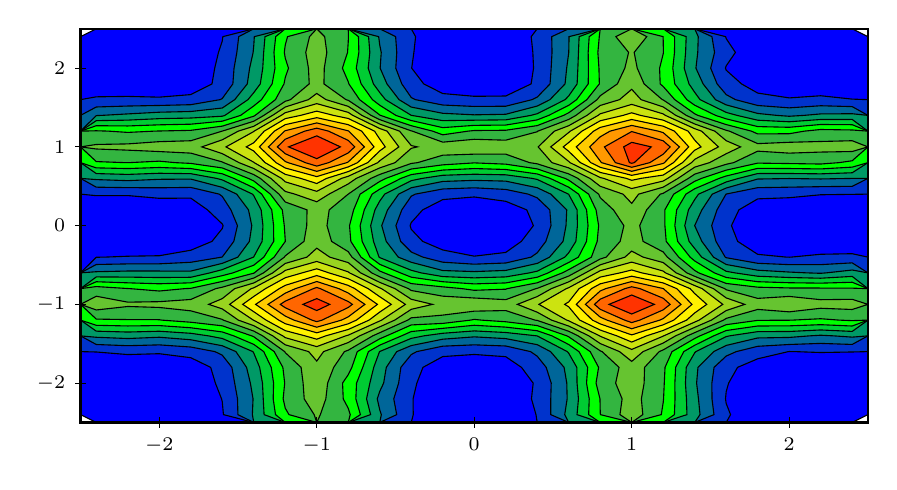
\begin{tikzpicture}
\begin{scope}[]
\pgfpathmoveto{ \pgfpointxy {0.0} {0.0}}
\pgfpathlineto{ \pgfpointxy {10.0} {0.0}}
\pgfpathlineto{ \pgfpointxy {10.0} {5.0}}
\pgfpathlineto{ \pgfpointxy {0.0} {5.0}}
\pgfpathclose
\pgfusepath{  clip, }
\begin{scope}[shift={(0.0,0.0)}]
\pgfsetxvec{\pgfpoint{2.0cm}{0cm}}
\pgfsetyvec{\pgfpoint{0cm}{1.0cm}}
\begin{scope}[shift={(2.5,2.5)}]
\begin{scope}[draw=black,fill=green!0!blue]
\pgfpathmoveto{ \pgfpointxy {-2.5} {-2.4}}
\pgfpathlineto{ \pgfpointxy {-2.5} {-2.4}}
\pgfpathlineto{ \pgfpointxy {-2.5} {-2.2}}
\pgfpathlineto{ \pgfpointxy {-2.5} {-2.0}}
\pgfpathlineto{ \pgfpointxy {-2.5} {-1.8}}
\pgfpathlineto{ \pgfpointxy {-2.5} {-1.5999999}}
\pgfpathlineto{ \pgfpointxy {-2.5} {-1.4}}
\pgfpathlineto{ \pgfpointxy {-2.5} {-1.1999999}}
\pgfpathlineto{ \pgfpointxy {-2.5} {-1.0}}
\pgfpathlineto{ \pgfpointxy {-2.5} {-0.79999995}}
\pgfpathlineto{ \pgfpointxy {-2.5} {-0.6}}
\pgfpathlineto{ \pgfpointxy {-2.5} {-0.39999986}}
\pgfpathlineto{ \pgfpointxy {-2.5} {-0.20000005}}
\pgfpathlineto{ \pgfpointxy {-2.5} {0.0}}
\pgfpathlineto{ \pgfpointxy {-2.5} {0.20000005}}
\pgfpathlineto{ \pgfpointxy {-2.5} {0.4000001}}
\pgfpathlineto{ \pgfpointxy {-2.5} {0.60000014}}
\pgfpathlineto{ \pgfpointxy {-2.5} {0.79999995}}
\pgfpathlineto{ \pgfpointxy {-2.5} {1.0}}
\pgfpathlineto{ \pgfpointxy {-2.5} {1.2}}
\pgfpathlineto{ \pgfpointxy {-2.5} {1.4000001}}
\pgfpathlineto{ \pgfpointxy {-2.5} {1.5999999}}
\pgfpathlineto{ \pgfpointxy {-2.5} {1.8000002}}
\pgfpathlineto{ \pgfpointxy {-2.5} {2.0}}
\pgfpathlineto{ \pgfpointxy {-2.5} {2.2000003}}
\pgfpathlineto{ \pgfpointxy {-2.5} {2.4}}
\pgfpathlineto{ \pgfpointxy {-2.4} {2.5}}
\pgfpathlineto{ \pgfpointxy {-2.2} {2.5}}
\pgfpathlineto{ \pgfpointxy {-2.0} {2.5}}
\pgfpathlineto{ \pgfpointxy {-1.8} {2.5}}
\pgfpathlineto{ \pgfpointxy {-1.5999999} {2.5}}
\pgfpathlineto{ \pgfpointxy {-1.4} {2.5}}
\pgfpathlineto{ \pgfpointxy {-1.1999999} {2.5}}
\pgfpathlineto{ \pgfpointxy {-1.0} {2.5}}
\pgfpathlineto{ \pgfpointxy {-0.79999995} {2.5}}
\pgfpathlineto{ \pgfpointxy {-0.6} {2.5}}
\pgfpathlineto{ \pgfpointxy {-0.39999986} {2.5}}
\pgfpathlineto{ \pgfpointxy {-0.20000005} {2.5}}
\pgfpathlineto{ \pgfpointxy {0.0} {2.5}}
\pgfpathlineto{ \pgfpointxy {0.20000005} {2.5}}
\pgfpathlineto{ \pgfpointxy {0.4000001} {2.5}}
\pgfpathlineto{ \pgfpointxy {0.60000014} {2.5}}
\pgfpathlineto{ \pgfpointxy {0.79999995} {2.5}}
\pgfpathlineto{ \pgfpointxy {1.0} {2.5}}
\pgfpathlineto{ \pgfpointxy {1.2} {2.5}}
\pgfpathlineto{ \pgfpointxy {1.4000001} {2.5}}
\pgfpathlineto{ \pgfpointxy {1.5999999} {2.5}}
\pgfpathlineto{ \pgfpointxy {1.8000002} {2.5}}
\pgfpathlineto{ \pgfpointxy {2.0} {2.5}}
\pgfpathlineto{ \pgfpointxy {2.2000003} {2.5}}
\pgfpathlineto{ \pgfpointxy {2.4} {2.5}}
\pgfpathlineto{ \pgfpointxy {2.5} {2.4}}
\pgfpathlineto{ \pgfpointxy {2.5} {2.2000003}}
\pgfpathlineto{ \pgfpointxy {2.5} {2.0}}
\pgfpathlineto{ \pgfpointxy {2.5} {1.8000002}}
\pgfpathlineto{ \pgfpointxy {2.5} {1.5999999}}
\pgfpathlineto{ \pgfpointxy {2.5} {1.4000001}}
\pgfpathlineto{ \pgfpointxy {2.5} {1.2}}
\pgfpathlineto{ \pgfpointxy {2.5} {1.0}}
\pgfpathlineto{ \pgfpointxy {2.5} {0.79999995}}
\pgfpathlineto{ \pgfpointxy {2.5} {0.60000014}}
\pgfpathlineto{ \pgfpointxy {2.5} {0.4000001}}
\pgfpathlineto{ \pgfpointxy {2.5} {0.20000005}}
\pgfpathlineto{ \pgfpointxy {2.5} {0.0}}
\pgfpathlineto{ \pgfpointxy {2.5} {-0.20000005}}
\pgfpathlineto{ \pgfpointxy {2.5} {-0.39999986}}
\pgfpathlineto{ \pgfpointxy {2.5} {-0.6}}
\pgfpathlineto{ \pgfpointxy {2.5} {-0.79999995}}
\pgfpathlineto{ \pgfpointxy {2.5} {-1.0}}
\pgfpathlineto{ \pgfpointxy {2.5} {-1.1999999}}
\pgfpathlineto{ \pgfpointxy {2.5} {-1.4}}
\pgfpathlineto{ \pgfpointxy {2.5} {-1.5999999}}
\pgfpathlineto{ \pgfpointxy {2.5} {-1.8}}
\pgfpathlineto{ \pgfpointxy {2.5} {-2.0}}
\pgfpathlineto{ \pgfpointxy {2.5} {-2.2}}
\pgfpathlineto{ \pgfpointxy {2.5} {-2.4}}
\pgfpathlineto{ \pgfpointxy {2.4} {-2.5}}
\pgfpathlineto{ \pgfpointxy {2.2000003} {-2.5}}
\pgfpathlineto{ \pgfpointxy {2.0} {-2.5}}
\pgfpathlineto{ \pgfpointxy {1.8000002} {-2.5}}
\pgfpathlineto{ \pgfpointxy {1.5999999} {-2.5}}
\pgfpathlineto{ \pgfpointxy {1.4000001} {-2.5}}
\pgfpathlineto{ \pgfpointxy {1.2} {-2.5}}
\pgfpathlineto{ \pgfpointxy {1.0} {-2.5}}
\pgfpathlineto{ \pgfpointxy {0.79999995} {-2.5}}
\pgfpathlineto{ \pgfpointxy {0.60000014} {-2.5}}
\pgfpathlineto{ \pgfpointxy {0.4000001} {-2.5}}
\pgfpathlineto{ \pgfpointxy {0.20000005} {-2.5}}
\pgfpathlineto{ \pgfpointxy {0.0} {-2.5}}
\pgfpathlineto{ \pgfpointxy {-0.20000005} {-2.5}}
\pgfpathlineto{ \pgfpointxy {-0.39999986} {-2.5}}
\pgfpathlineto{ \pgfpointxy {-0.6} {-2.5}}
\pgfpathlineto{ \pgfpointxy {-0.79999995} {-2.5}}
\pgfpathlineto{ \pgfpointxy {-1.0} {-2.5}}
\pgfpathlineto{ \pgfpointxy {-1.1999999} {-2.5}}
\pgfpathlineto{ \pgfpointxy {-1.4} {-2.5}}
\pgfpathlineto{ \pgfpointxy {-1.5999999} {-2.5}}
\pgfpathlineto{ \pgfpointxy {-1.8} {-2.5}}
\pgfpathlineto{ \pgfpointxy {-2.0} {-2.5}}
\pgfpathlineto{ \pgfpointxy {-2.2} {-2.5}}
\pgfpathlineto{ \pgfpointxy {-2.4} {-2.5}}
\pgfpathclose
\pgfusepath{ stroke, fill, }
\end{scope}
\begin{scope}[draw=black,fill=green!20!blue]
\pgfpathmoveto{ \pgfpointxy {-2.5} {-1.5999999}}
\pgfpathlineto{ \pgfpointxy {-2.5} {-1.5999999}}
\pgfpathlineto{ \pgfpointxy {-2.5} {-1.4}}
\pgfpathlineto{ \pgfpointxy {-2.5} {-1.1999999}}
\pgfpathlineto{ \pgfpointxy {-2.5} {-1.0}}
\pgfpathlineto{ \pgfpointxy {-2.5} {-0.79999995}}
\pgfpathlineto{ \pgfpointxy {-2.5} {-0.6}}
\pgfpathlineto{ \pgfpointxy {-2.4} {-0.40160170033316067}}
\pgfpathlineto{ \pgfpointxy {-2.3451851828782644} {-0.39999986}}
\pgfpathlineto{ \pgfpointxy {-2.2} {-0.38853798023267094}}
\pgfpathlineto{ \pgfpointxy {-2.0} {-0.3822968872112722}}
\pgfpathlineto{ \pgfpointxy {-1.8} {-0.31263678332614653}}
\pgfpathlineto{ \pgfpointxy {-1.6652380827991735} {-0.20000005}}
\pgfpathlineto{ \pgfpointxy {-1.5999999} {-0.03762959293745194}}
\pgfpathlineto{ \pgfpointxy {-1.594555184792923} {0.0}}
\pgfpathlineto{ \pgfpointxy {-1.5999999} {0.021166704234977463}}
\pgfpathlineto{ \pgfpointxy {-1.6935076132546583} {0.20000005}}
\pgfpathlineto{ \pgfpointxy {-1.8} {0.34948016478472166}}
\pgfpathlineto{ \pgfpointxy {-2.0} {0.3469652165524404}}
\pgfpathlineto{ \pgfpointxy {-2.2} {0.3818391234025187}}
\pgfpathlineto{ \pgfpointxy {-2.4} {0.38045202032320935}}
\pgfpathlineto{ \pgfpointxy {-2.5} {0.4000001}}
\pgfpathlineto{ \pgfpointxy {-2.5} {0.60000014}}
\pgfpathlineto{ \pgfpointxy {-2.5} {0.79999995}}
\pgfpathlineto{ \pgfpointxy {-2.5} {1.0}}
\pgfpathlineto{ \pgfpointxy {-2.5} {1.2}}
\pgfpathlineto{ \pgfpointxy {-2.5} {1.4000001}}
\pgfpathlineto{ \pgfpointxy {-2.5} {1.5999999}}
\pgfpathlineto{ \pgfpointxy {-2.4} {1.635767257394929}}
\pgfpathlineto{ \pgfpointxy {-2.2} {1.641137012612142}}
\pgfpathlineto{ \pgfpointxy {-2.0} {1.6315054379083138}}
\pgfpathlineto{ \pgfpointxy {-1.8} {1.6640936293012913}}
\pgfpathlineto{ \pgfpointxy {-1.6652753498804742} {1.8000002}}
\pgfpathlineto{ \pgfpointxy {-1.6479629502666218} {2.0}}
\pgfpathlineto{ \pgfpointxy {-1.6240220255144044} {2.2000003}}
\pgfpathlineto{ \pgfpointxy {-1.5999999} {2.3453334055344266}}
\pgfpathlineto{ \pgfpointxy {-1.5961091205760536} {2.4}}
\pgfpathlineto{ \pgfpointxy {-1.4} {2.5}}
\pgfpathlineto{ \pgfpointxy {-1.1999999} {2.5}}
\pgfpathlineto{ \pgfpointxy {-1.0} {2.5}}
\pgfpathlineto{ \pgfpointxy {-0.79999995} {2.5}}
\pgfpathlineto{ \pgfpointxy {-0.6} {2.5}}
\pgfpathlineto{ \pgfpointxy {-0.39999986} {2.5}}
\pgfpathlineto{ \pgfpointxy {-0.37238841973968695} {2.4}}
\pgfpathlineto{ \pgfpointxy {-0.3832748222595068} {2.2000003}}
\pgfpathlineto{ \pgfpointxy {-0.3971604624924101} {2.0}}
\pgfpathlineto{ \pgfpointxy {-0.32071791624411583} {1.8000002}}
\pgfpathlineto{ \pgfpointxy {-0.20000005} {1.6773958955813821}}
\pgfpathlineto{ \pgfpointxy {0.0} {1.6424533950606985}}
\pgfpathlineto{ \pgfpointxy {0.20000005} {1.6460060677863098}}
\pgfpathlineto{ \pgfpointxy {0.3612579042712847} {1.8000002}}
\pgfpathlineto{ \pgfpointxy {0.37655918264901755} {2.0}}
\pgfpathlineto{ \pgfpointxy {0.372212927953369} {2.2000003}}
\pgfpathlineto{ \pgfpointxy {0.36166670930882283} {2.4}}
\pgfpathlineto{ \pgfpointxy {0.4000001} {2.5}}
\pgfpathlineto{ \pgfpointxy {0.60000014} {2.5}}
\pgfpathlineto{ \pgfpointxy {0.79999995} {2.5}}
\pgfpathlineto{ \pgfpointxy {1.0} {2.5}}
\pgfpathlineto{ \pgfpointxy {1.2} {2.5}}
\pgfpathlineto{ \pgfpointxy {1.4000001} {2.5}}
\pgfpathlineto{ \pgfpointxy {1.5960327808720445} {2.4}}
\pgfpathlineto{ \pgfpointxy {1.5999999} {2.3741334059635797}}
\pgfpathlineto{ \pgfpointxy {1.658434066439769} {2.2000003}}
\pgfpathlineto{ \pgfpointxy {1.5999999} {2.029281113243181}}
\pgfpathlineto{ \pgfpointxy {1.5950552486590466} {2.0}}
\pgfpathlineto{ \pgfpointxy {1.5999999} {1.9738012362554755}}
\pgfpathlineto{ \pgfpointxy {1.6971242455485598} {1.8000002}}
\pgfpathlineto{ \pgfpointxy {1.8000002} {1.6834074697450356}}
\pgfpathlineto{ \pgfpointxy {2.0} {1.621968315390367}}
\pgfpathlineto{ \pgfpointxy {2.2000003} {1.649351913682013}}
\pgfpathlineto{ \pgfpointxy {2.4} {1.6067302199252067}}
\pgfpathlineto{ \pgfpointxy {2.5} {1.5999999}}
\pgfpathlineto{ \pgfpointxy {2.5} {1.4000001}}
\pgfpathlineto{ \pgfpointxy {2.5} {1.2}}
\pgfpathlineto{ \pgfpointxy {2.5} {1.0}}
\pgfpathlineto{ \pgfpointxy {2.5} {0.79999995}}
\pgfpathlineto{ \pgfpointxy {2.5} {0.60000014}}
\pgfpathlineto{ \pgfpointxy {2.5} {0.4000001}}
\pgfpathlineto{ \pgfpointxy {2.4} {0.39726194793447167}}
\pgfpathlineto{ \pgfpointxy {2.2000003} {0.3920468267205863}}
\pgfpathlineto{ \pgfpointxy {2.0} {0.3544904006619425}}
\pgfpathlineto{ \pgfpointxy {1.8000002} {0.3397740536153653}}
\pgfpathlineto{ \pgfpointxy {1.6804831540814922} {0.20000005}}
\pgfpathlineto{ \pgfpointxy {1.633387595467613} {0.0}}
\pgfpathlineto{ \pgfpointxy {1.6727044646938642} {-0.20000005}}
\pgfpathlineto{ \pgfpointxy {1.8000002} {-0.3645528137078129}}
\pgfpathlineto{ \pgfpointxy {1.9816667334487041} {-0.39999986}}
\pgfpathlineto{ \pgfpointxy {2.0} {-0.40097774649990914}}
\pgfpathlineto{ \pgfpointxy {2.011733400563399} {-0.39999986}}
\pgfpathlineto{ \pgfpointxy {2.2000003} {-0.3637948399629347}}
\pgfpathlineto{ \pgfpointxy {2.4} {-0.35664038800896014}}
\pgfpathlineto{ \pgfpointxy {2.5} {-0.39999986}}
\pgfpathlineto{ \pgfpointxy {2.5} {-0.6}}
\pgfpathlineto{ \pgfpointxy {2.5} {-0.79999995}}
\pgfpathlineto{ \pgfpointxy {2.5} {-1.0}}
\pgfpathlineto{ \pgfpointxy {2.5} {-1.1999999}}
\pgfpathlineto{ \pgfpointxy {2.5} {-1.4}}
\pgfpathlineto{ \pgfpointxy {2.5} {-1.5999999}}
\pgfpathlineto{ \pgfpointxy {2.4} {-1.6046913446835531}}
\pgfpathlineto{ \pgfpointxy {2.2000003} {-1.6115634085901718}}
\pgfpathlineto{ \pgfpointxy {2.036666734268268} {-1.5999999}}
\pgfpathlineto{ \pgfpointxy {2.0} {-1.5990717165329285}}
\pgfpathlineto{ \pgfpointxy {1.994465475777785} {-1.5999999}}
\pgfpathlineto{ \pgfpointxy {1.8000002} {-1.6912094274761051}}
\pgfpathlineto{ \pgfpointxy {1.6719445066112604} {-1.8}}
\pgfpathlineto{ \pgfpointxy {1.6153754366992477} {-2.0}}
\pgfpathlineto{ \pgfpointxy {1.5999999} {-2.1066666608055433}}
\pgfpathlineto{ \pgfpointxy {1.5954748085020771} {-2.2}}
\pgfpathlineto{ \pgfpointxy {1.5999999} {-2.259733329753081}}
\pgfpathlineto{ \pgfpointxy {1.6276116100626359} {-2.4}}
\pgfpathlineto{ \pgfpointxy {1.5999999} {-2.5}}
\pgfpathlineto{ \pgfpointxy {1.4000001} {-2.5}}
\pgfpathlineto{ \pgfpointxy {1.2} {-2.5}}
\pgfpathlineto{ \pgfpointxy {1.0} {-2.5}}
\pgfpathlineto{ \pgfpointxy {0.79999995} {-2.5}}
\pgfpathlineto{ \pgfpointxy {0.60000014} {-2.5}}
\pgfpathlineto{ \pgfpointxy {0.4000001} {-2.5}}
\pgfpathlineto{ \pgfpointxy {0.3919764442737472} {-2.4}}
\pgfpathlineto{ \pgfpointxy {0.36338312724484734} {-2.2}}
\pgfpathlineto{ \pgfpointxy {0.3742773289657624} {-2.0}}
\pgfpathlineto{ \pgfpointxy {0.29995276039867} {-1.8}}
\pgfpathlineto{ \pgfpointxy {0.20000005} {-1.6644871670370684}}
\pgfpathlineto{ \pgfpointxy {0.0} {-1.6361904633187114}}
\pgfpathlineto{ \pgfpointxy {-0.20000005} {-1.6630666541953882}}
\pgfpathlineto{ \pgfpointxy {-0.3256268789143011} {-1.8}}
\pgfpathlineto{ \pgfpointxy {-0.36451440387432354} {-2.0}}
\pgfpathlineto{ \pgfpointxy {-0.38853798023267094} {-2.2}}
\pgfpathlineto{ \pgfpointxy {-0.38733890409312677} {-2.4}}
\pgfpathlineto{ \pgfpointxy {-0.39999986} {-2.5}}
\pgfpathlineto{ \pgfpointxy {-0.6} {-2.5}}
\pgfpathlineto{ \pgfpointxy {-0.79999995} {-2.5}}
\pgfpathlineto{ \pgfpointxy {-1.0} {-2.5}}
\pgfpathlineto{ \pgfpointxy {-1.1999999} {-2.5}}
\pgfpathlineto{ \pgfpointxy {-1.4} {-2.5}}
\pgfpathlineto{ \pgfpointxy {-1.5925540990321152} {-2.4}}
\pgfpathlineto{ \pgfpointxy {-1.5999999} {-2.236190472259408}}
\pgfpathlineto{ \pgfpointxy {-1.6044837624669779} {-2.2}}
\pgfpathlineto{ \pgfpointxy {-1.6437530736606796} {-2.0}}
\pgfpathlineto{ \pgfpointxy {-1.6735353412200706} {-1.8}}
\pgfpathlineto{ \pgfpointxy {-1.8} {-1.6772548897009272}}
\pgfpathlineto{ \pgfpointxy {-2.0} {-1.6264533203164735}}
\pgfpathlineto{ \pgfpointxy {-2.2} {-1.6374554578849985}}
\pgfpathlineto{ \pgfpointxy {-2.4} {-1.6047798608740171}}
\pgfpathclose
\pgfpathmoveto{ \pgfpointxy {-0.327429993071477} {0.20000005}}
\pgfpathlineto{ \pgfpointxy {-0.327429993071477} {0.20000005}}
\pgfpathlineto{ \pgfpointxy {-0.39999986} {0.03887009432928723}}
\pgfpathlineto{ \pgfpointxy {-0.4073035781582197} {0.0}}
\pgfpathlineto{ \pgfpointxy {-0.39999986} {-0.046802684532947225}}
\pgfpathlineto{ \pgfpointxy {-0.32782048045251644} {-0.20000005}}
\pgfpathlineto{ \pgfpointxy {-0.20000005} {-0.30896171598486566}}
\pgfpathlineto{ \pgfpointxy {0.0} {-0.38790120309517695}}
\pgfpathlineto{ \pgfpointxy {0.20000005} {-0.34033666815520913}}
\pgfpathlineto{ \pgfpointxy {0.29923813694999346} {-0.20000005}}
\pgfpathlineto{ \pgfpointxy {0.37571934109717064} {0.0}}
\pgfpathlineto{ \pgfpointxy {0.3335757997993265} {0.20000005}}
\pgfpathlineto{ \pgfpointxy {0.20000005} {0.30883954802780966}}
\pgfpathlineto{ \pgfpointxy {0.0} {0.3641111537896924}}
\pgfpathlineto{ \pgfpointxy {-0.20000005} {0.33041670884316154}}
\pgfpathclose
\pgfusepath{ stroke, fill, }
\end{scope}
\begin{scope}[draw=black,fill=green!40!blue]
\pgfpathmoveto{ \pgfpointxy {-2.5} {-1.4}}
\pgfpathlineto{ \pgfpointxy {-2.5} {-1.4}}
\pgfpathlineto{ \pgfpointxy {-2.5} {-1.1999999}}
\pgfpathlineto{ \pgfpointxy {-2.5} {-1.0}}
\pgfpathlineto{ \pgfpointxy {-2.5} {-0.79999995}}
\pgfpathlineto{ \pgfpointxy {-2.5} {-0.6}}
\pgfpathlineto{ \pgfpointxy {-2.4} {-0.49346317356347535}}
\pgfpathlineto{ \pgfpointxy {-2.2} {-0.4862193523139493}}
\pgfpathlineto{ \pgfpointxy {-2.0} {-0.48502161499612795}}
\pgfpathlineto{ \pgfpointxy {-1.8} {-0.46555991698355825}}
\pgfpathlineto{ \pgfpointxy {-1.6025396691664817} {-0.39999986}}
\pgfpathlineto{ \pgfpointxy {-1.5999999} {-0.3979873900612194}}
\pgfpathlineto{ \pgfpointxy {-1.526620032115555} {-0.20000005}}
\pgfpathlineto{ \pgfpointxy {-1.5035798350985923} {0.0}}
\pgfpathlineto{ \pgfpointxy {-1.5449343689705128} {0.20000005}}
\pgfpathlineto{ \pgfpointxy {-1.5999999} {0.37056914846586997}}
\pgfpathlineto{ \pgfpointxy {-1.6191534260278027} {0.4000001}}
\pgfpathlineto{ \pgfpointxy {-1.8} {0.48534336533402067}}
\pgfpathlineto{ \pgfpointxy {-2.0} {0.48055771234786393}}
\pgfpathlineto{ \pgfpointxy {-2.2} {0.48234805282619275}}
\pgfpathlineto{ \pgfpointxy {-2.4} {0.48839006720621825}}
\pgfpathlineto{ \pgfpointxy {-2.5} {0.60000014}}
\pgfpathlineto{ \pgfpointxy {-2.5} {0.79999995}}
\pgfpathlineto{ \pgfpointxy {-2.5} {1.0}}
\pgfpathlineto{ \pgfpointxy {-2.5} {1.2}}
\pgfpathlineto{ \pgfpointxy {-2.5} {1.4000001}}
\pgfpathlineto{ \pgfpointxy {-2.4} {1.5067190139531315}}
\pgfpathlineto{ \pgfpointxy {-2.2} {1.5187750893308216}}
\pgfpathlineto{ \pgfpointxy {-2.0} {1.5261010700945903}}
\pgfpathlineto{ \pgfpointxy {-1.8} {1.535820651371849}}
\pgfpathlineto{ \pgfpointxy {-1.6142772729373962} {1.5999999}}
\pgfpathlineto{ \pgfpointxy {-1.5999999} {1.6144048232141701}}
\pgfpathlineto{ \pgfpointxy {-1.5327292196749998} {1.8000002}}
\pgfpathlineto{ \pgfpointxy {-1.525221430696113} {2.0}}
\pgfpathlineto{ \pgfpointxy {-1.507347917081811} {2.2000003}}
\pgfpathlineto{ \pgfpointxy {-1.4954211000958513} {2.4}}
\pgfpathlineto{ \pgfpointxy {-1.4} {2.5}}
\pgfpathlineto{ \pgfpointxy {-1.1999999} {2.5}}
\pgfpathlineto{ \pgfpointxy {-1.0} {2.5}}
\pgfpathlineto{ \pgfpointxy {-0.79999995} {2.5}}
\pgfpathlineto{ \pgfpointxy {-0.6} {2.5}}
\pgfpathlineto{ \pgfpointxy {-0.49914663685162886} {2.4}}
\pgfpathlineto{ \pgfpointxy {-0.4919395751879052} {2.2000003}}
\pgfpathlineto{ \pgfpointxy {-0.49819880058019494} {2.0}}
\pgfpathlineto{ \pgfpointxy {-0.4599555251565244} {1.8000002}}
\pgfpathlineto{ \pgfpointxy {-0.39999986} {1.6270513435491383}}
\pgfpathlineto{ \pgfpointxy {-0.3734590878089272} {1.5999999}}
\pgfpathlineto{ \pgfpointxy {-0.20000005} {1.5316481393823098}}
\pgfpathlineto{ \pgfpointxy {0.0} {1.5135840197068111}}
\pgfpathlineto{ \pgfpointxy {0.20000005} {1.5162936819894366}}
\pgfpathlineto{ \pgfpointxy {0.36681059427755924} {1.5999999}}
\pgfpathlineto{ \pgfpointxy {0.4000001} {1.632037098609187}}
\pgfpathlineto{ \pgfpointxy {0.48143663253012203} {1.8000002}}
\pgfpathlineto{ \pgfpointxy {0.48845532908429945} {2.0}}
\pgfpathlineto{ \pgfpointxy {0.49393488170583755} {2.2000003}}
\pgfpathlineto{ \pgfpointxy {0.492073535399018} {2.4}}
\pgfpathlineto{ \pgfpointxy {0.60000014} {2.5}}
\pgfpathlineto{ \pgfpointxy {0.79999995} {2.5}}
\pgfpathlineto{ \pgfpointxy {1.0} {2.5}}
\pgfpathlineto{ \pgfpointxy {1.2} {2.5}}
\pgfpathlineto{ \pgfpointxy {1.4000001} {2.5}}
\pgfpathlineto{ \pgfpointxy {1.5092434135256125} {2.4}}
\pgfpathlineto{ \pgfpointxy {1.5260881103078523} {2.2000003}}
\pgfpathlineto{ \pgfpointxy {1.5013687130466726} {2.0}}
\pgfpathlineto{ \pgfpointxy {1.5421803537342287} {1.8000002}}
\pgfpathlineto{ \pgfpointxy {1.5999999} {1.663802531181294}}
\pgfpathlineto{ \pgfpointxy {1.6585941662762709} {1.5999999}}
\pgfpathlineto{ \pgfpointxy {1.8000002} {1.5257619647504317}}
\pgfpathlineto{ \pgfpointxy {2.0} {1.4956359363803107}}
\pgfpathlineto{ \pgfpointxy {2.2000003} {1.522393222331492}}
\pgfpathlineto{ \pgfpointxy {2.4} {1.5115812563584141}}
\pgfpathlineto{ \pgfpointxy {2.5} {1.4000001}}
\pgfpathlineto{ \pgfpointxy {2.5} {1.2}}
\pgfpathlineto{ \pgfpointxy {2.5} {1.0}}
\pgfpathlineto{ \pgfpointxy {2.5} {0.79999995}}
\pgfpathlineto{ \pgfpointxy {2.5} {0.60000014}}
\pgfpathlineto{ \pgfpointxy {2.4} {0.49924354351017763}}
\pgfpathlineto{ \pgfpointxy {2.2000003} {0.49476359710526996}}
\pgfpathlineto{ \pgfpointxy {2.0} {0.48832045796613643}}
\pgfpathlineto{ \pgfpointxy {1.8000002} {0.4821189074861292}}
\pgfpathlineto{ \pgfpointxy {1.5999999} {0.40104792037441994}}
\pgfpathlineto{ \pgfpointxy {1.5988066454391179} {0.4000001}}
\pgfpathlineto{ \pgfpointxy {1.5415420103370465} {0.20000005}}
\pgfpathlineto{ \pgfpointxy {1.5076845380906532} {0.0}}
\pgfpathlineto{ \pgfpointxy {1.53485238079909} {-0.20000005}}
\pgfpathlineto{ \pgfpointxy {1.5937027874740997} {-0.39999986}}
\pgfpathlineto{ \pgfpointxy {1.5999999} {-0.4072763915802162}}
\pgfpathlineto{ \pgfpointxy {1.8000002} {-0.47859646110681053}}
\pgfpathlineto{ \pgfpointxy {2.0} {-0.49528885901636555}}
\pgfpathlineto{ \pgfpointxy {2.2000003} {-0.4954925477283525}}
\pgfpathlineto{ \pgfpointxy {2.4} {-0.4730341578300439}}
\pgfpathlineto{ \pgfpointxy {2.5} {-0.6}}
\pgfpathlineto{ \pgfpointxy {2.5} {-0.79999995}}
\pgfpathlineto{ \pgfpointxy {2.5} {-1.0}}
\pgfpathlineto{ \pgfpointxy {2.5} {-1.1999999}}
\pgfpathlineto{ \pgfpointxy {2.5} {-1.4}}
\pgfpathlineto{ \pgfpointxy {2.4} {-1.50889616009479}}
\pgfpathlineto{ \pgfpointxy {2.2000003} {-1.4958043608406948}}
\pgfpathlineto{ \pgfpointxy {2.0} {-1.5095358502198373}}
\pgfpathlineto{ \pgfpointxy {1.8000002} {-1.5326341928260754}}
\pgfpathlineto{ \pgfpointxy {1.6637374357818953} {-1.5999999}}
\pgfpathlineto{ \pgfpointxy {1.5999999} {-1.6564653118151413}}
\pgfpathlineto{ \pgfpointxy {1.5227918770321152} {-1.8}}
\pgfpathlineto{ \pgfpointxy {1.508949831427504} {-2.0}}
\pgfpathlineto{ \pgfpointxy {1.5097374334871168} {-2.2}}
\pgfpathlineto{ \pgfpointxy {1.522298910511636} {-2.4}}
\pgfpathlineto{ \pgfpointxy {1.4000001} {-2.5}}
\pgfpathlineto{ \pgfpointxy {1.2} {-2.5}}
\pgfpathlineto{ \pgfpointxy {1.0} {-2.5}}
\pgfpathlineto{ \pgfpointxy {0.79999995} {-2.5}}
\pgfpathlineto{ \pgfpointxy {0.60000014} {-2.5}}
\pgfpathlineto{ \pgfpointxy {0.4858516641373791} {-2.4}}
\pgfpathlineto{ \pgfpointxy {0.48598043665143775} {-2.2}}
\pgfpathlineto{ \pgfpointxy {0.48876461330063137} {-2.0}}
\pgfpathlineto{ \pgfpointxy {0.45697460898872677} {-1.8}}
\pgfpathlineto{ \pgfpointxy {0.4000001} {-1.6581333207885425}}
\pgfpathlineto{ \pgfpointxy {0.3575669525567342} {-1.5999999}}
\pgfpathlineto{ \pgfpointxy {0.20000005} {-1.5285209568262628}}
\pgfpathlineto{ \pgfpointxy {0.0} {-1.5140262696567117}}
\pgfpathlineto{ \pgfpointxy {-0.20000005} {-1.5310762656037087}}
\pgfpathlineto{ \pgfpointxy {-0.36531325139870896} {-1.5999999}}
\pgfpathlineto{ \pgfpointxy {-0.39999986} {-1.6372042882186109}}
\pgfpathlineto{ \pgfpointxy {-0.465969468601259} {-1.8}}
\pgfpathlineto{ \pgfpointxy {-0.4800897566574456} {-2.0}}
\pgfpathlineto{ \pgfpointxy {-0.51105621178904} {-2.2}}
\pgfpathlineto{ \pgfpointxy {-0.49236778617590327} {-2.4}}
\pgfpathlineto{ \pgfpointxy {-0.6} {-2.5}}
\pgfpathlineto{ \pgfpointxy {-0.79999995} {-2.5}}
\pgfpathlineto{ \pgfpointxy {-1.0} {-2.5}}
\pgfpathlineto{ \pgfpointxy {-1.1999999} {-2.5}}
\pgfpathlineto{ \pgfpointxy {-1.4} {-2.5}}
\pgfpathlineto{ \pgfpointxy {-1.5006926258018005} {-2.4}}
\pgfpathlineto{ \pgfpointxy {-1.5031823312554349} {-2.2}}
\pgfpathlineto{ \pgfpointxy {-1.5211736943345393} {-2.0}}
\pgfpathlineto{ \pgfpointxy {-1.5388596348006995} {-1.8}}
\pgfpathlineto{ \pgfpointxy {-1.5999999} {-1.6451110983722739}}
\pgfpathlineto{ \pgfpointxy {-1.646666653951009} {-1.5999999}}
\pgfpathlineto{ \pgfpointxy {-1.8} {-1.5418736240670312}}
\pgfpathlineto{ \pgfpointxy {-2.0} {-1.5144292090581433}}
\pgfpathlineto{ \pgfpointxy {-2.2} {-1.524801700366591}}
\pgfpathlineto{ \pgfpointxy {-2.4} {-1.5097835350281748}}
\pgfpathclose
\pgfpathmoveto{ \pgfpointxy {-0.37465462298454133} {0.4000001}}
\pgfpathlineto{ \pgfpointxy {-0.37465462298454133} {0.4000001}}
\pgfpathlineto{ \pgfpointxy {-0.39999986} {0.373950660109152}}
\pgfpathlineto{ \pgfpointxy {-0.46002126885647465} {0.20000005}}
\pgfpathlineto{ \pgfpointxy {-0.4974097366134327} {0.0}}
\pgfpathlineto{ \pgfpointxy {-0.46727073562151666} {-0.20000005}}
\pgfpathlineto{ \pgfpointxy {-0.39999986} {-0.33497832271701844}}
\pgfpathlineto{ \pgfpointxy {-0.32637251663003486} {-0.39999986}}
\pgfpathlineto{ \pgfpointxy {-0.20000005} {-0.46436950774414587}}
\pgfpathlineto{ \pgfpointxy {0.0} {-0.48965666993280843}}
\pgfpathlineto{ \pgfpointxy {0.20000005} {-0.4746221920417413}}
\pgfpathlineto{ \pgfpointxy {0.3610551985083439} {-0.39999986}}
\pgfpathlineto{ \pgfpointxy {0.4000001} {-0.34476187264635483}}
\pgfpathlineto{ \pgfpointxy {0.4547748188043501} {-0.20000005}}
\pgfpathlineto{ \pgfpointxy {0.48749723868103834} {0.0}}
\pgfpathlineto{ \pgfpointxy {0.4797972560627679} {0.20000005}}
\pgfpathlineto{ \pgfpointxy {0.4000001} {0.3531873904476779}}
\pgfpathlineto{ \pgfpointxy {0.34273813759819394} {0.4000001}}
\pgfpathlineto{ \pgfpointxy {0.20000005} {0.45965178539578}}
\pgfpathlineto{ \pgfpointxy {0.0} {0.4802230098491398}}
\pgfpathlineto{ \pgfpointxy {-0.20000005} {0.46549553968482194}}
\pgfpathclose
\pgfusepath{ stroke, fill, }
\end{scope}
\begin{scope}[draw=black,fill=green!60!blue]
\pgfpathmoveto{ \pgfpointxy {-2.5} {-1.4}}
\pgfpathlineto{ \pgfpointxy {-2.5} {-1.4}}
\pgfpathlineto{ \pgfpointxy {-2.5} {-1.1999999}}
\pgfpathlineto{ \pgfpointxy {-2.5} {-1.0}}
\pgfpathlineto{ \pgfpointxy {-2.5} {-0.79999995}}
\pgfpathlineto{ \pgfpointxy {-2.5} {-0.6}}
\pgfpathlineto{ \pgfpointxy {-2.4} {-0.5853246467937898}}
\pgfpathlineto{ \pgfpointxy {-2.2} {-0.5766133898696579}}
\pgfpathlineto{ \pgfpointxy {-2.0} {-0.5768830882264424}}
\pgfpathlineto{ \pgfpointxy {-1.8} {-0.5773912756987238}}
\pgfpathlineto{ \pgfpointxy {-1.5999999} {-0.4790985614355181}}
\pgfpathlineto{ \pgfpointxy {-1.5011267456790092} {-0.39999986}}
\pgfpathlineto{ \pgfpointxy {-1.427692291713678} {-0.20000005}}
\pgfpathlineto{ \pgfpointxy {-1.4126044854042614} {0.0}}
\pgfpathlineto{ \pgfpointxy {-1.433543291195171} {0.20000005}}
\pgfpathlineto{ \pgfpointxy {-1.5082269355760398} {0.4000001}}
\pgfpathlineto{ \pgfpointxy {-1.5999999} {0.48626671116550746}}
\pgfpathlineto{ \pgfpointxy {-1.8} {0.5913109074873426}}
\pgfpathlineto{ \pgfpointxy {-2.0} {0.5881369281461031}}
\pgfpathlineto{ \pgfpointxy {-2.2} {0.5713208004832269}}
\pgfpathlineto{ \pgfpointxy {-2.4} {0.5846258963046429}}
\pgfpathlineto{ \pgfpointxy {-2.5} {0.60000014}}
\pgfpathlineto{ \pgfpointxy {-2.5} {0.79999995}}
\pgfpathlineto{ \pgfpointxy {-2.5} {1.0}}
\pgfpathlineto{ \pgfpointxy {-2.5} {1.2}}
\pgfpathlineto{ \pgfpointxy {-2.4} {1.3975455126234078}}
\pgfpathlineto{ \pgfpointxy {-2.36624999800697} {1.4000001}}
\pgfpathlineto{ \pgfpointxy {-2.2} {1.418798644967087}}
\pgfpathlineto{ \pgfpointxy {-2.0} {1.4403636950796304}}
\pgfpathlineto{ \pgfpointxy {-1.8} {1.4492966949347328}}
\pgfpathlineto{ \pgfpointxy {-1.5999999} {1.493705238793713}}
\pgfpathlineto{ \pgfpointxy {-1.5208308459433675} {1.5999999}}
\pgfpathlineto{ \pgfpointxy {-1.4411650327658192} {1.8000002}}
\pgfpathlineto{ \pgfpointxy {-1.4262936902942358} {2.0}}
\pgfpathlineto{ \pgfpointxy {-1.4040875749105086} {2.2000003}}
\pgfpathlineto{ \pgfpointxy {-1.4} {2.2861539174730963}}
\pgfpathlineto{ \pgfpointxy {-1.3964508228843733} {2.4}}
\pgfpathlineto{ \pgfpointxy {-1.1999999} {2.5}}
\pgfpathlineto{ \pgfpointxy {-1.0} {2.5}}
\pgfpathlineto{ \pgfpointxy {-0.79999995} {2.5}}
\pgfpathlineto{ \pgfpointxy {-0.6069682975834851} {2.4}}
\pgfpathlineto{ \pgfpointxy {-0.6} {2.29379317488136}}
\pgfpathlineto{ \pgfpointxy {-0.5905226196301938} {2.2000003}}
\pgfpathlineto{ \pgfpointxy {-0.5974736558606748} {2.0}}
\pgfpathlineto{ \pgfpointxy {-0.5542666376729806} {1.8000002}}
\pgfpathlineto{ \pgfpointxy {-0.47744677837224714} {1.5999999}}
\pgfpathlineto{ \pgfpointxy {-0.39999986} {1.5056296893181624}}
\pgfpathlineto{ \pgfpointxy {-0.20000005} {1.426468459995927}}
\pgfpathlineto{ \pgfpointxy {0.0} {1.407218103334868}}
\pgfpathlineto{ \pgfpointxy {0.20000005} {1.4141516828741412}}
\pgfpathlineto{ \pgfpointxy {0.4000001} {1.5186254894354505}}
\pgfpathlineto{ \pgfpointxy {0.48081915704565237} {1.5999999}}
\pgfpathlineto{ \pgfpointxy {0.5767003825467443} {1.8000002}}
\pgfpathlineto{ \pgfpointxy {0.587038373526588} {2.0}}
\pgfpathlineto{ \pgfpointxy {0.60000014} {2.195789543656926}}
\pgfpathlineto{ \pgfpointxy {0.6001743381351949} {2.2000003}}
\pgfpathlineto{ \pgfpointxy {0.6019909964495116} {2.4}}
\pgfpathlineto{ \pgfpointxy {0.79999995} {2.5}}
\pgfpathlineto{ \pgfpointxy {1.0} {2.5}}
\pgfpathlineto{ \pgfpointxy {1.2} {2.5}}
\pgfpathlineto{ \pgfpointxy {1.4000001} {2.5}}
\pgfpathlineto{ \pgfpointxy {1.4224540461791806} {2.4}}
\pgfpathlineto{ \pgfpointxy {1.4193208131194117} {2.2000003}}
\pgfpathlineto{ \pgfpointxy {1.4076821774342996} {2.0}}
\pgfpathlineto{ \pgfpointxy {1.4532076060771941} {1.8000002}}
\pgfpathlineto{ \pgfpointxy {1.5319031742668896} {1.5999999}}
\pgfpathlineto{ \pgfpointxy {1.5999999} {1.5335135736175483}}
\pgfpathlineto{ \pgfpointxy {1.8000002} {1.4247143441970858}}
\pgfpathlineto{ \pgfpointxy {1.9214035746559759} {1.4000001}}
\pgfpathlineto{ \pgfpointxy {2.0} {1.3889109490383968}}
\pgfpathlineto{ \pgfpointxy {2.0933334017793337} {1.4000001}}
\pgfpathlineto{ \pgfpointxy {2.2000003} {1.4187546371485724}}
\pgfpathlineto{ \pgfpointxy {2.4} {1.4208974943233605}}
\pgfpathlineto{ \pgfpointxy {2.5} {1.4000001}}
\pgfpathlineto{ \pgfpointxy {2.5} {1.2}}
\pgfpathlineto{ \pgfpointxy {2.5} {1.0}}
\pgfpathlineto{ \pgfpointxy {2.5} {0.79999995}}
\pgfpathlineto{ \pgfpointxy {2.5} {0.60000014}}
\pgfpathlineto{ \pgfpointxy {2.4} {0.5995745142723652}}
\pgfpathlineto{ \pgfpointxy {2.2000003} {0.5926644059458819}}
\pgfpathlineto{ \pgfpointxy {2.0} {0.5979845422875973}}
\pgfpathlineto{ \pgfpointxy {1.8000002} {0.5917829918075901}}
\pgfpathlineto{ \pgfpointxy {1.5999999} {0.4777236216073115}}
\pgfpathlineto{ \pgfpointxy {1.5114815412572131} {0.4000001}}
\pgfpathlineto{ \pgfpointxy {1.4453061812386219} {0.20000005}}
\pgfpathlineto{ \pgfpointxy {1.4000001} {0.0011940671214416554}}
\pgfpathlineto{ \pgfpointxy {1.3998218843924968} {0.0}}
\pgfpathlineto{ \pgfpointxy {1.4000001} {-0.001111073874764834}}
\pgfpathlineto{ \pgfpointxy {1.4453165144859987} {-0.20000005}}
\pgfpathlineto{ \pgfpointxy {1.5190501918146353} {-0.39999986}}
\pgfpathlineto{ \pgfpointxy {1.5999999} {-0.49353655546721864}}
\pgfpathlineto{ \pgfpointxy {1.8000002} {-0.5661919216484106}}
\pgfpathlineto{ \pgfpointxy {2.0} {-0.5895999715328217}}
\pgfpathlineto{ \pgfpointxy {2.1114286401442115} {-0.6}}
\pgfpathlineto{ \pgfpointxy {2.2000003} {-0.6054745854559058}}
\pgfpathlineto{ \pgfpointxy {2.235942099556543} {-0.6}}
\pgfpathlineto{ \pgfpointxy {2.4} {-0.5637179198650979}}
\pgfpathlineto{ \pgfpointxy {2.5} {-0.6}}
\pgfpathlineto{ \pgfpointxy {2.5} {-0.79999995}}
\pgfpathlineto{ \pgfpointxy {2.5} {-1.0}}
\pgfpathlineto{ \pgfpointxy {2.5} {-1.1999999}}
\pgfpathlineto{ \pgfpointxy {2.5} {-1.4}}
\pgfpathlineto{ \pgfpointxy {2.4} {-1.416131131390079}}
\pgfpathlineto{ \pgfpointxy {2.282857214127268} {-1.4}}
\pgfpathlineto{ \pgfpointxy {2.2000003} {-1.3917730331315217}}
\pgfpathlineto{ \pgfpointxy {2.128979660813906} {-1.4}}
\pgfpathlineto{ \pgfpointxy {2.0} {-1.4199999839067459}}
\pgfpathlineto{ \pgfpointxy {1.8000002} {-1.4266666506727537}}
\pgfpathlineto{ \pgfpointxy {1.5999999} {-1.521422910319251}}
\pgfpathlineto{ \pgfpointxy {1.5204800599098203} {-1.5999999}}
\pgfpathlineto{ \pgfpointxy {1.4206498779168202} {-1.8}}
\pgfpathlineto{ \pgfpointxy {1.4120548528147072} {-2.0}}
\pgfpathlineto{ \pgfpointxy {1.4240000584721568} {-2.2}}
\pgfpathlineto{ \pgfpointxy {1.4336050742892632} {-2.4}}
\pgfpathlineto{ \pgfpointxy {1.4000001} {-2.5}}
\pgfpathlineto{ \pgfpointxy {1.2} {-2.5}}
\pgfpathlineto{ \pgfpointxy {1.0} {-2.5}}
\pgfpathlineto{ \pgfpointxy {0.79999995} {-2.5}}
\pgfpathlineto{ \pgfpointxy {0.60000014} {-2.5}}
\pgfpathlineto{ \pgfpointxy {0.5745455003597519} {-2.4}}
\pgfpathlineto{ \pgfpointxy {0.590000046044588} {-2.2}}
\pgfpathlineto{ \pgfpointxy {0.5876923537025087} {-2.0}}
\pgfpathlineto{ \pgfpointxy {0.5706024553940954} {-1.8}}
\pgfpathlineto{ \pgfpointxy {0.48451132266817254} {-1.5999999}}
\pgfpathlineto{ \pgfpointxy {0.4000001} {-1.5118431225302174}}
\pgfpathlineto{ \pgfpointxy {0.20000005} {-1.434834421213889}}
\pgfpathlineto{ \pgfpointxy {0.0} {-1.4126164712519202}}
\pgfpathlineto{ \pgfpointxy {-0.20000005} {-1.442382429381336}}
\pgfpathlineto{ \pgfpointxy {-0.39999986} {-1.5233656812398952}}
\pgfpathlineto{ \pgfpointxy {-0.4921400479015672} {-1.5999999}}
\pgfpathlineto{ \pgfpointxy {-0.5584313436173927} {-1.8}}
\pgfpathlineto{ \pgfpointxy {-0.5753535066740683} {-2.0}}
\pgfpathlineto{ \pgfpointxy {-0.6} {-2.1045714226790837}}
\pgfpathlineto{ \pgfpointxy {-0.6160191565787763} {-2.2}}
\pgfpathlineto{ \pgfpointxy {-0.6} {-2.339166664270063}}
\pgfpathlineto{ \pgfpointxy {-0.5899310060205132} {-2.4}}
\pgfpathlineto{ \pgfpointxy {-0.6} {-2.5}}
\pgfpathlineto{ \pgfpointxy {-0.79999995} {-2.5}}
\pgfpathlineto{ \pgfpointxy {-1.0} {-2.5}}
\pgfpathlineto{ \pgfpointxy {-1.1999999} {-2.5}}
\pgfpathlineto{ \pgfpointxy {-1.4} {-2.5}}
\pgfpathlineto{ \pgfpointxy {-1.408831152571486} {-2.4}}
\pgfpathlineto{ \pgfpointxy {-1.404599286813146} {-2.2}}
\pgfpathlineto{ \pgfpointxy {-1.4215492797044802} {-2.0}}
\pgfpathlineto{ \pgfpointxy {-1.4457894579752495} {-1.8}}
\pgfpathlineto{ \pgfpointxy {-1.5130037875739792} {-1.5999999}}
\pgfpathlineto{ \pgfpointxy {-1.5999999} {-1.525472298181989}}
\pgfpathlineto{ \pgfpointxy {-1.8} {-1.4494117490508978}}
\pgfpathlineto{ \pgfpointxy {-2.0} {-1.4175342304453458}}
\pgfpathlineto{ \pgfpointxy {-2.2} {-1.4338263506722604}}
\pgfpathlineto{ \pgfpointxy {-2.4} {-1.4179220617978603}}
\pgfpathclose
\pgfpathmoveto{ \pgfpointxy {-0.39999986} {-0.4655196829455299}}
\pgfpathlineto{ \pgfpointxy {-0.39999986} {-0.4655196829455299}}
\pgfpathlineto{ \pgfpointxy {-0.20000005} {-0.5703370498974671}}
\pgfpathlineto{ \pgfpointxy {0.0} {-0.5836544564940604}}
\pgfpathlineto{ \pgfpointxy {0.20000005} {-0.5689333045581977}}
\pgfpathlineto{ \pgfpointxy {0.4000001} {-0.47972122425090147}}
\pgfpathlineto{ \pgfpointxy {0.4783562087645268} {-0.39999986}}
\pgfpathlineto{ \pgfpointxy {0.564015489672832} {-0.20000005}}
\pgfpathlineto{ \pgfpointxy {0.5827609886976606} {0.0}}
\pgfpathlineto{ \pgfpointxy {0.587376471861007} {0.20000005}}
\pgfpathlineto{ \pgfpointxy {0.48648225794078837} {0.4000001}}
\pgfpathlineto{ \pgfpointxy {0.4000001} {0.4813383343882278}}
\pgfpathlineto{ \pgfpointxy {0.20000005} {0.5652239262724099}}
\pgfpathlineto{ \pgfpointxy {0.0} {0.5748495441465873}}
\pgfpathlineto{ \pgfpointxy {-0.20000005} {0.5610811266947437}}
\pgfpathlineto{ \pgfpointxy {-0.39999986} {0.48114654123783085}}
\pgfpathlineto{ \pgfpointxy {-0.47987457804825606} {0.4000001}}
\pgfpathlineto{ \pgfpointxy {-0.5504153064121835} {0.20000005}}
\pgfpathlineto{ \pgfpointxy {-0.5875158950686454} {0.0}}
\pgfpathlineto{ \pgfpointxy {-0.5588349225306972} {-0.20000005}}
\pgfpathlineto{ \pgfpointxy {-0.4823423122769004} {-0.39999986}}
\pgfpathclose
\pgfusepath{ stroke, fill, }
\end{scope}
\begin{scope}[draw=black,fill=green!80!blue]
\pgfpathmoveto{ \pgfpointxy {-2.5} {-1.1999999}}
\pgfpathlineto{ \pgfpointxy {-2.5} {-1.1999999}}
\pgfpathlineto{ \pgfpointxy {-2.5} {-1.0}}
\pgfpathlineto{ \pgfpointxy {-2.5} {-0.79999995}}
\pgfpathlineto{ \pgfpointxy {-2.4} {-0.6514574039120007}}
\pgfpathlineto{ \pgfpointxy {-2.2} {-0.6537777502669226}}
\pgfpathlineto{ \pgfpointxy {-2.0} {-0.6593090295276836}}
\pgfpathlineto{ \pgfpointxy {-1.8} {-0.6560132066002062}}
\pgfpathlineto{ \pgfpointxy {-1.6786379805922935} {-0.6}}
\pgfpathlineto{ \pgfpointxy {-1.5999999} {-0.5587980931395655}}
\pgfpathlineto{ \pgfpointxy {-1.4015023310489498} {-0.39999986}}
\pgfpathlineto{ \pgfpointxy {-1.4} {-0.39589740454386435}}
\pgfpathlineto{ \pgfpointxy {-1.346944427262578} {-0.20000005}}
\pgfpathlineto{ \pgfpointxy {-1.3416905728514876} {0.0}}
\pgfpathlineto{ \pgfpointxy {-1.3530324452999842} {0.20000005}}
\pgfpathlineto{ \pgfpointxy {-1.4} {0.37975761866930746}}
\pgfpathlineto{ \pgfpointxy {-1.4078959648138523} {0.4000001}}
\pgfpathlineto{ \pgfpointxy {-1.5999999} {0.5805778236819639}}
\pgfpathlineto{ \pgfpointxy {-1.6366456894410981} {0.60000014}}
\pgfpathlineto{ \pgfpointxy {-1.8} {0.6598464372543513}}
\pgfpathlineto{ \pgfpointxy {-2.0} {0.6650474201172307}}
\pgfpathlineto{ \pgfpointxy {-2.2} {0.6504561872963324}}
\pgfpathlineto{ \pgfpointxy {-2.4} {0.6609573120591987}}
\pgfpathlineto{ \pgfpointxy {-2.5} {0.79999995}}
\pgfpathlineto{ \pgfpointxy {-2.5} {1.0}}
\pgfpathlineto{ \pgfpointxy {-2.5} {1.2}}
\pgfpathlineto{ \pgfpointxy {-2.4} {1.3332424813621877}}
\pgfpathlineto{ \pgfpointxy {-2.2} {1.3398604411625321}}
\pgfpathlineto{ \pgfpointxy {-2.0} {1.3585226798418044}}
\pgfpathlineto{ \pgfpointxy {-1.8} {1.3663720649799154}}
\pgfpathlineto{ \pgfpointxy {-1.5999999} {1.3893690260333225}}
\pgfpathlineto{ \pgfpointxy {-1.5831924746014143} {1.4000001}}
\pgfpathlineto{ \pgfpointxy {-1.4368743659583916} {1.5999999}}
\pgfpathlineto{ \pgfpointxy {-1.4} {1.688761967179321}}
\pgfpathlineto{ \pgfpointxy {-1.3585815432752277} {1.8000002}}
\pgfpathlineto{ \pgfpointxy {-1.3429303856887225} {2.0}}
\pgfpathlineto{ \pgfpointxy {-1.3370987481035201} {2.2000003}}
\pgfpathlineto{ \pgfpointxy {-1.3286011016495127} {2.4}}
\pgfpathlineto{ \pgfpointxy {-1.1999999} {2.5}}
\pgfpathlineto{ \pgfpointxy {-1.0} {2.5}}
\pgfpathlineto{ \pgfpointxy {-0.79999995} {2.5}}
\pgfpathlineto{ \pgfpointxy {-0.6709803649023469} {2.4}}
\pgfpathlineto{ \pgfpointxy {-0.6629884783735218} {2.2000003}}
\pgfpathlineto{ \pgfpointxy {-0.6735288616723485} {2.0}}
\pgfpathlineto{ \pgfpointxy {-0.6401468960693169} {1.8000002}}
\pgfpathlineto{ \pgfpointxy {-0.6} {1.6904261276051216}}
\pgfpathlineto{ \pgfpointxy {-0.563444753311265} {1.5999999}}
\pgfpathlineto{ \pgfpointxy {-0.39999986} {1.4008395642998774}}
\pgfpathlineto{ \pgfpointxy {-0.3978815886136897} {1.4000001}}
\pgfpathlineto{ \pgfpointxy {-0.20000005} {1.3334172478980486}}
\pgfpathlineto{ \pgfpointxy {0.0} {1.3389506744887725}}
\pgfpathlineto{ \pgfpointxy {0.20000005} {1.343185760453633}}
\pgfpathlineto{ \pgfpointxy {0.35930287485094103} {1.4000001}}
\pgfpathlineto{ \pgfpointxy {0.4000001} {1.421397538387557}}
\pgfpathlineto{ \pgfpointxy {0.5773834360727408} {1.5999999}}
\pgfpathlineto{ \pgfpointxy {0.60000014} {1.6473333951334164}}
\pgfpathlineto{ \pgfpointxy {0.6533001301133523} {1.8000002}}
\pgfpathlineto{ \pgfpointxy {0.6580930336628779} {2.0}}
\pgfpathlineto{ \pgfpointxy {0.6618155881459504} {2.2000003}}
\pgfpathlineto{ \pgfpointxy {0.6660030637683731} {2.4}}
\pgfpathlineto{ \pgfpointxy {0.79999995} {2.5}}
\pgfpathlineto{ \pgfpointxy {1.0} {2.5}}
\pgfpathlineto{ \pgfpointxy {1.2} {2.5}}
\pgfpathlineto{ \pgfpointxy {1.3458053975309103} {2.4}}
\pgfpathlineto{ \pgfpointxy {1.3422111960730252} {2.2000003}}
\pgfpathlineto{ \pgfpointxy {1.333401766523846} {2.0}}
\pgfpathlineto{ \pgfpointxy {1.3636635293515602} {1.8000002}}
\pgfpathlineto{ \pgfpointxy {1.4000001} {1.6927044649918868}}
\pgfpathlineto{ \pgfpointxy {1.4340023654262772} {1.5999999}}
\pgfpathlineto{ \pgfpointxy {1.5999999} {1.4379279866076269}}
\pgfpathlineto{ \pgfpointxy {1.6688753177448037} {1.4000001}}
\pgfpathlineto{ \pgfpointxy {1.8000002} {1.3387584144130362}}
\pgfpathlineto{ \pgfpointxy {2.0} {1.3188779446944943}}
\pgfpathlineto{ \pgfpointxy {2.2000003} {1.3479251509715104}}
\pgfpathlineto{ \pgfpointxy {2.4} {1.348526456086677}}
\pgfpathlineto{ \pgfpointxy {2.5} {1.2}}
\pgfpathlineto{ \pgfpointxy {2.5} {1.0}}
\pgfpathlineto{ \pgfpointxy {2.5} {0.79999995}}
\pgfpathlineto{ \pgfpointxy {2.4} {0.6713249417711915}}
\pgfpathlineto{ \pgfpointxy {2.2000003} {0.657650561002733}}
\pgfpathlineto{ \pgfpointxy {2.0} {0.6619940947364307}}
\pgfpathlineto{ \pgfpointxy {1.8000002} {0.6612959097143172}}
\pgfpathlineto{ \pgfpointxy {1.6782636281524521} {0.60000014}}
\pgfpathlineto{ \pgfpointxy {1.5999999} {0.5543993228402027}}
\pgfpathlineto{ \pgfpointxy {1.4241564370753097} {0.4000001}}
\pgfpathlineto{ \pgfpointxy {1.4000001} {0.33134507143009495}}
\pgfpathlineto{ \pgfpointxy {1.3602829929780476} {0.20000005}}
\pgfpathlineto{ \pgfpointxy {1.3368077780340633} {0.0}}
\pgfpathlineto{ \pgfpointxy {1.364170997751574} {-0.20000005}}
\pgfpathlineto{ \pgfpointxy {1.4000001} {-0.2907358978153307}}
\pgfpathlineto{ \pgfpointxy {1.4443975961551714} {-0.39999986}}
\pgfpathlineto{ \pgfpointxy {1.5999999} {-0.5797967193542215}}
\pgfpathlineto{ \pgfpointxy {1.6552222841398585} {-0.6}}
\pgfpathlineto{ \pgfpointxy {1.8000002} {-0.6426862950101921}}
\pgfpathlineto{ \pgfpointxy {2.0} {-0.6589539147989067}}
\pgfpathlineto{ \pgfpointxy {2.2000003} {-0.667932275864155}}
\pgfpathlineto{ \pgfpointxy {2.4} {-0.6447844930235607}}
\pgfpathlineto{ \pgfpointxy {2.5} {-0.79999995}}
\pgfpathlineto{ \pgfpointxy {2.5} {-1.0}}
\pgfpathlineto{ \pgfpointxy {2.5} {-1.1999999}}
\pgfpathlineto{ \pgfpointxy {2.4} {-1.3434059553239208}}
\pgfpathlineto{ \pgfpointxy {2.2000003} {-1.3248857192900634}}
\pgfpathlineto{ \pgfpointxy {2.0} {-1.3443712907966683}}
\pgfpathlineto{ \pgfpointxy {1.8000002} {-1.346396607282544}}
\pgfpathlineto{ \pgfpointxy {1.6205650331526158} {-1.4}}
\pgfpathlineto{ \pgfpointxy {1.5999999} {-1.4095915516040856}}
\pgfpathlineto{ \pgfpointxy {1.4073067248900735} {-1.5999999}}
\pgfpathlineto{ \pgfpointxy {1.4000001} {-1.6149726644076936}}
\pgfpathlineto{ \pgfpointxy {1.3462540255676188} {-1.8}}
\pgfpathlineto{ \pgfpointxy {1.3411560350682468} {-2.0}}
\pgfpathlineto{ \pgfpointxy {1.347626449793398} {-2.2}}
\pgfpathlineto{ \pgfpointxy {1.3506367614988082} {-2.4}}
\pgfpathlineto{ \pgfpointxy {1.2} {-2.5}}
\pgfpathlineto{ \pgfpointxy {1.0} {-2.5}}
\pgfpathlineto{ \pgfpointxy {0.79999995} {-2.5}}
\pgfpathlineto{ \pgfpointxy {0.6526719355772537} {-2.4}}
\pgfpathlineto{ \pgfpointxy {0.6617713836680097} {-2.2}}
\pgfpathlineto{ \pgfpointxy {0.652821653235145} {-2.0}}
\pgfpathlineto{ \pgfpointxy {0.6512795905600064} {-1.8}}
\pgfpathlineto{ \pgfpointxy {0.60000014} {-1.6207407276387569}}
\pgfpathlineto{ \pgfpointxy {0.5908772390401151} {-1.5999999}}
\pgfpathlineto{ \pgfpointxy {0.4000001} {-1.400888872510857}}
\pgfpathlineto{ \pgfpointxy {0.3974815246573198} {-1.4}}
\pgfpathlineto{ \pgfpointxy {0.20000005} {-1.3571726737335983}}
\pgfpathlineto{ \pgfpointxy {0.0} {-1.337123502130335}}
\pgfpathlineto{ \pgfpointxy {-0.20000005} {-1.3672431464613322}}
\pgfpathlineto{ \pgfpointxy {-0.3201083686010948} {-1.4}}
\pgfpathlineto{ \pgfpointxy {-0.39999986} {-1.4318014943307142}}
\pgfpathlineto{ \pgfpointxy {-0.6} {-1.59836655826452}}
\pgfpathlineto{ \pgfpointxy {-0.6014297306450922} {-1.5999999}}
\pgfpathlineto{ \pgfpointxy {-0.6382636905216859} {-1.8}}
\pgfpathlineto{ \pgfpointxy {-0.6627943838011481} {-2.0}}
\pgfpathlineto{ \pgfpointxy {-0.6838688778136368} {-2.2}}
\pgfpathlineto{ \pgfpointxy {-0.6580625202265249} {-2.4}}
\pgfpathlineto{ \pgfpointxy {-0.79999995} {-2.5}}
\pgfpathlineto{ \pgfpointxy {-1.0} {-2.5}}
\pgfpathlineto{ \pgfpointxy {-1.1999999} {-2.5}}
\pgfpathlineto{ \pgfpointxy {-1.3344273330589644} {-2.4}}
\pgfpathlineto{ \pgfpointxy {-1.3397916493782154} {-2.2}}
\pgfpathlineto{ \pgfpointxy {-1.3447048871904141} {-2.0}}
\pgfpathlineto{ \pgfpointxy {-1.3625694274954085} {-1.8}}
\pgfpathlineto{ \pgfpointxy {-1.4} {-1.618059058588014}}
\pgfpathlineto{ \pgfpointxy {-1.4054245717757405} {-1.5999999}}
\pgfpathlineto{ \pgfpointxy {-1.5999999} {-1.4333116019118362}}
\pgfpathlineto{ \pgfpointxy {-1.687407395298834} {-1.4}}
\pgfpathlineto{ \pgfpointxy {-1.8} {-1.3673118110786202}}
\pgfpathlineto{ \pgfpointxy {-2.0} {-1.341184415896431}}
\pgfpathlineto{ \pgfpointxy {-2.2} {-1.3514389628486771}}
\pgfpathlineto{ \pgfpointxy {-2.4} {-1.3402274542840968}}
\pgfpathclose
\pgfpathmoveto{ \pgfpointxy {-0.6} {-0.4065264953313408}}
\pgfpathlineto{ \pgfpointxy {-0.6} {-0.4065264953313408}}
\pgfpathlineto{ \pgfpointxy {-0.39999986} {-0.5669294813503218}}
\pgfpathlineto{ \pgfpointxy {-0.33765762543624556} {-0.6}}
\pgfpathlineto{ \pgfpointxy {-0.20000005} {-0.6470515505259453}}
\pgfpathlineto{ \pgfpointxy {0.0} {-0.6633423393886695}}
\pgfpathlineto{ \pgfpointxy {0.20000005} {-0.651279251731194}}
\pgfpathlineto{ \pgfpointxy {0.3505820530589925} {-0.6}}
\pgfpathlineto{ \pgfpointxy {0.4000001} {-0.5783042686931901}}
\pgfpathlineto{ \pgfpointxy {0.5752511873773245} {-0.39999986}}
\pgfpathlineto{ \pgfpointxy {0.60000014} {-0.34483457348349766}}
\pgfpathlineto{ \pgfpointxy {0.6453907964712506} {-0.20000005}}
\pgfpathlineto{ \pgfpointxy {0.6551746501903684} {0.0}}
\pgfpathlineto{ \pgfpointxy {0.6531347987584186} {0.20000005}}
\pgfpathlineto{ \pgfpointxy {0.60000014} {0.39664046311081247}}
\pgfpathlineto{ \pgfpointxy {0.5983136166559535} {0.4000001}}
\pgfpathlineto{ \pgfpointxy {0.4000001} {0.5865180137746098}}
\pgfpathlineto{ \pgfpointxy {0.36790564745488785} {0.60000014}}
\pgfpathlineto{ \pgfpointxy {0.20000005} {0.6453907964712506}}
\pgfpathlineto{ \pgfpointxy {0.0} {0.6528584015189942}}
\pgfpathlineto{ \pgfpointxy {-0.20000005} {0.639281857864034}}
\pgfpathlineto{ \pgfpointxy {-0.3300258074581466} {0.60000014}}
\pgfpathlineto{ \pgfpointxy {-0.39999986} {0.5712526996930438}}
\pgfpathlineto{ \pgfpointxy {-0.5685684142706287} {0.4000001}}
\pgfpathlineto{ \pgfpointxy {-0.6} {0.3120468255284936}}
\pgfpathlineto{ \pgfpointxy {-0.630558185859255} {0.20000005}}
\pgfpathlineto{ \pgfpointxy {-0.6577566866084674} {0.0}}
\pgfpathlineto{ \pgfpointxy {-0.639626774653173} {-0.20000005}}
\pgfpathlineto{ \pgfpointxy {-0.6044083557967563} {-0.39999986}}
\pgfpathclose
\pgfusepath{ stroke, fill, }
\end{scope}
\begin{scope}[draw=black,fill=yellow!0!green]
\pgfpathmoveto{ \pgfpointxy {-2.5} {-1.1999999}}
\pgfpathlineto{ \pgfpointxy {-2.5} {-1.1999999}}
\pgfpathlineto{ \pgfpointxy {-2.5} {-1.0}}
\pgfpathlineto{ \pgfpointxy {-2.5} {-0.79999995}}
\pgfpathlineto{ \pgfpointxy {-2.4} {-0.7126983860655436}}
\pgfpathlineto{ \pgfpointxy {-2.2} {-0.726324759894966}}
\pgfpathlineto{ \pgfpointxy {-2.0} {-0.7385620652557976}}
\pgfpathlineto{ \pgfpointxy {-1.8} {-0.7262199901112159}}
\pgfpathlineto{ \pgfpointxy {-1.5999999} {-0.6354058444088191}}
\pgfpathlineto{ \pgfpointxy {-1.5320066190749455} {-0.6}}
\pgfpathlineto{ \pgfpointxy {-1.4} {-0.5024509506263568}}
\pgfpathlineto{ \pgfpointxy {-1.3359386799721424} {-0.39999986}}
\pgfpathlineto{ \pgfpointxy {-1.2732638706090964} {-0.20000005}}
\pgfpathlineto{ \pgfpointxy {-1.2740031715238873} {0.0}}
\pgfpathlineto{ \pgfpointxy {-1.2858273769984712} {0.20000005}}
\pgfpathlineto{ \pgfpointxy {-1.3493850961231104} {0.4000001}}
\pgfpathlineto{ \pgfpointxy {-1.4} {0.4802051726136449}}
\pgfpathlineto{ \pgfpointxy {-1.5268186608513457} {0.60000014}}
\pgfpathlineto{ \pgfpointxy {-1.5999999} {0.6586597511582108}}
\pgfpathlineto{ \pgfpointxy {-1.8} {0.7250384505145742}}
\pgfpathlineto{ \pgfpointxy {-2.0} {0.7381568096648716}}
\pgfpathlineto{ \pgfpointxy {-2.2} {0.7249123287566919}}
\pgfpathlineto{ \pgfpointxy {-2.4} {0.7335043216872417}}
\pgfpathlineto{ \pgfpointxy {-2.5} {0.79999995}}
\pgfpathlineto{ \pgfpointxy {-2.5} {1.0}}
\pgfpathlineto{ \pgfpointxy {-2.5} {1.2}}
\pgfpathlineto{ \pgfpointxy {-2.4} {1.2689394501009672}}
\pgfpathlineto{ \pgfpointxy {-2.2} {1.2657941224323306}}
\pgfpathlineto{ \pgfpointxy {-2.0} {1.280147794094057}}
\pgfpathlineto{ \pgfpointxy {-1.8} {1.2882136844414154}}
\pgfpathlineto{ \pgfpointxy {-1.5999999} {1.3263549196748885}}
\pgfpathlineto{ \pgfpointxy {-1.4835680599713548} {1.4000001}}
\pgfpathlineto{ \pgfpointxy {-1.4} {1.5198653797659807}}
\pgfpathlineto{ \pgfpointxy {-1.3505711147517183} {1.5999999}}
\pgfpathlineto{ \pgfpointxy {-1.283333315203587} {1.8000002}}
\pgfpathlineto{ \pgfpointxy {-1.2652014468015331} {2.0}}
\pgfpathlineto{ \pgfpointxy {-1.271604919967092} {2.2000003}}
\pgfpathlineto{ \pgfpointxy {-1.260751380414652} {2.4}}
\pgfpathlineto{ \pgfpointxy {-1.1999999} {2.5}}
\pgfpathlineto{ \pgfpointxy {-1.0} {2.5}}
\pgfpathlineto{ \pgfpointxy {-0.79999995} {2.5}}
\pgfpathlineto{ \pgfpointxy {-0.7349924322212082} {2.4}}
\pgfpathlineto{ \pgfpointxy {-0.7326764925482434} {2.2000003}}
\pgfpathlineto{ \pgfpointxy {-0.7489777516855134} {2.0}}
\pgfpathlineto{ \pgfpointxy {-0.7180899642647351} {1.8000002}}
\pgfpathlineto{ \pgfpointxy {-0.6467432674034803} {1.5999999}}
\pgfpathlineto{ \pgfpointxy {-0.6} {1.528966581142539}}
\pgfpathlineto{ \pgfpointxy {-0.49745367386343853} {1.4000001}}
\pgfpathlineto{ \pgfpointxy {-0.39999986} {1.3348801808873993}}
\pgfpathlineto{ \pgfpointxy {-0.20000005} {1.2444445002410145}}
\pgfpathlineto{ \pgfpointxy {0.0} {1.273456846352345}}
\pgfpathlineto{ \pgfpointxy {0.20000005} {1.2772339335190477}}
\pgfpathlineto{ \pgfpointxy {0.4000001} {1.34312720503338}}
\pgfpathlineto{ \pgfpointxy {0.4730684769732538} {1.4000001}}
\pgfpathlineto{ \pgfpointxy {0.60000014} {1.5277778377963438}}
\pgfpathlineto{ \pgfpointxy {0.6499232420219987} {1.5999999}}
\pgfpathlineto{ \pgfpointxy {0.7238570721456137} {1.8000002}}
\pgfpathlineto{ \pgfpointxy {0.7249803475043355} {2.0}}
\pgfpathlineto{ \pgfpointxy {0.7234568381567064} {2.2000003}}
\pgfpathlineto{ \pgfpointxy {0.7300151310872351} {2.4}}
\pgfpathlineto{ \pgfpointxy {0.79999995} {2.5}}
\pgfpathlineto{ \pgfpointxy {1.0} {2.5}}
\pgfpathlineto{ \pgfpointxy {1.2} {2.5}}
\pgfpathlineto{ \pgfpointxy {1.2726960079832699} {2.4}}
\pgfpathlineto{ \pgfpointxy {1.2716542540407634} {2.2000003}}
\pgfpathlineto{ \pgfpointxy {1.2608547568958026} {2.0}}
\pgfpathlineto{ \pgfpointxy {1.2732694917958516} {1.8000002}}
\pgfpathlineto{ \pgfpointxy {1.34995489025046} {1.5999999}}
\pgfpathlineto{ \pgfpointxy {1.4000001} {1.5289744190107548}}
\pgfpathlineto{ \pgfpointxy {1.5325428795889122} {1.4000001}}
\pgfpathlineto{ \pgfpointxy {1.5999999} {1.356126878369079}}
\pgfpathlineto{ \pgfpointxy {1.8000002} {1.2576886901868565}}
\pgfpathlineto{ \pgfpointxy {2.0} {1.2488449403505908}}
\pgfpathlineto{ \pgfpointxy {2.2000003} {1.2843446256795183}}
\pgfpathlineto{ \pgfpointxy {2.4} {1.2816391422452185}}
\pgfpathlineto{ \pgfpointxy {2.5} {1.2}}
\pgfpathlineto{ \pgfpointxy {2.5} {1.0}}
\pgfpathlineto{ \pgfpointxy {2.5} {0.79999995}}
\pgfpathlineto{ \pgfpointxy {2.4} {0.7429536348216645}}
\pgfpathlineto{ \pgfpointxy {2.2000003} {0.7199706794056775}}
\pgfpathlineto{ \pgfpointxy {2.0} {0.7251488575822718}}
\pgfpathlineto{ \pgfpointxy {1.8000002} {0.7275566445033963}}
\pgfpathlineto{ \pgfpointxy {1.5999999} {0.6301754852397399}}
\pgfpathlineto{ \pgfpointxy {1.5548557034666777} {0.60000014}}
\pgfpathlineto{ \pgfpointxy {1.4000001} {0.46845043442287837}}
\pgfpathlineto{ \pgfpointxy {1.3440802030007482} {0.4000001}}
\pgfpathlineto{ \pgfpointxy {1.2852343623283473} {0.20000005}}
\pgfpathlineto{ \pgfpointxy {1.2737936716756297} {0.0}}
\pgfpathlineto{ \pgfpointxy {1.2916239881235305} {-0.20000005}}
\pgfpathlineto{ \pgfpointxy {1.370673544463548} {-0.39999986}}
\pgfpathlineto{ \pgfpointxy {1.4000001} {-0.44879429567578866}}
\pgfpathlineto{ \pgfpointxy {1.524242484208309} {-0.6}}
\pgfpathlineto{ \pgfpointxy {1.5999999} {-0.6582437001542591}}
\pgfpathlineto{ \pgfpointxy {1.8000002} {-0.7122030855628625}}
\pgfpathlineto{ \pgfpointxy {2.0} {-0.7252146495879861}}
\pgfpathlineto{ \pgfpointxy {2.2000003} {-0.7303899662724045}}
\pgfpathlineto{ \pgfpointxy {2.4} {-0.7194370886830248}}
\pgfpathlineto{ \pgfpointxy {2.5} {-0.79999995}}
\pgfpathlineto{ \pgfpointxy {2.5} {-1.0}}
\pgfpathlineto{ \pgfpointxy {2.5} {-1.1999999}}
\pgfpathlineto{ \pgfpointxy {2.4} {-1.274899093931822}}
\pgfpathlineto{ \pgfpointxy {2.2000003} {-1.257998405448605}}
\pgfpathlineto{ \pgfpointxy {2.0} {-1.2727425977461952}}
\pgfpathlineto{ \pgfpointxy {1.8000002} {-1.274767914232071}}
\pgfpathlineto{ \pgfpointxy {1.5999999} {-1.3321084690362555}}
\pgfpathlineto{ \pgfpointxy {1.5204103163190377} {-1.4}}
\pgfpathlineto{ \pgfpointxy {1.4000001} {-1.5193089284759953}}
\pgfpathlineto{ \pgfpointxy {1.3303509342696587} {-1.5999999}}
\pgfpathlineto{ \pgfpointxy {1.2788889451987218} {-1.8}}
\pgfpathlineto{ \pgfpointxy {1.2739509667667335} {-2.0}}
\pgfpathlineto{ \pgfpointxy {1.2748929439966457} {-2.2}}
\pgfpathlineto{ \pgfpointxy {1.2711611048838174} {-2.4}}
\pgfpathlineto{ \pgfpointxy {1.2} {-2.5}}
\pgfpathlineto{ \pgfpointxy {1.0} {-2.5}}
\pgfpathlineto{ \pgfpointxy {0.79999995} {-2.5}}
\pgfpathlineto{ \pgfpointxy {0.7265448696632504} {-2.4}}
\pgfpathlineto{ \pgfpointxy {0.7301127695494993} {-2.2}}
\pgfpathlineto{ \pgfpointxy {0.7131485908789337} {-2.0}}
\pgfpathlineto{ \pgfpointxy {0.7204564457065512} {-1.8}}
\pgfpathlineto{ \pgfpointxy {0.6651553788185618} {-1.5999999}}
\pgfpathlineto{ \pgfpointxy {0.60000014} {-1.5101851704357951}}
\pgfpathlineto{ \pgfpointxy {0.49386849500230623} {-1.4}}
\pgfpathlineto{ \pgfpointxy {0.4000001} {-1.3348801063815936}}
\pgfpathlineto{ \pgfpointxy {0.20000005} {-1.288995965890377}}
\pgfpathlineto{ \pgfpointxy {0.0} {-1.2653130103665358}}
\pgfpathlineto{ \pgfpointxy {-0.20000005} {-1.3045084818162394}}
\pgfpathlineto{ \pgfpointxy {-0.39999986} {-1.345202752327294}}
\pgfpathlineto{ \pgfpointxy {-0.4617613966066969} {-1.4}}
\pgfpathlineto{ \pgfpointxy {-0.6} {-1.5177587697889163}}
\pgfpathlineto{ \pgfpointxy {-0.6719866726773536} {-1.5999999}}
\pgfpathlineto{ \pgfpointxy {-0.7077804810743562} {-1.8}}
\pgfpathlineto{ \pgfpointxy {-0.7475049639057494} {-2.0}}
\pgfpathlineto{ \pgfpointxy {-0.7517185990484976} {-2.2}}
\pgfpathlineto{ \pgfpointxy {-0.7228069910616204} {-2.4}}
\pgfpathlineto{ \pgfpointxy {-0.79999995} {-2.5}}
\pgfpathlineto{ \pgfpointxy {-1.0} {-2.5}}
\pgfpathlineto{ \pgfpointxy {-1.1999999} {-2.5}}
\pgfpathlineto{ \pgfpointxy {-1.2618803234309213} {-2.4}}
\pgfpathlineto{ \pgfpointxy {-1.276636886532374} {-2.2}}
\pgfpathlineto{ \pgfpointxy {-1.2741479451581526} {-2.0}}
\pgfpathlineto{ \pgfpointxy {-1.288888870841927} {-1.8}}
\pgfpathlineto{ \pgfpointxy {-1.3367842963922256} {-1.5999999}}
\pgfpathlineto{ \pgfpointxy {-1.4} {-1.5079908527978205}}
\pgfpathlineto{ \pgfpointxy {-1.527150523137822} {-1.4}}
\pgfpathlineto{ \pgfpointxy {-1.5999999} {-1.350229551278472}}
\pgfpathlineto{ \pgfpointxy {-1.8} {-1.2971050275676106}}
\pgfpathlineto{ \pgfpointxy {-2.0} {-1.269373924132632}}
\pgfpathlineto{ \pgfpointxy {-2.2} {-1.274134772261418}}
\pgfpathlineto{ \pgfpointxy {-2.4} {-1.2659667357672022}}
\pgfpathclose
\pgfpathmoveto{ \pgfpointxy {-0.4655328495026718} {0.60000014}}
\pgfpathlineto{ \pgfpointxy {-0.4655328495026718} {0.60000014}}
\pgfpathlineto{ \pgfpointxy {-0.6} {0.463206503209427}}
\pgfpathlineto{ \pgfpointxy {-0.6488413271392943} {0.4000001}}
\pgfpathlineto{ \pgfpointxy {-0.6982455871868551} {0.20000005}}
\pgfpathlineto{ \pgfpointxy {-0.7248025011936259} {0.0}}
\pgfpathlineto{ \pgfpointxy {-0.7116199903145901} {-0.20000005}}
\pgfpathlineto{ \pgfpointxy {-0.661798485117115} {-0.39999986}}
\pgfpathlineto{ \pgfpointxy {-0.6} {-0.49149146156238244}}
\pgfpathlineto{ \pgfpointxy {-0.4690820953408301} {-0.6}}
\pgfpathlineto{ \pgfpointxy {-0.39999986} {-0.6547892445348689}}
\pgfpathlineto{ \pgfpointxy {-0.20000005} {-0.7123941227082478}}
\pgfpathlineto{ \pgfpointxy {0.0} {-0.7400180406215606}}
\pgfpathlineto{ \pgfpointxy {0.20000005} {-0.7277477213391315}}
\pgfpathlineto{ \pgfpointxy {0.4000001} {-0.6551666391765076}}
\pgfpathlineto{ \pgfpointxy {0.46983126788262597} {-0.6}}
\pgfpathlineto{ \pgfpointxy {0.60000014} {-0.46773844774481077}}
\pgfpathlineto{ \pgfpointxy {0.6614189003643998} {-0.39999986}}
\pgfpathlineto{ \pgfpointxy {0.713078197798851} {-0.20000005}}
\pgfpathlineto{ \pgfpointxy {0.7225397305592662} {0.0}}
\pgfpathlineto{ \pgfpointxy {0.7133333812157314} {0.20000005}}
\pgfpathlineto{ \pgfpointxy {0.6626217699731782} {0.4000001}}
\pgfpathlineto{ \pgfpointxy {0.60000014} {0.488185698535875}}
\pgfpathlineto{ \pgfpointxy {0.48222226666079626} {0.60000014}}
\pgfpathlineto{ \pgfpointxy {0.4000001} {0.6561883537886537}}
\pgfpathlineto{ \pgfpointxy {0.20000005} {0.713078197798851}}
\pgfpathlineto{ \pgfpointxy {0.0} {0.7248516171804114}}
\pgfpathlineto{ \pgfpointxy {-0.20000005} {0.7055425926531131}}
\pgfpathlineto{ \pgfpointxy {-0.39999986} {0.6481667135780054}}
\pgfpathclose
\pgfusepath{ stroke, fill, }
\end{scope}
\begin{scope}[draw=black,fill=yellow!20!green]
\pgfpathmoveto{ \pgfpointxy {-2.5} {-1.0}}
\pgfpathlineto{ \pgfpointxy {-2.5} {-1.0}}
\pgfpathlineto{ \pgfpointxy {-2.5} {-0.79999995}}
\pgfpathlineto{ \pgfpointxy {-2.4} {-0.7739393682190865}}
\pgfpathlineto{ \pgfpointxy {-2.2} {-0.7988717695230092}}
\pgfpathlineto{ \pgfpointxy {-2.1870588188662246} {-0.79999995}}
\pgfpathlineto{ \pgfpointxy {-2.0} {-0.8304305971310468}}
\pgfpathlineto{ \pgfpointxy {-1.836923067042461} {-0.79999995}}
\pgfpathlineto{ \pgfpointxy {-1.8} {-0.796426773622225}}
\pgfpathlineto{ \pgfpointxy {-1.5999999} {-0.7087046365200547}}
\pgfpathlineto{ \pgfpointxy {-1.4} {-0.6038681036135654}}
\pgfpathlineto{ \pgfpointxy {-1.396363619918173} {-0.6}}
\pgfpathlineto{ \pgfpointxy {-1.2708965334090694} {-0.39999986}}
\pgfpathlineto{ \pgfpointxy {-1.1999999} {-0.20103222380722707}}
\pgfpathlineto{ \pgfpointxy {-1.1993305245515693} {-0.20000005}}
\pgfpathlineto{ \pgfpointxy {-1.1999999} {-0.1885713941284597}}
\pgfpathlineto{ \pgfpointxy {-1.2063157701962874} {0.0}}
\pgfpathlineto{ \pgfpointxy {-1.2186223086969588} {0.20000005}}
\pgfpathlineto{ \pgfpointxy {-1.294446583977602} {0.4000001}}
\pgfpathlineto{ \pgfpointxy {-1.4} {0.567261584167297}}
\pgfpathlineto{ \pgfpointxy {-1.4346579645811928} {0.60000014}}
\pgfpathlineto{ \pgfpointxy {-1.5999999} {0.732532685244208}}
\pgfpathlineto{ \pgfpointxy {-1.8} {0.7902304637747974}}
\pgfpathlineto{ \pgfpointxy {-1.8986046422013019} {0.79999995}}
\pgfpathlineto{ \pgfpointxy {-2.0} {0.8187931529021468}}
\pgfpathlineto{ \pgfpointxy {-2.1895652127654652} {0.79999995}}
\pgfpathlineto{ \pgfpointxy {-2.2} {0.7993684702170527}}
\pgfpathlineto{ \pgfpointxy {-2.218461534266289} {0.79999995}}
\pgfpathlineto{ \pgfpointxy {-2.4} {0.8133333827058475}}
\pgfpathlineto{ \pgfpointxy {-2.5} {1.0}}
\pgfpathlineto{ \pgfpointxy {-2.5} {1.2}}
\pgfpathlineto{ \pgfpointxy {-2.4} {1.2046364188397471}}
\pgfpathlineto{ \pgfpointxy {-2.321538458879177} {1.2}}
\pgfpathlineto{ \pgfpointxy {-2.2} {1.1837113950977622}}
\pgfpathlineto{ \pgfpointxy {-2.0336842035776694} {1.2}}
\pgfpathlineto{ \pgfpointxy {-2.0} {1.2017729083463098}}
\pgfpathlineto{ \pgfpointxy {-1.8} {1.2100553039029158}}
\pgfpathlineto{ \pgfpointxy {-1.5999999} {1.2633408133164545}}
\pgfpathlineto{ \pgfpointxy {-1.4} {1.3896833158793491}}
\pgfpathlineto{ \pgfpointxy {-1.391111094587379} {1.4000001}}
\pgfpathlineto{ \pgfpointxy {-1.2624298881008247} {1.5999999}}
\pgfpathlineto{ \pgfpointxy {-1.2080850871319466} {1.8000002}}
\pgfpathlineto{ \pgfpointxy {-1.1999999} {1.8800000652670867}}
\pgfpathlineto{ \pgfpointxy {-1.1795515498305116} {2.0}}
\pgfpathlineto{ \pgfpointxy {-1.1999999} {2.1266667356093727}}
\pgfpathlineto{ \pgfpointxy {-1.2061110918306643} {2.2000003}}
\pgfpathlineto{ \pgfpointxy {-1.1999999} {2.2942857857261387}}
\pgfpathlineto{ \pgfpointxy {-1.1854186996230351} {2.4}}
\pgfpathlineto{ \pgfpointxy {-1.0} {2.5}}
\pgfpathlineto{ \pgfpointxy {-0.79999995} {2.5}}
\pgfpathlineto{ \pgfpointxy {-0.79900449954007} {2.4}}
\pgfpathlineto{ \pgfpointxy {-0.79999995} {2.3371429292219013}}
\pgfpathlineto{ \pgfpointxy {-0.8044650910136311} {2.2000003}}
\pgfpathlineto{ \pgfpointxy {-0.8372357475806056} {2.0}}
\pgfpathlineto{ \pgfpointxy {-0.79999995} {1.8271698758006094}}
\pgfpathlineto{ \pgfpointxy {-0.7960330324601537} {1.8000002}}
\pgfpathlineto{ \pgfpointxy {-0.7280459506073216} {1.5999999}}
\pgfpathlineto{ \pgfpointxy {-0.6} {1.4054149053567881}}
\pgfpathlineto{ \pgfpointxy {-0.5956944160680806} {1.4000001}}
\pgfpathlineto{ \pgfpointxy {-0.39999986} {1.2692343949130684}}
\pgfpathlineto{ \pgfpointxy {-0.2643636030500587} {1.2}}
\pgfpathlineto{ \pgfpointxy {-0.20000005} {1.1532673811705987}}
\pgfpathlineto{ \pgfpointxy {-0.03909087242050591} {1.2}}
\pgfpathlineto{ \pgfpointxy {0.0} {1.2079630182159167}}
\pgfpathlineto{ \pgfpointxy {0.20000005} {1.2112821065844632}}
\pgfpathlineto{ \pgfpointxy {0.4000001} {1.2702062417474602}}
\pgfpathlineto{ \pgfpointxy {0.5667550125856273} {1.4000001}}
\pgfpathlineto{ \pgfpointxy {0.60000014} {1.4334667252798874}}
\pgfpathlineto{ \pgfpointxy {0.7151152552822215} {1.5999999}}
\pgfpathlineto{ \pgfpointxy {0.7944140141778755} {1.8000002}}
\pgfpathlineto{ \pgfpointxy {0.7918676613457944} {2.0}}
\pgfpathlineto{ \pgfpointxy {0.7850980881674618} {2.2000003}}
\pgfpathlineto{ \pgfpointxy {0.7940271984060967} {2.4}}
\pgfpathlineto{ \pgfpointxy {0.79999995} {2.5}}
\pgfpathlineto{ \pgfpointxy {1.0} {2.5}}
\pgfpathlineto{ \pgfpointxy {1.199411819831413} {2.4}}
\pgfpathlineto{ \pgfpointxy {1.2} {2.346666738887631}}
\pgfpathlineto{ \pgfpointxy {1.201097312008502} {2.2000003}}
\pgfpathlineto{ \pgfpointxy {1.2} {2.1824000697731973}}
\pgfpathlineto{ \pgfpointxy {1.177085481928521} {2.0}}
\pgfpathlineto{ \pgfpointxy {1.1806498743405407} {1.8000002}}
\pgfpathlineto{ \pgfpointxy {1.2} {1.7669136438288806}}
\pgfpathlineto{ \pgfpointxy {1.2732791890175683} {1.5999999}}
\pgfpathlineto{ \pgfpointxy {1.4000001} {1.4201539045686906}}
\pgfpathlineto{ \pgfpointxy {1.4207115208737462} {1.4000001}}
\pgfpathlineto{ \pgfpointxy {1.5999999} {1.2833933725723266}}
\pgfpathlineto{ \pgfpointxy {1.7598030191410352} {1.2}}
\pgfpathlineto{ \pgfpointxy {1.8000002} {1.1645217937360641}}
\pgfpathlineto{ \pgfpointxy {2.0} {1.1670769777206274}}
\pgfpathlineto{ \pgfpointxy {2.096179843769315} {1.2}}
\pgfpathlineto{ \pgfpointxy {2.2000003} {1.220764100387525}}
\pgfpathlineto{ \pgfpointxy {2.4} {1.2147518284037604}}
\pgfpathlineto{ \pgfpointxy {2.5} {1.2}}
\pgfpathlineto{ \pgfpointxy {2.5} {1.0}}
\pgfpathlineto{ \pgfpointxy {2.4} {0.823900464467735}}
\pgfpathlineto{ \pgfpointxy {2.316521810902202} {0.79999995}}
\pgfpathlineto{ \pgfpointxy {2.2000003} {0.782290797808622}}
\pgfpathlineto{ \pgfpointxy {2.0} {0.7883036204281129}}
\pgfpathlineto{ \pgfpointxy {1.8000002} {0.7938173792924759}}
\pgfpathlineto{ \pgfpointxy {1.5999999} {0.7046316267000998}}
\pgfpathlineto{ \pgfpointxy {1.4434646256913353} {0.60000014}}
\pgfpathlineto{ \pgfpointxy {1.4000001} {0.5630769687203263}}
\pgfpathlineto{ \pgfpointxy {1.266776012413489} {0.4000001}}
\pgfpathlineto{ \pgfpointxy {1.210185731678648} {0.20000005}}
\pgfpathlineto{ \pgfpointxy {1.2107795653171953} {0.0}}
\pgfpathlineto{ \pgfpointxy {1.219076978495488} {-0.20000005}}
\pgfpathlineto{ \pgfpointxy {1.2983120770596175} {-0.39999986}}
\pgfpathlineto{ \pgfpointxy {1.4000001} {-0.5691914605904131}}
\pgfpathlineto{ \pgfpointxy {1.4253147438064322} {-0.6}}
\pgfpathlineto{ \pgfpointxy {1.5999999} {-0.734301048957853}}
\pgfpathlineto{ \pgfpointxy {1.8000002} {-0.7817198761155328}}
\pgfpathlineto{ \pgfpointxy {2.0} {-0.7914753843770654}}
\pgfpathlineto{ \pgfpointxy {2.2000003} {-0.7928476566806535}}
\pgfpathlineto{ \pgfpointxy {2.4} {-0.7940896843424885}}
\pgfpathlineto{ \pgfpointxy {2.5} {-0.79999995}}
\pgfpathlineto{ \pgfpointxy {2.5} {-1.0}}
\pgfpathlineto{ \pgfpointxy {2.5} {-1.1999999}}
\pgfpathlineto{ \pgfpointxy {2.4} {-1.2063922325397232}}
\pgfpathlineto{ \pgfpointxy {2.317500071786344} {-1.1999999}}
\pgfpathlineto{ \pgfpointxy {2.2000003} {-1.1823473982058221}}
\pgfpathlineto{ \pgfpointxy {2.0209524483198216} {-1.1999999}}
\pgfpathlineto{ \pgfpointxy {2.0} {-1.2011139046957222}}
\pgfpathlineto{ \pgfpointxy {1.8000002} {-1.2031392211815979}}
\pgfpathlineto{ \pgfpointxy {1.5999999} {-1.2578477505193608}}
\pgfpathlineto{ \pgfpointxy {1.4333539047653856} {-1.4}}
\pgfpathlineto{ \pgfpointxy {1.4000001} {-1.4330487645889927}}
\pgfpathlineto{ \pgfpointxy {1.2558947928092983} {-1.5999999}}
\pgfpathlineto{ \pgfpointxy {1.2115238648298243} {-1.8}}
\pgfpathlineto{ \pgfpointxy {1.206745898465221} {-2.0}}
\pgfpathlineto{ \pgfpointxy {1.2021594381998928} {-2.2}}
\pgfpathlineto{ \pgfpointxy {1.2} {-2.24421052250423}}
\pgfpathlineto{ \pgfpointxy {1.1877178972749296} {-2.4}}
\pgfpathlineto{ \pgfpointxy {1.0} {-2.5}}
\pgfpathlineto{ \pgfpointxy {0.8007048949993134} {-2.4}}
\pgfpathlineto{ \pgfpointxy {0.79999995} {-2.3599999979138397}}
\pgfpathlineto{ \pgfpointxy {0.7984541554309894} {-2.2}}
\pgfpathlineto{ \pgfpointxy {0.773475528522722} {-2.0}}
\pgfpathlineto{ \pgfpointxy {0.7896333008530965} {-1.8}}
\pgfpathlineto{ \pgfpointxy {0.7364232220299898} {-1.5999999}}
\pgfpathlineto{ \pgfpointxy {0.60000014} {-1.4119444282311533}}
\pgfpathlineto{ \pgfpointxy {0.5884950292997537} {-1.4}}
\pgfpathlineto{ \pgfpointxy {0.4000001} {-1.2692343204072623}}
\pgfpathlineto{ \pgfpointxy {0.20000005} {-1.2208192580471557}}
\pgfpathlineto{ \pgfpointxy {0.04571432364838435} {-1.1999999}}
\pgfpathlineto{ \pgfpointxy {0.0} {-1.1905534860227822}}
\pgfpathlineto{ \pgfpointxy {-0.0239251967484706} {-1.1999999}}
\pgfpathlineto{ \pgfpointxy {-0.20000005} {-1.2417738171711465}}
\pgfpathlineto{ \pgfpointxy {-0.39999986} {-1.2612462723423181}}
\pgfpathlineto{ \pgfpointxy {-0.5563879309041444} {-1.4}}
\pgfpathlineto{ \pgfpointxy {-0.6} {-1.437150981313313}}
\pgfpathlineto{ \pgfpointxy {-0.7425436147096152} {-1.5999999}}
\pgfpathlineto{ \pgfpointxy {-0.7772972716270266} {-1.8}}
\pgfpathlineto{ \pgfpointxy {-0.79999995} {-1.8923999909460547}}
\pgfpathlineto{ \pgfpointxy {-0.8361073577564033} {-2.0}}
\pgfpathlineto{ \pgfpointxy {-0.8318749751430006} {-2.2}}
\pgfpathlineto{ \pgfpointxy {-0.79999995} {-2.3199999973177907}}
\pgfpathlineto{ \pgfpointxy {-0.7875514618967165} {-2.4}}
\pgfpathlineto{ \pgfpointxy {-0.79999995} {-2.5}}
\pgfpathlineto{ \pgfpointxy {-1.0} {-2.5}}
\pgfpathlineto{ \pgfpointxy {-1.176497155419514} {-2.4}}
\pgfpathlineto{ \pgfpointxy {-1.1999999} {-2.3184313698434362}}
\pgfpathlineto{ \pgfpointxy {-1.213482123686533} {-2.2}}
\pgfpathlineto{ \pgfpointxy {-1.2035910031258912} {-2.0}}
\pgfpathlineto{ \pgfpointxy {-1.2152083141884455} {-1.8}}
\pgfpathlineto{ \pgfpointxy {-1.2702117463806097} {-1.5999999}}
\pgfpathlineto{ \pgfpointxy {-1.4} {-1.4110958741850232}}
\pgfpathlineto{ \pgfpointxy {-1.4130644999324313} {-1.4}}
\pgfpathlineto{ \pgfpointxy {-1.5999999} {-1.2722864830830536}}
\pgfpathlineto{ \pgfpointxy {-1.8} {-1.2268982440566012}}
\pgfpathlineto{ \pgfpointxy {-1.983728805866282} {-1.1999999}}
\pgfpathlineto{ \pgfpointxy {-2.0} {-1.1947252552751657}}
\pgfpathlineto{ \pgfpointxy {-2.2} {-1.193176451115047}}
\pgfpathlineto{ \pgfpointxy {-2.4} {-1.187049160763377}}
\pgfpathclose
\pgfpathmoveto{ \pgfpointxy {-0.5617686786010962} {0.60000014}}
\pgfpathlineto{ \pgfpointxy {-0.5617686786010962} {0.60000014}}
\pgfpathlineto{ \pgfpointxy {-0.6} {0.5611073120500389}}
\pgfpathlineto{ \pgfpointxy {-0.7244919521524946} {0.4000001}}
\pgfpathlineto{ \pgfpointxy {-0.765932988514455} {0.20000005}}
\pgfpathlineto{ \pgfpointxy {-0.7918483157787841} {0.0}}
\pgfpathlineto{ \pgfpointxy {-0.7836132059760068} {-0.20000005}}
\pgfpathlineto{ \pgfpointxy {-0.7191886144374737} {-0.39999986}}
\pgfpathlineto{ \pgfpointxy {-0.6} {-0.5764564277934241}}
\pgfpathlineto{ \pgfpointxy {-0.571594174163065} {-0.6}}
\pgfpathlineto{ \pgfpointxy {-0.39999986} {-0.7360919277387106}}
\pgfpathlineto{ \pgfpointxy {-0.20000005} {-0.7777366948905498}}
\pgfpathlineto{ \pgfpointxy {-0.07797464745331384} {-0.79999995}}
\pgfpathlineto{ \pgfpointxy {0.0} {-0.8213148538783759}}
\pgfpathlineto{ \pgfpointxy {0.20000005} {-0.8073239184391332}}
\pgfpathlineto{ \pgfpointxy {0.21000004038214648} {-0.79999995}}
\pgfpathlineto{ \pgfpointxy {0.4000001} {-0.72589997356385}}
\pgfpathlineto{ \pgfpointxy {0.5593671341957172} {-0.6}}
\pgfpathlineto{ \pgfpointxy {0.60000014} {-0.5587137974391412}}
\pgfpathlineto{ \pgfpointxy {0.7439067538773352} {-0.39999986}}
\pgfpathlineto{ \pgfpointxy {0.7807655991264508} {-0.20000005}}
\pgfpathlineto{ \pgfpointxy {0.7899048109281632} {0.0}}
\pgfpathlineto{ \pgfpointxy {0.7735319636730438} {0.20000005}}
\pgfpathlineto{ \pgfpointxy {0.7262022952651712} {0.4000001}}
\pgfpathlineto{ \pgfpointxy {0.60000014} {0.5777215648489662}}
\pgfpathlineto{ \pgfpointxy {0.5765333791772527} {0.60000014}}
\pgfpathlineto{ \pgfpointxy {0.4000001} {0.7206378612030884}}
\pgfpathlineto{ \pgfpointxy {0.20000005} {0.7807655991264508}}
\pgfpathlineto{ \pgfpointxy {0.0} {0.7968448328418285}}
\pgfpathlineto{ \pgfpointxy {-0.20000005} {0.7718033274421927}}
\pgfpathlineto{ \pgfpointxy {-0.39999986} {0.7189000479653478}}
\pgfpathclose
\pgfusepath{ stroke, fill, }
\end{scope}
\begin{scope}[draw=black,fill=yellow!40!green]
\pgfpathmoveto{ \pgfpointxy {-2.5} {-1.0}}
\pgfpathlineto{ \pgfpointxy {-2.5} {-1.0}}
\pgfpathlineto{ \pgfpointxy {-2.4} {-0.8967460078556859}}
\pgfpathlineto{ \pgfpointxy {-2.2} {-0.9719341336086453}}
\pgfpathlineto{ \pgfpointxy {-2.0} {-0.9658053997862472}}
\pgfpathlineto{ \pgfpointxy {-1.8} {-0.9377093784294577}}
\pgfpathlineto{ \pgfpointxy {-1.641104523690612} {-0.79999995}}
\pgfpathlineto{ \pgfpointxy {-1.5999999} {-0.78200342863129}}
\pgfpathlineto{ \pgfpointxy {-1.4} {-0.6660512547233166}}
\pgfpathlineto{ \pgfpointxy {-1.3379063187716091} {-0.6}}
\pgfpathlineto{ \pgfpointxy {-1.205854386845996} {-0.39999986}}
\pgfpathlineto{ \pgfpointxy {-1.1999999} {-0.383569860935852}}
\pgfpathlineto{ \pgfpointxy {-1.080948374949323} {-0.20000005}}
\pgfpathlineto{ \pgfpointxy {-1.0635460778859491} {0.0}}
\pgfpathlineto{ \pgfpointxy {-1.0618017803709787} {0.20000005}}
\pgfpathlineto{ \pgfpointxy {-1.1999999} {0.300261479635644}}
\pgfpathlineto{ \pgfpointxy {-1.2395080718320937} {0.4000001}}
\pgfpathlineto{ \pgfpointxy {-1.3581674395414514} {0.60000014}}
\pgfpathlineto{ \pgfpointxy {-1.4} {0.6482331980963005}}
\pgfpathlineto{ \pgfpointxy {-1.591540216347952} {0.79999995}}
\pgfpathlineto{ \pgfpointxy {-1.5999999} {0.8091202475749131}}
\pgfpathlineto{ \pgfpointxy {-1.8} {0.920871072750495}}
\pgfpathlineto{ \pgfpointxy {-2.0} {0.9407471777079088}}
\pgfpathlineto{ \pgfpointxy {-2.2} {0.9584934601984685}}
\pgfpathlineto{ \pgfpointxy {-2.4} {0.9731827259540786}}
\pgfpathlineto{ \pgfpointxy {-2.5} {1.0}}
\pgfpathlineto{ \pgfpointxy {-2.4} {1.0306237085243706}}
\pgfpathlineto{ \pgfpointxy {-2.2} {1.0378694685259227}}
\pgfpathlineto{ \pgfpointxy {-2.0} {1.0664090708570013}}
\pgfpathlineto{ \pgfpointxy {-1.8} {1.0779538486952038}}
\pgfpathlineto{ \pgfpointxy {-1.6011827823055047} {1.2}}
\pgfpathlineto{ \pgfpointxy {-1.5999999} {1.2003267069580206}}
\pgfpathlineto{ \pgfpointxy {-1.4} {1.325671248560488}}
\pgfpathlineto{ \pgfpointxy {-1.3359583972093345} {1.4000001}}
\pgfpathlineto{ \pgfpointxy {-1.1999999} {1.578837667617023}}
\pgfpathlineto{ \pgfpointxy {-1.1668540631332391} {1.5999999}}
\pgfpathlineto{ \pgfpointxy {-1.0478714643053741} {1.8000002}}
\pgfpathlineto{ \pgfpointxy {-1.0526756137097184} {2.0}}
\pgfpathlineto{ \pgfpointxy {-1.0697800125290093} {2.2000003}}
\pgfpathlineto{ \pgfpointxy {-1.0460426712735926} {2.4}}
\pgfpathlineto{ \pgfpointxy {-1.0} {2.5}}
\pgfpathlineto{ \pgfpointxy {-0.9497490808421138} {2.4}}
\pgfpathlineto{ \pgfpointxy {-0.936061992199384} {2.2000003}}
\pgfpathlineto{ \pgfpointxy {-0.9522492994299425} {2.0}}
\pgfpathlineto{ \pgfpointxy {-0.9543294788834236} {1.8000002}}
\pgfpathlineto{ \pgfpointxy {-0.8145237844082571} {1.5999999}}
\pgfpathlineto{ \pgfpointxy {-0.79999995} {1.5912072681709448}}
\pgfpathlineto{ \pgfpointxy {-0.6553237625598989} {1.4000001}}
\pgfpathlineto{ \pgfpointxy {-0.6} {1.346108955053853}}
\pgfpathlineto{ \pgfpointxy {-0.39999986} {1.203588608938737}}
\pgfpathlineto{ \pgfpointxy {-0.3929696655724988} {1.2}}
\pgfpathlineto{ \pgfpointxy {-0.20000005} {1.0598900420453945}}
\pgfpathlineto{ \pgfpointxy {0.0} {1.096444498035643}}
\pgfpathlineto{ \pgfpointxy {0.20000005} {1.0850327331597116}}
\pgfpathlineto{ \pgfpointxy {0.4000001} {1.1922549569796699}}
\pgfpathlineto{ \pgfpointxy {0.4039157805703537} {1.2}}
\pgfpathlineto{ \pgfpointxy {0.60000014} {1.3485822169727562}}
\pgfpathlineto{ \pgfpointxy {0.6455195813689842} {1.4000001}}
\pgfpathlineto{ \pgfpointxy {0.7803072685424448} {1.5999999}}
\pgfpathlineto{ \pgfpointxy {0.79999995} {1.6494027593261018}}
\pgfpathlineto{ \pgfpointxy {0.9090098136991802} {1.8000002}}
\pgfpathlineto{ \pgfpointxy {0.9563103240397242} {2.0}}
\pgfpathlineto{ \pgfpointxy {0.9802801639050331} {2.2000003}}
\pgfpathlineto{ \pgfpointxy {0.8994315752032804} {2.4}}
\pgfpathlineto{ \pgfpointxy {1.0} {2.5}}
\pgfpathlineto{ \pgfpointxy {1.0953922104382632} {2.4}}
\pgfpathlineto{ \pgfpointxy {1.0155408912377384} {2.2000003}}
\pgfpathlineto{ \pgfpointxy {1.0349079253710491} {2.0}}
\pgfpathlineto{ \pgfpointxy {1.0785078752252457} {1.8000002}}
\pgfpathlineto{ \pgfpointxy {1.1940318010771085} {1.5999999}}
\pgfpathlineto{ \pgfpointxy {1.2} {1.5960711164176153}}
\pgfpathlineto{ \pgfpointxy {1.346137128962999} {1.4000001}}
\pgfpathlineto{ \pgfpointxy {1.4000001} {1.351054551369614}}
\pgfpathlineto{ \pgfpointxy {1.5999999} {1.2106598667755737}}
\pgfpathlineto{ \pgfpointxy {1.620426990791593} {1.2}}
\pgfpathlineto{ \pgfpointxy {1.8000002} {1.0415072991493823}}
\pgfpathlineto{ \pgfpointxy {2.0} {1.0582564632785632}}
\pgfpathlineto{ \pgfpointxy {2.2000003} {1.0685977543256748}}
\pgfpathlineto{ \pgfpointxy {2.4} {1.0781584326925637}}
\pgfpathlineto{ \pgfpointxy {2.5} {1.0}}
\pgfpathlineto{ \pgfpointxy {2.4} {0.9413001895919546}}
\pgfpathlineto{ \pgfpointxy {2.2000003} {0.9341280864925832}}
\pgfpathlineto{ \pgfpointxy {2.0} {0.9206981312516058}}
\pgfpathlineto{ \pgfpointxy {1.8000002} {0.9457576271033652}}
\pgfpathlineto{ \pgfpointxy {1.6473016491011974} {0.79999995}}
\pgfpathlineto{ \pgfpointxy {1.5999999} {0.7790877681604602}}
\pgfpathlineto{ \pgfpointxy {1.4000001} {0.6542558122012352}}
\pgfpathlineto{ \pgfpointxy {1.359876026508882} {0.60000014}}
\pgfpathlineto{ \pgfpointxy {1.2} {0.4106152867140631}}
\pgfpathlineto{ \pgfpointxy {1.1812945532374393} {0.4000001}}
\pgfpathlineto{ \pgfpointxy {1.0945977547131047} {0.20000005}}
\pgfpathlineto{ \pgfpointxy {1.0506157641609506} {0.0}}
\pgfpathlineto{ \pgfpointxy {1.0720654929007245} {-0.20000005}}
\pgfpathlineto{ \pgfpointxy {1.2} {-0.3345376021406983}}
\pgfpathlineto{ \pgfpointxy {1.2259506096556874} {-0.39999986}}
\pgfpathlineto{ \pgfpointxy {1.3496332312077044} {-0.6}}
\pgfpathlineto{ \pgfpointxy {1.4000001} {-0.6437698961099403}}
\pgfpathlineto{ \pgfpointxy {1.5902447866877925} {-0.79999995}}
\pgfpathlineto{ \pgfpointxy {1.5999999} {-0.8141666415457924}}
\pgfpathlineto{ \pgfpointxy {1.8000002} {-0.9241269606446463}}
\pgfpathlineto{ \pgfpointxy {2.0} {-0.8990093469599802}}
\pgfpathlineto{ \pgfpointxy {2.2000003} {-0.9407490404357624}}
\pgfpathlineto{ \pgfpointxy {2.4} {-0.9356944211344751}}
\pgfpathlineto{ \pgfpointxy {2.5} {-1.0}}
\pgfpathlineto{ \pgfpointxy {2.4} {-1.0649824347569232}}
\pgfpathlineto{ \pgfpointxy {2.2000003} {-1.0495148453657428}}
\pgfpathlineto{ \pgfpointxy {2.0} {-1.0948930608232816}}
\pgfpathlineto{ \pgfpointxy {1.8000002} {-1.0640535799427648}}
\pgfpathlineto{ \pgfpointxy {1.5999999} {-1.177981200957662}}
\pgfpathlineto{ \pgfpointxy {1.5829144506398016} {-1.1999999}}
\pgfpathlineto{ \pgfpointxy {1.4000001} {-1.3586413731978026}}
\pgfpathlineto{ \pgfpointxy {1.3535816177065279} {-1.4}}
\pgfpathlineto{ \pgfpointxy {1.2} {-1.5782304389394606}}
\pgfpathlineto{ \pgfpointxy {1.1744444991979335} {-1.5999999}}
\pgfpathlineto{ \pgfpointxy {1.0815488749180577} {-1.8}}
\pgfpathlineto{ \pgfpointxy {1.0787937041218316} {-2.0}}
\pgfpathlineto{ \pgfpointxy {1.0613468544150044} {-2.2}}
\pgfpathlineto{ \pgfpointxy {1.07031817215071} {-2.4}}
\pgfpathlineto{ \pgfpointxy {1.0} {-2.5}}
\pgfpathlineto{ \pgfpointxy {0.925345131805202} {-2.4}}
\pgfpathlineto{ \pgfpointxy {0.9389615252813699} {-2.2}}
\pgfpathlineto{ \pgfpointxy {0.8978601329365876} {-2.0}}
\pgfpathlineto{ \pgfpointxy {0.9196683759984885} {-1.8}}
\pgfpathlineto{ \pgfpointxy {0.8119271326848927} {-1.5999999}}
\pgfpathlineto{ \pgfpointxy {0.79999995} {-1.5900217729326425}}
\pgfpathlineto{ \pgfpointxy {0.6598875972867968} {-1.4}}
\pgfpathlineto{ \pgfpointxy {0.60000014} {-1.3416588246799037}}
\pgfpathlineto{ \pgfpointxy {0.4000001} {-1.203588534432931}}
\pgfpathlineto{ \pgfpointxy {0.3854088480273883} {-1.1999999}}
\pgfpathlineto{ \pgfpointxy {0.20000005} {-1.0786831063927447}}
\pgfpathlineto{ \pgfpointxy {0.0} {-1.0861500404326092}}
\pgfpathlineto{ \pgfpointxy {-0.20000005} {-1.1365547895264838}}
\pgfpathlineto{ \pgfpointxy {-0.39999986} {-1.1707887842644567}}
\pgfpathlineto{ \pgfpointxy {-0.4223781366823478} {-1.1999999}}
\pgfpathlineto{ \pgfpointxy {-0.6} {-1.3598596321333918}}
\pgfpathlineto{ \pgfpointxy {-0.644731155150039} {-1.4}}
\pgfpathlineto{ \pgfpointxy {-0.79999995} {-1.5819472944528241}}
\pgfpathlineto{ \pgfpointxy {-0.8245482616381852} {-1.5999999}}
\pgfpathlineto{ \pgfpointxy {-0.8924918854313761} {-1.8}}
\pgfpathlineto{ \pgfpointxy {-0.9310514307595474} {-2.0}}
\pgfpathlineto{ \pgfpointxy {-0.9423958101232226} {-2.2}}
\pgfpathlineto{ \pgfpointxy {-0.9771576000468984} {-2.4}}
\pgfpathlineto{ \pgfpointxy {-1.0} {-2.5}}
\pgfpathlineto{ \pgfpointxy {-1.0166478121712832} {-2.4}}
\pgfpathlineto{ \pgfpointxy {-1.079711690547767} {-2.2}}
\pgfpathlineto{ \pgfpointxy {-1.086694775001996} {-2.0}}
\pgfpathlineto{ \pgfpointxy {-1.099312385705109} {-1.8}}
\pgfpathlineto{ \pgfpointxy {-1.1999999} {-1.6128888756699031}}
\pgfpathlineto{ \pgfpointxy {-1.2036391963689936} {-1.5999999}}
\pgfpathlineto{ \pgfpointxy {-1.3434461829164945} {-1.4}}
\pgfpathlineto{ \pgfpointxy {-1.4} {-1.339190921213924}}
\pgfpathlineto{ \pgfpointxy {-1.593086406239021} {-1.1999999}}
\pgfpathlineto{ \pgfpointxy {-1.5999999} {-1.1903599178870334}}
\pgfpathlineto{ \pgfpointxy {-1.8} {-1.0820720509432995}}
\pgfpathlineto{ \pgfpointxy {-2.0} {-1.0392673775007875}}
\pgfpathlineto{ \pgfpointxy {-2.2} {-1.0267450760860068}}
\pgfpathlineto{ \pgfpointxy {-2.4} {-1.0710928748824884}}
\pgfpathclose
\pgfpathmoveto{ \pgfpointxy {-0.6560964637517668} {0.60000014}}
\pgfpathlineto{ \pgfpointxy {-0.6560964637517668} {0.60000014}}
\pgfpathlineto{ \pgfpointxy {-0.79999995} {0.4002435744194317}}
\pgfpathlineto{ \pgfpointxy {-0.8002298597289226} {0.4000001}}
\pgfpathlineto{ \pgfpointxy {-0.9211494017606494} {0.20000005}}
\pgfpathlineto{ \pgfpointxy {-0.9350724404488784} {0.0}}
\pgfpathlineto{ \pgfpointxy {-0.9060841186436248} {-0.20000005}}
\pgfpathlineto{ \pgfpointxy {-0.79999995} {-0.33085825111040323}}
\pgfpathlineto{ \pgfpointxy {-0.7765787437578322} {-0.39999986}}
\pgfpathlineto{ \pgfpointxy {-0.6510057912342071} {-0.6}}
\pgfpathlineto{ \pgfpointxy {-0.6} {-0.6506270351484662}}
\pgfpathlineto{ \pgfpointxy {-0.4182329007061609} {-0.79999995}}
\pgfpathlineto{ \pgfpointxy {-0.39999986} {-0.823831996020526}}
\pgfpathlineto{ \pgfpointxy {-0.20000005} {-0.8956580957515627}}
\pgfpathlineto{ \pgfpointxy {0.0} {-0.9192156627189878}}
\pgfpathlineto{ \pgfpointxy {0.20000005} {-0.9401564712792123}}
\pgfpathlineto{ \pgfpointxy {0.3913675644522545} {-0.79999995}}
\pgfpathlineto{ \pgfpointxy {0.4000001} {-0.7966333079511922}}
\pgfpathlineto{ \pgfpointxy {0.60000014} {-0.6403481010966865}}
\pgfpathlineto{ \pgfpointxy {0.6374173187447036} {-0.6}}
\pgfpathlineto{ \pgfpointxy {0.79999995} {-0.4237619988079251}}
\pgfpathlineto{ \pgfpointxy {0.8380392654269353} {-0.39999986}}
\pgfpathlineto{ \pgfpointxy {0.9265833843934037} {-0.20000005}}
\pgfpathlineto{ \pgfpointxy {0.9503333847473061} {0.0}}
\pgfpathlineto{ \pgfpointxy {0.8838801209704794} {0.20000005}}
\pgfpathlineto{ \pgfpointxy {0.79999995} {0.3554248791504526}}
\pgfpathlineto{ \pgfpointxy {0.7897828205571638} {0.4000001}}
\pgfpathlineto{ \pgfpointxy {0.6579110370656234} {0.60000014}}
\pgfpathlineto{ \pgfpointxy {0.60000014} {0.6571326635323973}}
\pgfpathlineto{ \pgfpointxy {0.4000001} {0.785087368617523}}
\pgfpathlineto{ \pgfpointxy {0.35114432109232574} {0.79999995}}
\pgfpathlineto{ \pgfpointxy {0.20000005} {0.9077305472330424}}
\pgfpathlineto{ \pgfpointxy {0.0} {0.9077822552951842}}
\pgfpathlineto{ \pgfpointxy {-0.20000005} {0.8944961746129416}}
\pgfpathlineto{ \pgfpointxy {-0.35934637333053354} {0.79999995}}
\pgfpathlineto{ \pgfpointxy {-0.39999986} {0.7896333823526898}}
\pgfpathlineto{ \pgfpointxy {-0.6} {0.6500098221098689}}
\pgfpathclose
\pgfusepath{ stroke, fill, }
\end{scope}
\begin{scope}[draw=black,fill=yellow!60!green]
\pgfpathmoveto{ \pgfpointxy {-1.6862910676869989} {-1.0}}
\pgfpathlineto{ \pgfpointxy {-1.6862910676869989} {-1.0}}
\pgfpathlineto{ \pgfpointxy {-1.5999999} {-0.9270634686249115}}
\pgfpathlineto{ \pgfpointxy {-1.5209382570157817} {-0.79999995}}
\pgfpathlineto{ \pgfpointxy {-1.4} {-0.7282344058330679}}
\pgfpathlineto{ \pgfpointxy {-1.2794490176250457} {-0.6}}
\pgfpathlineto{ \pgfpointxy {-1.1999999} {-0.4802076542225828}}
\pgfpathlineto{ \pgfpointxy {-1.062317269129443} {-0.39999986}}
\pgfpathlineto{ \pgfpointxy {-1.0} {-0.286860808445605}}
\pgfpathlineto{ \pgfpointxy {-0.917934248725853} {-0.39999986}}
\pgfpathlineto{ \pgfpointxy {-0.79999995} {-0.46948821317316947}}
\pgfpathlineto{ \pgfpointxy {-0.7215627332664687} {-0.6}}
\pgfpathlineto{ \pgfpointxy {-0.6} {-0.7206600394923695}}
\pgfpathlineto{ \pgfpointxy {-0.5034537855101875} {-0.79999995}}
\pgfpathlineto{ \pgfpointxy {-0.39999986} {-0.935223073795868}}
\pgfpathlineto{ \pgfpointxy {-0.26513657871979834} {-1.0}}
\pgfpathlineto{ \pgfpointxy {-0.39999986} {-1.0627989607723312}}
\pgfpathlineto{ \pgfpointxy {-0.5051071827494145} {-1.1999999}}
\pgfpathlineto{ \pgfpointxy {-0.6} {-1.2854034906730316}}
\pgfpathlineto{ \pgfpointxy {-0.7277028083903232} {-1.4}}
\pgfpathlineto{ \pgfpointxy {-0.79999995} {-1.484719343404931}}
\pgfpathlineto{ \pgfpointxy {-0.9567601016145257} {-1.5999999}}
\pgfpathlineto{ \pgfpointxy {-1.0} {-1.7201731485528347}}
\pgfpathlineto{ \pgfpointxy {-1.0514073858216957} {-1.5999999}}
\pgfpathlineto{ \pgfpointxy {-1.1999999} {-1.5137204154108161}}
\pgfpathlineto{ \pgfpointxy {-1.2795786123635897} {-1.4}}
\pgfpathlineto{ \pgfpointxy {-1.4} {-1.2705177810320383}}
\pgfpathlineto{ \pgfpointxy {-1.4978226562223984} {-1.1999999}}
\pgfpathlineto{ \pgfpointxy {-1.5999999} {-1.057527365046954}}
\pgfpathclose
\pgfpathmoveto{ \pgfpointxy {-1.7295130971330828} {1.0}}
\pgfpathlineto{ \pgfpointxy {-1.7295130971330828} {1.0}}
\pgfpathlineto{ \pgfpointxy {-1.5999999} {1.0900521368292782}}
\pgfpathlineto{ \pgfpointxy {-1.4983874700326925} {1.2}}
\pgfpathlineto{ \pgfpointxy {-1.4} {1.2616591812416256}}
\pgfpathlineto{ \pgfpointxy {-1.28080569983129} {1.4000001}}
\pgfpathlineto{ \pgfpointxy {-1.1999999} {1.5062906579889805}}
\pgfpathlineto{ \pgfpointxy {-1.05322621672787} {1.5999999}}
\pgfpathlineto{ \pgfpointxy {-1.0} {1.6788889511591858}}
\pgfpathlineto{ \pgfpointxy {-0.9408333100999395} {1.5999999}}
\pgfpathlineto{ \pgfpointxy {-0.79999995} {1.514738798563008}}
\pgfpathlineto{ \pgfpointxy {-0.7131833407908537} {1.4000001}}
\pgfpathlineto{ \pgfpointxy {-0.6} {1.2897477324344564}}
\pgfpathlineto{ \pgfpointxy {-0.4745032195856198} {1.2}}
\pgfpathlineto{ \pgfpointxy {-0.39999986} {1.0168037053724945}}
\pgfpathlineto{ \pgfpointxy {-0.3610581691854846} {1.0}}
\pgfpathlineto{ \pgfpointxy {-0.39999986} {0.9815539365909749}}
\pgfpathlineto{ \pgfpointxy {-0.5027517432883277} {0.79999995}}
\pgfpathlineto{ \pgfpointxy {-0.6} {0.7329814753501527}}
\pgfpathlineto{ \pgfpointxy {-0.749166640577217} {0.60000014}}
\pgfpathlineto{ \pgfpointxy {-0.79999995} {0.5294368792364952}}
\pgfpathlineto{ \pgfpointxy {-0.922183884534685} {0.4000001}}
\pgfpathlineto{ \pgfpointxy {-1.0} {0.30293910986740524}}
\pgfpathlineto{ \pgfpointxy {-1.1388717745894041} {0.4000001}}
\pgfpathlineto{ \pgfpointxy {-1.1999999} {0.43425291728699333}}
\pgfpathlineto{ \pgfpointxy {-1.291121624956293} {0.60000014}}
\pgfpathlineto{ \pgfpointxy {-1.4} {0.7255373886835597}}
\pgfpathlineto{ \pgfpointxy {-1.4939769965033423} {0.79999995}}
\pgfpathlineto{ \pgfpointxy {-1.5999999} {0.9142999269612959}}
\pgfpathclose
\pgfpathmoveto{ \pgfpointxy {0.27403178736804} {-1.0}}
\pgfpathlineto{ \pgfpointxy {0.27403178736804} {-1.0}}
\pgfpathlineto{ \pgfpointxy {0.4000001} {-0.9009238213654165}}
\pgfpathlineto{ \pgfpointxy {0.49012267554849576} {-0.79999995}}
\pgfpathlineto{ \pgfpointxy {0.60000014} {-0.7142210351826834}}
\pgfpathlineto{ \pgfpointxy {0.7059241801368024} {-0.6}}
\pgfpathlineto{ \pgfpointxy {0.79999995} {-0.49802271732481973}}
\pgfpathlineto{ \pgfpointxy {0.9569188190191062} {-0.39999986}}
\pgfpathlineto{ \pgfpointxy {1.0} {-0.3234825546320397}}
\pgfpathlineto{ \pgfpointxy {1.072206625999979} {-0.39999986}}
\pgfpathlineto{ \pgfpointxy {1.2} {-0.46926205625364226}}
\pgfpathlineto{ \pgfpointxy {1.281945829880105} {-0.6}}
\pgfpathlineto{ \pgfpointxy {1.4000001} {-0.7025917958083536}}
\pgfpathlineto{ \pgfpointxy {1.5186160936373199} {-0.79999995}}
\pgfpathlineto{ \pgfpointxy {1.5999999} {-0.9181862509389427}}
\pgfpathlineto{ \pgfpointxy {1.7177425672584326} {-1.0}}
\pgfpathlineto{ \pgfpointxy {1.5999999} {-1.0783567863276027}}
\pgfpathlineto{ \pgfpointxy {1.505610260052542} {-1.1999999}}
\pgfpathlineto{ \pgfpointxy {1.4000001} {-1.2915955586126442}}
\pgfpathlineto{ \pgfpointxy {1.2783333896348874} {-1.4}}
\pgfpathlineto{ \pgfpointxy {1.2} {-1.4909053347575565}}
\pgfpathlineto{ \pgfpointxy {1.0719324203756986} {-1.5999999}}
\pgfpathlineto{ \pgfpointxy {1.0} {-1.7240833217712739}}
\pgfpathlineto{ \pgfpointxy {0.9224479676651147} {-1.5999999}}
\pgfpathlineto{ \pgfpointxy {0.79999995} {-1.4975598979165092}}
\pgfpathlineto{ \pgfpointxy {0.7280643051300184} {-1.4}}
\pgfpathlineto{ \pgfpointxy {0.60000014} {-1.2752425482598642}}
\pgfpathlineto{ \pgfpointxy {0.4909751012583441} {-1.1999999}}
\pgfpathlineto{ \pgfpointxy {0.4000001} {-1.099448600684043}}
\pgfpathclose
\pgfpathmoveto{ \pgfpointxy {0.4933333779374758} {0.79999995}}
\pgfpathlineto{ \pgfpointxy {0.4933333779374758} {0.79999995}}
\pgfpathlineto{ \pgfpointxy {0.40603000585003723} {1.0}}
\pgfpathlineto{ \pgfpointxy {0.5090954599567357} {1.2}}
\pgfpathlineto{ \pgfpointxy {0.60000014} {1.268882685268709}}
\pgfpathlineto{ \pgfpointxy {0.7160765234012461} {1.4000001}}
\pgfpathlineto{ \pgfpointxy {0.79999995} {1.5260425069340302}}
\pgfpathlineto{ \pgfpointxy {0.9226501545211301} {1.5999999}}
\pgfpathlineto{ \pgfpointxy {1.0} {1.731087782346365}}
\pgfpathlineto{ \pgfpointxy {1.059301640339314} {1.5999999}}
\pgfpathlineto{ \pgfpointxy {1.2} {1.507377280195243}}
\pgfpathlineto{ \pgfpointxy {1.2800312089748287} {1.4000001}}
\pgfpathlineto{ \pgfpointxy {1.4000001} {1.2909837790661385}}
\pgfpathlineto{ \pgfpointxy {1.5279204580306418} {1.2}}
\pgfpathlineto{ \pgfpointxy {1.5999999} {1.0786600198253518}}
\pgfpathlineto{ \pgfpointxy {1.6910078143888665} {1.0}}
\pgfpathlineto{ \pgfpointxy {1.5999999} {0.9130370878952521}}
\pgfpathlineto{ \pgfpointxy {1.4940278372934297} {0.79999995}}
\pgfpathlineto{ \pgfpointxy {1.4000001} {0.7432285598582693}}
\pgfpathlineto{ \pgfpointxy {1.2940775759160057} {0.60000014}}
\pgfpathlineto{ \pgfpointxy {1.2} {0.4885583549094812}}
\pgfpathlineto{ \pgfpointxy {1.0439482728736684} {0.4000001}}
\pgfpathlineto{ \pgfpointxy {1.0} {0.2824242838855944}}
\pgfpathlineto{ \pgfpointxy {0.9447967992989512} {0.4000001}}
\pgfpathlineto{ \pgfpointxy {0.79999995} {0.49977595506428996}}
\pgfpathlineto{ \pgfpointxy {0.7350045895313917} {0.60000014}}
\pgfpathlineto{ \pgfpointxy {0.60000014} {0.7331900123359909}}
\pgfpathclose
\pgfusepath{ stroke, fill, }
\end{scope}
\begin{scope}[draw=black,fill=yellow!80!green]
\pgfpathmoveto{ \pgfpointxy {-1.4025589062057762} {-1.1999999}}
\pgfpathlineto{ \pgfpointxy {-1.4025589062057762} {-1.1999999}}
\pgfpathlineto{ \pgfpointxy {-1.55309940109476} {-1.0}}
\pgfpathlineto{ \pgfpointxy {-1.416148131997497} {-0.79999995}}
\pgfpathlineto{ \pgfpointxy {-1.4} {-0.7904175569428191}}
\pgfpathlineto{ \pgfpointxy {-1.2209917164784816} {-0.6}}
\pgfpathlineto{ \pgfpointxy {-1.1999999} {-0.5683488808734765}}
\pgfpathlineto{ \pgfpointxy {-1.0} {-0.45491746127507104}}
\pgfpathlineto{ \pgfpointxy {-0.79999995} {-0.5868879382973886}}
\pgfpathlineto{ \pgfpointxy {-0.7921196752987301} {-0.6}}
\pgfpathlineto{ \pgfpointxy {-0.6} {-0.7906930438362725}}
\pgfpathlineto{ \pgfpointxy {-0.5886746703142143} {-0.79999995}}
\pgfpathlineto{ \pgfpointxy {-0.43746832369626354} {-1.0}}
\pgfpathlineto{ \pgfpointxy {-0.5878362288164813} {-1.1999999}}
\pgfpathlineto{ \pgfpointxy {-0.6} {-1.2109473492126714}}
\pgfpathlineto{ \pgfpointxy {-0.79999995} {-1.390737896956712}}
\pgfpathlineto{ \pgfpointxy {-0.8163228448664128} {-1.4}}
\pgfpathlineto{ \pgfpointxy {-1.0} {-1.536533318976561}}
\pgfpathlineto{ \pgfpointxy {-1.1999999} {-1.4224515968465037}}
\pgfpathlineto{ \pgfpointxy {-1.2157110418106847} {-1.4}}
\pgfpathlineto{ \pgfpointxy {-1.4} {-1.2018446408501526}}
\pgfpathclose
\pgfpathmoveto{ \pgfpointxy {-1.5761818044158544} {1.0}}
\pgfpathlineto{ \pgfpointxy {-1.5761818044158544} {1.0}}
\pgfpathlineto{ \pgfpointxy {-1.4} {1.1947739244031546}}
\pgfpathlineto{ \pgfpointxy {-1.3976363472098654} {1.2}}
\pgfpathlineto{ \pgfpointxy {-1.2256530024532453} {1.4000001}}
\pgfpathlineto{ \pgfpointxy {-1.1999999} {1.4337436483609367}}
\pgfpathlineto{ \pgfpointxy {-1.0} {1.5493603297004395}}
\pgfpathlineto{ \pgfpointxy {-0.79999995} {1.4382703289550705}}
\pgfpathlineto{ \pgfpointxy {-0.7710429190218082} {1.4000001}}
\pgfpathlineto{ \pgfpointxy {-0.6} {1.2333865098150603}}
\pgfpathlineto{ \pgfpointxy {-0.5533147342233271} {1.2}}
\pgfpathlineto{ \pgfpointxy {-0.47878045768636035} {1.0}}
\pgfpathlineto{ \pgfpointxy {-0.6} {0.8240708459926918}}
\pgfpathlineto{ \pgfpointxy {-0.6123636082356627} {0.79999995}}
\pgfpathlineto{ \pgfpointxy {-0.79999995} {0.6269182855884234}}
\pgfpathlineto{ \pgfpointxy {-0.8429431191206376} {0.60000014}}
\pgfpathlineto{ \pgfpointxy {-1.0} {0.4358042395510875}}
\pgfpathlineto{ \pgfpointxy {-1.1999999} {0.5562069420927558}}
\pgfpathlineto{ \pgfpointxy {-1.2240758103711344} {0.60000014}}
\pgfpathlineto{ \pgfpointxy {-1.3974509639628963} {0.79999995}}
\pgfpathlineto{ \pgfpointxy {-1.4} {0.8052261799049738}}
\pgfpathclose
\pgfpathmoveto{ \pgfpointxy {0.5872109303567683} {-1.1999999}}
\pgfpathlineto{ \pgfpointxy {0.5872109303567683} {-1.1999999}}
\pgfpathlineto{ \pgfpointxy {0.4106358815221429} {-1.0}}
\pgfpathlineto{ \pgfpointxy {0.5847492098459433} {-0.79999995}}
\pgfpathlineto{ \pgfpointxy {0.60000014} {-0.7880939692686806}}
\pgfpathlineto{ \pgfpointxy {0.7744310415289015} {-0.6}}
\pgfpathlineto{ \pgfpointxy {0.79999995} {-0.5722834358417144}}
\pgfpathlineto{ \pgfpointxy {1.0} {-0.46352109641466344}}
\pgfpathlineto{ \pgfpointxy {1.2} {-0.5772518797457675}}
\pgfpathlineto{ \pgfpointxy {1.2142584285525047} {-0.6}}
\pgfpathlineto{ \pgfpointxy {1.4000001} {-0.7614136955067672}}
\pgfpathlineto{ \pgfpointxy {1.4469874005868464} {-0.79999995}}
\pgfpathlineto{ \pgfpointxy {1.5782734420659725} {-1.0}}
\pgfpathlineto{ \pgfpointxy {1.4283060694652825} {-1.1999999}}
\pgfpathlineto{ \pgfpointxy {1.4000001} {-1.2245497440274857}}
\pgfpathlineto{ \pgfpointxy {1.2030851615632465} {-1.4}}
\pgfpathlineto{ \pgfpointxy {1.2} {-1.4035802305756528}}
\pgfpathlineto{ \pgfpointxy {1.0} {-1.5721452006953385}}
\pgfpathlineto{ \pgfpointxy {0.79999995} {-1.4050980229003756}}
\pgfpathlineto{ \pgfpointxy {0.79624101297324} {-1.4}}
\pgfpathlineto{ \pgfpointxy {0.60000014} {-1.2088262718398246}}
\pgfpathclose
\pgfpathmoveto{ \pgfpointxy {0.48550566246502846} {1.0}}
\pgfpathlineto{ \pgfpointxy {0.48550566246502846} {1.0}}
\pgfpathlineto{ \pgfpointxy {0.60000014} {1.1827803239359982}}
\pgfpathlineto{ \pgfpointxy {0.6100524023643339} {1.2}}
\pgfpathlineto{ \pgfpointxy {0.7866334654335074} {1.4000001}}
\pgfpathlineto{ \pgfpointxy {0.79999995} {1.4200749647807096}}
\pgfpathlineto{ \pgfpointxy {1.0} {1.5400000602006907}}
\pgfpathlineto{ \pgfpointxy {1.2} {1.4186834439728697}}
\pgfpathlineto{ \pgfpointxy {1.2139252889866587} {1.4000001}}
\pgfpathlineto{ \pgfpointxy {1.4000001} {1.230913006762664}}
\pgfpathlineto{ \pgfpointxy {1.4434627453293372} {1.2}}
\pgfpathlineto{ \pgfpointxy {1.5506250603590166} {1.0}}
\pgfpathlineto{ \pgfpointxy {1.4000001} {0.8419672629139465}}
\pgfpathlineto{ \pgfpointxy {1.3793131891194013} {0.79999995}}
\pgfpathlineto{ \pgfpointxy {1.2282791253231298} {0.60000014}}
\pgfpathlineto{ \pgfpointxy {1.2} {0.5665014231048997}}
\pgfpathlineto{ \pgfpointxy {1.0} {0.4709963542343947}}
\pgfpathlineto{ \pgfpointxy {0.8225381205756652} {0.60000014}}
\pgfpathlineto{ \pgfpointxy {0.79999995} {0.6102304610925886}}
\pgfpathlineto{ \pgfpointxy {0.6080186943317347} {0.79999995}}
\pgfpathlineto{ \pgfpointxy {0.60000014} {0.8155656602655061}}
\pgfpathclose
\pgfusepath{ stroke, fill, }
\end{scope}
\begin{scope}[draw=black,fill=red!0!yellow]
\pgfpathmoveto{ \pgfpointxy {-1.4703703550276932} {-1.0}}
\pgfpathlineto{ \pgfpointxy {-1.4703703550276932} {-1.0}}
\pgfpathlineto{ \pgfpointxy {-1.4} {-0.8997221983762251}}
\pgfpathlineto{ \pgfpointxy {-1.325672860347953} {-0.79999995}}
\pgfpathlineto{ \pgfpointxy {-1.1999999} {-0.6618884822800841}}
\pgfpathlineto{ \pgfpointxy {-1.0927021486548747} {-0.6}}
\pgfpathlineto{ \pgfpointxy {-1.0} {-0.548294800400275}}
\pgfpathlineto{ \pgfpointxy {-0.9232025908829731} {-0.6}}
\pgfpathlineto{ \pgfpointxy {-0.79999995} {-0.6748015601040116}}
\pgfpathlineto{ \pgfpointxy {-0.6736736464592907} {-0.79999995}}
\pgfpathlineto{ \pgfpointxy {-0.6} {-0.9030812086970532}}
\pgfpathlineto{ \pgfpointxy {-0.5270041900093545} {-1.0}}
\pgfpathlineto{ \pgfpointxy {-0.6} {-1.0977400920990497}}
\pgfpathlineto{ \pgfpointxy {-0.6681732307074209} {-1.1999999}}
\pgfpathlineto{ \pgfpointxy {-0.79999995} {-1.318744681295295}}
\pgfpathlineto{ \pgfpointxy {-0.9431987809872058} {-1.4}}
\pgfpathlineto{ \pgfpointxy {-1.0} {-1.442222206460105}}
\pgfpathlineto{ \pgfpointxy {-1.0745097826801093} {-1.4}}
\pgfpathlineto{ \pgfpointxy {-1.1999999} {-1.3335410002715737}}
\pgfpathlineto{ \pgfpointxy {-1.3217802854734613} {-1.1999999}}
\pgfpathlineto{ \pgfpointxy {-1.4} {-1.0932816327850332}}
\pgfpathclose
\pgfpathmoveto{ \pgfpointxy {-1.447575741893414} {1.0}}
\pgfpathlineto{ \pgfpointxy {-1.447575741893414} {1.0}}
\pgfpathlineto{ \pgfpointxy {-1.4} {1.0525963678456831}}
\pgfpathlineto{ \pgfpointxy {-1.3333333159486451} {1.2}}
\pgfpathlineto{ \pgfpointxy {-1.1999999} {1.3589883140526386}}
\pgfpathlineto{ \pgfpointxy {-1.1029914321744032} {1.4000001}}
\pgfpathlineto{ \pgfpointxy {-1.0} {1.4540965796838168}}
\pgfpathlineto{ \pgfpointxy {-0.8935982100583333} {1.4000001}}
\pgfpathlineto{ \pgfpointxy {-0.79999995} {1.3607407982702608}}
\pgfpathlineto{ \pgfpointxy {-0.6332372440370542} {1.2}}
\pgfpathlineto{ \pgfpointxy {-0.6} {1.0997101985673972}}
\pgfpathlineto{ \pgfpointxy {-0.565040621573363} {1.0}}
\pgfpathlineto{ \pgfpointxy {-0.6} {0.9492625882711736}}
\pgfpathlineto{ \pgfpointxy {-0.6766666394968828} {0.79999995}}
\pgfpathlineto{ \pgfpointxy {-0.79999995} {0.6862334506931127}}
\pgfpathlineto{ \pgfpointxy {-0.9375696534180853} {0.60000014}}
\pgfpathlineto{ \pgfpointxy {-1.0} {0.5347319799529648}}
\pgfpathlineto{ \pgfpointxy {-1.101449254522289} {0.60000014}}
\pgfpathlineto{ \pgfpointxy {-1.1999999} {0.6515151984763867}}
\pgfpathlineto{ \pgfpointxy {-1.328104557700796} {0.79999995}}
\pgfpathlineto{ \pgfpointxy {-1.4} {0.9474037364624452}}
\pgfpathclose
\pgfpathmoveto{ \pgfpointxy {0.5741811633425868} {-1.0}}
\pgfpathlineto{ \pgfpointxy {0.5741811633425868} {-1.0}}
\pgfpathlineto{ \pgfpointxy {0.60000014} {-0.9683214901785762}}
\pgfpathlineto{ \pgfpointxy {0.6657433528057535} {-0.79999995}}
\pgfpathlineto{ \pgfpointxy {0.79999995} {-0.6535749976623575}}
\pgfpathlineto{ \pgfpointxy {0.925768372560928} {-0.6}}
\pgfpathlineto{ \pgfpointxy {1.0} {-0.5631455110447228}}
\pgfpathlineto{ \pgfpointxy {1.0638211913164555} {-0.6}}
\pgfpathlineto{ \pgfpointxy {1.2} {-0.6563972789254857}}
\pgfpathlineto{ \pgfpointxy {1.3707708284497495} {-0.79999995}}
\pgfpathlineto{ \pgfpointxy {1.4000001} {-0.8627956745284862}}
\pgfpathlineto{ \pgfpointxy {1.476498860213682} {-1.0}}
\pgfpathlineto{ \pgfpointxy {1.4000001} {-1.108503380625629}}
\pgfpathlineto{ \pgfpointxy {1.3484674902968248} {-1.1999999}}
\pgfpathlineto{ \pgfpointxy {1.2} {-1.3311336543253431}}
\pgfpathlineto{ \pgfpointxy {1.0935948247905647} {-1.4}}
\pgfpathlineto{ \pgfpointxy {1.0} {-1.4787678615701343}}
\pgfpathlineto{ \pgfpointxy {0.9056653998919786} {-1.4}}
\pgfpathlineto{ \pgfpointxy {0.79999995} {-1.3261509953996313}}
\pgfpathlineto{ \pgfpointxy {0.6698955837973277} {-1.1999999}}
\pgfpathlineto{ \pgfpointxy {0.60000014} {-1.0308045758084319}}
\pgfpathclose
\pgfpathmoveto{ \pgfpointxy {0.5649813190800197} {1.0}}
\pgfpathlineto{ \pgfpointxy {0.5649813190800197} {1.0}}
\pgfpathlineto{ \pgfpointxy {0.60000014} {1.0559043878152052}}
\pgfpathlineto{ \pgfpointxy {0.6841187210945354} {1.2}}
\pgfpathlineto{ \pgfpointxy {0.79999995} {1.3317460888434969}}
\pgfpathlineto{ \pgfpointxy {0.9451477306615952} {1.4000001}}
\pgfpathlineto{ \pgfpointxy {1.0} {1.4328283414319913}}
\pgfpathlineto{ \pgfpointxy {1.0559140314818705} {1.4000001}}
\pgfpathlineto{ \pgfpointxy {1.2} {1.3394761186399329}}
\pgfpathlineto{ \pgfpointxy {1.3578732681207373} {1.2}}
\pgfpathlineto{ \pgfpointxy {1.4000001} {1.0855556089844969}}
\pgfpathlineto{ \pgfpointxy {1.4401042253787937} {1.0}}
\pgfpathlineto{ \pgfpointxy {1.4000001} {0.957923548794835}}
\pgfpathlineto{ \pgfpointxy {1.3221549391094283} {0.79999995}}
\pgfpathlineto{ \pgfpointxy {1.2} {0.6421236325480089}}
\pgfpathlineto{ \pgfpointxy {1.0584795851892195} {0.60000014}}
\pgfpathlineto{ \pgfpointxy {1.0} {0.5753997998245675}}
\pgfpathlineto{ \pgfpointxy {0.9661591041032636} {0.60000014}}
\pgfpathlineto{ \pgfpointxy {0.79999995} {0.6754224743528114}}
\pgfpathlineto{ \pgfpointxy {0.6739705212663196} {0.79999995}}
\pgfpathlineto{ \pgfpointxy {0.60000014} {0.9435897949032297}}
\pgfpathclose
\pgfusepath{ stroke, fill, }
\end{scope}
\begin{scope}[draw=black,fill=red!20!yellow]
\pgfpathmoveto{ \pgfpointxy {-1.2414014963969362} {-1.1999999}}
\pgfpathlineto{ \pgfpointxy {-1.2414014963969362} {-1.1999999}}
\pgfpathlineto{ \pgfpointxy {-1.3882917655210525} {-1.0}}
\pgfpathlineto{ \pgfpointxy {-1.2378053642146087} {-0.79999995}}
\pgfpathlineto{ \pgfpointxy {-1.1999999} {-0.7584527613071723}}
\pgfpathlineto{ \pgfpointxy {-1.0} {-0.6338516254540636}}
\pgfpathlineto{ \pgfpointxy {-0.79999995} {-0.7590079105651331}}
\pgfpathlineto{ \pgfpointxy {-0.7586386126903324} {-0.79999995}}
\pgfpathlineto{ \pgfpointxy {-0.614681619846642} {-1.0}}
\pgfpathlineto{ \pgfpointxy {-0.7480979023315364} {-1.1999999}}
\pgfpathlineto{ \pgfpointxy {-0.79999995} {-1.246751465633878}}
\pgfpathlineto{ \pgfpointxy {-1.0} {-1.360933316359917}}
\pgfpathlineto{ \pgfpointxy {-1.1999999} {-1.2453997736206803}}
\pgfpathclose
\pgfpathmoveto{ \pgfpointxy {-1.2587581514386958} {0.79999995}}
\pgfpathlineto{ \pgfpointxy {-1.2587581514386958} {0.79999995}}
\pgfpathlineto{ \pgfpointxy {-1.3641314384733008} {1.0}}
\pgfpathlineto{ \pgfpointxy {-1.269030284687425} {1.2}}
\pgfpathlineto{ \pgfpointxy {-1.1999999} {1.2823126128197466}}
\pgfpathlineto{ \pgfpointxy {-1.0} {1.3712314302348623}}
\pgfpathlineto{ \pgfpointxy {-0.79999995} {1.2821482045065475}}
\pgfpathlineto{ \pgfpointxy {-0.7147742289215984} {1.2}}
\pgfpathlineto{ \pgfpointxy {-0.6364213286518707} {1.0}}
\pgfpathlineto{ \pgfpointxy {-0.7409696707581028} {0.79999995}}
\pgfpathlineto{ \pgfpointxy {-0.79999995} {0.745548615797802}}
\pgfpathlineto{ \pgfpointxy {-1.0} {0.6226510269232826}}
\pgfpathlineto{ \pgfpointxy {-1.1999999} {0.7318939875529122}}
\pgfpathclose
\pgfpathmoveto{ \pgfpointxy {0.7505033722729313} {-1.1999999}}
\pgfpathlineto{ \pgfpointxy {0.7505033722729313} {-1.1999999}}
\pgfpathlineto{ \pgfpointxy {0.6484282311970788} {-1.0}}
\pgfpathlineto{ \pgfpointxy {0.7441182385535012} {-0.79999995}}
\pgfpathlineto{ \pgfpointxy {0.79999995} {-0.7390533473751575}}
\pgfpathlineto{ \pgfpointxy {1.0} {-0.6422432582572362}}
\pgfpathlineto{ \pgfpointxy {1.2} {-0.7278450914379522}}
\pgfpathlineto{ \pgfpointxy {1.2858058622187083} {-0.79999995}}
\pgfpathlineto{ \pgfpointxy {1.3827355205927292} {-1.0}}
\pgfpathlineto{ \pgfpointxy {1.2671648070929833} {-1.1999999}}
\pgfpathlineto{ \pgfpointxy {1.2} {-1.259323162561544}}
\pgfpathlineto{ \pgfpointxy {1.0} {-1.3877716224688632}}
\pgfpathlineto{ \pgfpointxy {0.79999995} {-1.2479926148611318}}
\pgfpathclose
\pgfpathmoveto{ \pgfpointxy {0.7399223482009045} {0.79999995}}
\pgfpathlineto{ \pgfpointxy {0.7399223482009045} {0.79999995}}
\pgfpathlineto{ \pgfpointxy {0.6478147498265376} {1.0}}
\pgfpathlineto{ \pgfpointxy {0.7581850398247365} {1.2}}
\pgfpathlineto{ \pgfpointxy {0.79999995} {1.2475397383823759}}
\pgfpathlineto{ \pgfpointxy {1.0} {1.3478014757764254}}
\pgfpathlineto{ \pgfpointxy {1.2} {1.2628004174070413}}
\pgfpathlineto{ \pgfpointxy {1.2710839007743058} {1.2}}
\pgfpathlineto{ \pgfpointxy {1.3622873657812962} {1.0}}
\pgfpathlineto{ \pgfpointxy {1.2649966890994548} {0.79999995}}
\pgfpathlineto{ \pgfpointxy {1.2} {0.715996566634006}}
\pgfpathlineto{ \pgfpointxy {1.0} {0.6388969292672133}}
\pgfpathlineto{ \pgfpointxy {0.79999995} {0.7406144876130352}}
\pgfpathclose
\pgfusepath{ stroke, fill, }
\end{scope}
\begin{scope}[draw=black,fill=red!40!yellow]
\pgfpathmoveto{ \pgfpointxy {-1.3099168797733052} {-1.0}}
\pgfpathlineto{ \pgfpointxy {-1.3099168797733052} {-1.0}}
\pgfpathlineto{ \pgfpointxy {-1.1999999} {-0.8577777533067594}}
\pgfpathlineto{ \pgfpointxy {-1.1352610238405119} {-0.79999995}}
\pgfpathlineto{ \pgfpointxy {-1.0} {-0.7097050671563072}}
\pgfpathlineto{ \pgfpointxy {-0.8602489382214069} {-0.79999995}}
\pgfpathlineto{ \pgfpointxy {-0.79999995} {-0.8556321594050562}}
\pgfpathlineto{ \pgfpointxy {-0.6941572764616333} {-1.0}}
\pgfpathlineto{ \pgfpointxy {-0.79999995} {-1.1583193077384926}}
\pgfpathlineto{ \pgfpointxy {-0.8431304100933281} {-1.1999999}}
\pgfpathlineto{ \pgfpointxy {-1.0} {-1.2901999819725753}}
\pgfpathlineto{ \pgfpointxy {-1.1448995782010047} {-1.1999999}}
\pgfpathlineto{ \pgfpointxy {-1.1999999} {-1.1486142120725207}}
\pgfpathclose
\pgfpathmoveto{ \pgfpointxy {-1.3072032015418382} {1.0}}
\pgfpathlineto{ \pgfpointxy {-1.3072032015418382} {1.0}}
\pgfpathlineto{ \pgfpointxy {-1.204727253426205} {1.2}}
\pgfpathlineto{ \pgfpointxy {-1.1999999} {1.205636911586856}}
\pgfpathlineto{ \pgfpointxy {-1.0} {1.3046588802232462}}
\pgfpathlineto{ \pgfpointxy {-0.79999995} {1.2035556107428338}}
\pgfpathlineto{ \pgfpointxy {-0.7963112138061426} {1.2}}
\pgfpathlineto{ \pgfpointxy {-0.6976623108054136} {1.0}}
\pgfpathlineto{ \pgfpointxy {-0.79999995} {0.8093548880229071}}
\pgfpathlineto{ \pgfpointxy {-0.8093926873585953} {0.79999995}}
\pgfpathlineto{ \pgfpointxy {-1.0} {0.6892235769348987}}
\pgfpathlineto{ \pgfpointxy {-1.1831906418566112} {0.79999995}}
\pgfpathlineto{ \pgfpointxy {-1.1999999} {0.8150000493973493}}
\pgfpathclose
\pgfpathmoveto{ \pgfpointxy {0.7059350071217474} {-1.0}}
\pgfpathlineto{ \pgfpointxy {0.7059350071217474} {-1.0}}
\pgfpathlineto{ \pgfpointxy {0.79999995} {-0.82985291628934}}
\pgfpathlineto{ \pgfpointxy {0.8350000496953727} {-0.79999995}}
\pgfpathlineto{ \pgfpointxy {1.0} {-0.7092890728423946}}
\pgfpathlineto{ \pgfpointxy {1.2} {-0.7992929039504191}}
\pgfpathlineto{ \pgfpointxy {1.2008408959876666} {-0.79999995}}
\pgfpathlineto{ \pgfpointxy {1.313218730040059} {-1.0}}
\pgfpathlineto{ \pgfpointxy {1.2} {-1.180705862693927}}
\pgfpathlineto{ \pgfpointxy {1.1779372745364776} {-1.1999999}}
\pgfpathlineto{ \pgfpointxy {1.0} {-1.3096132419303637}}
\pgfpathlineto{ \pgfpointxy {0.8431621051529654} {-1.1999999}}
\pgfpathlineto{ \pgfpointxy {0.79999995} {-1.161818161877719}}
\pgfpathclose
\pgfpathmoveto{ \pgfpointxy {0.7332930995393374} {1.0}}
\pgfpathlineto{ \pgfpointxy {0.7332930995393374} {1.0}}
\pgfpathlineto{ \pgfpointxy {0.79999995} {1.1283721470902135}}
\pgfpathlineto{ \pgfpointxy {0.8622222723232373} {1.2}}
\pgfpathlineto{ \pgfpointxy {1.0} {1.272553247704785}}
\pgfpathlineto{ \pgfpointxy {1.1683951163917414} {1.2}}
\pgfpathlineto{ \pgfpointxy {1.2} {1.1811765254420394}}
\pgfpathlineto{ \pgfpointxy {1.3030962909801733} {1.0}}
\pgfpathlineto{ \pgfpointxy {1.207838439089481} {0.79999995}}
\pgfpathlineto{ \pgfpointxy {1.2} {0.7898695007200027}}
\pgfpathlineto{ \pgfpointxy {1.0} {0.6897842201933586}}
\pgfpathlineto{ \pgfpointxy {0.8078997358119229} {0.79999995}}
\pgfpathlineto{ \pgfpointxy {0.79999995} {0.8204878543571725}}
\pgfpathclose
\pgfusepath{ stroke, fill, }
\end{scope}
\begin{scope}[draw=black,fill=red!60!yellow]
\pgfpathmoveto{ \pgfpointxy {-1.2315419940255576} {-1.0}}
\pgfpathlineto{ \pgfpointxy {-1.2315419940255576} {-1.0}}
\pgfpathlineto{ \pgfpointxy {-1.1999999} {-0.9591875517115511}}
\pgfpathlineto{ \pgfpointxy {-1.0216331774351428} {-0.79999995}}
\pgfpathlineto{ \pgfpointxy {-1.0} {-0.7855585088585506}}
\pgfpathlineto{ \pgfpointxy {-0.9776486633456263} {-0.79999995}}
\pgfpathlineto{ \pgfpointxy {-0.79999995} {-0.964035737010178}}
\pgfpathlineto{ \pgfpointxy {-0.7736329330766247} {-1.0}}
\pgfpathlineto{ \pgfpointxy {-0.79999995} {-1.039439754146321}}
\pgfpathlineto{ \pgfpointxy {-0.9661449046800101} {-1.1999999}}
\pgfpathlineto{ \pgfpointxy {-1.0} {-1.219466647585233}}
\pgfpathlineto{ \pgfpointxy {-1.031271731795636} {-1.1999999}}
\pgfpathlineto{ \pgfpointxy {-1.1999999} {-1.0426466699191992}}
\pgfpathclose
\pgfpathmoveto{ \pgfpointxy {-1.2502749646103757} {1.0}}
\pgfpathlineto{ \pgfpointxy {-1.2502749646103757} {1.0}}
\pgfpathlineto{ \pgfpointxy {-1.1999999} {1.0976042202751461}}
\pgfpathlineto{ \pgfpointxy {-1.0763521800438565} {1.2}}
\pgfpathlineto{ \pgfpointxy {-1.0} {1.2380863302116305}}
\pgfpathlineto{ \pgfpointxy {-0.9250617049266525} {1.2}}
\pgfpathlineto{ \pgfpointxy {-0.79999995} {1.0825507780218468}}
\pgfpathlineto{ \pgfpointxy {-0.7589032929589565} {1.0}}
\pgfpathlineto{ \pgfpointxy {-0.79999995} {0.923440911228298}}
\pgfpathlineto{ \pgfpointxy {-0.9239405972976111} {0.79999995}}
\pgfpathlineto{ \pgfpointxy {-1.0} {0.7557961269465152}}
\pgfpathlineto{ \pgfpointxy {-1.0730998490358452} {0.79999995}}
\pgfpathlineto{ \pgfpointxy {-1.1999999} {0.9132407916019911}}
\pgfpathclose
\pgfpathmoveto{ \pgfpointxy {0.7634417830464155} {-1.0}}
\pgfpathlineto{ \pgfpointxy {0.7634417830464155} {-1.0}}
\pgfpathlineto{ \pgfpointxy {0.79999995} {-0.9338725256824902}}
\pgfpathlineto{ \pgfpointxy {0.9569540745011347} {-0.79999995}}
\pgfpathlineto{ \pgfpointxy {1.0} {-0.7763348874275531}}
\pgfpathlineto{ \pgfpointxy {1.0525614564460621} {-0.79999995}}
\pgfpathlineto{ \pgfpointxy {1.2} {-0.9223289430119759}}
\pgfpathlineto{ \pgfpointxy {1.2437019394873894} {-1.0}}
\pgfpathlineto{ \pgfpointxy {1.2} {-1.0697516126745668}}
\pgfpathlineto{ \pgfpointxy {1.0510613384156837} {-1.1999999}}
\pgfpathlineto{ \pgfpointxy {1.0} {-1.2314548613918639}}
\pgfpathlineto{ \pgfpointxy {0.9549934638681306} {-1.1999999}}
\pgfpathlineto{ \pgfpointxy {0.79999995} {-1.0628904214758417}}
\pgfpathclose
\pgfpathmoveto{ \pgfpointxy {0.8965935720342957} {0.79999995}}
\pgfpathlineto{ \pgfpointxy {0.8965935720342957} {0.79999995}}
\pgfpathlineto{ \pgfpointxy {0.8267816587683114} {1.0}}
\pgfpathlineto{ \pgfpointxy {1.0} {1.195080961209864}}
\pgfpathlineto{ \pgfpointxy {1.2} {1.0771569160488892}}
\pgfpathlineto{ \pgfpointxy {1.2439052161790505} {1.0}}
\pgfpathlineto{ \pgfpointxy {1.2} {0.9075477747118068}}
\pgfpathlineto{ \pgfpointxy {1.1149361746565254} {0.79999995}}
\pgfpathlineto{ \pgfpointxy {1.0} {0.7406715111195044}}
\pgfpathclose
\pgfusepath{ stroke, fill, }
\end{scope}
\begin{scope}[draw=black,fill=red!80!yellow]
\pgfpathmoveto{ \pgfpointxy {-1.088035299048387} {-1.0}}
\pgfpathlineto{ \pgfpointxy {-1.088035299048387} {-1.0}}
\pgfpathlineto{ \pgfpointxy {-1.0} {-0.9265561459829574}}
\pgfpathlineto{ \pgfpointxy {-0.9174326886332307} {-1.0}}
\pgfpathlineto{ \pgfpointxy {-1.0} {-1.0786587559406808}}
\pgfpathclose
\pgfpathmoveto{ \pgfpointxy {-1.1790717102744408} {1.0}}
\pgfpathlineto{ \pgfpointxy {-1.1790717102744408} {1.0}}
\pgfpathlineto{ \pgfpointxy {-1.0} {1.1400660608418702}}
\pgfpathlineto{ \pgfpointxy {-0.8495035215049773} {1.0}}
\pgfpathlineto{ \pgfpointxy {-1.0} {0.8502998735565148}}
\pgfpathclose
\pgfpathmoveto{ \pgfpointxy {0.8557117617157126} {-1.0}}
\pgfpathlineto{ \pgfpointxy {0.8557117617157126} {-1.0}}
\pgfpathlineto{ \pgfpointxy {1.0} {-0.8813629388433917}}
\pgfpathlineto{ \pgfpointxy {1.143512599095435} {-1.0}}
\pgfpathlineto{ \pgfpointxy {1.0} {-1.122446462653281}}
\pgfpathclose
\pgfpathmoveto{ \pgfpointxy {0.9852874082566676} {0.79999995}}
\pgfpathlineto{ \pgfpointxy {0.9852874082566676} {0.79999995}}
\pgfpathlineto{ \pgfpointxy {0.9487356835740735} {1.0}}
\pgfpathlineto{ \pgfpointxy {1.0} {1.0577346808460923}}
\pgfpathlineto{ \pgfpointxy {1.123888942889041} {1.0}}
\pgfpathlineto{ \pgfpointxy {1.0163531302142368} {0.79999995}}
\pgfpathlineto{ \pgfpointxy {1.0} {0.7915588020456497}}
\pgfpathclose
\pgfusepath{ stroke, fill, }
\end{scope}
\end{scope}
\pgfsetxvec{\pgfpoint{1cm}{0cm}}
\pgfsetyvec{\pgfpoint{0cm}{1cm}}
\end{scope}
\end{scope}
\begin{scope}[shift={(0.0,0.0)}]
\pgfsetxvec{\pgfpoint{2.0cm}{0cm}}
\pgfsetyvec{\pgfpoint{0cm}{1.0cm}}
\begin{scope}[shift={(2.5,2.5)}]
\begin{scope}[thick,black,fill=white]
\pgfpathmoveto{ \pgfpointxy {-2.5} {-2.5}}
\pgfpathlineto{ \pgfpointxy {2.5} {-2.5}}
\pgfpathlineto{ \pgfpointxy {2.5} {2.5}}
\pgfpathlineto{ \pgfpointxy {-2.5} {2.5}}
\pgfpathclose
\pgfusepath{ stroke, }
\end{scope}
\begin{scope}[yshift=0cm]
\draw[] [shift={(-2.0,-2.5)}] (0,2pt) -- (0,-2pt) node[below]{ \scriptsize{\num[round-mode=places,round-precision=0]{-2}}};
\draw[] [shift={(-1.0,-2.5)}] (0,2pt) -- (0,-2pt) node[below]{ \scriptsize{\num[round-mode=places,round-precision=0]{-1}}};
\draw[] [shift={(0.0,-2.5)}] (0,2pt) -- (0,-2pt) node[below]{ \scriptsize{\num[round-mode=places,round-precision=0]{0}}};
\draw[] [shift={(1.0,-2.5)}] (0,2pt) -- (0,-2pt) node[below]{ \scriptsize{\num[round-mode=places,round-precision=0]{1}}};
\draw[] [shift={(2.0,-2.5)}] (0,2pt) -- (0,-2pt) node[below]{ \scriptsize{\num[round-mode=places,round-precision=0]{2}}};
\end{scope}
\begin{scope}[xshift=0cm]
\draw[] [shift={(-2.5,-2.0)}] (2pt,0) -- (-2pt,0) node[left]{ \scriptsize{\num[round-mode=places,round-precision=0]{-2}}};
\draw[] [shift={(-2.5,-1.0)}] (2pt,0) -- (-2pt,0) node[left]{ \scriptsize{\num[round-mode=places,round-precision=0]{-1}}};
\draw[] [shift={(-2.5,0.0)}] (2pt,0) -- (-2pt,0) node[left]{ \scriptsize{\num[round-mode=places,round-precision=0]{0}}};
\draw[] [shift={(-2.5,1.0)}] (2pt,0) -- (-2pt,0) node[left]{ \scriptsize{\num[round-mode=places,round-precision=0]{1}}};
\draw[] [shift={(-2.5,2.0)}] (2pt,0) -- (-2pt,0) node[left]{ \scriptsize{\num[round-mode=places,round-precision=0]{2}}};
\end{scope}
\end{scope}
\pgfsetxvec{\pgfpoint{1cm}{0cm}}
\pgfsetyvec{\pgfpoint{0cm}{1cm}}
\end{scope}
\end{tikzpicture}
\end{document}

\captionsetup{singlelinecheck=off}
\caption[asdf]{2D histogram drawn as filled contour regions. The points making up the contour lines 
are just linear interpolation between neighbors on either side of the contour height.}
\end{figure}
\begin{figure}[H]
\centering
\documentclass{standalone}
\ifx\HCode\UnDef\else\def\pgfsysdriver{pgfsys-tex4ht.def}\fi
\usepackage{tikz}
\usepackage{color}
\usepackage{siunitx}
\usetikzlibrary{arrows,shapes}
\begin{document}
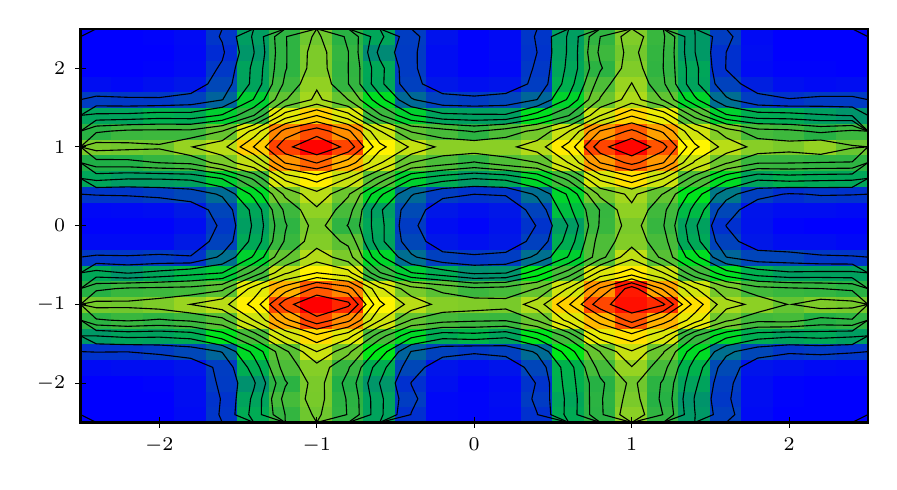
\begin{tikzpicture}
\begin{scope}[]
\pgfpathmoveto{ \pgfpointxy {0.0} {0.0}}
\pgfpathlineto{ \pgfpointxy {10.0} {0.0}}
\pgfpathlineto{ \pgfpointxy {10.0} {5.0}}
\pgfpathlineto{ \pgfpointxy {0.0} {5.0}}
\pgfpathclose
\pgfusepath{  clip, }
\begin{scope}[shift={(0.0,0.0)}]
\pgfsetxvec{\pgfpoint{2.0cm}{0cm}}
\pgfsetyvec{\pgfpoint{0cm}{1.0cm}}
\begin{scope}[shift={(2.5,2.5)}]
\begin{scope}[green!0!blue]
\pgfpathmoveto{ \pgfpointxy {-2.5} {-2.5}}
\pgfpathlineto{ \pgfpointxy {-2.3} {-2.5}}
\pgfpathlineto{ \pgfpointxy {-2.3} {-2.3}}
\pgfpathlineto{ \pgfpointxy {-2.5} {-2.3}}
\pgfpathclose
\pgfusepath{ stroke, fill, }
\end{scope}
\begin{scope}[green!0!blue]
\pgfpathmoveto{ \pgfpointxy {-2.3} {-2.5}}
\pgfpathlineto{ \pgfpointxy {-2.1} {-2.5}}
\pgfpathlineto{ \pgfpointxy {-2.1} {-2.3}}
\pgfpathlineto{ \pgfpointxy {-2.3} {-2.3}}
\pgfpathclose
\pgfusepath{ stroke, fill, }
\end{scope}
\begin{scope}[green!0!blue]
\pgfpathmoveto{ \pgfpointxy {-2.1} {-2.5}}
\pgfpathlineto{ \pgfpointxy {-1.8999999} {-2.5}}
\pgfpathlineto{ \pgfpointxy {-1.8999999} {-2.3}}
\pgfpathlineto{ \pgfpointxy {-2.1} {-2.3}}
\pgfpathclose
\pgfusepath{ stroke, fill, }
\end{scope}
\begin{scope}[green!4!blue]
\pgfpathmoveto{ \pgfpointxy {-1.9} {-2.5}}
\pgfpathlineto{ \pgfpointxy {-1.6999999} {-2.5}}
\pgfpathlineto{ \pgfpointxy {-1.6999999} {-2.3}}
\pgfpathlineto{ \pgfpointxy {-1.9} {-2.3}}
\pgfpathclose
\pgfusepath{ stroke, fill, }
\end{scope}
\begin{scope}[green!21!blue]
\pgfpathmoveto{ \pgfpointxy {-1.7} {-2.5}}
\pgfpathlineto{ \pgfpointxy {-1.5} {-2.5}}
\pgfpathlineto{ \pgfpointxy {-1.5} {-2.3}}
\pgfpathlineto{ \pgfpointxy {-1.7} {-2.3}}
\pgfpathclose
\pgfusepath{ stroke, fill, }
\end{scope}
\begin{scope}[green!67!blue]
\pgfpathmoveto{ \pgfpointxy {-1.5} {-2.5}}
\pgfpathlineto{ \pgfpointxy {-1.3} {-2.5}}
\pgfpathlineto{ \pgfpointxy {-1.3} {-2.3}}
\pgfpathlineto{ \pgfpointxy {-1.5} {-2.3}}
\pgfpathclose
\pgfusepath{ stroke, fill, }
\end{scope}
\begin{scope}[yellow!20!green]
\pgfpathmoveto{ \pgfpointxy {-1.3} {-2.5}}
\pgfpathlineto{ \pgfpointxy {-1.0999999} {-2.5}}
\pgfpathlineto{ \pgfpointxy {-1.0999999} {-2.3}}
\pgfpathlineto{ \pgfpointxy {-1.3} {-2.3}}
\pgfpathclose
\pgfusepath{ stroke, fill, }
\end{scope}
\begin{scope}[yellow!43!green]
\pgfpathmoveto{ \pgfpointxy {-1.1} {-2.5}}
\pgfpathlineto{ \pgfpointxy {-0.90000004} {-2.5}}
\pgfpathlineto{ \pgfpointxy {-0.90000004} {-2.3}}
\pgfpathlineto{ \pgfpointxy {-1.1} {-2.3}}
\pgfpathclose
\pgfusepath{ stroke, fill, }
\end{scope}
\begin{scope}[yellow!18!green]
\pgfpathmoveto{ \pgfpointxy {-0.9} {-2.5}}
\pgfpathlineto{ \pgfpointxy {-0.7} {-2.5}}
\pgfpathlineto{ \pgfpointxy {-0.7} {-2.3}}
\pgfpathlineto{ \pgfpointxy {-0.9} {-2.3}}
\pgfpathclose
\pgfusepath{ stroke, fill, }
\end{scope}
\begin{scope}[green!64!blue]
\pgfpathmoveto{ \pgfpointxy {-0.6999999} {-2.5}}
\pgfpathlineto{ \pgfpointxy {-0.49999994} {-2.5}}
\pgfpathlineto{ \pgfpointxy {-0.49999994} {-2.3}}
\pgfpathlineto{ \pgfpointxy {-0.6999999} {-2.3}}
\pgfpathclose
\pgfusepath{ stroke, fill, }
\end{scope}
\begin{scope}[green!19!blue]
\pgfpathmoveto{ \pgfpointxy {-0.5} {-2.5}}
\pgfpathlineto{ \pgfpointxy {-0.3} {-2.5}}
\pgfpathlineto{ \pgfpointxy {-0.3} {-2.3}}
\pgfpathlineto{ \pgfpointxy {-0.5} {-2.3}}
\pgfpathclose
\pgfusepath{ stroke, fill, }
\end{scope}
\begin{scope}[green!3!blue]
\pgfpathmoveto{ \pgfpointxy {-0.29999995} {-2.5}}
\pgfpathlineto{ \pgfpointxy {-0.09999995} {-2.5}}
\pgfpathlineto{ \pgfpointxy {-0.09999995} {-2.3}}
\pgfpathlineto{ \pgfpointxy {-0.29999995} {-2.3}}
\pgfpathclose
\pgfusepath{ stroke, fill, }
\end{scope}
\begin{scope}[green!2!blue]
\pgfpathmoveto{ \pgfpointxy {-0.099999905} {-2.5}}
\pgfpathlineto{ \pgfpointxy {0.1000001} {-2.5}}
\pgfpathlineto{ \pgfpointxy {0.1000001} {-2.3}}
\pgfpathlineto{ \pgfpointxy {-0.099999905} {-2.3}}
\pgfpathclose
\pgfusepath{ stroke, fill, }
\end{scope}
\begin{scope}[green!4!blue]
\pgfpathmoveto{ \pgfpointxy {0.10000014} {-2.5}}
\pgfpathlineto{ \pgfpointxy {0.30000013} {-2.5}}
\pgfpathlineto{ \pgfpointxy {0.30000013} {-2.3}}
\pgfpathlineto{ \pgfpointxy {0.10000014} {-2.3}}
\pgfpathclose
\pgfusepath{ stroke, fill, }
\end{scope}
\begin{scope}[green!19!blue]
\pgfpathmoveto{ \pgfpointxy {0.29999995} {-2.5}}
\pgfpathlineto{ \pgfpointxy {0.49999994} {-2.5}}
\pgfpathlineto{ \pgfpointxy {0.49999994} {-2.3}}
\pgfpathlineto{ \pgfpointxy {0.29999995} {-2.3}}
\pgfpathclose
\pgfusepath{ stroke, fill, }
\end{scope}
\begin{scope}[green!67!blue]
\pgfpathmoveto{ \pgfpointxy {0.5} {-2.5}}
\pgfpathlineto{ \pgfpointxy {0.7} {-2.5}}
\pgfpathlineto{ \pgfpointxy {0.7} {-2.3}}
\pgfpathlineto{ \pgfpointxy {0.5} {-2.3}}
\pgfpathclose
\pgfusepath{ stroke, fill, }
\end{scope}
\begin{scope}[yellow!16!green]
\pgfpathmoveto{ \pgfpointxy {0.70000005} {-2.5}}
\pgfpathlineto{ \pgfpointxy {0.90000004} {-2.5}}
\pgfpathlineto{ \pgfpointxy {0.90000004} {-2.3}}
\pgfpathlineto{ \pgfpointxy {0.70000005} {-2.3}}
\pgfpathclose
\pgfusepath{ stroke, fill, }
\end{scope}
\begin{scope}[yellow!54!green]
\pgfpathmoveto{ \pgfpointxy {0.9000001} {-2.5}}
\pgfpathlineto{ \pgfpointxy {1.1000001} {-2.5}}
\pgfpathlineto{ \pgfpointxy {1.1000001} {-2.3}}
\pgfpathlineto{ \pgfpointxy {0.9000001} {-2.3}}
\pgfpathclose
\pgfusepath{ stroke, fill, }
\end{scope}
\begin{scope}[yellow!19!green]
\pgfpathmoveto{ \pgfpointxy {1.1000001} {-2.5}}
\pgfpathlineto{ \pgfpointxy {1.3000002} {-2.5}}
\pgfpathlineto{ \pgfpointxy {1.3000002} {-2.3}}
\pgfpathlineto{ \pgfpointxy {1.1000001} {-2.3}}
\pgfpathclose
\pgfusepath{ stroke, fill, }
\end{scope}
\begin{scope}[green!60!blue]
\pgfpathmoveto{ \pgfpointxy {1.3} {-2.5}}
\pgfpathlineto{ \pgfpointxy {1.5} {-2.5}}
\pgfpathlineto{ \pgfpointxy {1.5} {-2.3}}
\pgfpathlineto{ \pgfpointxy {1.3} {-2.3}}
\pgfpathclose
\pgfusepath{ stroke, fill, }
\end{scope}
\begin{scope}[green!25!blue]
\pgfpathmoveto{ \pgfpointxy {1.5} {-2.5}}
\pgfpathlineto{ \pgfpointxy {1.7} {-2.5}}
\pgfpathlineto{ \pgfpointxy {1.7} {-2.3}}
\pgfpathlineto{ \pgfpointxy {1.5} {-2.3}}
\pgfpathclose
\pgfusepath{ stroke, fill, }
\end{scope}
\begin{scope}[green!4!blue]
\pgfpathmoveto{ \pgfpointxy {1.7000003} {-2.5}}
\pgfpathlineto{ \pgfpointxy {1.9000003} {-2.5}}
\pgfpathlineto{ \pgfpointxy {1.9000003} {-2.3}}
\pgfpathlineto{ \pgfpointxy {1.7000003} {-2.3}}
\pgfpathclose
\pgfusepath{ stroke, fill, }
\end{scope}
\begin{scope}[green!0!blue]
\pgfpathmoveto{ \pgfpointxy {1.9000001} {-2.5}}
\pgfpathlineto{ \pgfpointxy {2.1000001} {-2.5}}
\pgfpathlineto{ \pgfpointxy {2.1000001} {-2.3}}
\pgfpathlineto{ \pgfpointxy {1.9000001} {-2.3}}
\pgfpathclose
\pgfusepath{ stroke, fill, }
\end{scope}
\begin{scope}[green!0!blue]
\pgfpathmoveto{ \pgfpointxy {2.1} {-2.5}}
\pgfpathlineto{ \pgfpointxy {2.3} {-2.5}}
\pgfpathlineto{ \pgfpointxy {2.3} {-2.3}}
\pgfpathlineto{ \pgfpointxy {2.1} {-2.3}}
\pgfpathclose
\pgfusepath{ stroke, fill, }
\end{scope}
\begin{scope}[green!0!blue]
\pgfpathmoveto{ \pgfpointxy {2.3000002} {-2.5}}
\pgfpathlineto{ \pgfpointxy {2.5000002} {-2.5}}
\pgfpathlineto{ \pgfpointxy {2.5000002} {-2.3}}
\pgfpathlineto{ \pgfpointxy {2.3000002} {-2.3}}
\pgfpathclose
\pgfusepath{ stroke, fill, }
\end{scope}
\begin{scope}[green!0!blue]
\pgfpathmoveto{ \pgfpointxy {-2.5} {-2.3}}
\pgfpathlineto{ \pgfpointxy {-2.3} {-2.3}}
\pgfpathlineto{ \pgfpointxy {-2.3} {-2.1}}
\pgfpathlineto{ \pgfpointxy {-2.5} {-2.1}}
\pgfpathclose
\pgfusepath{ stroke, fill, }
\end{scope}
\begin{scope}[green!0!blue]
\pgfpathmoveto{ \pgfpointxy {-2.3} {-2.3}}
\pgfpathlineto{ \pgfpointxy {-2.1} {-2.3}}
\pgfpathlineto{ \pgfpointxy {-2.1} {-2.1}}
\pgfpathlineto{ \pgfpointxy {-2.3} {-2.1}}
\pgfpathclose
\pgfusepath{ stroke, fill, }
\end{scope}
\begin{scope}[green!0!blue]
\pgfpathmoveto{ \pgfpointxy {-2.1} {-2.3}}
\pgfpathlineto{ \pgfpointxy {-1.8999999} {-2.3}}
\pgfpathlineto{ \pgfpointxy {-1.8999999} {-2.1}}
\pgfpathlineto{ \pgfpointxy {-2.1} {-2.1}}
\pgfpathclose
\pgfusepath{ stroke, fill, }
\end{scope}
\begin{scope}[green!5!blue]
\pgfpathmoveto{ \pgfpointxy {-1.9} {-2.3}}
\pgfpathlineto{ \pgfpointxy {-1.6999999} {-2.3}}
\pgfpathlineto{ \pgfpointxy {-1.6999999} {-2.1}}
\pgfpathlineto{ \pgfpointxy {-1.9} {-2.1}}
\pgfpathclose
\pgfusepath{ stroke, fill, }
\end{scope}
\begin{scope}[green!20!blue]
\pgfpathmoveto{ \pgfpointxy {-1.7} {-2.3}}
\pgfpathlineto{ \pgfpointxy {-1.5} {-2.3}}
\pgfpathlineto{ \pgfpointxy {-1.5} {-2.1}}
\pgfpathlineto{ \pgfpointxy {-1.7} {-2.1}}
\pgfpathclose
\pgfusepath{ stroke, fill, }
\end{scope}
\begin{scope}[green!64!blue]
\pgfpathmoveto{ \pgfpointxy {-1.5} {-2.3}}
\pgfpathlineto{ \pgfpointxy {-1.3} {-2.3}}
\pgfpathlineto{ \pgfpointxy {-1.3} {-2.1}}
\pgfpathlineto{ \pgfpointxy {-1.5} {-2.1}}
\pgfpathclose
\pgfusepath{ stroke, fill, }
\end{scope}
\begin{scope}[yellow!27!green]
\pgfpathmoveto{ \pgfpointxy {-1.3} {-2.3}}
\pgfpathlineto{ \pgfpointxy {-1.0999999} {-2.3}}
\pgfpathlineto{ \pgfpointxy {-1.0999999} {-2.1}}
\pgfpathlineto{ \pgfpointxy {-1.3} {-2.1}}
\pgfpathclose
\pgfusepath{ stroke, fill, }
\end{scope}
\begin{scope}[yellow!47!green]
\pgfpathmoveto{ \pgfpointxy {-1.1} {-2.3}}
\pgfpathlineto{ \pgfpointxy {-0.90000004} {-2.3}}
\pgfpathlineto{ \pgfpointxy {-0.90000004} {-2.1}}
\pgfpathlineto{ \pgfpointxy {-1.1} {-2.1}}
\pgfpathclose
\pgfusepath{ stroke, fill, }
\end{scope}
\begin{scope}[yellow!17!green]
\pgfpathmoveto{ \pgfpointxy {-0.9} {-2.3}}
\pgfpathlineto{ \pgfpointxy {-0.7} {-2.3}}
\pgfpathlineto{ \pgfpointxy {-0.7} {-2.1}}
\pgfpathlineto{ \pgfpointxy {-0.9} {-2.1}}
\pgfpathclose
\pgfusepath{ stroke, fill, }
\end{scope}
\begin{scope}[green!64!blue]
\pgfpathmoveto{ \pgfpointxy {-0.6999999} {-2.3}}
\pgfpathlineto{ \pgfpointxy {-0.49999994} {-2.3}}
\pgfpathlineto{ \pgfpointxy {-0.49999994} {-2.1}}
\pgfpathlineto{ \pgfpointxy {-0.6999999} {-2.1}}
\pgfpathclose
\pgfusepath{ stroke, fill, }
\end{scope}
\begin{scope}[green!24!blue]
\pgfpathmoveto{ \pgfpointxy {-0.5} {-2.3}}
\pgfpathlineto{ \pgfpointxy {-0.3} {-2.3}}
\pgfpathlineto{ \pgfpointxy {-0.3} {-2.1}}
\pgfpathlineto{ \pgfpointxy {-0.5} {-2.1}}
\pgfpathclose
\pgfusepath{ stroke, fill, }
\end{scope}
\begin{scope}[green!3!blue]
\pgfpathmoveto{ \pgfpointxy {-0.29999995} {-2.3}}
\pgfpathlineto{ \pgfpointxy {-0.09999995} {-2.3}}
\pgfpathlineto{ \pgfpointxy {-0.09999995} {-2.1}}
\pgfpathlineto{ \pgfpointxy {-0.29999995} {-2.1}}
\pgfpathclose
\pgfusepath{ stroke, fill, }
\end{scope}
\begin{scope}[green!2!blue]
\pgfpathmoveto{ \pgfpointxy {-0.099999905} {-2.3}}
\pgfpathlineto{ \pgfpointxy {0.1000001} {-2.3}}
\pgfpathlineto{ \pgfpointxy {0.1000001} {-2.1}}
\pgfpathlineto{ \pgfpointxy {-0.099999905} {-2.1}}
\pgfpathclose
\pgfusepath{ stroke, fill, }
\end{scope}
\begin{scope}[green!5!blue]
\pgfpathmoveto{ \pgfpointxy {0.10000014} {-2.3}}
\pgfpathlineto{ \pgfpointxy {0.30000013} {-2.3}}
\pgfpathlineto{ \pgfpointxy {0.30000013} {-2.1}}
\pgfpathlineto{ \pgfpointxy {0.10000014} {-2.1}}
\pgfpathclose
\pgfusepath{ stroke, fill, }
\end{scope}
\begin{scope}[green!23!blue]
\pgfpathmoveto{ \pgfpointxy {0.29999995} {-2.3}}
\pgfpathlineto{ \pgfpointxy {0.49999994} {-2.3}}
\pgfpathlineto{ \pgfpointxy {0.49999994} {-2.1}}
\pgfpathlineto{ \pgfpointxy {0.29999995} {-2.1}}
\pgfpathclose
\pgfusepath{ stroke, fill, }
\end{scope}
\begin{scope}[green!65!blue]
\pgfpathmoveto{ \pgfpointxy {0.5} {-2.3}}
\pgfpathlineto{ \pgfpointxy {0.7} {-2.3}}
\pgfpathlineto{ \pgfpointxy {0.7} {-2.1}}
\pgfpathlineto{ \pgfpointxy {0.5} {-2.1}}
\pgfpathclose
\pgfusepath{ stroke, fill, }
\end{scope}
\begin{scope}[yellow!17!green]
\pgfpathmoveto{ \pgfpointxy {0.70000005} {-2.3}}
\pgfpathlineto{ \pgfpointxy {0.90000004} {-2.3}}
\pgfpathlineto{ \pgfpointxy {0.90000004} {-2.1}}
\pgfpathlineto{ \pgfpointxy {0.70000005} {-2.1}}
\pgfpathclose
\pgfusepath{ stroke, fill, }
\end{scope}
\begin{scope}[yellow!48!green]
\pgfpathmoveto{ \pgfpointxy {0.9000001} {-2.3}}
\pgfpathlineto{ \pgfpointxy {1.1000001} {-2.3}}
\pgfpathlineto{ \pgfpointxy {1.1000001} {-2.1}}
\pgfpathlineto{ \pgfpointxy {0.9000001} {-2.1}}
\pgfpathclose
\pgfusepath{ stroke, fill, }
\end{scope}
\begin{scope}[yellow!15!green]
\pgfpathmoveto{ \pgfpointxy {1.1000001} {-2.3}}
\pgfpathlineto{ \pgfpointxy {1.3000002} {-2.3}}
\pgfpathlineto{ \pgfpointxy {1.3000002} {-2.1}}
\pgfpathlineto{ \pgfpointxy {1.1000001} {-2.1}}
\pgfpathclose
\pgfusepath{ stroke, fill, }
\end{scope}
\begin{scope}[green!58!blue]
\pgfpathmoveto{ \pgfpointxy {1.3} {-2.3}}
\pgfpathlineto{ \pgfpointxy {1.5} {-2.3}}
\pgfpathlineto{ \pgfpointxy {1.5} {-2.1}}
\pgfpathlineto{ \pgfpointxy {1.3} {-2.1}}
\pgfpathclose
\pgfusepath{ stroke, fill, }
\end{scope}
\begin{scope}[green!22!blue]
\pgfpathmoveto{ \pgfpointxy {1.5} {-2.3}}
\pgfpathlineto{ \pgfpointxy {1.7} {-2.3}}
\pgfpathlineto{ \pgfpointxy {1.7} {-2.1}}
\pgfpathlineto{ \pgfpointxy {1.5} {-2.1}}
\pgfpathclose
\pgfusepath{ stroke, fill, }
\end{scope}
\begin{scope}[green!5!blue]
\pgfpathmoveto{ \pgfpointxy {1.7000003} {-2.3}}
\pgfpathlineto{ \pgfpointxy {1.9000003} {-2.3}}
\pgfpathlineto{ \pgfpointxy {1.9000003} {-2.1}}
\pgfpathlineto{ \pgfpointxy {1.7000003} {-2.1}}
\pgfpathclose
\pgfusepath{ stroke, fill, }
\end{scope}
\begin{scope}[green!1!blue]
\pgfpathmoveto{ \pgfpointxy {1.9000001} {-2.3}}
\pgfpathlineto{ \pgfpointxy {2.1000001} {-2.3}}
\pgfpathlineto{ \pgfpointxy {2.1000001} {-2.1}}
\pgfpathlineto{ \pgfpointxy {1.9000001} {-2.1}}
\pgfpathclose
\pgfusepath{ stroke, fill, }
\end{scope}
\begin{scope}[green!0!blue]
\pgfpathmoveto{ \pgfpointxy {2.1} {-2.3}}
\pgfpathlineto{ \pgfpointxy {2.3} {-2.3}}
\pgfpathlineto{ \pgfpointxy {2.3} {-2.1}}
\pgfpathlineto{ \pgfpointxy {2.1} {-2.1}}
\pgfpathclose
\pgfusepath{ stroke, fill, }
\end{scope}
\begin{scope}[green!0!blue]
\pgfpathmoveto{ \pgfpointxy {2.3000002} {-2.3}}
\pgfpathlineto{ \pgfpointxy {2.5000002} {-2.3}}
\pgfpathlineto{ \pgfpointxy {2.5000002} {-2.1}}
\pgfpathlineto{ \pgfpointxy {2.3000002} {-2.1}}
\pgfpathclose
\pgfusepath{ stroke, fill, }
\end{scope}
\begin{scope}[green!0!blue]
\pgfpathmoveto{ \pgfpointxy {-2.5} {-2.1}}
\pgfpathlineto{ \pgfpointxy {-2.3} {-2.1}}
\pgfpathlineto{ \pgfpointxy {-2.3} {-1.8999999}}
\pgfpathlineto{ \pgfpointxy {-2.5} {-1.8999999}}
\pgfpathclose
\pgfusepath{ stroke, fill, }
\end{scope}
\begin{scope}[green!0!blue]
\pgfpathmoveto{ \pgfpointxy {-2.3} {-2.1}}
\pgfpathlineto{ \pgfpointxy {-2.1} {-2.1}}
\pgfpathlineto{ \pgfpointxy {-2.1} {-1.8999999}}
\pgfpathlineto{ \pgfpointxy {-2.3} {-1.8999999}}
\pgfpathclose
\pgfusepath{ stroke, fill, }
\end{scope}
\begin{scope}[green!1!blue]
\pgfpathmoveto{ \pgfpointxy {-2.1} {-2.1}}
\pgfpathlineto{ \pgfpointxy {-1.8999999} {-2.1}}
\pgfpathlineto{ \pgfpointxy {-1.8999999} {-1.8999999}}
\pgfpathlineto{ \pgfpointxy {-2.1} {-1.8999999}}
\pgfpathclose
\pgfusepath{ stroke, fill, }
\end{scope}
\begin{scope}[green!5!blue]
\pgfpathmoveto{ \pgfpointxy {-1.9} {-2.1}}
\pgfpathlineto{ \pgfpointxy {-1.6999999} {-2.1}}
\pgfpathlineto{ \pgfpointxy {-1.6999999} {-1.8999999}}
\pgfpathlineto{ \pgfpointxy {-1.9} {-1.8999999}}
\pgfpathclose
\pgfusepath{ stroke, fill, }
\end{scope}
\begin{scope}[green!23!blue]
\pgfpathmoveto{ \pgfpointxy {-1.7} {-2.1}}
\pgfpathlineto{ \pgfpointxy {-1.5} {-2.1}}
\pgfpathlineto{ \pgfpointxy {-1.5} {-1.8999999}}
\pgfpathlineto{ \pgfpointxy {-1.7} {-1.8999999}}
\pgfpathclose
\pgfusepath{ stroke, fill, }
\end{scope}
\begin{scope}[green!57!blue]
\pgfpathmoveto{ \pgfpointxy {-1.5} {-2.1}}
\pgfpathlineto{ \pgfpointxy {-1.3} {-2.1}}
\pgfpathlineto{ \pgfpointxy {-1.3} {-1.8999999}}
\pgfpathlineto{ \pgfpointxy {-1.5} {-1.8999999}}
\pgfpathclose
\pgfusepath{ stroke, fill, }
\end{scope}
\begin{scope}[yellow!17!green]
\pgfpathmoveto{ \pgfpointxy {-1.3} {-2.1}}
\pgfpathlineto{ \pgfpointxy {-1.0999999} {-2.1}}
\pgfpathlineto{ \pgfpointxy {-1.0999999} {-1.8999999}}
\pgfpathlineto{ \pgfpointxy {-1.3} {-1.8999999}}
\pgfpathclose
\pgfusepath{ stroke, fill, }
\end{scope}
\begin{scope}[yellow!48!green]
\pgfpathmoveto{ \pgfpointxy {-1.1} {-2.1}}
\pgfpathlineto{ \pgfpointxy {-0.90000004} {-2.1}}
\pgfpathlineto{ \pgfpointxy {-0.90000004} {-1.8999999}}
\pgfpathlineto{ \pgfpointxy {-1.1} {-1.8999999}}
\pgfpathclose
\pgfusepath{ stroke, fill, }
\end{scope}
\begin{scope}[yellow!13!green]
\pgfpathmoveto{ \pgfpointxy {-0.9} {-2.1}}
\pgfpathlineto{ \pgfpointxy {-0.7} {-2.1}}
\pgfpathlineto{ \pgfpointxy {-0.7} {-1.8999999}}
\pgfpathlineto{ \pgfpointxy {-0.9} {-1.8999999}}
\pgfpathclose
\pgfusepath{ stroke, fill, }
\end{scope}
\begin{scope}[green!59!blue]
\pgfpathmoveto{ \pgfpointxy {-0.6999999} {-2.1}}
\pgfpathlineto{ \pgfpointxy {-0.49999994} {-2.1}}
\pgfpathlineto{ \pgfpointxy {-0.49999994} {-1.8999999}}
\pgfpathlineto{ \pgfpointxy {-0.6999999} {-1.8999999}}
\pgfpathclose
\pgfusepath{ stroke, fill, }
\end{scope}
\begin{scope}[green!19!blue]
\pgfpathmoveto{ \pgfpointxy {-0.5} {-2.1}}
\pgfpathlineto{ \pgfpointxy {-0.3} {-2.1}}
\pgfpathlineto{ \pgfpointxy {-0.3} {-1.8999999}}
\pgfpathlineto{ \pgfpointxy {-0.5} {-1.8999999}}
\pgfpathclose
\pgfusepath{ stroke, fill, }
\end{scope}
\begin{scope}[green!6!blue]
\pgfpathmoveto{ \pgfpointxy {-0.29999995} {-2.1}}
\pgfpathlineto{ \pgfpointxy {-0.09999995} {-2.1}}
\pgfpathlineto{ \pgfpointxy {-0.09999995} {-1.8999999}}
\pgfpathlineto{ \pgfpointxy {-0.29999995} {-1.8999999}}
\pgfpathclose
\pgfusepath{ stroke, fill, }
\end{scope}
\begin{scope}[green!1!blue]
\pgfpathmoveto{ \pgfpointxy {-0.099999905} {-2.1}}
\pgfpathlineto{ \pgfpointxy {0.1000001} {-2.1}}
\pgfpathlineto{ \pgfpointxy {0.1000001} {-1.8999999}}
\pgfpathlineto{ \pgfpointxy {-0.099999905} {-1.8999999}}
\pgfpathclose
\pgfusepath{ stroke, fill, }
\end{scope}
\begin{scope}[green!4!blue]
\pgfpathmoveto{ \pgfpointxy {0.10000014} {-2.1}}
\pgfpathlineto{ \pgfpointxy {0.30000013} {-2.1}}
\pgfpathlineto{ \pgfpointxy {0.30000013} {-1.8999999}}
\pgfpathlineto{ \pgfpointxy {0.10000014} {-1.8999999}}
\pgfpathclose
\pgfusepath{ stroke, fill, }
\end{scope}
\begin{scope}[green!20!blue]
\pgfpathmoveto{ \pgfpointxy {0.29999995} {-2.1}}
\pgfpathlineto{ \pgfpointxy {0.49999994} {-2.1}}
\pgfpathlineto{ \pgfpointxy {0.49999994} {-1.8999999}}
\pgfpathlineto{ \pgfpointxy {0.29999995} {-1.8999999}}
\pgfpathclose
\pgfusepath{ stroke, fill, }
\end{scope}
\begin{scope}[green!69!blue]
\pgfpathmoveto{ \pgfpointxy {0.5} {-2.1}}
\pgfpathlineto{ \pgfpointxy {0.7} {-2.1}}
\pgfpathlineto{ \pgfpointxy {0.7} {-1.8999999}}
\pgfpathlineto{ \pgfpointxy {0.5} {-1.8999999}}
\pgfpathclose
\pgfusepath{ stroke, fill, }
\end{scope}
\begin{scope}[yellow!15!green]
\pgfpathmoveto{ \pgfpointxy {0.70000005} {-2.1}}
\pgfpathlineto{ \pgfpointxy {0.90000004} {-2.1}}
\pgfpathlineto{ \pgfpointxy {0.90000004} {-1.8999999}}
\pgfpathlineto{ \pgfpointxy {0.70000005} {-1.8999999}}
\pgfpathclose
\pgfusepath{ stroke, fill, }
\end{scope}
\begin{scope}[yellow!44!green]
\pgfpathmoveto{ \pgfpointxy {0.9000001} {-2.1}}
\pgfpathlineto{ \pgfpointxy {1.1000001} {-2.1}}
\pgfpathlineto{ \pgfpointxy {1.1000001} {-1.8999999}}
\pgfpathlineto{ \pgfpointxy {0.9000001} {-1.8999999}}
\pgfpathclose
\pgfusepath{ stroke, fill, }
\end{scope}
\begin{scope}[yellow!17!green]
\pgfpathmoveto{ \pgfpointxy {1.1000001} {-2.1}}
\pgfpathlineto{ \pgfpointxy {1.3000002} {-2.1}}
\pgfpathlineto{ \pgfpointxy {1.3000002} {-1.8999999}}
\pgfpathlineto{ \pgfpointxy {1.1000001} {-1.8999999}}
\pgfpathclose
\pgfusepath{ stroke, fill, }
\end{scope}
\begin{scope}[green!64!blue]
\pgfpathmoveto{ \pgfpointxy {1.3} {-2.1}}
\pgfpathlineto{ \pgfpointxy {1.5} {-2.1}}
\pgfpathlineto{ \pgfpointxy {1.5} {-1.8999999}}
\pgfpathlineto{ \pgfpointxy {1.3} {-1.8999999}}
\pgfpathclose
\pgfusepath{ stroke, fill, }
\end{scope}
\begin{scope}[green!24!blue]
\pgfpathmoveto{ \pgfpointxy {1.5} {-2.1}}
\pgfpathlineto{ \pgfpointxy {1.7} {-2.1}}
\pgfpathlineto{ \pgfpointxy {1.7} {-1.8999999}}
\pgfpathlineto{ \pgfpointxy {1.5} {-1.8999999}}
\pgfpathclose
\pgfusepath{ stroke, fill, }
\end{scope}
\begin{scope}[green!5!blue]
\pgfpathmoveto{ \pgfpointxy {1.7000003} {-2.1}}
\pgfpathlineto{ \pgfpointxy {1.9000003} {-2.1}}
\pgfpathlineto{ \pgfpointxy {1.9000003} {-1.8999999}}
\pgfpathlineto{ \pgfpointxy {1.7000003} {-1.8999999}}
\pgfpathclose
\pgfusepath{ stroke, fill, }
\end{scope}
\begin{scope}[green!1!blue]
\pgfpathmoveto{ \pgfpointxy {1.9000001} {-2.1}}
\pgfpathlineto{ \pgfpointxy {2.1000001} {-2.1}}
\pgfpathlineto{ \pgfpointxy {2.1000001} {-1.8999999}}
\pgfpathlineto{ \pgfpointxy {1.9000001} {-1.8999999}}
\pgfpathclose
\pgfusepath{ stroke, fill, }
\end{scope}
\begin{scope}[green!0!blue]
\pgfpathmoveto{ \pgfpointxy {2.1} {-2.1}}
\pgfpathlineto{ \pgfpointxy {2.3} {-2.1}}
\pgfpathlineto{ \pgfpointxy {2.3} {-1.8999999}}
\pgfpathlineto{ \pgfpointxy {2.1} {-1.8999999}}
\pgfpathclose
\pgfusepath{ stroke, fill, }
\end{scope}
\begin{scope}[green!0!blue]
\pgfpathmoveto{ \pgfpointxy {2.3000002} {-2.1}}
\pgfpathlineto{ \pgfpointxy {2.5000002} {-2.1}}
\pgfpathlineto{ \pgfpointxy {2.5000002} {-1.8999999}}
\pgfpathlineto{ \pgfpointxy {2.3000002} {-1.8999999}}
\pgfpathclose
\pgfusepath{ stroke, fill, }
\end{scope}
\begin{scope}[green!4!blue]
\pgfpathmoveto{ \pgfpointxy {-2.5} {-1.9}}
\pgfpathlineto{ \pgfpointxy {-2.3} {-1.9}}
\pgfpathlineto{ \pgfpointxy {-2.3} {-1.6999999}}
\pgfpathlineto{ \pgfpointxy {-2.5} {-1.6999999}}
\pgfpathclose
\pgfusepath{ stroke, fill, }
\end{scope}
\begin{scope}[green!5!blue]
\pgfpathmoveto{ \pgfpointxy {-2.3} {-1.9}}
\pgfpathlineto{ \pgfpointxy {-2.1} {-1.9}}
\pgfpathlineto{ \pgfpointxy {-2.1} {-1.6999999}}
\pgfpathlineto{ \pgfpointxy {-2.3} {-1.6999999}}
\pgfpathclose
\pgfusepath{ stroke, fill, }
\end{scope}
\begin{scope}[green!5!blue]
\pgfpathmoveto{ \pgfpointxy {-2.1} {-1.9}}
\pgfpathlineto{ \pgfpointxy {-1.8999999} {-1.9}}
\pgfpathlineto{ \pgfpointxy {-1.8999999} {-1.6999999}}
\pgfpathlineto{ \pgfpointxy {-2.1} {-1.6999999}}
\pgfpathclose
\pgfusepath{ stroke, fill, }
\end{scope}
\begin{scope}[green!8!blue]
\pgfpathmoveto{ \pgfpointxy {-1.9} {-1.9}}
\pgfpathlineto{ \pgfpointxy {-1.6999999} {-1.9}}
\pgfpathlineto{ \pgfpointxy {-1.6999999} {-1.6999999}}
\pgfpathlineto{ \pgfpointxy {-1.9} {-1.6999999}}
\pgfpathclose
\pgfusepath{ stroke, fill, }
\end{scope}
\begin{scope}[green!24!blue]
\pgfpathmoveto{ \pgfpointxy {-1.7} {-1.9}}
\pgfpathlineto{ \pgfpointxy {-1.5} {-1.9}}
\pgfpathlineto{ \pgfpointxy {-1.5} {-1.6999999}}
\pgfpathlineto{ \pgfpointxy {-1.7} {-1.6999999}}
\pgfpathclose
\pgfusepath{ stroke, fill, }
\end{scope}
\begin{scope}[green!68!blue]
\pgfpathmoveto{ \pgfpointxy {-1.5} {-1.9}}
\pgfpathlineto{ \pgfpointxy {-1.3} {-1.9}}
\pgfpathlineto{ \pgfpointxy {-1.3} {-1.6999999}}
\pgfpathlineto{ \pgfpointxy {-1.5} {-1.6999999}}
\pgfpathclose
\pgfusepath{ stroke, fill, }
\end{scope}
\begin{scope}[yellow!30!green]
\pgfpathmoveto{ \pgfpointxy {-1.3} {-1.9}}
\pgfpathlineto{ \pgfpointxy {-1.0999999} {-1.9}}
\pgfpathlineto{ \pgfpointxy {-1.0999999} {-1.6999999}}
\pgfpathlineto{ \pgfpointxy {-1.3} {-1.6999999}}
\pgfpathclose
\pgfusepath{ stroke, fill, }
\end{scope}
\begin{scope}[yellow!52!green]
\pgfpathmoveto{ \pgfpointxy {-1.1} {-1.9}}
\pgfpathlineto{ \pgfpointxy {-0.90000004} {-1.9}}
\pgfpathlineto{ \pgfpointxy {-0.90000004} {-1.6999999}}
\pgfpathlineto{ \pgfpointxy {-1.1} {-1.6999999}}
\pgfpathclose
\pgfusepath{ stroke, fill, }
\end{scope}
\begin{scope}[yellow!21!green]
\pgfpathmoveto{ \pgfpointxy {-0.9} {-1.9}}
\pgfpathlineto{ \pgfpointxy {-0.7} {-1.9}}
\pgfpathlineto{ \pgfpointxy {-0.7} {-1.6999999}}
\pgfpathlineto{ \pgfpointxy {-0.9} {-1.6999999}}
\pgfpathclose
\pgfusepath{ stroke, fill, }
\end{scope}
\begin{scope}[green!68!blue]
\pgfpathmoveto{ \pgfpointxy {-0.6999999} {-1.9}}
\pgfpathlineto{ \pgfpointxy {-0.49999994} {-1.9}}
\pgfpathlineto{ \pgfpointxy {-0.49999994} {-1.6999999}}
\pgfpathlineto{ \pgfpointxy {-0.6999999} {-1.6999999}}
\pgfpathclose
\pgfusepath{ stroke, fill, }
\end{scope}
\begin{scope}[green!28!blue]
\pgfpathmoveto{ \pgfpointxy {-0.5} {-1.9}}
\pgfpathlineto{ \pgfpointxy {-0.3} {-1.9}}
\pgfpathlineto{ \pgfpointxy {-0.3} {-1.6999999}}
\pgfpathlineto{ \pgfpointxy {-0.5} {-1.6999999}}
\pgfpathclose
\pgfusepath{ stroke, fill, }
\end{scope}
\begin{scope}[green!8!blue]
\pgfpathmoveto{ \pgfpointxy {-0.29999995} {-1.9}}
\pgfpathlineto{ \pgfpointxy {-0.09999995} {-1.9}}
\pgfpathlineto{ \pgfpointxy {-0.09999995} {-1.6999999}}
\pgfpathlineto{ \pgfpointxy {-0.29999995} {-1.6999999}}
\pgfpathclose
\pgfusepath{ stroke, fill, }
\end{scope}
\begin{scope}[green!5!blue]
\pgfpathmoveto{ \pgfpointxy {-0.099999905} {-1.9}}
\pgfpathlineto{ \pgfpointxy {0.1000001} {-1.9}}
\pgfpathlineto{ \pgfpointxy {0.1000001} {-1.6999999}}
\pgfpathlineto{ \pgfpointxy {-0.099999905} {-1.6999999}}
\pgfpathclose
\pgfusepath{ stroke, fill, }
\end{scope}
\begin{scope}[green!8!blue]
\pgfpathmoveto{ \pgfpointxy {0.10000014} {-1.9}}
\pgfpathlineto{ \pgfpointxy {0.30000013} {-1.9}}
\pgfpathlineto{ \pgfpointxy {0.30000013} {-1.6999999}}
\pgfpathlineto{ \pgfpointxy {0.10000014} {-1.6999999}}
\pgfpathclose
\pgfusepath{ stroke, fill, }
\end{scope}
\begin{scope}[green!27!blue]
\pgfpathmoveto{ \pgfpointxy {0.29999995} {-1.9}}
\pgfpathlineto{ \pgfpointxy {0.49999994} {-1.9}}
\pgfpathlineto{ \pgfpointxy {0.49999994} {-1.6999999}}
\pgfpathlineto{ \pgfpointxy {0.29999995} {-1.6999999}}
\pgfpathclose
\pgfusepath{ stroke, fill, }
\end{scope}
\begin{scope}[green!70!blue]
\pgfpathmoveto{ \pgfpointxy {0.5} {-1.9}}
\pgfpathlineto{ \pgfpointxy {0.7} {-1.9}}
\pgfpathlineto{ \pgfpointxy {0.7} {-1.6999999}}
\pgfpathlineto{ \pgfpointxy {0.5} {-1.6999999}}
\pgfpathclose
\pgfusepath{ stroke, fill, }
\end{scope}
\begin{scope}[yellow!27!green]
\pgfpathmoveto{ \pgfpointxy {0.70000005} {-1.9}}
\pgfpathlineto{ \pgfpointxy {0.90000004} {-1.9}}
\pgfpathlineto{ \pgfpointxy {0.90000004} {-1.6999999}}
\pgfpathlineto{ \pgfpointxy {0.70000005} {-1.6999999}}
\pgfpathclose
\pgfusepath{ stroke, fill, }
\end{scope}
\begin{scope}[yellow!59!green]
\pgfpathmoveto{ \pgfpointxy {0.9000001} {-1.9}}
\pgfpathlineto{ \pgfpointxy {1.1000001} {-1.9}}
\pgfpathlineto{ \pgfpointxy {1.1000001} {-1.6999999}}
\pgfpathlineto{ \pgfpointxy {0.9000001} {-1.6999999}}
\pgfpathclose
\pgfusepath{ stroke, fill, }
\end{scope}
\begin{scope}[yellow!27!green]
\pgfpathmoveto{ \pgfpointxy {1.1000001} {-1.9}}
\pgfpathlineto{ \pgfpointxy {1.3000002} {-1.9}}
\pgfpathlineto{ \pgfpointxy {1.3000002} {-1.6999999}}
\pgfpathlineto{ \pgfpointxy {1.1000001} {-1.6999999}}
\pgfpathclose
\pgfusepath{ stroke, fill, }
\end{scope}
\begin{scope}[green!70!blue]
\pgfpathmoveto{ \pgfpointxy {1.3} {-1.9}}
\pgfpathlineto{ \pgfpointxy {1.5} {-1.9}}
\pgfpathlineto{ \pgfpointxy {1.5} {-1.6999999}}
\pgfpathlineto{ \pgfpointxy {1.3} {-1.6999999}}
\pgfpathclose
\pgfusepath{ stroke, fill, }
\end{scope}
\begin{scope}[green!29!blue]
\pgfpathmoveto{ \pgfpointxy {1.5} {-1.9}}
\pgfpathlineto{ \pgfpointxy {1.7} {-1.9}}
\pgfpathlineto{ \pgfpointxy {1.7} {-1.6999999}}
\pgfpathlineto{ \pgfpointxy {1.5} {-1.6999999}}
\pgfpathclose
\pgfusepath{ stroke, fill, }
\end{scope}
\begin{scope}[green!8!blue]
\pgfpathmoveto{ \pgfpointxy {1.7000003} {-1.9}}
\pgfpathlineto{ \pgfpointxy {1.9000003} {-1.9}}
\pgfpathlineto{ \pgfpointxy {1.9000003} {-1.6999999}}
\pgfpathlineto{ \pgfpointxy {1.7000003} {-1.6999999}}
\pgfpathclose
\pgfusepath{ stroke, fill, }
\end{scope}
\begin{scope}[green!6!blue]
\pgfpathmoveto{ \pgfpointxy {1.9000001} {-1.9}}
\pgfpathlineto{ \pgfpointxy {2.1000001} {-1.9}}
\pgfpathlineto{ \pgfpointxy {2.1000001} {-1.6999999}}
\pgfpathlineto{ \pgfpointxy {1.9000001} {-1.6999999}}
\pgfpathclose
\pgfusepath{ stroke, fill, }
\end{scope}
\begin{scope}[green!4!blue]
\pgfpathmoveto{ \pgfpointxy {2.1} {-1.9}}
\pgfpathlineto{ \pgfpointxy {2.3} {-1.9}}
\pgfpathlineto{ \pgfpointxy {2.3} {-1.6999999}}
\pgfpathlineto{ \pgfpointxy {2.1} {-1.6999999}}
\pgfpathclose
\pgfusepath{ stroke, fill, }
\end{scope}
\begin{scope}[green!3!blue]
\pgfpathmoveto{ \pgfpointxy {2.3000002} {-1.9}}
\pgfpathlineto{ \pgfpointxy {2.5000002} {-1.9}}
\pgfpathlineto{ \pgfpointxy {2.5000002} {-1.6999999}}
\pgfpathlineto{ \pgfpointxy {2.3000002} {-1.6999999}}
\pgfpathclose
\pgfusepath{ stroke, fill, }
\end{scope}
\begin{scope}[green!20!blue]
\pgfpathmoveto{ \pgfpointxy {-2.5} {-1.7}}
\pgfpathlineto{ \pgfpointxy {-2.3} {-1.7}}
\pgfpathlineto{ \pgfpointxy {-2.3} {-1.5}}
\pgfpathlineto{ \pgfpointxy {-2.5} {-1.5}}
\pgfpathclose
\pgfusepath{ stroke, fill, }
\end{scope}
\begin{scope}[green!20!blue]
\pgfpathmoveto{ \pgfpointxy {-2.3} {-1.7}}
\pgfpathlineto{ \pgfpointxy {-2.1} {-1.7}}
\pgfpathlineto{ \pgfpointxy {-2.1} {-1.5}}
\pgfpathlineto{ \pgfpointxy {-2.3} {-1.5}}
\pgfpathclose
\pgfusepath{ stroke, fill, }
\end{scope}
\begin{scope}[green!23!blue]
\pgfpathmoveto{ \pgfpointxy {-2.1} {-1.7}}
\pgfpathlineto{ \pgfpointxy {-1.8999999} {-1.7}}
\pgfpathlineto{ \pgfpointxy {-1.8999999} {-1.5}}
\pgfpathlineto{ \pgfpointxy {-2.1} {-1.5}}
\pgfpathclose
\pgfusepath{ stroke, fill, }
\end{scope}
\begin{scope}[green!28!blue]
\pgfpathmoveto{ \pgfpointxy {-1.9} {-1.7}}
\pgfpathlineto{ \pgfpointxy {-1.6999999} {-1.7}}
\pgfpathlineto{ \pgfpointxy {-1.6999999} {-1.5}}
\pgfpathlineto{ \pgfpointxy {-1.9} {-1.5}}
\pgfpathclose
\pgfusepath{ stroke, fill, }
\end{scope}
\begin{scope}[green!40!blue]
\pgfpathmoveto{ \pgfpointxy {-1.7} {-1.7}}
\pgfpathlineto{ \pgfpointxy {-1.5} {-1.7}}
\pgfpathlineto{ \pgfpointxy {-1.5} {-1.5}}
\pgfpathlineto{ \pgfpointxy {-1.7} {-1.5}}
\pgfpathclose
\pgfusepath{ stroke, fill, }
\end{scope}
\begin{scope}[green!85!blue]
\pgfpathmoveto{ \pgfpointxy {-1.5} {-1.7}}
\pgfpathlineto{ \pgfpointxy {-1.3} {-1.7}}
\pgfpathlineto{ \pgfpointxy {-1.3} {-1.5}}
\pgfpathlineto{ \pgfpointxy {-1.5} {-1.5}}
\pgfpathclose
\pgfusepath{ stroke, fill, }
\end{scope}
\begin{scope}[yellow!35!green]
\pgfpathmoveto{ \pgfpointxy {-1.3} {-1.7}}
\pgfpathlineto{ \pgfpointxy {-1.0999999} {-1.7}}
\pgfpathlineto{ \pgfpointxy {-1.0999999} {-1.5}}
\pgfpathlineto{ \pgfpointxy {-1.3} {-1.5}}
\pgfpathclose
\pgfusepath{ stroke, fill, }
\end{scope}
\begin{scope}[yellow!80!green]
\pgfpathmoveto{ \pgfpointxy {-1.1} {-1.7}}
\pgfpathlineto{ \pgfpointxy {-0.90000004} {-1.7}}
\pgfpathlineto{ \pgfpointxy {-0.90000004} {-1.5}}
\pgfpathlineto{ \pgfpointxy {-1.1} {-1.5}}
\pgfpathclose
\pgfusepath{ stroke, fill, }
\end{scope}
\begin{scope}[yellow!44!green]
\pgfpathmoveto{ \pgfpointxy {-0.9} {-1.7}}
\pgfpathlineto{ \pgfpointxy {-0.7} {-1.7}}
\pgfpathlineto{ \pgfpointxy {-0.7} {-1.5}}
\pgfpathlineto{ \pgfpointxy {-0.9} {-1.5}}
\pgfpathclose
\pgfusepath{ stroke, fill, }
\end{scope}
\begin{scope}[green!91!blue]
\pgfpathmoveto{ \pgfpointxy {-0.6999999} {-1.7}}
\pgfpathlineto{ \pgfpointxy {-0.49999994} {-1.7}}
\pgfpathlineto{ \pgfpointxy {-0.49999994} {-1.5}}
\pgfpathlineto{ \pgfpointxy {-0.6999999} {-1.5}}
\pgfpathclose
\pgfusepath{ stroke, fill, }
\end{scope}
\begin{scope}[green!39!blue]
\pgfpathmoveto{ \pgfpointxy {-0.5} {-1.7}}
\pgfpathlineto{ \pgfpointxy {-0.3} {-1.7}}
\pgfpathlineto{ \pgfpointxy {-0.3} {-1.5}}
\pgfpathlineto{ \pgfpointxy {-0.5} {-1.5}}
\pgfpathclose
\pgfusepath{ stroke, fill, }
\end{scope}
\begin{scope}[green!26!blue]
\pgfpathmoveto{ \pgfpointxy {-0.29999995} {-1.7}}
\pgfpathlineto{ \pgfpointxy {-0.09999995} {-1.7}}
\pgfpathlineto{ \pgfpointxy {-0.09999995} {-1.5}}
\pgfpathlineto{ \pgfpointxy {-0.29999995} {-1.5}}
\pgfpathclose
\pgfusepath{ stroke, fill, }
\end{scope}
\begin{scope}[green!22!blue]
\pgfpathmoveto{ \pgfpointxy {-0.099999905} {-1.7}}
\pgfpathlineto{ \pgfpointxy {0.1000001} {-1.7}}
\pgfpathlineto{ \pgfpointxy {0.1000001} {-1.5}}
\pgfpathlineto{ \pgfpointxy {-0.099999905} {-1.5}}
\pgfpathclose
\pgfusepath{ stroke, fill, }
\end{scope}
\begin{scope}[green!25!blue]
\pgfpathmoveto{ \pgfpointxy {0.10000014} {-1.7}}
\pgfpathlineto{ \pgfpointxy {0.30000013} {-1.7}}
\pgfpathlineto{ \pgfpointxy {0.30000013} {-1.5}}
\pgfpathlineto{ \pgfpointxy {0.10000014} {-1.5}}
\pgfpathclose
\pgfusepath{ stroke, fill, }
\end{scope}
\begin{scope}[green!42!blue]
\pgfpathmoveto{ \pgfpointxy {0.29999995} {-1.7}}
\pgfpathlineto{ \pgfpointxy {0.49999994} {-1.7}}
\pgfpathlineto{ \pgfpointxy {0.49999994} {-1.5}}
\pgfpathlineto{ \pgfpointxy {0.29999995} {-1.5}}
\pgfpathclose
\pgfusepath{ stroke, fill, }
\end{scope}
\begin{scope}[green!91!blue]
\pgfpathmoveto{ \pgfpointxy {0.5} {-1.7}}
\pgfpathlineto{ \pgfpointxy {0.7} {-1.7}}
\pgfpathlineto{ \pgfpointxy {0.7} {-1.5}}
\pgfpathlineto{ \pgfpointxy {0.5} {-1.5}}
\pgfpathclose
\pgfusepath{ stroke, fill, }
\end{scope}
\begin{scope}[yellow!40!green]
\pgfpathmoveto{ \pgfpointxy {0.70000005} {-1.7}}
\pgfpathlineto{ \pgfpointxy {0.90000004} {-1.7}}
\pgfpathlineto{ \pgfpointxy {0.90000004} {-1.5}}
\pgfpathlineto{ \pgfpointxy {0.70000005} {-1.5}}
\pgfpathclose
\pgfusepath{ stroke, fill, }
\end{scope}
\begin{scope}[yellow!78!green]
\pgfpathmoveto{ \pgfpointxy {0.9000001} {-1.7}}
\pgfpathlineto{ \pgfpointxy {1.1000001} {-1.7}}
\pgfpathlineto{ \pgfpointxy {1.1000001} {-1.5}}
\pgfpathlineto{ \pgfpointxy {0.9000001} {-1.5}}
\pgfpathclose
\pgfusepath{ stroke, fill, }
\end{scope}
\begin{scope}[yellow!41!green]
\pgfpathmoveto{ \pgfpointxy {1.1000001} {-1.7}}
\pgfpathlineto{ \pgfpointxy {1.3000002} {-1.7}}
\pgfpathlineto{ \pgfpointxy {1.3000002} {-1.5}}
\pgfpathlineto{ \pgfpointxy {1.1000001} {-1.5}}
\pgfpathclose
\pgfusepath{ stroke, fill, }
\end{scope}
\begin{scope}[green!86!blue]
\pgfpathmoveto{ \pgfpointxy {1.3} {-1.7}}
\pgfpathlineto{ \pgfpointxy {1.5} {-1.7}}
\pgfpathlineto{ \pgfpointxy {1.5} {-1.5}}
\pgfpathlineto{ \pgfpointxy {1.3} {-1.5}}
\pgfpathclose
\pgfusepath{ stroke, fill, }
\end{scope}
\begin{scope}[green!44!blue]
\pgfpathmoveto{ \pgfpointxy {1.5} {-1.7}}
\pgfpathlineto{ \pgfpointxy {1.7} {-1.7}}
\pgfpathlineto{ \pgfpointxy {1.7} {-1.5}}
\pgfpathlineto{ \pgfpointxy {1.5} {-1.5}}
\pgfpathclose
\pgfusepath{ stroke, fill, }
\end{scope}
\begin{scope}[green!28!blue]
\pgfpathmoveto{ \pgfpointxy {1.7000003} {-1.7}}
\pgfpathlineto{ \pgfpointxy {1.9000003} {-1.7}}
\pgfpathlineto{ \pgfpointxy {1.9000003} {-1.5}}
\pgfpathlineto{ \pgfpointxy {1.7000003} {-1.5}}
\pgfpathclose
\pgfusepath{ stroke, fill, }
\end{scope}
\begin{scope}[green!21!blue]
\pgfpathmoveto{ \pgfpointxy {1.9000001} {-1.7}}
\pgfpathlineto{ \pgfpointxy {2.1000001} {-1.7}}
\pgfpathlineto{ \pgfpointxy {2.1000001} {-1.5}}
\pgfpathlineto{ \pgfpointxy {1.9000001} {-1.5}}
\pgfpathclose
\pgfusepath{ stroke, fill, }
\end{scope}
\begin{scope}[green!23!blue]
\pgfpathmoveto{ \pgfpointxy {2.1} {-1.7}}
\pgfpathlineto{ \pgfpointxy {2.3} {-1.7}}
\pgfpathlineto{ \pgfpointxy {2.3} {-1.5}}
\pgfpathlineto{ \pgfpointxy {2.1} {-1.5}}
\pgfpathclose
\pgfusepath{ stroke, fill, }
\end{scope}
\begin{scope}[green!21!blue]
\pgfpathmoveto{ \pgfpointxy {2.3000002} {-1.7}}
\pgfpathlineto{ \pgfpointxy {2.5000002} {-1.7}}
\pgfpathlineto{ \pgfpointxy {2.5000002} {-1.5}}
\pgfpathlineto{ \pgfpointxy {2.3000002} {-1.5}}
\pgfpathclose
\pgfusepath{ stroke, fill, }
\end{scope}
\begin{scope}[green!60!blue]
\pgfpathmoveto{ \pgfpointxy {-2.5} {-1.5}}
\pgfpathlineto{ \pgfpointxy {-2.3} {-1.5}}
\pgfpathlineto{ \pgfpointxy {-2.3} {-1.3}}
\pgfpathlineto{ \pgfpointxy {-2.5} {-1.3}}
\pgfpathclose
\pgfusepath{ stroke, fill, }
\end{scope}
\begin{scope}[green!64!blue]
\pgfpathmoveto{ \pgfpointxy {-2.3} {-1.5}}
\pgfpathlineto{ \pgfpointxy {-2.1} {-1.5}}
\pgfpathlineto{ \pgfpointxy {-2.1} {-1.3}}
\pgfpathlineto{ \pgfpointxy {-2.3} {-1.3}}
\pgfpathclose
\pgfusepath{ stroke, fill, }
\end{scope}
\begin{scope}[green!63!blue]
\pgfpathmoveto{ \pgfpointxy {-2.1} {-1.5}}
\pgfpathlineto{ \pgfpointxy {-1.8999999} {-1.5}}
\pgfpathlineto{ \pgfpointxy {-1.8999999} {-1.3}}
\pgfpathlineto{ \pgfpointxy {-2.1} {-1.3}}
\pgfpathclose
\pgfusepath{ stroke, fill, }
\end{scope}
\begin{scope}[green!67!blue]
\pgfpathmoveto{ \pgfpointxy {-1.9} {-1.5}}
\pgfpathlineto{ \pgfpointxy {-1.6999999} {-1.5}}
\pgfpathlineto{ \pgfpointxy {-1.6999999} {-1.3}}
\pgfpathlineto{ \pgfpointxy {-1.9} {-1.3}}
\pgfpathclose
\pgfusepath{ stroke, fill, }
\end{scope}
\begin{scope}[green!89!blue]
\pgfpathmoveto{ \pgfpointxy {-1.7} {-1.5}}
\pgfpathlineto{ \pgfpointxy {-1.5} {-1.5}}
\pgfpathlineto{ \pgfpointxy {-1.5} {-1.3}}
\pgfpathlineto{ \pgfpointxy {-1.7} {-1.3}}
\pgfpathclose
\pgfusepath{ stroke, fill, }
\end{scope}
\begin{scope}[yellow!28!green]
\pgfpathmoveto{ \pgfpointxy {-1.5} {-1.5}}
\pgfpathlineto{ \pgfpointxy {-1.3} {-1.5}}
\pgfpathlineto{ \pgfpointxy {-1.3} {-1.3}}
\pgfpathlineto{ \pgfpointxy {-1.5} {-1.3}}
\pgfpathclose
\pgfusepath{ stroke, fill, }
\end{scope}
\begin{scope}[yellow!83!green]
\pgfpathmoveto{ \pgfpointxy {-1.3} {-1.5}}
\pgfpathlineto{ \pgfpointxy {-1.0999999} {-1.5}}
\pgfpathlineto{ \pgfpointxy {-1.0999999} {-1.3}}
\pgfpathlineto{ \pgfpointxy {-1.3} {-1.3}}
\pgfpathclose
\pgfusepath{ stroke, fill, }
\end{scope}
\begin{scope}[red!14!yellow]
\pgfpathmoveto{ \pgfpointxy {-1.1} {-1.5}}
\pgfpathlineto{ \pgfpointxy {-0.90000004} {-1.5}}
\pgfpathlineto{ \pgfpointxy {-0.90000004} {-1.3}}
\pgfpathlineto{ \pgfpointxy {-1.1} {-1.3}}
\pgfpathclose
\pgfusepath{ stroke, fill, }
\end{scope}
\begin{scope}[yellow!88!green]
\pgfpathmoveto{ \pgfpointxy {-0.9} {-1.5}}
\pgfpathlineto{ \pgfpointxy {-0.7} {-1.5}}
\pgfpathlineto{ \pgfpointxy {-0.7} {-1.3}}
\pgfpathlineto{ \pgfpointxy {-0.9} {-1.3}}
\pgfpathclose
\pgfusepath{ stroke, fill, }
\end{scope}
\begin{scope}[yellow!28!green]
\pgfpathmoveto{ \pgfpointxy {-0.6999999} {-1.5}}
\pgfpathlineto{ \pgfpointxy {-0.49999994} {-1.5}}
\pgfpathlineto{ \pgfpointxy {-0.49999994} {-1.3}}
\pgfpathlineto{ \pgfpointxy {-0.6999999} {-1.3}}
\pgfpathclose
\pgfusepath{ stroke, fill, }
\end{scope}
\begin{scope}[green!85!blue]
\pgfpathmoveto{ \pgfpointxy {-0.5} {-1.5}}
\pgfpathlineto{ \pgfpointxy {-0.3} {-1.5}}
\pgfpathlineto{ \pgfpointxy {-0.3} {-1.3}}
\pgfpathlineto{ \pgfpointxy {-0.5} {-1.3}}
\pgfpathclose
\pgfusepath{ stroke, fill, }
\end{scope}
\begin{scope}[green!67!blue]
\pgfpathmoveto{ \pgfpointxy {-0.29999995} {-1.5}}
\pgfpathlineto{ \pgfpointxy {-0.09999995} {-1.5}}
\pgfpathlineto{ \pgfpointxy {-0.09999995} {-1.3}}
\pgfpathlineto{ \pgfpointxy {-0.29999995} {-1.3}}
\pgfpathclose
\pgfusepath{ stroke, fill, }
\end{scope}
\begin{scope}[green!71!blue]
\pgfpathmoveto{ \pgfpointxy {-0.099999905} {-1.5}}
\pgfpathlineto{ \pgfpointxy {0.1000001} {-1.5}}
\pgfpathlineto{ \pgfpointxy {0.1000001} {-1.3}}
\pgfpathlineto{ \pgfpointxy {-0.099999905} {-1.3}}
\pgfpathclose
\pgfusepath{ stroke, fill, }
\end{scope}
\begin{scope}[green!64!blue]
\pgfpathmoveto{ \pgfpointxy {0.10000014} {-1.5}}
\pgfpathlineto{ \pgfpointxy {0.30000013} {-1.5}}
\pgfpathlineto{ \pgfpointxy {0.30000013} {-1.3}}
\pgfpathlineto{ \pgfpointxy {0.10000014} {-1.3}}
\pgfpathclose
\pgfusepath{ stroke, fill, }
\end{scope}
\begin{scope}[green!89!blue]
\pgfpathmoveto{ \pgfpointxy {0.29999995} {-1.5}}
\pgfpathlineto{ \pgfpointxy {0.49999994} {-1.5}}
\pgfpathlineto{ \pgfpointxy {0.49999994} {-1.3}}
\pgfpathlineto{ \pgfpointxy {0.29999995} {-1.3}}
\pgfpathclose
\pgfusepath{ stroke, fill, }
\end{scope}
\begin{scope}[yellow!26!green]
\pgfpathmoveto{ \pgfpointxy {0.5} {-1.5}}
\pgfpathlineto{ \pgfpointxy {0.7} {-1.5}}
\pgfpathlineto{ \pgfpointxy {0.7} {-1.3}}
\pgfpathlineto{ \pgfpointxy {0.5} {-1.3}}
\pgfpathclose
\pgfusepath{ stroke, fill, }
\end{scope}
\begin{scope}[yellow!91!green]
\pgfpathmoveto{ \pgfpointxy {0.70000005} {-1.5}}
\pgfpathlineto{ \pgfpointxy {0.90000004} {-1.5}}
\pgfpathlineto{ \pgfpointxy {0.90000004} {-1.3}}
\pgfpathlineto{ \pgfpointxy {0.70000005} {-1.3}}
\pgfpathclose
\pgfusepath{ stroke, fill, }
\end{scope}
\begin{scope}[red!12!yellow]
\pgfpathmoveto{ \pgfpointxy {0.9000001} {-1.5}}
\pgfpathlineto{ \pgfpointxy {1.1000001} {-1.5}}
\pgfpathlineto{ \pgfpointxy {1.1000001} {-1.3}}
\pgfpathlineto{ \pgfpointxy {0.9000001} {-1.3}}
\pgfpathclose
\pgfusepath{ stroke, fill, }
\end{scope}
\begin{scope}[yellow!85!green]
\pgfpathmoveto{ \pgfpointxy {1.1000001} {-1.5}}
\pgfpathlineto{ \pgfpointxy {1.3000002} {-1.5}}
\pgfpathlineto{ \pgfpointxy {1.3000002} {-1.3}}
\pgfpathlineto{ \pgfpointxy {1.1000001} {-1.3}}
\pgfpathclose
\pgfusepath{ stroke, fill, }
\end{scope}
\begin{scope}[yellow!21!green]
\pgfpathmoveto{ \pgfpointxy {1.3} {-1.5}}
\pgfpathlineto{ \pgfpointxy {1.5} {-1.5}}
\pgfpathlineto{ \pgfpointxy {1.5} {-1.3}}
\pgfpathlineto{ \pgfpointxy {1.3} {-1.3}}
\pgfpathclose
\pgfusepath{ stroke, fill, }
\end{scope}
\begin{scope}[green!85!blue]
\pgfpathmoveto{ \pgfpointxy {1.5} {-1.5}}
\pgfpathlineto{ \pgfpointxy {1.7} {-1.5}}
\pgfpathlineto{ \pgfpointxy {1.7} {-1.3}}
\pgfpathlineto{ \pgfpointxy {1.5} {-1.3}}
\pgfpathclose
\pgfusepath{ stroke, fill, }
\end{scope}
\begin{scope}[green!68!blue]
\pgfpathmoveto{ \pgfpointxy {1.7000003} {-1.5}}
\pgfpathlineto{ \pgfpointxy {1.9000003} {-1.5}}
\pgfpathlineto{ \pgfpointxy {1.9000003} {-1.3}}
\pgfpathlineto{ \pgfpointxy {1.7000003} {-1.3}}
\pgfpathclose
\pgfusepath{ stroke, fill, }
\end{scope}
\begin{scope}[green!63!blue]
\pgfpathmoveto{ \pgfpointxy {1.9000001} {-1.5}}
\pgfpathlineto{ \pgfpointxy {2.1000001} {-1.5}}
\pgfpathlineto{ \pgfpointxy {2.1000001} {-1.3}}
\pgfpathlineto{ \pgfpointxy {1.9000001} {-1.3}}
\pgfpathclose
\pgfusepath{ stroke, fill, }
\end{scope}
\begin{scope}[green!66!blue]
\pgfpathmoveto{ \pgfpointxy {2.1} {-1.5}}
\pgfpathlineto{ \pgfpointxy {2.3} {-1.5}}
\pgfpathlineto{ \pgfpointxy {2.3} {-1.3}}
\pgfpathlineto{ \pgfpointxy {2.1} {-1.3}}
\pgfpathclose
\pgfusepath{ stroke, fill, }
\end{scope}
\begin{scope}[green!62!blue]
\pgfpathmoveto{ \pgfpointxy {2.3000002} {-1.5}}
\pgfpathlineto{ \pgfpointxy {2.5000002} {-1.5}}
\pgfpathlineto{ \pgfpointxy {2.5000002} {-1.3}}
\pgfpathlineto{ \pgfpointxy {2.3000002} {-1.3}}
\pgfpathclose
\pgfusepath{ stroke, fill, }
\end{scope}
\begin{scope}[yellow!17!green]
\pgfpathmoveto{ \pgfpointxy {-2.5} {-1.3}}
\pgfpathlineto{ \pgfpointxy {-2.3} {-1.3}}
\pgfpathlineto{ \pgfpointxy {-2.3} {-1.0999999}}
\pgfpathlineto{ \pgfpointxy {-2.5} {-1.0999999}}
\pgfpathclose
\pgfusepath{ stroke, fill, }
\end{scope}
\begin{scope}[yellow!22!green]
\pgfpathmoveto{ \pgfpointxy {-2.3} {-1.3}}
\pgfpathlineto{ \pgfpointxy {-2.1} {-1.3}}
\pgfpathlineto{ \pgfpointxy {-2.1} {-1.0999999}}
\pgfpathlineto{ \pgfpointxy {-2.3} {-1.0999999}}
\pgfpathclose
\pgfusepath{ stroke, fill, }
\end{scope}
\begin{scope}[yellow!18!green]
\pgfpathmoveto{ \pgfpointxy {-2.1} {-1.3}}
\pgfpathlineto{ \pgfpointxy {-1.8999999} {-1.3}}
\pgfpathlineto{ \pgfpointxy {-1.8999999} {-1.0999999}}
\pgfpathlineto{ \pgfpointxy {-2.1} {-1.0999999}}
\pgfpathclose
\pgfusepath{ stroke, fill, }
\end{scope}
\begin{scope}[yellow!23!green]
\pgfpathmoveto{ \pgfpointxy {-1.9} {-1.3}}
\pgfpathlineto{ \pgfpointxy {-1.6999999} {-1.3}}
\pgfpathlineto{ \pgfpointxy {-1.6999999} {-1.0999999}}
\pgfpathlineto{ \pgfpointxy {-1.9} {-1.0999999}}
\pgfpathclose
\pgfusepath{ stroke, fill, }
\end{scope}
\begin{scope}[yellow!34!green]
\pgfpathmoveto{ \pgfpointxy {-1.7} {-1.3}}
\pgfpathlineto{ \pgfpointxy {-1.5} {-1.3}}
\pgfpathlineto{ \pgfpointxy {-1.5} {-1.0999999}}
\pgfpathlineto{ \pgfpointxy {-1.7} {-1.0999999}}
\pgfpathclose
\pgfusepath{ stroke, fill, }
\end{scope}
\begin{scope}[yellow!80!green]
\pgfpathmoveto{ \pgfpointxy {-1.5} {-1.3}}
\pgfpathlineto{ \pgfpointxy {-1.3} {-1.3}}
\pgfpathlineto{ \pgfpointxy {-1.3} {-1.0999999}}
\pgfpathlineto{ \pgfpointxy {-1.5} {-1.0999999}}
\pgfpathclose
\pgfusepath{ stroke, fill, }
\end{scope}
\begin{scope}[red!34!yellow]
\pgfpathmoveto{ \pgfpointxy {-1.3} {-1.3}}
\pgfpathlineto{ \pgfpointxy {-1.0999999} {-1.3}}
\pgfpathlineto{ \pgfpointxy {-1.0999999} {-1.0999999}}
\pgfpathlineto{ \pgfpointxy {-1.3} {-1.0999999}}
\pgfpathclose
\pgfusepath{ stroke, fill, }
\end{scope}
\begin{scope}[red!73!yellow]
\pgfpathmoveto{ \pgfpointxy {-1.1} {-1.3}}
\pgfpathlineto{ \pgfpointxy {-0.90000004} {-1.3}}
\pgfpathlineto{ \pgfpointxy {-0.90000004} {-1.0999999}}
\pgfpathlineto{ \pgfpointxy {-1.1} {-1.0999999}}
\pgfpathclose
\pgfusepath{ stroke, fill, }
\end{scope}
\begin{scope}[red!45!yellow]
\pgfpathmoveto{ \pgfpointxy {-0.9} {-1.3}}
\pgfpathlineto{ \pgfpointxy {-0.7} {-1.3}}
\pgfpathlineto{ \pgfpointxy {-0.7} {-1.0999999}}
\pgfpathlineto{ \pgfpointxy {-0.9} {-1.0999999}}
\pgfpathclose
\pgfusepath{ stroke, fill, }
\end{scope}
\begin{scope}[yellow!81!green]
\pgfpathmoveto{ \pgfpointxy {-0.6999999} {-1.3}}
\pgfpathlineto{ \pgfpointxy {-0.49999994} {-1.3}}
\pgfpathlineto{ \pgfpointxy {-0.49999994} {-1.0999999}}
\pgfpathlineto{ \pgfpointxy {-0.6999999} {-1.0999999}}
\pgfpathclose
\pgfusepath{ stroke, fill, }
\end{scope}
\begin{scope}[yellow!38!green]
\pgfpathmoveto{ \pgfpointxy {-0.5} {-1.3}}
\pgfpathlineto{ \pgfpointxy {-0.3} {-1.3}}
\pgfpathlineto{ \pgfpointxy {-0.3} {-1.0999999}}
\pgfpathlineto{ \pgfpointxy {-0.5} {-1.0999999}}
\pgfpathclose
\pgfusepath{ stroke, fill, }
\end{scope}
\begin{scope}[yellow!27!green]
\pgfpathmoveto{ \pgfpointxy {-0.29999995} {-1.3}}
\pgfpathlineto{ \pgfpointxy {-0.09999995} {-1.3}}
\pgfpathlineto{ \pgfpointxy {-0.09999995} {-1.0999999}}
\pgfpathlineto{ \pgfpointxy {-0.29999995} {-1.0999999}}
\pgfpathclose
\pgfusepath{ stroke, fill, }
\end{scope}
\begin{scope}[yellow!23!green]
\pgfpathmoveto{ \pgfpointxy {-0.099999905} {-1.3}}
\pgfpathlineto{ \pgfpointxy {0.1000001} {-1.3}}
\pgfpathlineto{ \pgfpointxy {0.1000001} {-1.0999999}}
\pgfpathlineto{ \pgfpointxy {-0.099999905} {-1.0999999}}
\pgfpathclose
\pgfusepath{ stroke, fill, }
\end{scope}
\begin{scope}[yellow!22!green]
\pgfpathmoveto{ \pgfpointxy {0.10000014} {-1.3}}
\pgfpathlineto{ \pgfpointxy {0.30000013} {-1.3}}
\pgfpathlineto{ \pgfpointxy {0.30000013} {-1.0999999}}
\pgfpathlineto{ \pgfpointxy {0.10000014} {-1.0999999}}
\pgfpathclose
\pgfusepath{ stroke, fill, }
\end{scope}
\begin{scope}[yellow!41!green]
\pgfpathmoveto{ \pgfpointxy {0.29999995} {-1.3}}
\pgfpathlineto{ \pgfpointxy {0.49999994} {-1.3}}
\pgfpathlineto{ \pgfpointxy {0.49999994} {-1.0999999}}
\pgfpathlineto{ \pgfpointxy {0.29999995} {-1.0999999}}
\pgfpathclose
\pgfusepath{ stroke, fill, }
\end{scope}
\begin{scope}[yellow!87!green]
\pgfpathmoveto{ \pgfpointxy {0.5} {-1.3}}
\pgfpathlineto{ \pgfpointxy {0.7} {-1.3}}
\pgfpathlineto{ \pgfpointxy {0.7} {-1.0999999}}
\pgfpathlineto{ \pgfpointxy {0.5} {-1.0999999}}
\pgfpathclose
\pgfusepath{ stroke, fill, }
\end{scope}
\begin{scope}[red!28!yellow]
\pgfpathmoveto{ \pgfpointxy {0.70000005} {-1.3}}
\pgfpathlineto{ \pgfpointxy {0.90000004} {-1.3}}
\pgfpathlineto{ \pgfpointxy {0.90000004} {-1.0999999}}
\pgfpathlineto{ \pgfpointxy {0.70000005} {-1.0999999}}
\pgfpathclose
\pgfusepath{ stroke, fill, }
\end{scope}
\begin{scope}[red!68!yellow]
\pgfpathmoveto{ \pgfpointxy {0.9000001} {-1.3}}
\pgfpathlineto{ \pgfpointxy {1.1000001} {-1.3}}
\pgfpathlineto{ \pgfpointxy {1.1000001} {-1.0999999}}
\pgfpathlineto{ \pgfpointxy {0.9000001} {-1.0999999}}
\pgfpathclose
\pgfusepath{ stroke, fill, }
\end{scope}
\begin{scope}[red!30!yellow]
\pgfpathmoveto{ \pgfpointxy {1.1000001} {-1.3}}
\pgfpathlineto{ \pgfpointxy {1.3000002} {-1.3}}
\pgfpathlineto{ \pgfpointxy {1.3000002} {-1.0999999}}
\pgfpathlineto{ \pgfpointxy {1.1000001} {-1.0999999}}
\pgfpathclose
\pgfusepath{ stroke, fill, }
\end{scope}
\begin{scope}[yellow!90!green]
\pgfpathmoveto{ \pgfpointxy {1.3} {-1.3}}
\pgfpathlineto{ \pgfpointxy {1.5} {-1.3}}
\pgfpathlineto{ \pgfpointxy {1.5} {-1.0999999}}
\pgfpathlineto{ \pgfpointxy {1.3} {-1.0999999}}
\pgfpathclose
\pgfusepath{ stroke, fill, }
\end{scope}
\begin{scope}[yellow!43!green]
\pgfpathmoveto{ \pgfpointxy {1.5} {-1.3}}
\pgfpathlineto{ \pgfpointxy {1.7} {-1.3}}
\pgfpathlineto{ \pgfpointxy {1.7} {-1.0999999}}
\pgfpathlineto{ \pgfpointxy {1.5} {-1.0999999}}
\pgfpathclose
\pgfusepath{ stroke, fill, }
\end{scope}
\begin{scope}[yellow!25!green]
\pgfpathmoveto{ \pgfpointxy {1.7000003} {-1.3}}
\pgfpathlineto{ \pgfpointxy {1.9000003} {-1.3}}
\pgfpathlineto{ \pgfpointxy {1.9000003} {-1.0999999}}
\pgfpathlineto{ \pgfpointxy {1.7000003} {-1.0999999}}
\pgfpathclose
\pgfusepath{ stroke, fill, }
\end{scope}
\begin{scope}[yellow!27!green]
\pgfpathmoveto{ \pgfpointxy {1.9000001} {-1.3}}
\pgfpathlineto{ \pgfpointxy {2.1000001} {-1.3}}
\pgfpathlineto{ \pgfpointxy {2.1000001} {-1.0999999}}
\pgfpathlineto{ \pgfpointxy {1.9000001} {-1.0999999}}
\pgfpathclose
\pgfusepath{ stroke, fill, }
\end{scope}
\begin{scope}[yellow!14!green]
\pgfpathmoveto{ \pgfpointxy {2.1} {-1.3}}
\pgfpathlineto{ \pgfpointxy {2.3} {-1.3}}
\pgfpathlineto{ \pgfpointxy {2.3} {-1.0999999}}
\pgfpathlineto{ \pgfpointxy {2.1} {-1.0999999}}
\pgfpathclose
\pgfusepath{ stroke, fill, }
\end{scope}
\begin{scope}[yellow!18!green]
\pgfpathmoveto{ \pgfpointxy {2.3000002} {-1.3}}
\pgfpathlineto{ \pgfpointxy {2.5000002} {-1.3}}
\pgfpathlineto{ \pgfpointxy {2.5000002} {-1.0999999}}
\pgfpathlineto{ \pgfpointxy {2.3000002} {-1.0999999}}
\pgfpathclose
\pgfusepath{ stroke, fill, }
\end{scope}
\begin{scope}[yellow!46!green]
\pgfpathmoveto{ \pgfpointxy {-2.5} {-1.1}}
\pgfpathlineto{ \pgfpointxy {-2.3} {-1.1}}
\pgfpathlineto{ \pgfpointxy {-2.3} {-0.90000004}}
\pgfpathlineto{ \pgfpointxy {-2.5} {-0.90000004}}
\pgfpathclose
\pgfusepath{ stroke, fill, }
\end{scope}
\begin{scope}[yellow!44!green]
\pgfpathmoveto{ \pgfpointxy {-2.3} {-1.1}}
\pgfpathlineto{ \pgfpointxy {-2.1} {-1.1}}
\pgfpathlineto{ \pgfpointxy {-2.1} {-0.90000004}}
\pgfpathlineto{ \pgfpointxy {-2.3} {-0.90000004}}
\pgfpathclose
\pgfusepath{ stroke, fill, }
\end{scope}
\begin{scope}[yellow!49!green]
\pgfpathmoveto{ \pgfpointxy {-2.1} {-1.1}}
\pgfpathlineto{ \pgfpointxy {-1.8999999} {-1.1}}
\pgfpathlineto{ \pgfpointxy {-1.8999999} {-0.90000004}}
\pgfpathlineto{ \pgfpointxy {-2.1} {-0.90000004}}
\pgfpathclose
\pgfusepath{ stroke, fill, }
\end{scope}
\begin{scope}[yellow!60!green]
\pgfpathmoveto{ \pgfpointxy {-1.9} {-1.1}}
\pgfpathlineto{ \pgfpointxy {-1.6999999} {-1.1}}
\pgfpathlineto{ \pgfpointxy {-1.6999999} {-0.90000004}}
\pgfpathlineto{ \pgfpointxy {-1.9} {-0.90000004}}
\pgfpathclose
\pgfusepath{ stroke, fill, }
\end{scope}
\begin{scope}[yellow!73!green]
\pgfpathmoveto{ \pgfpointxy {-1.7} {-1.1}}
\pgfpathlineto{ \pgfpointxy {-1.5} {-1.1}}
\pgfpathlineto{ \pgfpointxy {-1.5} {-0.90000004}}
\pgfpathlineto{ \pgfpointxy {-1.7} {-0.90000004}}
\pgfpathclose
\pgfusepath{ stroke, fill, }
\end{scope}
\begin{scope}[red!6!yellow]
\pgfpathmoveto{ \pgfpointxy {-1.5} {-1.1}}
\pgfpathlineto{ \pgfpointxy {-1.3} {-1.1}}
\pgfpathlineto{ \pgfpointxy {-1.3} {-0.90000004}}
\pgfpathlineto{ \pgfpointxy {-1.5} {-0.90000004}}
\pgfpathclose
\pgfusepath{ stroke, fill, }
\end{scope}
\begin{scope}[red!72!yellow]
\pgfpathmoveto{ \pgfpointxy {-1.3} {-1.1}}
\pgfpathlineto{ \pgfpointxy {-1.0999999} {-1.1}}
\pgfpathlineto{ \pgfpointxy {-1.0999999} {-0.90000004}}
\pgfpathlineto{ \pgfpointxy {-1.3} {-0.90000004}}
\pgfpathclose
\pgfusepath{ stroke, fill, }
\end{scope}
\begin{scope}[red]
\pgfpathmoveto{ \pgfpointxy {-1.1} {-1.1}}
\pgfpathlineto{ \pgfpointxy {-0.90000004} {-1.1}}
\pgfpathlineto{ \pgfpointxy {-0.90000004} {-0.90000004}}
\pgfpathlineto{ \pgfpointxy {-1.1} {-0.90000004}}
\pgfpathclose
\pgfusepath{ stroke, fill, }
\end{scope}
\begin{scope}[red!85!yellow]
\pgfpathmoveto{ \pgfpointxy {-0.9} {-1.1}}
\pgfpathlineto{ \pgfpointxy {-0.7} {-1.1}}
\pgfpathlineto{ \pgfpointxy {-0.7} {-0.90000004}}
\pgfpathlineto{ \pgfpointxy {-0.9} {-0.90000004}}
\pgfpathclose
\pgfusepath{ stroke, fill, }
\end{scope}
\begin{scope}[red!4!yellow]
\pgfpathmoveto{ \pgfpointxy {-0.6999999} {-1.1}}
\pgfpathlineto{ \pgfpointxy {-0.49999994} {-1.1}}
\pgfpathlineto{ \pgfpointxy {-0.49999994} {-0.90000004}}
\pgfpathlineto{ \pgfpointxy {-0.6999999} {-0.90000004}}
\pgfpathclose
\pgfusepath{ stroke, fill, }
\end{scope}
\begin{scope}[yellow!73!green]
\pgfpathmoveto{ \pgfpointxy {-0.5} {-1.1}}
\pgfpathlineto{ \pgfpointxy {-0.3} {-1.1}}
\pgfpathlineto{ \pgfpointxy {-0.3} {-0.90000004}}
\pgfpathlineto{ \pgfpointxy {-0.5} {-0.90000004}}
\pgfpathclose
\pgfusepath{ stroke, fill, }
\end{scope}
\begin{scope}[yellow!52!green]
\pgfpathmoveto{ \pgfpointxy {-0.29999995} {-1.1}}
\pgfpathlineto{ \pgfpointxy {-0.09999995} {-1.1}}
\pgfpathlineto{ \pgfpointxy {-0.09999995} {-0.90000004}}
\pgfpathlineto{ \pgfpointxy {-0.29999995} {-0.90000004}}
\pgfpathclose
\pgfusepath{ stroke, fill, }
\end{scope}
\begin{scope}[yellow!50!green]
\pgfpathmoveto{ \pgfpointxy {-0.099999905} {-1.1}}
\pgfpathlineto{ \pgfpointxy {0.1000001} {-1.1}}
\pgfpathlineto{ \pgfpointxy {0.1000001} {-0.90000004}}
\pgfpathlineto{ \pgfpointxy {-0.099999905} {-0.90000004}}
\pgfpathclose
\pgfusepath{ stroke, fill, }
\end{scope}
\begin{scope}[yellow!47!green]
\pgfpathmoveto{ \pgfpointxy {0.10000014} {-1.1}}
\pgfpathlineto{ \pgfpointxy {0.30000013} {-1.1}}
\pgfpathlineto{ \pgfpointxy {0.30000013} {-0.90000004}}
\pgfpathlineto{ \pgfpointxy {0.10000014} {-0.90000004}}
\pgfpathclose
\pgfusepath{ stroke, fill, }
\end{scope}
\begin{scope}[yellow!69!green]
\pgfpathmoveto{ \pgfpointxy {0.29999995} {-1.1}}
\pgfpathlineto{ \pgfpointxy {0.49999994} {-1.1}}
\pgfpathlineto{ \pgfpointxy {0.49999994} {-0.90000004}}
\pgfpathlineto{ \pgfpointxy {0.29999995} {-0.90000004}}
\pgfpathclose
\pgfusepath{ stroke, fill, }
\end{scope}
\begin{scope}[red!18!yellow]
\pgfpathmoveto{ \pgfpointxy {0.5} {-1.1}}
\pgfpathlineto{ \pgfpointxy {0.7} {-1.1}}
\pgfpathlineto{ \pgfpointxy {0.7} {-0.90000004}}
\pgfpathlineto{ \pgfpointxy {0.5} {-0.90000004}}
\pgfpathclose
\pgfusepath{ stroke, fill, }
\end{scope}
\begin{scope}[red!72!yellow]
\pgfpathmoveto{ \pgfpointxy {0.70000005} {-1.1}}
\pgfpathlineto{ \pgfpointxy {0.90000004} {-1.1}}
\pgfpathlineto{ \pgfpointxy {0.90000004} {-0.90000004}}
\pgfpathlineto{ \pgfpointxy {0.70000005} {-0.90000004}}
\pgfpathclose
\pgfusepath{ stroke, fill, }
\end{scope}
\begin{scope}[red!94!yellow]
\pgfpathmoveto{ \pgfpointxy {0.9000001} {-1.1}}
\pgfpathlineto{ \pgfpointxy {1.1000001} {-1.1}}
\pgfpathlineto{ \pgfpointxy {1.1000001} {-0.90000004}}
\pgfpathlineto{ \pgfpointxy {0.9000001} {-0.90000004}}
\pgfpathclose
\pgfusepath{ stroke, fill, }
\end{scope}
\begin{scope}[red!83!yellow]
\pgfpathmoveto{ \pgfpointxy {1.1000001} {-1.1}}
\pgfpathlineto{ \pgfpointxy {1.3000002} {-1.1}}
\pgfpathlineto{ \pgfpointxy {1.3000002} {-0.90000004}}
\pgfpathlineto{ \pgfpointxy {1.1000001} {-0.90000004}}
\pgfpathclose
\pgfusepath{ stroke, fill, }
\end{scope}
\begin{scope}[red!12!yellow]
\pgfpathmoveto{ \pgfpointxy {1.3} {-1.1}}
\pgfpathlineto{ \pgfpointxy {1.5} {-1.1}}
\pgfpathlineto{ \pgfpointxy {1.5} {-0.90000004}}
\pgfpathlineto{ \pgfpointxy {1.3} {-0.90000004}}
\pgfpathclose
\pgfusepath{ stroke, fill, }
\end{scope}
\begin{scope}[yellow!66!green]
\pgfpathmoveto{ \pgfpointxy {1.5} {-1.1}}
\pgfpathlineto{ \pgfpointxy {1.7} {-1.1}}
\pgfpathlineto{ \pgfpointxy {1.7} {-0.90000004}}
\pgfpathlineto{ \pgfpointxy {1.5} {-0.90000004}}
\pgfpathclose
\pgfusepath{ stroke, fill, }
\end{scope}
\begin{scope}[yellow!55!green]
\pgfpathmoveto{ \pgfpointxy {1.7000003} {-1.1}}
\pgfpathlineto{ \pgfpointxy {1.9000003} {-1.1}}
\pgfpathlineto{ \pgfpointxy {1.9000003} {-0.90000004}}
\pgfpathlineto{ \pgfpointxy {1.7000003} {-0.90000004}}
\pgfpathclose
\pgfusepath{ stroke, fill, }
\end{scope}
\begin{scope}[yellow!39!green]
\pgfpathmoveto{ \pgfpointxy {1.9000001} {-1.1}}
\pgfpathlineto{ \pgfpointxy {2.1000001} {-1.1}}
\pgfpathlineto{ \pgfpointxy {2.1000001} {-0.90000004}}
\pgfpathlineto{ \pgfpointxy {1.9000001} {-0.90000004}}
\pgfpathclose
\pgfusepath{ stroke, fill, }
\end{scope}
\begin{scope}[yellow!49!green]
\pgfpathmoveto{ \pgfpointxy {2.1} {-1.1}}
\pgfpathlineto{ \pgfpointxy {2.3} {-1.1}}
\pgfpathlineto{ \pgfpointxy {2.3} {-0.90000004}}
\pgfpathlineto{ \pgfpointxy {2.1} {-0.90000004}}
\pgfpathclose
\pgfusepath{ stroke, fill, }
\end{scope}
\begin{scope}[yellow!46!green]
\pgfpathmoveto{ \pgfpointxy {2.3000002} {-1.1}}
\pgfpathlineto{ \pgfpointxy {2.5000002} {-1.1}}
\pgfpathlineto{ \pgfpointxy {2.5000002} {-0.90000004}}
\pgfpathlineto{ \pgfpointxy {2.3000002} {-0.90000004}}
\pgfpathclose
\pgfusepath{ stroke, fill, }
\end{scope}
\begin{scope}[yellow!15!green]
\pgfpathmoveto{ \pgfpointxy {-2.5} {-0.9}}
\pgfpathlineto{ \pgfpointxy {-2.3} {-0.9}}
\pgfpathlineto{ \pgfpointxy {-2.3} {-0.7}}
\pgfpathlineto{ \pgfpointxy {-2.5} {-0.7}}
\pgfpathclose
\pgfusepath{ stroke, fill, }
\end{scope}
\begin{scope}[yellow!22!green]
\pgfpathmoveto{ \pgfpointxy {-2.3} {-0.9}}
\pgfpathlineto{ \pgfpointxy {-2.1} {-0.9}}
\pgfpathlineto{ \pgfpointxy {-2.1} {-0.7}}
\pgfpathlineto{ \pgfpointxy {-2.3} {-0.7}}
\pgfpathclose
\pgfusepath{ stroke, fill, }
\end{scope}
\begin{scope}[yellow!24!green]
\pgfpathmoveto{ \pgfpointxy {-2.1} {-0.9}}
\pgfpathlineto{ \pgfpointxy {-1.8999999} {-0.9}}
\pgfpathlineto{ \pgfpointxy {-1.8999999} {-0.7}}
\pgfpathlineto{ \pgfpointxy {-2.1} {-0.7}}
\pgfpathclose
\pgfusepath{ stroke, fill, }
\end{scope}
\begin{scope}[yellow!26!green]
\pgfpathmoveto{ \pgfpointxy {-1.9} {-0.9}}
\pgfpathlineto{ \pgfpointxy {-1.6999999} {-0.9}}
\pgfpathlineto{ \pgfpointxy {-1.6999999} {-0.7}}
\pgfpathlineto{ \pgfpointxy {-1.9} {-0.7}}
\pgfpathclose
\pgfusepath{ stroke, fill, }
\end{scope}
\begin{scope}[yellow!35!green]
\pgfpathmoveto{ \pgfpointxy {-1.7} {-0.9}}
\pgfpathlineto{ \pgfpointxy {-1.5} {-0.9}}
\pgfpathlineto{ \pgfpointxy {-1.5} {-0.7}}
\pgfpathlineto{ \pgfpointxy {-1.7} {-0.7}}
\pgfpathclose
\pgfusepath{ stroke, fill, }
\end{scope}
\begin{scope}[yellow!89!green]
\pgfpathmoveto{ \pgfpointxy {-1.5} {-0.9}}
\pgfpathlineto{ \pgfpointxy {-1.3} {-0.9}}
\pgfpathlineto{ \pgfpointxy {-1.3} {-0.7}}
\pgfpathlineto{ \pgfpointxy {-1.5} {-0.7}}
\pgfpathclose
\pgfusepath{ stroke, fill, }
\end{scope}
\begin{scope}[red!30!yellow]
\pgfpathmoveto{ \pgfpointxy {-1.3} {-0.9}}
\pgfpathlineto{ \pgfpointxy {-1.0999999} {-0.9}}
\pgfpathlineto{ \pgfpointxy {-1.0999999} {-0.7}}
\pgfpathlineto{ \pgfpointxy {-1.3} {-0.7}}
\pgfpathclose
\pgfusepath{ stroke, fill, }
\end{scope}
\begin{scope}[red!65!yellow]
\pgfpathmoveto{ \pgfpointxy {-1.1} {-0.9}}
\pgfpathlineto{ \pgfpointxy {-0.90000004} {-0.9}}
\pgfpathlineto{ \pgfpointxy {-0.90000004} {-0.7}}
\pgfpathlineto{ \pgfpointxy {-1.1} {-0.7}}
\pgfpathclose
\pgfusepath{ stroke, fill, }
\end{scope}
\begin{scope}[red!48!yellow]
\pgfpathmoveto{ \pgfpointxy {-0.9} {-0.9}}
\pgfpathlineto{ \pgfpointxy {-0.7} {-0.9}}
\pgfpathlineto{ \pgfpointxy {-0.7} {-0.7}}
\pgfpathlineto{ \pgfpointxy {-0.9} {-0.7}}
\pgfpathclose
\pgfusepath{ stroke, fill, }
\end{scope}
\begin{scope}[yellow!84!green]
\pgfpathmoveto{ \pgfpointxy {-0.6999999} {-0.9}}
\pgfpathlineto{ \pgfpointxy {-0.49999994} {-0.9}}
\pgfpathlineto{ \pgfpointxy {-0.49999994} {-0.7}}
\pgfpathlineto{ \pgfpointxy {-0.6999999} {-0.7}}
\pgfpathclose
\pgfusepath{ stroke, fill, }
\end{scope}
\begin{scope}[yellow!47!green]
\pgfpathmoveto{ \pgfpointxy {-0.5} {-0.9}}
\pgfpathlineto{ \pgfpointxy {-0.3} {-0.9}}
\pgfpathlineto{ \pgfpointxy {-0.3} {-0.7}}
\pgfpathlineto{ \pgfpointxy {-0.5} {-0.7}}
\pgfpathclose
\pgfusepath{ stroke, fill, }
\end{scope}
\begin{scope}[yellow!35!green]
\pgfpathmoveto{ \pgfpointxy {-0.29999995} {-0.9}}
\pgfpathlineto{ \pgfpointxy {-0.09999995} {-0.9}}
\pgfpathlineto{ \pgfpointxy {-0.09999995} {-0.7}}
\pgfpathlineto{ \pgfpointxy {-0.29999995} {-0.7}}
\pgfpathclose
\pgfusepath{ stroke, fill, }
\end{scope}
\begin{scope}[yellow!23!green]
\pgfpathmoveto{ \pgfpointxy {-0.099999905} {-0.9}}
\pgfpathlineto{ \pgfpointxy {0.1000001} {-0.9}}
\pgfpathlineto{ \pgfpointxy {0.1000001} {-0.7}}
\pgfpathlineto{ \pgfpointxy {-0.099999905} {-0.7}}
\pgfpathclose
\pgfusepath{ stroke, fill, }
\end{scope}
\begin{scope}[yellow!27!green]
\pgfpathmoveto{ \pgfpointxy {0.10000014} {-0.9}}
\pgfpathlineto{ \pgfpointxy {0.30000013} {-0.9}}
\pgfpathlineto{ \pgfpointxy {0.30000013} {-0.7}}
\pgfpathlineto{ \pgfpointxy {0.10000014} {-0.7}}
\pgfpathclose
\pgfusepath{ stroke, fill, }
\end{scope}
\begin{scope}[yellow!40!green]
\pgfpathmoveto{ \pgfpointxy {0.29999995} {-0.9}}
\pgfpathlineto{ \pgfpointxy {0.49999994} {-0.9}}
\pgfpathlineto{ \pgfpointxy {0.49999994} {-0.7}}
\pgfpathlineto{ \pgfpointxy {0.29999995} {-0.7}}
\pgfpathclose
\pgfusepath{ stroke, fill, }
\end{scope}
\begin{scope}[yellow!82!green]
\pgfpathmoveto{ \pgfpointxy {0.5} {-0.9}}
\pgfpathlineto{ \pgfpointxy {0.7} {-0.9}}
\pgfpathlineto{ \pgfpointxy {0.7} {-0.7}}
\pgfpathlineto{ \pgfpointxy {0.5} {-0.7}}
\pgfpathclose
\pgfusepath{ stroke, fill, }
\end{scope}
\begin{scope}[red!42!yellow]
\pgfpathmoveto{ \pgfpointxy {0.70000005} {-0.9}}
\pgfpathlineto{ \pgfpointxy {0.90000004} {-0.9}}
\pgfpathlineto{ \pgfpointxy {0.90000004} {-0.7}}
\pgfpathlineto{ \pgfpointxy {0.70000005} {-0.7}}
\pgfpathclose
\pgfusepath{ stroke, fill, }
\end{scope}
\begin{scope}[red!90!yellow]
\pgfpathmoveto{ \pgfpointxy {0.9000001} {-0.9}}
\pgfpathlineto{ \pgfpointxy {1.1000001} {-0.9}}
\pgfpathlineto{ \pgfpointxy {1.1000001} {-0.7}}
\pgfpathlineto{ \pgfpointxy {0.9000001} {-0.7}}
\pgfpathclose
\pgfusepath{ stroke, fill, }
\end{scope}
\begin{scope}[red!36!yellow]
\pgfpathmoveto{ \pgfpointxy {1.1000001} {-0.9}}
\pgfpathlineto{ \pgfpointxy {1.3000002} {-0.9}}
\pgfpathlineto{ \pgfpointxy {1.3000002} {-0.7}}
\pgfpathlineto{ \pgfpointxy {1.1000001} {-0.7}}
\pgfpathclose
\pgfusepath{ stroke, fill, }
\end{scope}
\begin{scope}[yellow!82!green]
\pgfpathmoveto{ \pgfpointxy {1.3} {-0.9}}
\pgfpathlineto{ \pgfpointxy {1.5} {-0.9}}
\pgfpathlineto{ \pgfpointxy {1.5} {-0.7}}
\pgfpathlineto{ \pgfpointxy {1.3} {-0.7}}
\pgfpathclose
\pgfusepath{ stroke, fill, }
\end{scope}
\begin{scope}[yellow!46!green]
\pgfpathmoveto{ \pgfpointxy {1.5} {-0.9}}
\pgfpathlineto{ \pgfpointxy {1.7} {-0.9}}
\pgfpathlineto{ \pgfpointxy {1.7} {-0.7}}
\pgfpathlineto{ \pgfpointxy {1.5} {-0.7}}
\pgfpathclose
\pgfusepath{ stroke, fill, }
\end{scope}
\begin{scope}[yellow!26!green]
\pgfpathmoveto{ \pgfpointxy {1.7000003} {-0.9}}
\pgfpathlineto{ \pgfpointxy {1.9000003} {-0.9}}
\pgfpathlineto{ \pgfpointxy {1.9000003} {-0.7}}
\pgfpathlineto{ \pgfpointxy {1.7000003} {-0.7}}
\pgfpathclose
\pgfusepath{ stroke, fill, }
\end{scope}
\begin{scope}[yellow!22!green]
\pgfpathmoveto{ \pgfpointxy {1.9000001} {-0.9}}
\pgfpathlineto{ \pgfpointxy {2.1000001} {-0.9}}
\pgfpathlineto{ \pgfpointxy {2.1000001} {-0.7}}
\pgfpathlineto{ \pgfpointxy {1.9000001} {-0.7}}
\pgfpathclose
\pgfusepath{ stroke, fill, }
\end{scope}
\begin{scope}[yellow!20!green]
\pgfpathmoveto{ \pgfpointxy {2.1} {-0.9}}
\pgfpathlineto{ \pgfpointxy {2.3} {-0.9}}
\pgfpathlineto{ \pgfpointxy {2.3} {-0.7}}
\pgfpathlineto{ \pgfpointxy {2.1} {-0.7}}
\pgfpathclose
\pgfusepath{ stroke, fill, }
\end{scope}
\begin{scope}[yellow!16!green]
\pgfpathmoveto{ \pgfpointxy {2.3000002} {-0.9}}
\pgfpathlineto{ \pgfpointxy {2.5000002} {-0.9}}
\pgfpathlineto{ \pgfpointxy {2.5000002} {-0.7}}
\pgfpathlineto{ \pgfpointxy {2.3000002} {-0.7}}
\pgfpathclose
\pgfusepath{ stroke, fill, }
\end{scope}
\begin{scope}[green!66!blue]
\pgfpathmoveto{ \pgfpointxy {-2.5} {-0.6999999}}
\pgfpathlineto{ \pgfpointxy {-2.3} {-0.6999999}}
\pgfpathlineto{ \pgfpointxy {-2.3} {-0.49999994}}
\pgfpathlineto{ \pgfpointxy {-2.5} {-0.49999994}}
\pgfpathclose
\pgfusepath{ stroke, fill, }
\end{scope}
\begin{scope}[green!58!blue]
\pgfpathmoveto{ \pgfpointxy {-2.3} {-0.6999999}}
\pgfpathlineto{ \pgfpointxy {-2.1} {-0.6999999}}
\pgfpathlineto{ \pgfpointxy {-2.1} {-0.49999994}}
\pgfpathlineto{ \pgfpointxy {-2.3} {-0.49999994}}
\pgfpathclose
\pgfusepath{ stroke, fill, }
\end{scope}
\begin{scope}[green!65!blue]
\pgfpathmoveto{ \pgfpointxy {-2.1} {-0.6999999}}
\pgfpathlineto{ \pgfpointxy {-1.8999999} {-0.6999999}}
\pgfpathlineto{ \pgfpointxy {-1.8999999} {-0.49999994}}
\pgfpathlineto{ \pgfpointxy {-2.1} {-0.49999994}}
\pgfpathclose
\pgfusepath{ stroke, fill, }
\end{scope}
\begin{scope}[green!72!blue]
\pgfpathmoveto{ \pgfpointxy {-1.9} {-0.6999999}}
\pgfpathlineto{ \pgfpointxy {-1.6999999} {-0.6999999}}
\pgfpathlineto{ \pgfpointxy {-1.6999999} {-0.49999994}}
\pgfpathlineto{ \pgfpointxy {-1.9} {-0.49999994}}
\pgfpathclose
\pgfusepath{ stroke, fill, }
\end{scope}
\begin{scope}[green!79!blue]
\pgfpathmoveto{ \pgfpointxy {-1.7} {-0.6999999}}
\pgfpathlineto{ \pgfpointxy {-1.5} {-0.6999999}}
\pgfpathlineto{ \pgfpointxy {-1.5} {-0.49999994}}
\pgfpathlineto{ \pgfpointxy {-1.7} {-0.49999994}}
\pgfpathclose
\pgfusepath{ stroke, fill, }
\end{scope}
\begin{scope}[yellow!26!green]
\pgfpathmoveto{ \pgfpointxy {-1.5} {-0.6999999}}
\pgfpathlineto{ \pgfpointxy {-1.3} {-0.6999999}}
\pgfpathlineto{ \pgfpointxy {-1.3} {-0.49999994}}
\pgfpathlineto{ \pgfpointxy {-1.5} {-0.49999994}}
\pgfpathclose
\pgfusepath{ stroke, fill, }
\end{scope}
\begin{scope}[yellow!77!green]
\pgfpathmoveto{ \pgfpointxy {-1.3} {-0.6999999}}
\pgfpathlineto{ \pgfpointxy {-1.0999999} {-0.6999999}}
\pgfpathlineto{ \pgfpointxy {-1.0999999} {-0.49999994}}
\pgfpathlineto{ \pgfpointxy {-1.3} {-0.49999994}}
\pgfpathclose
\pgfusepath{ stroke, fill, }
\end{scope}
\begin{scope}[red!0!yellow]
\pgfpathmoveto{ \pgfpointxy {-1.1} {-0.6999999}}
\pgfpathlineto{ \pgfpointxy {-0.90000004} {-0.6999999}}
\pgfpathlineto{ \pgfpointxy {-0.90000004} {-0.49999994}}
\pgfpathlineto{ \pgfpointxy {-1.1} {-0.49999994}}
\pgfpathclose
\pgfusepath{ stroke, fill, }
\end{scope}
\begin{scope}[yellow!87!green]
\pgfpathmoveto{ \pgfpointxy {-0.9} {-0.6999999}}
\pgfpathlineto{ \pgfpointxy {-0.7} {-0.6999999}}
\pgfpathlineto{ \pgfpointxy {-0.7} {-0.49999994}}
\pgfpathlineto{ \pgfpointxy {-0.9} {-0.49999994}}
\pgfpathclose
\pgfusepath{ stroke, fill, }
\end{scope}
\begin{scope}[yellow!21!green]
\pgfpathmoveto{ \pgfpointxy {-0.6999999} {-0.6999999}}
\pgfpathlineto{ \pgfpointxy {-0.49999994} {-0.6999999}}
\pgfpathlineto{ \pgfpointxy {-0.49999994} {-0.49999994}}
\pgfpathlineto{ \pgfpointxy {-0.6999999} {-0.49999994}}
\pgfpathclose
\pgfusepath{ stroke, fill, }
\end{scope}
\begin{scope}[green!80!blue]
\pgfpathmoveto{ \pgfpointxy {-0.5} {-0.6999999}}
\pgfpathlineto{ \pgfpointxy {-0.3} {-0.6999999}}
\pgfpathlineto{ \pgfpointxy {-0.3} {-0.49999994}}
\pgfpathlineto{ \pgfpointxy {-0.5} {-0.49999994}}
\pgfpathclose
\pgfusepath{ stroke, fill, }
\end{scope}
\begin{scope}[green!68!blue]
\pgfpathmoveto{ \pgfpointxy {-0.29999995} {-0.6999999}}
\pgfpathlineto{ \pgfpointxy {-0.09999995} {-0.6999999}}
\pgfpathlineto{ \pgfpointxy {-0.09999995} {-0.49999994}}
\pgfpathlineto{ \pgfpointxy {-0.29999995} {-0.49999994}}
\pgfpathclose
\pgfusepath{ stroke, fill, }
\end{scope}
\begin{scope}[green!56!blue]
\pgfpathmoveto{ \pgfpointxy {-0.099999905} {-0.6999999}}
\pgfpathlineto{ \pgfpointxy {0.1000001} {-0.6999999}}
\pgfpathlineto{ \pgfpointxy {0.1000001} {-0.49999994}}
\pgfpathlineto{ \pgfpointxy {-0.099999905} {-0.49999994}}
\pgfpathclose
\pgfusepath{ stroke, fill, }
\end{scope}
\begin{scope}[green!58!blue]
\pgfpathmoveto{ \pgfpointxy {0.10000014} {-0.6999999}}
\pgfpathlineto{ \pgfpointxy {0.30000013} {-0.6999999}}
\pgfpathlineto{ \pgfpointxy {0.30000013} {-0.49999994}}
\pgfpathlineto{ \pgfpointxy {0.10000014} {-0.49999994}}
\pgfpathclose
\pgfusepath{ stroke, fill, }
\end{scope}
\begin{scope}[green!90!blue]
\pgfpathmoveto{ \pgfpointxy {0.29999995} {-0.6999999}}
\pgfpathlineto{ \pgfpointxy {0.49999994} {-0.6999999}}
\pgfpathlineto{ \pgfpointxy {0.49999994} {-0.49999994}}
\pgfpathlineto{ \pgfpointxy {0.29999995} {-0.49999994}}
\pgfpathclose
\pgfusepath{ stroke, fill, }
\end{scope}
\begin{scope}[yellow!28!green]
\pgfpathmoveto{ \pgfpointxy {0.5} {-0.6999999}}
\pgfpathlineto{ \pgfpointxy {0.7} {-0.6999999}}
\pgfpathlineto{ \pgfpointxy {0.7} {-0.49999994}}
\pgfpathlineto{ \pgfpointxy {0.5} {-0.49999994}}
\pgfpathclose
\pgfusepath{ stroke, fill, }
\end{scope}
\begin{scope}[yellow!86!green]
\pgfpathmoveto{ \pgfpointxy {0.70000005} {-0.6999999}}
\pgfpathlineto{ \pgfpointxy {0.90000004} {-0.6999999}}
\pgfpathlineto{ \pgfpointxy {0.90000004} {-0.49999994}}
\pgfpathlineto{ \pgfpointxy {0.70000005} {-0.49999994}}
\pgfpathclose
\pgfusepath{ stroke, fill, }
\end{scope}
\begin{scope}[red!8!yellow]
\pgfpathmoveto{ \pgfpointxy {0.9000001} {-0.6999999}}
\pgfpathlineto{ \pgfpointxy {1.1000001} {-0.6999999}}
\pgfpathlineto{ \pgfpointxy {1.1000001} {-0.49999994}}
\pgfpathlineto{ \pgfpointxy {0.9000001} {-0.49999994}}
\pgfpathclose
\pgfusepath{ stroke, fill, }
\end{scope}
\begin{scope}[yellow!80!green]
\pgfpathmoveto{ \pgfpointxy {1.1000001} {-0.6999999}}
\pgfpathlineto{ \pgfpointxy {1.3000002} {-0.6999999}}
\pgfpathlineto{ \pgfpointxy {1.3000002} {-0.49999994}}
\pgfpathlineto{ \pgfpointxy {1.1000001} {-0.49999994}}
\pgfpathclose
\pgfusepath{ stroke, fill, }
\end{scope}
\begin{scope}[yellow!25!green]
\pgfpathmoveto{ \pgfpointxy {1.3} {-0.6999999}}
\pgfpathlineto{ \pgfpointxy {1.5} {-0.6999999}}
\pgfpathlineto{ \pgfpointxy {1.5} {-0.49999994}}
\pgfpathlineto{ \pgfpointxy {1.3} {-0.49999994}}
\pgfpathclose
\pgfusepath{ stroke, fill, }
\end{scope}
\begin{scope}[green!87!blue]
\pgfpathmoveto{ \pgfpointxy {1.5} {-0.6999999}}
\pgfpathlineto{ \pgfpointxy {1.7} {-0.6999999}}
\pgfpathlineto{ \pgfpointxy {1.7} {-0.49999994}}
\pgfpathlineto{ \pgfpointxy {1.5} {-0.49999994}}
\pgfpathclose
\pgfusepath{ stroke, fill, }
\end{scope}
\begin{scope}[green!69!blue]
\pgfpathmoveto{ \pgfpointxy {1.7000003} {-0.6999999}}
\pgfpathlineto{ \pgfpointxy {1.9000003} {-0.6999999}}
\pgfpathlineto{ \pgfpointxy {1.9000003} {-0.49999994}}
\pgfpathlineto{ \pgfpointxy {1.7000003} {-0.49999994}}
\pgfpathclose
\pgfusepath{ stroke, fill, }
\end{scope}
\begin{scope}[green!62!blue]
\pgfpathmoveto{ \pgfpointxy {1.9000001} {-0.6999999}}
\pgfpathlineto{ \pgfpointxy {2.1000001} {-0.6999999}}
\pgfpathlineto{ \pgfpointxy {2.1000001} {-0.49999994}}
\pgfpathlineto{ \pgfpointxy {1.9000001} {-0.49999994}}
\pgfpathclose
\pgfusepath{ stroke, fill, }
\end{scope}
\begin{scope}[green!63!blue]
\pgfpathmoveto{ \pgfpointxy {2.1} {-0.6999999}}
\pgfpathlineto{ \pgfpointxy {2.3} {-0.6999999}}
\pgfpathlineto{ \pgfpointxy {2.3} {-0.49999994}}
\pgfpathlineto{ \pgfpointxy {2.1} {-0.49999994}}
\pgfpathclose
\pgfusepath{ stroke, fill, }
\end{scope}
\begin{scope}[green!63!blue]
\pgfpathmoveto{ \pgfpointxy {2.3000002} {-0.6999999}}
\pgfpathlineto{ \pgfpointxy {2.5000002} {-0.6999999}}
\pgfpathlineto{ \pgfpointxy {2.5000002} {-0.49999994}}
\pgfpathlineto{ \pgfpointxy {2.3000002} {-0.49999994}}
\pgfpathclose
\pgfusepath{ stroke, fill, }
\end{scope}
\begin{scope}[green!22!blue]
\pgfpathmoveto{ \pgfpointxy {-2.5} {-0.5}}
\pgfpathlineto{ \pgfpointxy {-2.3} {-0.5}}
\pgfpathlineto{ \pgfpointxy {-2.3} {-0.3}}
\pgfpathlineto{ \pgfpointxy {-2.5} {-0.3}}
\pgfpathclose
\pgfusepath{ stroke, fill, }
\end{scope}
\begin{scope}[green!21!blue]
\pgfpathmoveto{ \pgfpointxy {-2.3} {-0.5}}
\pgfpathlineto{ \pgfpointxy {-2.1} {-0.5}}
\pgfpathlineto{ \pgfpointxy {-2.1} {-0.3}}
\pgfpathlineto{ \pgfpointxy {-2.3} {-0.3}}
\pgfpathclose
\pgfusepath{ stroke, fill, }
\end{scope}
\begin{scope}[green!23!blue]
\pgfpathmoveto{ \pgfpointxy {-2.1} {-0.5}}
\pgfpathlineto{ \pgfpointxy {-1.8999999} {-0.5}}
\pgfpathlineto{ \pgfpointxy {-1.8999999} {-0.3}}
\pgfpathlineto{ \pgfpointxy {-2.1} {-0.3}}
\pgfpathclose
\pgfusepath{ stroke, fill, }
\end{scope}
\begin{scope}[green!20!blue]
\pgfpathmoveto{ \pgfpointxy {-1.9} {-0.5}}
\pgfpathlineto{ \pgfpointxy {-1.6999999} {-0.5}}
\pgfpathlineto{ \pgfpointxy {-1.6999999} {-0.3}}
\pgfpathlineto{ \pgfpointxy {-1.9} {-0.3}}
\pgfpathclose
\pgfusepath{ stroke, fill, }
\end{scope}
\begin{scope}[green!44!blue]
\pgfpathmoveto{ \pgfpointxy {-1.7} {-0.5}}
\pgfpathlineto{ \pgfpointxy {-1.5} {-0.5}}
\pgfpathlineto{ \pgfpointxy {-1.5} {-0.3}}
\pgfpathlineto{ \pgfpointxy {-1.7} {-0.3}}
\pgfpathclose
\pgfusepath{ stroke, fill, }
\end{scope}
\begin{scope}[green!82!blue]
\pgfpathmoveto{ \pgfpointxy {-1.5} {-0.5}}
\pgfpathlineto{ \pgfpointxy {-1.3} {-0.5}}
\pgfpathlineto{ \pgfpointxy {-1.3} {-0.3}}
\pgfpathlineto{ \pgfpointxy {-1.5} {-0.3}}
\pgfpathclose
\pgfusepath{ stroke, fill, }
\end{scope}
\begin{scope}[yellow!39!green]
\pgfpathmoveto{ \pgfpointxy {-1.3} {-0.5}}
\pgfpathlineto{ \pgfpointxy {-1.0999999} {-0.5}}
\pgfpathlineto{ \pgfpointxy {-1.0999999} {-0.3}}
\pgfpathlineto{ \pgfpointxy {-1.3} {-0.3}}
\pgfpathclose
\pgfusepath{ stroke, fill, }
\end{scope}
\begin{scope}[yellow!70!green]
\pgfpathmoveto{ \pgfpointxy {-1.1} {-0.5}}
\pgfpathlineto{ \pgfpointxy {-0.90000004} {-0.5}}
\pgfpathlineto{ \pgfpointxy {-0.90000004} {-0.3}}
\pgfpathlineto{ \pgfpointxy {-1.1} {-0.3}}
\pgfpathclose
\pgfusepath{ stroke, fill, }
\end{scope}
\begin{scope}[yellow!48!green]
\pgfpathmoveto{ \pgfpointxy {-0.9} {-0.5}}
\pgfpathlineto{ \pgfpointxy {-0.7} {-0.5}}
\pgfpathlineto{ \pgfpointxy {-0.7} {-0.3}}
\pgfpathlineto{ \pgfpointxy {-0.9} {-0.3}}
\pgfpathclose
\pgfusepath{ stroke, fill, }
\end{scope}
\begin{scope}[green!84!blue]
\pgfpathmoveto{ \pgfpointxy {-0.6999999} {-0.5}}
\pgfpathlineto{ \pgfpointxy {-0.49999994} {-0.5}}
\pgfpathlineto{ \pgfpointxy {-0.49999994} {-0.3}}
\pgfpathlineto{ \pgfpointxy {-0.6999999} {-0.3}}
\pgfpathclose
\pgfusepath{ stroke, fill, }
\end{scope}
\begin{scope}[green!43!blue]
\pgfpathmoveto{ \pgfpointxy {-0.5} {-0.5}}
\pgfpathlineto{ \pgfpointxy {-0.3} {-0.5}}
\pgfpathlineto{ \pgfpointxy {-0.3} {-0.3}}
\pgfpathlineto{ \pgfpointxy {-0.5} {-0.3}}
\pgfpathclose
\pgfusepath{ stroke, fill, }
\end{scope}
\begin{scope}[green!25!blue]
\pgfpathmoveto{ \pgfpointxy {-0.29999995} {-0.5}}
\pgfpathlineto{ \pgfpointxy {-0.09999995} {-0.5}}
\pgfpathlineto{ \pgfpointxy {-0.09999995} {-0.3}}
\pgfpathlineto{ \pgfpointxy {-0.29999995} {-0.3}}
\pgfpathclose
\pgfusepath{ stroke, fill, }
\end{scope}
\begin{scope}[green!22!blue]
\pgfpathmoveto{ \pgfpointxy {-0.099999905} {-0.5}}
\pgfpathlineto{ \pgfpointxy {0.1000001} {-0.5}}
\pgfpathlineto{ \pgfpointxy {0.1000001} {-0.3}}
\pgfpathlineto{ \pgfpointxy {-0.099999905} {-0.3}}
\pgfpathclose
\pgfusepath{ stroke, fill, }
\end{scope}
\begin{scope}[green!24!blue]
\pgfpathmoveto{ \pgfpointxy {0.10000014} {-0.5}}
\pgfpathlineto{ \pgfpointxy {0.30000013} {-0.5}}
\pgfpathlineto{ \pgfpointxy {0.30000013} {-0.3}}
\pgfpathlineto{ \pgfpointxy {0.10000014} {-0.3}}
\pgfpathclose
\pgfusepath{ stroke, fill, }
\end{scope}
\begin{scope}[green!44!blue]
\pgfpathmoveto{ \pgfpointxy {0.29999995} {-0.5}}
\pgfpathlineto{ \pgfpointxy {0.49999994} {-0.5}}
\pgfpathlineto{ \pgfpointxy {0.49999994} {-0.3}}
\pgfpathlineto{ \pgfpointxy {0.29999995} {-0.3}}
\pgfpathclose
\pgfusepath{ stroke, fill, }
\end{scope}
\begin{scope}[green!81!blue]
\pgfpathmoveto{ \pgfpointxy {0.5} {-0.5}}
\pgfpathlineto{ \pgfpointxy {0.7} {-0.5}}
\pgfpathlineto{ \pgfpointxy {0.7} {-0.3}}
\pgfpathlineto{ \pgfpointxy {0.5} {-0.3}}
\pgfpathclose
\pgfusepath{ stroke, fill, }
\end{scope}
\begin{scope}[yellow!32!green]
\pgfpathmoveto{ \pgfpointxy {0.70000005} {-0.5}}
\pgfpathlineto{ \pgfpointxy {0.90000004} {-0.5}}
\pgfpathlineto{ \pgfpointxy {0.90000004} {-0.3}}
\pgfpathlineto{ \pgfpointxy {0.70000005} {-0.3}}
\pgfpathclose
\pgfusepath{ stroke, fill, }
\end{scope}
\begin{scope}[yellow!75!green]
\pgfpathmoveto{ \pgfpointxy {0.9000001} {-0.5}}
\pgfpathlineto{ \pgfpointxy {1.1000001} {-0.5}}
\pgfpathlineto{ \pgfpointxy {1.1000001} {-0.3}}
\pgfpathlineto{ \pgfpointxy {0.9000001} {-0.3}}
\pgfpathclose
\pgfusepath{ stroke, fill, }
\end{scope}
\begin{scope}[yellow!34!green]
\pgfpathmoveto{ \pgfpointxy {1.1000001} {-0.5}}
\pgfpathlineto{ \pgfpointxy {1.3000002} {-0.5}}
\pgfpathlineto{ \pgfpointxy {1.3000002} {-0.3}}
\pgfpathlineto{ \pgfpointxy {1.1000001} {-0.3}}
\pgfpathclose
\pgfusepath{ stroke, fill, }
\end{scope}
\begin{scope}[green!87!blue]
\pgfpathmoveto{ \pgfpointxy {1.3} {-0.5}}
\pgfpathlineto{ \pgfpointxy {1.5} {-0.5}}
\pgfpathlineto{ \pgfpointxy {1.5} {-0.3}}
\pgfpathlineto{ \pgfpointxy {1.3} {-0.3}}
\pgfpathclose
\pgfusepath{ stroke, fill, }
\end{scope}
\begin{scope}[green!40!blue]
\pgfpathmoveto{ \pgfpointxy {1.5} {-0.5}}
\pgfpathlineto{ \pgfpointxy {1.7} {-0.5}}
\pgfpathlineto{ \pgfpointxy {1.7} {-0.3}}
\pgfpathlineto{ \pgfpointxy {1.5} {-0.3}}
\pgfpathclose
\pgfusepath{ stroke, fill, }
\end{scope}
\begin{scope}[green!27!blue]
\pgfpathmoveto{ \pgfpointxy {1.7000003} {-0.5}}
\pgfpathlineto{ \pgfpointxy {1.9000003} {-0.5}}
\pgfpathlineto{ \pgfpointxy {1.9000003} {-0.3}}
\pgfpathlineto{ \pgfpointxy {1.7000003} {-0.3}}
\pgfpathclose
\pgfusepath{ stroke, fill, }
\end{scope}
\begin{scope}[green!27!blue]
\pgfpathmoveto{ \pgfpointxy {1.9000001} {-0.5}}
\pgfpathlineto{ \pgfpointxy {2.1000001} {-0.5}}
\pgfpathlineto{ \pgfpointxy {2.1000001} {-0.3}}
\pgfpathlineto{ \pgfpointxy {1.9000001} {-0.3}}
\pgfpathclose
\pgfusepath{ stroke, fill, }
\end{scope}
\begin{scope}[green!22!blue]
\pgfpathmoveto{ \pgfpointxy {2.1} {-0.5}}
\pgfpathlineto{ \pgfpointxy {2.3} {-0.5}}
\pgfpathlineto{ \pgfpointxy {2.3} {-0.3}}
\pgfpathlineto{ \pgfpointxy {2.1} {-0.3}}
\pgfpathclose
\pgfusepath{ stroke, fill, }
\end{scope}
\begin{scope}[green!21!blue]
\pgfpathmoveto{ \pgfpointxy {2.3000002} {-0.5}}
\pgfpathlineto{ \pgfpointxy {2.5000002} {-0.5}}
\pgfpathlineto{ \pgfpointxy {2.5000002} {-0.3}}
\pgfpathlineto{ \pgfpointxy {2.3000002} {-0.3}}
\pgfpathclose
\pgfusepath{ stroke, fill, }
\end{scope}
\begin{scope}[green!4!blue]
\pgfpathmoveto{ \pgfpointxy {-2.5} {-0.29999995}}
\pgfpathlineto{ \pgfpointxy {-2.3} {-0.29999995}}
\pgfpathlineto{ \pgfpointxy {-2.3} {-0.09999995}}
\pgfpathlineto{ \pgfpointxy {-2.5} {-0.09999995}}
\pgfpathclose
\pgfusepath{ stroke, fill, }
\end{scope}
\begin{scope}[green!4!blue]
\pgfpathmoveto{ \pgfpointxy {-2.3} {-0.29999995}}
\pgfpathlineto{ \pgfpointxy {-2.1} {-0.29999995}}
\pgfpathlineto{ \pgfpointxy {-2.1} {-0.09999995}}
\pgfpathlineto{ \pgfpointxy {-2.3} {-0.09999995}}
\pgfpathclose
\pgfusepath{ stroke, fill, }
\end{scope}
\begin{scope}[green!4!blue]
\pgfpathmoveto{ \pgfpointxy {-2.1} {-0.29999995}}
\pgfpathlineto{ \pgfpointxy {-1.8999999} {-0.29999995}}
\pgfpathlineto{ \pgfpointxy {-1.8999999} {-0.09999995}}
\pgfpathlineto{ \pgfpointxy {-2.1} {-0.09999995}}
\pgfpathclose
\pgfusepath{ stroke, fill, }
\end{scope}
\begin{scope}[green!10!blue]
\pgfpathmoveto{ \pgfpointxy {-1.9} {-0.29999995}}
\pgfpathlineto{ \pgfpointxy {-1.6999999} {-0.29999995}}
\pgfpathlineto{ \pgfpointxy {-1.6999999} {-0.09999995}}
\pgfpathlineto{ \pgfpointxy {-1.9} {-0.09999995}}
\pgfpathclose
\pgfusepath{ stroke, fill, }
\end{scope}
\begin{scope}[green!26!blue]
\pgfpathmoveto{ \pgfpointxy {-1.7} {-0.29999995}}
\pgfpathlineto{ \pgfpointxy {-1.5} {-0.29999995}}
\pgfpathlineto{ \pgfpointxy {-1.5} {-0.09999995}}
\pgfpathlineto{ \pgfpointxy {-1.7} {-0.09999995}}
\pgfpathclose
\pgfusepath{ stroke, fill, }
\end{scope}
\begin{scope}[green!66!blue]
\pgfpathmoveto{ \pgfpointxy {-1.5} {-0.29999995}}
\pgfpathlineto{ \pgfpointxy {-1.3} {-0.29999995}}
\pgfpathlineto{ \pgfpointxy {-1.3} {-0.09999995}}
\pgfpathlineto{ \pgfpointxy {-1.5} {-0.09999995}}
\pgfpathclose
\pgfusepath{ stroke, fill, }
\end{scope}
\begin{scope}[yellow!22!green]
\pgfpathmoveto{ \pgfpointxy {-1.3} {-0.29999995}}
\pgfpathlineto{ \pgfpointxy {-1.0999999} {-0.29999995}}
\pgfpathlineto{ \pgfpointxy {-1.0999999} {-0.09999995}}
\pgfpathlineto{ \pgfpointxy {-1.3} {-0.09999995}}
\pgfpathclose
\pgfusepath{ stroke, fill, }
\end{scope}
\begin{scope}[yellow!51!green]
\pgfpathmoveto{ \pgfpointxy {-1.1} {-0.29999995}}
\pgfpathlineto{ \pgfpointxy {-0.90000004} {-0.29999995}}
\pgfpathlineto{ \pgfpointxy {-0.90000004} {-0.09999995}}
\pgfpathlineto{ \pgfpointxy {-1.1} {-0.09999995}}
\pgfpathclose
\pgfusepath{ stroke, fill, }
\end{scope}
\begin{scope}[yellow!36!green]
\pgfpathmoveto{ \pgfpointxy {-0.9} {-0.29999995}}
\pgfpathlineto{ \pgfpointxy {-0.7} {-0.29999995}}
\pgfpathlineto{ \pgfpointxy {-0.7} {-0.09999995}}
\pgfpathlineto{ \pgfpointxy {-0.9} {-0.09999995}}
\pgfpathclose
\pgfusepath{ stroke, fill, }
\end{scope}
\begin{scope}[green!64!blue]
\pgfpathmoveto{ \pgfpointxy {-0.6999999} {-0.29999995}}
\pgfpathlineto{ \pgfpointxy {-0.49999994} {-0.29999995}}
\pgfpathlineto{ \pgfpointxy {-0.49999994} {-0.09999995}}
\pgfpathlineto{ \pgfpointxy {-0.6999999} {-0.09999995}}
\pgfpathclose
\pgfusepath{ stroke, fill, }
\end{scope}
\begin{scope}[green!28!blue]
\pgfpathmoveto{ \pgfpointxy {-0.5} {-0.29999995}}
\pgfpathlineto{ \pgfpointxy {-0.3} {-0.29999995}}
\pgfpathlineto{ \pgfpointxy {-0.3} {-0.09999995}}
\pgfpathlineto{ \pgfpointxy {-0.5} {-0.09999995}}
\pgfpathclose
\pgfusepath{ stroke, fill, }
\end{scope}
\begin{scope}[green!9!blue]
\pgfpathmoveto{ \pgfpointxy {-0.29999995} {-0.29999995}}
\pgfpathlineto{ \pgfpointxy {-0.09999995} {-0.29999995}}
\pgfpathlineto{ \pgfpointxy {-0.09999995} {-0.09999995}}
\pgfpathlineto{ \pgfpointxy {-0.29999995} {-0.09999995}}
\pgfpathclose
\pgfusepath{ stroke, fill, }
\end{scope}
\begin{scope}[green!6!blue]
\pgfpathmoveto{ \pgfpointxy {-0.099999905} {-0.29999995}}
\pgfpathlineto{ \pgfpointxy {0.1000001} {-0.29999995}}
\pgfpathlineto{ \pgfpointxy {0.1000001} {-0.09999995}}
\pgfpathlineto{ \pgfpointxy {-0.099999905} {-0.09999995}}
\pgfpathclose
\pgfusepath{ stroke, fill, }
\end{scope}
\begin{scope}[green!9!blue]
\pgfpathmoveto{ \pgfpointxy {0.10000014} {-0.29999995}}
\pgfpathlineto{ \pgfpointxy {0.30000013} {-0.29999995}}
\pgfpathlineto{ \pgfpointxy {0.30000013} {-0.09999995}}
\pgfpathlineto{ \pgfpointxy {0.10000014} {-0.09999995}}
\pgfpathclose
\pgfusepath{ stroke, fill, }
\end{scope}
\begin{scope}[green!25!blue]
\pgfpathmoveto{ \pgfpointxy {0.29999995} {-0.29999995}}
\pgfpathlineto{ \pgfpointxy {0.49999994} {-0.29999995}}
\pgfpathlineto{ \pgfpointxy {0.49999994} {-0.09999995}}
\pgfpathlineto{ \pgfpointxy {0.29999995} {-0.09999995}}
\pgfpathclose
\pgfusepath{ stroke, fill, }
\end{scope}
\begin{scope}[green!68!blue]
\pgfpathmoveto{ \pgfpointxy {0.5} {-0.29999995}}
\pgfpathlineto{ \pgfpointxy {0.7} {-0.29999995}}
\pgfpathlineto{ \pgfpointxy {0.7} {-0.09999995}}
\pgfpathlineto{ \pgfpointxy {0.5} {-0.09999995}}
\pgfpathclose
\pgfusepath{ stroke, fill, }
\end{scope}
\begin{scope}[yellow!30!green]
\pgfpathmoveto{ \pgfpointxy {0.70000005} {-0.29999995}}
\pgfpathlineto{ \pgfpointxy {0.90000004} {-0.29999995}}
\pgfpathlineto{ \pgfpointxy {0.90000004} {-0.09999995}}
\pgfpathlineto{ \pgfpointxy {0.70000005} {-0.09999995}}
\pgfpathclose
\pgfusepath{ stroke, fill, }
\end{scope}
\begin{scope}[yellow!51!green]
\pgfpathmoveto{ \pgfpointxy {0.9000001} {-0.29999995}}
\pgfpathlineto{ \pgfpointxy {1.1000001} {-0.29999995}}
\pgfpathlineto{ \pgfpointxy {1.1000001} {-0.09999995}}
\pgfpathlineto{ \pgfpointxy {0.9000001} {-0.09999995}}
\pgfpathclose
\pgfusepath{ stroke, fill, }
\end{scope}
\begin{scope}[yellow!28!green]
\pgfpathmoveto{ \pgfpointxy {1.1000001} {-0.29999995}}
\pgfpathlineto{ \pgfpointxy {1.3000002} {-0.29999995}}
\pgfpathlineto{ \pgfpointxy {1.3000002} {-0.09999995}}
\pgfpathlineto{ \pgfpointxy {1.1000001} {-0.09999995}}
\pgfpathclose
\pgfusepath{ stroke, fill, }
\end{scope}
\begin{scope}[green!66!blue]
\pgfpathmoveto{ \pgfpointxy {1.3} {-0.29999995}}
\pgfpathlineto{ \pgfpointxy {1.5} {-0.29999995}}
\pgfpathlineto{ \pgfpointxy {1.5} {-0.09999995}}
\pgfpathlineto{ \pgfpointxy {1.3} {-0.09999995}}
\pgfpathclose
\pgfusepath{ stroke, fill, }
\end{scope}
\begin{scope}[green!26!blue]
\pgfpathmoveto{ \pgfpointxy {1.5} {-0.29999995}}
\pgfpathlineto{ \pgfpointxy {1.7} {-0.29999995}}
\pgfpathlineto{ \pgfpointxy {1.7} {-0.09999995}}
\pgfpathlineto{ \pgfpointxy {1.5} {-0.09999995}}
\pgfpathclose
\pgfusepath{ stroke, fill, }
\end{scope}
\begin{scope}[green!9!blue]
\pgfpathmoveto{ \pgfpointxy {1.7000003} {-0.29999995}}
\pgfpathlineto{ \pgfpointxy {1.9000003} {-0.29999995}}
\pgfpathlineto{ \pgfpointxy {1.9000003} {-0.09999995}}
\pgfpathlineto{ \pgfpointxy {1.7000003} {-0.09999995}}
\pgfpathclose
\pgfusepath{ stroke, fill, }
\end{scope}
\begin{scope}[green!5!blue]
\pgfpathmoveto{ \pgfpointxy {1.9000001} {-0.29999995}}
\pgfpathlineto{ \pgfpointxy {2.1000001} {-0.29999995}}
\pgfpathlineto{ \pgfpointxy {2.1000001} {-0.09999995}}
\pgfpathlineto{ \pgfpointxy {1.9000001} {-0.09999995}}
\pgfpathclose
\pgfusepath{ stroke, fill, }
\end{scope}
\begin{scope}[green!5!blue]
\pgfpathmoveto{ \pgfpointxy {2.1} {-0.29999995}}
\pgfpathlineto{ \pgfpointxy {2.3} {-0.29999995}}
\pgfpathlineto{ \pgfpointxy {2.3} {-0.09999995}}
\pgfpathlineto{ \pgfpointxy {2.1} {-0.09999995}}
\pgfpathclose
\pgfusepath{ stroke, fill, }
\end{scope}
\begin{scope}[green!3!blue]
\pgfpathmoveto{ \pgfpointxy {2.3000002} {-0.29999995}}
\pgfpathlineto{ \pgfpointxy {2.5000002} {-0.29999995}}
\pgfpathlineto{ \pgfpointxy {2.5000002} {-0.09999995}}
\pgfpathlineto{ \pgfpointxy {2.3000002} {-0.09999995}}
\pgfpathclose
\pgfusepath{ stroke, fill, }
\end{scope}
\begin{scope}[green!1!blue]
\pgfpathmoveto{ \pgfpointxy {-2.5} {-0.099999905}}
\pgfpathlineto{ \pgfpointxy {-2.3} {-0.099999905}}
\pgfpathlineto{ \pgfpointxy {-2.3} {0.1000001}}
\pgfpathlineto{ \pgfpointxy {-2.5} {0.1000001}}
\pgfpathclose
\pgfusepath{ stroke, fill, }
\end{scope}
\begin{scope}[green!1!blue]
\pgfpathmoveto{ \pgfpointxy {-2.3} {-0.099999905}}
\pgfpathlineto{ \pgfpointxy {-2.1} {-0.099999905}}
\pgfpathlineto{ \pgfpointxy {-2.1} {0.1000001}}
\pgfpathlineto{ \pgfpointxy {-2.3} {0.1000001}}
\pgfpathclose
\pgfusepath{ stroke, fill, }
\end{scope}
\begin{scope}[green!1!blue]
\pgfpathmoveto{ \pgfpointxy {-2.1} {-0.099999905}}
\pgfpathlineto{ \pgfpointxy {-1.8999999} {-0.099999905}}
\pgfpathlineto{ \pgfpointxy {-1.8999999} {0.1000001}}
\pgfpathlineto{ \pgfpointxy {-2.1} {0.1000001}}
\pgfpathclose
\pgfusepath{ stroke, fill, }
\end{scope}
\begin{scope}[green!5!blue]
\pgfpathmoveto{ \pgfpointxy {-1.9} {-0.099999905}}
\pgfpathlineto{ \pgfpointxy {-1.6999999} {-0.099999905}}
\pgfpathlineto{ \pgfpointxy {-1.6999999} {0.1000001}}
\pgfpathlineto{ \pgfpointxy {-1.9} {0.1000001}}
\pgfpathclose
\pgfusepath{ stroke, fill, }
\end{scope}
\begin{scope}[green!22!blue]
\pgfpathmoveto{ \pgfpointxy {-1.7} {-0.099999905}}
\pgfpathlineto{ \pgfpointxy {-1.5} {-0.099999905}}
\pgfpathlineto{ \pgfpointxy {-1.5} {0.1000001}}
\pgfpathlineto{ \pgfpointxy {-1.7} {0.1000001}}
\pgfpathclose
\pgfusepath{ stroke, fill, }
\end{scope}
\begin{scope}[green!62!blue]
\pgfpathmoveto{ \pgfpointxy {-1.5} {-0.099999905}}
\pgfpathlineto{ \pgfpointxy {-1.3} {-0.099999905}}
\pgfpathlineto{ \pgfpointxy {-1.3} {0.1000001}}
\pgfpathlineto{ \pgfpointxy {-1.5} {0.1000001}}
\pgfpathclose
\pgfusepath{ stroke, fill, }
\end{scope}
\begin{scope}[yellow!18!green]
\pgfpathmoveto{ \pgfpointxy {-1.3} {-0.099999905}}
\pgfpathlineto{ \pgfpointxy {-1.0999999} {-0.099999905}}
\pgfpathlineto{ \pgfpointxy {-1.0999999} {0.1000001}}
\pgfpathlineto{ \pgfpointxy {-1.3} {0.1000001}}
\pgfpathclose
\pgfusepath{ stroke, fill, }
\end{scope}
\begin{scope}[yellow!47!green]
\pgfpathmoveto{ \pgfpointxy {-1.1} {-0.099999905}}
\pgfpathlineto{ \pgfpointxy {-0.90000004} {-0.099999905}}
\pgfpathlineto{ \pgfpointxy {-0.90000004} {0.1000001}}
\pgfpathlineto{ \pgfpointxy {-1.1} {0.1000001}}
\pgfpathclose
\pgfusepath{ stroke, fill, }
\end{scope}
\begin{scope}[yellow!18!green]
\pgfpathmoveto{ \pgfpointxy {-0.9} {-0.099999905}}
\pgfpathlineto{ \pgfpointxy {-0.7} {-0.099999905}}
\pgfpathlineto{ \pgfpointxy {-0.7} {0.1000001}}
\pgfpathlineto{ \pgfpointxy {-0.9} {0.1000001}}
\pgfpathclose
\pgfusepath{ stroke, fill, }
\end{scope}
\begin{scope}[green!65!blue]
\pgfpathmoveto{ \pgfpointxy {-0.6999999} {-0.099999905}}
\pgfpathlineto{ \pgfpointxy {-0.49999994} {-0.099999905}}
\pgfpathlineto{ \pgfpointxy {-0.49999994} {0.1000001}}
\pgfpathlineto{ \pgfpointxy {-0.6999999} {0.1000001}}
\pgfpathclose
\pgfusepath{ stroke, fill, }
\end{scope}
\begin{scope}[green!23!blue]
\pgfpathmoveto{ \pgfpointxy {-0.5} {-0.099999905}}
\pgfpathlineto{ \pgfpointxy {-0.3} {-0.099999905}}
\pgfpathlineto{ \pgfpointxy {-0.3} {0.1000001}}
\pgfpathlineto{ \pgfpointxy {-0.5} {0.1000001}}
\pgfpathclose
\pgfusepath{ stroke, fill, }
\end{scope}
\begin{scope}[green!5!blue]
\pgfpathmoveto{ \pgfpointxy {-0.29999995} {-0.099999905}}
\pgfpathlineto{ \pgfpointxy {-0.09999995} {-0.099999905}}
\pgfpathlineto{ \pgfpointxy {-0.09999995} {0.1000001}}
\pgfpathlineto{ \pgfpointxy {-0.29999995} {0.1000001}}
\pgfpathclose
\pgfusepath{ stroke, fill, }
\end{scope}
\begin{scope}[green!2!blue]
\pgfpathmoveto{ \pgfpointxy {-0.099999905} {-0.099999905}}
\pgfpathlineto{ \pgfpointxy {0.1000001} {-0.099999905}}
\pgfpathlineto{ \pgfpointxy {0.1000001} {0.1000001}}
\pgfpathlineto{ \pgfpointxy {-0.099999905} {0.1000001}}
\pgfpathclose
\pgfusepath{ stroke, fill, }
\end{scope}
\begin{scope}[green!7!blue]
\pgfpathmoveto{ \pgfpointxy {0.10000014} {-0.099999905}}
\pgfpathlineto{ \pgfpointxy {0.30000013} {-0.099999905}}
\pgfpathlineto{ \pgfpointxy {0.30000013} {0.1000001}}
\pgfpathlineto{ \pgfpointxy {0.10000014} {0.1000001}}
\pgfpathclose
\pgfusepath{ stroke, fill, }
\end{scope}
\begin{scope}[green!20!blue]
\pgfpathmoveto{ \pgfpointxy {0.29999995} {-0.099999905}}
\pgfpathlineto{ \pgfpointxy {0.49999994} {-0.099999905}}
\pgfpathlineto{ \pgfpointxy {0.49999994} {0.1000001}}
\pgfpathlineto{ \pgfpointxy {0.29999995} {0.1000001}}
\pgfpathclose
\pgfusepath{ stroke, fill, }
\end{scope}
\begin{scope}[green!61!blue]
\pgfpathmoveto{ \pgfpointxy {0.5} {-0.099999905}}
\pgfpathlineto{ \pgfpointxy {0.7} {-0.099999905}}
\pgfpathlineto{ \pgfpointxy {0.7} {0.1000001}}
\pgfpathlineto{ \pgfpointxy {0.5} {0.1000001}}
\pgfpathclose
\pgfusepath{ stroke, fill, }
\end{scope}
\begin{scope}[yellow!22!green]
\pgfpathmoveto{ \pgfpointxy {0.70000005} {-0.099999905}}
\pgfpathlineto{ \pgfpointxy {0.90000004} {-0.099999905}}
\pgfpathlineto{ \pgfpointxy {0.90000004} {0.1000001}}
\pgfpathlineto{ \pgfpointxy {0.70000005} {0.1000001}}
\pgfpathclose
\pgfusepath{ stroke, fill, }
\end{scope}
\begin{scope}[yellow!48!green]
\pgfpathmoveto{ \pgfpointxy {0.9000001} {-0.099999905}}
\pgfpathlineto{ \pgfpointxy {1.1000001} {-0.099999905}}
\pgfpathlineto{ \pgfpointxy {1.1000001} {0.1000001}}
\pgfpathlineto{ \pgfpointxy {0.9000001} {0.1000001}}
\pgfpathclose
\pgfusepath{ stroke, fill, }
\end{scope}
\begin{scope}[yellow!21!green]
\pgfpathmoveto{ \pgfpointxy {1.1000001} {-0.099999905}}
\pgfpathlineto{ \pgfpointxy {1.3000002} {-0.099999905}}
\pgfpathlineto{ \pgfpointxy {1.3000002} {0.1000001}}
\pgfpathlineto{ \pgfpointxy {1.1000001} {0.1000001}}
\pgfpathclose
\pgfusepath{ stroke, fill, }
\end{scope}
\begin{scope}[green!63!blue]
\pgfpathmoveto{ \pgfpointxy {1.3} {-0.099999905}}
\pgfpathlineto{ \pgfpointxy {1.5} {-0.099999905}}
\pgfpathlineto{ \pgfpointxy {1.5} {0.1000001}}
\pgfpathlineto{ \pgfpointxy {1.3} {0.1000001}}
\pgfpathclose
\pgfusepath{ stroke, fill, }
\end{scope}
\begin{scope}[green!19!blue]
\pgfpathmoveto{ \pgfpointxy {1.5} {-0.099999905}}
\pgfpathlineto{ \pgfpointxy {1.7} {-0.099999905}}
\pgfpathlineto{ \pgfpointxy {1.7} {0.1000001}}
\pgfpathlineto{ \pgfpointxy {1.5} {0.1000001}}
\pgfpathclose
\pgfusepath{ stroke, fill, }
\end{scope}
\begin{scope}[green!7!blue]
\pgfpathmoveto{ \pgfpointxy {1.7000003} {-0.099999905}}
\pgfpathlineto{ \pgfpointxy {1.9000003} {-0.099999905}}
\pgfpathlineto{ \pgfpointxy {1.9000003} {0.1000001}}
\pgfpathlineto{ \pgfpointxy {1.7000003} {0.1000001}}
\pgfpathclose
\pgfusepath{ stroke, fill, }
\end{scope}
\begin{scope}[green!1!blue]
\pgfpathmoveto{ \pgfpointxy {1.9000001} {-0.099999905}}
\pgfpathlineto{ \pgfpointxy {2.1000001} {-0.099999905}}
\pgfpathlineto{ \pgfpointxy {2.1000001} {0.1000001}}
\pgfpathlineto{ \pgfpointxy {1.9000001} {0.1000001}}
\pgfpathclose
\pgfusepath{ stroke, fill, }
\end{scope}
\begin{scope}[green!0!blue]
\pgfpathmoveto{ \pgfpointxy {2.1} {-0.099999905}}
\pgfpathlineto{ \pgfpointxy {2.3} {-0.099999905}}
\pgfpathlineto{ \pgfpointxy {2.3} {0.1000001}}
\pgfpathlineto{ \pgfpointxy {2.1} {0.1000001}}
\pgfpathclose
\pgfusepath{ stroke, fill, }
\end{scope}
\begin{scope}[green!0!blue]
\pgfpathmoveto{ \pgfpointxy {2.3000002} {-0.099999905}}
\pgfpathlineto{ \pgfpointxy {2.5000002} {-0.099999905}}
\pgfpathlineto{ \pgfpointxy {2.5000002} {0.1000001}}
\pgfpathlineto{ \pgfpointxy {2.3000002} {0.1000001}}
\pgfpathclose
\pgfusepath{ stroke, fill, }
\end{scope}
\begin{scope}[green!3!blue]
\pgfpathmoveto{ \pgfpointxy {-2.5} {0.10000014}}
\pgfpathlineto{ \pgfpointxy {-2.3} {0.10000014}}
\pgfpathlineto{ \pgfpointxy {-2.3} {0.30000013}}
\pgfpathlineto{ \pgfpointxy {-2.5} {0.30000013}}
\pgfpathclose
\pgfusepath{ stroke, fill, }
\end{scope}
\begin{scope}[green!4!blue]
\pgfpathmoveto{ \pgfpointxy {-2.3} {0.10000014}}
\pgfpathlineto{ \pgfpointxy {-2.1} {0.10000014}}
\pgfpathlineto{ \pgfpointxy {-2.1} {0.30000013}}
\pgfpathlineto{ \pgfpointxy {-2.3} {0.30000013}}
\pgfpathclose
\pgfusepath{ stroke, fill, }
\end{scope}
\begin{scope}[green!5!blue]
\pgfpathmoveto{ \pgfpointxy {-2.1} {0.10000014}}
\pgfpathlineto{ \pgfpointxy {-1.8999999} {0.10000014}}
\pgfpathlineto{ \pgfpointxy {-1.8999999} {0.30000013}}
\pgfpathlineto{ \pgfpointxy {-2.1} {0.30000013}}
\pgfpathclose
\pgfusepath{ stroke, fill, }
\end{scope}
\begin{scope}[green!10!blue]
\pgfpathmoveto{ \pgfpointxy {-1.9} {0.10000014}}
\pgfpathlineto{ \pgfpointxy {-1.6999999} {0.10000014}}
\pgfpathlineto{ \pgfpointxy {-1.6999999} {0.30000013}}
\pgfpathlineto{ \pgfpointxy {-1.9} {0.30000013}}
\pgfpathclose
\pgfusepath{ stroke, fill, }
\end{scope}
\begin{scope}[green!27!blue]
\pgfpathmoveto{ \pgfpointxy {-1.7} {0.10000014}}
\pgfpathlineto{ \pgfpointxy {-1.5} {0.10000014}}
\pgfpathlineto{ \pgfpointxy {-1.5} {0.30000013}}
\pgfpathlineto{ \pgfpointxy {-1.7} {0.30000013}}
\pgfpathclose
\pgfusepath{ stroke, fill, }
\end{scope}
\begin{scope}[green!65!blue]
\pgfpathmoveto{ \pgfpointxy {-1.5} {0.10000014}}
\pgfpathlineto{ \pgfpointxy {-1.3} {0.10000014}}
\pgfpathlineto{ \pgfpointxy {-1.3} {0.30000013}}
\pgfpathlineto{ \pgfpointxy {-1.5} {0.30000013}}
\pgfpathclose
\pgfusepath{ stroke, fill, }
\end{scope}
\begin{scope}[yellow!24!green]
\pgfpathmoveto{ \pgfpointxy {-1.3} {0.10000014}}
\pgfpathlineto{ \pgfpointxy {-1.0999999} {0.10000014}}
\pgfpathlineto{ \pgfpointxy {-1.0999999} {0.30000013}}
\pgfpathlineto{ \pgfpointxy {-1.3} {0.30000013}}
\pgfpathclose
\pgfusepath{ stroke, fill, }
\end{scope}
\begin{scope}[yellow!56!green]
\pgfpathmoveto{ \pgfpointxy {-1.1} {0.10000014}}
\pgfpathlineto{ \pgfpointxy {-0.90000004} {0.10000014}}
\pgfpathlineto{ \pgfpointxy {-0.90000004} {0.30000013}}
\pgfpathlineto{ \pgfpointxy {-1.1} {0.30000013}}
\pgfpathclose
\pgfusepath{ stroke, fill, }
\end{scope}
\begin{scope}[yellow!28!green]
\pgfpathmoveto{ \pgfpointxy {-0.9} {0.10000014}}
\pgfpathlineto{ \pgfpointxy {-0.7} {0.10000014}}
\pgfpathlineto{ \pgfpointxy {-0.7} {0.30000013}}
\pgfpathlineto{ \pgfpointxy {-0.9} {0.30000013}}
\pgfpathclose
\pgfusepath{ stroke, fill, }
\end{scope}
\begin{scope}[green!62!blue]
\pgfpathmoveto{ \pgfpointxy {-0.6999999} {0.10000014}}
\pgfpathlineto{ \pgfpointxy {-0.49999994} {0.10000014}}
\pgfpathlineto{ \pgfpointxy {-0.49999994} {0.30000013}}
\pgfpathlineto{ \pgfpointxy {-0.6999999} {0.30000013}}
\pgfpathclose
\pgfusepath{ stroke, fill, }
\end{scope}
\begin{scope}[green!29!blue]
\pgfpathmoveto{ \pgfpointxy {-0.5} {0.10000014}}
\pgfpathlineto{ \pgfpointxy {-0.3} {0.10000014}}
\pgfpathlineto{ \pgfpointxy {-0.3} {0.30000013}}
\pgfpathlineto{ \pgfpointxy {-0.5} {0.30000013}}
\pgfpathclose
\pgfusepath{ stroke, fill, }
\end{scope}
\begin{scope}[green!9!blue]
\pgfpathmoveto{ \pgfpointxy {-0.29999995} {0.10000014}}
\pgfpathlineto{ \pgfpointxy {-0.09999995} {0.10000014}}
\pgfpathlineto{ \pgfpointxy {-0.09999995} {0.30000013}}
\pgfpathlineto{ \pgfpointxy {-0.29999995} {0.30000013}}
\pgfpathclose
\pgfusepath{ stroke, fill, }
\end{scope}
\begin{scope}[green!6!blue]
\pgfpathmoveto{ \pgfpointxy {-0.099999905} {0.10000014}}
\pgfpathlineto{ \pgfpointxy {0.1000001} {0.10000014}}
\pgfpathlineto{ \pgfpointxy {0.1000001} {0.30000013}}
\pgfpathlineto{ \pgfpointxy {-0.099999905} {0.30000013}}
\pgfpathclose
\pgfusepath{ stroke, fill, }
\end{scope}
\begin{scope}[green!9!blue]
\pgfpathmoveto{ \pgfpointxy {0.10000014} {0.10000014}}
\pgfpathlineto{ \pgfpointxy {0.30000013} {0.10000014}}
\pgfpathlineto{ \pgfpointxy {0.30000013} {0.30000013}}
\pgfpathlineto{ \pgfpointxy {0.10000014} {0.30000013}}
\pgfpathclose
\pgfusepath{ stroke, fill, }
\end{scope}
\begin{scope}[green!26!blue]
\pgfpathmoveto{ \pgfpointxy {0.29999995} {0.10000014}}
\pgfpathlineto{ \pgfpointxy {0.49999994} {0.10000014}}
\pgfpathlineto{ \pgfpointxy {0.49999994} {0.30000013}}
\pgfpathlineto{ \pgfpointxy {0.29999995} {0.30000013}}
\pgfpathclose
\pgfusepath{ stroke, fill, }
\end{scope}
\begin{scope}[green!75!blue]
\pgfpathmoveto{ \pgfpointxy {0.5} {0.10000014}}
\pgfpathlineto{ \pgfpointxy {0.7} {0.10000014}}
\pgfpathlineto{ \pgfpointxy {0.7} {0.30000013}}
\pgfpathlineto{ \pgfpointxy {0.5} {0.30000013}}
\pgfpathclose
\pgfusepath{ stroke, fill, }
\end{scope}
\begin{scope}[yellow!21!green]
\pgfpathmoveto{ \pgfpointxy {0.70000005} {0.10000014}}
\pgfpathlineto{ \pgfpointxy {0.90000004} {0.10000014}}
\pgfpathlineto{ \pgfpointxy {0.90000004} {0.30000013}}
\pgfpathlineto{ \pgfpointxy {0.70000005} {0.30000013}}
\pgfpathclose
\pgfusepath{ stroke, fill, }
\end{scope}
\begin{scope}[yellow!56!green]
\pgfpathmoveto{ \pgfpointxy {0.9000001} {0.10000014}}
\pgfpathlineto{ \pgfpointxy {1.1000001} {0.10000014}}
\pgfpathlineto{ \pgfpointxy {1.1000001} {0.30000013}}
\pgfpathlineto{ \pgfpointxy {0.9000001} {0.30000013}}
\pgfpathclose
\pgfusepath{ stroke, fill, }
\end{scope}
\begin{scope}[yellow!25!green]
\pgfpathmoveto{ \pgfpointxy {1.1000001} {0.10000014}}
\pgfpathlineto{ \pgfpointxy {1.3000002} {0.10000014}}
\pgfpathlineto{ \pgfpointxy {1.3000002} {0.30000013}}
\pgfpathlineto{ \pgfpointxy {1.1000001} {0.30000013}}
\pgfpathclose
\pgfusepath{ stroke, fill, }
\end{scope}
\begin{scope}[green!73!blue]
\pgfpathmoveto{ \pgfpointxy {1.3} {0.10000014}}
\pgfpathlineto{ \pgfpointxy {1.5} {0.10000014}}
\pgfpathlineto{ \pgfpointxy {1.5} {0.30000013}}
\pgfpathlineto{ \pgfpointxy {1.3} {0.30000013}}
\pgfpathclose
\pgfusepath{ stroke, fill, }
\end{scope}
\begin{scope}[green!28!blue]
\pgfpathmoveto{ \pgfpointxy {1.5} {0.10000014}}
\pgfpathlineto{ \pgfpointxy {1.7} {0.10000014}}
\pgfpathlineto{ \pgfpointxy {1.7} {0.30000013}}
\pgfpathlineto{ \pgfpointxy {1.5} {0.30000013}}
\pgfpathclose
\pgfusepath{ stroke, fill, }
\end{scope}
\begin{scope}[green!8!blue]
\pgfpathmoveto{ \pgfpointxy {1.7000003} {0.10000014}}
\pgfpathlineto{ \pgfpointxy {1.9000003} {0.10000014}}
\pgfpathlineto{ \pgfpointxy {1.9000003} {0.30000013}}
\pgfpathlineto{ \pgfpointxy {1.7000003} {0.30000013}}
\pgfpathclose
\pgfusepath{ stroke, fill, }
\end{scope}
\begin{scope}[green!5!blue]
\pgfpathmoveto{ \pgfpointxy {1.9000001} {0.10000014}}
\pgfpathlineto{ \pgfpointxy {2.1000001} {0.10000014}}
\pgfpathlineto{ \pgfpointxy {2.1000001} {0.30000013}}
\pgfpathlineto{ \pgfpointxy {1.9000001} {0.30000013}}
\pgfpathclose
\pgfusepath{ stroke, fill, }
\end{scope}
\begin{scope}[green!5!blue]
\pgfpathmoveto{ \pgfpointxy {2.1} {0.10000014}}
\pgfpathlineto{ \pgfpointxy {2.3} {0.10000014}}
\pgfpathlineto{ \pgfpointxy {2.3} {0.30000013}}
\pgfpathlineto{ \pgfpointxy {2.1} {0.30000013}}
\pgfpathclose
\pgfusepath{ stroke, fill, }
\end{scope}
\begin{scope}[green!4!blue]
\pgfpathmoveto{ \pgfpointxy {2.3000002} {0.10000014}}
\pgfpathlineto{ \pgfpointxy {2.5000002} {0.10000014}}
\pgfpathlineto{ \pgfpointxy {2.5000002} {0.30000013}}
\pgfpathlineto{ \pgfpointxy {2.3000002} {0.30000013}}
\pgfpathclose
\pgfusepath{ stroke, fill, }
\end{scope}
\begin{scope}[green!21!blue]
\pgfpathmoveto{ \pgfpointxy {-2.5} {0.29999995}}
\pgfpathlineto{ \pgfpointxy {-2.3} {0.29999995}}
\pgfpathlineto{ \pgfpointxy {-2.3} {0.49999994}}
\pgfpathlineto{ \pgfpointxy {-2.5} {0.49999994}}
\pgfpathclose
\pgfusepath{ stroke, fill, }
\end{scope}
\begin{scope}[green!21!blue]
\pgfpathmoveto{ \pgfpointxy {-2.3} {0.29999995}}
\pgfpathlineto{ \pgfpointxy {-2.1} {0.29999995}}
\pgfpathlineto{ \pgfpointxy {-2.1} {0.49999994}}
\pgfpathlineto{ \pgfpointxy {-2.3} {0.49999994}}
\pgfpathclose
\pgfusepath{ stroke, fill, }
\end{scope}
\begin{scope}[green!24!blue]
\pgfpathmoveto{ \pgfpointxy {-2.1} {0.29999995}}
\pgfpathlineto{ \pgfpointxy {-1.8999999} {0.29999995}}
\pgfpathlineto{ \pgfpointxy {-1.8999999} {0.49999994}}
\pgfpathlineto{ \pgfpointxy {-2.1} {0.49999994}}
\pgfpathclose
\pgfusepath{ stroke, fill, }
\end{scope}
\begin{scope}[green!28!blue]
\pgfpathmoveto{ \pgfpointxy {-1.9} {0.29999995}}
\pgfpathlineto{ \pgfpointxy {-1.6999999} {0.29999995}}
\pgfpathlineto{ \pgfpointxy {-1.6999999} {0.49999994}}
\pgfpathlineto{ \pgfpointxy {-1.9} {0.49999994}}
\pgfpathclose
\pgfusepath{ stroke, fill, }
\end{scope}
\begin{scope}[green!42!blue]
\pgfpathmoveto{ \pgfpointxy {-1.7} {0.29999995}}
\pgfpathlineto{ \pgfpointxy {-1.5} {0.29999995}}
\pgfpathlineto{ \pgfpointxy {-1.5} {0.49999994}}
\pgfpathlineto{ \pgfpointxy {-1.7} {0.49999994}}
\pgfpathclose
\pgfusepath{ stroke, fill, }
\end{scope}
\begin{scope}[green!85!blue]
\pgfpathmoveto{ \pgfpointxy {-1.5} {0.29999995}}
\pgfpathlineto{ \pgfpointxy {-1.3} {0.29999995}}
\pgfpathlineto{ \pgfpointxy {-1.3} {0.49999994}}
\pgfpathlineto{ \pgfpointxy {-1.5} {0.49999994}}
\pgfpathclose
\pgfusepath{ stroke, fill, }
\end{scope}
\begin{scope}[yellow!44!green]
\pgfpathmoveto{ \pgfpointxy {-1.3} {0.29999995}}
\pgfpathlineto{ \pgfpointxy {-1.0999999} {0.29999995}}
\pgfpathlineto{ \pgfpointxy {-1.0999999} {0.49999994}}
\pgfpathlineto{ \pgfpointxy {-1.3} {0.49999994}}
\pgfpathclose
\pgfusepath{ stroke, fill, }
\end{scope}
\begin{scope}[yellow!73!green]
\pgfpathmoveto{ \pgfpointxy {-1.1} {0.29999995}}
\pgfpathlineto{ \pgfpointxy {-0.90000004} {0.29999995}}
\pgfpathlineto{ \pgfpointxy {-0.90000004} {0.49999994}}
\pgfpathlineto{ \pgfpointxy {-1.1} {0.49999994}}
\pgfpathclose
\pgfusepath{ stroke, fill, }
\end{scope}
\begin{scope}[yellow!42!green]
\pgfpathmoveto{ \pgfpointxy {-0.9} {0.29999995}}
\pgfpathlineto{ \pgfpointxy {-0.7} {0.29999995}}
\pgfpathlineto{ \pgfpointxy {-0.7} {0.49999994}}
\pgfpathlineto{ \pgfpointxy {-0.9} {0.49999994}}
\pgfpathclose
\pgfusepath{ stroke, fill, }
\end{scope}
\begin{scope}[green!84!blue]
\pgfpathmoveto{ \pgfpointxy {-0.6999999} {0.29999995}}
\pgfpathlineto{ \pgfpointxy {-0.49999994} {0.29999995}}
\pgfpathlineto{ \pgfpointxy {-0.49999994} {0.49999994}}
\pgfpathlineto{ \pgfpointxy {-0.6999999} {0.49999994}}
\pgfpathclose
\pgfusepath{ stroke, fill, }
\end{scope}
\begin{scope}[green!41!blue]
\pgfpathmoveto{ \pgfpointxy {-0.5} {0.29999995}}
\pgfpathlineto{ \pgfpointxy {-0.3} {0.29999995}}
\pgfpathlineto{ \pgfpointxy {-0.3} {0.49999994}}
\pgfpathlineto{ \pgfpointxy {-0.5} {0.49999994}}
\pgfpathclose
\pgfusepath{ stroke, fill, }
\end{scope}
\begin{scope}[green!24!blue]
\pgfpathmoveto{ \pgfpointxy {-0.29999995} {0.29999995}}
\pgfpathlineto{ \pgfpointxy {-0.09999995} {0.29999995}}
\pgfpathlineto{ \pgfpointxy {-0.09999995} {0.49999994}}
\pgfpathlineto{ \pgfpointxy {-0.29999995} {0.49999994}}
\pgfpathclose
\pgfusepath{ stroke, fill, }
\end{scope}
\begin{scope}[green!20!blue]
\pgfpathmoveto{ \pgfpointxy {-0.099999905} {0.29999995}}
\pgfpathlineto{ \pgfpointxy {0.1000001} {0.29999995}}
\pgfpathlineto{ \pgfpointxy {0.1000001} {0.49999994}}
\pgfpathlineto{ \pgfpointxy {-0.099999905} {0.49999994}}
\pgfpathclose
\pgfusepath{ stroke, fill, }
\end{scope}
\begin{scope}[green!21!blue]
\pgfpathmoveto{ \pgfpointxy {0.10000014} {0.29999995}}
\pgfpathlineto{ \pgfpointxy {0.30000013} {0.29999995}}
\pgfpathlineto{ \pgfpointxy {0.30000013} {0.49999994}}
\pgfpathlineto{ \pgfpointxy {0.10000014} {0.49999994}}
\pgfpathclose
\pgfusepath{ stroke, fill, }
\end{scope}
\begin{scope}[green!43!blue]
\pgfpathmoveto{ \pgfpointxy {0.29999995} {0.29999995}}
\pgfpathlineto{ \pgfpointxy {0.49999994} {0.29999995}}
\pgfpathlineto{ \pgfpointxy {0.49999994} {0.49999994}}
\pgfpathlineto{ \pgfpointxy {0.29999995} {0.49999994}}
\pgfpathclose
\pgfusepath{ stroke, fill, }
\end{scope}
\begin{scope}[green!83!blue]
\pgfpathmoveto{ \pgfpointxy {0.5} {0.29999995}}
\pgfpathlineto{ \pgfpointxy {0.7} {0.29999995}}
\pgfpathlineto{ \pgfpointxy {0.7} {0.49999994}}
\pgfpathlineto{ \pgfpointxy {0.5} {0.49999994}}
\pgfpathclose
\pgfusepath{ stroke, fill, }
\end{scope}
\begin{scope}[yellow!45!green]
\pgfpathmoveto{ \pgfpointxy {0.70000005} {0.29999995}}
\pgfpathlineto{ \pgfpointxy {0.90000004} {0.29999995}}
\pgfpathlineto{ \pgfpointxy {0.90000004} {0.49999994}}
\pgfpathlineto{ \pgfpointxy {0.70000005} {0.49999994}}
\pgfpathclose
\pgfusepath{ stroke, fill, }
\end{scope}
\begin{scope}[yellow!64!green]
\pgfpathmoveto{ \pgfpointxy {0.9000001} {0.29999995}}
\pgfpathlineto{ \pgfpointxy {1.1000001} {0.29999995}}
\pgfpathlineto{ \pgfpointxy {1.1000001} {0.49999994}}
\pgfpathlineto{ \pgfpointxy {0.9000001} {0.49999994}}
\pgfpathclose
\pgfusepath{ stroke, fill, }
\end{scope}
\begin{scope}[yellow!39!green]
\pgfpathmoveto{ \pgfpointxy {1.1000001} {0.29999995}}
\pgfpathlineto{ \pgfpointxy {1.3000002} {0.29999995}}
\pgfpathlineto{ \pgfpointxy {1.3000002} {0.49999994}}
\pgfpathlineto{ \pgfpointxy {1.1000001} {0.49999994}}
\pgfpathclose
\pgfusepath{ stroke, fill, }
\end{scope}
\begin{scope}[green!89!blue]
\pgfpathmoveto{ \pgfpointxy {1.3} {0.29999995}}
\pgfpathlineto{ \pgfpointxy {1.5} {0.29999995}}
\pgfpathlineto{ \pgfpointxy {1.5} {0.49999994}}
\pgfpathlineto{ \pgfpointxy {1.3} {0.49999994}}
\pgfpathclose
\pgfusepath{ stroke, fill, }
\end{scope}
\begin{scope}[green!47!blue]
\pgfpathmoveto{ \pgfpointxy {1.5} {0.29999995}}
\pgfpathlineto{ \pgfpointxy {1.7} {0.29999995}}
\pgfpathlineto{ \pgfpointxy {1.7} {0.49999994}}
\pgfpathlineto{ \pgfpointxy {1.5} {0.49999994}}
\pgfpathclose
\pgfusepath{ stroke, fill, }
\end{scope}
\begin{scope}[green!25!blue]
\pgfpathmoveto{ \pgfpointxy {1.7000003} {0.29999995}}
\pgfpathlineto{ \pgfpointxy {1.9000003} {0.29999995}}
\pgfpathlineto{ \pgfpointxy {1.9000003} {0.49999994}}
\pgfpathlineto{ \pgfpointxy {1.7000003} {0.49999994}}
\pgfpathclose
\pgfusepath{ stroke, fill, }
\end{scope}
\begin{scope}[green!18!blue]
\pgfpathmoveto{ \pgfpointxy {1.9000001} {0.29999995}}
\pgfpathlineto{ \pgfpointxy {2.1000001} {0.29999995}}
\pgfpathlineto{ \pgfpointxy {2.1000001} {0.49999994}}
\pgfpathlineto{ \pgfpointxy {1.9000001} {0.49999994}}
\pgfpathclose
\pgfusepath{ stroke, fill, }
\end{scope}
\begin{scope}[green!21!blue]
\pgfpathmoveto{ \pgfpointxy {2.1} {0.29999995}}
\pgfpathlineto{ \pgfpointxy {2.3} {0.29999995}}
\pgfpathlineto{ \pgfpointxy {2.3} {0.49999994}}
\pgfpathlineto{ \pgfpointxy {2.1} {0.49999994}}
\pgfpathclose
\pgfusepath{ stroke, fill, }
\end{scope}
\begin{scope}[green!20!blue]
\pgfpathmoveto{ \pgfpointxy {2.3000002} {0.29999995}}
\pgfpathlineto{ \pgfpointxy {2.5000002} {0.29999995}}
\pgfpathlineto{ \pgfpointxy {2.5000002} {0.49999994}}
\pgfpathlineto{ \pgfpointxy {2.3000002} {0.49999994}}
\pgfpathclose
\pgfusepath{ stroke, fill, }
\end{scope}
\begin{scope}[green!65!blue]
\pgfpathmoveto{ \pgfpointxy {-2.5} {0.5}}
\pgfpathlineto{ \pgfpointxy {-2.3} {0.5}}
\pgfpathlineto{ \pgfpointxy {-2.3} {0.7}}
\pgfpathlineto{ \pgfpointxy {-2.5} {0.7}}
\pgfpathclose
\pgfusepath{ stroke, fill, }
\end{scope}
\begin{scope}[green!61!blue]
\pgfpathmoveto{ \pgfpointxy {-2.3} {0.5}}
\pgfpathlineto{ \pgfpointxy {-2.1} {0.5}}
\pgfpathlineto{ \pgfpointxy {-2.1} {0.7}}
\pgfpathlineto{ \pgfpointxy {-2.3} {0.7}}
\pgfpathclose
\pgfusepath{ stroke, fill, }
\end{scope}
\begin{scope}[green!61!blue]
\pgfpathmoveto{ \pgfpointxy {-2.1} {0.5}}
\pgfpathlineto{ \pgfpointxy {-1.8999999} {0.5}}
\pgfpathlineto{ \pgfpointxy {-1.8999999} {0.7}}
\pgfpathlineto{ \pgfpointxy {-2.1} {0.7}}
\pgfpathclose
\pgfusepath{ stroke, fill, }
\end{scope}
\begin{scope}[green!63!blue]
\pgfpathmoveto{ \pgfpointxy {-1.9} {0.5}}
\pgfpathlineto{ \pgfpointxy {-1.6999999} {0.5}}
\pgfpathlineto{ \pgfpointxy {-1.6999999} {0.7}}
\pgfpathlineto{ \pgfpointxy {-1.9} {0.7}}
\pgfpathclose
\pgfusepath{ stroke, fill, }
\end{scope}
\begin{scope}[green!81!blue]
\pgfpathmoveto{ \pgfpointxy {-1.7} {0.5}}
\pgfpathlineto{ \pgfpointxy {-1.5} {0.5}}
\pgfpathlineto{ \pgfpointxy {-1.5} {0.7}}
\pgfpathlineto{ \pgfpointxy {-1.7} {0.7}}
\pgfpathclose
\pgfusepath{ stroke, fill, }
\end{scope}
\begin{scope}[yellow!23!green]
\pgfpathmoveto{ \pgfpointxy {-1.5} {0.5}}
\pgfpathlineto{ \pgfpointxy {-1.3} {0.5}}
\pgfpathlineto{ \pgfpointxy {-1.3} {0.7}}
\pgfpathlineto{ \pgfpointxy {-1.5} {0.7}}
\pgfpathclose
\pgfusepath{ stroke, fill, }
\end{scope}
\begin{scope}[yellow!85!green]
\pgfpathmoveto{ \pgfpointxy {-1.3} {0.5}}
\pgfpathlineto{ \pgfpointxy {-1.0999999} {0.5}}
\pgfpathlineto{ \pgfpointxy {-1.0999999} {0.7}}
\pgfpathlineto{ \pgfpointxy {-1.3} {0.7}}
\pgfpathclose
\pgfusepath{ stroke, fill, }
\end{scope}
\begin{scope}[red!7!yellow]
\pgfpathmoveto{ \pgfpointxy {-1.1} {0.5}}
\pgfpathlineto{ \pgfpointxy {-0.90000004} {0.5}}
\pgfpathlineto{ \pgfpointxy {-0.90000004} {0.7}}
\pgfpathlineto{ \pgfpointxy {-1.1} {0.7}}
\pgfpathclose
\pgfusepath{ stroke, fill, }
\end{scope}
\begin{scope}[yellow!78!green]
\pgfpathmoveto{ \pgfpointxy {-0.9} {0.5}}
\pgfpathlineto{ \pgfpointxy {-0.7} {0.5}}
\pgfpathlineto{ \pgfpointxy {-0.7} {0.7}}
\pgfpathlineto{ \pgfpointxy {-0.9} {0.7}}
\pgfpathclose
\pgfusepath{ stroke, fill, }
\end{scope}
\begin{scope}[yellow!33!green]
\pgfpathmoveto{ \pgfpointxy {-0.6999999} {0.5}}
\pgfpathlineto{ \pgfpointxy {-0.49999994} {0.5}}
\pgfpathlineto{ \pgfpointxy {-0.49999994} {0.7}}
\pgfpathlineto{ \pgfpointxy {-0.6999999} {0.7}}
\pgfpathclose
\pgfusepath{ stroke, fill, }
\end{scope}
\begin{scope}[green!82!blue]
\pgfpathmoveto{ \pgfpointxy {-0.5} {0.5}}
\pgfpathlineto{ \pgfpointxy {-0.3} {0.5}}
\pgfpathlineto{ \pgfpointxy {-0.3} {0.7}}
\pgfpathlineto{ \pgfpointxy {-0.5} {0.7}}
\pgfpathclose
\pgfusepath{ stroke, fill, }
\end{scope}
\begin{scope}[green!68!blue]
\pgfpathmoveto{ \pgfpointxy {-0.29999995} {0.5}}
\pgfpathlineto{ \pgfpointxy {-0.09999995} {0.5}}
\pgfpathlineto{ \pgfpointxy {-0.09999995} {0.7}}
\pgfpathlineto{ \pgfpointxy {-0.29999995} {0.7}}
\pgfpathclose
\pgfusepath{ stroke, fill, }
\end{scope}
\begin{scope}[green!60!blue]
\pgfpathmoveto{ \pgfpointxy {-0.099999905} {0.5}}
\pgfpathlineto{ \pgfpointxy {0.1000001} {0.5}}
\pgfpathlineto{ \pgfpointxy {0.1000001} {0.7}}
\pgfpathlineto{ \pgfpointxy {-0.099999905} {0.7}}
\pgfpathclose
\pgfusepath{ stroke, fill, }
\end{scope}
\begin{scope}[green!65!blue]
\pgfpathmoveto{ \pgfpointxy {0.10000014} {0.5}}
\pgfpathlineto{ \pgfpointxy {0.30000013} {0.5}}
\pgfpathlineto{ \pgfpointxy {0.30000013} {0.7}}
\pgfpathlineto{ \pgfpointxy {0.10000014} {0.7}}
\pgfpathclose
\pgfusepath{ stroke, fill, }
\end{scope}
\begin{scope}[green!84!blue]
\pgfpathmoveto{ \pgfpointxy {0.29999995} {0.5}}
\pgfpathlineto{ \pgfpointxy {0.49999994} {0.5}}
\pgfpathlineto{ \pgfpointxy {0.49999994} {0.7}}
\pgfpathlineto{ \pgfpointxy {0.29999995} {0.7}}
\pgfpathclose
\pgfusepath{ stroke, fill, }
\end{scope}
\begin{scope}[yellow!26!green]
\pgfpathmoveto{ \pgfpointxy {0.5} {0.5}}
\pgfpathlineto{ \pgfpointxy {0.7} {0.5}}
\pgfpathlineto{ \pgfpointxy {0.7} {0.7}}
\pgfpathlineto{ \pgfpointxy {0.5} {0.7}}
\pgfpathclose
\pgfusepath{ stroke, fill, }
\end{scope}
\begin{scope}[yellow!85!green]
\pgfpathmoveto{ \pgfpointxy {0.70000005} {0.5}}
\pgfpathlineto{ \pgfpointxy {0.90000004} {0.5}}
\pgfpathlineto{ \pgfpointxy {0.90000004} {0.7}}
\pgfpathlineto{ \pgfpointxy {0.70000005} {0.7}}
\pgfpathclose
\pgfusepath{ stroke, fill, }
\end{scope}
\begin{scope}[red!12!yellow]
\pgfpathmoveto{ \pgfpointxy {0.9000001} {0.5}}
\pgfpathlineto{ \pgfpointxy {1.1000001} {0.5}}
\pgfpathlineto{ \pgfpointxy {1.1000001} {0.7}}
\pgfpathlineto{ \pgfpointxy {0.9000001} {0.7}}
\pgfpathclose
\pgfusepath{ stroke, fill, }
\end{scope}
\begin{scope}[yellow!80!green]
\pgfpathmoveto{ \pgfpointxy {1.1000001} {0.5}}
\pgfpathlineto{ \pgfpointxy {1.3000002} {0.5}}
\pgfpathlineto{ \pgfpointxy {1.3000002} {0.7}}
\pgfpathlineto{ \pgfpointxy {1.1000001} {0.7}}
\pgfpathclose
\pgfusepath{ stroke, fill, }
\end{scope}
\begin{scope}[yellow!30!green]
\pgfpathmoveto{ \pgfpointxy {1.3} {0.5}}
\pgfpathlineto{ \pgfpointxy {1.5} {0.5}}
\pgfpathlineto{ \pgfpointxy {1.5} {0.7}}
\pgfpathlineto{ \pgfpointxy {1.3} {0.7}}
\pgfpathclose
\pgfusepath{ stroke, fill, }
\end{scope}
\begin{scope}[green!86!blue]
\pgfpathmoveto{ \pgfpointxy {1.5} {0.5}}
\pgfpathlineto{ \pgfpointxy {1.7} {0.5}}
\pgfpathlineto{ \pgfpointxy {1.7} {0.7}}
\pgfpathlineto{ \pgfpointxy {1.5} {0.7}}
\pgfpathclose
\pgfusepath{ stroke, fill, }
\end{scope}
\begin{scope}[green!64!blue]
\pgfpathmoveto{ \pgfpointxy {1.7000003} {0.5}}
\pgfpathlineto{ \pgfpointxy {1.9000003} {0.5}}
\pgfpathlineto{ \pgfpointxy {1.9000003} {0.7}}
\pgfpathlineto{ \pgfpointxy {1.7000003} {0.7}}
\pgfpathclose
\pgfusepath{ stroke, fill, }
\end{scope}
\begin{scope}[green!69!blue]
\pgfpathmoveto{ \pgfpointxy {1.9000001} {0.5}}
\pgfpathlineto{ \pgfpointxy {2.1000001} {0.5}}
\pgfpathlineto{ \pgfpointxy {2.1000001} {0.7}}
\pgfpathlineto{ \pgfpointxy {1.9000001} {0.7}}
\pgfpathclose
\pgfusepath{ stroke, fill, }
\end{scope}
\begin{scope}[green!66!blue]
\pgfpathmoveto{ \pgfpointxy {2.1} {0.5}}
\pgfpathlineto{ \pgfpointxy {2.3} {0.5}}
\pgfpathlineto{ \pgfpointxy {2.3} {0.7}}
\pgfpathlineto{ \pgfpointxy {2.1} {0.7}}
\pgfpathclose
\pgfusepath{ stroke, fill, }
\end{scope}
\begin{scope}[green!65!blue]
\pgfpathmoveto{ \pgfpointxy {2.3000002} {0.5}}
\pgfpathlineto{ \pgfpointxy {2.5000002} {0.5}}
\pgfpathlineto{ \pgfpointxy {2.5000002} {0.7}}
\pgfpathlineto{ \pgfpointxy {2.3000002} {0.7}}
\pgfpathclose
\pgfusepath{ stroke, fill, }
\end{scope}
\begin{scope}[yellow!12!green]
\pgfpathmoveto{ \pgfpointxy {-2.5} {0.70000005}}
\pgfpathlineto{ \pgfpointxy {-2.3} {0.70000005}}
\pgfpathlineto{ \pgfpointxy {-2.3} {0.90000004}}
\pgfpathlineto{ \pgfpointxy {-2.5} {0.90000004}}
\pgfpathclose
\pgfusepath{ stroke, fill, }
\end{scope}
\begin{scope}[yellow!13!green]
\pgfpathmoveto{ \pgfpointxy {-2.3} {0.70000005}}
\pgfpathlineto{ \pgfpointxy {-2.1} {0.70000005}}
\pgfpathlineto{ \pgfpointxy {-2.1} {0.90000004}}
\pgfpathlineto{ \pgfpointxy {-2.3} {0.90000004}}
\pgfpathclose
\pgfusepath{ stroke, fill, }
\end{scope}
\begin{scope}[yellow!20!green]
\pgfpathmoveto{ \pgfpointxy {-2.1} {0.70000005}}
\pgfpathlineto{ \pgfpointxy {-1.8999999} {0.70000005}}
\pgfpathlineto{ \pgfpointxy {-1.8999999} {0.90000004}}
\pgfpathlineto{ \pgfpointxy {-2.1} {0.90000004}}
\pgfpathclose
\pgfusepath{ stroke, fill, }
\end{scope}
\begin{scope}[yellow!24!green]
\pgfpathmoveto{ \pgfpointxy {-1.9} {0.70000005}}
\pgfpathlineto{ \pgfpointxy {-1.6999999} {0.70000005}}
\pgfpathlineto{ \pgfpointxy {-1.6999999} {0.90000004}}
\pgfpathlineto{ \pgfpointxy {-1.9} {0.90000004}}
\pgfpathclose
\pgfusepath{ stroke, fill, }
\end{scope}
\begin{scope}[yellow!48!green]
\pgfpathmoveto{ \pgfpointxy {-1.7} {0.70000005}}
\pgfpathlineto{ \pgfpointxy {-1.5} {0.70000005}}
\pgfpathlineto{ \pgfpointxy {-1.5} {0.90000004}}
\pgfpathlineto{ \pgfpointxy {-1.7} {0.90000004}}
\pgfpathclose
\pgfusepath{ stroke, fill, }
\end{scope}
\begin{scope}[yellow!76!green]
\pgfpathmoveto{ \pgfpointxy {-1.5} {0.70000005}}
\pgfpathlineto{ \pgfpointxy {-1.3} {0.70000005}}
\pgfpathlineto{ \pgfpointxy {-1.3} {0.90000004}}
\pgfpathlineto{ \pgfpointxy {-1.5} {0.90000004}}
\pgfpathclose
\pgfusepath{ stroke, fill, }
\end{scope}
\begin{scope}[red!41!yellow]
\pgfpathmoveto{ \pgfpointxy {-1.3} {0.70000005}}
\pgfpathlineto{ \pgfpointxy {-1.0999999} {0.70000005}}
\pgfpathlineto{ \pgfpointxy {-1.0999999} {0.90000004}}
\pgfpathlineto{ \pgfpointxy {-1.3} {0.90000004}}
\pgfpathclose
\pgfusepath{ stroke, fill, }
\end{scope}
\begin{scope}[red!61!yellow]
\pgfpathmoveto{ \pgfpointxy {-1.1} {0.70000005}}
\pgfpathlineto{ \pgfpointxy {-0.90000004} {0.70000005}}
\pgfpathlineto{ \pgfpointxy {-0.90000004} {0.90000004}}
\pgfpathlineto{ \pgfpointxy {-1.1} {0.90000004}}
\pgfpathclose
\pgfusepath{ stroke, fill, }
\end{scope}
\begin{scope}[red!31!yellow]
\pgfpathmoveto{ \pgfpointxy {-0.9} {0.70000005}}
\pgfpathlineto{ \pgfpointxy {-0.7} {0.70000005}}
\pgfpathlineto{ \pgfpointxy {-0.7} {0.90000004}}
\pgfpathlineto{ \pgfpointxy {-0.9} {0.90000004}}
\pgfpathclose
\pgfusepath{ stroke, fill, }
\end{scope}
\begin{scope}[yellow!83!green]
\pgfpathmoveto{ \pgfpointxy {-0.6999999} {0.70000005}}
\pgfpathlineto{ \pgfpointxy {-0.49999994} {0.70000005}}
\pgfpathlineto{ \pgfpointxy {-0.49999994} {0.90000004}}
\pgfpathlineto{ \pgfpointxy {-0.6999999} {0.90000004}}
\pgfpathclose
\pgfusepath{ stroke, fill, }
\end{scope}
\begin{scope}[yellow!40!green]
\pgfpathmoveto{ \pgfpointxy {-0.5} {0.70000005}}
\pgfpathlineto{ \pgfpointxy {-0.3} {0.70000005}}
\pgfpathlineto{ \pgfpointxy {-0.3} {0.90000004}}
\pgfpathlineto{ \pgfpointxy {-0.5} {0.90000004}}
\pgfpathclose
\pgfusepath{ stroke, fill, }
\end{scope}
\begin{scope}[yellow!29!green]
\pgfpathmoveto{ \pgfpointxy {-0.29999995} {0.70000005}}
\pgfpathlineto{ \pgfpointxy {-0.09999995} {0.70000005}}
\pgfpathlineto{ \pgfpointxy {-0.09999995} {0.90000004}}
\pgfpathlineto{ \pgfpointxy {-0.29999995} {0.90000004}}
\pgfpathclose
\pgfusepath{ stroke, fill, }
\end{scope}
\begin{scope}[yellow!18!green]
\pgfpathmoveto{ \pgfpointxy {-0.099999905} {0.70000005}}
\pgfpathlineto{ \pgfpointxy {0.1000001} {0.70000005}}
\pgfpathlineto{ \pgfpointxy {0.1000001} {0.90000004}}
\pgfpathlineto{ \pgfpointxy {-0.099999905} {0.90000004}}
\pgfpathclose
\pgfusepath{ stroke, fill, }
\end{scope}
\begin{scope}[yellow!31!green]
\pgfpathmoveto{ \pgfpointxy {0.10000014} {0.70000005}}
\pgfpathlineto{ \pgfpointxy {0.30000013} {0.70000005}}
\pgfpathlineto{ \pgfpointxy {0.30000013} {0.90000004}}
\pgfpathlineto{ \pgfpointxy {0.10000014} {0.90000004}}
\pgfpathclose
\pgfusepath{ stroke, fill, }
\end{scope}
\begin{scope}[yellow!39!green]
\pgfpathmoveto{ \pgfpointxy {0.29999995} {0.70000005}}
\pgfpathlineto{ \pgfpointxy {0.49999994} {0.70000005}}
\pgfpathlineto{ \pgfpointxy {0.49999994} {0.90000004}}
\pgfpathlineto{ \pgfpointxy {0.29999995} {0.90000004}}
\pgfpathclose
\pgfusepath{ stroke, fill, }
\end{scope}
\begin{scope}[yellow!81!green]
\pgfpathmoveto{ \pgfpointxy {0.5} {0.70000005}}
\pgfpathlineto{ \pgfpointxy {0.7} {0.70000005}}
\pgfpathlineto{ \pgfpointxy {0.7} {0.90000004}}
\pgfpathlineto{ \pgfpointxy {0.5} {0.90000004}}
\pgfpathclose
\pgfusepath{ stroke, fill, }
\end{scope}
\begin{scope}[red!40!yellow]
\pgfpathmoveto{ \pgfpointxy {0.70000005} {0.70000005}}
\pgfpathlineto{ \pgfpointxy {0.90000004} {0.70000005}}
\pgfpathlineto{ \pgfpointxy {0.90000004} {0.90000004}}
\pgfpathlineto{ \pgfpointxy {0.70000005} {0.90000004}}
\pgfpathclose
\pgfusepath{ stroke, fill, }
\end{scope}
\begin{scope}[red!65!yellow]
\pgfpathmoveto{ \pgfpointxy {0.9000001} {0.70000005}}
\pgfpathlineto{ \pgfpointxy {1.1000001} {0.70000005}}
\pgfpathlineto{ \pgfpointxy {1.1000001} {0.90000004}}
\pgfpathlineto{ \pgfpointxy {0.9000001} {0.90000004}}
\pgfpathclose
\pgfusepath{ stroke, fill, }
\end{scope}
\begin{scope}[red!40!yellow]
\pgfpathmoveto{ \pgfpointxy {1.1000001} {0.70000005}}
\pgfpathlineto{ \pgfpointxy {1.3000002} {0.70000005}}
\pgfpathlineto{ \pgfpointxy {1.3000002} {0.90000004}}
\pgfpathlineto{ \pgfpointxy {1.1000001} {0.90000004}}
\pgfpathclose
\pgfusepath{ stroke, fill, }
\end{scope}
\begin{scope}[yellow!77!green]
\pgfpathmoveto{ \pgfpointxy {1.3} {0.70000005}}
\pgfpathlineto{ \pgfpointxy {1.5} {0.70000005}}
\pgfpathlineto{ \pgfpointxy {1.5} {0.90000004}}
\pgfpathlineto{ \pgfpointxy {1.3} {0.90000004}}
\pgfpathclose
\pgfusepath{ stroke, fill, }
\end{scope}
\begin{scope}[yellow!42!green]
\pgfpathmoveto{ \pgfpointxy {1.5} {0.70000005}}
\pgfpathlineto{ \pgfpointxy {1.7} {0.70000005}}
\pgfpathlineto{ \pgfpointxy {1.7} {0.90000004}}
\pgfpathlineto{ \pgfpointxy {1.5} {0.90000004}}
\pgfpathclose
\pgfusepath{ stroke, fill, }
\end{scope}
\begin{scope}[yellow!22!green]
\pgfpathmoveto{ \pgfpointxy {1.7000003} {0.70000005}}
\pgfpathlineto{ \pgfpointxy {1.9000003} {0.70000005}}
\pgfpathlineto{ \pgfpointxy {1.9000003} {0.90000004}}
\pgfpathlineto{ \pgfpointxy {1.7000003} {0.90000004}}
\pgfpathclose
\pgfusepath{ stroke, fill, }
\end{scope}
\begin{scope}[yellow!21!green]
\pgfpathmoveto{ \pgfpointxy {1.9000001} {0.70000005}}
\pgfpathlineto{ \pgfpointxy {2.1000001} {0.70000005}}
\pgfpathlineto{ \pgfpointxy {2.1000001} {0.90000004}}
\pgfpathlineto{ \pgfpointxy {1.9000001} {0.90000004}}
\pgfpathclose
\pgfusepath{ stroke, fill, }
\end{scope}
\begin{scope}[yellow!19!green]
\pgfpathmoveto{ \pgfpointxy {2.1} {0.70000005}}
\pgfpathlineto{ \pgfpointxy {2.3} {0.70000005}}
\pgfpathlineto{ \pgfpointxy {2.3} {0.90000004}}
\pgfpathlineto{ \pgfpointxy {2.1} {0.90000004}}
\pgfpathclose
\pgfusepath{ stroke, fill, }
\end{scope}
\begin{scope}[yellow!18!green]
\pgfpathmoveto{ \pgfpointxy {2.3000002} {0.70000005}}
\pgfpathlineto{ \pgfpointxy {2.5000002} {0.70000005}}
\pgfpathlineto{ \pgfpointxy {2.5000002} {0.90000004}}
\pgfpathlineto{ \pgfpointxy {2.3000002} {0.90000004}}
\pgfpathclose
\pgfusepath{ stroke, fill, }
\end{scope}
\begin{scope}[yellow!48!green]
\pgfpathmoveto{ \pgfpointxy {-2.5} {0.9000001}}
\pgfpathlineto{ \pgfpointxy {-2.3} {0.9000001}}
\pgfpathlineto{ \pgfpointxy {-2.3} {1.1000001}}
\pgfpathlineto{ \pgfpointxy {-2.5} {1.1000001}}
\pgfpathclose
\pgfusepath{ stroke, fill, }
\end{scope}
\begin{scope}[yellow!45!green]
\pgfpathmoveto{ \pgfpointxy {-2.3} {0.9000001}}
\pgfpathlineto{ \pgfpointxy {-2.1} {0.9000001}}
\pgfpathlineto{ \pgfpointxy {-2.1} {1.1000001}}
\pgfpathlineto{ \pgfpointxy {-2.3} {1.1000001}}
\pgfpathclose
\pgfusepath{ stroke, fill, }
\end{scope}
\begin{scope}[yellow!42!green]
\pgfpathmoveto{ \pgfpointxy {-2.1} {0.9000001}}
\pgfpathlineto{ \pgfpointxy {-1.8999999} {0.9000001}}
\pgfpathlineto{ \pgfpointxy {-1.8999999} {1.1000001}}
\pgfpathlineto{ \pgfpointxy {-2.1} {1.1000001}}
\pgfpathclose
\pgfusepath{ stroke, fill, }
\end{scope}
\begin{scope}[yellow!59!green]
\pgfpathmoveto{ \pgfpointxy {-1.9} {0.9000001}}
\pgfpathlineto{ \pgfpointxy {-1.6999999} {0.9000001}}
\pgfpathlineto{ \pgfpointxy {-1.6999999} {1.1000001}}
\pgfpathlineto{ \pgfpointxy {-1.9} {1.1000001}}
\pgfpathclose
\pgfusepath{ stroke, fill, }
\end{scope}
\begin{scope}[yellow!72!green]
\pgfpathmoveto{ \pgfpointxy {-1.7} {0.9000001}}
\pgfpathlineto{ \pgfpointxy {-1.5} {0.9000001}}
\pgfpathlineto{ \pgfpointxy {-1.5} {1.1000001}}
\pgfpathlineto{ \pgfpointxy {-1.7} {1.1000001}}
\pgfpathclose
\pgfusepath{ stroke, fill, }
\end{scope}
\begin{scope}[red!20!yellow]
\pgfpathmoveto{ \pgfpointxy {-1.5} {0.9000001}}
\pgfpathlineto{ \pgfpointxy {-1.3} {0.9000001}}
\pgfpathlineto{ \pgfpointxy {-1.3} {1.1000001}}
\pgfpathlineto{ \pgfpointxy {-1.5} {1.1000001}}
\pgfpathclose
\pgfusepath{ stroke, fill, }
\end{scope}
\begin{scope}[red!74!yellow]
\pgfpathmoveto{ \pgfpointxy {-1.3} {0.9000001}}
\pgfpathlineto{ \pgfpointxy {-1.0999999} {0.9000001}}
\pgfpathlineto{ \pgfpointxy {-1.0999999} {1.1000001}}
\pgfpathlineto{ \pgfpointxy {-1.3} {1.1000001}}
\pgfpathclose
\pgfusepath{ stroke, fill, }
\end{scope}
\begin{scope}[red!99!yellow]
\pgfpathmoveto{ \pgfpointxy {-1.1} {0.9000001}}
\pgfpathlineto{ \pgfpointxy {-0.90000004} {0.9000001}}
\pgfpathlineto{ \pgfpointxy {-0.90000004} {1.1000001}}
\pgfpathlineto{ \pgfpointxy {-1.1} {1.1000001}}
\pgfpathclose
\pgfusepath{ stroke, fill, }
\end{scope}
\begin{scope}[red!73!yellow]
\pgfpathmoveto{ \pgfpointxy {-0.9} {0.9000001}}
\pgfpathlineto{ \pgfpointxy {-0.7} {0.9000001}}
\pgfpathlineto{ \pgfpointxy {-0.7} {1.1000001}}
\pgfpathlineto{ \pgfpointxy {-0.9} {1.1000001}}
\pgfpathclose
\pgfusepath{ stroke, fill, }
\end{scope}
\begin{scope}[red!5!yellow]
\pgfpathmoveto{ \pgfpointxy {-0.6999999} {0.9000001}}
\pgfpathlineto{ \pgfpointxy {-0.49999994} {0.9000001}}
\pgfpathlineto{ \pgfpointxy {-0.49999994} {1.1000001}}
\pgfpathlineto{ \pgfpointxy {-0.6999999} {1.1000001}}
\pgfpathclose
\pgfusepath{ stroke, fill, }
\end{scope}
\begin{scope}[yellow!77!green]
\pgfpathmoveto{ \pgfpointxy {-0.5} {0.9000001}}
\pgfpathlineto{ \pgfpointxy {-0.3} {0.9000001}}
\pgfpathlineto{ \pgfpointxy {-0.3} {1.1000001}}
\pgfpathlineto{ \pgfpointxy {-0.5} {1.1000001}}
\pgfpathclose
\pgfusepath{ stroke, fill, }
\end{scope}
\begin{scope}[yellow!54!green]
\pgfpathmoveto{ \pgfpointxy {-0.29999995} {0.9000001}}
\pgfpathlineto{ \pgfpointxy {-0.09999995} {0.9000001}}
\pgfpathlineto{ \pgfpointxy {-0.09999995} {1.1000001}}
\pgfpathlineto{ \pgfpointxy {-0.29999995} {1.1000001}}
\pgfpathclose
\pgfusepath{ stroke, fill, }
\end{scope}
\begin{scope}[yellow!54!green]
\pgfpathmoveto{ \pgfpointxy {-0.099999905} {0.9000001}}
\pgfpathlineto{ \pgfpointxy {0.1000001} {0.9000001}}
\pgfpathlineto{ \pgfpointxy {0.1000001} {1.1000001}}
\pgfpathlineto{ \pgfpointxy {-0.099999905} {1.1000001}}
\pgfpathclose
\pgfusepath{ stroke, fill, }
\end{scope}
\begin{scope}[yellow!54!green]
\pgfpathmoveto{ \pgfpointxy {0.10000014} {0.9000001}}
\pgfpathlineto{ \pgfpointxy {0.30000013} {0.9000001}}
\pgfpathlineto{ \pgfpointxy {0.30000013} {1.1000001}}
\pgfpathlineto{ \pgfpointxy {0.10000014} {1.1000001}}
\pgfpathclose
\pgfusepath{ stroke, fill, }
\end{scope}
\begin{scope}[yellow!70!green]
\pgfpathmoveto{ \pgfpointxy {0.29999995} {0.9000001}}
\pgfpathlineto{ \pgfpointxy {0.49999994} {0.9000001}}
\pgfpathlineto{ \pgfpointxy {0.49999994} {1.1000001}}
\pgfpathlineto{ \pgfpointxy {0.29999995} {1.1000001}}
\pgfpathclose
\pgfusepath{ stroke, fill, }
\end{scope}
\begin{scope}[red!8!yellow]
\pgfpathmoveto{ \pgfpointxy {0.5} {0.9000001}}
\pgfpathlineto{ \pgfpointxy {0.7} {0.9000001}}
\pgfpathlineto{ \pgfpointxy {0.7} {1.1000001}}
\pgfpathlineto{ \pgfpointxy {0.5} {1.1000001}}
\pgfpathclose
\pgfusepath{ stroke, fill, }
\end{scope}
\begin{scope}[red!73!yellow]
\pgfpathmoveto{ \pgfpointxy {0.70000005} {0.9000001}}
\pgfpathlineto{ \pgfpointxy {0.90000004} {0.9000001}}
\pgfpathlineto{ \pgfpointxy {0.90000004} {1.1000001}}
\pgfpathlineto{ \pgfpointxy {0.70000005} {1.1000001}}
\pgfpathclose
\pgfusepath{ stroke, fill, }
\end{scope}
\begin{scope}[red!98!yellow]
\pgfpathmoveto{ \pgfpointxy {0.9000001} {0.9000001}}
\pgfpathlineto{ \pgfpointxy {1.1000001} {0.9000001}}
\pgfpathlineto{ \pgfpointxy {1.1000001} {1.1000001}}
\pgfpathlineto{ \pgfpointxy {0.9000001} {1.1000001}}
\pgfpathclose
\pgfusepath{ stroke, fill, }
\end{scope}
\begin{scope}[red!67!yellow]
\pgfpathmoveto{ \pgfpointxy {1.1000001} {0.9000001}}
\pgfpathlineto{ \pgfpointxy {1.3000002} {0.9000001}}
\pgfpathlineto{ \pgfpointxy {1.3000002} {1.1000001}}
\pgfpathlineto{ \pgfpointxy {1.1000001} {1.1000001}}
\pgfpathclose
\pgfusepath{ stroke, fill, }
\end{scope}
\begin{scope}[red!4!yellow]
\pgfpathmoveto{ \pgfpointxy {1.3} {0.9000001}}
\pgfpathlineto{ \pgfpointxy {1.5} {0.9000001}}
\pgfpathlineto{ \pgfpointxy {1.5} {1.1000001}}
\pgfpathlineto{ \pgfpointxy {1.3} {1.1000001}}
\pgfpathclose
\pgfusepath{ stroke, fill, }
\end{scope}
\begin{scope}[yellow!72!green]
\pgfpathmoveto{ \pgfpointxy {1.5} {0.9000001}}
\pgfpathlineto{ \pgfpointxy {1.7} {0.9000001}}
\pgfpathlineto{ \pgfpointxy {1.7} {1.1000001}}
\pgfpathlineto{ \pgfpointxy {1.5} {1.1000001}}
\pgfpathclose
\pgfusepath{ stroke, fill, }
\end{scope}
\begin{scope}[yellow!53!green]
\pgfpathmoveto{ \pgfpointxy {1.7000003} {0.9000001}}
\pgfpathlineto{ \pgfpointxy {1.9000003} {0.9000001}}
\pgfpathlineto{ \pgfpointxy {1.9000003} {1.1000001}}
\pgfpathlineto{ \pgfpointxy {1.7000003} {1.1000001}}
\pgfpathclose
\pgfusepath{ stroke, fill, }
\end{scope}
\begin{scope}[yellow!48!green]
\pgfpathmoveto{ \pgfpointxy {1.9000001} {0.9000001}}
\pgfpathlineto{ \pgfpointxy {2.1000001} {0.9000001}}
\pgfpathlineto{ \pgfpointxy {2.1000001} {1.1000001}}
\pgfpathlineto{ \pgfpointxy {1.9000001} {1.1000001}}
\pgfpathclose
\pgfusepath{ stroke, fill, }
\end{scope}
\begin{scope}[yellow!58!green]
\pgfpathmoveto{ \pgfpointxy {2.1} {0.9000001}}
\pgfpathlineto{ \pgfpointxy {2.3} {0.9000001}}
\pgfpathlineto{ \pgfpointxy {2.3} {1.1000001}}
\pgfpathlineto{ \pgfpointxy {2.1} {1.1000001}}
\pgfpathclose
\pgfusepath{ stroke, fill, }
\end{scope}
\begin{scope}[yellow!41!green]
\pgfpathmoveto{ \pgfpointxy {2.3000002} {0.9000001}}
\pgfpathlineto{ \pgfpointxy {2.5000002} {0.9000001}}
\pgfpathlineto{ \pgfpointxy {2.5000002} {1.1000001}}
\pgfpathlineto{ \pgfpointxy {2.3000002} {1.1000001}}
\pgfpathclose
\pgfusepath{ stroke, fill, }
\end{scope}
\begin{scope}[yellow!16!green]
\pgfpathmoveto{ \pgfpointxy {-2.5} {1.1000001}}
\pgfpathlineto{ \pgfpointxy {-2.3} {1.1000001}}
\pgfpathlineto{ \pgfpointxy {-2.3} {1.3000002}}
\pgfpathlineto{ \pgfpointxy {-2.5} {1.3000002}}
\pgfpathclose
\pgfusepath{ stroke, fill, }
\end{scope}
\begin{scope}[yellow!23!green]
\pgfpathmoveto{ \pgfpointxy {-2.3} {1.1000001}}
\pgfpathlineto{ \pgfpointxy {-2.1} {1.1000001}}
\pgfpathlineto{ \pgfpointxy {-2.1} {1.3000002}}
\pgfpathlineto{ \pgfpointxy {-2.3} {1.3000002}}
\pgfpathclose
\pgfusepath{ stroke, fill, }
\end{scope}
\begin{scope}[yellow!24!green]
\pgfpathmoveto{ \pgfpointxy {-2.1} {1.1000001}}
\pgfpathlineto{ \pgfpointxy {-1.8999999} {1.1000001}}
\pgfpathlineto{ \pgfpointxy {-1.8999999} {1.3000002}}
\pgfpathlineto{ \pgfpointxy {-2.1} {1.3000002}}
\pgfpathclose
\pgfusepath{ stroke, fill, }
\end{scope}
\begin{scope}[yellow!24!green]
\pgfpathmoveto{ \pgfpointxy {-1.9} {1.1000001}}
\pgfpathlineto{ \pgfpointxy {-1.6999999} {1.1000001}}
\pgfpathlineto{ \pgfpointxy {-1.6999999} {1.3000002}}
\pgfpathlineto{ \pgfpointxy {-1.9} {1.3000002}}
\pgfpathclose
\pgfusepath{ stroke, fill, }
\end{scope}
\begin{scope}[yellow!40!green]
\pgfpathmoveto{ \pgfpointxy {-1.7} {1.1000001}}
\pgfpathlineto{ \pgfpointxy {-1.5} {1.1000001}}
\pgfpathlineto{ \pgfpointxy {-1.5} {1.3000002}}
\pgfpathlineto{ \pgfpointxy {-1.7} {1.3000002}}
\pgfpathclose
\pgfusepath{ stroke, fill, }
\end{scope}
\begin{scope}[yellow!86!green]
\pgfpathmoveto{ \pgfpointxy {-1.5} {1.1000001}}
\pgfpathlineto{ \pgfpointxy {-1.3} {1.1000001}}
\pgfpathlineto{ \pgfpointxy {-1.3} {1.3000002}}
\pgfpathlineto{ \pgfpointxy {-1.5} {1.3000002}}
\pgfpathclose
\pgfusepath{ stroke, fill, }
\end{scope}
\begin{scope}[red!48!yellow]
\pgfpathmoveto{ \pgfpointxy {-1.3} {1.1000001}}
\pgfpathlineto{ \pgfpointxy {-1.0999999} {1.1000001}}
\pgfpathlineto{ \pgfpointxy {-1.0999999} {1.3000002}}
\pgfpathlineto{ \pgfpointxy {-1.3} {1.3000002}}
\pgfpathclose
\pgfusepath{ stroke, fill, }
\end{scope}
\begin{scope}[red!70!yellow]
\pgfpathmoveto{ \pgfpointxy {-1.1} {1.1000001}}
\pgfpathlineto{ \pgfpointxy {-0.90000004} {1.1000001}}
\pgfpathlineto{ \pgfpointxy {-0.90000004} {1.3000002}}
\pgfpathlineto{ \pgfpointxy {-1.1} {1.3000002}}
\pgfpathclose
\pgfusepath{ stroke, fill, }
\end{scope}
\begin{scope}[red!44!yellow]
\pgfpathmoveto{ \pgfpointxy {-0.9} {1.1000001}}
\pgfpathlineto{ \pgfpointxy {-0.7} {1.1000001}}
\pgfpathlineto{ \pgfpointxy {-0.7} {1.3000002}}
\pgfpathlineto{ \pgfpointxy {-0.9} {1.3000002}}
\pgfpathclose
\pgfusepath{ stroke, fill, }
\end{scope}
\begin{scope}[yellow!81!green]
\pgfpathmoveto{ \pgfpointxy {-0.6999999} {1.1000001}}
\pgfpathlineto{ \pgfpointxy {-0.49999994} {1.1000001}}
\pgfpathlineto{ \pgfpointxy {-0.49999994} {1.3000002}}
\pgfpathlineto{ \pgfpointxy {-0.6999999} {1.3000002}}
\pgfpathclose
\pgfusepath{ stroke, fill, }
\end{scope}
\begin{scope}[yellow!37!green]
\pgfpathmoveto{ \pgfpointxy {-0.5} {1.1000001}}
\pgfpathlineto{ \pgfpointxy {-0.3} {1.1000001}}
\pgfpathlineto{ \pgfpointxy {-0.3} {1.3000002}}
\pgfpathlineto{ \pgfpointxy {-0.5} {1.3000002}}
\pgfpathclose
\pgfusepath{ stroke, fill, }
\end{scope}
\begin{scope}[yellow!28!green]
\pgfpathmoveto{ \pgfpointxy {-0.29999995} {1.1000001}}
\pgfpathlineto{ \pgfpointxy {-0.09999995} {1.1000001}}
\pgfpathlineto{ \pgfpointxy {-0.09999995} {1.3000002}}
\pgfpathlineto{ \pgfpointxy {-0.29999995} {1.3000002}}
\pgfpathclose
\pgfusepath{ stroke, fill, }
\end{scope}
\begin{scope}[yellow!17!green]
\pgfpathmoveto{ \pgfpointxy {-0.099999905} {1.1000001}}
\pgfpathlineto{ \pgfpointxy {0.1000001} {1.1000001}}
\pgfpathlineto{ \pgfpointxy {0.1000001} {1.3000002}}
\pgfpathlineto{ \pgfpointxy {-0.099999905} {1.3000002}}
\pgfpathclose
\pgfusepath{ stroke, fill, }
\end{scope}
\begin{scope}[yellow!30!green]
\pgfpathmoveto{ \pgfpointxy {0.10000014} {1.1000001}}
\pgfpathlineto{ \pgfpointxy {0.30000013} {1.1000001}}
\pgfpathlineto{ \pgfpointxy {0.30000013} {1.3000002}}
\pgfpathlineto{ \pgfpointxy {0.10000014} {1.3000002}}
\pgfpathclose
\pgfusepath{ stroke, fill, }
\end{scope}
\begin{scope}[yellow!45!green]
\pgfpathmoveto{ \pgfpointxy {0.29999995} {1.1000001}}
\pgfpathlineto{ \pgfpointxy {0.49999994} {1.1000001}}
\pgfpathlineto{ \pgfpointxy {0.49999994} {1.3000002}}
\pgfpathlineto{ \pgfpointxy {0.29999995} {1.3000002}}
\pgfpathclose
\pgfusepath{ stroke, fill, }
\end{scope}
\begin{scope}[yellow!79!green]
\pgfpathmoveto{ \pgfpointxy {0.5} {1.1000001}}
\pgfpathlineto{ \pgfpointxy {0.7} {1.1000001}}
\pgfpathlineto{ \pgfpointxy {0.7} {1.3000002}}
\pgfpathlineto{ \pgfpointxy {0.5} {1.3000002}}
\pgfpathclose
\pgfusepath{ stroke, fill, }
\end{scope}
\begin{scope}[red!41!yellow]
\pgfpathmoveto{ \pgfpointxy {0.70000005} {1.1000001}}
\pgfpathlineto{ \pgfpointxy {0.90000004} {1.1000001}}
\pgfpathlineto{ \pgfpointxy {0.90000004} {1.3000002}}
\pgfpathlineto{ \pgfpointxy {0.70000005} {1.3000002}}
\pgfpathclose
\pgfusepath{ stroke, fill, }
\end{scope}
\begin{scope}[red!64!yellow]
\pgfpathmoveto{ \pgfpointxy {0.9000001} {1.1000001}}
\pgfpathlineto{ \pgfpointxy {1.1000001} {1.1000001}}
\pgfpathlineto{ \pgfpointxy {1.1000001} {1.3000002}}
\pgfpathlineto{ \pgfpointxy {0.9000001} {1.3000002}}
\pgfpathclose
\pgfusepath{ stroke, fill, }
\end{scope}
\begin{scope}[red!37!yellow]
\pgfpathmoveto{ \pgfpointxy {1.1000001} {1.1000001}}
\pgfpathlineto{ \pgfpointxy {1.3000002} {1.1000001}}
\pgfpathlineto{ \pgfpointxy {1.3000002} {1.3000002}}
\pgfpathlineto{ \pgfpointxy {1.1000001} {1.3000002}}
\pgfpathclose
\pgfusepath{ stroke, fill, }
\end{scope}
\begin{scope}[yellow!82!green]
\pgfpathmoveto{ \pgfpointxy {1.3} {1.1000001}}
\pgfpathlineto{ \pgfpointxy {1.5} {1.1000001}}
\pgfpathlineto{ \pgfpointxy {1.5} {1.3000002}}
\pgfpathlineto{ \pgfpointxy {1.3} {1.3000002}}
\pgfpathclose
\pgfusepath{ stroke, fill, }
\end{scope}
\begin{scope}[yellow!51!green]
\pgfpathmoveto{ \pgfpointxy {1.5} {1.1000001}}
\pgfpathlineto{ \pgfpointxy {1.7} {1.1000001}}
\pgfpathlineto{ \pgfpointxy {1.7} {1.3000002}}
\pgfpathlineto{ \pgfpointxy {1.5} {1.3000002}}
\pgfpathclose
\pgfusepath{ stroke, fill, }
\end{scope}
\begin{scope}[yellow!27!green]
\pgfpathmoveto{ \pgfpointxy {1.7000003} {1.1000001}}
\pgfpathlineto{ \pgfpointxy {1.9000003} {1.1000001}}
\pgfpathlineto{ \pgfpointxy {1.9000003} {1.3000002}}
\pgfpathlineto{ \pgfpointxy {1.7000003} {1.3000002}}
\pgfpathclose
\pgfusepath{ stroke, fill, }
\end{scope}
\begin{scope}[yellow!24!green]
\pgfpathmoveto{ \pgfpointxy {1.9000001} {1.1000001}}
\pgfpathlineto{ \pgfpointxy {2.1000001} {1.1000001}}
\pgfpathlineto{ \pgfpointxy {2.1000001} {1.3000002}}
\pgfpathlineto{ \pgfpointxy {1.9000001} {1.3000002}}
\pgfpathclose
\pgfusepath{ stroke, fill, }
\end{scope}
\begin{scope}[yellow!15!green]
\pgfpathmoveto{ \pgfpointxy {2.1} {1.1000001}}
\pgfpathlineto{ \pgfpointxy {2.3} {1.1000001}}
\pgfpathlineto{ \pgfpointxy {2.3} {1.3000002}}
\pgfpathlineto{ \pgfpointxy {2.1} {1.3000002}}
\pgfpathclose
\pgfusepath{ stroke, fill, }
\end{scope}
\begin{scope}[yellow!23!green]
\pgfpathmoveto{ \pgfpointxy {2.3000002} {1.1000001}}
\pgfpathlineto{ \pgfpointxy {2.5000002} {1.1000001}}
\pgfpathlineto{ \pgfpointxy {2.5000002} {1.3000002}}
\pgfpathlineto{ \pgfpointxy {2.3000002} {1.3000002}}
\pgfpathclose
\pgfusepath{ stroke, fill, }
\end{scope}
\begin{scope}[green!64!blue]
\pgfpathmoveto{ \pgfpointxy {-2.5} {1.3}}
\pgfpathlineto{ \pgfpointxy {-2.3} {1.3}}
\pgfpathlineto{ \pgfpointxy {-2.3} {1.5}}
\pgfpathlineto{ \pgfpointxy {-2.5} {1.5}}
\pgfpathclose
\pgfusepath{ stroke, fill, }
\end{scope}
\begin{scope}[green!64!blue]
\pgfpathmoveto{ \pgfpointxy {-2.3} {1.3}}
\pgfpathlineto{ \pgfpointxy {-2.1} {1.3}}
\pgfpathlineto{ \pgfpointxy {-2.1} {1.5}}
\pgfpathlineto{ \pgfpointxy {-2.3} {1.5}}
\pgfpathclose
\pgfusepath{ stroke, fill, }
\end{scope}
\begin{scope}[green!69!blue]
\pgfpathmoveto{ \pgfpointxy {-2.1} {1.3}}
\pgfpathlineto{ \pgfpointxy {-1.8999999} {1.3}}
\pgfpathlineto{ \pgfpointxy {-1.8999999} {1.5}}
\pgfpathlineto{ \pgfpointxy {-2.1} {1.5}}
\pgfpathclose
\pgfusepath{ stroke, fill, }
\end{scope}
\begin{scope}[green!67!blue]
\pgfpathmoveto{ \pgfpointxy {-1.9} {1.3}}
\pgfpathlineto{ \pgfpointxy {-1.6999999} {1.3}}
\pgfpathlineto{ \pgfpointxy {-1.6999999} {1.5}}
\pgfpathlineto{ \pgfpointxy {-1.9} {1.5}}
\pgfpathclose
\pgfusepath{ stroke, fill, }
\end{scope}
\begin{scope}[green!81!blue]
\pgfpathmoveto{ \pgfpointxy {-1.7} {1.3}}
\pgfpathlineto{ \pgfpointxy {-1.5} {1.3}}
\pgfpathlineto{ \pgfpointxy {-1.5} {1.5}}
\pgfpathlineto{ \pgfpointxy {-1.7} {1.5}}
\pgfpathclose
\pgfusepath{ stroke, fill, }
\end{scope}
\begin{scope}[yellow!19!green]
\pgfpathmoveto{ \pgfpointxy {-1.5} {1.3}}
\pgfpathlineto{ \pgfpointxy {-1.3} {1.3}}
\pgfpathlineto{ \pgfpointxy {-1.3} {1.5}}
\pgfpathlineto{ \pgfpointxy {-1.5} {1.5}}
\pgfpathclose
\pgfusepath{ stroke, fill, }
\end{scope}
\begin{scope}[yellow!89!green]
\pgfpathmoveto{ \pgfpointxy {-1.3} {1.3}}
\pgfpathlineto{ \pgfpointxy {-1.0999999} {1.3}}
\pgfpathlineto{ \pgfpointxy {-1.0999999} {1.5}}
\pgfpathlineto{ \pgfpointxy {-1.3} {1.5}}
\pgfpathclose
\pgfusepath{ stroke, fill, }
\end{scope}
\begin{scope}[red!19!yellow]
\pgfpathmoveto{ \pgfpointxy {-1.1} {1.3}}
\pgfpathlineto{ \pgfpointxy {-0.90000004} {1.3}}
\pgfpathlineto{ \pgfpointxy {-0.90000004} {1.5}}
\pgfpathlineto{ \pgfpointxy {-1.1} {1.5}}
\pgfpathclose
\pgfusepath{ stroke, fill, }
\end{scope}
\begin{scope}[yellow!86!green]
\pgfpathmoveto{ \pgfpointxy {-0.9} {1.3}}
\pgfpathlineto{ \pgfpointxy {-0.7} {1.3}}
\pgfpathlineto{ \pgfpointxy {-0.7} {1.5}}
\pgfpathlineto{ \pgfpointxy {-0.9} {1.5}}
\pgfpathclose
\pgfusepath{ stroke, fill, }
\end{scope}
\begin{scope}[yellow!23!green]
\pgfpathmoveto{ \pgfpointxy {-0.6999999} {1.3}}
\pgfpathlineto{ \pgfpointxy {-0.49999994} {1.3}}
\pgfpathlineto{ \pgfpointxy {-0.49999994} {1.5}}
\pgfpathlineto{ \pgfpointxy {-0.6999999} {1.5}}
\pgfpathclose
\pgfusepath{ stroke, fill, }
\end{scope}
\begin{scope}[green!82!blue]
\pgfpathmoveto{ \pgfpointxy {-0.5} {1.3}}
\pgfpathlineto{ \pgfpointxy {-0.3} {1.3}}
\pgfpathlineto{ \pgfpointxy {-0.3} {1.5}}
\pgfpathlineto{ \pgfpointxy {-0.5} {1.5}}
\pgfpathclose
\pgfusepath{ stroke, fill, }
\end{scope}
\begin{scope}[green!64!blue]
\pgfpathmoveto{ \pgfpointxy {-0.29999995} {1.3}}
\pgfpathlineto{ \pgfpointxy {-0.09999995} {1.3}}
\pgfpathlineto{ \pgfpointxy {-0.09999995} {1.5}}
\pgfpathlineto{ \pgfpointxy {-0.29999995} {1.5}}
\pgfpathclose
\pgfusepath{ stroke, fill, }
\end{scope}
\begin{scope}[green!62!blue]
\pgfpathmoveto{ \pgfpointxy {-0.099999905} {1.3}}
\pgfpathlineto{ \pgfpointxy {0.1000001} {1.3}}
\pgfpathlineto{ \pgfpointxy {0.1000001} {1.5}}
\pgfpathlineto{ \pgfpointxy {-0.099999905} {1.5}}
\pgfpathclose
\pgfusepath{ stroke, fill, }
\end{scope}
\begin{scope}[green!62!blue]
\pgfpathmoveto{ \pgfpointxy {0.10000014} {1.3}}
\pgfpathlineto{ \pgfpointxy {0.30000013} {1.3}}
\pgfpathlineto{ \pgfpointxy {0.30000013} {1.5}}
\pgfpathlineto{ \pgfpointxy {0.10000014} {1.5}}
\pgfpathclose
\pgfusepath{ stroke, fill, }
\end{scope}
\begin{scope}[green!88!blue]
\pgfpathmoveto{ \pgfpointxy {0.29999995} {1.3}}
\pgfpathlineto{ \pgfpointxy {0.49999994} {1.3}}
\pgfpathlineto{ \pgfpointxy {0.49999994} {1.5}}
\pgfpathlineto{ \pgfpointxy {0.29999995} {1.5}}
\pgfpathclose
\pgfusepath{ stroke, fill, }
\end{scope}
\begin{scope}[yellow!19!green]
\pgfpathmoveto{ \pgfpointxy {0.5} {1.3}}
\pgfpathlineto{ \pgfpointxy {0.7} {1.3}}
\pgfpathlineto{ \pgfpointxy {0.7} {1.5}}
\pgfpathlineto{ \pgfpointxy {0.5} {1.5}}
\pgfpathclose
\pgfusepath{ stroke, fill, }
\end{scope}
\begin{scope}[yellow!79!green]
\pgfpathmoveto{ \pgfpointxy {0.70000005} {1.3}}
\pgfpathlineto{ \pgfpointxy {0.90000004} {1.3}}
\pgfpathlineto{ \pgfpointxy {0.90000004} {1.5}}
\pgfpathlineto{ \pgfpointxy {0.70000005} {1.5}}
\pgfpathclose
\pgfusepath{ stroke, fill, }
\end{scope}
\begin{scope}[red!17!yellow]
\pgfpathmoveto{ \pgfpointxy {0.9000001} {1.3}}
\pgfpathlineto{ \pgfpointxy {1.1000001} {1.3}}
\pgfpathlineto{ \pgfpointxy {1.1000001} {1.5}}
\pgfpathlineto{ \pgfpointxy {0.9000001} {1.5}}
\pgfpathclose
\pgfusepath{ stroke, fill, }
\end{scope}
\begin{scope}[yellow!92!green]
\pgfpathmoveto{ \pgfpointxy {1.1000001} {1.3}}
\pgfpathlineto{ \pgfpointxy {1.3000002} {1.3}}
\pgfpathlineto{ \pgfpointxy {1.3000002} {1.5}}
\pgfpathlineto{ \pgfpointxy {1.1000001} {1.5}}
\pgfpathclose
\pgfusepath{ stroke, fill, }
\end{scope}
\begin{scope}[yellow!33!green]
\pgfpathmoveto{ \pgfpointxy {1.3} {1.3}}
\pgfpathlineto{ \pgfpointxy {1.5} {1.3}}
\pgfpathlineto{ \pgfpointxy {1.5} {1.5}}
\pgfpathlineto{ \pgfpointxy {1.3} {1.5}}
\pgfpathclose
\pgfusepath{ stroke, fill, }
\end{scope}
\begin{scope}[green!82!blue]
\pgfpathmoveto{ \pgfpointxy {1.5} {1.3}}
\pgfpathlineto{ \pgfpointxy {1.7} {1.3}}
\pgfpathlineto{ \pgfpointxy {1.7} {1.5}}
\pgfpathlineto{ \pgfpointxy {1.5} {1.5}}
\pgfpathclose
\pgfusepath{ stroke, fill, }
\end{scope}
\begin{scope}[green!68!blue]
\pgfpathmoveto{ \pgfpointxy {1.7000003} {1.3}}
\pgfpathlineto{ \pgfpointxy {1.9000003} {1.3}}
\pgfpathlineto{ \pgfpointxy {1.9000003} {1.5}}
\pgfpathlineto{ \pgfpointxy {1.7000003} {1.5}}
\pgfpathclose
\pgfusepath{ stroke, fill, }
\end{scope}
\begin{scope}[green!67!blue]
\pgfpathmoveto{ \pgfpointxy {1.9000001} {1.3}}
\pgfpathlineto{ \pgfpointxy {2.1000001} {1.3}}
\pgfpathlineto{ \pgfpointxy {2.1000001} {1.5}}
\pgfpathlineto{ \pgfpointxy {1.9000001} {1.5}}
\pgfpathclose
\pgfusepath{ stroke, fill, }
\end{scope}
\begin{scope}[green!62!blue]
\pgfpathmoveto{ \pgfpointxy {2.1} {1.3}}
\pgfpathlineto{ \pgfpointxy {2.3} {1.3}}
\pgfpathlineto{ \pgfpointxy {2.3} {1.5}}
\pgfpathlineto{ \pgfpointxy {2.1} {1.5}}
\pgfpathclose
\pgfusepath{ stroke, fill, }
\end{scope}
\begin{scope}[green!58!blue]
\pgfpathmoveto{ \pgfpointxy {2.3000002} {1.3}}
\pgfpathlineto{ \pgfpointxy {2.5000002} {1.3}}
\pgfpathlineto{ \pgfpointxy {2.5000002} {1.5}}
\pgfpathlineto{ \pgfpointxy {2.3000002} {1.5}}
\pgfpathclose
\pgfusepath{ stroke, fill, }
\end{scope}
\begin{scope}[green!24!blue]
\pgfpathmoveto{ \pgfpointxy {-2.5} {1.5}}
\pgfpathlineto{ \pgfpointxy {-2.3} {1.5}}
\pgfpathlineto{ \pgfpointxy {-2.3} {1.7}}
\pgfpathlineto{ \pgfpointxy {-2.5} {1.7}}
\pgfpathclose
\pgfusepath{ stroke, fill, }
\end{scope}
\begin{scope}[green!22!blue]
\pgfpathmoveto{ \pgfpointxy {-2.3} {1.5}}
\pgfpathlineto{ \pgfpointxy {-2.1} {1.5}}
\pgfpathlineto{ \pgfpointxy {-2.1} {1.7}}
\pgfpathlineto{ \pgfpointxy {-2.3} {1.7}}
\pgfpathclose
\pgfusepath{ stroke, fill, }
\end{scope}
\begin{scope}[green!22!blue]
\pgfpathmoveto{ \pgfpointxy {-2.1} {1.5}}
\pgfpathlineto{ \pgfpointxy {-1.8999999} {1.5}}
\pgfpathlineto{ \pgfpointxy {-1.8999999} {1.7}}
\pgfpathlineto{ \pgfpointxy {-2.1} {1.7}}
\pgfpathclose
\pgfusepath{ stroke, fill, }
\end{scope}
\begin{scope}[green!26!blue]
\pgfpathmoveto{ \pgfpointxy {-1.9} {1.5}}
\pgfpathlineto{ \pgfpointxy {-1.6999999} {1.5}}
\pgfpathlineto{ \pgfpointxy {-1.6999999} {1.7}}
\pgfpathlineto{ \pgfpointxy {-1.9} {1.7}}
\pgfpathclose
\pgfusepath{ stroke, fill, }
\end{scope}
\begin{scope}[green!39!blue]
\pgfpathmoveto{ \pgfpointxy {-1.7} {1.5}}
\pgfpathlineto{ \pgfpointxy {-1.5} {1.5}}
\pgfpathlineto{ \pgfpointxy {-1.5} {1.7}}
\pgfpathlineto{ \pgfpointxy {-1.7} {1.7}}
\pgfpathclose
\pgfusepath{ stroke, fill, }
\end{scope}
\begin{scope}[green!81!blue]
\pgfpathmoveto{ \pgfpointxy {-1.5} {1.5}}
\pgfpathlineto{ \pgfpointxy {-1.3} {1.5}}
\pgfpathlineto{ \pgfpointxy {-1.3} {1.7}}
\pgfpathlineto{ \pgfpointxy {-1.5} {1.7}}
\pgfpathclose
\pgfusepath{ stroke, fill, }
\end{scope}
\begin{scope}[yellow!38!green]
\pgfpathmoveto{ \pgfpointxy {-1.3} {1.5}}
\pgfpathlineto{ \pgfpointxy {-1.0999999} {1.5}}
\pgfpathlineto{ \pgfpointxy {-1.0999999} {1.7}}
\pgfpathlineto{ \pgfpointxy {-1.3} {1.7}}
\pgfpathclose
\pgfusepath{ stroke, fill, }
\end{scope}
\begin{scope}[yellow!64!green]
\pgfpathmoveto{ \pgfpointxy {-1.1} {1.5}}
\pgfpathlineto{ \pgfpointxy {-0.90000004} {1.5}}
\pgfpathlineto{ \pgfpointxy {-0.90000004} {1.7}}
\pgfpathlineto{ \pgfpointxy {-1.1} {1.7}}
\pgfpathclose
\pgfusepath{ stroke, fill, }
\end{scope}
\begin{scope}[yellow!39!green]
\pgfpathmoveto{ \pgfpointxy {-0.9} {1.5}}
\pgfpathlineto{ \pgfpointxy {-0.7} {1.5}}
\pgfpathlineto{ \pgfpointxy {-0.7} {1.7}}
\pgfpathlineto{ \pgfpointxy {-0.9} {1.7}}
\pgfpathclose
\pgfusepath{ stroke, fill, }
\end{scope}
\begin{scope}[green!87!blue]
\pgfpathmoveto{ \pgfpointxy {-0.6999999} {1.5}}
\pgfpathlineto{ \pgfpointxy {-0.49999994} {1.5}}
\pgfpathlineto{ \pgfpointxy {-0.49999994} {1.7}}
\pgfpathlineto{ \pgfpointxy {-0.6999999} {1.7}}
\pgfpathclose
\pgfusepath{ stroke, fill, }
\end{scope}
\begin{scope}[green!41!blue]
\pgfpathmoveto{ \pgfpointxy {-0.5} {1.5}}
\pgfpathlineto{ \pgfpointxy {-0.3} {1.5}}
\pgfpathlineto{ \pgfpointxy {-0.3} {1.7}}
\pgfpathlineto{ \pgfpointxy {-0.5} {1.7}}
\pgfpathclose
\pgfusepath{ stroke, fill, }
\end{scope}
\begin{scope}[green!26!blue]
\pgfpathmoveto{ \pgfpointxy {-0.29999995} {1.5}}
\pgfpathlineto{ \pgfpointxy {-0.09999995} {1.5}}
\pgfpathlineto{ \pgfpointxy {-0.09999995} {1.7}}
\pgfpathlineto{ \pgfpointxy {-0.29999995} {1.7}}
\pgfpathclose
\pgfusepath{ stroke, fill, }
\end{scope}
\begin{scope}[green!23!blue]
\pgfpathmoveto{ \pgfpointxy {-0.099999905} {1.5}}
\pgfpathlineto{ \pgfpointxy {0.1000001} {1.5}}
\pgfpathlineto{ \pgfpointxy {0.1000001} {1.7}}
\pgfpathlineto{ \pgfpointxy {-0.099999905} {1.7}}
\pgfpathclose
\pgfusepath{ stroke, fill, }
\end{scope}
\begin{scope}[green!27!blue]
\pgfpathmoveto{ \pgfpointxy {0.10000014} {1.5}}
\pgfpathlineto{ \pgfpointxy {0.30000013} {1.5}}
\pgfpathlineto{ \pgfpointxy {0.30000013} {1.7}}
\pgfpathlineto{ \pgfpointxy {0.10000014} {1.7}}
\pgfpathclose
\pgfusepath{ stroke, fill, }
\end{scope}
\begin{scope}[green!40!blue]
\pgfpathmoveto{ \pgfpointxy {0.29999995} {1.5}}
\pgfpathlineto{ \pgfpointxy {0.49999994} {1.5}}
\pgfpathlineto{ \pgfpointxy {0.49999994} {1.7}}
\pgfpathlineto{ \pgfpointxy {0.29999995} {1.7}}
\pgfpathclose
\pgfusepath{ stroke, fill, }
\end{scope}
\begin{scope}[green!83!blue]
\pgfpathmoveto{ \pgfpointxy {0.5} {1.5}}
\pgfpathlineto{ \pgfpointxy {0.7} {1.5}}
\pgfpathlineto{ \pgfpointxy {0.7} {1.7}}
\pgfpathlineto{ \pgfpointxy {0.5} {1.7}}
\pgfpathclose
\pgfusepath{ stroke, fill, }
\end{scope}
\begin{scope}[yellow!41!green]
\pgfpathmoveto{ \pgfpointxy {0.70000005} {1.5}}
\pgfpathlineto{ \pgfpointxy {0.90000004} {1.5}}
\pgfpathlineto{ \pgfpointxy {0.90000004} {1.7}}
\pgfpathlineto{ \pgfpointxy {0.70000005} {1.7}}
\pgfpathclose
\pgfusepath{ stroke, fill, }
\end{scope}
\begin{scope}[yellow!68!green]
\pgfpathmoveto{ \pgfpointxy {0.9000001} {1.5}}
\pgfpathlineto{ \pgfpointxy {1.1000001} {1.5}}
\pgfpathlineto{ \pgfpointxy {1.1000001} {1.7}}
\pgfpathlineto{ \pgfpointxy {0.9000001} {1.7}}
\pgfpathclose
\pgfusepath{ stroke, fill, }
\end{scope}
\begin{scope}[yellow!38!green]
\pgfpathmoveto{ \pgfpointxy {1.1000001} {1.5}}
\pgfpathlineto{ \pgfpointxy {1.3000002} {1.5}}
\pgfpathlineto{ \pgfpointxy {1.3000002} {1.7}}
\pgfpathlineto{ \pgfpointxy {1.1000001} {1.7}}
\pgfpathclose
\pgfusepath{ stroke, fill, }
\end{scope}
\begin{scope}[green!84!blue]
\pgfpathmoveto{ \pgfpointxy {1.3} {1.5}}
\pgfpathlineto{ \pgfpointxy {1.5} {1.5}}
\pgfpathlineto{ \pgfpointxy {1.5} {1.7}}
\pgfpathlineto{ \pgfpointxy {1.3} {1.7}}
\pgfpathclose
\pgfusepath{ stroke, fill, }
\end{scope}
\begin{scope}[green!43!blue]
\pgfpathmoveto{ \pgfpointxy {1.5} {1.5}}
\pgfpathlineto{ \pgfpointxy {1.7} {1.5}}
\pgfpathlineto{ \pgfpointxy {1.7} {1.7}}
\pgfpathlineto{ \pgfpointxy {1.5} {1.7}}
\pgfpathclose
\pgfusepath{ stroke, fill, }
\end{scope}
\begin{scope}[green!24!blue]
\pgfpathmoveto{ \pgfpointxy {1.7000003} {1.5}}
\pgfpathlineto{ \pgfpointxy {1.9000003} {1.5}}
\pgfpathlineto{ \pgfpointxy {1.9000003} {1.7}}
\pgfpathlineto{ \pgfpointxy {1.7000003} {1.7}}
\pgfpathclose
\pgfusepath{ stroke, fill, }
\end{scope}
\begin{scope}[green!20!blue]
\pgfpathmoveto{ \pgfpointxy {1.9000001} {1.5}}
\pgfpathlineto{ \pgfpointxy {2.1000001} {1.5}}
\pgfpathlineto{ \pgfpointxy {2.1000001} {1.7}}
\pgfpathlineto{ \pgfpointxy {1.9000001} {1.7}}
\pgfpathclose
\pgfusepath{ stroke, fill, }
\end{scope}
\begin{scope}[green!23!blue]
\pgfpathmoveto{ \pgfpointxy {2.1} {1.5}}
\pgfpathlineto{ \pgfpointxy {2.3} {1.5}}
\pgfpathlineto{ \pgfpointxy {2.3} {1.7}}
\pgfpathlineto{ \pgfpointxy {2.1} {1.7}}
\pgfpathclose
\pgfusepath{ stroke, fill, }
\end{scope}
\begin{scope}[green!23!blue]
\pgfpathmoveto{ \pgfpointxy {2.3000002} {1.5}}
\pgfpathlineto{ \pgfpointxy {2.5000002} {1.5}}
\pgfpathlineto{ \pgfpointxy {2.5000002} {1.7}}
\pgfpathlineto{ \pgfpointxy {2.3000002} {1.7}}
\pgfpathclose
\pgfusepath{ stroke, fill, }
\end{scope}
\begin{scope}[green!5!blue]
\pgfpathmoveto{ \pgfpointxy {-2.5} {1.7000003}}
\pgfpathlineto{ \pgfpointxy {-2.3} {1.7000003}}
\pgfpathlineto{ \pgfpointxy {-2.3} {1.9000003}}
\pgfpathlineto{ \pgfpointxy {-2.5} {1.9000003}}
\pgfpathclose
\pgfusepath{ stroke, fill, }
\end{scope}
\begin{scope}[green!3!blue]
\pgfpathmoveto{ \pgfpointxy {-2.3} {1.7000003}}
\pgfpathlineto{ \pgfpointxy {-2.1} {1.7000003}}
\pgfpathlineto{ \pgfpointxy {-2.1} {1.9000003}}
\pgfpathlineto{ \pgfpointxy {-2.3} {1.9000003}}
\pgfpathclose
\pgfusepath{ stroke, fill, }
\end{scope}
\begin{scope}[green!6!blue]
\pgfpathmoveto{ \pgfpointxy {-2.1} {1.7000003}}
\pgfpathlineto{ \pgfpointxy {-1.8999999} {1.7000003}}
\pgfpathlineto{ \pgfpointxy {-1.8999999} {1.9000003}}
\pgfpathlineto{ \pgfpointxy {-2.1} {1.9000003}}
\pgfpathclose
\pgfusepath{ stroke, fill, }
\end{scope}
\begin{scope}[green!9!blue]
\pgfpathmoveto{ \pgfpointxy {-1.9} {1.7000003}}
\pgfpathlineto{ \pgfpointxy {-1.6999999} {1.7000003}}
\pgfpathlineto{ \pgfpointxy {-1.6999999} {1.9000003}}
\pgfpathlineto{ \pgfpointxy {-1.9} {1.9000003}}
\pgfpathclose
\pgfusepath{ stroke, fill, }
\end{scope}
\begin{scope}[green!28!blue]
\pgfpathmoveto{ \pgfpointxy {-1.7} {1.7000003}}
\pgfpathlineto{ \pgfpointxy {-1.5} {1.7000003}}
\pgfpathlineto{ \pgfpointxy {-1.5} {1.9000003}}
\pgfpathlineto{ \pgfpointxy {-1.7} {1.9000003}}
\pgfpathclose
\pgfusepath{ stroke, fill, }
\end{scope}
\begin{scope}[green!64!blue]
\pgfpathmoveto{ \pgfpointxy {-1.5} {1.7000003}}
\pgfpathlineto{ \pgfpointxy {-1.3} {1.7000003}}
\pgfpathlineto{ \pgfpointxy {-1.3} {1.9000003}}
\pgfpathlineto{ \pgfpointxy {-1.5} {1.9000003}}
\pgfpathclose
\pgfusepath{ stroke, fill, }
\end{scope}
\begin{scope}[yellow!24!green]
\pgfpathmoveto{ \pgfpointxy {-1.3} {1.7000003}}
\pgfpathlineto{ \pgfpointxy {-1.0999999} {1.7000003}}
\pgfpathlineto{ \pgfpointxy {-1.0999999} {1.9000003}}
\pgfpathlineto{ \pgfpointxy {-1.3} {1.9000003}}
\pgfpathclose
\pgfusepath{ stroke, fill, }
\end{scope}
\begin{scope}[yellow!57!green]
\pgfpathmoveto{ \pgfpointxy {-1.1} {1.7000003}}
\pgfpathlineto{ \pgfpointxy {-0.90000004} {1.7000003}}
\pgfpathlineto{ \pgfpointxy {-0.90000004} {1.9000003}}
\pgfpathlineto{ \pgfpointxy {-1.1} {1.9000003}}
\pgfpathclose
\pgfusepath{ stroke, fill, }
\end{scope}
\begin{scope}[yellow!20!green]
\pgfpathmoveto{ \pgfpointxy {-0.9} {1.7000003}}
\pgfpathlineto{ \pgfpointxy {-0.7} {1.7000003}}
\pgfpathlineto{ \pgfpointxy {-0.7} {1.9000003}}
\pgfpathlineto{ \pgfpointxy {-0.9} {1.9000003}}
\pgfpathclose
\pgfusepath{ stroke, fill, }
\end{scope}
\begin{scope}[green!65!blue]
\pgfpathmoveto{ \pgfpointxy {-0.6999999} {1.7000003}}
\pgfpathlineto{ \pgfpointxy {-0.49999994} {1.7000003}}
\pgfpathlineto{ \pgfpointxy {-0.49999994} {1.9000003}}
\pgfpathlineto{ \pgfpointxy {-0.6999999} {1.9000003}}
\pgfpathclose
\pgfusepath{ stroke, fill, }
\end{scope}
\begin{scope}[green!25!blue]
\pgfpathmoveto{ \pgfpointxy {-0.5} {1.7000003}}
\pgfpathlineto{ \pgfpointxy {-0.3} {1.7000003}}
\pgfpathlineto{ \pgfpointxy {-0.3} {1.9000003}}
\pgfpathlineto{ \pgfpointxy {-0.5} {1.9000003}}
\pgfpathclose
\pgfusepath{ stroke, fill, }
\end{scope}
\begin{scope}[green!9!blue]
\pgfpathmoveto{ \pgfpointxy {-0.29999995} {1.7000003}}
\pgfpathlineto{ \pgfpointxy {-0.09999995} {1.7000003}}
\pgfpathlineto{ \pgfpointxy {-0.09999995} {1.9000003}}
\pgfpathlineto{ \pgfpointxy {-0.29999995} {1.9000003}}
\pgfpathclose
\pgfusepath{ stroke, fill, }
\end{scope}
\begin{scope}[green!6!blue]
\pgfpathmoveto{ \pgfpointxy {-0.099999905} {1.7000003}}
\pgfpathlineto{ \pgfpointxy {0.1000001} {1.7000003}}
\pgfpathlineto{ \pgfpointxy {0.1000001} {1.9000003}}
\pgfpathlineto{ \pgfpointxy {-0.099999905} {1.9000003}}
\pgfpathclose
\pgfusepath{ stroke, fill, }
\end{scope}
\begin{scope}[green!8!blue]
\pgfpathmoveto{ \pgfpointxy {0.10000014} {1.7000003}}
\pgfpathlineto{ \pgfpointxy {0.30000013} {1.7000003}}
\pgfpathlineto{ \pgfpointxy {0.30000013} {1.9000003}}
\pgfpathlineto{ \pgfpointxy {0.10000014} {1.9000003}}
\pgfpathclose
\pgfusepath{ stroke, fill, }
\end{scope}
\begin{scope}[green!24!blue]
\pgfpathmoveto{ \pgfpointxy {0.29999995} {1.7000003}}
\pgfpathlineto{ \pgfpointxy {0.49999994} {1.7000003}}
\pgfpathlineto{ \pgfpointxy {0.49999994} {1.9000003}}
\pgfpathlineto{ \pgfpointxy {0.29999995} {1.9000003}}
\pgfpathclose
\pgfusepath{ stroke, fill, }
\end{scope}
\begin{scope}[green!69!blue]
\pgfpathmoveto{ \pgfpointxy {0.5} {1.7000003}}
\pgfpathlineto{ \pgfpointxy {0.7} {1.7000003}}
\pgfpathlineto{ \pgfpointxy {0.7} {1.9000003}}
\pgfpathlineto{ \pgfpointxy {0.5} {1.9000003}}
\pgfpathclose
\pgfusepath{ stroke, fill, }
\end{scope}
\begin{scope}[yellow!30!green]
\pgfpathmoveto{ \pgfpointxy {0.70000005} {1.7000003}}
\pgfpathlineto{ \pgfpointxy {0.90000004} {1.7000003}}
\pgfpathlineto{ \pgfpointxy {0.90000004} {1.9000003}}
\pgfpathlineto{ \pgfpointxy {0.70000005} {1.9000003}}
\pgfpathclose
\pgfusepath{ stroke, fill, }
\end{scope}
\begin{scope}[yellow!60!green]
\pgfpathmoveto{ \pgfpointxy {0.9000001} {1.7000003}}
\pgfpathlineto{ \pgfpointxy {1.1000001} {1.7000003}}
\pgfpathlineto{ \pgfpointxy {1.1000001} {1.9000003}}
\pgfpathlineto{ \pgfpointxy {0.9000001} {1.9000003}}
\pgfpathclose
\pgfusepath{ stroke, fill, }
\end{scope}
\begin{scope}[yellow!23!green]
\pgfpathmoveto{ \pgfpointxy {1.1000001} {1.7000003}}
\pgfpathlineto{ \pgfpointxy {1.3000002} {1.7000003}}
\pgfpathlineto{ \pgfpointxy {1.3000002} {1.9000003}}
\pgfpathlineto{ \pgfpointxy {1.1000001} {1.9000003}}
\pgfpathclose
\pgfusepath{ stroke, fill, }
\end{scope}
\begin{scope}[green!64!blue]
\pgfpathmoveto{ \pgfpointxy {1.3} {1.7000003}}
\pgfpathlineto{ \pgfpointxy {1.5} {1.7000003}}
\pgfpathlineto{ \pgfpointxy {1.5} {1.9000003}}
\pgfpathlineto{ \pgfpointxy {1.3} {1.9000003}}
\pgfpathclose
\pgfusepath{ stroke, fill, }
\end{scope}
\begin{scope}[green!26!blue]
\pgfpathmoveto{ \pgfpointxy {1.5} {1.7000003}}
\pgfpathlineto{ \pgfpointxy {1.7} {1.7000003}}
\pgfpathlineto{ \pgfpointxy {1.7} {1.9000003}}
\pgfpathlineto{ \pgfpointxy {1.5} {1.9000003}}
\pgfpathclose
\pgfusepath{ stroke, fill, }
\end{scope}
\begin{scope}[green!12!blue]
\pgfpathmoveto{ \pgfpointxy {1.7000003} {1.7000003}}
\pgfpathlineto{ \pgfpointxy {1.9000003} {1.7000003}}
\pgfpathlineto{ \pgfpointxy {1.9000003} {1.9000003}}
\pgfpathlineto{ \pgfpointxy {1.7000003} {1.9000003}}
\pgfpathclose
\pgfusepath{ stroke, fill, }
\end{scope}
\begin{scope}[green!6!blue]
\pgfpathmoveto{ \pgfpointxy {1.9000001} {1.7000003}}
\pgfpathlineto{ \pgfpointxy {2.1000001} {1.7000003}}
\pgfpathlineto{ \pgfpointxy {2.1000001} {1.9000003}}
\pgfpathlineto{ \pgfpointxy {1.9000001} {1.9000003}}
\pgfpathclose
\pgfusepath{ stroke, fill, }
\end{scope}
\begin{scope}[green!4!blue]
\pgfpathmoveto{ \pgfpointxy {2.1} {1.7000003}}
\pgfpathlineto{ \pgfpointxy {2.3} {1.7000003}}
\pgfpathlineto{ \pgfpointxy {2.3} {1.9000003}}
\pgfpathlineto{ \pgfpointxy {2.1} {1.9000003}}
\pgfpathclose
\pgfusepath{ stroke, fill, }
\end{scope}
\begin{scope}[green!5!blue]
\pgfpathmoveto{ \pgfpointxy {2.3000002} {1.7000003}}
\pgfpathlineto{ \pgfpointxy {2.5000002} {1.7000003}}
\pgfpathlineto{ \pgfpointxy {2.5000002} {1.9000003}}
\pgfpathlineto{ \pgfpointxy {2.3000002} {1.9000003}}
\pgfpathclose
\pgfusepath{ stroke, fill, }
\end{scope}
\begin{scope}[green!0!blue]
\pgfpathmoveto{ \pgfpointxy {-2.5} {1.9000001}}
\pgfpathlineto{ \pgfpointxy {-2.3} {1.9000001}}
\pgfpathlineto{ \pgfpointxy {-2.3} {2.1000001}}
\pgfpathlineto{ \pgfpointxy {-2.5} {2.1000001}}
\pgfpathclose
\pgfusepath{ stroke, fill, }
\end{scope}
\begin{scope}[green!0!blue]
\pgfpathmoveto{ \pgfpointxy {-2.3} {1.9000001}}
\pgfpathlineto{ \pgfpointxy {-2.1} {1.9000001}}
\pgfpathlineto{ \pgfpointxy {-2.1} {2.1000001}}
\pgfpathlineto{ \pgfpointxy {-2.3} {2.1000001}}
\pgfpathclose
\pgfusepath{ stroke, fill, }
\end{scope}
\begin{scope}[green!1!blue]
\pgfpathmoveto{ \pgfpointxy {-2.1} {1.9000001}}
\pgfpathlineto{ \pgfpointxy {-1.8999999} {1.9000001}}
\pgfpathlineto{ \pgfpointxy {-1.8999999} {2.1000001}}
\pgfpathlineto{ \pgfpointxy {-2.1} {2.1000001}}
\pgfpathclose
\pgfusepath{ stroke, fill, }
\end{scope}
\begin{scope}[green!4!blue]
\pgfpathmoveto{ \pgfpointxy {-1.9} {1.9000001}}
\pgfpathlineto{ \pgfpointxy {-1.6999999} {1.9000001}}
\pgfpathlineto{ \pgfpointxy {-1.6999999} {2.1000001}}
\pgfpathlineto{ \pgfpointxy {-1.9} {2.1000001}}
\pgfpathclose
\pgfusepath{ stroke, fill, }
\end{scope}
\begin{scope}[green!22!blue]
\pgfpathmoveto{ \pgfpointxy {-1.7} {1.9000001}}
\pgfpathlineto{ \pgfpointxy {-1.5} {1.9000001}}
\pgfpathlineto{ \pgfpointxy {-1.5} {2.1000001}}
\pgfpathlineto{ \pgfpointxy {-1.7} {2.1000001}}
\pgfpathclose
\pgfusepath{ stroke, fill, }
\end{scope}
\begin{scope}[green!64!blue]
\pgfpathmoveto{ \pgfpointxy {-1.5} {1.9000001}}
\pgfpathlineto{ \pgfpointxy {-1.3} {1.9000001}}
\pgfpathlineto{ \pgfpointxy {-1.3} {2.1000001}}
\pgfpathlineto{ \pgfpointxy {-1.5} {2.1000001}}
\pgfpathclose
\pgfusepath{ stroke, fill, }
\end{scope}
\begin{scope}[yellow!18!green]
\pgfpathmoveto{ \pgfpointxy {-1.3} {1.9000001}}
\pgfpathlineto{ \pgfpointxy {-1.0999999} {1.9000001}}
\pgfpathlineto{ \pgfpointxy {-1.0999999} {2.1000001}}
\pgfpathlineto{ \pgfpointxy {-1.3} {2.1000001}}
\pgfpathclose
\pgfusepath{ stroke, fill, }
\end{scope}
\begin{scope}[yellow!49!green]
\pgfpathmoveto{ \pgfpointxy {-1.1} {1.9000001}}
\pgfpathlineto{ \pgfpointxy {-0.90000004} {1.9000001}}
\pgfpathlineto{ \pgfpointxy {-0.90000004} {2.1000001}}
\pgfpathlineto{ \pgfpointxy {-1.1} {2.1000001}}
\pgfpathclose
\pgfusepath{ stroke, fill, }
\end{scope}
\begin{scope}[yellow!19!green]
\pgfpathmoveto{ \pgfpointxy {-0.9} {1.9000001}}
\pgfpathlineto{ \pgfpointxy {-0.7} {1.9000001}}
\pgfpathlineto{ \pgfpointxy {-0.7} {2.1000001}}
\pgfpathlineto{ \pgfpointxy {-0.9} {2.1000001}}
\pgfpathclose
\pgfusepath{ stroke, fill, }
\end{scope}
\begin{scope}[green!66!blue]
\pgfpathmoveto{ \pgfpointxy {-0.6999999} {1.9000001}}
\pgfpathlineto{ \pgfpointxy {-0.49999994} {1.9000001}}
\pgfpathlineto{ \pgfpointxy {-0.49999994} {2.1000001}}
\pgfpathlineto{ \pgfpointxy {-0.6999999} {2.1000001}}
\pgfpathclose
\pgfusepath{ stroke, fill, }
\end{scope}
\begin{scope}[green!23!blue]
\pgfpathmoveto{ \pgfpointxy {-0.5} {1.9000001}}
\pgfpathlineto{ \pgfpointxy {-0.3} {1.9000001}}
\pgfpathlineto{ \pgfpointxy {-0.3} {2.1000001}}
\pgfpathlineto{ \pgfpointxy {-0.5} {2.1000001}}
\pgfpathclose
\pgfusepath{ stroke, fill, }
\end{scope}
\begin{scope}[green!5!blue]
\pgfpathmoveto{ \pgfpointxy {-0.29999995} {1.9000001}}
\pgfpathlineto{ \pgfpointxy {-0.09999995} {1.9000001}}
\pgfpathlineto{ \pgfpointxy {-0.09999995} {2.1000001}}
\pgfpathlineto{ \pgfpointxy {-0.29999995} {2.1000001}}
\pgfpathclose
\pgfusepath{ stroke, fill, }
\end{scope}
\begin{scope}[green!1!blue]
\pgfpathmoveto{ \pgfpointxy {-0.099999905} {1.9000001}}
\pgfpathlineto{ \pgfpointxy {0.1000001} {1.9000001}}
\pgfpathlineto{ \pgfpointxy {0.1000001} {2.1000001}}
\pgfpathlineto{ \pgfpointxy {-0.099999905} {2.1000001}}
\pgfpathclose
\pgfusepath{ stroke, fill, }
\end{scope}
\begin{scope}[green!3!blue]
\pgfpathmoveto{ \pgfpointxy {0.10000014} {1.9000001}}
\pgfpathlineto{ \pgfpointxy {0.30000013} {1.9000001}}
\pgfpathlineto{ \pgfpointxy {0.30000013} {2.1000001}}
\pgfpathlineto{ \pgfpointxy {0.10000014} {2.1000001}}
\pgfpathclose
\pgfusepath{ stroke, fill, }
\end{scope}
\begin{scope}[green!22!blue]
\pgfpathmoveto{ \pgfpointxy {0.29999995} {1.9000001}}
\pgfpathlineto{ \pgfpointxy {0.49999994} {1.9000001}}
\pgfpathlineto{ \pgfpointxy {0.49999994} {2.1000001}}
\pgfpathlineto{ \pgfpointxy {0.29999995} {2.1000001}}
\pgfpathclose
\pgfusepath{ stroke, fill, }
\end{scope}
\begin{scope}[green!65!blue]
\pgfpathmoveto{ \pgfpointxy {0.5} {1.9000001}}
\pgfpathlineto{ \pgfpointxy {0.7} {1.9000001}}
\pgfpathlineto{ \pgfpointxy {0.7} {2.1000001}}
\pgfpathlineto{ \pgfpointxy {0.5} {2.1000001}}
\pgfpathclose
\pgfusepath{ stroke, fill, }
\end{scope}
\begin{scope}[yellow!17!green]
\pgfpathmoveto{ \pgfpointxy {0.70000005} {1.9000001}}
\pgfpathlineto{ \pgfpointxy {0.90000004} {1.9000001}}
\pgfpathlineto{ \pgfpointxy {0.90000004} {2.1000001}}
\pgfpathlineto{ \pgfpointxy {0.70000005} {2.1000001}}
\pgfpathclose
\pgfusepath{ stroke, fill, }
\end{scope}
\begin{scope}[yellow!50!green]
\pgfpathmoveto{ \pgfpointxy {0.9000001} {1.9000001}}
\pgfpathlineto{ \pgfpointxy {1.1000001} {1.9000001}}
\pgfpathlineto{ \pgfpointxy {1.1000001} {2.1000001}}
\pgfpathlineto{ \pgfpointxy {0.9000001} {2.1000001}}
\pgfpathclose
\pgfusepath{ stroke, fill, }
\end{scope}
\begin{scope}[yellow!19!green]
\pgfpathmoveto{ \pgfpointxy {1.1000001} {1.9000001}}
\pgfpathlineto{ \pgfpointxy {1.3000002} {1.9000001}}
\pgfpathlineto{ \pgfpointxy {1.3000002} {2.1000001}}
\pgfpathlineto{ \pgfpointxy {1.1000001} {2.1000001}}
\pgfpathclose
\pgfusepath{ stroke, fill, }
\end{scope}
\begin{scope}[green!65!blue]
\pgfpathmoveto{ \pgfpointxy {1.3} {1.9000001}}
\pgfpathlineto{ \pgfpointxy {1.5} {1.9000001}}
\pgfpathlineto{ \pgfpointxy {1.5} {2.1000001}}
\pgfpathlineto{ \pgfpointxy {1.3} {2.1000001}}
\pgfpathclose
\pgfusepath{ stroke, fill, }
\end{scope}
\begin{scope}[green!19!blue]
\pgfpathmoveto{ \pgfpointxy {1.5} {1.9000001}}
\pgfpathlineto{ \pgfpointxy {1.7} {1.9000001}}
\pgfpathlineto{ \pgfpointxy {1.7} {2.1000001}}
\pgfpathlineto{ \pgfpointxy {1.5} {2.1000001}}
\pgfpathclose
\pgfusepath{ stroke, fill, }
\end{scope}
\begin{scope}[green!4!blue]
\pgfpathmoveto{ \pgfpointxy {1.7000003} {1.9000001}}
\pgfpathlineto{ \pgfpointxy {1.9000003} {1.9000001}}
\pgfpathlineto{ \pgfpointxy {1.9000003} {2.1000001}}
\pgfpathlineto{ \pgfpointxy {1.7000003} {2.1000001}}
\pgfpathclose
\pgfusepath{ stroke, fill, }
\end{scope}
\begin{scope}[green!1!blue]
\pgfpathmoveto{ \pgfpointxy {1.9000001} {1.9000001}}
\pgfpathlineto{ \pgfpointxy {2.1000001} {1.9000001}}
\pgfpathlineto{ \pgfpointxy {2.1000001} {2.1000001}}
\pgfpathlineto{ \pgfpointxy {1.9000001} {2.1000001}}
\pgfpathclose
\pgfusepath{ stroke, fill, }
\end{scope}
\begin{scope}[green!1!blue]
\pgfpathmoveto{ \pgfpointxy {2.1} {1.9000001}}
\pgfpathlineto{ \pgfpointxy {2.3} {1.9000001}}
\pgfpathlineto{ \pgfpointxy {2.3} {2.1000001}}
\pgfpathlineto{ \pgfpointxy {2.1} {2.1000001}}
\pgfpathclose
\pgfusepath{ stroke, fill, }
\end{scope}
\begin{scope}[green!0!blue]
\pgfpathmoveto{ \pgfpointxy {2.3000002} {1.9000001}}
\pgfpathlineto{ \pgfpointxy {2.5000002} {1.9000001}}
\pgfpathlineto{ \pgfpointxy {2.5000002} {2.1000001}}
\pgfpathlineto{ \pgfpointxy {2.3000002} {2.1000001}}
\pgfpathclose
\pgfusepath{ stroke, fill, }
\end{scope}
\begin{scope}[green!0!blue]
\pgfpathmoveto{ \pgfpointxy {-2.5} {2.1}}
\pgfpathlineto{ \pgfpointxy {-2.3} {2.1}}
\pgfpathlineto{ \pgfpointxy {-2.3} {2.3}}
\pgfpathlineto{ \pgfpointxy {-2.5} {2.3}}
\pgfpathclose
\pgfusepath{ stroke, fill, }
\end{scope}
\begin{scope}[green!0!blue]
\pgfpathmoveto{ \pgfpointxy {-2.3} {2.1}}
\pgfpathlineto{ \pgfpointxy {-2.1} {2.1}}
\pgfpathlineto{ \pgfpointxy {-2.1} {2.3}}
\pgfpathlineto{ \pgfpointxy {-2.3} {2.3}}
\pgfpathclose
\pgfusepath{ stroke, fill, }
\end{scope}
\begin{scope}[green!0!blue]
\pgfpathmoveto{ \pgfpointxy {-2.1} {2.1}}
\pgfpathlineto{ \pgfpointxy {-1.8999999} {2.1}}
\pgfpathlineto{ \pgfpointxy {-1.8999999} {2.3}}
\pgfpathlineto{ \pgfpointxy {-2.1} {2.3}}
\pgfpathclose
\pgfusepath{ stroke, fill, }
\end{scope}
\begin{scope}[green!3!blue]
\pgfpathmoveto{ \pgfpointxy {-1.9} {2.1}}
\pgfpathlineto{ \pgfpointxy {-1.6999999} {2.1}}
\pgfpathlineto{ \pgfpointxy {-1.6999999} {2.3}}
\pgfpathlineto{ \pgfpointxy {-1.9} {2.3}}
\pgfpathclose
\pgfusepath{ stroke, fill, }
\end{scope}
\begin{scope}[green!17!blue]
\pgfpathmoveto{ \pgfpointxy {-1.7} {2.1}}
\pgfpathlineto{ \pgfpointxy {-1.5} {2.1}}
\pgfpathlineto{ \pgfpointxy {-1.5} {2.3}}
\pgfpathlineto{ \pgfpointxy {-1.7} {2.3}}
\pgfpathclose
\pgfusepath{ stroke, fill, }
\end{scope}
\begin{scope}[green!59!blue]
\pgfpathmoveto{ \pgfpointxy {-1.5} {2.1}}
\pgfpathlineto{ \pgfpointxy {-1.3} {2.1}}
\pgfpathlineto{ \pgfpointxy {-1.3} {2.3}}
\pgfpathlineto{ \pgfpointxy {-1.5} {2.3}}
\pgfpathclose
\pgfusepath{ stroke, fill, }
\end{scope}
\begin{scope}[yellow!18!green]
\pgfpathmoveto{ \pgfpointxy {-1.3} {2.1}}
\pgfpathlineto{ \pgfpointxy {-1.0999999} {2.1}}
\pgfpathlineto{ \pgfpointxy {-1.0999999} {2.3}}
\pgfpathlineto{ \pgfpointxy {-1.3} {2.3}}
\pgfpathclose
\pgfusepath{ stroke, fill, }
\end{scope}
\begin{scope}[yellow!49!green]
\pgfpathmoveto{ \pgfpointxy {-1.1} {2.1}}
\pgfpathlineto{ \pgfpointxy {-0.90000004} {2.1}}
\pgfpathlineto{ \pgfpointxy {-0.90000004} {2.3}}
\pgfpathlineto{ \pgfpointxy {-1.1} {2.3}}
\pgfpathclose
\pgfusepath{ stroke, fill, }
\end{scope}
\begin{scope}[yellow!20!green]
\pgfpathmoveto{ \pgfpointxy {-0.9} {2.1}}
\pgfpathlineto{ \pgfpointxy {-0.7} {2.1}}
\pgfpathlineto{ \pgfpointxy {-0.7} {2.3}}
\pgfpathlineto{ \pgfpointxy {-0.9} {2.3}}
\pgfpathclose
\pgfusepath{ stroke, fill, }
\end{scope}
\begin{scope}[green!54!blue]
\pgfpathmoveto{ \pgfpointxy {-0.6999999} {2.1}}
\pgfpathlineto{ \pgfpointxy {-0.49999994} {2.1}}
\pgfpathlineto{ \pgfpointxy {-0.49999994} {2.3}}
\pgfpathlineto{ \pgfpointxy {-0.6999999} {2.3}}
\pgfpathclose
\pgfusepath{ stroke, fill, }
\end{scope}
\begin{scope}[green!23!blue]
\pgfpathmoveto{ \pgfpointxy {-0.5} {2.1}}
\pgfpathlineto{ \pgfpointxy {-0.3} {2.1}}
\pgfpathlineto{ \pgfpointxy {-0.3} {2.3}}
\pgfpathlineto{ \pgfpointxy {-0.5} {2.3}}
\pgfpathclose
\pgfusepath{ stroke, fill, }
\end{scope}
\begin{scope}[green!5!blue]
\pgfpathmoveto{ \pgfpointxy {-0.29999995} {2.1}}
\pgfpathlineto{ \pgfpointxy {-0.09999995} {2.1}}
\pgfpathlineto{ \pgfpointxy {-0.09999995} {2.3}}
\pgfpathlineto{ \pgfpointxy {-0.29999995} {2.3}}
\pgfpathclose
\pgfusepath{ stroke, fill, }
\end{scope}
\begin{scope}[green!1!blue]
\pgfpathmoveto{ \pgfpointxy {-0.099999905} {2.1}}
\pgfpathlineto{ \pgfpointxy {0.1000001} {2.1}}
\pgfpathlineto{ \pgfpointxy {0.1000001} {2.3}}
\pgfpathlineto{ \pgfpointxy {-0.099999905} {2.3}}
\pgfpathclose
\pgfusepath{ stroke, fill, }
\end{scope}
\begin{scope}[green!4!blue]
\pgfpathmoveto{ \pgfpointxy {0.10000014} {2.1}}
\pgfpathlineto{ \pgfpointxy {0.30000013} {2.1}}
\pgfpathlineto{ \pgfpointxy {0.30000013} {2.3}}
\pgfpathlineto{ \pgfpointxy {0.10000014} {2.3}}
\pgfpathclose
\pgfusepath{ stroke, fill, }
\end{scope}
\begin{scope}[green!20!blue]
\pgfpathmoveto{ \pgfpointxy {0.29999995} {2.1}}
\pgfpathlineto{ \pgfpointxy {0.49999994} {2.1}}
\pgfpathlineto{ \pgfpointxy {0.49999994} {2.3}}
\pgfpathlineto{ \pgfpointxy {0.29999995} {2.3}}
\pgfpathclose
\pgfusepath{ stroke, fill, }
\end{scope}
\begin{scope}[green!63!blue]
\pgfpathmoveto{ \pgfpointxy {0.5} {2.1}}
\pgfpathlineto{ \pgfpointxy {0.7} {2.1}}
\pgfpathlineto{ \pgfpointxy {0.7} {2.3}}
\pgfpathlineto{ \pgfpointxy {0.5} {2.3}}
\pgfpathclose
\pgfusepath{ stroke, fill, }
\end{scope}
\begin{scope}[yellow!24!green]
\pgfpathmoveto{ \pgfpointxy {0.70000005} {2.1}}
\pgfpathlineto{ \pgfpointxy {0.90000004} {2.1}}
\pgfpathlineto{ \pgfpointxy {0.90000004} {2.3}}
\pgfpathlineto{ \pgfpointxy {0.70000005} {2.3}}
\pgfpathclose
\pgfusepath{ stroke, fill, }
\end{scope}
\begin{scope}[yellow!45!green]
\pgfpathmoveto{ \pgfpointxy {0.9000001} {2.1}}
\pgfpathlineto{ \pgfpointxy {1.1000001} {2.1}}
\pgfpathlineto{ \pgfpointxy {1.1000001} {2.3}}
\pgfpathlineto{ \pgfpointxy {0.9000001} {2.3}}
\pgfpathclose
\pgfusepath{ stroke, fill, }
\end{scope}
\begin{scope}[yellow!20!green]
\pgfpathmoveto{ \pgfpointxy {1.1000001} {2.1}}
\pgfpathlineto{ \pgfpointxy {1.3000002} {2.1}}
\pgfpathlineto{ \pgfpointxy {1.3000002} {2.3}}
\pgfpathlineto{ \pgfpointxy {1.1000001} {2.3}}
\pgfpathclose
\pgfusepath{ stroke, fill, }
\end{scope}
\begin{scope}[green!60!blue]
\pgfpathmoveto{ \pgfpointxy {1.3} {2.1}}
\pgfpathlineto{ \pgfpointxy {1.5} {2.1}}
\pgfpathlineto{ \pgfpointxy {1.5} {2.3}}
\pgfpathlineto{ \pgfpointxy {1.3} {2.3}}
\pgfpathclose
\pgfusepath{ stroke, fill, }
\end{scope}
\begin{scope}[green!19!blue]
\pgfpathmoveto{ \pgfpointxy {1.5} {2.1}}
\pgfpathlineto{ \pgfpointxy {1.7} {2.1}}
\pgfpathlineto{ \pgfpointxy {1.7} {2.3}}
\pgfpathlineto{ \pgfpointxy {1.5} {2.3}}
\pgfpathclose
\pgfusepath{ stroke, fill, }
\end{scope}
\begin{scope}[green!5!blue]
\pgfpathmoveto{ \pgfpointxy {1.7000003} {2.1}}
\pgfpathlineto{ \pgfpointxy {1.9000003} {2.1}}
\pgfpathlineto{ \pgfpointxy {1.9000003} {2.3}}
\pgfpathlineto{ \pgfpointxy {1.7000003} {2.3}}
\pgfpathclose
\pgfusepath{ stroke, fill, }
\end{scope}
\begin{scope}[green!0!blue]
\pgfpathmoveto{ \pgfpointxy {1.9000001} {2.1}}
\pgfpathlineto{ \pgfpointxy {2.1000001} {2.1}}
\pgfpathlineto{ \pgfpointxy {2.1000001} {2.3}}
\pgfpathlineto{ \pgfpointxy {1.9000001} {2.3}}
\pgfpathclose
\pgfusepath{ stroke, fill, }
\end{scope}
\begin{scope}[green!0!blue]
\pgfpathmoveto{ \pgfpointxy {2.1} {2.1}}
\pgfpathlineto{ \pgfpointxy {2.3} {2.1}}
\pgfpathlineto{ \pgfpointxy {2.3} {2.3}}
\pgfpathlineto{ \pgfpointxy {2.1} {2.3}}
\pgfpathclose
\pgfusepath{ stroke, fill, }
\end{scope}
\begin{scope}[green!0!blue]
\pgfpathmoveto{ \pgfpointxy {2.3000002} {2.1}}
\pgfpathlineto{ \pgfpointxy {2.5000002} {2.1}}
\pgfpathlineto{ \pgfpointxy {2.5000002} {2.3}}
\pgfpathlineto{ \pgfpointxy {2.3000002} {2.3}}
\pgfpathclose
\pgfusepath{ stroke, fill, }
\end{scope}
\begin{scope}[green!0!blue]
\pgfpathmoveto{ \pgfpointxy {-2.5} {2.3000002}}
\pgfpathlineto{ \pgfpointxy {-2.3} {2.3000002}}
\pgfpathlineto{ \pgfpointxy {-2.3} {2.5000002}}
\pgfpathlineto{ \pgfpointxy {-2.5} {2.5000002}}
\pgfpathclose
\pgfusepath{ stroke, fill, }
\end{scope}
\begin{scope}[green!0!blue]
\pgfpathmoveto{ \pgfpointxy {-2.3} {2.3000002}}
\pgfpathlineto{ \pgfpointxy {-2.1} {2.3000002}}
\pgfpathlineto{ \pgfpointxy {-2.1} {2.5000002}}
\pgfpathlineto{ \pgfpointxy {-2.3} {2.5000002}}
\pgfpathclose
\pgfusepath{ stroke, fill, }
\end{scope}
\begin{scope}[green!1!blue]
\pgfpathmoveto{ \pgfpointxy {-2.1} {2.3000002}}
\pgfpathlineto{ \pgfpointxy {-1.8999999} {2.3000002}}
\pgfpathlineto{ \pgfpointxy {-1.8999999} {2.5000002}}
\pgfpathlineto{ \pgfpointxy {-2.1} {2.5000002}}
\pgfpathclose
\pgfusepath{ stroke, fill, }
\end{scope}
\begin{scope}[green!4!blue]
\pgfpathmoveto{ \pgfpointxy {-1.9} {2.3000002}}
\pgfpathlineto{ \pgfpointxy {-1.6999999} {2.3000002}}
\pgfpathlineto{ \pgfpointxy {-1.6999999} {2.5000002}}
\pgfpathlineto{ \pgfpointxy {-1.9} {2.5000002}}
\pgfpathclose
\pgfusepath{ stroke, fill, }
\end{scope}
\begin{scope}[green!21!blue]
\pgfpathmoveto{ \pgfpointxy {-1.7} {2.3000002}}
\pgfpathlineto{ \pgfpointxy {-1.5} {2.3000002}}
\pgfpathlineto{ \pgfpointxy {-1.5} {2.5000002}}
\pgfpathlineto{ \pgfpointxy {-1.7} {2.5000002}}
\pgfpathclose
\pgfusepath{ stroke, fill, }
\end{scope}
\begin{scope}[green!62!blue]
\pgfpathmoveto{ \pgfpointxy {-1.5} {2.3000002}}
\pgfpathlineto{ \pgfpointxy {-1.3} {2.3000002}}
\pgfpathlineto{ \pgfpointxy {-1.3} {2.5000002}}
\pgfpathlineto{ \pgfpointxy {-1.5} {2.5000002}}
\pgfpathclose
\pgfusepath{ stroke, fill, }
\end{scope}
\begin{scope}[yellow!18!green]
\pgfpathmoveto{ \pgfpointxy {-1.3} {2.3000002}}
\pgfpathlineto{ \pgfpointxy {-1.0999999} {2.3000002}}
\pgfpathlineto{ \pgfpointxy {-1.0999999} {2.5000002}}
\pgfpathlineto{ \pgfpointxy {-1.3} {2.5000002}}
\pgfpathclose
\pgfusepath{ stroke, fill, }
\end{scope}
\begin{scope}[yellow!43!green]
\pgfpathmoveto{ \pgfpointxy {-1.1} {2.3000002}}
\pgfpathlineto{ \pgfpointxy {-0.90000004} {2.3000002}}
\pgfpathlineto{ \pgfpointxy {-0.90000004} {2.5000002}}
\pgfpathlineto{ \pgfpointxy {-1.1} {2.5000002}}
\pgfpathclose
\pgfusepath{ stroke, fill, }
\end{scope}
\begin{scope}[yellow!16!green]
\pgfpathmoveto{ \pgfpointxy {-0.9} {2.3000002}}
\pgfpathlineto{ \pgfpointxy {-0.7} {2.3000002}}
\pgfpathlineto{ \pgfpointxy {-0.7} {2.5000002}}
\pgfpathlineto{ \pgfpointxy {-0.9} {2.5000002}}
\pgfpathclose
\pgfusepath{ stroke, fill, }
\end{scope}
\begin{scope}[green!65!blue]
\pgfpathmoveto{ \pgfpointxy {-0.6999999} {2.3000002}}
\pgfpathlineto{ \pgfpointxy {-0.49999994} {2.3000002}}
\pgfpathlineto{ \pgfpointxy {-0.49999994} {2.5000002}}
\pgfpathlineto{ \pgfpointxy {-0.6999999} {2.5000002}}
\pgfpathclose
\pgfusepath{ stroke, fill, }
\end{scope}
\begin{scope}[green!24!blue]
\pgfpathmoveto{ \pgfpointxy {-0.5} {2.3000002}}
\pgfpathlineto{ \pgfpointxy {-0.3} {2.3000002}}
\pgfpathlineto{ \pgfpointxy {-0.3} {2.5000002}}
\pgfpathlineto{ \pgfpointxy {-0.5} {2.5000002}}
\pgfpathclose
\pgfusepath{ stroke, fill, }
\end{scope}
\begin{scope}[green!7!blue]
\pgfpathmoveto{ \pgfpointxy {-0.29999995} {2.3000002}}
\pgfpathlineto{ \pgfpointxy {-0.09999995} {2.3000002}}
\pgfpathlineto{ \pgfpointxy {-0.09999995} {2.5000002}}
\pgfpathlineto{ \pgfpointxy {-0.29999995} {2.5000002}}
\pgfpathclose
\pgfusepath{ stroke, fill, }
\end{scope}
\begin{scope}[green!1!blue]
\pgfpathmoveto{ \pgfpointxy {-0.099999905} {2.3000002}}
\pgfpathlineto{ \pgfpointxy {0.1000001} {2.3000002}}
\pgfpathlineto{ \pgfpointxy {0.1000001} {2.5000002}}
\pgfpathlineto{ \pgfpointxy {-0.099999905} {2.5000002}}
\pgfpathclose
\pgfusepath{ stroke, fill, }
\end{scope}
\begin{scope}[green!4!blue]
\pgfpathmoveto{ \pgfpointxy {0.10000014} {2.3000002}}
\pgfpathlineto{ \pgfpointxy {0.30000013} {2.3000002}}
\pgfpathlineto{ \pgfpointxy {0.30000013} {2.5000002}}
\pgfpathlineto{ \pgfpointxy {0.10000014} {2.5000002}}
\pgfpathclose
\pgfusepath{ stroke, fill, }
\end{scope}
\begin{scope}[green!21!blue]
\pgfpathmoveto{ \pgfpointxy {0.29999995} {2.3000002}}
\pgfpathlineto{ \pgfpointxy {0.49999994} {2.3000002}}
\pgfpathlineto{ \pgfpointxy {0.49999994} {2.5000002}}
\pgfpathlineto{ \pgfpointxy {0.29999995} {2.5000002}}
\pgfpathclose
\pgfusepath{ stroke, fill, }
\end{scope}
\begin{scope}[green!62!blue]
\pgfpathmoveto{ \pgfpointxy {0.5} {2.3000002}}
\pgfpathlineto{ \pgfpointxy {0.7} {2.3000002}}
\pgfpathlineto{ \pgfpointxy {0.7} {2.5000002}}
\pgfpathlineto{ \pgfpointxy {0.5} {2.5000002}}
\pgfpathclose
\pgfusepath{ stroke, fill, }
\end{scope}
\begin{scope}[yellow!19!green]
\pgfpathmoveto{ \pgfpointxy {0.70000005} {2.3000002}}
\pgfpathlineto{ \pgfpointxy {0.90000004} {2.3000002}}
\pgfpathlineto{ \pgfpointxy {0.90000004} {2.5000002}}
\pgfpathlineto{ \pgfpointxy {0.70000005} {2.5000002}}
\pgfpathclose
\pgfusepath{ stroke, fill, }
\end{scope}
\begin{scope}[yellow!50!green]
\pgfpathmoveto{ \pgfpointxy {0.9000001} {2.3000002}}
\pgfpathlineto{ \pgfpointxy {1.1000001} {2.3000002}}
\pgfpathlineto{ \pgfpointxy {1.1000001} {2.5000002}}
\pgfpathlineto{ \pgfpointxy {0.9000001} {2.5000002}}
\pgfpathclose
\pgfusepath{ stroke, fill, }
\end{scope}
\begin{scope}[yellow!22!green]
\pgfpathmoveto{ \pgfpointxy {1.1000001} {2.3000002}}
\pgfpathlineto{ \pgfpointxy {1.3000002} {2.3000002}}
\pgfpathlineto{ \pgfpointxy {1.3000002} {2.5000002}}
\pgfpathlineto{ \pgfpointxy {1.1000001} {2.5000002}}
\pgfpathclose
\pgfusepath{ stroke, fill, }
\end{scope}
\begin{scope}[green!60!blue]
\pgfpathmoveto{ \pgfpointxy {1.3} {2.3000002}}
\pgfpathlineto{ \pgfpointxy {1.5} {2.3000002}}
\pgfpathlineto{ \pgfpointxy {1.5} {2.5000002}}
\pgfpathlineto{ \pgfpointxy {1.3} {2.5000002}}
\pgfpathclose
\pgfusepath{ stroke, fill, }
\end{scope}
\begin{scope}[green!24!blue]
\pgfpathmoveto{ \pgfpointxy {1.5} {2.3000002}}
\pgfpathlineto{ \pgfpointxy {1.7} {2.3000002}}
\pgfpathlineto{ \pgfpointxy {1.7} {2.5000002}}
\pgfpathlineto{ \pgfpointxy {1.5} {2.5000002}}
\pgfpathclose
\pgfusepath{ stroke, fill, }
\end{scope}
\begin{scope}[green!4!blue]
\pgfpathmoveto{ \pgfpointxy {1.7000003} {2.3000002}}
\pgfpathlineto{ \pgfpointxy {1.9000003} {2.3000002}}
\pgfpathlineto{ \pgfpointxy {1.9000003} {2.5000002}}
\pgfpathlineto{ \pgfpointxy {1.7000003} {2.5000002}}
\pgfpathclose
\pgfusepath{ stroke, fill, }
\end{scope}
\begin{scope}[green!0!blue]
\pgfpathmoveto{ \pgfpointxy {1.9000001} {2.3000002}}
\pgfpathlineto{ \pgfpointxy {2.1000001} {2.3000002}}
\pgfpathlineto{ \pgfpointxy {2.1000001} {2.5000002}}
\pgfpathlineto{ \pgfpointxy {1.9000001} {2.5000002}}
\pgfpathclose
\pgfusepath{ stroke, fill, }
\end{scope}
\begin{scope}[green!0!blue]
\pgfpathmoveto{ \pgfpointxy {2.1} {2.3000002}}
\pgfpathlineto{ \pgfpointxy {2.3} {2.3000002}}
\pgfpathlineto{ \pgfpointxy {2.3} {2.5000002}}
\pgfpathlineto{ \pgfpointxy {2.1} {2.5000002}}
\pgfpathclose
\pgfusepath{ stroke, fill, }
\end{scope}
\begin{scope}[green!0!blue]
\pgfpathmoveto{ \pgfpointxy {2.3000002} {2.3000002}}
\pgfpathlineto{ \pgfpointxy {2.5000002} {2.3000002}}
\pgfpathlineto{ \pgfpointxy {2.5000002} {2.5000002}}
\pgfpathlineto{ \pgfpointxy {2.3000002} {2.5000002}}
\pgfpathclose
\pgfusepath{ stroke, fill, }
\end{scope}
\begin{scope}[draw=black,fill=green!0!blue]
\pgfpathmoveto{ \pgfpointxy {-2.5} {-2.4}}
\pgfpathlineto{ \pgfpointxy {-2.5} {-2.4}}
\pgfpathlineto{ \pgfpointxy {-2.5} {-2.2}}
\pgfpathlineto{ \pgfpointxy {-2.5} {-2.0}}
\pgfpathlineto{ \pgfpointxy {-2.5} {-1.8}}
\pgfpathlineto{ \pgfpointxy {-2.5} {-1.5999999}}
\pgfpathlineto{ \pgfpointxy {-2.5} {-1.4}}
\pgfpathlineto{ \pgfpointxy {-2.5} {-1.1999999}}
\pgfpathlineto{ \pgfpointxy {-2.5} {-1.0}}
\pgfpathlineto{ \pgfpointxy {-2.5} {-0.79999995}}
\pgfpathlineto{ \pgfpointxy {-2.5} {-0.6}}
\pgfpathlineto{ \pgfpointxy {-2.5} {-0.39999986}}
\pgfpathlineto{ \pgfpointxy {-2.5} {-0.20000005}}
\pgfpathlineto{ \pgfpointxy {-2.5} {0.0}}
\pgfpathlineto{ \pgfpointxy {-2.5} {0.20000005}}
\pgfpathlineto{ \pgfpointxy {-2.5} {0.4000001}}
\pgfpathlineto{ \pgfpointxy {-2.5} {0.60000014}}
\pgfpathlineto{ \pgfpointxy {-2.5} {0.79999995}}
\pgfpathlineto{ \pgfpointxy {-2.5} {1.0}}
\pgfpathlineto{ \pgfpointxy {-2.5} {1.2}}
\pgfpathlineto{ \pgfpointxy {-2.5} {1.4000001}}
\pgfpathlineto{ \pgfpointxy {-2.5} {1.5999999}}
\pgfpathlineto{ \pgfpointxy {-2.5} {1.8000002}}
\pgfpathlineto{ \pgfpointxy {-2.5} {2.0}}
\pgfpathlineto{ \pgfpointxy {-2.5} {2.2000003}}
\pgfpathlineto{ \pgfpointxy {-2.5} {2.4}}
\pgfpathlineto{ \pgfpointxy {-2.4} {2.5}}
\pgfpathlineto{ \pgfpointxy {-2.2} {2.5}}
\pgfpathlineto{ \pgfpointxy {-2.0} {2.5}}
\pgfpathlineto{ \pgfpointxy {-1.8} {2.5}}
\pgfpathlineto{ \pgfpointxy {-1.5999999} {2.5}}
\pgfpathlineto{ \pgfpointxy {-1.4} {2.5}}
\pgfpathlineto{ \pgfpointxy {-1.1999999} {2.5}}
\pgfpathlineto{ \pgfpointxy {-1.0} {2.5}}
\pgfpathlineto{ \pgfpointxy {-0.79999995} {2.5}}
\pgfpathlineto{ \pgfpointxy {-0.6} {2.5}}
\pgfpathlineto{ \pgfpointxy {-0.39999986} {2.5}}
\pgfpathlineto{ \pgfpointxy {-0.20000005} {2.5}}
\pgfpathlineto{ \pgfpointxy {0.0} {2.5}}
\pgfpathlineto{ \pgfpointxy {0.20000005} {2.5}}
\pgfpathlineto{ \pgfpointxy {0.4000001} {2.5}}
\pgfpathlineto{ \pgfpointxy {0.60000014} {2.5}}
\pgfpathlineto{ \pgfpointxy {0.79999995} {2.5}}
\pgfpathlineto{ \pgfpointxy {1.0} {2.5}}
\pgfpathlineto{ \pgfpointxy {1.2} {2.5}}
\pgfpathlineto{ \pgfpointxy {1.4000001} {2.5}}
\pgfpathlineto{ \pgfpointxy {1.5999999} {2.5}}
\pgfpathlineto{ \pgfpointxy {1.8000002} {2.5}}
\pgfpathlineto{ \pgfpointxy {2.0} {2.5}}
\pgfpathlineto{ \pgfpointxy {2.2000003} {2.5}}
\pgfpathlineto{ \pgfpointxy {2.4} {2.5}}
\pgfpathlineto{ \pgfpointxy {2.5} {2.4}}
\pgfpathlineto{ \pgfpointxy {2.5} {2.2000003}}
\pgfpathlineto{ \pgfpointxy {2.5} {2.0}}
\pgfpathlineto{ \pgfpointxy {2.5} {1.8000002}}
\pgfpathlineto{ \pgfpointxy {2.5} {1.5999999}}
\pgfpathlineto{ \pgfpointxy {2.5} {1.4000001}}
\pgfpathlineto{ \pgfpointxy {2.5} {1.2}}
\pgfpathlineto{ \pgfpointxy {2.5} {1.0}}
\pgfpathlineto{ \pgfpointxy {2.5} {0.79999995}}
\pgfpathlineto{ \pgfpointxy {2.5} {0.60000014}}
\pgfpathlineto{ \pgfpointxy {2.5} {0.4000001}}
\pgfpathlineto{ \pgfpointxy {2.5} {0.20000005}}
\pgfpathlineto{ \pgfpointxy {2.5} {0.0}}
\pgfpathlineto{ \pgfpointxy {2.5} {-0.20000005}}
\pgfpathlineto{ \pgfpointxy {2.5} {-0.39999986}}
\pgfpathlineto{ \pgfpointxy {2.5} {-0.6}}
\pgfpathlineto{ \pgfpointxy {2.5} {-0.79999995}}
\pgfpathlineto{ \pgfpointxy {2.5} {-1.0}}
\pgfpathlineto{ \pgfpointxy {2.5} {-1.1999999}}
\pgfpathlineto{ \pgfpointxy {2.5} {-1.4}}
\pgfpathlineto{ \pgfpointxy {2.5} {-1.5999999}}
\pgfpathlineto{ \pgfpointxy {2.5} {-1.8}}
\pgfpathlineto{ \pgfpointxy {2.5} {-2.0}}
\pgfpathlineto{ \pgfpointxy {2.5} {-2.2}}
\pgfpathlineto{ \pgfpointxy {2.5} {-2.4}}
\pgfpathlineto{ \pgfpointxy {2.4} {-2.5}}
\pgfpathlineto{ \pgfpointxy {2.2000003} {-2.5}}
\pgfpathlineto{ \pgfpointxy {2.0} {-2.5}}
\pgfpathlineto{ \pgfpointxy {1.8000002} {-2.5}}
\pgfpathlineto{ \pgfpointxy {1.5999999} {-2.5}}
\pgfpathlineto{ \pgfpointxy {1.4000001} {-2.5}}
\pgfpathlineto{ \pgfpointxy {1.2} {-2.5}}
\pgfpathlineto{ \pgfpointxy {1.0} {-2.5}}
\pgfpathlineto{ \pgfpointxy {0.79999995} {-2.5}}
\pgfpathlineto{ \pgfpointxy {0.60000014} {-2.5}}
\pgfpathlineto{ \pgfpointxy {0.4000001} {-2.5}}
\pgfpathlineto{ \pgfpointxy {0.20000005} {-2.5}}
\pgfpathlineto{ \pgfpointxy {0.0} {-2.5}}
\pgfpathlineto{ \pgfpointxy {-0.20000005} {-2.5}}
\pgfpathlineto{ \pgfpointxy {-0.39999986} {-2.5}}
\pgfpathlineto{ \pgfpointxy {-0.6} {-2.5}}
\pgfpathlineto{ \pgfpointxy {-0.79999995} {-2.5}}
\pgfpathlineto{ \pgfpointxy {-1.0} {-2.5}}
\pgfpathlineto{ \pgfpointxy {-1.1999999} {-2.5}}
\pgfpathlineto{ \pgfpointxy {-1.4} {-2.5}}
\pgfpathlineto{ \pgfpointxy {-1.5999999} {-2.5}}
\pgfpathlineto{ \pgfpointxy {-1.8} {-2.5}}
\pgfpathlineto{ \pgfpointxy {-2.0} {-2.5}}
\pgfpathlineto{ \pgfpointxy {-2.2} {-2.5}}
\pgfpathlineto{ \pgfpointxy {-2.4} {-2.5}}
\pgfpathclose
\pgfusepath{ stroke, }
\end{scope}
\begin{scope}[draw=black,fill=green!20!blue]
\pgfpathmoveto{ \pgfpointxy {-2.5} {-1.5999999}}
\pgfpathlineto{ \pgfpointxy {-2.5} {-1.5999999}}
\pgfpathlineto{ \pgfpointxy {-2.5} {-1.4}}
\pgfpathlineto{ \pgfpointxy {-2.5} {-1.1999999}}
\pgfpathlineto{ \pgfpointxy {-2.5} {-1.0}}
\pgfpathlineto{ \pgfpointxy {-2.5} {-0.79999995}}
\pgfpathlineto{ \pgfpointxy {-2.5} {-0.6}}
\pgfpathlineto{ \pgfpointxy {-2.5} {-0.39999986}}
\pgfpathlineto{ \pgfpointxy {-2.4} {-0.37503996833562825}}
\pgfpathlineto{ \pgfpointxy {-2.2} {-0.38218484239167516}}
\pgfpathlineto{ \pgfpointxy {-2.0} {-0.36496120849552094}}
\pgfpathlineto{ \pgfpointxy {-1.8} {-0.38444441292021025}}
\pgfpathlineto{ \pgfpointxy {-1.6824778639241655} {-0.20000005}}
\pgfpathlineto{ \pgfpointxy {-1.633495922047433} {0.0}}
\pgfpathlineto{ \pgfpointxy {-1.688595029231438} {0.20000005}}
\pgfpathlineto{ \pgfpointxy {-1.8} {0.30369234947057855}}
\pgfpathlineto{ \pgfpointxy {-2.0} {0.3541085696613142}}
\pgfpathlineto{ \pgfpointxy {-2.2} {0.3786441106917495}}
\pgfpathlineto{ \pgfpointxy {-2.4} {0.38733337635795273}}
\pgfpathlineto{ \pgfpointxy {-2.5} {0.4000001}}
\pgfpathlineto{ \pgfpointxy {-2.5} {0.60000014}}
\pgfpathlineto{ \pgfpointxy {-2.5} {0.79999995}}
\pgfpathlineto{ \pgfpointxy {-2.5} {1.0}}
\pgfpathlineto{ \pgfpointxy {-2.5} {1.2}}
\pgfpathlineto{ \pgfpointxy {-2.5} {1.4000001}}
\pgfpathlineto{ \pgfpointxy {-2.5} {1.5999999}}
\pgfpathlineto{ \pgfpointxy {-2.4} {1.6441791662306926}}
\pgfpathlineto{ \pgfpointxy {-2.2} {1.6294737457444795}}
\pgfpathlineto{ \pgfpointxy {-2.0} {1.6263063677930623}}
\pgfpathlineto{ \pgfpointxy {-1.8} {1.6776667289187506}}
\pgfpathlineto{ \pgfpointxy {-1.69205881149015} {1.8000002}}
\pgfpathlineto{ \pgfpointxy {-1.6311110981636578} {2.0}}
\pgfpathlineto{ \pgfpointxy {-1.5999999} {2.098000068515539}}
\pgfpathlineto{ \pgfpointxy {-1.5862162025997768} {2.2000003}}
\pgfpathlineto{ \pgfpointxy {-1.5999999} {2.327500071935355}}
\pgfpathlineto{ \pgfpointxy {-1.6194957851987928} {2.4}}
\pgfpathlineto{ \pgfpointxy {-1.5999999} {2.5}}
\pgfpathlineto{ \pgfpointxy {-1.4} {2.5}}
\pgfpathlineto{ \pgfpointxy {-1.1999999} {2.5}}
\pgfpathlineto{ \pgfpointxy {-1.0} {2.5}}
\pgfpathlineto{ \pgfpointxy {-0.79999995} {2.5}}
\pgfpathlineto{ \pgfpointxy {-0.6} {2.5}}
\pgfpathlineto{ \pgfpointxy {-0.39999986} {2.5}}
\pgfpathlineto{ \pgfpointxy {-0.3453658215519857} {2.4}}
\pgfpathlineto{ \pgfpointxy {-0.36223996814489334} {2.2000003}}
\pgfpathlineto{ \pgfpointxy {-0.36125981064997337} {2.0}}
\pgfpathlineto{ \pgfpointxy {-0.3292856819395511} {1.8000002}}
\pgfpathlineto{ \pgfpointxy {-0.20000005} {1.6751724760080204}}
\pgfpathlineto{ \pgfpointxy {0.0} {1.6452459634083212}}
\pgfpathlineto{ \pgfpointxy {0.20000005} {1.678110298479167}}
\pgfpathlineto{ \pgfpointxy {0.3394595017707025} {1.8000002}}
\pgfpathlineto{ \pgfpointxy {0.3718182246116073} {2.0}}
\pgfpathlineto{ \pgfpointxy {0.3988991257657699} {2.2000003}}
\pgfpathlineto{ \pgfpointxy {0.38218491689748113} {2.4}}
\pgfpathlineto{ \pgfpointxy {0.4000001} {2.5}}
\pgfpathlineto{ \pgfpointxy {0.60000014} {2.5}}
\pgfpathlineto{ \pgfpointxy {0.79999995} {2.5}}
\pgfpathlineto{ \pgfpointxy {1.0} {2.5}}
\pgfpathlineto{ \pgfpointxy {1.2} {2.5}}
\pgfpathlineto{ \pgfpointxy {1.4000001} {2.5}}
\pgfpathlineto{ \pgfpointxy {1.5999999} {2.5}}
\pgfpathlineto{ \pgfpointxy {1.6428986124586364} {2.4}}
\pgfpathlineto{ \pgfpointxy {1.5999999} {2.20266673674186}}
\pgfpathlineto{ \pgfpointxy {1.5997193593361922} {2.2000003}}
\pgfpathlineto{ \pgfpointxy {1.5966769841221664} {2.0}}
\pgfpathlineto{ \pgfpointxy {1.5999999} {1.9792308359765096}}
\pgfpathlineto{ \pgfpointxy {1.693200062483549} {1.8000002}}
\pgfpathlineto{ \pgfpointxy {1.8000002} {1.6786364259028979}}
\pgfpathlineto{ \pgfpointxy {2.0} {1.6128155952663095}}
\pgfpathlineto{ \pgfpointxy {2.2000003} {1.6411940915593455}}
\pgfpathlineto{ \pgfpointxy {2.4} {1.6412903842906799}}
\pgfpathlineto{ \pgfpointxy {2.5} {1.5999999}}
\pgfpathlineto{ \pgfpointxy {2.5} {1.4000001}}
\pgfpathlineto{ \pgfpointxy {2.5} {1.2}}
\pgfpathlineto{ \pgfpointxy {2.5} {1.0}}
\pgfpathlineto{ \pgfpointxy {2.5} {0.79999995}}
\pgfpathlineto{ \pgfpointxy {2.5} {0.60000014}}
\pgfpathlineto{ \pgfpointxy {2.5} {0.4000001}}
\pgfpathlineto{ \pgfpointxy {2.4} {0.3899099529729235}}
\pgfpathlineto{ \pgfpointxy {2.2000003} {0.38300889251770176}}
\pgfpathlineto{ \pgfpointxy {2.104000068604946} {0.4000001}}
\pgfpathlineto{ \pgfpointxy {2.0} {0.40585919823025307}}
\pgfpathlineto{ \pgfpointxy {1.9600000664591795} {0.4000001}}
\pgfpathlineto{ \pgfpointxy {1.8000002} {0.33235776578265463}}
\pgfpathlineto{ \pgfpointxy {1.6845390694466893} {0.20000005}}
\pgfpathlineto{ \pgfpointxy {1.5999999} {0.007741972852137735}}
\pgfpathlineto{ \pgfpointxy {1.598431433620406} {0.0}}
\pgfpathlineto{ \pgfpointxy {1.5999999} {-0.009999962896108716}}
\pgfpathlineto{ \pgfpointxy {1.678620751921473} {-0.20000005}}
\pgfpathlineto{ \pgfpointxy {1.8000002} {-0.3135483545161062}}
\pgfpathlineto{ \pgfpointxy {2.0} {-0.33473680984032805}}
\pgfpathlineto{ \pgfpointxy {2.2000003} {-0.37333330164353073}}
\pgfpathlineto{ \pgfpointxy {2.4} {-0.38463996847867943}}
\pgfpathlineto{ \pgfpointxy {2.5} {-0.39999986}}
\pgfpathlineto{ \pgfpointxy {2.5} {-0.6}}
\pgfpathlineto{ \pgfpointxy {2.5} {-0.79999995}}
\pgfpathlineto{ \pgfpointxy {2.5} {-1.0}}
\pgfpathlineto{ \pgfpointxy {2.5} {-1.1999999}}
\pgfpathlineto{ \pgfpointxy {2.5} {-1.4}}
\pgfpathlineto{ \pgfpointxy {2.5} {-1.5999999}}
\pgfpathlineto{ \pgfpointxy {2.4} {-1.6169599868416786}}
\pgfpathlineto{ \pgfpointxy {2.2000003} {-1.6397014797178668}}
\pgfpathlineto{ \pgfpointxy {2.0} {-1.6247272596846927}}
\pgfpathlineto{ \pgfpointxy {1.8000002} {-1.6822857021008217}}
\pgfpathlineto{ \pgfpointxy {1.6886487110643777} {-1.8}}
\pgfpathlineto{ \pgfpointxy {1.6448485466115397} {-2.0}}
\pgfpathlineto{ \pgfpointxy {1.629090970619158} {-2.2}}
\pgfpathlineto{ \pgfpointxy {1.654496706202126} {-2.4}}
\pgfpathlineto{ \pgfpointxy {1.5999999} {-2.5}}
\pgfpathlineto{ \pgfpointxy {1.4000001} {-2.5}}
\pgfpathlineto{ \pgfpointxy {1.2} {-2.5}}
\pgfpathlineto{ \pgfpointxy {1.0} {-2.5}}
\pgfpathlineto{ \pgfpointxy {0.79999995} {-2.5}}
\pgfpathlineto{ \pgfpointxy {0.60000014} {-2.5}}
\pgfpathlineto{ \pgfpointxy {0.40144148467628815} {-2.4}}
\pgfpathlineto{ \pgfpointxy {0.4000001} {-2.3799999982118605}}
\pgfpathlineto{ \pgfpointxy {0.36571432841675655} {-2.2}}
\pgfpathlineto{ \pgfpointxy {0.3885217821727629} {-2.0}}
\pgfpathlineto{ \pgfpointxy {0.3182353361126258} {-1.8}}
\pgfpathlineto{ \pgfpointxy {0.20000005} {-1.6625640900853353}}
\pgfpathlineto{ \pgfpointxy {0.0} {-1.6262184743745989}}
\pgfpathlineto{ \pgfpointxy {-0.20000005} {-1.6703225682820042}}
\pgfpathlineto{ \pgfpointxy {-0.3148571102959772} {-1.8}}
\pgfpathlineto{ \pgfpointxy {-0.39999986} {-1.9892063415949306}}
\pgfpathlineto{ \pgfpointxy {-0.40241131626122373} {-2.0}}
\pgfpathlineto{ \pgfpointxy {-0.39999986} {-2.0206060534625343}}
\pgfpathlineto{ \pgfpointxy {-0.35830982724125926} {-2.2}}
\pgfpathlineto{ \pgfpointxy {-0.39999986} {-2.37411764518303}}
\pgfpathlineto{ \pgfpointxy {-0.40275858943832343} {-2.4}}
\pgfpathlineto{ \pgfpointxy {-0.6} {-2.5}}
\pgfpathlineto{ \pgfpointxy {-0.79999995} {-2.5}}
\pgfpathlineto{ \pgfpointxy {-1.0} {-2.5}}
\pgfpathlineto{ \pgfpointxy {-1.1999999} {-2.5}}
\pgfpathlineto{ \pgfpointxy {-1.4} {-2.5}}
\pgfpathlineto{ \pgfpointxy {-1.5999999} {-2.5}}
\pgfpathlineto{ \pgfpointxy {-1.6213559191105729} {-2.4}}
\pgfpathlineto{ \pgfpointxy {-1.6119999867677688} {-2.2}}
\pgfpathlineto{ \pgfpointxy {-1.6371653414734704} {-2.0}}
\pgfpathlineto{ \pgfpointxy {-1.66054052803162} {-1.8}}
\pgfpathlineto{ \pgfpointxy {-1.8} {-1.6853333211938542}}
\pgfpathlineto{ \pgfpointxy {-2.0} {-1.6358730029965205}}
\pgfpathlineto{ \pgfpointxy {-2.2} {-1.6031067827517547}}
\pgfpathlineto{ \pgfpointxy {-2.4} {-1.6065454412319444}}
\pgfpathclose
\pgfpathmoveto{ \pgfpointxy {-0.20000005} {-0.3322221899198161}}
\pgfpathlineto{ \pgfpointxy {-0.20000005} {-0.3322221899198161}}
\pgfpathlineto{ \pgfpointxy {0.0} {-0.36799996823072423}}
\pgfpathlineto{ \pgfpointxy {0.20000005} {-0.3394059083986991}}
\pgfpathlineto{ \pgfpointxy {0.3303704125461757} {-0.20000005}}
\pgfpathlineto{ \pgfpointxy {0.39021280902497324} {0.0}}
\pgfpathlineto{ \pgfpointxy {0.3267227311970804} {0.20000005}}
\pgfpathlineto{ \pgfpointxy {0.20000005} {0.37952385243205766}}
\pgfpathlineto{ \pgfpointxy {0.0} {0.3987097206134953}}
\pgfpathlineto{ \pgfpointxy {-0.20000005} {0.3441509857773779}}
\pgfpathlineto{ \pgfpointxy {-0.30914282449654173} {0.20000005}}
\pgfpathlineto{ \pgfpointxy {-0.357439968073368} {0.0}}
\pgfpathlineto{ \pgfpointxy {-0.30736838837987523} {-0.20000005}}
\pgfpathclose
\pgfusepath{ stroke, }
\end{scope}
\begin{scope}[draw=black,fill=green!40!blue]
\pgfpathmoveto{ \pgfpointxy {-2.5} {-1.4}}
\pgfpathlineto{ \pgfpointxy {-2.5} {-1.4}}
\pgfpathlineto{ \pgfpointxy {-2.5} {-1.1999999}}
\pgfpathlineto{ \pgfpointxy {-2.5} {-1.0}}
\pgfpathlineto{ \pgfpointxy {-2.5} {-0.79999995}}
\pgfpathlineto{ \pgfpointxy {-2.5} {-0.6}}
\pgfpathlineto{ \pgfpointxy {-2.4} {-0.47949041575193396}}
\pgfpathlineto{ \pgfpointxy {-2.2} {-0.4990839396496769}}
\pgfpathlineto{ \pgfpointxy {-2.0} {-0.47986437667729476}}
\pgfpathlineto{ \pgfpointxy {-1.8} {-0.4738629835068364}}
\pgfpathlineto{ \pgfpointxy {-1.6346012140984185} {-0.39999986}}
\pgfpathlineto{ \pgfpointxy {-1.5999999} {-0.3537704598219671}}
\pgfpathlineto{ \pgfpointxy {-1.5329999855905772} {-0.20000005}}
\pgfpathlineto{ \pgfpointxy {-1.5144285567424127} {0.0}}
\pgfpathlineto{ \pgfpointxy {-1.5347368277217213} {0.20000005}}
\pgfpathlineto{ \pgfpointxy {-1.5999999} {0.36533337603012717}}
\pgfpathlineto{ \pgfpointxy {-1.637916653820624} {0.4000001}}
\pgfpathlineto{ \pgfpointxy {-1.8} {0.4632520766762216}}
\pgfpathlineto{ \pgfpointxy {-2.0} {0.4842585996019979}}
\pgfpathlineto{ \pgfpointxy {-2.2} {0.4919424906265819}}
\pgfpathlineto{ \pgfpointxy {-2.4} {0.4843175047872559}}
\pgfpathlineto{ \pgfpointxy {-2.5} {0.60000014}}
\pgfpathlineto{ \pgfpointxy {-2.5} {0.79999995}}
\pgfpathlineto{ \pgfpointxy {-2.5} {1.0}}
\pgfpathlineto{ \pgfpointxy {-2.5} {1.2}}
\pgfpathlineto{ \pgfpointxy {-2.5} {1.4000001}}
\pgfpathlineto{ \pgfpointxy {-2.4} {1.520857202772584}}
\pgfpathlineto{ \pgfpointxy {-2.2} {1.518101754789635}}
\pgfpathlineto{ \pgfpointxy {-2.0} {1.5239879753699475}}
\pgfpathlineto{ \pgfpointxy {-1.8} {1.5353104049583957}}
\pgfpathlineto{ \pgfpointxy {-1.5999999} {1.5967893587057809}}
\pgfpathlineto{ \pgfpointxy {-1.5967235360281866} {1.5999999}}
\pgfpathlineto{ \pgfpointxy {-1.538498009387919} {1.8000002}}
\pgfpathlineto{ \pgfpointxy {-1.5178231146161247} {2.0}}
\pgfpathlineto{ \pgfpointxy {-1.4913513363213153} {2.2000003}}
\pgfpathlineto{ \pgfpointxy {-1.510865037163855} {2.4}}
\pgfpathlineto{ \pgfpointxy {-1.4} {2.5}}
\pgfpathlineto{ \pgfpointxy {-1.1999999} {2.5}}
\pgfpathlineto{ \pgfpointxy {-1.0} {2.5}}
\pgfpathlineto{ \pgfpointxy {-0.79999995} {2.5}}
\pgfpathlineto{ \pgfpointxy {-0.6} {2.5}}
\pgfpathlineto{ \pgfpointxy {-0.47521123743393057} {2.4}}
\pgfpathlineto{ \pgfpointxy {-0.5061817884716122} {2.2000003}}
\pgfpathlineto{ \pgfpointxy {-0.477199969857931} {2.0}}
\pgfpathlineto{ \pgfpointxy {-0.4727797531855664} {1.8000002}}
\pgfpathlineto{ \pgfpointxy {-0.39999986} {1.6215929817705028}}
\pgfpathlineto{ \pgfpointxy {-0.3776146472730768} {1.5999999}}
\pgfpathlineto{ \pgfpointxy {-0.20000005} {1.5285609456390912}}
\pgfpathlineto{ \pgfpointxy {0.0} {1.5173626972260061}}
\pgfpathlineto{ \pgfpointxy {0.20000005} {1.5267742535519986}}
\pgfpathlineto{ \pgfpointxy {0.39739134752232097} {1.5999999}}
\pgfpathlineto{ \pgfpointxy {0.4000001} {1.6022222833500965}}
\pgfpathlineto{ \pgfpointxy {0.4673817476874649} {1.8000002}}
\pgfpathlineto{ \pgfpointxy {0.4817450108744157} {2.0}}
\pgfpathlineto{ \pgfpointxy {0.4925828260499121} {2.2000003}}
\pgfpathlineto{ \pgfpointxy {0.48982703417127116} {2.4}}
\pgfpathlineto{ \pgfpointxy {0.60000014} {2.5}}
\pgfpathlineto{ \pgfpointxy {0.79999995} {2.5}}
\pgfpathlineto{ \pgfpointxy {1.0} {2.5}}
\pgfpathlineto{ \pgfpointxy {1.2} {2.5}}
\pgfpathlineto{ \pgfpointxy {1.4000001} {2.5}}
\pgfpathlineto{ \pgfpointxy {1.5130980990155072} {2.4}}
\pgfpathlineto{ \pgfpointxy {1.5011930420785626} {2.2000003}}
\pgfpathlineto{ \pgfpointxy {1.5102769828347062} {2.0}}
\pgfpathlineto{ \pgfpointxy {1.529207607209682} {1.8000002}}
\pgfpathlineto{ \pgfpointxy {1.5999999} {1.636869626861551}}
\pgfpathlineto{ \pgfpointxy {1.633385888363902} {1.5999999}}
\pgfpathlineto{ \pgfpointxy {1.8000002} {1.531298761369733}}
\pgfpathlineto{ \pgfpointxy {2.0} {1.517914170301034}}
\pgfpathlineto{ \pgfpointxy {2.2000003} {1.51613388884134}}
\pgfpathlineto{ \pgfpointxy {2.4} {1.5062857739840236}}
\pgfpathlineto{ \pgfpointxy {2.5} {1.4000001}}
\pgfpathlineto{ \pgfpointxy {2.5} {1.2}}
\pgfpathlineto{ \pgfpointxy {2.5} {1.0}}
\pgfpathlineto{ \pgfpointxy {2.5} {0.79999995}}
\pgfpathlineto{ \pgfpointxy {2.5} {0.60000014}}
\pgfpathlineto{ \pgfpointxy {2.4} {0.48668814739901123}}
\pgfpathlineto{ \pgfpointxy {2.2000003} {0.4825237037490595}}
\pgfpathlineto{ \pgfpointxy {2.0} {0.4849577909582101}}
\pgfpathlineto{ \pgfpointxy {1.8000002} {0.47345729337859765}}
\pgfpathlineto{ \pgfpointxy {1.6673826124344089} {0.4000001}}
\pgfpathlineto{ \pgfpointxy {1.5999999} {0.3233588206972784}}
\pgfpathlineto{ \pgfpointxy {1.5483706673541766} {0.20000005}}
\pgfpathlineto{ \pgfpointxy {1.5066667263706526} {0.0}}
\pgfpathlineto{ \pgfpointxy {1.5332394967196699} {-0.20000005}}
\pgfpathlineto{ \pgfpointxy {1.5999999} {-0.3974999686703087}}
\pgfpathlineto{ \pgfpointxy {1.6027273338626724} {-0.39999986}}
\pgfpathlineto{ \pgfpointxy {1.8000002} {-0.4590475886350589}}
\pgfpathlineto{ \pgfpointxy {2.0} {-0.4735222370096066}}
\pgfpathlineto{ \pgfpointxy {2.2000003} {-0.4857731658619704}}
\pgfpathlineto{ \pgfpointxy {2.4} {-0.4883783484028803}}
\pgfpathlineto{ \pgfpointxy {2.5} {-0.6}}
\pgfpathlineto{ \pgfpointxy {2.5} {-0.79999995}}
\pgfpathlineto{ \pgfpointxy {2.5} {-1.0}}
\pgfpathlineto{ \pgfpointxy {2.5} {-1.1999999}}
\pgfpathlineto{ \pgfpointxy {2.5} {-1.4}}
\pgfpathlineto{ \pgfpointxy {2.4} {-1.5104827438757338}}
\pgfpathlineto{ \pgfpointxy {2.2000003} {-1.5238795841168797}}
\pgfpathlineto{ \pgfpointxy {2.0} {-1.5134470842753251}}
\pgfpathlineto{ \pgfpointxy {1.8000002} {-1.5414840846569293}}
\pgfpathlineto{ \pgfpointxy {1.6547369040156665} {-1.5999999}}
\pgfpathlineto{ \pgfpointxy {1.5999999} {-1.6588679119944572}}
\pgfpathlineto{ \pgfpointxy {1.5482353544410543} {-1.8}}
\pgfpathlineto{ \pgfpointxy {1.520857202772584} {-2.0}}
\pgfpathlineto{ \pgfpointxy {1.5036863341693785} {-2.2}}
\pgfpathlineto{ \pgfpointxy {1.5181967811872727} {-2.4}}
\pgfpathlineto{ \pgfpointxy {1.4000001} {-2.5}}
\pgfpathlineto{ \pgfpointxy {1.2} {-2.5}}
\pgfpathlineto{ \pgfpointxy {1.0} {-2.5}}
\pgfpathlineto{ \pgfpointxy {0.79999995} {-2.5}}
\pgfpathlineto{ \pgfpointxy {0.60000014} {-2.5}}
\pgfpathlineto{ \pgfpointxy {0.48576581025714294} {-2.4}}
\pgfpathlineto{ \pgfpointxy {0.4789369214660306} {-2.2}}
\pgfpathlineto{ \pgfpointxy {0.4780175370872888} {-2.0}}
\pgfpathlineto{ \pgfpointxy {0.4563455590031471} {-1.8}}
\pgfpathlineto{ \pgfpointxy {0.4000001} {-1.6353397929408018}}
\pgfpathlineto{ \pgfpointxy {0.37016397719500516} {-1.5999999}}
\pgfpathlineto{ \pgfpointxy {0.20000005} {-1.525323726483386}}
\pgfpathlineto{ \pgfpointxy {0.0} {-1.5276521594239316}}
\pgfpathlineto{ \pgfpointxy {-0.20000005} {-1.5330103662135692}}
\pgfpathlineto{ \pgfpointxy {-0.39999986} {-1.5970552012690007}}
\pgfpathlineto{ \pgfpointxy {-0.40260159476258917} {-1.5999999}}
\pgfpathlineto{ \pgfpointxy {-0.4581294659766364} {-1.8}}
\pgfpathlineto{ \pgfpointxy {-0.5019857858301056} {-2.0}}
\pgfpathlineto{ \pgfpointxy {-0.4780281388843566} {-2.2}}
\pgfpathlineto{ \pgfpointxy {-0.49078366911990523} {-2.4}}
\pgfpathlineto{ \pgfpointxy {-0.6} {-2.5}}
\pgfpathlineto{ \pgfpointxy {-0.79999995} {-2.5}}
\pgfpathlineto{ \pgfpointxy {-1.0} {-2.5}}
\pgfpathlineto{ \pgfpointxy {-1.1999999} {-2.5}}
\pgfpathlineto{ \pgfpointxy {-1.4} {-2.5}}
\pgfpathlineto{ \pgfpointxy {-1.5198745935454636} {-2.4}}
\pgfpathlineto{ \pgfpointxy {-1.5122622803635284} {-2.2}}
\pgfpathlineto{ \pgfpointxy {-1.5014345842763341} {-2.0}}
\pgfpathlineto{ \pgfpointxy {-1.5306493362049003} {-1.8}}
\pgfpathlineto{ \pgfpointxy {-1.5999999} {-1.6109734380799057}}
\pgfpathlineto{ \pgfpointxy {-1.6139325710662296} {-1.5999999}}
\pgfpathlineto{ \pgfpointxy {-1.8} {-1.5397818038734523}}
\pgfpathlineto{ \pgfpointxy {-2.0} {-1.5161565689694838}}
\pgfpathlineto{ \pgfpointxy {-2.2} {-1.5113098894207242}}
\pgfpathlineto{ \pgfpointxy {-2.4} {-1.501582718935373}}
\pgfpathclose
\pgfpathmoveto{ \pgfpointxy {-0.3831404643241041} {0.4000001}}
\pgfpathlineto{ \pgfpointxy {-0.3831404643241041} {0.4000001}}
\pgfpathlineto{ \pgfpointxy {-0.39999986} {0.37655176700189186}}
\pgfpathlineto{ \pgfpointxy {-0.4648100962555861} {0.20000005}}
\pgfpathlineto{ \pgfpointxy {-0.47689186174523224} {0.0}}
\pgfpathlineto{ \pgfpointxy {-0.4620472137266254} {-0.20000005}}
\pgfpathlineto{ \pgfpointxy {-0.39999986} {-0.35759996807575245}}
\pgfpathlineto{ \pgfpointxy {-0.3660799682021141} {-0.39999986}}
\pgfpathlineto{ \pgfpointxy {-0.20000005} {-0.4680655434923091}}
\pgfpathlineto{ \pgfpointxy {0.0} {-0.5031932475561856}}
\pgfpathlineto{ \pgfpointxy {0.20000005} {-0.49037034042455563}}
\pgfpathlineto{ \pgfpointxy {0.3579856540980959} {-0.39999986}}
\pgfpathlineto{ \pgfpointxy {0.4000001} {-0.35575754380587377}}
\pgfpathlineto{ \pgfpointxy {0.4680795144265062} {-0.20000005}}
\pgfpathlineto{ \pgfpointxy {0.49563384745532346} {0.0}}
\pgfpathlineto{ \pgfpointxy {0.4564431927424826} {0.20000005}}
\pgfpathlineto{ \pgfpointxy {0.4000001} {0.3613333759705224}}
\pgfpathlineto{ \pgfpointxy {0.3700645588963263} {0.4000001}}
\pgfpathlineto{ \pgfpointxy {0.20000005} {0.4855844600730901}}
\pgfpathlineto{ \pgfpointxy {0.0} {0.49810530783314455}}
\pgfpathlineto{ \pgfpointxy {-0.20000005} {0.47148391524630195}}
\pgfpathclose
\pgfusepath{ stroke, }
\end{scope}
\begin{scope}[draw=black,fill=green!60!blue]
\pgfpathmoveto{ \pgfpointxy {-2.5} {-1.4}}
\pgfpathlineto{ \pgfpointxy {-2.5} {-1.4}}
\pgfpathlineto{ \pgfpointxy {-2.5} {-1.1999999}}
\pgfpathlineto{ \pgfpointxy {-2.5} {-1.0}}
\pgfpathlineto{ \pgfpointxy {-2.5} {-0.79999995}}
\pgfpathlineto{ \pgfpointxy {-2.5} {-0.6}}
\pgfpathlineto{ \pgfpointxy {-2.4} {-0.568917168676853}}
\pgfpathlineto{ \pgfpointxy {-2.2287719257829486} {-0.6}}
\pgfpathlineto{ \pgfpointxy {-2.2} {-0.6036606860280569}}
\pgfpathlineto{ \pgfpointxy {-2.1635555505421427} {-0.6}}
\pgfpathlineto{ \pgfpointxy {-2.0} {-0.5750508187736496}}
\pgfpathlineto{ \pgfpointxy {-1.8} {-0.55079449150252}}
\pgfpathlineto{ \pgfpointxy {-1.5999999} {-0.48904758908209356}}
\pgfpathlineto{ \pgfpointxy {-1.5165799109964566} {-0.39999986}}
\pgfpathlineto{ \pgfpointxy {-1.432714269810489} {-0.20000005}}
\pgfpathlineto{ \pgfpointxy {-1.414142840962325} {0.0}}
\pgfpathlineto{ \pgfpointxy {-1.4291729163742604} {0.20000005}}
\pgfpathlineto{ \pgfpointxy {-1.5179865625480677} {0.4000001}}
\pgfpathlineto{ \pgfpointxy {-1.5999999} {0.49051856308071695}}
\pgfpathlineto{ \pgfpointxy {-1.8} {0.5773984198405491}}
\pgfpathlineto{ \pgfpointxy {-2.0} {0.591026662029468}}
\pgfpathlineto{ \pgfpointxy {-2.2} {0.5929496863763113}}
\pgfpathlineto{ \pgfpointxy {-2.4} {0.5734603632584454}}
\pgfpathlineto{ \pgfpointxy {-2.5} {0.60000014}}
\pgfpathlineto{ \pgfpointxy {-2.5} {0.79999995}}
\pgfpathlineto{ \pgfpointxy {-2.5} {1.0}}
\pgfpathlineto{ \pgfpointxy {-2.5} {1.2}}
\pgfpathlineto{ \pgfpointxy {-2.5} {1.4000001}}
\pgfpathlineto{ \pgfpointxy {-2.4} {1.4205714869924955}}
\pgfpathlineto{ \pgfpointxy {-2.2} {1.4229153126932808}}
\pgfpathlineto{ \pgfpointxy {-2.0} {1.4391541372478192}}
\pgfpathlineto{ \pgfpointxy {-1.8} {1.438482817308656}}
\pgfpathlineto{ \pgfpointxy {-1.5999999} {1.5028763138281063}}
\pgfpathlineto{ \pgfpointxy {-1.5008873571257135} {1.5999999}}
\pgfpathlineto{ \pgfpointxy {-1.4275098654415768} {1.8000002}}
\pgfpathlineto{ \pgfpointxy {-1.4223129091112792} {2.0}}
\pgfpathlineto{ \pgfpointxy {-1.4} {2.1726316485750043}}
\pgfpathlineto{ \pgfpointxy {-1.3974939594749944} {2.2000003}}
\pgfpathlineto{ \pgfpointxy {-1.4} {2.2416000706553465}}
\pgfpathlineto{ \pgfpointxy {-1.4137024059582333} {2.4}}
\pgfpathlineto{ \pgfpointxy {-1.4} {2.5}}
\pgfpathlineto{ \pgfpointxy {-1.1999999} {2.5}}
\pgfpathlineto{ \pgfpointxy {-1.0} {2.5}}
\pgfpathlineto{ \pgfpointxy {-0.79999995} {2.5}}
\pgfpathlineto{ \pgfpointxy {-0.6} {2.5}}
\pgfpathlineto{ \pgfpointxy {-0.5740844783438765} {2.4}}
\pgfpathlineto{ \pgfpointxy {-0.6} {2.300540612074169}}
\pgfpathlineto{ \pgfpointxy {-0.6161388005616866} {2.2000003}}
\pgfpathlineto{ \pgfpointxy {-0.6} {2.1081482168149064}}
\pgfpathlineto{ \pgfpointxy {-0.5707999712526801} {2.0}}
\pgfpathlineto{ \pgfpointxy {-0.5741515958513594} {1.8000002}}
\pgfpathlineto{ \pgfpointxy {-0.4801249699015169} {1.5999999}}
\pgfpathlineto{ \pgfpointxy {-0.39999986} {1.5100351474734772}}
\pgfpathlineto{ \pgfpointxy {-0.20000005} {1.4249447079327275}}
\pgfpathlineto{ \pgfpointxy {0.0} {1.4145055528361716}}
\pgfpathlineto{ \pgfpointxy {0.20000005} {1.4135484454131895}}
\pgfpathlineto{ \pgfpointxy {0.4000001} {1.5178761660657099}}
\pgfpathlineto{ \pgfpointxy {0.4918812327013158} {1.5999999}}
\pgfpathlineto{ \pgfpointxy {0.5559621906477945} {1.8000002}}
\pgfpathlineto{ \pgfpointxy {0.5759732001979883} {2.0}}
\pgfpathlineto{ \pgfpointxy {0.5855629598857548} {2.2000003}}
\pgfpathlineto{ \pgfpointxy {0.5869896653768927} {2.4}}
\pgfpathlineto{ \pgfpointxy {0.60000014} {2.5}}
\pgfpathlineto{ \pgfpointxy {0.79999995} {2.5}}
\pgfpathlineto{ \pgfpointxy {1.0} {2.5}}
\pgfpathlineto{ \pgfpointxy {1.2} {2.5}}
\pgfpathlineto{ \pgfpointxy {1.4000001} {2.5}}
\pgfpathlineto{ \pgfpointxy {1.4029804503158028} {2.4}}
\pgfpathlineto{ \pgfpointxy {1.4026667248209312} {2.2000003}}
\pgfpathlineto{ \pgfpointxy {1.4238769815472456} {2.0}}
\pgfpathlineto{ \pgfpointxy {1.4232453414797779} {1.8000002}}
\pgfpathlineto{ \pgfpointxy {1.5172222820834982} {1.5999999}}
\pgfpathlineto{ \pgfpointxy {1.5999999} {1.5139350778628344}}
\pgfpathlineto{ \pgfpointxy {1.8000002} {1.4401299288423801}}
\pgfpathlineto{ \pgfpointxy {2.0} {1.4317791996923694}}
\pgfpathlineto{ \pgfpointxy {2.2000003} {1.4117472701854865}}
\pgfpathlineto{ \pgfpointxy {2.3215385333849836} {1.4000001}}
\pgfpathlineto{ \pgfpointxy {2.4} {1.3954967467891461}}
\pgfpathlineto{ \pgfpointxy {2.5} {1.2}}
\pgfpathlineto{ \pgfpointxy {2.5} {1.0}}
\pgfpathlineto{ \pgfpointxy {2.5} {0.79999995}}
\pgfpathlineto{ \pgfpointxy {2.5} {0.60000014}}
\pgfpathlineto{ \pgfpointxy {2.4} {0.5769775378119522}}
\pgfpathlineto{ \pgfpointxy {2.2000003} {0.5711041467093896}}
\pgfpathlineto{ \pgfpointxy {2.0} {0.5640563836861663}}
\pgfpathlineto{ \pgfpointxy {1.8000002} {0.5778439120344512}}
\pgfpathlineto{ \pgfpointxy {1.5999999} {0.4653623630279218}}
\pgfpathlineto{ \pgfpointxy {1.5394631474410128} {0.4000001}}
\pgfpathlineto{ \pgfpointxy {1.4586582059534594} {0.20000005}}
\pgfpathlineto{ \pgfpointxy {1.4149020191208987} {0.0}}
\pgfpathlineto{ \pgfpointxy {1.434366255809723} {-0.20000005}}
\pgfpathlineto{ \pgfpointxy {1.5153799990435504} {-0.39999986}}
\pgfpathlineto{ \pgfpointxy {1.5999999} {-0.4843636063283139}}
\pgfpathlineto{ \pgfpointxy {1.8000002} {-0.5545577941399042}}
\pgfpathlineto{ \pgfpointxy {2.0} {-0.5872064492299489}}
\pgfpathlineto{ \pgfpointxy {2.2000003} {-0.5822680126606805}}
\pgfpathlineto{ \pgfpointxy {2.4} {-0.583243214681342}}
\pgfpathlineto{ \pgfpointxy {2.5} {-0.6}}
\pgfpathlineto{ \pgfpointxy {2.5} {-0.79999995}}
\pgfpathlineto{ \pgfpointxy {2.5} {-1.0}}
\pgfpathlineto{ \pgfpointxy {2.5} {-1.1999999}}
\pgfpathlineto{ \pgfpointxy {2.5} {-1.4}}
\pgfpathlineto{ \pgfpointxy {2.4} {-1.4136551562259938}}
\pgfpathlineto{ \pgfpointxy {2.2000003} {-1.4299665392392056}}
\pgfpathlineto{ \pgfpointxy {2.0} {-1.4176109053728523}}
\pgfpathlineto{ \pgfpointxy {1.8000002} {-1.4422614683374078}}
\pgfpathlineto{ \pgfpointxy {1.5999999} {-1.524948439078847}}
\pgfpathlineto{ \pgfpointxy {1.526216276211513} {-1.5999999}}
\pgfpathlineto{ \pgfpointxy {1.4510727232354323} {-1.8}}
\pgfpathlineto{ \pgfpointxy {1.4205714869924955} {-2.0}}
\pgfpathlineto{ \pgfpointxy {1.4000001} {-2.155675670544843}}
\pgfpathlineto{ \pgfpointxy {1.395889782364058} {-2.2}}
\pgfpathlineto{ \pgfpointxy {1.4000001} {-2.336666664232811}}
\pgfpathlineto{ \pgfpointxy {1.4031148122593025} {-2.4}}
\pgfpathlineto{ \pgfpointxy {1.4000001} {-2.5}}
\pgfpathlineto{ \pgfpointxy {1.2} {-2.5}}
\pgfpathlineto{ \pgfpointxy {1.0} {-2.5}}
\pgfpathlineto{ \pgfpointxy {0.79999995} {-2.5}}
\pgfpathlineto{ \pgfpointxy {0.60000014} {-2.5}}
\pgfpathlineto{ \pgfpointxy {0.5700901358379973} {-2.4}}
\pgfpathlineto{ \pgfpointxy {0.572225959400996} {-2.2}}
\pgfpathlineto{ \pgfpointxy {0.5598834275200137} {-2.0}}
\pgfpathlineto{ \pgfpointxy {0.5496345969381129} {-1.8}}
\pgfpathlineto{ \pgfpointxy {0.4718823972256745} {-1.5999999}}
\pgfpathlineto{ \pgfpointxy {0.4000001} {-1.5250306603184507}}
\pgfpathlineto{ \pgfpointxy {0.20000005} {-1.4243165307336574}}
\pgfpathlineto{ \pgfpointxy {0.0} {-1.4462608538632806}}
\pgfpathlineto{ \pgfpointxy {-0.20000005} {-1.4358477350079477}}
\pgfpathlineto{ \pgfpointxy {-0.39999986} {-1.5109202306603362}}
\pgfpathlineto{ \pgfpointxy {-0.4786991568721408} {-1.5999999}}
\pgfpathlineto{ \pgfpointxy {-0.5591366617263651} {-1.8}}
\pgfpathlineto{ \pgfpointxy {-0.6} {-1.9925423653196477}}
\pgfpathlineto{ \pgfpointxy {-0.601173305038611} {-2.0}}
\pgfpathlineto{ \pgfpointxy {-0.6} {-2.012571421308177}}
\pgfpathlineto{ \pgfpointxy {-0.5769013797943021} {-2.2}}
\pgfpathlineto{ \pgfpointxy {-0.578808748801487} {-2.4}}
\pgfpathlineto{ \pgfpointxy {-0.6} {-2.5}}
\pgfpathlineto{ \pgfpointxy {-0.79999995} {-2.5}}
\pgfpathlineto{ \pgfpointxy {-1.0} {-2.5}}
\pgfpathlineto{ \pgfpointxy {-1.1999999} {-2.5}}
\pgfpathlineto{ \pgfpointxy {-1.4} {-2.5}}
\pgfpathlineto{ \pgfpointxy {-1.4318495138638818} {-2.4}}
\pgfpathlineto{ \pgfpointxy {-1.4201967052211526} {-2.2}}
\pgfpathlineto{ \pgfpointxy {-1.4} {-2.079215680004335}}
\pgfpathlineto{ \pgfpointxy {-1.390516415392289} {-2.0}}
\pgfpathlineto{ \pgfpointxy {-1.4} {-1.9501234485963244}}
\pgfpathlineto{ \pgfpointxy {-1.4394805036775478} {-1.8}}
\pgfpathlineto{ \pgfpointxy {-1.5142491865891237} {-1.5999999}}
\pgfpathlineto{ \pgfpointxy {-1.5999999} {-1.5212903079967344}}
\pgfpathlineto{ \pgfpointxy {-1.8} {-1.4376727114428174}}
\pgfpathlineto{ \pgfpointxy {-2.0} {-1.4162277418576525}}
\pgfpathlineto{ \pgfpointxy {-2.2} {-1.4215974280200065}}
\pgfpathlineto{ \pgfpointxy {-2.4} {-1.4005755231856443}}
\pgfpathclose
\pgfpathmoveto{ \pgfpointxy {-0.39999986} {-0.4896240301934398}}
\pgfpathlineto{ \pgfpointxy {-0.39999986} {-0.4896240301934398}}
\pgfpathlineto{ \pgfpointxy {-0.20000005} {-0.5601311186346851}}
\pgfpathlineto{ \pgfpointxy {-0.05860461478316514} {-0.6}}
\pgfpathlineto{ \pgfpointxy {0.0} {-0.6106328832386416}}
\pgfpathlineto{ \pgfpointxy {0.20000005} {-0.6029937347261674}}
\pgfpathlineto{ \pgfpointxy {0.20654549487612472} {-0.6}}
\pgfpathlineto{ \pgfpointxy {0.4000001} {-0.46864194503904866}}
\pgfpathlineto{ \pgfpointxy {0.4845627821160359} {-0.39999986}}
\pgfpathlineto{ \pgfpointxy {0.5610596482623493} {-0.20000005}}
\pgfpathlineto{ \pgfpointxy {0.5945070883652694} {0.0}}
\pgfpathlineto{ \pgfpointxy {0.5383090831752071} {0.20000005}}
\pgfpathlineto{ \pgfpointxy {0.4834164145631301} {0.4000001}}
\pgfpathlineto{ \pgfpointxy {0.4000001} {0.48082763062468903}}
\pgfpathlineto{ \pgfpointxy {0.20000005} {0.5767532926004431}}
\pgfpathlineto{ \pgfpointxy {0.0} {0.5966316250907746}}
\pgfpathlineto{ \pgfpointxy {-0.20000005} {0.5620645617573494}}
\pgfpathlineto{ \pgfpointxy {-0.39999986} {0.49010385078439267}}
\pgfpathlineto{ \pgfpointxy {-0.4859405640475818} {0.4000001}}
\pgfpathlineto{ \pgfpointxy {-0.5832911106793186} {0.20000005}}
\pgfpathlineto{ \pgfpointxy {-0.5717567280236933} {0.0}}
\pgfpathlineto{ \pgfpointxy {-0.572598396476329} {-0.20000005}}
\pgfpathlineto{ \pgfpointxy {-0.481365157633308} {-0.39999986}}
\pgfpathclose
\pgfusepath{ stroke, }
\end{scope}
\begin{scope}[draw=black,fill=green!80!blue]
\pgfpathmoveto{ \pgfpointxy {-2.5} {-1.1999999}}
\pgfpathlineto{ \pgfpointxy {-2.5} {-1.1999999}}
\pgfpathlineto{ \pgfpointxy {-2.5} {-1.0}}
\pgfpathlineto{ \pgfpointxy {-2.5} {-0.79999995}}
\pgfpathlineto{ \pgfpointxy {-2.4} {-0.6534110512008819}}
\pgfpathlineto{ \pgfpointxy {-2.2} {-0.6663392583906118}}
\pgfpathlineto{ \pgfpointxy {-2.0} {-0.6500482816123156}}
\pgfpathlineto{ \pgfpointxy {-1.8} {-0.6270587956204132}}
\pgfpathlineto{ \pgfpointxy {-1.5999999} {-0.600308454982879}}
\pgfpathlineto{ \pgfpointxy {-1.5996318884239606} {-0.6}}
\pgfpathlineto{ \pgfpointxy {-1.4121932923406029} {-0.39999986}}
\pgfpathlineto{ \pgfpointxy {-1.4} {-0.37045041871768936}}
\pgfpathlineto{ \pgfpointxy {-1.3517346767670646} {-0.20000005}}
\pgfpathlineto{ \pgfpointxy {-1.3381538288409893} {0.0}}
\pgfpathlineto{ \pgfpointxy {-1.3507990143525686} {0.20000005}}
\pgfpathlineto{ \pgfpointxy {-1.4} {0.34832121032650454}}
\pgfpathlineto{ \pgfpointxy {-1.4237583732244952} {0.4000001}}
\pgfpathlineto{ \pgfpointxy {-1.5999999} {0.5945185646304378}}
\pgfpathlineto{ \pgfpointxy {-1.6123333201060692} {0.60000014}}
\pgfpathlineto{ \pgfpointxy {-1.8} {0.6531132545322182}}
\pgfpathlineto{ \pgfpointxy {-2.0} {0.662276076177275}}
\pgfpathlineto{ \pgfpointxy {-2.2} {0.6707859551074704}}
\pgfpathlineto{ \pgfpointxy {-2.4} {0.6601219983089988}}
\pgfpathlineto{ \pgfpointxy {-2.5} {0.79999995}}
\pgfpathlineto{ \pgfpointxy {-2.5} {1.0}}
\pgfpathlineto{ \pgfpointxy {-2.5} {1.2}}
\pgfpathlineto{ \pgfpointxy {-2.4} {1.3398383321506637}}
\pgfpathlineto{ \pgfpointxy {-2.2} {1.3486265633731005}}
\pgfpathlineto{ \pgfpointxy {-2.0} {1.3612308267675917}}
\pgfpathlineto{ \pgfpointxy {-1.8} {1.3575940424450361}}
\pgfpathlineto{ \pgfpointxy {-1.6273469257719662} {1.4000001}}
\pgfpathlineto{ \pgfpointxy {-1.5999999} {1.4089632689504321}}
\pgfpathlineto{ \pgfpointxy {-1.4050511782232404} {1.5999999}}
\pgfpathlineto{ \pgfpointxy {-1.4} {1.6130974064226704}}
\pgfpathlineto{ \pgfpointxy {-1.3493525008396279} {1.8000002}}
\pgfpathlineto{ \pgfpointxy {-1.3430687658291645} {2.0}}
\pgfpathlineto{ \pgfpointxy {-1.3298313078643327} {2.2000003}}
\pgfpathlineto{ \pgfpointxy {-1.3387817085848241} {2.4}}
\pgfpathlineto{ \pgfpointxy {-1.1999999} {2.5}}
\pgfpathlineto{ \pgfpointxy {-1.0} {2.5}}
\pgfpathlineto{ \pgfpointxy {-0.79999995} {2.5}}
\pgfpathlineto{ \pgfpointxy {-0.6577158499851532} {2.4}}
\pgfpathlineto{ \pgfpointxy {-0.6770498643760567} {2.2000003}}
\pgfpathlineto{ \pgfpointxy {-0.6512466568015614} {2.0}}
\pgfpathlineto{ \pgfpointxy {-0.6539174982644234} {1.8000002}}
\pgfpathlineto{ \pgfpointxy {-0.6} {1.6658974979741457}}
\pgfpathlineto{ \pgfpointxy {-0.567874971209094} {1.5999999}}
\pgfpathlineto{ \pgfpointxy {-0.39999986} {1.4115088302158472}}
\pgfpathlineto{ \pgfpointxy {-0.37333330164353073} {1.4000001}}
\pgfpathlineto{ \pgfpointxy {-0.20000005} {1.3523043079630908}}
\pgfpathlineto{ \pgfpointxy {0.0} {1.3376744757904562}}
\pgfpathlineto{ \pgfpointxy {0.20000005} {1.3480672842314263}}
\pgfpathlineto{ \pgfpointxy {0.335082009459128} {1.4000001}}
\pgfpathlineto{ \pgfpointxy {0.4000001} {1.4350443064243392}}
\pgfpathlineto{ \pgfpointxy {0.5845545014089879} {1.5999999}}
\pgfpathlineto{ \pgfpointxy {0.60000014} {1.649787295879202}}
\pgfpathlineto{ \pgfpointxy {0.63338066134822} {1.8000002}}
\pgfpathlineto{ \pgfpointxy {0.6566938139760721} {2.0}}
\pgfpathlineto{ \pgfpointxy {0.6551628377132639} {2.2000003}}
\pgfpathlineto{ \pgfpointxy {0.6604975595328941} {2.4}}
\pgfpathlineto{ \pgfpointxy {0.79999995} {2.5}}
\pgfpathlineto{ \pgfpointxy {1.0} {2.5}}
\pgfpathlineto{ \pgfpointxy {1.2} {2.5}}
\pgfpathlineto{ \pgfpointxy {1.3376256279613332} {2.4}}
\pgfpathlineto{ \pgfpointxy {1.3352607206569465} {2.2000003}}
\pgfpathlineto{ \pgfpointxy {1.346806340044394} {2.0}}
\pgfpathlineto{ \pgfpointxy {1.3469249967909604} {1.8000002}}
\pgfpathlineto{ \pgfpointxy {1.4000001} {1.6411594819979385}}
\pgfpathlineto{ \pgfpointxy {1.4197222806306349} {1.5999999}}
\pgfpathlineto{ \pgfpointxy {1.5999999} {1.4125632351970414}}
\pgfpathlineto{ \pgfpointxy {1.6362500616349278} {1.4000001}}
\pgfpathlineto{ \pgfpointxy {1.8000002} {1.3621205394777909}}
\pgfpathlineto{ \pgfpointxy {2.0} {1.3560298341342594}}
\pgfpathlineto{ \pgfpointxy {2.2000003} {1.3337234613822497}}
\pgfpathlineto{ \pgfpointxy {2.4} {1.333509990898584}}
\pgfpathlineto{ \pgfpointxy {2.5} {1.2}}
\pgfpathlineto{ \pgfpointxy {2.5} {1.0}}
\pgfpathlineto{ \pgfpointxy {2.5} {0.79999995}}
\pgfpathlineto{ \pgfpointxy {2.4} {0.6553439623622035}}
\pgfpathlineto{ \pgfpointxy {2.2000003} {0.6508602620052395}}
\pgfpathlineto{ \pgfpointxy {2.0} {0.6417439160254408}}
\pgfpathlineto{ \pgfpointxy {1.8000002} {0.6544828056261456}}
\pgfpathlineto{ \pgfpointxy {1.6582051901672132} {0.60000014}}
\pgfpathlineto{ \pgfpointxy {1.5999999} {0.5671014949787354}}
\pgfpathlineto{ \pgfpointxy {1.4452349581174402} {0.4000001}}
\pgfpathlineto{ \pgfpointxy {1.4000001} {0.2837931449300255}}
\pgfpathlineto{ \pgfpointxy {1.373369920731407} {0.20000005}}
\pgfpathlineto{ \pgfpointxy {1.3422113594647125} {0.0}}
\pgfpathlineto{ \pgfpointxy {1.3576905886618973} {-0.20000005}}
\pgfpathlineto{ \pgfpointxy {1.4000001} {-0.32992904567760784}}
\pgfpathlineto{ \pgfpointxy {1.4300304536987944} {-0.39999986}}
\pgfpathlineto{ \pgfpointxy {1.5999999} {-0.5694545166871765}}
\pgfpathlineto{ \pgfpointxy {1.6812903848867267} {-0.6}}
\pgfpathlineto{ \pgfpointxy {1.8000002} {-0.6365260268226449}}
\pgfpathlineto{ \pgfpointxy {2.0} {-0.6584976251416361}}
\pgfpathlineto{ \pgfpointxy {2.2000003} {-0.6578787604290428}}
\pgfpathlineto{ \pgfpointxy {2.4} {-0.662655799179704}}
\pgfpathlineto{ \pgfpointxy {2.5} {-0.79999995}}
\pgfpathlineto{ \pgfpointxy {2.5} {-1.0}}
\pgfpathlineto{ \pgfpointxy {2.5} {-1.1999999}}
\pgfpathlineto{ \pgfpointxy {2.4} {-1.3381538288409893}}
\pgfpathlineto{ \pgfpointxy {2.2000003} {-1.343431935428515}}
\pgfpathlineto{ \pgfpointxy {2.0} {-1.3487248150594282}}
\pgfpathlineto{ \pgfpointxy {1.8000002} {-1.359699983008206}}
\pgfpathlineto{ \pgfpointxy {1.6678689145651022} {-1.4}}
\pgfpathlineto{ \pgfpointxy {1.5999999} {-1.4284535922801371}}
\pgfpathlineto{ \pgfpointxy {1.4313514099330513} {-1.5999999}}
\pgfpathlineto{ \pgfpointxy {1.4000001} {-1.682123881618006}}
\pgfpathlineto{ \pgfpointxy {1.3665327209324092} {-1.8}}
\pgfpathlineto{ \pgfpointxy {1.3407958132004865} {-2.0}}
\pgfpathlineto{ \pgfpointxy {1.32551384146575} {-2.2}}
\pgfpathlineto{ \pgfpointxy {1.3340097189669446} {-2.4}}
\pgfpathlineto{ \pgfpointxy {1.2} {-2.5}}
\pgfpathlineto{ \pgfpointxy {1.0} {-2.5}}
\pgfpathlineto{ \pgfpointxy {0.79999995} {-2.5}}
\pgfpathlineto{ \pgfpointxy {0.6522190671446344} {-2.4}}
\pgfpathlineto{ \pgfpointxy {0.6543251158736298} {-2.2}}
\pgfpathlineto{ \pgfpointxy {0.6441975777163917} {-2.0}}
\pgfpathlineto{ \pgfpointxy {0.632219498045278} {-1.8}}
\pgfpathlineto{ \pgfpointxy {0.60000014} {-1.7090140727204335}}
\pgfpathlineto{ \pgfpointxy {0.5544706337504528} {-1.5999999}}
\pgfpathlineto{ \pgfpointxy {0.4000001} {-1.4388956897097862}}
\pgfpathlineto{ \pgfpointxy {0.3254118068077987} {-1.4}}
\pgfpathlineto{ \pgfpointxy {0.20000005} {-1.3469651569477954}}
\pgfpathlineto{ \pgfpointxy {0.0} {-1.3669754599558561}}
\pgfpathlineto{ \pgfpointxy {-0.20000005} {-1.358305865340373}}
\pgfpathlineto{ \pgfpointxy {-0.3373643088594891} {-1.4}}
\pgfpathlineto{ \pgfpointxy {-0.39999986} {-1.4247852600516717}}
\pgfpathlineto{ \pgfpointxy {-0.5547967189816925} {-1.5999999}}
\pgfpathlineto{ \pgfpointxy {-0.6} {-1.6998802275982445}}
\pgfpathlineto{ \pgfpointxy {-0.6442327765797182} {-1.8}}
\pgfpathlineto{ \pgfpointxy {-0.6760533061544103} {-2.0}}
\pgfpathlineto{ \pgfpointxy {-0.6576943425206971} {-2.2}}
\pgfpathlineto{ \pgfpointxy {-0.6562532706790674} {-2.4}}
\pgfpathlineto{ \pgfpointxy {-0.79999995} {-2.5}}
\pgfpathlineto{ \pgfpointxy {-1.0} {-2.5}}
\pgfpathlineto{ \pgfpointxy {-1.1999999} {-2.5}}
\pgfpathlineto{ \pgfpointxy {-1.3519570874504685} {-2.4}}
\pgfpathlineto{ \pgfpointxy {-1.3505191702303176} {-2.2}}
\pgfpathlineto{ \pgfpointxy {-1.324600921452325} {-2.0}}
\pgfpathlineto{ \pgfpointxy {-1.3631481312077354} {-1.8}}
\pgfpathlineto{ \pgfpointxy {-1.4} {-1.665084733321505}}
\pgfpathlineto{ \pgfpointxy {-1.424536725188406} {-1.5999999}}
\pgfpathlineto{ \pgfpointxy {-1.5999999} {-1.4389442657139644}}
\pgfpathlineto{ \pgfpointxy {-1.6856774072204865} {-1.4}}
\pgfpathlineto{ \pgfpointxy {-1.8} {-1.3550253636492084}}
\pgfpathlineto{ \pgfpointxy {-2.0} {-1.338909073607488}}
\pgfpathlineto{ \pgfpointxy {-2.2} {-1.3477450808692795}}
\pgfpathlineto{ \pgfpointxy {-2.4} {-1.3312315096775886}}
\pgfpathclose
\pgfpathmoveto{ \pgfpointxy {-0.5786138327552541} {0.4000001}}
\pgfpathlineto{ \pgfpointxy {-0.5786138327552541} {0.4000001}}
\pgfpathlineto{ \pgfpointxy {-0.6} {0.35764710140578915}}
\pgfpathlineto{ \pgfpointxy {-0.651982731083087} {0.20000005}}
\pgfpathlineto{ \pgfpointxy {-0.6530107251658877} {0.0}}
\pgfpathlineto{ \pgfpointxy {-0.6422399723172187} {-0.20000005}}
\pgfpathlineto{ \pgfpointxy {-0.6} {-0.35194241403461346}}
\pgfpathlineto{ \pgfpointxy {-0.5772013365357811} {-0.39999986}}
\pgfpathlineto{ \pgfpointxy {-0.39999986} {-0.5951879415409009}}
\pgfpathlineto{ \pgfpointxy {-0.3851162475555441} {-0.6}}
\pgfpathlineto{ \pgfpointxy {-0.20000005} {-0.6339445350933939}}
\pgfpathlineto{ \pgfpointxy {0.0} {-0.6698733904505079}}
\pgfpathlineto{ \pgfpointxy {0.20000005} {-0.6613721139744513}}
\pgfpathlineto{ \pgfpointxy {0.33418186041441844} {-0.6}}
\pgfpathlineto{ \pgfpointxy {0.4000001} {-0.5553086129971492}}
\pgfpathlineto{ \pgfpointxy {0.5913308445435059} {-0.39999986}}
\pgfpathlineto{ \pgfpointxy {0.60000014} {-0.37548383930998463}}
\pgfpathlineto{ \pgfpointxy {0.6376905779330615} {-0.20000005}}
\pgfpathlineto{ \pgfpointxy {0.6613889359972545} {0.0}}
\pgfpathlineto{ \pgfpointxy {0.6214241951196557} {0.20000005}}
\pgfpathlineto{ \pgfpointxy {0.60000014} {0.31931038683858404}}
\pgfpathlineto{ \pgfpointxy {0.5833452416749614} {0.4000001}}
\pgfpathlineto{ \pgfpointxy {0.4000001} {0.5776552182744288}}
\pgfpathlineto{ \pgfpointxy {0.35270077243556086} {0.60000014}}
\pgfpathlineto{ \pgfpointxy {0.20000005} {0.6447009015605492}}
\pgfpathlineto{ \pgfpointxy {0.0} {0.6671287600651827}}
\pgfpathlineto{ \pgfpointxy {-0.20000005} {0.6382201872783466}}
\pgfpathlineto{ \pgfpointxy {-0.36319996815919886} {0.60000014}}
\pgfpathlineto{ \pgfpointxy {-0.39999986} {0.5872664819900137}}
\pgfpathclose
\pgfusepath{ stroke, }
\end{scope}
\begin{scope}[draw=black,fill=yellow!0!green]
\pgfpathmoveto{ \pgfpointxy {-2.5} {-1.1999999}}
\pgfpathlineto{ \pgfpointxy {-2.5} {-1.1999999}}
\pgfpathlineto{ \pgfpointxy {-2.5} {-1.0}}
\pgfpathlineto{ \pgfpointxy {-2.5} {-0.79999995}}
\pgfpathlineto{ \pgfpointxy {-2.4} {-0.7352769416336067}}
\pgfpathlineto{ \pgfpointxy {-2.2} {-0.729017830753167}}
\pgfpathlineto{ \pgfpointxy {-2.0} {-0.7178743695795249}}
\pgfpathlineto{ \pgfpointxy {-1.8} {-0.7021390106429393}}
\pgfpathlineto{ \pgfpointxy {-1.5999999} {-0.6724935460328136}}
\pgfpathlineto{ \pgfpointxy {-1.5134969178152962} {-0.6}}
\pgfpathlineto{ \pgfpointxy {-1.4} {-0.4802588695798877}}
\pgfpathlineto{ \pgfpointxy {-1.3384615211532667} {-0.39999986}}
\pgfpathlineto{ \pgfpointxy {-1.2801020226384303} {-0.20000005}}
\pgfpathlineto{ \pgfpointxy {-1.2661538277681057} {0.0}}
\pgfpathlineto{ \pgfpointxy {-1.2828086985694582} {0.20000005}}
\pgfpathlineto{ \pgfpointxy {-1.3495192136257315} {0.4000001}}
\pgfpathlineto{ \pgfpointxy {-1.4} {0.47777782215012454}}
\pgfpathlineto{ \pgfpointxy {-1.5107382402924083} {0.60000014}}
\pgfpathlineto{ \pgfpointxy {-1.5999999} {0.6558823999674881}}
\pgfpathlineto{ \pgfpointxy {-1.8} {0.7193396706134081}}
\pgfpathlineto{ \pgfpointxy {-2.0} {0.7302663919603853}}
\pgfpathlineto{ \pgfpointxy {-2.2} {0.7468835172170221}}
\pgfpathlineto{ \pgfpointxy {-2.4} {0.7457317556822449}}
\pgfpathlineto{ \pgfpointxy {-2.5} {0.79999995}}
\pgfpathlineto{ \pgfpointxy {-2.5} {1.0}}
\pgfpathlineto{ \pgfpointxy {-2.5} {1.2}}
\pgfpathlineto{ \pgfpointxy {-2.4} {1.2641509994864464}}
\pgfpathlineto{ \pgfpointxy {-2.2} {1.2809639117624387}}
\pgfpathlineto{ \pgfpointxy {-2.0} {1.2892308256947076}}
\pgfpathlineto{ \pgfpointxy {-1.8} {1.2872181015467286}}
\pgfpathlineto{ \pgfpointxy {-1.5999999} {1.337897367702574}}
\pgfpathlineto{ \pgfpointxy {-1.5037878639431614} {1.4000001}}
\pgfpathlineto{ \pgfpointxy {-1.4} {1.5014815411082019}}
\pgfpathlineto{ \pgfpointxy {-1.3344827412531295} {1.5999999}}
\pgfpathlineto{ \pgfpointxy {-1.2820143703398088} {1.8000002}}
\pgfpathlineto{ \pgfpointxy {-1.268783050436507} {2.0}}
\pgfpathlineto{ \pgfpointxy {-1.262168656253671} {2.2000003}}
\pgfpathlineto{ \pgfpointxy {-1.2675126719898377} {2.4}}
\pgfpathlineto{ \pgfpointxy {-1.1999999} {2.5}}
\pgfpathlineto{ \pgfpointxy {-1.0} {2.5}}
\pgfpathlineto{ \pgfpointxy {-0.79999995} {2.5}}
\pgfpathlineto{ \pgfpointxy {-0.7359331213456675} {2.4}}
\pgfpathlineto{ \pgfpointxy {-0.7379609281904269} {2.2000003}}
\pgfpathlineto{ \pgfpointxy {-0.7257294165321309} {2.0}}
\pgfpathlineto{ \pgfpointxy {-0.726288633363456} {1.8000002}}
\pgfpathlineto{ \pgfpointxy {-0.648238454791427} {1.5999999}}
\pgfpathlineto{ \pgfpointxy {-0.6} {1.5293651394072976}}
\pgfpathlineto{ \pgfpointxy {-0.4864111198209722} {1.4000001}}
\pgfpathlineto{ \pgfpointxy {-0.39999986} {1.336410313577224}}
\pgfpathlineto{ \pgfpointxy {-0.20000005} {1.2894855150807092}}
\pgfpathlineto{ \pgfpointxy {0.0} {1.2651163351743722}}
\pgfpathlineto{ \pgfpointxy {0.20000005} {1.2890756867137272}}
\pgfpathlineto{ \pgfpointxy {0.4000001} {1.359296539920059}}
\pgfpathlineto{ \pgfpointxy {0.4753488815454552} {1.4000001}}
\pgfpathlineto{ \pgfpointxy {0.60000014} {1.5067729680721031}}
\pgfpathlineto{ \pgfpointxy {0.6572127609825658} {1.5999999}}
\pgfpathlineto{ \pgfpointxy {0.6997636410608079} {1.8000002}}
\pgfpathlineto{ \pgfpointxy {0.7327913760856242} {2.0}}
\pgfpathlineto{ \pgfpointxy {0.7204651642677393} {2.2000003}}
\pgfpathlineto{ \pgfpointxy {0.7303483068424081} {2.4}}
\pgfpathlineto{ \pgfpointxy {0.79999995} {2.5}}
\pgfpathlineto{ \pgfpointxy {1.0} {2.5}}
\pgfpathlineto{ \pgfpointxy {1.2} {2.5}}
\pgfpathlineto{ \pgfpointxy {1.2735160379649302} {2.4}}
\pgfpathlineto{ \pgfpointxy {1.2687204353052293} {2.2000003}}
\pgfpathlineto{ \pgfpointxy {1.2732984855459} {2.0}}
\pgfpathlineto{ \pgfpointxy {1.2789346810078506} {1.8000002}}
\pgfpathlineto{ \pgfpointxy {1.3413613137852463} {1.5999999}}
\pgfpathlineto{ \pgfpointxy {1.4000001} {1.5350725238953817}}
\pgfpathlineto{ \pgfpointxy {1.5308989364695682} {1.4000001}}
\pgfpathlineto{ \pgfpointxy {1.5999999} {1.3490683803369539}}
\pgfpathlineto{ \pgfpointxy {1.8000002} {1.2944578878671287}}
\pgfpathlineto{ \pgfpointxy {2.0} {1.2863524137411462}}
\pgfpathlineto{ \pgfpointxy {2.2000003} {1.2590426092055886}}
\pgfpathlineto{ \pgfpointxy {2.4} {1.2715232350080221}}
\pgfpathlineto{ \pgfpointxy {2.5} {1.2}}
\pgfpathlineto{ \pgfpointxy {2.5} {1.0}}
\pgfpathlineto{ \pgfpointxy {2.5} {0.79999995}}
\pgfpathlineto{ \pgfpointxy {2.4} {0.7296296777548616}}
\pgfpathlineto{ \pgfpointxy {2.2000003} {0.7263441340977788}}
\pgfpathlineto{ \pgfpointxy {2.0} {0.718256178745944}}
\pgfpathlineto{ \pgfpointxy {1.8000002} {0.7236453682331025}}
\pgfpathlineto{ \pgfpointxy {1.5999999} {0.648223397165991}}
\pgfpathlineto{ \pgfpointxy {1.5383117484872217} {0.60000014}}
\pgfpathlineto{ \pgfpointxy {1.4000001} {0.4510489950230072}}
\pgfpathlineto{ \pgfpointxy {1.3580460345008594} {0.4000001}}
\pgfpathlineto{ \pgfpointxy {1.2964384127357236} {0.20000005}}
\pgfpathlineto{ \pgfpointxy {1.2732187294440132} {0.0}}
\pgfpathlineto{ \pgfpointxy {1.2928407031690003} {-0.20000005}}
\pgfpathlineto{ \pgfpointxy {1.3448485421411918} {-0.39999986}}
\pgfpathlineto{ \pgfpointxy {1.4000001} {-0.4669117344105067}}
\pgfpathlineto{ \pgfpointxy {1.533579395898374} {-0.6}}
\pgfpathlineto{ \pgfpointxy {1.5999999} {-0.6433734663100126}}
\pgfpathlineto{ \pgfpointxy {1.8000002} {-0.7062034472157583}}
\pgfpathlineto{ \pgfpointxy {2.0} {-0.7244131190816001}}
\pgfpathlineto{ \pgfpointxy {2.2000003} {-0.7287878523947615}}
\pgfpathlineto{ \pgfpointxy {2.4} {-0.7387533612892556}}
\pgfpathlineto{ \pgfpointxy {2.5} {-0.79999995}}
\pgfpathlineto{ \pgfpointxy {2.5} {-1.0}}
\pgfpathlineto{ \pgfpointxy {2.5} {-1.1999999}}
\pgfpathlineto{ \pgfpointxy {2.4} {-1.2661538277681057}}
\pgfpathlineto{ \pgfpointxy {2.2000003} {-1.2603550111136494}}
\pgfpathlineto{ \pgfpointxy {2.0} {-1.2859060221770466}}
\pgfpathlineto{ \pgfpointxy {1.8000002} {-1.2894999819621444}}
\pgfpathlineto{ \pgfpointxy {1.5999999} {-1.3512315099756118}}
\pgfpathlineto{ \pgfpointxy {1.5211155977678965} {-1.4}}
\pgfpathlineto{ \pgfpointxy {1.4000001} {-1.5235772212225247}}
\pgfpathlineto{ \pgfpointxy {1.3512953941763373} {-1.5999999}}
\pgfpathlineto{ \pgfpointxy {1.2959799560619958} {-1.8}}
\pgfpathlineto{ \pgfpointxy {1.2663130534699172} {-2.0}}
\pgfpathlineto{ \pgfpointxy {1.2551379005674428} {-2.2}}
\pgfpathlineto{ \pgfpointxy {1.2661836309997354} {-2.4}}
\pgfpathlineto{ \pgfpointxy {1.2} {-2.5}}
\pgfpathlineto{ \pgfpointxy {1.0} {-2.5}}
\pgfpathlineto{ \pgfpointxy {0.79999995} {-2.5}}
\pgfpathlineto{ \pgfpointxy {0.7331412585521977} {-2.4}}
\pgfpathlineto{ \pgfpointxy {0.7316804889271409} {-2.2}}
\pgfpathlineto{ \pgfpointxy {0.7308642456744923} {-2.0}}
\pgfpathlineto{ \pgfpointxy {0.7022444367445915} {-1.8}}
\pgfpathlineto{ \pgfpointxy {0.6362069432848485} {-1.5999999}}
\pgfpathlineto{ \pgfpointxy {0.60000014} {-1.5498007826536777}}
\pgfpathlineto{ \pgfpointxy {0.4581132516264912} {-1.4}}
\pgfpathlineto{ \pgfpointxy {0.4000001} {-1.3583783613668905}}
\pgfpathlineto{ \pgfpointxy {0.20000005} {-1.2771144096382814}}
\pgfpathlineto{ \pgfpointxy {0.0} {-1.290463197235353}}
\pgfpathlineto{ \pgfpointxy {-0.20000005} {-1.2922352761205504}}
\pgfpathlineto{ \pgfpointxy {-0.39999986} {-1.34623654194737}}
\pgfpathlineto{ \pgfpointxy {-0.46711406366737096} {-1.4}}
\pgfpathlineto{ \pgfpointxy {-0.6} {-1.5552941035698442}}
\pgfpathlineto{ \pgfpointxy {-0.6306451334347647} {-1.5999999}}
\pgfpathlineto{ \pgfpointxy {-0.7185184919723757} {-1.8}}
\pgfpathlineto{ \pgfpointxy {-0.7509333072702091} {-2.0}}
\pgfpathlineto{ \pgfpointxy {-0.7329758449829615} {-2.2}}
\pgfpathlineto{ \pgfpointxy {-0.7303429815456233} {-2.4}}
\pgfpathlineto{ \pgfpointxy {-0.79999995} {-2.5}}
\pgfpathlineto{ \pgfpointxy {-1.0} {-2.5}}
\pgfpathlineto{ \pgfpointxy {-1.1999999} {-2.5}}
\pgfpathlineto{ \pgfpointxy {-1.276675584988204} {-2.4}}
\pgfpathlineto{ \pgfpointxy {-1.28713316477112} {-2.2}}
\pgfpathlineto{ \pgfpointxy {-1.2586854275123613} {-2.0}}
\pgfpathlineto{ \pgfpointxy {-1.29814813023916} {-1.8}}
\pgfpathlineto{ \pgfpointxy {-1.3418803246230142} {-1.5999999}}
\pgfpathlineto{ \pgfpointxy {-1.4} {-1.5328947224311138}}
\pgfpathlineto{ \pgfpointxy {-1.54637679738411} {-1.4}}
\pgfpathlineto{ \pgfpointxy {-1.5999999} {-1.3530158559244776}}
\pgfpathlineto{ \pgfpointxy {-1.8} {-1.2837563270542223}}
\pgfpathlineto{ \pgfpointxy {-2.0} {-1.265974007585606}}
\pgfpathlineto{ \pgfpointxy {-2.2} {-1.2789215504319644}}
\pgfpathlineto{ \pgfpointxy {-2.4} {-1.2620689470706314}}
\pgfpathclose
\pgfpathmoveto{ \pgfpointxy {-0.4685392955715737} {0.60000014}}
\pgfpathlineto{ \pgfpointxy {-0.4685392955715737} {0.60000014}}
\pgfpathlineto{ \pgfpointxy {-0.6} {0.4631579388913356}}
\pgfpathlineto{ \pgfpointxy {-0.6533333058158555} {0.4000001}}
\pgfpathlineto{ \pgfpointxy {-0.7124999733641744} {0.20000005}}
\pgfpathlineto{ \pgfpointxy {-0.7284945972584269} {0.0}}
\pgfpathlineto{ \pgfpointxy {-0.6983999731540682} {-0.20000005}}
\pgfpathlineto{ \pgfpointxy {-0.6476614423311897} {-0.39999986}}
\pgfpathlineto{ \pgfpointxy {-0.6} {-0.48230766224173394}}
\pgfpathlineto{ \pgfpointxy {-0.4933797610397952} {-0.6}}
\pgfpathlineto{ \pgfpointxy {-0.39999986} {-0.6571428296821455}}
\pgfpathlineto{ \pgfpointxy {-0.20000005} {-0.6938166042158347}}
\pgfpathlineto{ \pgfpointxy {0.0} {-0.7291138976623741}}
\pgfpathlineto{ \pgfpointxy {0.20000005} {-0.7197504932227352}}
\pgfpathlineto{ \pgfpointxy {0.4000001} {-0.6383098314135847}}
\pgfpathlineto{ \pgfpointxy {0.45074631262626186} {-0.6}}
\pgfpathlineto{ \pgfpointxy {0.60000014} {-0.4784194227636407}}
\pgfpathlineto{ \pgfpointxy {0.6718663425291149} {-0.39999986}}
\pgfpathlineto{ \pgfpointxy {0.7025404634259589} {-0.20000005}}
\pgfpathlineto{ \pgfpointxy {0.7263889369658294} {0.0}}
\pgfpathlineto{ \pgfpointxy {0.7083591809352114} {0.20000005}}
\pgfpathlineto{ \pgfpointxy {0.6540416174376809} {0.4000001}}
\pgfpathlineto{ \pgfpointxy {0.60000014} {0.47697372857089126}}
\pgfpathlineto{ \pgfpointxy {0.4732203832874866} {0.60000014}}
\pgfpathlineto{ \pgfpointxy {0.4000001} {0.6556701501159323}}
\pgfpathlineto{ \pgfpointxy {0.20000005} {0.7047009024546185}}
\pgfpathlineto{ \pgfpointxy {0.0} {0.7366337115959367}}
\pgfpathlineto{ \pgfpointxy {-0.20000005} {0.7039813123800438}}
\pgfpathlineto{ \pgfpointxy {-0.39999986} {0.660545952803}}
\pgfpathclose
\pgfusepath{ stroke, }
\end{scope}
\begin{scope}[draw=black,fill=yellow!20!green]
\pgfpathmoveto{ \pgfpointxy {-2.5} {-1.0}}
\pgfpathlineto{ \pgfpointxy {-2.5} {-1.0}}
\pgfpathlineto{ \pgfpointxy {-2.4} {-0.827735824137926}}
\pgfpathlineto{ \pgfpointxy {-2.277499996684491} {-0.79999995}}
\pgfpathlineto{ \pgfpointxy {-2.2} {-0.7916964031157216}}
\pgfpathlineto{ \pgfpointxy {-2.0} {-0.7857004575467339}}
\pgfpathlineto{ \pgfpointxy {-1.8} {-0.7772192256654649}}
\pgfpathlineto{ \pgfpointxy {-1.5999999} {-0.7446786370827485}}
\pgfpathlineto{ \pgfpointxy {-1.4273619472066317} {-0.6}}
\pgfpathlineto{ \pgfpointxy {-1.4} {-0.5711326573417796}}
\pgfpathlineto{ \pgfpointxy {-1.2687841007601535} {-0.39999986}}
\pgfpathlineto{ \pgfpointxy {-1.2084693685097962} {-0.20000005}}
\pgfpathlineto{ \pgfpointxy {-1.1999999} {-0.08142853538904937}}
\pgfpathlineto{ \pgfpointxy {-1.1889320192985164} {0.0}}
\pgfpathlineto{ \pgfpointxy {-1.1999999} {0.054285752347538185}}
\pgfpathlineto{ \pgfpointxy {-1.214818382786348} {0.20000005}}
\pgfpathlineto{ \pgfpointxy {-1.282019212619903} {0.4000001}}
\pgfpathlineto{ \pgfpointxy {-1.4} {0.581777823699845}}
\pgfpathlineto{ \pgfpointxy {-1.4165100509688358} {0.60000014}}
\pgfpathlineto{ \pgfpointxy {-1.5999999} {0.7148739974851868}}
\pgfpathlineto{ \pgfpointxy {-1.8} {0.7855660866945979}}
\pgfpathlineto{ \pgfpointxy {-2.0} {0.7982567077434961}}
\pgfpathlineto{ \pgfpointxy {-2.015652166695698} {0.79999995}}
\pgfpathlineto{ \pgfpointxy {-2.2} {0.8380269555700735}}
\pgfpathlineto{ \pgfpointxy {-2.4} {0.8404724907218002}}
\pgfpathlineto{ \pgfpointxy {-2.5} {1.0}}
\pgfpathlineto{ \pgfpointxy {-2.4} {1.180892911992435}}
\pgfpathlineto{ \pgfpointxy {-2.3126530584328027} {1.2}}
\pgfpathlineto{ \pgfpointxy {-2.2} {1.2133012601517765}}
\pgfpathlineto{ \pgfpointxy {-2.0} {1.217230824621824}}
\pgfpathlineto{ \pgfpointxy {-1.8} {1.2168421606484214}}
\pgfpathlineto{ \pgfpointxy {-1.5999999} {1.2692421099558149}}
\pgfpathlineto{ \pgfpointxy {-1.4} {1.3985563213626544}}
\pgfpathlineto{ \pgfpointxy {-1.3986093905409664} {1.4000001}}
\pgfpathlineto{ \pgfpointxy {-1.2653201786461723} {1.5999999}}
\pgfpathlineto{ \pgfpointxy {-1.2146762398399895} {1.8000002}}
\pgfpathlineto{ \pgfpointxy {-1.1999999} {1.9492683589821898}}
\pgfpathlineto{ \pgfpointxy {-1.190545435033061} {2.0}}
\pgfpathlineto{ \pgfpointxy {-1.1894444249156448} {2.2000003}}
\pgfpathlineto{ \pgfpointxy {-1.191494233375308} {2.4}}
\pgfpathlineto{ \pgfpointxy {-1.0} {2.5}}
\pgfpathlineto{ \pgfpointxy {-0.8264583083956192} {2.4}}
\pgfpathlineto{ \pgfpointxy {-0.79999995} {2.2185714988836214}}
\pgfpathlineto{ \pgfpointxy {-0.7988719920047971} {2.2000003}}
\pgfpathlineto{ \pgfpointxy {-0.79999995} {2.026666734119263}}
\pgfpathlineto{ \pgfpointxy {-0.8003809270546551} {2.0}}
\pgfpathlineto{ \pgfpointxy {-0.79999995} {1.973333399991188}}
\pgfpathlineto{ \pgfpointxy {-0.7986597684624885} {1.8000002}}
\pgfpathlineto{ \pgfpointxy {-0.7243360169009789} {1.5999999}}
\pgfpathlineto{ \pgfpointxy {-0.6} {1.417936566318311}}
\pgfpathlineto{ \pgfpointxy {-0.5842508425332527} {1.4000001}}
\pgfpathlineto{ \pgfpointxy {-0.39999986} {1.26441031250434}}
\pgfpathlineto{ \pgfpointxy {-0.20000005} {1.2266667221983272}}
\pgfpathlineto{ \pgfpointxy {-0.03891888224595341} {1.2}}
\pgfpathlineto{ \pgfpointxy {0.0} {1.1889231318923144}}
\pgfpathlineto{ \pgfpointxy {0.03348840984494217} {1.2}}
\pgfpathlineto{ \pgfpointxy {0.20000005} {1.230084089196029}}
\pgfpathlineto{ \pgfpointxy {0.4000001} {1.2887437750496455}}
\pgfpathlineto{ \pgfpointxy {0.60000014} {1.3969740533413053}}
\pgfpathlineto{ \pgfpointxy {0.6030404262864111} {1.4000001}}
\pgfpathlineto{ \pgfpointxy {0.7258680187293254} {1.5999999}}
\pgfpathlineto{ \pgfpointxy {0.7661466207733953} {1.8000002}}
\pgfpathlineto{ \pgfpointxy {0.79999995} {1.962727339227091}}
\pgfpathlineto{ \pgfpointxy {0.8141379804189866} {2.0}}
\pgfpathlineto{ \pgfpointxy {0.79999995} {2.06978730213769}}
\pgfpathlineto{ \pgfpointxy {0.7857674908222156} {2.2000003}}
\pgfpathlineto{ \pgfpointxy {0.79999995} {2.3974194278159446}}
\pgfpathlineto{ \pgfpointxy {0.8003738809551035} {2.4}}
\pgfpathlineto{ \pgfpointxy {1.0} {2.5}}
\pgfpathlineto{ \pgfpointxy {1.2} {2.5}}
\pgfpathlineto{ \pgfpointxy {1.2094064479685267} {2.4}}
\pgfpathlineto{ \pgfpointxy {1.202180149953512} {2.2000003}}
\pgfpathlineto{ \pgfpointxy {1.2} {2.016000067293648}}
\pgfpathlineto{ \pgfpointxy {1.1996296847584067} {2.0}}
\pgfpathlineto{ \pgfpointxy {1.2} {1.9965218061338295}}
\pgfpathlineto{ \pgfpointxy {1.2109443652247398} {1.8000002}}
\pgfpathlineto{ \pgfpointxy {1.2678534592867523} {1.5999999}}
\pgfpathlineto{ \pgfpointxy {1.4000001} {1.4536812183347299}}
\pgfpathlineto{ \pgfpointxy {1.452022530799836} {1.4000001}}
\pgfpathlineto{ \pgfpointxy {1.5999999} {1.2909317335079176}}
\pgfpathlineto{ \pgfpointxy {1.8000002} {1.2267952362564674}}
\pgfpathlineto{ \pgfpointxy {2.0} {1.216674993348033}}
\pgfpathlineto{ \pgfpointxy {2.1066667353113493} {1.2}}
\pgfpathlineto{ \pgfpointxy {2.2000003} {1.180400054842234}}
\pgfpathlineto{ \pgfpointxy {2.315294189400533} {1.2}}
\pgfpathlineto{ \pgfpointxy {2.4} {1.2095364791174599}}
\pgfpathlineto{ \pgfpointxy {2.5} {1.2}}
\pgfpathlineto{ \pgfpointxy {2.5} {1.0}}
\pgfpathlineto{ \pgfpointxy {2.4} {0.8092500493116677}}
\pgfpathlineto{ \pgfpointxy {2.2000003} {0.8024818010356305}}
\pgfpathlineto{ \pgfpointxy {2.147692376948319} {0.79999995}}
\pgfpathlineto{ \pgfpointxy {2.0} {0.7947684414664473}}
\pgfpathlineto{ \pgfpointxy {1.8000002} {0.79280793084006}}
\pgfpathlineto{ \pgfpointxy {1.5999999} {0.7194924337609772}}
\pgfpathlineto{ \pgfpointxy {1.4471429159598688} {0.60000014}}
\pgfpathlineto{ \pgfpointxy {1.4000001} {0.5492308146678484}}
\pgfpathlineto{ \pgfpointxy {1.277356378126076} {0.4000001}}
\pgfpathlineto{ \pgfpointxy {1.2195069047400398} {0.20000005}}
\pgfpathlineto{ \pgfpointxy {1.2042260994233138} {0.0}}
\pgfpathlineto{ \pgfpointxy {1.2279908176761025} {-0.20000005}}
\pgfpathlineto{ \pgfpointxy {1.2597576317823291} {-0.39999986}}
\pgfpathlineto{ \pgfpointxy {1.4000001} {-0.5701470300664797}}
\pgfpathlineto{ \pgfpointxy {1.42996315819201} {-0.6}}
\pgfpathlineto{ \pgfpointxy {1.5999999} {-0.7110361179206746}}
\pgfpathlineto{ \pgfpointxy {1.8000002} {-0.7758808676088713}}
\pgfpathlineto{ \pgfpointxy {2.0} {-0.7903286130215639}}
\pgfpathlineto{ \pgfpointxy {2.2000003} {-0.79969694436048}}
\pgfpathlineto{ \pgfpointxy {2.204285784385034} {-0.79999995}}
\pgfpathlineto{ \pgfpointxy {2.4} {-0.8257276745819151}}
\pgfpathlineto{ \pgfpointxy {2.5} {-1.0}}
\pgfpathlineto{ \pgfpointxy {2.4} {-1.1884263763951166}}
\pgfpathlineto{ \pgfpointxy {2.2000003} {-1.1687804679681615}}
\pgfpathlineto{ \pgfpointxy {2.114666735430558} {-1.1999999}}
\pgfpathlineto{ \pgfpointxy {2.0} {-1.2230872292946648}}
\pgfpathlineto{ \pgfpointxy {1.8000002} {-1.2192999809160827}}
\pgfpathlineto{ \pgfpointxy {1.5999999} {-1.2820689473686546}}
\pgfpathlineto{ \pgfpointxy {1.409243086140707} {-1.4}}
\pgfpathlineto{ \pgfpointxy {1.4000001} {-1.409430878058197}}
\pgfpathlineto{ \pgfpointxy {1.2785492791026987} {-1.5999999}}
\pgfpathlineto{ \pgfpointxy {1.225427191191582} {-1.8}}
\pgfpathlineto{ \pgfpointxy {1.2} {-1.9533333251873648}}
\pgfpathlineto{ \pgfpointxy {1.1837037585951662} {-2.0}}
\pgfpathlineto{ \pgfpointxy {1.173679708421746} {-2.2}}
\pgfpathlineto{ \pgfpointxy {1.1972131698468669} {-2.4}}
\pgfpathlineto{ \pgfpointxy {1.0} {-2.5}}
\pgfpathlineto{ \pgfpointxy {0.8184151437878606} {-2.4}}
\pgfpathlineto{ \pgfpointxy {0.8151152567723376} {-2.2}}
\pgfpathlineto{ \pgfpointxy {0.8281188614740231} {-2.0}}
\pgfpathlineto{ \pgfpointxy {0.79999995} {-1.9323809439227693}}
\pgfpathlineto{ \pgfpointxy {0.7722693754439045} {-1.8}}
\pgfpathlineto{ \pgfpointxy {0.7168965996596324} {-1.5999999}}
\pgfpathlineto{ \pgfpointxy {0.60000014} {-1.4379282710264878}}
\pgfpathlineto{ \pgfpointxy {0.5640755173563958} {-1.4}}
\pgfpathlineto{ \pgfpointxy {0.4000001} {-1.2824864683441213}}
\pgfpathlineto{ \pgfpointxy {0.20000005} {-1.2072636623287674}}
\pgfpathlineto{ \pgfpointxy {0.0} {-1.2139509345148498}}
\pgfpathlineto{ \pgfpointxy {-0.20000005} {-1.2261646869007279}}
\pgfpathlineto{ \pgfpointxy {-0.39999986} {-1.2707526698548306}}
\pgfpathlineto{ \pgfpointxy {-0.5613422529909435} {-1.4}}
\pgfpathlineto{ \pgfpointxy {-0.6} {-1.4451764548701398}}
\pgfpathlineto{ \pgfpointxy {-0.7061290055273042} {-1.5999999}}
\pgfpathlineto{ \pgfpointxy {-0.7928042073650334} {-1.8}}
\pgfpathlineto{ \pgfpointxy {-0.79999995} {-1.8438709579648507}}
\pgfpathlineto{ \pgfpointxy {-0.8388754772553482} {-2.0}}
\pgfpathlineto{ \pgfpointxy {-0.8148792019428839} {-2.2}}
\pgfpathlineto{ \pgfpointxy {-0.8097109574716903} {-2.4}}
\pgfpathlineto{ \pgfpointxy {-1.0} {-2.5}}
\pgfpathlineto{ \pgfpointxy {-1.1999999} {-2.5}}
\pgfpathlineto{ \pgfpointxy {-1.2013940825259397} {-2.4}}
\pgfpathlineto{ \pgfpointxy {-1.223747159311922} {-2.2}}
\pgfpathlineto{ \pgfpointxy {-1.1999999} {-2.0452941108714136}}
\pgfpathlineto{ \pgfpointxy {-1.1857407211567514} {-2.0}}
\pgfpathlineto{ \pgfpointxy {-1.1999999} {-1.9645976931713092}}
\pgfpathlineto{ \pgfpointxy {-1.2331481292705844} {-1.8}}
\pgfpathlineto{ \pgfpointxy {-1.2618803234309213} {-1.5999999}}
\pgfpathlineto{ \pgfpointxy {-1.4} {-1.4405263000020856}}
\pgfpathlineto{ \pgfpointxy {-1.4446376654332962} {-1.4}}
\pgfpathlineto{ \pgfpointxy {-1.5999999} {-1.2638729974532885}}
\pgfpathlineto{ \pgfpointxy {-1.8} {-1.2124872904592359}}
\pgfpathlineto{ \pgfpointxy {-1.9294736757090214} {-1.1999999}}
\pgfpathlineto{ \pgfpointxy {-2.0} {-1.1878732836152093}}
\pgfpathlineto{ \pgfpointxy {-2.0788235231357466} {-1.1999999}}
\pgfpathlineto{ \pgfpointxy {-2.2} {-1.2100980199946494}}
\pgfpathlineto{ \pgfpointxy {-2.317714282998016} {-1.1999999}}
\pgfpathlineto{ \pgfpointxy {-2.4} {-1.1853806910705444}}
\pgfpathclose
\pgfpathmoveto{ \pgfpointxy {-0.7730172156452617} {0.20000005}}
\pgfpathlineto{ \pgfpointxy {-0.7730172156452617} {0.20000005}}
\pgfpathlineto{ \pgfpointxy {-0.79999995} {0.021142894710813653}}
\pgfpathlineto{ \pgfpointxy {-0.8073267074504704} {0.0}}
\pgfpathlineto{ \pgfpointxy {-0.79999995} {-0.012231367888036804}}
\pgfpathlineto{ \pgfpointxy {-0.7545599739909172} {-0.20000005}}
\pgfpathlineto{ \pgfpointxy {-0.7102004187642068} {-0.39999986}}
\pgfpathlineto{ \pgfpointxy {-0.6} {-0.5903076638510594}}
\pgfpathlineto{ \pgfpointxy {-0.5912194837520763} {-0.6}}
\pgfpathlineto{ \pgfpointxy {-0.39999986} {-0.7170148988045861}}
\pgfpathlineto{ \pgfpointxy {-0.20000005} {-0.7536886733382748}}
\pgfpathlineto{ \pgfpointxy {0.0} {-0.7883544048742401}}
\pgfpathlineto{ \pgfpointxy {0.20000005} {-0.7781288724710191}}
\pgfpathlineto{ \pgfpointxy {0.4000001} {-0.7174084241415413}}
\pgfpathlineto{ \pgfpointxy {0.5555224335905331} {-0.6}}
\pgfpathlineto{ \pgfpointxy {0.60000014} {-0.5637689681083962}}
\pgfpathlineto{ \pgfpointxy {0.7500836138896294} {-0.39999986}}
\pgfpathlineto{ \pgfpointxy {0.7673903489188567} {-0.20000005}}
\pgfpathlineto{ \pgfpointxy {0.7913889379344057} {0.0}}
\pgfpathlineto{ \pgfpointxy {0.7952941667507676} {0.20000005}}
\pgfpathlineto{ \pgfpointxy {0.7188915029305787} {0.4000001}}
\pgfpathlineto{ \pgfpointxy {0.60000014} {0.5693421509999195}}
\pgfpathlineto{ \pgfpointxy {0.5684068253838408} {0.60000014}}
\pgfpathlineto{ \pgfpointxy {0.4000001} {0.7280412852149647}}
\pgfpathlineto{ \pgfpointxy {0.20000005} {0.7647009033486882}}
\pgfpathlineto{ \pgfpointxy {0.02610530079979645} {0.79999995}}
\pgfpathlineto{ \pgfpointxy {0.0} {0.8096124524178432}}
\pgfpathlineto{ \pgfpointxy {-0.03220775543482279} {0.79999995}}
\pgfpathlineto{ \pgfpointxy {-0.20000005} {0.769742437481741}}
\pgfpathlineto{ \pgfpointxy {-0.39999986} {0.7302233731961132}}
\pgfpathlineto{ \pgfpointxy {-0.5474157012413059} {0.60000014}}
\pgfpathlineto{ \pgfpointxy {-0.6} {0.5452632032726941}}
\pgfpathlineto{ \pgfpointxy {-0.7226666401823361} {0.4000001}}
\pgfpathclose
\pgfusepath{ stroke, }
\end{scope}
\begin{scope}[draw=black,fill=yellow!40!green]
\pgfpathmoveto{ \pgfpointxy {-2.5} {-1.0}}
\pgfpathlineto{ \pgfpointxy {-2.5} {-1.0}}
\pgfpathlineto{ \pgfpointxy {-2.4} {-0.9601886563003064}}
\pgfpathlineto{ \pgfpointxy {-2.2} {-0.9592156633150346}}
\pgfpathlineto{ \pgfpointxy {-2.0} {-0.9244943585456087}}
\pgfpathlineto{ \pgfpointxy {-1.8} {-0.8814999758824706}}
\pgfpathlineto{ \pgfpointxy {-1.5999999} {-0.8246616291708515}}
\pgfpathlineto{ \pgfpointxy {-1.5826454889758552} {-0.79999995}}
\pgfpathlineto{ \pgfpointxy {-1.4} {-0.6434466843533408}}
\pgfpathlineto{ \pgfpointxy {-1.3463305150218705} {-0.6}}
\pgfpathlineto{ \pgfpointxy {-1.1999999} {-0.40136879002073433}}
\pgfpathlineto{ \pgfpointxy {-1.198356144987557} {-0.39999986}}
\pgfpathlineto{ \pgfpointxy {-1.0786274298002907} {-0.20000005}}
\pgfpathlineto{ \pgfpointxy {-1.0526213376556786} {0.0}}
\pgfpathlineto{ \pgfpointxy {-1.1028318375876518} {0.20000005}}
\pgfpathlineto{ \pgfpointxy {-1.1999999} {0.3568571854276321}}
\pgfpathlineto{ \pgfpointxy {-1.2145192116140746} {0.4000001}}
\pgfpathlineto{ \pgfpointxy {-1.347123270492031} {0.60000014}}
\pgfpathlineto{ \pgfpointxy {-1.4} {0.6619251808061959}}
\pgfpathlineto{ \pgfpointxy {-1.5999999} {0.7738655950028854}}
\pgfpathlineto{ \pgfpointxy {-1.6723255690620389} {0.79999995}}
\pgfpathlineto{ \pgfpointxy {-1.8} {0.8896327035706868}}
\pgfpathlineto{ \pgfpointxy {-2.0} {0.974267567694187}}
\pgfpathlineto{ \pgfpointxy {-2.2} {0.963946239957628}}
\pgfpathlineto{ \pgfpointxy {-2.4} {0.9510236734715036}}
\pgfpathlineto{ \pgfpointxy {-2.5} {1.0}}
\pgfpathlineto{ \pgfpointxy {-2.4} {1.0555357672673247}}
\pgfpathlineto{ \pgfpointxy {-2.2} {1.0525490725449487}}
\pgfpathlineto{ \pgfpointxy {-2.0} {1.0318110762501322}}
\pgfpathlineto{ \pgfpointxy {-1.8} {1.1117355910091362}}
\pgfpathlineto{ \pgfpointxy {-1.6022222088442906} {1.2}}
\pgfpathlineto{ \pgfpointxy {-1.5999999} {1.2005868522090553}}
\pgfpathlineto{ \pgfpointxy {-1.4} {1.3389384860793747}}
\pgfpathlineto{ \pgfpointxy {-1.3411860768018569} {1.4000001}}
\pgfpathlineto{ \pgfpointxy {-1.1999999} {1.5955807975728176}}
\pgfpathlineto{ \pgfpointxy {-1.1912359355540758} {1.5999999}}
\pgfpathlineto{ \pgfpointxy {-1.1049350441469774} {1.8000002}}
\pgfpathlineto{ \pgfpointxy {-1.0629090694947676} {2.0}}
\pgfpathlineto{ \pgfpointxy {-1.0594444229784938} {2.2000003}}
\pgfpathlineto{ \pgfpointxy {-1.0301149206257414} {2.4}}
\pgfpathlineto{ \pgfpointxy {-1.0} {2.5}}
\pgfpathlineto{ \pgfpointxy {-0.9727083105749141} {2.4}}
\pgfpathlineto{ \pgfpointxy {-0.936435620265432} {2.2000003}}
\pgfpathlineto{ \pgfpointxy {-0.934095214761439} {2.0}}
\pgfpathlineto{ \pgfpointxy {-0.906409242662914} {1.8000002}}
\pgfpathlineto{ \pgfpointxy {-0.8009356471965883} {1.5999999}}
\pgfpathlineto{ \pgfpointxy {-0.79999995} {1.5995152126026877}}
\pgfpathlineto{ \pgfpointxy {-0.6527069075962306} {1.4000001}}
\pgfpathlineto{ \pgfpointxy {-0.6} {1.342254959214844}}
\pgfpathlineto{ \pgfpointxy {-0.40970488688496287} {1.2}}
\pgfpathlineto{ \pgfpointxy {-0.39999986} {1.1893141343974465}}
\pgfpathlineto{ \pgfpointxy {-0.20000005} {1.110718285848093}}
\pgfpathlineto{ \pgfpointxy {0.0} {1.0809231302829887}}
\pgfpathlineto{ \pgfpointxy {0.20000005} {1.1200000539422037}}
\pgfpathlineto{ \pgfpointxy {0.3310476612335158} {1.2}}
\pgfpathlineto{ \pgfpointxy {0.4000001} {1.2181910101792317}}
\pgfpathlineto{ \pgfpointxy {0.60000014} {1.3305910736287174}}
\pgfpathlineto{ \pgfpointxy {0.6697387645724548} {1.4000001}}
\pgfpathlineto{ \pgfpointxy {0.794523276476085} {1.5999999}}
\pgfpathlineto{ \pgfpointxy {0.79999995} {1.6280000615119938}}
\pgfpathlineto{ \pgfpointxy {0.864299115552523} {1.8000002}}
\pgfpathlineto{ \pgfpointxy {0.9351724649811617} {2.0}}
\pgfpathlineto{ \pgfpointxy {0.9493878065019241} {2.2000003}}
\pgfpathlineto{ \pgfpointxy {0.9315888361813869} {2.4}}
\pgfpathlineto{ \pgfpointxy {1.0} {2.5}}
\pgfpathlineto{ \pgfpointxy {1.0758549755641829} {2.4}}
\pgfpathlineto{ \pgfpointxy {1.0430058331417214} {2.2000003}}
\pgfpathlineto{ \pgfpointxy {1.069629682821256} {2.0}}
\pgfpathlineto{ \pgfpointxy {1.1104183047499947} {1.8000002}}
\pgfpathlineto{ \pgfpointxy {1.189906597039967} {1.5999999}}
\pgfpathlineto{ \pgfpointxy {1.2} {1.594330769671699}}
\pgfpathlineto{ \pgfpointxy {1.3771292443765972} {1.4000001}}
\pgfpathlineto{ \pgfpointxy {1.4000001} {1.3722899127740789}}
\pgfpathlineto{ \pgfpointxy {1.5999999} {1.2327950866788808}}
\pgfpathlineto{ \pgfpointxy {1.696585428387654} {1.2}}
\pgfpathlineto{ \pgfpointxy {1.8000002} {1.1057778315080538}}
\pgfpathlineto{ \pgfpointxy {2.0} {1.073609520706552}}
\pgfpathlineto{ \pgfpointxy {2.2000003} {1.0868000534474853}}
\pgfpathlineto{ \pgfpointxy {2.4} {1.0186260066300856}}
\pgfpathlineto{ \pgfpointxy {2.5} {1.0}}
\pgfpathlineto{ \pgfpointxy {2.4} {0.984750051926822}}
\pgfpathlineto{ \pgfpointxy {2.2000003} {0.9049635543875447}}
\pgfpathlineto{ \pgfpointxy {2.0} {0.9355440926443732}}
\pgfpathlineto{ \pgfpointxy {1.8000002} {0.913846204716426}}
\pgfpathlineto{ \pgfpointxy {1.6252778392492075} {0.79999995}}
\pgfpathlineto{ \pgfpointxy {1.5999999} {0.7907614703559629}}
\pgfpathlineto{ \pgfpointxy {1.4000001} {0.6413415102242697}}
\pgfpathlineto{ \pgfpointxy {1.361694972797976} {0.60000014}}
\pgfpathlineto{ \pgfpointxy {1.2} {0.4039726460122899}}
\pgfpathlineto{ \pgfpointxy {1.1934463827202544} {0.4000001}}
\pgfpathlineto{ \pgfpointxy {1.1047273264418949} {0.20000005}}
\pgfpathlineto{ \pgfpointxy {1.0605291535851187} {0.0}}
\pgfpathlineto{ \pgfpointxy {1.0989873954012426} {-0.20000005}}
\pgfpathlineto{ \pgfpointxy {1.1709722769239708} {-0.39999986}}
\pgfpathlineto{ \pgfpointxy {1.2} {-0.42548777396540816}}
\pgfpathlineto{ \pgfpointxy {1.3482902127844065} {-0.6}}
\pgfpathlineto{ \pgfpointxy {1.4000001} {-0.6504040128429127}}
\pgfpathlineto{ \pgfpointxy {1.5999999} {-0.7786987695313363}}
\pgfpathlineto{ \pgfpointxy {1.6650000620633358} {-0.79999995}}
\pgfpathlineto{ \pgfpointxy {1.8000002} {-0.892727248777043}}
\pgfpathlineto{ \pgfpointxy {1.9879646686457955} {-1.0}}
\pgfpathlineto{ \pgfpointxy {1.8000002} {-1.1021153637852805}}
\pgfpathlineto{ \pgfpointxy {1.640937561704777} {-1.1999999}}
\pgfpathlineto{ \pgfpointxy {1.5999999} {-1.2129063847616977}}
\pgfpathlineto{ \pgfpointxy {1.4000001} {-1.346444889255596}}
\pgfpathlineto{ \pgfpointxy {1.3421124168024976} {-1.4}}
\pgfpathlineto{ \pgfpointxy {1.2058031640290592} {-1.5999999}}
\pgfpathlineto{ \pgfpointxy {1.2} {-1.622178204741218}}
\pgfpathlineto{ \pgfpointxy {1.1198214825109711} {-1.8}}
\pgfpathlineto{ \pgfpointxy {1.0351323278098508} {-2.0}}
\pgfpathlineto{ \pgfpointxy {1.0521212650519431} {-2.2}}
\pgfpathlineto{ \pgfpointxy {1.082131200918897} {-2.4}}
\pgfpathlineto{ \pgfpointxy {1.0} {-2.5}}
\pgfpathlineto{ \pgfpointxy {0.9243774095177653} {-2.4}}
\pgfpathlineto{ \pgfpointxy {0.9445161803595483} {-2.2}}
\pgfpathlineto{ \pgfpointxy {0.9671287645355306} {-2.0}}
\pgfpathlineto{ \pgfpointxy {0.8774429727022506} {-1.8}}
\pgfpathlineto{ \pgfpointxy {0.79999995} {-1.609438188976786}}
\pgfpathlineto{ \pgfpointxy {0.7975862560344154} {-1.5999999}}
\pgfpathlineto{ \pgfpointxy {0.6407912555926449} {-1.4}}
\pgfpathlineto{ \pgfpointxy {0.60000014} {-1.356226398050785}}
\pgfpathlineto{ \pgfpointxy {0.4000001} {-1.206594575321352}}
\pgfpathlineto{ \pgfpointxy {0.38231888352960786} {-1.1999999}}
\pgfpathlineto{ \pgfpointxy {0.20000005} {-1.0586516639154948}}
\pgfpathlineto{ \pgfpointxy {0.0} {-1.0804166455132265}}
\pgfpathlineto{ \pgfpointxy {-0.20000005} {-1.1013953279963757}}
\pgfpathlineto{ \pgfpointxy {-0.39999986} {-1.1926970759553535}}
\pgfpathlineto{ \pgfpointxy {-0.4058471448744254} {-1.1999999}}
\pgfpathlineto{ \pgfpointxy {-0.6} {-1.3558399829506873}}
\pgfpathlineto{ \pgfpointxy {-0.6394285437038967} {-1.4}}
\pgfpathlineto{ \pgfpointxy {-0.7816128776198434} {-1.5999999}}
\pgfpathlineto{ \pgfpointxy {-0.79999995} {-1.6424844592717123}}
\pgfpathlineto{ \pgfpointxy {-0.9185046493310796} {-1.8}}
\pgfpathlineto{ \pgfpointxy {-0.9516465632731177} {-2.0}}
\pgfpathlineto{ \pgfpointxy {-0.9505313778773024} {-2.2}}
\pgfpathlineto{ \pgfpointxy {-0.9720230986186535} {-2.4}}
\pgfpathlineto{ \pgfpointxy {-1.0} {-2.5}}
\pgfpathlineto{ \pgfpointxy {-1.0298765213033299} {-2.4}}
\pgfpathlineto{ \pgfpointxy {-1.0736690434942142} {-2.2}}
\pgfpathlineto{ \pgfpointxy {-1.0557407192196007} {-2.0}}
\pgfpathlineto{ \pgfpointxy {-1.1117948511090034} {-1.8}}
\pgfpathlineto{ \pgfpointxy {-1.1797452032566071} {-1.5999999}}
\pgfpathlineto{ \pgfpointxy {-1.1999999} {-1.5809580701375436}}
\pgfpathlineto{ \pgfpointxy {-1.358635153596013} {-1.4}}
\pgfpathlineto{ \pgfpointxy {-1.4} {-1.356464071357777}}
\pgfpathlineto{ \pgfpointxy {-1.575356023373434} {-1.1999999}}
\pgfpathlineto{ \pgfpointxy {-1.5999999} {-1.1708424710365004}}
\pgfpathlineto{ \pgfpointxy {-1.8} {-1.110232537430386}}
\pgfpathlineto{ \pgfpointxy {-2.0} {-1.0608144581924737}}
\pgfpathlineto{ \pgfpointxy {-2.2} {-1.0413244815752993}}
\pgfpathlineto{ \pgfpointxy {-2.4} {-1.0428426178805719}}
\pgfpathclose
\pgfpathmoveto{ \pgfpointxy {-0.7919999745488169} {0.4000001}}
\pgfpathlineto{ \pgfpointxy {-0.7919999745488169} {0.4000001}}
\pgfpathlineto{ \pgfpointxy {-0.79999995} {0.3655319575933702}}
\pgfpathlineto{ \pgfpointxy {-0.8802061614302017} {0.20000005}}
\pgfpathlineto{ \pgfpointxy {-0.9463366105119781} {0.0}}
\pgfpathlineto{ \pgfpointxy {-0.850093433358402} {-0.20000005}}
\pgfpathlineto{ \pgfpointxy {-0.79999995} {-0.2609090575440365}}
\pgfpathlineto{ \pgfpointxy {-0.7727393951972237} {-0.39999986}}
\pgfpathlineto{ \pgfpointxy {-0.6556862470273879} {-0.6}}
\pgfpathlineto{ \pgfpointxy {-0.6} {-0.6583561369409299}}
\pgfpathlineto{ \pgfpointxy {-0.39999986} {-0.7768869679270267}}
\pgfpathlineto{ \pgfpointxy {-0.27395345520141534} {-0.79999995}}
\pgfpathlineto{ \pgfpointxy {-0.20000005} {-0.8534453536156847}}
\pgfpathlineto{ \pgfpointxy {0.0} {-0.9187368185426059}}
\pgfpathlineto{ \pgfpointxy {0.20000005} {-0.9254285479656288}}
\pgfpathlineto{ \pgfpointxy {0.38680855365509714} {-0.79999995}}
\pgfpathlineto{ \pgfpointxy {0.4000001} {-0.7965070168694981}}
\pgfpathlineto{ \pgfpointxy {0.60000014} {-0.6426384947505976}}
\pgfpathlineto{ \pgfpointxy {0.6394146809272652} {-0.6}}
\pgfpathlineto{ \pgfpointxy {0.79999995} {-0.42673681121123463}}
\pgfpathlineto{ \pgfpointxy {0.8342088038923361} {-0.39999986}}
\pgfpathlineto{ \pgfpointxy {0.8943243749036984} {-0.20000005}}
\pgfpathlineto{ \pgfpointxy {0.936089436676582} {0.0}}
\pgfpathlineto{ \pgfpointxy {0.9070968249632467} {0.20000005}}
\pgfpathlineto{ \pgfpointxy {0.79999995} {0.35809528068417595}}
\pgfpathlineto{ \pgfpointxy {0.7837413884234756} {0.4000001}}
\pgfpathlineto{ \pgfpointxy {0.6454237756840255} {0.60000014}}
\pgfpathlineto{ \pgfpointxy {0.60000014} {0.6491099945693741}}
\pgfpathlineto{ \pgfpointxy {0.4005536764396105} {0.79999995}}
\pgfpathlineto{ \pgfpointxy {0.4000001} {0.8007547661662104}}
\pgfpathlineto{ \pgfpointxy {0.20000005} {0.8718012924797787}}
\pgfpathlineto{ \pgfpointxy {0.0} {0.9184496633419692}}
\pgfpathlineto{ \pgfpointxy {-0.20000005} {0.8861364140937273}}
\pgfpathlineto{ \pgfpointxy {-0.3994736529102454} {0.79999995}}
\pgfpathlineto{ \pgfpointxy {-0.39999986} {0.7999007935892264}}
\pgfpathlineto{ \pgfpointxy {-0.6} {0.626819530833929}}
\pgfpathlineto{ \pgfpointxy {-0.6293416649149879} {0.60000014}}
\pgfpathclose
\pgfpathmoveto{ \pgfpointxy {2.018378445707463} {-1.0}}
\pgfpathlineto{ \pgfpointxy {2.018378445707463} {-1.0}}
\pgfpathlineto{ \pgfpointxy {2.2000003} {-0.9350724404488786}}
\pgfpathlineto{ \pgfpointxy {2.4} {-0.9575586624618428}}
\pgfpathlineto{ \pgfpointxy {2.5} {-1.0}}
\pgfpathlineto{ \pgfpointxy {2.4} {-1.0458883032051438}}
\pgfpathlineto{ \pgfpointxy {2.2000003} {-1.0546341248038338}}
\pgfpathclose
\pgfusepath{ stroke, }
\end{scope}
\begin{scope}[draw=black,fill=yellow!60!green]
\pgfpathmoveto{ \pgfpointxy {-1.8047999896407125} {-1.0}}
\pgfpathlineto{ \pgfpointxy {-1.8047999896407125} {-1.0}}
\pgfpathlineto{ \pgfpointxy {-1.8} {-0.9984999776259065}}
\pgfpathlineto{ \pgfpointxy {-1.5999999} {-0.9302255405183124}}
\pgfpathlineto{ \pgfpointxy {-1.5083597735831977} {-0.79999995}}
\pgfpathlineto{ \pgfpointxy {-1.4} {-0.7071201546899044}}
\pgfpathlineto{ \pgfpointxy {-1.2676750516649387} {-0.6}}
\pgfpathlineto{ \pgfpointxy {-1.1999999} {-0.5081368524482044}}
\pgfpathlineto{ \pgfpointxy {-1.0701369649947505} {-0.39999986}}
\pgfpathlineto{ \pgfpointxy {-1.0} {-0.287883178715723}}
\pgfpathlineto{ \pgfpointxy {-0.9015384377195286} {-0.39999986}}
\pgfpathlineto{ \pgfpointxy {-0.79999995} {-0.4586666362484295}}
\pgfpathlineto{ \pgfpointxy {-0.7168627185272234} {-0.6}}
\pgfpathlineto{ \pgfpointxy {-0.6} {-0.7224657269373331}}
\pgfpathlineto{ \pgfpointxy {-0.4673437197110615} {-0.79999995}}
\pgfpathlineto{ \pgfpointxy {-0.39999986} {-0.8968539086955318}}
\pgfpathlineto{ \pgfpointxy {-0.27337927716559385} {-1.0}}
\pgfpathlineto{ \pgfpointxy {-0.39999986} {-1.076182551397575}}
\pgfpathlineto{ \pgfpointxy {-0.49913618280939076} {-1.1999999}}
\pgfpathlineto{ \pgfpointxy {-0.6} {-1.2809599818348885}}
\pgfpathlineto{ \pgfpointxy {-0.7062856875572887} {-1.4}}
\pgfpathlineto{ \pgfpointxy {-0.79999995} {-1.529900975643408}}
\pgfpathlineto{ \pgfpointxy {-0.8856451372345608} {-1.5999999}}
\pgfpathlineto{ \pgfpointxy {-1.0} {-1.745435886192016}}
\pgfpathlineto{ \pgfpointxy {-1.0903184503316878} {-1.5999999}}
\pgfpathlineto{ \pgfpointxy {-1.1999999} {-1.49688621259735}}
\pgfpathlineto{ \pgfpointxy {-1.284934365096211} {-1.4}}
\pgfpathlineto{ \pgfpointxy {-1.4} {-1.2788950094284273}}
\pgfpathlineto{ \pgfpointxy {-1.488421037557878} {-1.1999999}}
\pgfpathlineto{ \pgfpointxy {-1.5999999} {-1.0679853266466668}}
\pgfpathlineto{ \pgfpointxy {-1.8} {-1.0013953265062596}}
\pgfpathclose
\pgfpathmoveto{ \pgfpointxy {-1.7891666560744244} {1.0}}
\pgfpathlineto{ \pgfpointxy {-1.7891666560744244} {1.0}}
\pgfpathlineto{ \pgfpointxy {-1.5999999} {1.0789565750697387}}
\pgfpathlineto{ \pgfpointxy {-1.514601212310279} {1.2}}
\pgfpathlineto{ \pgfpointxy {-1.4} {1.2793206507960955}}
\pgfpathlineto{ \pgfpointxy {-1.2837627630627473} {1.4000001}}
\pgfpathlineto{ \pgfpointxy {-1.1999999} {1.5160340541778474}}
\pgfpathlineto{ \pgfpointxy {-1.0334831242146116} {1.5999999}}
\pgfpathlineto{ \pgfpointxy {-1.0} {1.721632715968453}}
\pgfpathlineto{ \pgfpointxy {-0.9651461759593054} {1.5999999}}
\pgfpathlineto{ \pgfpointxy {-0.79999995} {1.5144243022438246}}
\pgfpathlineto{ \pgfpointxy {-0.7155257004786124} {1.4000001}}
\pgfpathlineto{ \pgfpointxy {-0.6} {1.2734314287775286}}
\pgfpathlineto{ \pgfpointxy {-0.5017704620273387} {1.2}}
\pgfpathlineto{ \pgfpointxy {-0.39999986} {1.0879422917316535}}
\pgfpathlineto{ \pgfpointxy {-0.24962959609649804} {1.0}}
\pgfpathlineto{ \pgfpointxy {-0.39999986} {0.9070229515319559}}
\pgfpathlineto{ \pgfpointxy {-0.49284765221030513} {0.79999995}}
\pgfpathlineto{ \pgfpointxy {-0.6} {0.7072779847549158}}
\pgfpathlineto{ \pgfpointxy {-0.7173667445965695} {0.60000014}}
\pgfpathlineto{ \pgfpointxy {-0.79999995} {0.49703129465924567}}
\pgfpathlineto{ \pgfpointxy {-0.911891868227237} {0.4000001}}
\pgfpathlineto{ \pgfpointxy {-1.0} {0.23967217197183688}}
\pgfpathlineto{ \pgfpointxy {-1.094038440588002} {0.4000001}}
\pgfpathlineto{ \pgfpointxy {-1.1999999} {0.47547949639289344}}
\pgfpathlineto{ \pgfpointxy {-1.2830136804956278} {0.60000014}}
\pgfpathlineto{ \pgfpointxy {-1.4} {0.7370053958287213}}
\pgfpathlineto{ \pgfpointxy {-1.520204067032556} {0.79999995}}
\pgfpathlineto{ \pgfpointxy {-1.5999999} {0.8925444292510756}}
\pgfpathclose
\pgfpathmoveto{ \pgfpointxy {0.31380649354188694} {-1.0}}
\pgfpathlineto{ \pgfpointxy {0.31380649354188694} {-1.0}}
\pgfpathlineto{ \pgfpointxy {0.4000001} {-0.9335323149662706}}
\pgfpathlineto{ \pgfpointxy {0.49191785280222744} {-0.79999995}}
\pgfpathlineto{ \pgfpointxy {0.60000014} {-0.7167282056171536}}
\pgfpathlineto{ \pgfpointxy {0.7079024868258617} {-0.6}}
\pgfpathlineto{ \pgfpointxy {0.79999995} {-0.5006315491544575}}
\pgfpathlineto{ \pgfpointxy {0.9287542598466278} {-0.39999986}}
\pgfpathlineto{ \pgfpointxy {1.0} {-0.274047585878344}}
\pgfpathlineto{ \pgfpointxy {1.073472275471108} {-0.39999986}}
\pgfpathlineto{ \pgfpointxy {1.2} {-0.5110975313386539}}
\pgfpathlineto{ \pgfpointxy {1.275544097710768} {-0.6}}
\pgfpathlineto{ \pgfpointxy {1.4000001} {-0.7213131048086316}}
\pgfpathlineto{ \pgfpointxy {1.5236508536078626} {-0.79999995}}
\pgfpathlineto{ \pgfpointxy {1.5999999} {-0.9326896318176696}}
\pgfpathlineto{ \pgfpointxy {1.7175904242927764} {-1.0}}
\pgfpathlineto{ \pgfpointxy {1.5999999} {-1.0598772791539965}}
\pgfpathlineto{ \pgfpointxy {1.5299387103575137} {-1.1999999}}
\pgfpathlineto{ \pgfpointxy {1.4000001} {-1.2880665100073119}}
\pgfpathlineto{ \pgfpointxy {1.2790112922667118} {-1.4}}
\pgfpathlineto{ \pgfpointxy {1.2} {-1.5152786738510993}}
\pgfpathlineto{ \pgfpointxy {1.0998450148821801} {-1.5999999}}
\pgfpathlineto{ \pgfpointxy {1.0} {-1.7908148042471321}}
\pgfpathlineto{ \pgfpointxy {0.9027925035357476} {-1.5999999}}
\pgfpathlineto{ \pgfpointxy {0.79999995} {-1.5239105999802742}}
\pgfpathlineto{ \pgfpointxy {0.7025055422265454} {-1.4}}
\pgfpathlineto{ \pgfpointxy {0.60000014} {-1.289999981969595}}
\pgfpathlineto{ \pgfpointxy {0.48037621995965507} {-1.1999999}}
\pgfpathlineto{ \pgfpointxy {0.4000001} {-1.0685127991819994}}
\pgfpathclose
\pgfpathmoveto{ \pgfpointxy {0.26888893014854887} {1.0}}
\pgfpathlineto{ \pgfpointxy {0.26888893014854887} {1.0}}
\pgfpathlineto{ \pgfpointxy {0.4000001} {1.080914339074067}}
\pgfpathlineto{ \pgfpointxy {0.4868333778406182} {1.2}}
\pgfpathlineto{ \pgfpointxy {0.60000014} {1.2642080939161295}}
\pgfpathlineto{ \pgfpointxy {0.7364371028584995} {1.4000001}}
\pgfpathlineto{ \pgfpointxy {0.79999995} {1.5017491090603654}}
\pgfpathlineto{ \pgfpointxy {0.9345833845126132} {1.5999999}}
\pgfpathlineto{ \pgfpointxy {0.9955140707788068} {1.8000002}}
\pgfpathlineto{ \pgfpointxy {1.0} {1.8137143499936377}}
\pgfpathlineto{ \pgfpointxy {1.0036502423225242} {1.8000002}}
\pgfpathlineto{ \pgfpointxy {1.0586916418136836} {1.5999999}}
\pgfpathlineto{ \pgfpointxy {1.2} {1.520629981171897}}
\pgfpathlineto{ \pgfpointxy {1.3099522098827592} {1.4000001}}
\pgfpathlineto{ \pgfpointxy {1.4000001} {1.2908986072134283}}
\pgfpathlineto{ \pgfpointxy {1.5438532712672828} {1.2}}
\pgfpathlineto{ \pgfpointxy {1.5999999} {1.1161644374466921}}
\pgfpathlineto{ \pgfpointxy {1.7304616015003278} {1.0}}
\pgfpathlineto{ \pgfpointxy {1.5999999} {0.9180676837834181}}
\pgfpathlineto{ \pgfpointxy {1.4990083240526761} {0.79999995}}
\pgfpathlineto{ \pgfpointxy {1.4000001} {0.7269512675975158}}
\pgfpathlineto{ \pgfpointxy {1.28237293771768} {0.60000014}}
\pgfpathlineto{ \pgfpointxy {1.2} {0.5001370310068949}}
\pgfpathlineto{ \pgfpointxy {1.0348023125596644} {0.4000001}}
\pgfpathlineto{ \pgfpointxy {1.0} {0.2900000415742401}}
\pgfpathlineto{ \pgfpointxy {0.9547059338320705} {0.4000001}}
\pgfpathlineto{ \pgfpointxy {0.79999995} {0.4740845513595664}}
\pgfpathlineto{ \pgfpointxy {0.7134140914671354} {0.60000014}}
\pgfpathlineto{ \pgfpointxy {0.60000014} {0.7226178490678676}}
\pgfpathlineto{ \pgfpointxy {0.497716307645232} {0.79999995}}
\pgfpathlineto{ \pgfpointxy {0.4000001} {0.9332075983285901}}
\pgfpathclose
\pgfusepath{ stroke, }
\end{scope}
\begin{scope}[draw=black,fill=yellow!80!green]
\pgfpathmoveto{ \pgfpointxy {-1.4014860517423218} {-1.1999999}}
\pgfpathlineto{ \pgfpointxy {-1.4014860517423218} {-1.1999999}}
\pgfpathlineto{ \pgfpointxy {-1.5593162252989587} {-1.0}}
\pgfpathlineto{ \pgfpointxy {-1.43407405819054} {-0.79999995}}
\pgfpathlineto{ \pgfpointxy {-1.4} {-0.7707936250264684}}
\pgfpathlineto{ \pgfpointxy {-1.1999999} {-0.6104812552664369}}
\pgfpathlineto{ \pgfpointxy {-1.1759509005155298} {-0.6}}
\pgfpathlineto{ \pgfpointxy {-1.0} {-0.46144924498554607}}
\pgfpathlineto{ \pgfpointxy {-0.79999995} {-0.5626666377981506}}
\pgfpathlineto{ \pgfpointxy {-0.7780391900270593} {-0.6}}
\pgfpathlineto{ \pgfpointxy {-0.6} {-0.7865753169337364}}
\pgfpathlineto{ \pgfpointxy {-0.5770312213455329} {-0.79999995}}
\pgfpathlineto{ \pgfpointxy {-0.4437837531437747} {-1.0}}
\pgfpathlineto{ \pgfpointxy {-0.5924252207443566} {-1.1999999}}
\pgfpathlineto{ \pgfpointxy {-0.6} {-1.2060799807190894}}
\pgfpathlineto{ \pgfpointxy {-0.7731428314106807} {-1.4}}
\pgfpathlineto{ \pgfpointxy {-0.79999995} {-1.437227706935736}}
\pgfpathlineto{ \pgfpointxy {-0.99887094537337} {-1.5999999}}
\pgfpathlineto{ \pgfpointxy {-1.0} {-1.6014358840462488}}
\pgfpathlineto{ \pgfpointxy {-1.0008916974067688} {-1.5999999}}
\pgfpathlineto{ \pgfpointxy {-1.1999999} {-1.4128143550571568}}
\pgfpathlineto{ \pgfpointxy {-1.2112335765964088} {-1.4}}
\pgfpathlineto{ \pgfpointxy {-1.4} {-1.2013259474990776}}
\pgfpathclose
\pgfpathmoveto{ \pgfpointxy {-1.570299387343986} {1.0}}
\pgfpathlineto{ \pgfpointxy {-1.570299387343986} {1.0}}
\pgfpathlineto{ \pgfpointxy {-1.4284662417016145} {1.2}}
\pgfpathlineto{ \pgfpointxy {-1.4} {1.2197028155128158}}
\pgfpathlineto{ \pgfpointxy {-1.2263394493236375} {1.4000001}}
\pgfpathlineto{ \pgfpointxy {-1.1999999} {1.4364873107828773}}
\pgfpathlineto{ \pgfpointxy {-1.0} {1.5429897509668908}}
\pgfpathlineto{ \pgfpointxy {-0.79999995} {1.4293333918849624}}
\pgfpathlineto{ \pgfpointxy {-0.778344493360994} {1.4000001}}
\pgfpathlineto{ \pgfpointxy {-0.6} {1.2046078983402135}}
\pgfpathlineto{ \pgfpointxy {-0.5938360371697147} {1.2}}
\pgfpathlineto{ \pgfpointxy {-0.41869343632279943} {1.0}}
\pgfpathlineto{ \pgfpointxy {-0.5858277860461483} {0.79999995}}
\pgfpathlineto{ \pgfpointxy {-0.6} {0.7877364386759038}}
\pgfpathlineto{ \pgfpointxy {-0.79999995} {0.6046486949115186}}
\pgfpathlineto{ \pgfpointxy {-0.8083902186954897} {0.60000014}}
\pgfpathlineto{ \pgfpointxy {-1.0} {0.4356485793094258}}
\pgfpathlineto{ \pgfpointxy {-1.1999999} {0.5716438813874984}}
\pgfpathlineto{ \pgfpointxy {-1.2189040904992245} {0.60000014}}
\pgfpathlineto{ \pgfpointxy {-1.3900659175266277} {0.79999995}}
\pgfpathlineto{ \pgfpointxy {-1.4} {0.8147231764290539}}
\pgfpathclose
\pgfpathmoveto{ \pgfpointxy {0.5684012996412373} {-1.1999999}}
\pgfpathlineto{ \pgfpointxy {0.5684012996412373} {-1.1999999}}
\pgfpathlineto{ \pgfpointxy {0.44316719928182824} {-1.0}}
\pgfpathlineto{ \pgfpointxy {0.5880822377968324} {-0.79999995}}
\pgfpathlineto{ \pgfpointxy {0.60000014} {-0.7908179164837092}}
\pgfpathlineto{ \pgfpointxy {0.7763902927244581} {-0.6}}
\pgfpathlineto{ \pgfpointxy {0.79999995} {-0.5745262870976799}}
\pgfpathlineto{ \pgfpointxy {1.0} {-0.4290755993929234}}
\pgfpathlineto{ \pgfpointxy {1.2} {-0.5967072887118998}}
\pgfpathlineto{ \pgfpointxy {1.2027979826371284} {-0.6}}
\pgfpathlineto{ \pgfpointxy {1.4000001} {-0.7922221967743506}}
\pgfpathlineto{ \pgfpointxy {1.412222280518876} {-0.79999995}}
\pgfpathlineto{ \pgfpointxy {1.5423899973432222} {-1.0}}
\pgfpathlineto{ \pgfpointxy {1.4438037397488492} {-1.1999999}}
\pgfpathlineto{ \pgfpointxy {1.4000001} {-1.229688130759028}}
\pgfpathlineto{ \pgfpointxy {1.215910167730926} {-1.4}}
\pgfpathlineto{ \pgfpointxy {1.2} {-1.4232130987087233}}
\pgfpathlineto{ \pgfpointxy {1.0} {-1.590252087284036}}
\pgfpathlineto{ \pgfpointxy {0.79999995} {-1.4454748446215464}}
\pgfpathlineto{ \pgfpointxy {0.7642198288604449} {-1.4}}
\pgfpathlineto{ \pgfpointxy {0.60000014} {-1.2237735658884048}}
\pgfpathclose
\pgfpathmoveto{ \pgfpointxy {0.5948789388508535} {0.79999995}}
\pgfpathlineto{ \pgfpointxy {0.5948789388508535} {0.79999995}}
\pgfpathlineto{ \pgfpointxy {0.451940342494801} {1.0}}
\pgfpathlineto{ \pgfpointxy {0.60000014} {1.1954680353623308}}
\pgfpathlineto{ \pgfpointxy {0.6021247575416577} {1.2}}
\pgfpathlineto{ \pgfpointxy {0.79999995} {1.3969655753106909}}
\pgfpathlineto{ \pgfpointxy {0.8048352140810464} {1.4000001}}
\pgfpathlineto{ \pgfpointxy {1.0} {1.554883781352709}}
\pgfpathlineto{ \pgfpointxy {1.2} {1.446929192672095}}
\pgfpathlineto{ \pgfpointxy {1.2427751753889198} {1.4000001}}
\pgfpathlineto{ \pgfpointxy {1.4000001} {1.2095073016527764}}
\pgfpathlineto{ \pgfpointxy {1.4150459298983624} {1.2}}
\pgfpathlineto{ \pgfpointxy {1.5510132762238316} {1.0}}
\pgfpathlineto{ \pgfpointxy {1.4000001} {0.8214583828269197}}
\pgfpathlineto{ \pgfpointxy {1.3908036294060628} {0.79999995}}
\pgfpathlineto{ \pgfpointxy {1.203050902637385} {0.60000014}}
\pgfpathlineto{ \pgfpointxy {1.2} {0.5963014160014999}}
\pgfpathlineto{ \pgfpointxy {1.0} {0.4642815690979232}}
\pgfpathlineto{ \pgfpointxy {0.79999995} {0.5729577922695119}}
\pgfpathlineto{ \pgfpointxy {0.7814044072502462} {0.60000014}}
\pgfpathlineto{ \pgfpointxy {0.60000014} {0.7961257035663616}}
\pgfpathclose
\pgfusepath{ stroke, }
\end{scope}
\begin{scope}[draw=black,fill=red!0!yellow]
\pgfpathmoveto{ \pgfpointxy {-1.4393162235108197} {-1.0}}
\pgfpathlineto{ \pgfpointxy {-1.4393162235108197} {-1.0}}
\pgfpathlineto{ \pgfpointxy {-1.4} {-0.9245901404589905}}
\pgfpathlineto{ \pgfpointxy {-1.347586189724248} {-0.79999995}}
\pgfpathlineto{ \pgfpointxy {-1.1999999} {-0.6855614702889625}}
\pgfpathlineto{ \pgfpointxy {-1.0036809592982012} {-0.6}}
\pgfpathlineto{ \pgfpointxy {-1.0} {-0.5971014209199645}}
\pgfpathlineto{ \pgfpointxy {-0.9935483646488958} {-0.6}}
\pgfpathlineto{ \pgfpointxy {-0.79999995} {-0.6415704111063176}}
\pgfpathlineto{ \pgfpointxy {-0.6488986508305379} {-0.79999995}}
\pgfpathlineto{ \pgfpointxy {-0.6} {-0.9541666436319549}}
\pgfpathlineto{ \pgfpointxy {-0.5702702415150565} {-1.0}}
\pgfpathlineto{ \pgfpointxy {-0.6} {-1.0407407189960833}}
\pgfpathlineto{ \pgfpointxy {-0.6578475061820763} {-1.1999999}}
\pgfpathlineto{ \pgfpointxy {-0.79999995} {-1.3581047211390482}}
\pgfpathlineto{ \pgfpointxy {-0.8893616781272788} {-1.4}}
\pgfpathlineto{ \pgfpointxy {-1.0} {-1.485596692703143}}
\pgfpathlineto{ \pgfpointxy {-1.093273521639039} {-1.4}}
\pgfpathlineto{ \pgfpointxy {-1.1999999} {-1.334072004786984}}
\pgfpathlineto{ \pgfpointxy {-1.3273684035790594} {-1.1999999}}
\pgfpathlineto{ \pgfpointxy {-1.4} {-1.0499999783933163}}
\pgfpathclose
\pgfpathmoveto{ \pgfpointxy {-1.4862275298037928} {1.0}}
\pgfpathlineto{ \pgfpointxy {-1.4862275298037928} {1.0}}
\pgfpathlineto{ \pgfpointxy {-1.4} {1.1210084573185748}}
\pgfpathlineto{ \pgfpointxy {-1.356380493399577} {1.2}}
\pgfpathlineto{ \pgfpointxy {-1.1999999} {1.3631961834740984}}
\pgfpathlineto{ \pgfpointxy {-1.1286384772177034} {1.4000001}}
\pgfpathlineto{ \pgfpointxy {-1.0} {1.470618615867858}}
\pgfpathlineto{ \pgfpointxy {-0.8803493208434903} {1.4000001}}
\pgfpathlineto{ \pgfpointxy {-0.79999995} {1.3543424891959641}}
\pgfpathlineto{ \pgfpointxy {-0.6592759906706229} {1.2}}
\pgfpathlineto{ \pgfpointxy {-0.6} {1.0467836785821887}}
\pgfpathlineto{ \pgfpointxy {-0.5597989660636264} {1.0}}
\pgfpathlineto{ \pgfpointxy {-0.6} {0.9496855859955149}}
\pgfpathlineto{ \pgfpointxy {-0.669999972730875} {0.79999995}}
\pgfpathlineto{ \pgfpointxy {-0.79999995} {0.6805405879342876}}
\pgfpathlineto{ \pgfpointxy {-0.9453658304926826} {0.60000014}}
\pgfpathlineto{ \pgfpointxy {-1.0} {0.5531381208091104}}
\pgfpathlineto{ \pgfpointxy {-1.0722580432411164} {0.60000014}}
\pgfpathlineto{ \pgfpointxy {-1.1999999} {0.6506394331374437}}
\pgfpathlineto{ \pgfpointxy {-1.3283516308927275} {0.79999995}}
\pgfpathlineto{ \pgfpointxy {-1.4} {0.9061889758376034}}
\pgfpathclose
\pgfpathmoveto{ \pgfpointxy {0.5255132415645982} {-1.0}}
\pgfpathlineto{ \pgfpointxy {0.5255132415645982} {-1.0}}
\pgfpathlineto{ \pgfpointxy {0.60000014} {-0.8983999761343004}}
\pgfpathlineto{ \pgfpointxy {0.6582938859248046} {-0.79999995}}
\pgfpathlineto{ \pgfpointxy {0.79999995} {-0.6470587959184364}}
\pgfpathlineto{ \pgfpointxy {0.9187097283620989} {-0.6}}
\pgfpathlineto{ \pgfpointxy {1.0} {-0.5470587944283203}}
\pgfpathlineto{ \pgfpointxy {1.0636364167386834} {-0.6}}
\pgfpathlineto{ \pgfpointxy {1.2} {-0.6690536811566719}}
\pgfpathlineto{ \pgfpointxy {1.3343832592364997} {-0.79999995}}
\pgfpathlineto{ \pgfpointxy {1.4000001} {-0.9184833887558415}}
\pgfpathlineto{ \pgfpointxy {1.4540881092349691} {-1.0}}
\pgfpathlineto{ \pgfpointxy {1.4000001} {-1.1109677212372904}}
\pgfpathlineto{ \pgfpointxy {1.3507143430944004} {-1.1999999}}
\pgfpathlineto{ \pgfpointxy {1.2} {-1.3335442864159242}}
\pgfpathlineto{ \pgfpointxy {1.090052409516891} {-1.4}}
\pgfpathlineto{ \pgfpointxy {1.0} {-1.4722688922486387}}
\pgfpathlineto{ \pgfpointxy {0.8813793607313056} {-1.4}}
\pgfpathlineto{ \pgfpointxy {0.79999995} {-1.3544401373699826}}
\pgfpathlineto{ \pgfpointxy {0.6620690126357407} {-1.1999999}}
\pgfpathlineto{ \pgfpointxy {0.60000014} {-1.1170506706366892}}
\pgfpathclose
\pgfpathmoveto{ \pgfpointxy {0.5567164634590718} {1.0}}
\pgfpathlineto{ \pgfpointxy {0.5567164634590718} {1.0}}
\pgfpathlineto{ \pgfpointxy {0.60000014} {1.057142910148416}}
\pgfpathlineto{ \pgfpointxy {0.6669746430345551} {1.2}}
\pgfpathlineto{ \pgfpointxy {0.79999995} {1.3324138502108642}}
\pgfpathlineto{ \pgfpointxy {0.9076923584708805} {1.4000001}}
\pgfpathlineto{ \pgfpointxy {1.0} {1.4732558731596135}}
\pgfpathlineto{ \pgfpointxy {1.1423729356315175} {1.4000001}}
\pgfpathlineto{ \pgfpointxy {1.2} {1.3672026299730762}}
\pgfpathlineto{ \pgfpointxy {1.3354167238188284} {1.2}}
\pgfpathlineto{ \pgfpointxy {1.4000001} {1.0400000527501105}}
\pgfpathlineto{ \pgfpointxy {1.4273128338519174} {1.0}}
\pgfpathlineto{ \pgfpointxy {1.4000001} {0.9677083850062145}}
\pgfpathlineto{ \pgfpointxy {1.3281250570435077} {0.79999995}}
\pgfpathlineto{ \pgfpointxy {1.2} {0.6639810898010197}}
\pgfpathlineto{ \pgfpointxy {1.0805310268053963} {0.60000014}}
\pgfpathlineto{ \pgfpointxy {1.0} {0.5466276113806932}}
\pgfpathlineto{ \pgfpointxy {0.9056995326141615} {0.60000014}}
\pgfpathlineto{ \pgfpointxy {0.79999995} {0.6528497879137647}}
\pgfpathlineto{ \pgfpointxy {0.6637890159690696} {0.79999995}}
\pgfpathlineto{ \pgfpointxy {0.60000014} {0.9392670669558782}}
\pgfpathclose
\pgfusepath{ stroke, }
\end{scope}
\begin{scope}[draw=black,fill=red!20!yellow]
\pgfpathmoveto{ \pgfpointxy {-1.4021556722635995} {1.0}}
\pgfpathlineto{ \pgfpointxy {-1.4021556722635995} {1.0}}
\pgfpathlineto{ \pgfpointxy {-1.4} {1.003025262283177}}
\pgfpathlineto{ \pgfpointxy {-1.291229680363789} {1.2}}
\pgfpathlineto{ \pgfpointxy {-1.1999999} {1.295205867690988}}
\pgfpathlineto{ \pgfpointxy {-1.0} {1.3980952961813835}}
\pgfpathlineto{ \pgfpointxy {-0.79999995} {1.284665068802851}}
\pgfpathlineto{ \pgfpointxy {-0.7228054033819906} {1.2}}
\pgfpathlineto{ \pgfpointxy {-0.6420964083737799} {1.0}}
\pgfpathlineto{ \pgfpointxy {-0.7525882092556535} {0.79999995}}
\pgfpathlineto{ \pgfpointxy {-0.79999995} {0.7564324809570571}}
\pgfpathlineto{ \pgfpointxy {-1.0} {0.6452547385569551}}
\pgfpathlineto{ \pgfpointxy {-1.1999999} {0.722455290985077}}
\pgfpathlineto{ \pgfpointxy {-1.2666373442588272} {0.79999995}}
\pgfpathlineto{ \pgfpointxy {-1.4} {0.9976547752461529}}
\pgfpathclose
\pgfpathmoveto{ \pgfpointxy {-1.2534736656358367} {-1.1999999}}
\pgfpathlineto{ \pgfpointxy {-1.2534736656358367} {-1.1999999}}
\pgfpathlineto{ \pgfpointxy {-1.3593978324660692} {-1.0}}
\pgfpathlineto{ \pgfpointxy {-1.250758602074508} {-0.79999995}}
\pgfpathlineto{ \pgfpointxy {-1.1999999} {-0.7606416853114881}}
\pgfpathlineto{ \pgfpointxy {-1.0} {-0.6597391030127588}}
\pgfpathlineto{ \pgfpointxy {-0.79999995} {-0.7064202965992152}}
\pgfpathlineto{ \pgfpointxy {-0.710748872016495} {-0.79999995}}
\pgfpathlineto{ \pgfpointxy {-0.6380176713693457} {-1.0}}
\pgfpathlineto{ \pgfpointxy {-0.7208071483758534} {-1.1999999}}
\pgfpathlineto{ \pgfpointxy {-0.79999995} {-1.2880797824397348}}
\pgfpathlineto{ \pgfpointxy {-1.0} {-1.3824154422838906}}
\pgfpathlineto{ \pgfpointxy {-1.1999999} {-1.2562880701099075}}
\pgfpathclose
\pgfpathmoveto{ \pgfpointxy {0.7588966002854804} {-1.1999999}}
\pgfpathlineto{ \pgfpointxy {0.7588966002854804} {-1.1999999}}
\pgfpathlineto{ \pgfpointxy {0.6069610852583662} {-1.0}}
\pgfpathlineto{ \pgfpointxy {0.7248341712765218} {-0.79999995}}
\pgfpathlineto{ \pgfpointxy {0.79999995} {-0.71887465376607}}
\pgfpathlineto{ \pgfpointxy {1.0} {-0.6271103048413316}}
\pgfpathlineto{ \pgfpointxy {1.2} {-0.7408695390043052}}
\pgfpathlineto{ \pgfpointxy {1.2606824707366977} {-0.79999995}}
\pgfpathlineto{ \pgfpointxy {1.378108709699791} {-1.0}}
\pgfpathlineto{ \pgfpointxy {1.250428627314312} {-1.1999999}}
\pgfpathlineto{ \pgfpointxy {1.2} {-1.2446835255981246}}
\pgfpathlineto{ \pgfpointxy {1.0} {-1.372244881154323}}
\pgfpathlineto{ \pgfpointxy {0.79999995} {-1.246023147337455}}
\pgfpathclose
\pgfpathmoveto{ \pgfpointxy {0.7311271464688889} {0.79999995}}
\pgfpathlineto{ \pgfpointxy {0.7311271464688889} {0.79999995}}
\pgfpathlineto{ \pgfpointxy {0.6362198269530968} {1.0}}
\pgfpathlineto{ \pgfpointxy {0.7318245285274525} {1.2}}
\pgfpathlineto{ \pgfpointxy {0.79999995} {1.2678621251110371}}
\pgfpathlineto{ \pgfpointxy {1.0} {1.3911111690931852}}
\pgfpathlineto{ \pgfpointxy {1.2} {1.2769132395601348}}
\pgfpathlineto{ \pgfpointxy {1.2622917227291812} {1.2}}
\pgfpathlineto{ \pgfpointxy {1.3504977949334482} {1.0}}
\pgfpathlineto{ \pgfpointxy {1.2654464846809526} {0.79999995}}
\pgfpathlineto{ \pgfpointxy {1.2} {0.7305213751527373}}
\pgfpathlineto{ \pgfpointxy {1.0} {0.6265591863743079}}
\pgfpathlineto{ \pgfpointxy {0.79999995} {0.7255959029874033}}
\pgfpathclose
\pgfusepath{ stroke, }
\end{scope}
\begin{scope}[draw=black,fill=red!40!yellow]
\pgfpathmoveto{ \pgfpointxy {-1.2990107347920374} {-1.0}}
\pgfpathlineto{ \pgfpointxy {-1.2990107347920374} {-1.0}}
\pgfpathlineto{ \pgfpointxy {-1.1999999} {-0.8449831403214925}}
\pgfpathlineto{ \pgfpointxy {-1.1463453613550785} {-0.79999995}}
\pgfpathlineto{ \pgfpointxy {-1.0} {-0.7207825821832472}}
\pgfpathlineto{ \pgfpointxy {-0.79999995} {-0.7712701820921126}}
\pgfpathlineto{ \pgfpointxy {-0.7725990932024525} {-0.79999995}}
\pgfpathlineto{ \pgfpointxy {-0.6877167871541683} {-1.0}}
\pgfpathlineto{ \pgfpointxy {-0.7837667905696306} {-1.1999999}}
\pgfpathlineto{ \pgfpointxy {-0.79999995} {-1.2180548437404215}}
\pgfpathlineto{ \pgfpointxy {-1.0} {-1.3145893543166813}}
\pgfpathlineto{ \pgfpointxy {-1.1718840381805447} {-1.1999999}}
\pgfpathlineto{ \pgfpointxy {-1.1999999} {-1.171152396555505}}
\pgfpathclose
\pgfpathmoveto{ \pgfpointxy {-1.2049230576249268} {0.79999995}}
\pgfpathlineto{ \pgfpointxy {-1.2049230576249268} {0.79999995}}
\pgfpathlineto{ \pgfpointxy {-1.3274270382302191} {1.0}}
\pgfpathlineto{ \pgfpointxy {-1.2260788673280008} {1.2}}
\pgfpathlineto{ \pgfpointxy {-1.1999999} {1.2272155519078773}}
\pgfpathlineto{ \pgfpointxy {-1.0} {1.3194398328244517}}
\pgfpathlineto{ \pgfpointxy {-0.79999995} {1.2149876484097382}}
\pgfpathlineto{ \pgfpointxy {-0.7863348160933585} {1.2}}
\pgfpathlineto{ \pgfpointxy {-0.7009643337792821} {1.0}}
\pgfpathlineto{ \pgfpointxy {-0.79999995} {0.8404054551813251}}
\pgfpathlineto{ \pgfpointxy {-0.8574999755248429} {0.79999995}}
\pgfpathlineto{ \pgfpointxy {-1.0} {0.7205362410192193}}
\pgfpathlineto{ \pgfpointxy {-1.1999999} {0.7942711488327099}}
\pgfpathclose
\pgfpathmoveto{ \pgfpointxy {0.6798961512802482} {-1.0}}
\pgfpathlineto{ \pgfpointxy {0.6798961512802482} {-1.0}}
\pgfpathlineto{ \pgfpointxy {0.791374456628239} {-0.79999995}}
\pgfpathlineto{ \pgfpointxy {0.79999995} {-0.7906905116137033}}
\pgfpathlineto{ \pgfpointxy {1.0} {-0.6762871882361206}}
\pgfpathlineto{ \pgfpointxy {1.1868783618170746} {-0.79999995}}
\pgfpathlineto{ \pgfpointxy {1.2} {-0.8151681706127043}}
\pgfpathlineto{ \pgfpointxy {1.3216097148941075} {-1.0}}
\pgfpathlineto{ \pgfpointxy {1.2} {-1.162473098348866}}
\pgfpathlineto{ \pgfpointxy {1.1477154101604379} {-1.1999999}}
\pgfpathlineto{ \pgfpointxy {1.0} {-1.3006122270256888}}
\pgfpathlineto{ \pgfpointxy {0.8581295464429068} {-1.1999999}}
\pgfpathlineto{ \pgfpointxy {0.79999995} {-1.1482051080618147}}
\pgfpathclose
\pgfpathmoveto{ \pgfpointxy {0.7984652769687077} {0.79999995}}
\pgfpathlineto{ \pgfpointxy {0.7984652769687077} {0.79999995}}
\pgfpathlineto{ \pgfpointxy {0.6979341135869972} {1.0}}
\pgfpathlineto{ \pgfpointxy {0.7966744140203499} {1.2}}
\pgfpathlineto{ \pgfpointxy {0.79999995} {1.2033104000112105}}
\pgfpathlineto{ \pgfpointxy {1.0} {1.3044445011350843}}
\pgfpathlineto{ \pgfpointxy {1.178105317965934} {1.2}}
\pgfpathlineto{ \pgfpointxy {1.2} {1.180469538411344}}
\pgfpathlineto{ \pgfpointxy {1.2869683822220805} {1.0}}
\pgfpathlineto{ \pgfpointxy {1.2027679123183979} {0.79999995}}
\pgfpathlineto{ \pgfpointxy {1.2} {0.7970616605044545}}
\pgfpathlineto{ \pgfpointxy {1.0} {0.7020430584668476}}
\pgfpathlineto{ \pgfpointxy {0.79999995} {0.7983420180610428}}
\pgfpathclose
\pgfusepath{ stroke, }
\end{scope}
\begin{scope}[draw=black,fill=red!60!yellow]
\pgfpathmoveto{ \pgfpointxy {-1.2386236371180064} {-1.0}}
\pgfpathlineto{ \pgfpointxy {-1.2386236371180064} {-1.0}}
\pgfpathlineto{ \pgfpointxy {-1.1999999} {-0.939528596275784}}
\pgfpathlineto{ \pgfpointxy {-1.0335742753373092} {-0.79999995}}
\pgfpathlineto{ \pgfpointxy {-1.0} {-0.7818260613537353}}
\pgfpathlineto{ \pgfpointxy {-0.9303333099434774} {-0.79999995}}
\pgfpathlineto{ \pgfpointxy {-0.79999995} {-0.8613333089152972}}
\pgfpathlineto{ \pgfpointxy {-0.7374159029389904} {-1.0}}
\pgfpathlineto{ \pgfpointxy {-0.79999995} {-1.1258362784557494}}
\pgfpathlineto{ \pgfpointxy {-0.9036815682528032} {-1.1999999}}
\pgfpathlineto{ \pgfpointxy {-1.0} {-1.2467632663494723}}
\pgfpathlineto{ \pgfpointxy {-1.0701449062297308} {-1.1999999}}
\pgfpathlineto{ \pgfpointxy {-1.1999999} {-1.0667657778996518}}
\pgfpathclose
\pgfpathmoveto{ \pgfpointxy {-1.25294427849965} {1.0}}
\pgfpathlineto{ \pgfpointxy {-1.25294427849965} {1.0}}
\pgfpathlineto{ \pgfpointxy {-1.1999999} {1.1084783146400818}}
\pgfpathlineto{ \pgfpointxy {-1.0927388325333596} {1.2}}
\pgfpathlineto{ \pgfpointxy {-1.0} {1.2407843694675202}}
\pgfpathlineto{ \pgfpointxy {-0.9204371349326248} {1.2}}
\pgfpathlineto{ \pgfpointxy {-0.79999995} {1.0930097622778812}}
\pgfpathlineto{ \pgfpointxy {-0.7598322591847844} {1.0}}
\pgfpathlineto{ \pgfpointxy {-0.79999995} {0.935270321459786}}
\pgfpathlineto{ \pgfpointxy {-0.9924999775364995} {0.79999995}}
\pgfpathlineto{ \pgfpointxy {-1.0} {0.7958177434814839}}
\pgfpathlineto{ \pgfpointxy {-1.0113868391318042} {0.79999995}}
\pgfpathlineto{ \pgfpointxy {-1.1999999} {0.9128384788028536}}
\pgfpathclose
\pgfpathmoveto{ \pgfpointxy {0.7528312173021305} {-1.0}}
\pgfpathlineto{ \pgfpointxy {0.7528312173021305} {-1.0}}
\pgfpathlineto{ \pgfpointxy {0.79999995} {-0.9147417604153705}}
\pgfpathlineto{ \pgfpointxy {0.8729552741415465} {-0.79999995}}
\pgfpathlineto{ \pgfpointxy {1.0} {-0.7254640716309095}}
\pgfpathlineto{ \pgfpointxy {1.1125926464244174} {-0.79999995}}
\pgfpathlineto{ \pgfpointxy {1.2} {-0.9010397315253176}}
\pgfpathlineto{ \pgfpointxy {1.2651107200884244} {-1.0}}
\pgfpathlineto{ \pgfpointxy {1.2} {-1.086989226256327}}
\pgfpathlineto{ \pgfpointxy {1.0425468692674618} {-1.1999999}}
\pgfpathlineto{ \pgfpointxy {1.0} {-1.2289795728970547}}
\pgfpathlineto{ \pgfpointxy {0.9591367421926353} {-1.1999999}}
\pgfpathlineto{ \pgfpointxy {0.79999995} {-1.0582051067207103}}
\pgfpathclose
\pgfpathmoveto{ \pgfpointxy {0.7596484002208972} {1.0}}
\pgfpathlineto{ \pgfpointxy {0.7596484002208972} {1.0}}
\pgfpathlineto{ \pgfpointxy {0.79999995} {1.081600053369999}}
\pgfpathlineto{ \pgfpointxy {0.9644444960686895} {1.2}}
\pgfpathlineto{ \pgfpointxy {1.0} {1.2177778331769837}}
\pgfpathlineto{ \pgfpointxy {1.0303158420794887} {1.2}}
\pgfpathlineto{ \pgfpointxy {1.2} {1.0486385505314164}}
\pgfpathlineto{ \pgfpointxy {1.2234389695107128} {1.0}}
\pgfpathlineto{ \pgfpointxy {1.2} {0.9443011265929031}}
\pgfpathlineto{ \pgfpointxy {1.0475000528618694} {0.79999995}}
\pgfpathlineto{ \pgfpointxy {1.0} {0.7775269305593864}}
\pgfpathlineto{ \pgfpointxy {0.9532961408435967} {0.79999995}}
\pgfpathlineto{ \pgfpointxy {0.79999995} {0.9198253784702857}}
\pgfpathclose
\pgfusepath{ stroke, }
\end{scope}
\begin{scope}[draw=black,fill=red!80!yellow]
\pgfpathmoveto{ \pgfpointxy {-1.1470156866452454} {-1.0}}
\pgfpathlineto{ \pgfpointxy {-1.1470156866452454} {-1.0}}
\pgfpathlineto{ \pgfpointxy {-1.0} {-0.8825104361485736}}
\pgfpathlineto{ \pgfpointxy {-0.79999995} {-0.9714509576150017}}
\pgfpathlineto{ \pgfpointxy {-0.7871150187238127} {-1.0}}
\pgfpathlineto{ \pgfpointxy {-0.79999995} {-1.0259074513439181}}
\pgfpathlineto{ \pgfpointxy {-1.0} {-1.1526086755744787}}
\pgfpathclose
\pgfpathmoveto{ \pgfpointxy {-1.153333313266436} {1.0}}
\pgfpathlineto{ \pgfpointxy {-1.153333313266436} {1.0}}
\pgfpathlineto{ \pgfpointxy {-1.0} {1.1327363725399495}}
\pgfpathlineto{ \pgfpointxy {-0.8501123349653201} {1.0}}
\pgfpathlineto{ \pgfpointxy {-1.0} {0.8996992987797672}}
\pgfpathclose
\pgfpathmoveto{ \pgfpointxy {0.8652632080410658} {-1.0}}
\pgfpathlineto{ \pgfpointxy {0.8652632080410658} {-1.0}}
\pgfpathlineto{ \pgfpointxy {0.956776170912963} {-0.79999995}}
\pgfpathlineto{ \pgfpointxy {1.0} {-0.7746409550256987}}
\pgfpathlineto{ \pgfpointxy {1.0383069310317592} {-0.79999995}}
\pgfpathlineto{ \pgfpointxy {1.2} {-0.9869112924379311}}
\pgfpathlineto{ \pgfpointxy {1.2086117252827413} {-1.0}}
\pgfpathlineto{ \pgfpointxy {1.2} {-1.0115053541637875}}
\pgfpathlineto{ \pgfpointxy {1.0} {-1.1101075061707084}}
\pgfpathclose
\pgfpathmoveto{ \pgfpointxy {0.8540000499784948} {1.0}}
\pgfpathlineto{ \pgfpointxy {0.8540000499784948} {1.0}}
\pgfpathlineto{ \pgfpointxy {1.0} {1.1081482019137452}}
\pgfpathlineto{ \pgfpointxy {1.1194545993886211} {1.0}}
\pgfpathlineto{ \pgfpointxy {1.0} {0.8857391808862274}}
\pgfpathclose
\pgfusepath{ stroke, }
\end{scope}
\end{scope}
\pgfsetxvec{\pgfpoint{1cm}{0cm}}
\pgfsetyvec{\pgfpoint{0cm}{1cm}}
\end{scope}
\end{scope}
\begin{scope}[shift={(0.0,0.0)}]
\pgfsetxvec{\pgfpoint{2.0cm}{0cm}}
\pgfsetyvec{\pgfpoint{0cm}{1.0cm}}
\begin{scope}[shift={(2.5,2.5)}]
\begin{scope}[thick,black,fill=white]
\pgfpathmoveto{ \pgfpointxy {-2.5} {-2.5}}
\pgfpathlineto{ \pgfpointxy {2.5} {-2.5}}
\pgfpathlineto{ \pgfpointxy {2.5} {2.5}}
\pgfpathlineto{ \pgfpointxy {-2.5} {2.5}}
\pgfpathclose
\pgfusepath{ stroke, }
\end{scope}
\begin{scope}[yshift=0cm]
\draw[] [shift={(-2.0,-2.5)}] (0,2pt) -- (0,-2pt) node[below]{ \scriptsize{\num[round-mode=places,round-precision=0]{-2}}};
\draw[] [shift={(-1.0,-2.5)}] (0,2pt) -- (0,-2pt) node[below]{ \scriptsize{\num[round-mode=places,round-precision=0]{-1}}};
\draw[] [shift={(0.0,-2.5)}] (0,2pt) -- (0,-2pt) node[below]{ \scriptsize{\num[round-mode=places,round-precision=0]{0}}};
\draw[] [shift={(1.0,-2.5)}] (0,2pt) -- (0,-2pt) node[below]{ \scriptsize{\num[round-mode=places,round-precision=0]{1}}};
\draw[] [shift={(2.0,-2.5)}] (0,2pt) -- (0,-2pt) node[below]{ \scriptsize{\num[round-mode=places,round-precision=0]{2}}};
\end{scope}
\begin{scope}[xshift=0cm]
\draw[] [shift={(-2.5,-2.0)}] (2pt,0) -- (-2pt,0) node[left]{ \scriptsize{\num[round-mode=places,round-precision=0]{-2}}};
\draw[] [shift={(-2.5,-1.0)}] (2pt,0) -- (-2pt,0) node[left]{ \scriptsize{\num[round-mode=places,round-precision=0]{-1}}};
\draw[] [shift={(-2.5,0.0)}] (2pt,0) -- (-2pt,0) node[left]{ \scriptsize{\num[round-mode=places,round-precision=0]{0}}};
\draw[] [shift={(-2.5,1.0)}] (2pt,0) -- (-2pt,0) node[left]{ \scriptsize{\num[round-mode=places,round-precision=0]{1}}};
\draw[] [shift={(-2.5,2.0)}] (2pt,0) -- (-2pt,0) node[left]{ \scriptsize{\num[round-mode=places,round-precision=0]{2}}};
\end{scope}
\end{scope}
\pgfsetxvec{\pgfpoint{1cm}{0cm}}
\pgfsetyvec{\pgfpoint{0cm}{1cm}}
\end{scope}
\end{tikzpicture}
\end{document}

\captionsetup{singlelinecheck=off}
\caption[asdf]{2D histogram drawn as filled rectangles with contour lines.}
\end{figure}
\begin{figure}[H]
\centering
\input{/home/haavagj/src/tikz-helper/example/histo-nodes.tex}
\captionsetup{singlelinecheck=off}
\caption[asdf]{2D histograms drawn as nodes of varying sizes.}
\end{figure}
\begin{figure}[H]
\centering
\input{/home/haavagj/src/tikz-helper/example/histo-cont2.tex}
\captionsetup{singlelinecheck=off}
\caption[asdf]{2D histogram drawn as filled contour regions, not using rainbow colors, and using
non uniformly distributed tick marks.}
\end{figure}
\begin{figure}[H]
\centering
\input{/home/haavagj/src/tikz-helper/example/vectorfield.tex}
\captionsetup{singlelinecheck=off}
\caption[asdf]{Vector field of f(x,y) = sin(y),sin(x)}
\end{figure}
\end{document}
